\documentclass[twoside]{book}

% Packages required by doxygen
\usepackage{fixltx2e}
\usepackage{calc}
\usepackage{doxygen}
\usepackage[export]{adjustbox} % also loads graphicx
\usepackage{graphicx}
\usepackage[utf8]{inputenc}
\usepackage{makeidx}
\usepackage{multicol}
\usepackage{multirow}
\PassOptionsToPackage{warn}{textcomp}
\usepackage{textcomp}
\usepackage[nointegrals]{wasysym}
\usepackage[table]{xcolor}

% Font selection
\usepackage[T1]{fontenc}
\usepackage[scaled=.90]{helvet}
\usepackage{courier}
\usepackage{amssymb}
\usepackage{sectsty}
\renewcommand{\familydefault}{\sfdefault}
\allsectionsfont{%
  \fontseries{bc}\selectfont%
  \color{darkgray}%
}
\renewcommand{\DoxyLabelFont}{%
  \fontseries{bc}\selectfont%
  \color{darkgray}%
}
\newcommand{\+}{\discretionary{\mbox{\scriptsize$\hookleftarrow$}}{}{}}

% Page & text layout
\usepackage{geometry}
\geometry{%
  a4paper,%
  top=2.5cm,%
  bottom=2.5cm,%
  left=2.5cm,%
  right=2.5cm%
}
\tolerance=750
\hfuzz=15pt
\hbadness=750
\setlength{\emergencystretch}{15pt}
\setlength{\parindent}{0cm}
\setlength{\parskip}{3ex plus 2ex minus 2ex}
\makeatletter
\renewcommand{\paragraph}{%
  \@startsection{paragraph}{4}{0ex}{-1.0ex}{1.0ex}{%
    \normalfont\normalsize\bfseries\SS@parafont%
  }%
}
\renewcommand{\subparagraph}{%
  \@startsection{subparagraph}{5}{0ex}{-1.0ex}{1.0ex}{%
    \normalfont\normalsize\bfseries\SS@subparafont%
  }%
}
\makeatother

% Headers & footers
\usepackage{fancyhdr}
\pagestyle{fancyplain}
\fancyhead[LE]{\fancyplain{}{\bfseries\thepage}}
\fancyhead[CE]{\fancyplain{}{}}
\fancyhead[RE]{\fancyplain{}{\bfseries\leftmark}}
\fancyhead[LO]{\fancyplain{}{\bfseries\rightmark}}
\fancyhead[CO]{\fancyplain{}{}}
\fancyhead[RO]{\fancyplain{}{\bfseries\thepage}}
\fancyfoot[LE]{\fancyplain{}{}}
\fancyfoot[CE]{\fancyplain{}{}}
\fancyfoot[RE]{\fancyplain{}{\bfseries\scriptsize Generated by Doxygen }}
\fancyfoot[LO]{\fancyplain{}{\bfseries\scriptsize Generated by Doxygen }}
\fancyfoot[CO]{\fancyplain{}{}}
\fancyfoot[RO]{\fancyplain{}{}}
\renewcommand{\footrulewidth}{0.4pt}
\renewcommand{\chaptermark}[1]{%
  \markboth{#1}{}%
}
\renewcommand{\sectionmark}[1]{%
  \markright{\thesection\ #1}%
}

% Indices & bibliography
\usepackage{natbib}
\usepackage[titles]{tocloft}
\setcounter{tocdepth}{3}
\setcounter{secnumdepth}{5}
\makeindex

% Hyperlinks (required, but should be loaded last)
\usepackage{ifpdf}
\ifpdf
  \usepackage[pdftex,pagebackref=true]{hyperref}
\else
  \usepackage[ps2pdf,pagebackref=true]{hyperref}
\fi
\hypersetup{%
  colorlinks=true,%
  linkcolor=blue,%
  citecolor=blue,%
  unicode%
}

% Custom commands
\newcommand{\clearemptydoublepage}{%
  \newpage{\pagestyle{empty}\cleardoublepage}%
}

\usepackage{caption}
\captionsetup{labelsep=space,justification=centering,font={bf},singlelinecheck=off,skip=4pt,position=top}

%===== C O N T E N T S =====

\begin{document}

% Titlepage & ToC
\hypersetup{pageanchor=false,
             bookmarksnumbered=true,
             pdfencoding=unicode
            }
\pagenumbering{alph}
\begin{titlepage}
\vspace*{7cm}
\begin{center}%
{\Large jawe \\[1ex]\large 0.\+0.\+1 }\\
\vspace*{1cm}
{\large Generated by Doxygen 1.8.13}\\
\end{center}
\end{titlepage}
\clearemptydoublepage
\pagenumbering{roman}
\tableofcontents
\clearemptydoublepage
\pagenumbering{arabic}
\hypersetup{pageanchor=true}

%--- Begin generated contents ---
\chapter{Namespace Index}
\section{Namespace List}
Here is a list of all namespaces with brief descriptions\+:\begin{DoxyCompactList}
\item\contentsline{section}{\hyperlink{namespacejawe}{jawe} }{\pageref{namespacejawe}}{}
\item\contentsline{section}{\hyperlink{namespacejawe_1_1utils}{jawe\+::utils} }{\pageref{namespacejawe_1_1utils}}{}
\end{DoxyCompactList}

\chapter{Hierarchical Index}
\section{Class Hierarchy}
This inheritance list is sorted roughly, but not completely, alphabetically\+:\begin{DoxyCompactList}
\item \contentsline{section}{basic\+\_\+operation}{\pageref{classbasic__operation}}{}
\begin{DoxyCompactList}
\item \contentsline{section}{jawe\+:\+:code\+\_\+generator}{\pageref{classjawe_1_1code__generator}}{}
\item \contentsline{section}{jawe\+:\+:const\+\_\+checker}{\pageref{classjawe_1_1const__checker}}{}
\item \contentsline{section}{jawe\+:\+:empty\+\_\+remover}{\pageref{classjawe_1_1empty__remover}}{}
\item \contentsline{section}{jawe\+:\+:file\+\_\+checker}{\pageref{classjawe_1_1file__checker}}{}
\item \contentsline{section}{jawe\+:\+:optimizer$<$ Optimizations $>$}{\pageref{classjawe_1_1optimizer}}{}
\item \contentsline{section}{jawe\+:\+:parser}{\pageref{classjawe_1_1parser}}{}
\item \contentsline{section}{jawe\+:\+:printer}{\pageref{classjawe_1_1printer}}{}
\item \contentsline{section}{jawe\+:\+:reference\+\_\+checker}{\pageref{classjawe_1_1reference__checker}}{}
\item \contentsline{section}{jawe\+:\+:semantic\+\_\+analyzer$<$ Analyzations $>$}{\pageref{classjawe_1_1semantic__analyzer}}{}
\end{DoxyCompactList}
\item \contentsline{section}{jawe\+:\+:basic\+\_\+transformation}{\pageref{classjawe_1_1basic__transformation}}{}
\begin{DoxyCompactList}
\item \contentsline{section}{jawe\+:\+:hoister}{\pageref{classjawe_1_1hoister}}{}
\end{DoxyCompactList}
\item \contentsline{section}{jawe\+:\+:control}{\pageref{classjawe_1_1control}}{}
\item \contentsline{section}{jawe\+:\+:deleter}{\pageref{structjawe_1_1deleter}}{}
\item \contentsline{section}{jawe\+:\+:utils\+:\+:empty}{\pageref{classjawe_1_1utils_1_1empty}}{}
\item \contentsline{section}{jawe\+:\+:error\+\_\+reporter}{\pageref{classjawe_1_1error__reporter}}{}
\item \contentsline{section}{jawe\+:\+:leak\+\_\+checker$<$ T $>$}{\pageref{classjawe_1_1leak__checker}}{}
\item \contentsline{section}{jawe\+:\+:leak\+\_\+checker$<$ basic\+\_\+node $>$}{\pageref{classjawe_1_1leak__checker}}{}
\begin{DoxyCompactList}
\item \contentsline{section}{jawe\+:\+:basic\+\_\+node}{\pageref{classjawe_1_1basic__node}}{}
\begin{DoxyCompactList}
\item \contentsline{section}{jawe\+:\+:break\+\_\+node}{\pageref{classjawe_1_1break__node}}{}
\item \contentsline{section}{jawe\+:\+:case\+\_\+node}{\pageref{classjawe_1_1case__node}}{}
\item \contentsline{section}{jawe\+:\+:command\+\_\+block\+\_\+node}{\pageref{classjawe_1_1command__block__node}}{}
\item \contentsline{section}{jawe\+:\+:continue\+\_\+node}{\pageref{classjawe_1_1continue__node}}{}
\item \contentsline{section}{jawe\+:\+:declaration\+\_\+node}{\pageref{classjawe_1_1declaration__node}}{}
\begin{DoxyCompactList}
\item \contentsline{section}{jawe\+:\+:const\+\_\+declaration\+\_\+node}{\pageref{classjawe_1_1const__declaration__node}}{}
\item \contentsline{section}{jawe\+:\+:let\+\_\+declaration\+\_\+node}{\pageref{classjawe_1_1let__declaration__node}}{}
\item \contentsline{section}{jawe\+:\+:var\+\_\+declaration\+\_\+node}{\pageref{classjawe_1_1var__declaration__node}}{}
\end{DoxyCompactList}
\item \contentsline{section}{jawe\+:\+:default\+\_\+node}{\pageref{classjawe_1_1default__node}}{}
\item \contentsline{section}{jawe\+:\+:do\+\_\+while\+\_\+node}{\pageref{classjawe_1_1do__while__node}}{}
\item \contentsline{section}{jawe\+:\+:empty\+\_\+node}{\pageref{classjawe_1_1empty__node}}{}
\item \contentsline{section}{jawe\+:\+:expr\+\_\+node}{\pageref{classjawe_1_1expr__node}}{}
\begin{DoxyCompactList}
\item \contentsline{section}{jawe\+:\+:function\+\_\+call\+\_\+node}{\pageref{classjawe_1_1function__call__node}}{}
\item \contentsline{section}{jawe\+:\+:literal\+\_\+node}{\pageref{classjawe_1_1literal__node}}{}
\begin{DoxyCompactList}
\item \contentsline{section}{jawe\+:\+:abstract\+\_\+object\+\_\+node}{\pageref{classjawe_1_1abstract__object__node}}{}
\begin{DoxyCompactList}
\item \contentsline{section}{jawe\+:\+:array\+\_\+node}{\pageref{classjawe_1_1array__node}}{}
\item \contentsline{section}{jawe\+:\+:function\+\_\+object\+\_\+node}{\pageref{classjawe_1_1function__object__node}}{}
\item \contentsline{section}{jawe\+:\+:object\+\_\+node}{\pageref{classjawe_1_1object__node}}{}
\end{DoxyCompactList}
\item \contentsline{section}{jawe\+:\+:primitive\+\_\+node}{\pageref{classjawe_1_1primitive__node}}{}
\begin{DoxyCompactList}
\item \contentsline{section}{jawe\+:\+:logical\+\_\+literal\+\_\+node}{\pageref{classjawe_1_1logical__literal__node}}{}
\item \contentsline{section}{jawe\+:\+:false\+\_\+node}{\pageref{classjawe_1_1false__node}}{}
\item \contentsline{section}{jawe\+:\+:true\+\_\+node}{\pageref{classjawe_1_1true__node}}{}
\item \contentsline{section}{jawe\+:\+:nan\+\_\+node}{\pageref{classjawe_1_1nan__node}}{}
\item \contentsline{section}{jawe\+:\+:null\+\_\+node}{\pageref{classjawe_1_1null__node}}{}
\item \contentsline{section}{jawe\+:\+:numeric\+\_\+node}{\pageref{classjawe_1_1numeric__node}}{}
\item \contentsline{section}{jawe\+:\+:string\+\_\+node}{\pageref{classjawe_1_1string__node}}{}
\item \contentsline{section}{jawe\+:\+:undefined\+\_\+node}{\pageref{classjawe_1_1undefined__node}}{}
\end{DoxyCompactList}
\end{DoxyCompactList}
\item \contentsline{section}{jawe\+:\+:operator\+\_\+node}{\pageref{classjawe_1_1operator__node}}{}
\begin{DoxyCompactList}
\item \contentsline{section}{jawe\+:\+:binary\+\_\+operator\+\_\+node}{\pageref{classjawe_1_1binary__operator__node}}{}
\begin{DoxyCompactList}
\item \contentsline{section}{jawe\+:\+:abstract\+\_\+assign\+\_\+node}{\pageref{classjawe_1_1abstract__assign__node}}{}
\item \contentsline{section}{jawe\+:\+:assign\+\_\+bit\+\_\+con\+\_\+node}{\pageref{classjawe_1_1assign__bit__con__node}}{}
\item \contentsline{section}{jawe\+:\+:assign\+\_\+bit\+\_\+dis\+\_\+node}{\pageref{classjawe_1_1assign__bit__dis__node}}{}
\item \contentsline{section}{jawe\+:\+:assign\+\_\+bit\+\_\+xor\+\_\+node}{\pageref{classjawe_1_1assign__bit__xor__node}}{}
\item \contentsline{section}{jawe\+:\+:assign\+\_\+div\+\_\+node}{\pageref{classjawe_1_1assign__div__node}}{}
\item \contentsline{section}{jawe\+:\+:assign\+\_\+minus\+\_\+node}{\pageref{classjawe_1_1assign__minus__node}}{}
\item \contentsline{section}{jawe\+:\+:assign\+\_\+mod\+\_\+node}{\pageref{classjawe_1_1assign__mod__node}}{}
\item \contentsline{section}{jawe\+:\+:assign\+\_\+mul\+\_\+node}{\pageref{classjawe_1_1assign__mul__node}}{}
\item \contentsline{section}{jawe\+:\+:assign\+\_\+node}{\pageref{classjawe_1_1assign__node}}{}
\item \contentsline{section}{jawe\+:\+:assign\+\_\+plus\+\_\+node}{\pageref{classjawe_1_1assign__plus__node}}{}
\item \contentsline{section}{jawe\+:\+:assign\+\_\+pow\+\_\+node}{\pageref{classjawe_1_1assign__pow__node}}{}
\item \contentsline{section}{jawe\+:\+:assign\+\_\+shift\+\_\+l\+\_\+node}{\pageref{classjawe_1_1assign__shift__l__node}}{}
\item \contentsline{section}{jawe\+:\+:assign\+\_\+shift\+\_\+r\+\_\+node}{\pageref{classjawe_1_1assign__shift__r__node}}{}
\item \contentsline{section}{jawe\+:\+:assign\+\_\+shift\+\_\+u\+\_\+node}{\pageref{classjawe_1_1assign__shift__u__node}}{}
\item \contentsline{section}{jawe\+:\+:array\+\_\+access\+\_\+node}{\pageref{classjawe_1_1array__access__node}}{}
\item \contentsline{section}{jawe\+:\+:bit\+\_\+and\+\_\+node}{\pageref{classjawe_1_1bit__and__node}}{}
\item \contentsline{section}{jawe\+:\+:bit\+\_\+or\+\_\+node}{\pageref{classjawe_1_1bit__or__node}}{}
\item \contentsline{section}{jawe\+:\+:bit\+\_\+shift\+\_\+l\+\_\+node}{\pageref{classjawe_1_1bit__shift__l__node}}{}
\item \contentsline{section}{jawe\+:\+:bit\+\_\+shift\+\_\+r\+\_\+node}{\pageref{classjawe_1_1bit__shift__r__node}}{}
\item \contentsline{section}{jawe\+:\+:bit\+\_\+shift\+\_\+u\+\_\+node}{\pageref{classjawe_1_1bit__shift__u__node}}{}
\item \contentsline{section}{jawe\+:\+:bit\+\_\+xor\+\_\+node}{\pageref{classjawe_1_1bit__xor__node}}{}
\item \contentsline{section}{jawe\+:\+:divide\+\_\+node}{\pageref{classjawe_1_1divide__node}}{}
\item \contentsline{section}{jawe\+:\+:dot\+\_\+access\+\_\+node}{\pageref{classjawe_1_1dot__access__node}}{}
\item \contentsline{section}{jawe\+:\+:equals\+\_\+node}{\pageref{classjawe_1_1equals__node}}{}
\item \contentsline{section}{jawe\+:\+:greater\+\_\+or\+\_\+equals\+\_\+node}{\pageref{classjawe_1_1greater__or__equals__node}}{}
\item \contentsline{section}{jawe\+:\+:greater\+\_\+then\+\_\+node}{\pageref{classjawe_1_1greater__then__node}}{}
\item \contentsline{section}{jawe\+:\+:in\+\_\+node}{\pageref{classjawe_1_1in__node}}{}
\item \contentsline{section}{jawe\+:\+:instance\+\_\+of\+\_\+node}{\pageref{classjawe_1_1instance__of__node}}{}
\item \contentsline{section}{jawe\+:\+:less\+\_\+or\+\_\+equals\+\_\+node}{\pageref{classjawe_1_1less__or__equals__node}}{}
\item \contentsline{section}{jawe\+:\+:less\+\_\+then\+\_\+node}{\pageref{classjawe_1_1less__then__node}}{}
\item \contentsline{section}{jawe\+:\+:logic\+\_\+and\+\_\+node}{\pageref{classjawe_1_1logic__and__node}}{}
\item \contentsline{section}{jawe\+:\+:logic\+\_\+or\+\_\+node}{\pageref{classjawe_1_1logic__or__node}}{}
\item \contentsline{section}{jawe\+:\+:minus\+\_\+node}{\pageref{classjawe_1_1minus__node}}{}
\item \contentsline{section}{jawe\+:\+:mod\+\_\+node}{\pageref{classjawe_1_1mod__node}}{}
\item \contentsline{section}{jawe\+:\+:not\+\_\+equals\+\_\+node}{\pageref{classjawe_1_1not__equals__node}}{}
\item \contentsline{section}{jawe\+:\+:plus\+\_\+node}{\pageref{classjawe_1_1plus__node}}{}
\item \contentsline{section}{jawe\+:\+:power\+\_\+node}{\pageref{classjawe_1_1power__node}}{}
\item \contentsline{section}{jawe\+:\+:times\+\_\+node}{\pageref{classjawe_1_1times__node}}{}
\item \contentsline{section}{jawe\+:\+:typed\+\_\+equals\+\_\+node}{\pageref{classjawe_1_1typed__equals__node}}{}
\item \contentsline{section}{jawe\+:\+:typed\+\_\+not\+\_\+equals\+\_\+node}{\pageref{classjawe_1_1typed__not__equals__node}}{}
\end{DoxyCompactList}
\item \contentsline{section}{jawe\+:\+:ternary\+\_\+operator\+\_\+node}{\pageref{classjawe_1_1ternary__operator__node}}{}
\begin{DoxyCompactList}
\item \contentsline{section}{jawe\+:\+:ternary\+\_\+conditional\+\_\+node}{\pageref{classjawe_1_1ternary__conditional__node}}{}
\end{DoxyCompactList}
\item \contentsline{section}{jawe\+:\+:unary\+\_\+operator\+\_\+node}{\pageref{classjawe_1_1unary__operator__node}}{}
\begin{DoxyCompactList}
\item \contentsline{section}{jawe\+:\+:bit\+\_\+not\+\_\+node}{\pageref{classjawe_1_1bit__not__node}}{}
\item \contentsline{section}{jawe\+:\+:decrement\+\_\+node}{\pageref{classjawe_1_1decrement__node}}{}
\item \contentsline{section}{jawe\+:\+:delete\+\_\+node}{\pageref{classjawe_1_1delete__node}}{}
\item \contentsline{section}{jawe\+:\+:increment\+\_\+node}{\pageref{classjawe_1_1increment__node}}{}
\item \contentsline{section}{jawe\+:\+:logic\+\_\+not\+\_\+node}{\pageref{classjawe_1_1logic__not__node}}{}
\item \contentsline{section}{jawe\+:\+:new\+\_\+node}{\pageref{classjawe_1_1new__node}}{}
\item \contentsline{section}{jawe\+:\+:post\+\_\+decrement\+\_\+node}{\pageref{classjawe_1_1post__decrement__node}}{}
\item \contentsline{section}{jawe\+:\+:post\+\_\+increment\+\_\+node}{\pageref{classjawe_1_1post__increment__node}}{}
\item \contentsline{section}{jawe\+:\+:typeof\+\_\+node}{\pageref{classjawe_1_1typeof__node}}{}
\item \contentsline{section}{jawe\+:\+:uminus\+\_\+node}{\pageref{classjawe_1_1uminus__node}}{}
\item \contentsline{section}{jawe\+:\+:uplus\+\_\+node}{\pageref{classjawe_1_1uplus__node}}{}
\item \contentsline{section}{jawe\+:\+:void\+\_\+node}{\pageref{classjawe_1_1void__node}}{}
\end{DoxyCompactList}
\end{DoxyCompactList}
\item \contentsline{section}{jawe\+:\+:variable\+\_\+node}{\pageref{classjawe_1_1variable__node}}{}
\end{DoxyCompactList}
\item \contentsline{section}{jawe\+:\+:for\+\_\+node}{\pageref{classjawe_1_1for__node}}{}
\item \contentsline{section}{jawe\+:\+:function\+\_\+declaration\+\_\+node}{\pageref{classjawe_1_1function__declaration__node}}{}
\item \contentsline{section}{jawe\+:\+:if\+\_\+else\+\_\+node}{\pageref{classjawe_1_1if__else__node}}{}
\item \contentsline{section}{jawe\+:\+:return\+\_\+node}{\pageref{classjawe_1_1return__node}}{}
\item \contentsline{section}{jawe\+:\+:switch\+\_\+node}{\pageref{classjawe_1_1switch__node}}{}
\item \contentsline{section}{jawe\+:\+:while\+\_\+node}{\pageref{classjawe_1_1while__node}}{}
\end{DoxyCompactList}
\end{DoxyCompactList}
\item \contentsline{section}{jawe\+:\+:leak\+\_\+previewer}{\pageref{classjawe_1_1leak__previewer}}{}
\item \contentsline{section}{jawe\+:\+:operations}{\pageref{classjawe_1_1operations}}{}
\item \contentsline{section}{jawe\+:\+:phaser$<$ Phases $>$}{\pageref{classjawe_1_1phaser}}{}
\item \contentsline{section}{jawe\+:\+:reader}{\pageref{classjawe_1_1reader}}{}
\item \contentsline{section}{jawe\+:\+:utils\+:\+:scope$<$ T $>$}{\pageref{classjawe_1_1utils_1_1scope}}{}
\item \contentsline{section}{jawe\+:\+:utils\+:\+:scope$<$ bool $>$}{\pageref{classjawe_1_1utils_1_1scope}}{}
\item \contentsline{section}{jawe\+:\+:utils\+:\+:scope$<$ jawe\+:\+:utils\+:\+:empty $>$}{\pageref{classjawe_1_1utils_1_1scope}}{}
\item \contentsline{section}{jawe\+:\+:utils\+:\+:scope$<$ llvm\+:\+:Alloca\+Inst $\ast$$>$}{\pageref{classjawe_1_1utils_1_1scope}}{}
\item \contentsline{section}{jawe\+:\+:utils\+:\+:scope\+\_\+pimpl$<$ T $>$}{\pageref{classjawe_1_1utils_1_1scope__pimpl}}{}
\item \contentsline{section}{jawe\+:\+:utils\+:\+:scope\+\_\+pimpl$<$ bool $>$}{\pageref{classjawe_1_1utils_1_1scope__pimpl}}{}
\item \contentsline{section}{jawe\+:\+:utils\+:\+:scope\+\_\+pimpl$<$ empty $>$}{\pageref{classjawe_1_1utils_1_1scope__pimpl_3_01empty_01_4}}{}
\item \contentsline{section}{jawe\+:\+:utils\+:\+:scope\+\_\+pimpl$<$ jawe\+:\+:utils\+:\+:empty $>$}{\pageref{classjawe_1_1utils_1_1scope__pimpl}}{}
\item \contentsline{section}{jawe\+:\+:utils\+:\+:scope\+\_\+pimpl$<$ llvm\+:\+:Alloca\+Inst $\ast$$>$}{\pageref{classjawe_1_1utils_1_1scope__pimpl}}{}
\item Ts\begin{DoxyCompactList}
\item \contentsline{section}{jawe\+:\+:lambda\+\_\+composer$<$ Ts $>$}{\pageref{structjawe_1_1lambda__composer}}{}
\end{DoxyCompactList}
\end{DoxyCompactList}

\chapter{Class Index}
\section{Class List}
Here are the classes, structs, unions and interfaces with brief descriptions\+:\begin{DoxyCompactList}
\item\contentsline{section}{\hyperlink{classjawe_1_1abstract__assign__node}{jawe\+::abstract\+\_\+assign\+\_\+node} }{\pageref{classjawe_1_1abstract__assign__node}}{}
\item\contentsline{section}{\hyperlink{classjawe_1_1abstract__object__node}{jawe\+::abstract\+\_\+object\+\_\+node} }{\pageref{classjawe_1_1abstract__object__node}}{}
\item\contentsline{section}{\hyperlink{classjawe_1_1array__access__node}{jawe\+::array\+\_\+access\+\_\+node} }{\pageref{classjawe_1_1array__access__node}}{}
\item\contentsline{section}{\hyperlink{classjawe_1_1array__node}{jawe\+::array\+\_\+node} }{\pageref{classjawe_1_1array__node}}{}
\item\contentsline{section}{\hyperlink{classjawe_1_1assign__bit__con__node}{jawe\+::assign\+\_\+bit\+\_\+con\+\_\+node} }{\pageref{classjawe_1_1assign__bit__con__node}}{}
\item\contentsline{section}{\hyperlink{classjawe_1_1assign__bit__dis__node}{jawe\+::assign\+\_\+bit\+\_\+dis\+\_\+node} }{\pageref{classjawe_1_1assign__bit__dis__node}}{}
\item\contentsline{section}{\hyperlink{classjawe_1_1assign__bit__xor__node}{jawe\+::assign\+\_\+bit\+\_\+xor\+\_\+node} }{\pageref{classjawe_1_1assign__bit__xor__node}}{}
\item\contentsline{section}{\hyperlink{classjawe_1_1assign__div__node}{jawe\+::assign\+\_\+div\+\_\+node} }{\pageref{classjawe_1_1assign__div__node}}{}
\item\contentsline{section}{\hyperlink{classjawe_1_1assign__minus__node}{jawe\+::assign\+\_\+minus\+\_\+node} }{\pageref{classjawe_1_1assign__minus__node}}{}
\item\contentsline{section}{\hyperlink{classjawe_1_1assign__mod__node}{jawe\+::assign\+\_\+mod\+\_\+node} }{\pageref{classjawe_1_1assign__mod__node}}{}
\item\contentsline{section}{\hyperlink{classjawe_1_1assign__mul__node}{jawe\+::assign\+\_\+mul\+\_\+node} }{\pageref{classjawe_1_1assign__mul__node}}{}
\item\contentsline{section}{\hyperlink{classjawe_1_1assign__node}{jawe\+::assign\+\_\+node} }{\pageref{classjawe_1_1assign__node}}{}
\item\contentsline{section}{\hyperlink{classjawe_1_1assign__plus__node}{jawe\+::assign\+\_\+plus\+\_\+node} }{\pageref{classjawe_1_1assign__plus__node}}{}
\item\contentsline{section}{\hyperlink{classjawe_1_1assign__pow__node}{jawe\+::assign\+\_\+pow\+\_\+node} }{\pageref{classjawe_1_1assign__pow__node}}{}
\item\contentsline{section}{\hyperlink{classjawe_1_1assign__shift__l__node}{jawe\+::assign\+\_\+shift\+\_\+l\+\_\+node} }{\pageref{classjawe_1_1assign__shift__l__node}}{}
\item\contentsline{section}{\hyperlink{classjawe_1_1assign__shift__r__node}{jawe\+::assign\+\_\+shift\+\_\+r\+\_\+node} }{\pageref{classjawe_1_1assign__shift__r__node}}{}
\item\contentsline{section}{\hyperlink{classjawe_1_1assign__shift__u__node}{jawe\+::assign\+\_\+shift\+\_\+u\+\_\+node} }{\pageref{classjawe_1_1assign__shift__u__node}}{}
\item\contentsline{section}{\hyperlink{classjawe_1_1basic__node}{jawe\+::basic\+\_\+node} }{\pageref{classjawe_1_1basic__node}}{}
\item\contentsline{section}{\hyperlink{classbasic__operation}{basic\+\_\+operation} }{\pageref{classbasic__operation}}{}
\item\contentsline{section}{\hyperlink{classjawe_1_1basic__transformation}{jawe\+::basic\+\_\+transformation} }{\pageref{classjawe_1_1basic__transformation}}{}
\item\contentsline{section}{\hyperlink{classjawe_1_1binary__operator__node}{jawe\+::binary\+\_\+operator\+\_\+node} }{\pageref{classjawe_1_1binary__operator__node}}{}
\item\contentsline{section}{\hyperlink{classjawe_1_1bit__and__node}{jawe\+::bit\+\_\+and\+\_\+node} }{\pageref{classjawe_1_1bit__and__node}}{}
\item\contentsline{section}{\hyperlink{classjawe_1_1bit__not__node}{jawe\+::bit\+\_\+not\+\_\+node} }{\pageref{classjawe_1_1bit__not__node}}{}
\item\contentsline{section}{\hyperlink{classjawe_1_1bit__or__node}{jawe\+::bit\+\_\+or\+\_\+node} }{\pageref{classjawe_1_1bit__or__node}}{}
\item\contentsline{section}{\hyperlink{classjawe_1_1bit__shift__l__node}{jawe\+::bit\+\_\+shift\+\_\+l\+\_\+node} }{\pageref{classjawe_1_1bit__shift__l__node}}{}
\item\contentsline{section}{\hyperlink{classjawe_1_1bit__shift__r__node}{jawe\+::bit\+\_\+shift\+\_\+r\+\_\+node} }{\pageref{classjawe_1_1bit__shift__r__node}}{}
\item\contentsline{section}{\hyperlink{classjawe_1_1bit__shift__u__node}{jawe\+::bit\+\_\+shift\+\_\+u\+\_\+node} }{\pageref{classjawe_1_1bit__shift__u__node}}{}
\item\contentsline{section}{\hyperlink{classjawe_1_1bit__xor__node}{jawe\+::bit\+\_\+xor\+\_\+node} }{\pageref{classjawe_1_1bit__xor__node}}{}
\item\contentsline{section}{\hyperlink{classjawe_1_1break__node}{jawe\+::break\+\_\+node} }{\pageref{classjawe_1_1break__node}}{}
\item\contentsline{section}{\hyperlink{classjawe_1_1case__node}{jawe\+::case\+\_\+node} }{\pageref{classjawe_1_1case__node}}{}
\item\contentsline{section}{\hyperlink{classjawe_1_1code__generator}{jawe\+::code\+\_\+generator} }{\pageref{classjawe_1_1code__generator}}{}
\item\contentsline{section}{\hyperlink{classjawe_1_1command__block__node}{jawe\+::command\+\_\+block\+\_\+node} }{\pageref{classjawe_1_1command__block__node}}{}
\item\contentsline{section}{\hyperlink{classjawe_1_1const__checker}{jawe\+::const\+\_\+checker} }{\pageref{classjawe_1_1const__checker}}{}
\item\contentsline{section}{\hyperlink{classjawe_1_1const__declaration__node}{jawe\+::const\+\_\+declaration\+\_\+node} }{\pageref{classjawe_1_1const__declaration__node}}{}
\item\contentsline{section}{\hyperlink{classjawe_1_1continue__node}{jawe\+::continue\+\_\+node} }{\pageref{classjawe_1_1continue__node}}{}
\item\contentsline{section}{\hyperlink{classjawe_1_1control}{jawe\+::control} \\*Singleton class that manages the state of compiler }{\pageref{classjawe_1_1control}}{}
\item\contentsline{section}{\hyperlink{classjawe_1_1declaration__node}{jawe\+::declaration\+\_\+node} }{\pageref{classjawe_1_1declaration__node}}{}
\item\contentsline{section}{\hyperlink{classjawe_1_1decrement__node}{jawe\+::decrement\+\_\+node} }{\pageref{classjawe_1_1decrement__node}}{}
\item\contentsline{section}{\hyperlink{classjawe_1_1default__node}{jawe\+::default\+\_\+node} }{\pageref{classjawe_1_1default__node}}{}
\item\contentsline{section}{\hyperlink{classjawe_1_1delete__node}{jawe\+::delete\+\_\+node} }{\pageref{classjawe_1_1delete__node}}{}
\item\contentsline{section}{\hyperlink{structjawe_1_1deleter}{jawe\+::deleter} }{\pageref{structjawe_1_1deleter}}{}
\item\contentsline{section}{\hyperlink{classjawe_1_1divide__node}{jawe\+::divide\+\_\+node} }{\pageref{classjawe_1_1divide__node}}{}
\item\contentsline{section}{\hyperlink{classjawe_1_1do__while__node}{jawe\+::do\+\_\+while\+\_\+node} }{\pageref{classjawe_1_1do__while__node}}{}
\item\contentsline{section}{\hyperlink{classjawe_1_1dot__access__node}{jawe\+::dot\+\_\+access\+\_\+node} }{\pageref{classjawe_1_1dot__access__node}}{}
\item\contentsline{section}{\hyperlink{classjawe_1_1utils_1_1empty}{jawe\+::utils\+::empty} \\*Empty class used for specialization of non-\/container class template }{\pageref{classjawe_1_1utils_1_1empty}}{}
\item\contentsline{section}{\hyperlink{classjawe_1_1empty__node}{jawe\+::empty\+\_\+node} }{\pageref{classjawe_1_1empty__node}}{}
\item\contentsline{section}{\hyperlink{classjawe_1_1empty__remover}{jawe\+::empty\+\_\+remover} }{\pageref{classjawe_1_1empty__remover}}{}
\item\contentsline{section}{\hyperlink{classjawe_1_1equals__node}{jawe\+::equals\+\_\+node} }{\pageref{classjawe_1_1equals__node}}{}
\item\contentsline{section}{\hyperlink{classjawe_1_1error__reporter}{jawe\+::error\+\_\+reporter} \\*Class used as main error reporting system throughout the project }{\pageref{classjawe_1_1error__reporter}}{}
\item\contentsline{section}{\hyperlink{classjawe_1_1expr__node}{jawe\+::expr\+\_\+node} }{\pageref{classjawe_1_1expr__node}}{}
\item\contentsline{section}{\hyperlink{classjawe_1_1false__node}{jawe\+::false\+\_\+node} }{\pageref{classjawe_1_1false__node}}{}
\item\contentsline{section}{\hyperlink{classjawe_1_1file__checker}{jawe\+::file\+\_\+checker} }{\pageref{classjawe_1_1file__checker}}{}
\item\contentsline{section}{\hyperlink{classjawe_1_1for__node}{jawe\+::for\+\_\+node} }{\pageref{classjawe_1_1for__node}}{}
\item\contentsline{section}{\hyperlink{classjawe_1_1function__call__node}{jawe\+::function\+\_\+call\+\_\+node} }{\pageref{classjawe_1_1function__call__node}}{}
\item\contentsline{section}{\hyperlink{classjawe_1_1function__declaration__node}{jawe\+::function\+\_\+declaration\+\_\+node} }{\pageref{classjawe_1_1function__declaration__node}}{}
\item\contentsline{section}{\hyperlink{classjawe_1_1function__object__node}{jawe\+::function\+\_\+object\+\_\+node} }{\pageref{classjawe_1_1function__object__node}}{}
\item\contentsline{section}{\hyperlink{classjawe_1_1greater__or__equals__node}{jawe\+::greater\+\_\+or\+\_\+equals\+\_\+node} }{\pageref{classjawe_1_1greater__or__equals__node}}{}
\item\contentsline{section}{\hyperlink{classjawe_1_1greater__then__node}{jawe\+::greater\+\_\+then\+\_\+node} }{\pageref{classjawe_1_1greater__then__node}}{}
\item\contentsline{section}{\hyperlink{classjawe_1_1hoister}{jawe\+::hoister} }{\pageref{classjawe_1_1hoister}}{}
\item\contentsline{section}{\hyperlink{classjawe_1_1if__else__node}{jawe\+::if\+\_\+else\+\_\+node} }{\pageref{classjawe_1_1if__else__node}}{}
\item\contentsline{section}{\hyperlink{classjawe_1_1in__node}{jawe\+::in\+\_\+node} }{\pageref{classjawe_1_1in__node}}{}
\item\contentsline{section}{\hyperlink{classjawe_1_1increment__node}{jawe\+::increment\+\_\+node} }{\pageref{classjawe_1_1increment__node}}{}
\item\contentsline{section}{\hyperlink{classjawe_1_1instance__of__node}{jawe\+::instance\+\_\+of\+\_\+node} }{\pageref{classjawe_1_1instance__of__node}}{}
\item\contentsline{section}{\hyperlink{structjawe_1_1lambda__composer}{jawe\+::lambda\+\_\+composer$<$ Ts $>$} \\*Main tool for composing lambdas in pattern matching fashion in std\+::visit algorithm }{\pageref{structjawe_1_1lambda__composer}}{}
\item\contentsline{section}{\hyperlink{classjawe_1_1leak__checker}{jawe\+::leak\+\_\+checker$<$ T $>$} \\*Simple reference counting mechanism for checking for memory leaks in A\+ST }{\pageref{classjawe_1_1leak__checker}}{}
\item\contentsline{section}{\hyperlink{classjawe_1_1leak__previewer}{jawe\+::leak\+\_\+previewer} \\*Shows a list of unallocated object }{\pageref{classjawe_1_1leak__previewer}}{}
\item\contentsline{section}{\hyperlink{classjawe_1_1less__or__equals__node}{jawe\+::less\+\_\+or\+\_\+equals\+\_\+node} }{\pageref{classjawe_1_1less__or__equals__node}}{}
\item\contentsline{section}{\hyperlink{classjawe_1_1less__then__node}{jawe\+::less\+\_\+then\+\_\+node} }{\pageref{classjawe_1_1less__then__node}}{}
\item\contentsline{section}{\hyperlink{classjawe_1_1let__declaration__node}{jawe\+::let\+\_\+declaration\+\_\+node} }{\pageref{classjawe_1_1let__declaration__node}}{}
\item\contentsline{section}{\hyperlink{classjawe_1_1literal__node}{jawe\+::literal\+\_\+node} }{\pageref{classjawe_1_1literal__node}}{}
\item\contentsline{section}{\hyperlink{classjawe_1_1logic__and__node}{jawe\+::logic\+\_\+and\+\_\+node} }{\pageref{classjawe_1_1logic__and__node}}{}
\item\contentsline{section}{\hyperlink{classjawe_1_1logic__not__node}{jawe\+::logic\+\_\+not\+\_\+node} }{\pageref{classjawe_1_1logic__not__node}}{}
\item\contentsline{section}{\hyperlink{classjawe_1_1logic__or__node}{jawe\+::logic\+\_\+or\+\_\+node} }{\pageref{classjawe_1_1logic__or__node}}{}
\item\contentsline{section}{\hyperlink{classjawe_1_1logical__literal__node}{jawe\+::logical\+\_\+literal\+\_\+node} }{\pageref{classjawe_1_1logical__literal__node}}{}
\item\contentsline{section}{\hyperlink{classjawe_1_1minus__node}{jawe\+::minus\+\_\+node} }{\pageref{classjawe_1_1minus__node}}{}
\item\contentsline{section}{\hyperlink{classjawe_1_1mod__node}{jawe\+::mod\+\_\+node} }{\pageref{classjawe_1_1mod__node}}{}
\item\contentsline{section}{\hyperlink{classjawe_1_1nan__node}{jawe\+::nan\+\_\+node} }{\pageref{classjawe_1_1nan__node}}{}
\item\contentsline{section}{\hyperlink{classjawe_1_1new__node}{jawe\+::new\+\_\+node} }{\pageref{classjawe_1_1new__node}}{}
\item\contentsline{section}{\hyperlink{classjawe_1_1not__equals__node}{jawe\+::not\+\_\+equals\+\_\+node} }{\pageref{classjawe_1_1not__equals__node}}{}
\item\contentsline{section}{\hyperlink{classjawe_1_1null__node}{jawe\+::null\+\_\+node} }{\pageref{classjawe_1_1null__node}}{}
\item\contentsline{section}{\hyperlink{classjawe_1_1numeric__node}{jawe\+::numeric\+\_\+node} }{\pageref{classjawe_1_1numeric__node}}{}
\item\contentsline{section}{\hyperlink{classjawe_1_1object__node}{jawe\+::object\+\_\+node} }{\pageref{classjawe_1_1object__node}}{}
\item\contentsline{section}{\hyperlink{classjawe_1_1operations}{jawe\+::operations} }{\pageref{classjawe_1_1operations}}{}
\item\contentsline{section}{\hyperlink{classjawe_1_1operator__node}{jawe\+::operator\+\_\+node} }{\pageref{classjawe_1_1operator__node}}{}
\item\contentsline{section}{\hyperlink{classjawe_1_1optimizer}{jawe\+::optimizer$<$ Optimizations $>$} }{\pageref{classjawe_1_1optimizer}}{}
\item\contentsline{section}{\hyperlink{classjawe_1_1parser}{jawe\+::parser} }{\pageref{classjawe_1_1parser}}{}
\item\contentsline{section}{\hyperlink{classjawe_1_1phaser}{jawe\+::phaser$<$ Phases $>$} }{\pageref{classjawe_1_1phaser}}{}
\item\contentsline{section}{\hyperlink{classjawe_1_1plus__node}{jawe\+::plus\+\_\+node} }{\pageref{classjawe_1_1plus__node}}{}
\item\contentsline{section}{\hyperlink{classjawe_1_1post__decrement__node}{jawe\+::post\+\_\+decrement\+\_\+node} }{\pageref{classjawe_1_1post__decrement__node}}{}
\item\contentsline{section}{\hyperlink{classjawe_1_1post__increment__node}{jawe\+::post\+\_\+increment\+\_\+node} }{\pageref{classjawe_1_1post__increment__node}}{}
\item\contentsline{section}{\hyperlink{classjawe_1_1power__node}{jawe\+::power\+\_\+node} }{\pageref{classjawe_1_1power__node}}{}
\item\contentsline{section}{\hyperlink{classjawe_1_1primitive__node}{jawe\+::primitive\+\_\+node} }{\pageref{classjawe_1_1primitive__node}}{}
\item\contentsline{section}{\hyperlink{classjawe_1_1printer}{jawe\+::printer} }{\pageref{classjawe_1_1printer}}{}
\item\contentsline{section}{\hyperlink{classjawe_1_1reader}{jawe\+::reader} \\*Custom buffered file reader used for lexical analysis }{\pageref{classjawe_1_1reader}}{}
\item\contentsline{section}{\hyperlink{classjawe_1_1reference__checker}{jawe\+::reference\+\_\+checker} }{\pageref{classjawe_1_1reference__checker}}{}
\item\contentsline{section}{\hyperlink{classjawe_1_1return__node}{jawe\+::return\+\_\+node} }{\pageref{classjawe_1_1return__node}}{}
\item\contentsline{section}{\hyperlink{classjawe_1_1utils_1_1scope}{jawe\+::utils\+::scope$<$ T $>$} \\*Encapsulates scope behavior }{\pageref{classjawe_1_1utils_1_1scope}}{}
\item\contentsline{section}{\hyperlink{classjawe_1_1utils_1_1scope__pimpl}{jawe\+::utils\+::scope\+\_\+pimpl$<$ T $>$} \\*Scope implementation when user needs to map certain type to variable\textquotesingle{}s definition }{\pageref{classjawe_1_1utils_1_1scope__pimpl}}{}
\item\contentsline{section}{\hyperlink{classjawe_1_1utils_1_1scope__pimpl_3_01empty_01_4}{jawe\+::utils\+::scope\+\_\+pimpl$<$ empty $>$} \\*Scope implementation when no additional information about variables are needed }{\pageref{classjawe_1_1utils_1_1scope__pimpl_3_01empty_01_4}}{}
\item\contentsline{section}{\hyperlink{classjawe_1_1semantic__analyzer}{jawe\+::semantic\+\_\+analyzer$<$ Analyzations $>$} }{\pageref{classjawe_1_1semantic__analyzer}}{}
\item\contentsline{section}{\hyperlink{classjawe_1_1string__node}{jawe\+::string\+\_\+node} }{\pageref{classjawe_1_1string__node}}{}
\item\contentsline{section}{\hyperlink{classjawe_1_1switch__node}{jawe\+::switch\+\_\+node} }{\pageref{classjawe_1_1switch__node}}{}
\item\contentsline{section}{\hyperlink{classjawe_1_1ternary__conditional__node}{jawe\+::ternary\+\_\+conditional\+\_\+node} }{\pageref{classjawe_1_1ternary__conditional__node}}{}
\item\contentsline{section}{\hyperlink{classjawe_1_1ternary__operator__node}{jawe\+::ternary\+\_\+operator\+\_\+node} }{\pageref{classjawe_1_1ternary__operator__node}}{}
\item\contentsline{section}{\hyperlink{classjawe_1_1times__node}{jawe\+::times\+\_\+node} }{\pageref{classjawe_1_1times__node}}{}
\item\contentsline{section}{\hyperlink{classjawe_1_1true__node}{jawe\+::true\+\_\+node} }{\pageref{classjawe_1_1true__node}}{}
\item\contentsline{section}{\hyperlink{classjawe_1_1typed__equals__node}{jawe\+::typed\+\_\+equals\+\_\+node} }{\pageref{classjawe_1_1typed__equals__node}}{}
\item\contentsline{section}{\hyperlink{classjawe_1_1typed__not__equals__node}{jawe\+::typed\+\_\+not\+\_\+equals\+\_\+node} }{\pageref{classjawe_1_1typed__not__equals__node}}{}
\item\contentsline{section}{\hyperlink{classjawe_1_1typeof__node}{jawe\+::typeof\+\_\+node} }{\pageref{classjawe_1_1typeof__node}}{}
\item\contentsline{section}{\hyperlink{classjawe_1_1uminus__node}{jawe\+::uminus\+\_\+node} }{\pageref{classjawe_1_1uminus__node}}{}
\item\contentsline{section}{\hyperlink{classjawe_1_1unary__operator__node}{jawe\+::unary\+\_\+operator\+\_\+node} }{\pageref{classjawe_1_1unary__operator__node}}{}
\item\contentsline{section}{\hyperlink{classjawe_1_1undefined__node}{jawe\+::undefined\+\_\+node} }{\pageref{classjawe_1_1undefined__node}}{}
\item\contentsline{section}{\hyperlink{classjawe_1_1uplus__node}{jawe\+::uplus\+\_\+node} }{\pageref{classjawe_1_1uplus__node}}{}
\item\contentsline{section}{\hyperlink{classjawe_1_1var__declaration__node}{jawe\+::var\+\_\+declaration\+\_\+node} }{\pageref{classjawe_1_1var__declaration__node}}{}
\item\contentsline{section}{\hyperlink{classjawe_1_1variable__node}{jawe\+::variable\+\_\+node} }{\pageref{classjawe_1_1variable__node}}{}
\item\contentsline{section}{\hyperlink{classjawe_1_1void__node}{jawe\+::void\+\_\+node} }{\pageref{classjawe_1_1void__node}}{}
\item\contentsline{section}{\hyperlink{classjawe_1_1while__node}{jawe\+::while\+\_\+node} }{\pageref{classjawe_1_1while__node}}{}
\end{DoxyCompactList}

\chapter{File Index}
\section{File List}
Here is a list of all files with brief descriptions\+:\begin{DoxyCompactList}
\item\contentsline{section}{include/operations/\hyperlink{basic__operation_8hpp}{basic\+\_\+operation.\+hpp} }{\pageref{basic__operation_8hpp}}{}
\item\contentsline{section}{include/operations/\hyperlink{code__generator_8hpp}{code\+\_\+generator.\+hpp} }{\pageref{code__generator_8hpp}}{}
\item\contentsline{section}{include/operations/\hyperlink{const__checker_8hpp}{const\+\_\+checker.\+hpp} }{\pageref{const__checker_8hpp}}{}
\item\contentsline{section}{include/operations/\hyperlink{empty__remover_8hpp}{empty\+\_\+remover.\+hpp} }{\pageref{empty__remover_8hpp}}{}
\item\contentsline{section}{include/operations/\hyperlink{file__checker_8hpp}{file\+\_\+checker.\+hpp} }{\pageref{file__checker_8hpp}}{}
\item\contentsline{section}{include/operations/\hyperlink{operations_8hpp}{operations.\+hpp} }{\pageref{operations_8hpp}}{}
\item\contentsline{section}{include/operations/\hyperlink{optimizer_8hpp}{optimizer.\+hpp} }{\pageref{optimizer_8hpp}}{}
\item\contentsline{section}{include/operations/\hyperlink{parser_8hpp}{parser.\+hpp} }{\pageref{parser_8hpp}}{}
\item\contentsline{section}{include/operations/\hyperlink{phaser_8hpp}{phaser.\+hpp} }{\pageref{phaser_8hpp}}{}
\item\contentsline{section}{include/operations/\hyperlink{printer_8hpp}{printer.\+hpp} }{\pageref{printer_8hpp}}{}
\item\contentsline{section}{include/operations/\hyperlink{reference__checker_8hpp}{reference\+\_\+checker.\+hpp} }{\pageref{reference__checker_8hpp}}{}
\item\contentsline{section}{include/operations/\hyperlink{semantic__analyzer_8hpp}{semantic\+\_\+analyzer.\+hpp} }{\pageref{semantic__analyzer_8hpp}}{}
\item\contentsline{section}{include/syntax/\hyperlink{syntax_8hpp}{syntax.\+hpp} }{\pageref{syntax_8hpp}}{}
\item\contentsline{section}{include/syntax/abstract/\hyperlink{expr__node_8hpp}{expr\+\_\+node.\+hpp} }{\pageref{expr__node_8hpp}}{}
\item\contentsline{section}{include/syntax/abstract/\hyperlink{shared__node_8hpp}{shared\+\_\+node.\+hpp} }{\pageref{shared__node_8hpp}}{}
\item\contentsline{section}{include/syntax/control\+\_\+flow/\hyperlink{break__node_8hpp}{break\+\_\+node.\+hpp} }{\pageref{break__node_8hpp}}{}
\item\contentsline{section}{include/syntax/control\+\_\+flow/\hyperlink{case__node_8hpp}{case\+\_\+node.\+hpp} }{\pageref{case__node_8hpp}}{}
\item\contentsline{section}{include/syntax/control\+\_\+flow/\hyperlink{command__block__node_8hpp}{command\+\_\+block\+\_\+node.\+hpp} }{\pageref{command__block__node_8hpp}}{}
\item\contentsline{section}{include/syntax/control\+\_\+flow/\hyperlink{continue__node_8hpp}{continue\+\_\+node.\+hpp} }{\pageref{continue__node_8hpp}}{}
\item\contentsline{section}{include/syntax/control\+\_\+flow/\hyperlink{default__node_8hpp}{default\+\_\+node.\+hpp} }{\pageref{default__node_8hpp}}{}
\item\contentsline{section}{include/syntax/control\+\_\+flow/\hyperlink{do__while__node_8hpp}{do\+\_\+while\+\_\+node.\+hpp} }{\pageref{do__while__node_8hpp}}{}
\item\contentsline{section}{include/syntax/control\+\_\+flow/\hyperlink{empty__node_8hpp}{empty\+\_\+node.\+hpp} }{\pageref{empty__node_8hpp}}{}
\item\contentsline{section}{include/syntax/control\+\_\+flow/\hyperlink{for__node_8hpp}{for\+\_\+node.\+hpp} }{\pageref{for__node_8hpp}}{}
\item\contentsline{section}{include/syntax/control\+\_\+flow/\hyperlink{if__else__node_8hpp}{if\+\_\+else\+\_\+node.\+hpp} }{\pageref{if__else__node_8hpp}}{}
\item\contentsline{section}{include/syntax/control\+\_\+flow/\hyperlink{return__node_8hpp}{return\+\_\+node.\+hpp} }{\pageref{return__node_8hpp}}{}
\item\contentsline{section}{include/syntax/control\+\_\+flow/\hyperlink{switch__node_8hpp}{switch\+\_\+node.\+hpp} }{\pageref{switch__node_8hpp}}{}
\item\contentsline{section}{include/syntax/control\+\_\+flow/\hyperlink{while__node_8hpp}{while\+\_\+node.\+hpp} }{\pageref{while__node_8hpp}}{}
\item\contentsline{section}{include/syntax/literals/\hyperlink{abstract__object__node_8hpp}{abstract\+\_\+object\+\_\+node.\+hpp} }{\pageref{abstract__object__node_8hpp}}{}
\item\contentsline{section}{include/syntax/literals/\hyperlink{array__node_8hpp}{array\+\_\+node.\+hpp} }{\pageref{array__node_8hpp}}{}
\item\contentsline{section}{include/syntax/literals/\hyperlink{false__node_8hpp}{false\+\_\+node.\+hpp} }{\pageref{false__node_8hpp}}{}
\item\contentsline{section}{include/syntax/literals/\hyperlink{function__object__node_8hpp}{function\+\_\+object\+\_\+node.\+hpp} }{\pageref{function__object__node_8hpp}}{}
\item\contentsline{section}{include/syntax/literals/\hyperlink{literal__node_8hpp}{literal\+\_\+node.\+hpp} }{\pageref{literal__node_8hpp}}{}
\item\contentsline{section}{include/syntax/literals/\hyperlink{logical__literal__node_8hpp}{logical\+\_\+literal\+\_\+node.\+hpp} }{\pageref{logical__literal__node_8hpp}}{}
\item\contentsline{section}{include/syntax/literals/\hyperlink{nan__node_8hpp}{nan\+\_\+node.\+hpp} }{\pageref{nan__node_8hpp}}{}
\item\contentsline{section}{include/syntax/literals/\hyperlink{null__node_8hpp}{null\+\_\+node.\+hpp} }{\pageref{null__node_8hpp}}{}
\item\contentsline{section}{include/syntax/literals/\hyperlink{numeric__node_8hpp}{numeric\+\_\+node.\+hpp} }{\pageref{numeric__node_8hpp}}{}
\item\contentsline{section}{include/syntax/literals/\hyperlink{object__node_8hpp}{object\+\_\+node.\+hpp} }{\pageref{object__node_8hpp}}{}
\item\contentsline{section}{include/syntax/literals/\hyperlink{primitive__node_8hpp}{primitive\+\_\+node.\+hpp} }{\pageref{primitive__node_8hpp}}{}
\item\contentsline{section}{include/syntax/literals/\hyperlink{string__node_8hpp}{string\+\_\+node.\+hpp} }{\pageref{string__node_8hpp}}{}
\item\contentsline{section}{include/syntax/literals/\hyperlink{true__node_8hpp}{true\+\_\+node.\+hpp} }{\pageref{true__node_8hpp}}{}
\item\contentsline{section}{include/syntax/literals/\hyperlink{undefined__node_8hpp}{undefined\+\_\+node.\+hpp} }{\pageref{undefined__node_8hpp}}{}
\item\contentsline{section}{include/syntax/operators/\hyperlink{abstract__assign__node_8hpp}{abstract\+\_\+assign\+\_\+node.\+hpp} }{\pageref{abstract__assign__node_8hpp}}{}
\item\contentsline{section}{include/syntax/operators/\hyperlink{array__access__node_8hpp}{array\+\_\+access\+\_\+node.\+hpp} }{\pageref{array__access__node_8hpp}}{}
\item\contentsline{section}{include/syntax/operators/\hyperlink{assign__bit__con__node_8hpp}{assign\+\_\+bit\+\_\+con\+\_\+node.\+hpp} }{\pageref{assign__bit__con__node_8hpp}}{}
\item\contentsline{section}{include/syntax/operators/\hyperlink{assign__bit__dis__node_8hpp}{assign\+\_\+bit\+\_\+dis\+\_\+node.\+hpp} }{\pageref{assign__bit__dis__node_8hpp}}{}
\item\contentsline{section}{include/syntax/operators/\hyperlink{assign__bit__xor__node_8hpp}{assign\+\_\+bit\+\_\+xor\+\_\+node.\+hpp} }{\pageref{assign__bit__xor__node_8hpp}}{}
\item\contentsline{section}{include/syntax/operators/\hyperlink{assign__div__node_8hpp}{assign\+\_\+div\+\_\+node.\+hpp} }{\pageref{assign__div__node_8hpp}}{}
\item\contentsline{section}{include/syntax/operators/\hyperlink{assign__minus__node_8hpp}{assign\+\_\+minus\+\_\+node.\+hpp} }{\pageref{assign__minus__node_8hpp}}{}
\item\contentsline{section}{include/syntax/operators/\hyperlink{assign__mod__node_8hpp}{assign\+\_\+mod\+\_\+node.\+hpp} }{\pageref{assign__mod__node_8hpp}}{}
\item\contentsline{section}{include/syntax/operators/\hyperlink{assign__mul__node_8hpp}{assign\+\_\+mul\+\_\+node.\+hpp} }{\pageref{assign__mul__node_8hpp}}{}
\item\contentsline{section}{include/syntax/operators/\hyperlink{assign__node_8hpp}{assign\+\_\+node.\+hpp} }{\pageref{assign__node_8hpp}}{}
\item\contentsline{section}{include/syntax/operators/\hyperlink{assign__plus__node_8hpp}{assign\+\_\+plus\+\_\+node.\+hpp} }{\pageref{assign__plus__node_8hpp}}{}
\item\contentsline{section}{include/syntax/operators/\hyperlink{assign__pow__node_8hpp}{assign\+\_\+pow\+\_\+node.\+hpp} }{\pageref{assign__pow__node_8hpp}}{}
\item\contentsline{section}{include/syntax/operators/\hyperlink{assign__shift__l__node_8hpp}{assign\+\_\+shift\+\_\+l\+\_\+node.\+hpp} }{\pageref{assign__shift__l__node_8hpp}}{}
\item\contentsline{section}{include/syntax/operators/\hyperlink{assign__shift__r__node_8hpp}{assign\+\_\+shift\+\_\+r\+\_\+node.\+hpp} }{\pageref{assign__shift__r__node_8hpp}}{}
\item\contentsline{section}{include/syntax/operators/\hyperlink{assign__shift__u__node_8hpp}{assign\+\_\+shift\+\_\+u\+\_\+node.\+hpp} }{\pageref{assign__shift__u__node_8hpp}}{}
\item\contentsline{section}{include/syntax/operators/\hyperlink{binary__operator__node_8hpp}{binary\+\_\+operator\+\_\+node.\+hpp} }{\pageref{binary__operator__node_8hpp}}{}
\item\contentsline{section}{include/syntax/operators/\hyperlink{bit__and__node_8hpp}{bit\+\_\+and\+\_\+node.\+hpp} }{\pageref{bit__and__node_8hpp}}{}
\item\contentsline{section}{include/syntax/operators/\hyperlink{bit__not__node_8hpp}{bit\+\_\+not\+\_\+node.\+hpp} }{\pageref{bit__not__node_8hpp}}{}
\item\contentsline{section}{include/syntax/operators/\hyperlink{bit__or__node_8hpp}{bit\+\_\+or\+\_\+node.\+hpp} }{\pageref{bit__or__node_8hpp}}{}
\item\contentsline{section}{include/syntax/operators/\hyperlink{bit__shift__l__node_8hpp}{bit\+\_\+shift\+\_\+l\+\_\+node.\+hpp} }{\pageref{bit__shift__l__node_8hpp}}{}
\item\contentsline{section}{include/syntax/operators/\hyperlink{bit__shift__r__node_8hpp}{bit\+\_\+shift\+\_\+r\+\_\+node.\+hpp} }{\pageref{bit__shift__r__node_8hpp}}{}
\item\contentsline{section}{include/syntax/operators/\hyperlink{bit__shift__u__node_8hpp}{bit\+\_\+shift\+\_\+u\+\_\+node.\+hpp} }{\pageref{bit__shift__u__node_8hpp}}{}
\item\contentsline{section}{include/syntax/operators/\hyperlink{bit__xor__node_8hpp}{bit\+\_\+xor\+\_\+node.\+hpp} }{\pageref{bit__xor__node_8hpp}}{}
\item\contentsline{section}{include/syntax/operators/\hyperlink{decrement__node_8hpp}{decrement\+\_\+node.\+hpp} }{\pageref{decrement__node_8hpp}}{}
\item\contentsline{section}{include/syntax/operators/\hyperlink{delete__node_8hpp}{delete\+\_\+node.\+hpp} }{\pageref{delete__node_8hpp}}{}
\item\contentsline{section}{include/syntax/operators/\hyperlink{divide__node_8hpp}{divide\+\_\+node.\+hpp} }{\pageref{divide__node_8hpp}}{}
\item\contentsline{section}{include/syntax/operators/\hyperlink{dot__access__node_8hpp}{dot\+\_\+access\+\_\+node.\+hpp} }{\pageref{dot__access__node_8hpp}}{}
\item\contentsline{section}{include/syntax/operators/\hyperlink{equals__node_8hpp}{equals\+\_\+node.\+hpp} }{\pageref{equals__node_8hpp}}{}
\item\contentsline{section}{include/syntax/operators/\hyperlink{function__call__node_8hpp}{function\+\_\+call\+\_\+node.\+hpp} }{\pageref{function__call__node_8hpp}}{}
\item\contentsline{section}{include/syntax/operators/\hyperlink{greater__or__equals__node_8hpp}{greater\+\_\+or\+\_\+equals\+\_\+node.\+hpp} }{\pageref{greater__or__equals__node_8hpp}}{}
\item\contentsline{section}{include/syntax/operators/\hyperlink{greater__then__node_8hpp}{greater\+\_\+then\+\_\+node.\+hpp} }{\pageref{greater__then__node_8hpp}}{}
\item\contentsline{section}{include/syntax/operators/\hyperlink{in__node_8hpp}{in\+\_\+node.\+hpp} }{\pageref{in__node_8hpp}}{}
\item\contentsline{section}{include/syntax/operators/\hyperlink{increment__node_8hpp}{increment\+\_\+node.\+hpp} }{\pageref{increment__node_8hpp}}{}
\item\contentsline{section}{include/syntax/operators/\hyperlink{instance__of__node_8hpp}{instance\+\_\+of\+\_\+node.\+hpp} }{\pageref{instance__of__node_8hpp}}{}
\item\contentsline{section}{include/syntax/operators/\hyperlink{less__or__equals__node_8hpp}{less\+\_\+or\+\_\+equals\+\_\+node.\+hpp} }{\pageref{less__or__equals__node_8hpp}}{}
\item\contentsline{section}{include/syntax/operators/\hyperlink{less__then__node_8hpp}{less\+\_\+then\+\_\+node.\+hpp} }{\pageref{less__then__node_8hpp}}{}
\item\contentsline{section}{include/syntax/operators/\hyperlink{logic__and__node_8hpp}{logic\+\_\+and\+\_\+node.\+hpp} }{\pageref{logic__and__node_8hpp}}{}
\item\contentsline{section}{include/syntax/operators/\hyperlink{logic__not__node_8hpp}{logic\+\_\+not\+\_\+node.\+hpp} }{\pageref{logic__not__node_8hpp}}{}
\item\contentsline{section}{include/syntax/operators/\hyperlink{logic__or__node_8hpp}{logic\+\_\+or\+\_\+node.\+hpp} }{\pageref{logic__or__node_8hpp}}{}
\item\contentsline{section}{include/syntax/operators/\hyperlink{minus__node_8hpp}{minus\+\_\+node.\+hpp} }{\pageref{minus__node_8hpp}}{}
\item\contentsline{section}{include/syntax/operators/\hyperlink{mod__node_8hpp}{mod\+\_\+node.\+hpp} }{\pageref{mod__node_8hpp}}{}
\item\contentsline{section}{include/syntax/operators/\hyperlink{new__node_8hpp}{new\+\_\+node.\+hpp} }{\pageref{new__node_8hpp}}{}
\item\contentsline{section}{include/syntax/operators/\hyperlink{not__equals__node_8hpp}{not\+\_\+equals\+\_\+node.\+hpp} }{\pageref{not__equals__node_8hpp}}{}
\item\contentsline{section}{include/syntax/operators/\hyperlink{operator__node_8hpp}{operator\+\_\+node.\+hpp} }{\pageref{operator__node_8hpp}}{}
\item\contentsline{section}{include/syntax/operators/\hyperlink{plus__node_8hpp}{plus\+\_\+node.\+hpp} }{\pageref{plus__node_8hpp}}{}
\item\contentsline{section}{include/syntax/operators/\hyperlink{post__decrement__node_8hpp}{post\+\_\+decrement\+\_\+node.\+hpp} }{\pageref{post__decrement__node_8hpp}}{}
\item\contentsline{section}{include/syntax/operators/\hyperlink{post__increment__node_8hpp}{post\+\_\+increment\+\_\+node.\+hpp} }{\pageref{post__increment__node_8hpp}}{}
\item\contentsline{section}{include/syntax/operators/\hyperlink{power__node_8hpp}{power\+\_\+node.\+hpp} }{\pageref{power__node_8hpp}}{}
\item\contentsline{section}{include/syntax/operators/\hyperlink{ternary__conditional__node_8hpp}{ternary\+\_\+conditional\+\_\+node.\+hpp} }{\pageref{ternary__conditional__node_8hpp}}{}
\item\contentsline{section}{include/syntax/operators/\hyperlink{ternary__operator__node_8hpp}{ternary\+\_\+operator\+\_\+node.\+hpp} }{\pageref{ternary__operator__node_8hpp}}{}
\item\contentsline{section}{include/syntax/operators/\hyperlink{times__node_8hpp}{times\+\_\+node.\+hpp} }{\pageref{times__node_8hpp}}{}
\item\contentsline{section}{include/syntax/operators/\hyperlink{typed__equals__node_8hpp}{typed\+\_\+equals\+\_\+node.\+hpp} }{\pageref{typed__equals__node_8hpp}}{}
\item\contentsline{section}{include/syntax/operators/\hyperlink{typed__not__equals__node_8hpp}{typed\+\_\+not\+\_\+equals\+\_\+node.\+hpp} }{\pageref{typed__not__equals__node_8hpp}}{}
\item\contentsline{section}{include/syntax/operators/\hyperlink{typeof__node_8hpp}{typeof\+\_\+node.\+hpp} }{\pageref{typeof__node_8hpp}}{}
\item\contentsline{section}{include/syntax/operators/\hyperlink{uminus__node_8hpp}{uminus\+\_\+node.\+hpp} }{\pageref{uminus__node_8hpp}}{}
\item\contentsline{section}{include/syntax/operators/\hyperlink{unary__operator__node_8hpp}{unary\+\_\+operator\+\_\+node.\+hpp} }{\pageref{unary__operator__node_8hpp}}{}
\item\contentsline{section}{include/syntax/operators/\hyperlink{uplus__node_8hpp}{uplus\+\_\+node.\+hpp} }{\pageref{uplus__node_8hpp}}{}
\item\contentsline{section}{include/syntax/operators/\hyperlink{void__node_8hpp}{void\+\_\+node.\+hpp} }{\pageref{void__node_8hpp}}{}
\item\contentsline{section}{include/syntax/variables/\hyperlink{const__declaration__node_8hpp}{const\+\_\+declaration\+\_\+node.\+hpp} }{\pageref{const__declaration__node_8hpp}}{}
\item\contentsline{section}{include/syntax/variables/\hyperlink{declaration__node_8hpp}{declaration\+\_\+node.\+hpp} }{\pageref{declaration__node_8hpp}}{}
\item\contentsline{section}{include/syntax/variables/\hyperlink{function__declaration__node_8hpp}{function\+\_\+declaration\+\_\+node.\+hpp} }{\pageref{function__declaration__node_8hpp}}{}
\item\contentsline{section}{include/syntax/variables/\hyperlink{let__declaration__node_8hpp}{let\+\_\+declaration\+\_\+node.\+hpp} }{\pageref{let__declaration__node_8hpp}}{}
\item\contentsline{section}{include/syntax/variables/\hyperlink{var__declaration__node_8hpp}{var\+\_\+declaration\+\_\+node.\+hpp} }{\pageref{var__declaration__node_8hpp}}{}
\item\contentsline{section}{include/syntax/variables/\hyperlink{variable__node_8hpp}{variable\+\_\+node.\+hpp} }{\pageref{variable__node_8hpp}}{}
\item\contentsline{section}{include/transformations/\hyperlink{basic__transformation_8hpp}{basic\+\_\+transformation.\+hpp} }{\pageref{basic__transformation_8hpp}}{}
\item\contentsline{section}{include/transformations/\hyperlink{hoister_8hpp}{hoister.\+hpp} }{\pageref{hoister_8hpp}}{}
\item\contentsline{section}{include/utils/\hyperlink{control_8hpp}{control.\+hpp} }{\pageref{control_8hpp}}{}
\item\contentsline{section}{include/utils/\hyperlink{error__reporter_8hpp}{error\+\_\+reporter.\+hpp} }{\pageref{error__reporter_8hpp}}{}
\item\contentsline{section}{include/utils/\hyperlink{lambda__composer_8hpp}{lambda\+\_\+composer.\+hpp} }{\pageref{lambda__composer_8hpp}}{}
\item\contentsline{section}{include/utils/\hyperlink{leak__checker_8hpp}{leak\+\_\+checker.\+hpp} }{\pageref{leak__checker_8hpp}}{}
\item\contentsline{section}{include/utils/\hyperlink{reader_8hpp}{reader.\+hpp} }{\pageref{reader_8hpp}}{}
\item\contentsline{section}{include/utils/\hyperlink{scope_8hpp}{scope.\+hpp} }{\pageref{scope_8hpp}}{}
\item\contentsline{section}{src/\hyperlink{main_8cpp}{main.\+cpp} }{\pageref{main_8cpp}}{}
\item\contentsline{section}{src/operations/\hyperlink{code__generator_8cpp}{code\+\_\+generator.\+cpp} }{\pageref{code__generator_8cpp}}{}
\item\contentsline{section}{src/operations/\hyperlink{const__checker_8cpp}{const\+\_\+checker.\+cpp} }{\pageref{const__checker_8cpp}}{}
\item\contentsline{section}{src/operations/\hyperlink{empty__remover_8cpp}{empty\+\_\+remover.\+cpp} }{\pageref{empty__remover_8cpp}}{}
\item\contentsline{section}{src/operations/\hyperlink{file__checker_8cpp}{file\+\_\+checker.\+cpp} }{\pageref{file__checker_8cpp}}{}
\item\contentsline{section}{src/operations/\hyperlink{parser_8cpp}{parser.\+cpp} }{\pageref{parser_8cpp}}{}
\item\contentsline{section}{src/operations/\hyperlink{printer_8cpp}{printer.\+cpp} }{\pageref{printer_8cpp}}{}
\item\contentsline{section}{src/operations/\hyperlink{reference__checker_8cpp}{reference\+\_\+checker.\+cpp} }{\pageref{reference__checker_8cpp}}{}
\item\contentsline{section}{src/syntax/abstract/\hyperlink{expr__node_8cpp}{expr\+\_\+node.\+cpp} }{\pageref{expr__node_8cpp}}{}
\item\contentsline{section}{src/syntax/abstract/\hyperlink{shared__node_8cpp}{shared\+\_\+node.\+cpp} }{\pageref{shared__node_8cpp}}{}
\item\contentsline{section}{src/syntax/control\+\_\+flow/\hyperlink{break__node_8cpp}{break\+\_\+node.\+cpp} }{\pageref{break__node_8cpp}}{}
\item\contentsline{section}{src/syntax/control\+\_\+flow/\hyperlink{case__node_8cpp}{case\+\_\+node.\+cpp} }{\pageref{case__node_8cpp}}{}
\item\contentsline{section}{src/syntax/control\+\_\+flow/\hyperlink{command__block__node_8cpp}{command\+\_\+block\+\_\+node.\+cpp} }{\pageref{command__block__node_8cpp}}{}
\item\contentsline{section}{src/syntax/control\+\_\+flow/\hyperlink{continue__node_8cpp}{continue\+\_\+node.\+cpp} }{\pageref{continue__node_8cpp}}{}
\item\contentsline{section}{src/syntax/control\+\_\+flow/\hyperlink{default__node_8cpp}{default\+\_\+node.\+cpp} }{\pageref{default__node_8cpp}}{}
\item\contentsline{section}{src/syntax/control\+\_\+flow/\hyperlink{do__while__node_8cpp}{do\+\_\+while\+\_\+node.\+cpp} }{\pageref{do__while__node_8cpp}}{}
\item\contentsline{section}{src/syntax/control\+\_\+flow/\hyperlink{empty__node_8cpp}{empty\+\_\+node.\+cpp} }{\pageref{empty__node_8cpp}}{}
\item\contentsline{section}{src/syntax/control\+\_\+flow/\hyperlink{for__node_8cpp}{for\+\_\+node.\+cpp} }{\pageref{for__node_8cpp}}{}
\item\contentsline{section}{src/syntax/control\+\_\+flow/\hyperlink{if__else__node_8cpp}{if\+\_\+else\+\_\+node.\+cpp} }{\pageref{if__else__node_8cpp}}{}
\item\contentsline{section}{src/syntax/control\+\_\+flow/\hyperlink{return__node_8cpp}{return\+\_\+node.\+cpp} }{\pageref{return__node_8cpp}}{}
\item\contentsline{section}{src/syntax/control\+\_\+flow/\hyperlink{switch__node_8cpp}{switch\+\_\+node.\+cpp} }{\pageref{switch__node_8cpp}}{}
\item\contentsline{section}{src/syntax/control\+\_\+flow/\hyperlink{while__node_8cpp}{while\+\_\+node.\+cpp} }{\pageref{while__node_8cpp}}{}
\item\contentsline{section}{src/syntax/literals/\hyperlink{abstract__object__node_8cpp}{abstract\+\_\+object\+\_\+node.\+cpp} }{\pageref{abstract__object__node_8cpp}}{}
\item\contentsline{section}{src/syntax/literals/\hyperlink{array__node_8cpp}{array\+\_\+node.\+cpp} }{\pageref{array__node_8cpp}}{}
\item\contentsline{section}{src/syntax/literals/\hyperlink{false__node_8cpp}{false\+\_\+node.\+cpp} }{\pageref{false__node_8cpp}}{}
\item\contentsline{section}{src/syntax/literals/\hyperlink{function__object__node_8cpp}{function\+\_\+object\+\_\+node.\+cpp} }{\pageref{function__object__node_8cpp}}{}
\item\contentsline{section}{src/syntax/literals/\hyperlink{literal__node_8cpp}{literal\+\_\+node.\+cpp} }{\pageref{literal__node_8cpp}}{}
\item\contentsline{section}{src/syntax/literals/\hyperlink{logical__literal__node_8cpp}{logical\+\_\+literal\+\_\+node.\+cpp} }{\pageref{logical__literal__node_8cpp}}{}
\item\contentsline{section}{src/syntax/literals/\hyperlink{nan__node_8cpp}{nan\+\_\+node.\+cpp} }{\pageref{nan__node_8cpp}}{}
\item\contentsline{section}{src/syntax/literals/\hyperlink{null__node_8cpp}{null\+\_\+node.\+cpp} }{\pageref{null__node_8cpp}}{}
\item\contentsline{section}{src/syntax/literals/\hyperlink{numeric__node_8cpp}{numeric\+\_\+node.\+cpp} }{\pageref{numeric__node_8cpp}}{}
\item\contentsline{section}{src/syntax/literals/\hyperlink{object__node_8cpp}{object\+\_\+node.\+cpp} }{\pageref{object__node_8cpp}}{}
\item\contentsline{section}{src/syntax/literals/\hyperlink{primitive__node_8cpp}{primitive\+\_\+node.\+cpp} }{\pageref{primitive__node_8cpp}}{}
\item\contentsline{section}{src/syntax/literals/\hyperlink{string__node_8cpp}{string\+\_\+node.\+cpp} }{\pageref{string__node_8cpp}}{}
\item\contentsline{section}{src/syntax/literals/\hyperlink{true__node_8cpp}{true\+\_\+node.\+cpp} }{\pageref{true__node_8cpp}}{}
\item\contentsline{section}{src/syntax/literals/\hyperlink{undefined__node_8cpp}{undefined\+\_\+node.\+cpp} }{\pageref{undefined__node_8cpp}}{}
\item\contentsline{section}{src/syntax/operators/\hyperlink{abstract__assign__node_8cpp}{abstract\+\_\+assign\+\_\+node.\+cpp} }{\pageref{abstract__assign__node_8cpp}}{}
\item\contentsline{section}{src/syntax/operators/\hyperlink{array__access__node_8cpp}{array\+\_\+access\+\_\+node.\+cpp} }{\pageref{array__access__node_8cpp}}{}
\item\contentsline{section}{src/syntax/operators/\hyperlink{assign__bit__con__node_8cpp}{assign\+\_\+bit\+\_\+con\+\_\+node.\+cpp} }{\pageref{assign__bit__con__node_8cpp}}{}
\item\contentsline{section}{src/syntax/operators/\hyperlink{assign__bit__dis__node_8cpp}{assign\+\_\+bit\+\_\+dis\+\_\+node.\+cpp} }{\pageref{assign__bit__dis__node_8cpp}}{}
\item\contentsline{section}{src/syntax/operators/\hyperlink{assign__bit__xor__node_8cpp}{assign\+\_\+bit\+\_\+xor\+\_\+node.\+cpp} }{\pageref{assign__bit__xor__node_8cpp}}{}
\item\contentsline{section}{src/syntax/operators/\hyperlink{assign__div__node_8cpp}{assign\+\_\+div\+\_\+node.\+cpp} }{\pageref{assign__div__node_8cpp}}{}
\item\contentsline{section}{src/syntax/operators/\hyperlink{assign__minus__node_8cpp}{assign\+\_\+minus\+\_\+node.\+cpp} }{\pageref{assign__minus__node_8cpp}}{}
\item\contentsline{section}{src/syntax/operators/\hyperlink{assign__mod__node_8cpp}{assign\+\_\+mod\+\_\+node.\+cpp} }{\pageref{assign__mod__node_8cpp}}{}
\item\contentsline{section}{src/syntax/operators/\hyperlink{assign__mul__node_8cpp}{assign\+\_\+mul\+\_\+node.\+cpp} }{\pageref{assign__mul__node_8cpp}}{}
\item\contentsline{section}{src/syntax/operators/\hyperlink{assign__node_8cpp}{assign\+\_\+node.\+cpp} }{\pageref{assign__node_8cpp}}{}
\item\contentsline{section}{src/syntax/operators/\hyperlink{assign__plus__node_8cpp}{assign\+\_\+plus\+\_\+node.\+cpp} }{\pageref{assign__plus__node_8cpp}}{}
\item\contentsline{section}{src/syntax/operators/\hyperlink{assign__pow__node_8cpp}{assign\+\_\+pow\+\_\+node.\+cpp} }{\pageref{assign__pow__node_8cpp}}{}
\item\contentsline{section}{src/syntax/operators/\hyperlink{assign__shift__l__node_8cpp}{assign\+\_\+shift\+\_\+l\+\_\+node.\+cpp} }{\pageref{assign__shift__l__node_8cpp}}{}
\item\contentsline{section}{src/syntax/operators/\hyperlink{assign__shift__r__node_8cpp}{assign\+\_\+shift\+\_\+r\+\_\+node.\+cpp} }{\pageref{assign__shift__r__node_8cpp}}{}
\item\contentsline{section}{src/syntax/operators/\hyperlink{assign__shift__u__node_8cpp}{assign\+\_\+shift\+\_\+u\+\_\+node.\+cpp} }{\pageref{assign__shift__u__node_8cpp}}{}
\item\contentsline{section}{src/syntax/operators/\hyperlink{binary__operator__node_8cpp}{binary\+\_\+operator\+\_\+node.\+cpp} }{\pageref{binary__operator__node_8cpp}}{}
\item\contentsline{section}{src/syntax/operators/\hyperlink{bit__and__node_8cpp}{bit\+\_\+and\+\_\+node.\+cpp} }{\pageref{bit__and__node_8cpp}}{}
\item\contentsline{section}{src/syntax/operators/\hyperlink{bit__not__node_8cpp}{bit\+\_\+not\+\_\+node.\+cpp} }{\pageref{bit__not__node_8cpp}}{}
\item\contentsline{section}{src/syntax/operators/\hyperlink{bit__or__node_8cpp}{bit\+\_\+or\+\_\+node.\+cpp} }{\pageref{bit__or__node_8cpp}}{}
\item\contentsline{section}{src/syntax/operators/\hyperlink{bit__shift__l__node_8cpp}{bit\+\_\+shift\+\_\+l\+\_\+node.\+cpp} }{\pageref{bit__shift__l__node_8cpp}}{}
\item\contentsline{section}{src/syntax/operators/\hyperlink{bit__shift__r__node_8cpp}{bit\+\_\+shift\+\_\+r\+\_\+node.\+cpp} }{\pageref{bit__shift__r__node_8cpp}}{}
\item\contentsline{section}{src/syntax/operators/\hyperlink{bit__shift__u__node_8cpp}{bit\+\_\+shift\+\_\+u\+\_\+node.\+cpp} }{\pageref{bit__shift__u__node_8cpp}}{}
\item\contentsline{section}{src/syntax/operators/\hyperlink{bit__xor__node_8cpp}{bit\+\_\+xor\+\_\+node.\+cpp} }{\pageref{bit__xor__node_8cpp}}{}
\item\contentsline{section}{src/syntax/operators/\hyperlink{decrement__node_8cpp}{decrement\+\_\+node.\+cpp} }{\pageref{decrement__node_8cpp}}{}
\item\contentsline{section}{src/syntax/operators/\hyperlink{delete__node_8cpp}{delete\+\_\+node.\+cpp} }{\pageref{delete__node_8cpp}}{}
\item\contentsline{section}{src/syntax/operators/\hyperlink{divide__node_8cpp}{divide\+\_\+node.\+cpp} }{\pageref{divide__node_8cpp}}{}
\item\contentsline{section}{src/syntax/operators/\hyperlink{dot__access__node_8cpp}{dot\+\_\+access\+\_\+node.\+cpp} }{\pageref{dot__access__node_8cpp}}{}
\item\contentsline{section}{src/syntax/operators/\hyperlink{equals__node_8cpp}{equals\+\_\+node.\+cpp} }{\pageref{equals__node_8cpp}}{}
\item\contentsline{section}{src/syntax/operators/\hyperlink{function__call__node_8cpp}{function\+\_\+call\+\_\+node.\+cpp} }{\pageref{function__call__node_8cpp}}{}
\item\contentsline{section}{src/syntax/operators/\hyperlink{greater__or__equals__node_8cpp}{greater\+\_\+or\+\_\+equals\+\_\+node.\+cpp} }{\pageref{greater__or__equals__node_8cpp}}{}
\item\contentsline{section}{src/syntax/operators/\hyperlink{greater__then__node_8cpp}{greater\+\_\+then\+\_\+node.\+cpp} }{\pageref{greater__then__node_8cpp}}{}
\item\contentsline{section}{src/syntax/operators/\hyperlink{in__node_8cpp}{in\+\_\+node.\+cpp} }{\pageref{in__node_8cpp}}{}
\item\contentsline{section}{src/syntax/operators/\hyperlink{increment__node_8cpp}{increment\+\_\+node.\+cpp} }{\pageref{increment__node_8cpp}}{}
\item\contentsline{section}{src/syntax/operators/\hyperlink{instance__of__node_8cpp}{instance\+\_\+of\+\_\+node.\+cpp} }{\pageref{instance__of__node_8cpp}}{}
\item\contentsline{section}{src/syntax/operators/\hyperlink{less__or__equals__node_8cpp}{less\+\_\+or\+\_\+equals\+\_\+node.\+cpp} }{\pageref{less__or__equals__node_8cpp}}{}
\item\contentsline{section}{src/syntax/operators/\hyperlink{less__then__node_8cpp}{less\+\_\+then\+\_\+node.\+cpp} }{\pageref{less__then__node_8cpp}}{}
\item\contentsline{section}{src/syntax/operators/\hyperlink{logic__and__node_8cpp}{logic\+\_\+and\+\_\+node.\+cpp} }{\pageref{logic__and__node_8cpp}}{}
\item\contentsline{section}{src/syntax/operators/\hyperlink{logic__not__node_8cpp}{logic\+\_\+not\+\_\+node.\+cpp} }{\pageref{logic__not__node_8cpp}}{}
\item\contentsline{section}{src/syntax/operators/\hyperlink{logic__or__node_8cpp}{logic\+\_\+or\+\_\+node.\+cpp} }{\pageref{logic__or__node_8cpp}}{}
\item\contentsline{section}{src/syntax/operators/\hyperlink{minus__node_8cpp}{minus\+\_\+node.\+cpp} }{\pageref{minus__node_8cpp}}{}
\item\contentsline{section}{src/syntax/operators/\hyperlink{mod__node_8cpp}{mod\+\_\+node.\+cpp} }{\pageref{mod__node_8cpp}}{}
\item\contentsline{section}{src/syntax/operators/\hyperlink{new__node_8cpp}{new\+\_\+node.\+cpp} }{\pageref{new__node_8cpp}}{}
\item\contentsline{section}{src/syntax/operators/\hyperlink{not__equals__node_8cpp}{not\+\_\+equals\+\_\+node.\+cpp} }{\pageref{not__equals__node_8cpp}}{}
\item\contentsline{section}{src/syntax/operators/\hyperlink{operator__node_8cpp}{operator\+\_\+node.\+cpp} }{\pageref{operator__node_8cpp}}{}
\item\contentsline{section}{src/syntax/operators/\hyperlink{plus__node_8cpp}{plus\+\_\+node.\+cpp} }{\pageref{plus__node_8cpp}}{}
\item\contentsline{section}{src/syntax/operators/\hyperlink{post__decrement__node_8cpp}{post\+\_\+decrement\+\_\+node.\+cpp} }{\pageref{post__decrement__node_8cpp}}{}
\item\contentsline{section}{src/syntax/operators/\hyperlink{post__increment__node_8cpp}{post\+\_\+increment\+\_\+node.\+cpp} }{\pageref{post__increment__node_8cpp}}{}
\item\contentsline{section}{src/syntax/operators/\hyperlink{power__node_8cpp}{power\+\_\+node.\+cpp} }{\pageref{power__node_8cpp}}{}
\item\contentsline{section}{src/syntax/operators/\hyperlink{ternary__conditional__node_8cpp}{ternary\+\_\+conditional\+\_\+node.\+cpp} }{\pageref{ternary__conditional__node_8cpp}}{}
\item\contentsline{section}{src/syntax/operators/\hyperlink{ternary__operator__node_8cpp}{ternary\+\_\+operator\+\_\+node.\+cpp} }{\pageref{ternary__operator__node_8cpp}}{}
\item\contentsline{section}{src/syntax/operators/\hyperlink{times__node_8cpp}{times\+\_\+node.\+cpp} }{\pageref{times__node_8cpp}}{}
\item\contentsline{section}{src/syntax/operators/\hyperlink{typed__equals__node_8cpp}{typed\+\_\+equals\+\_\+node.\+cpp} }{\pageref{typed__equals__node_8cpp}}{}
\item\contentsline{section}{src/syntax/operators/\hyperlink{typed__not__equals__node_8cpp}{typed\+\_\+not\+\_\+equals\+\_\+node.\+cpp} }{\pageref{typed__not__equals__node_8cpp}}{}
\item\contentsline{section}{src/syntax/operators/\hyperlink{typeof__node_8cpp}{typeof\+\_\+node.\+cpp} }{\pageref{typeof__node_8cpp}}{}
\item\contentsline{section}{src/syntax/operators/\hyperlink{uminus__node_8cpp}{uminus\+\_\+node.\+cpp} }{\pageref{uminus__node_8cpp}}{}
\item\contentsline{section}{src/syntax/operators/\hyperlink{unary__operator__node_8cpp}{unary\+\_\+operator\+\_\+node.\+cpp} }{\pageref{unary__operator__node_8cpp}}{}
\item\contentsline{section}{src/syntax/operators/\hyperlink{uplus__node_8cpp}{uplus\+\_\+node.\+cpp} }{\pageref{uplus__node_8cpp}}{}
\item\contentsline{section}{src/syntax/operators/\hyperlink{void__node_8cpp}{void\+\_\+node.\+cpp} }{\pageref{void__node_8cpp}}{}
\item\contentsline{section}{src/syntax/variables/\hyperlink{const__declaration__node_8cpp}{const\+\_\+declaration\+\_\+node.\+cpp} }{\pageref{const__declaration__node_8cpp}}{}
\item\contentsline{section}{src/syntax/variables/\hyperlink{declaration__node_8cpp}{declaration\+\_\+node.\+cpp} }{\pageref{declaration__node_8cpp}}{}
\item\contentsline{section}{src/syntax/variables/\hyperlink{function__declaration__node_8cpp}{function\+\_\+declaration\+\_\+node.\+cpp} }{\pageref{function__declaration__node_8cpp}}{}
\item\contentsline{section}{src/syntax/variables/\hyperlink{let__declaration__node_8cpp}{let\+\_\+declaration\+\_\+node.\+cpp} }{\pageref{let__declaration__node_8cpp}}{}
\item\contentsline{section}{src/syntax/variables/\hyperlink{var__declaration__node_8cpp}{var\+\_\+declaration\+\_\+node.\+cpp} }{\pageref{var__declaration__node_8cpp}}{}
\item\contentsline{section}{src/syntax/variables/\hyperlink{variable__node_8cpp}{variable\+\_\+node.\+cpp} }{\pageref{variable__node_8cpp}}{}
\item\contentsline{section}{src/transformations/\hyperlink{hoister_8cpp}{hoister.\+cpp} }{\pageref{hoister_8cpp}}{}
\item\contentsline{section}{src/utils/\hyperlink{control_8cpp}{control.\+cpp} }{\pageref{control_8cpp}}{}
\item\contentsline{section}{src/utils/\hyperlink{error__reporter_8cpp}{error\+\_\+reporter.\+cpp} }{\pageref{error__reporter_8cpp}}{}
\item\contentsline{section}{src/utils/\hyperlink{leak__checker_8cpp}{leak\+\_\+checker.\+cpp} }{\pageref{leak__checker_8cpp}}{}
\item\contentsline{section}{src/utils/\hyperlink{reader_8cpp}{reader.\+cpp} }{\pageref{reader_8cpp}}{}
\end{DoxyCompactList}

\chapter{Namespace Documentation}
\hypertarget{namespacejawe}{}\section{jawe Namespace Reference}
\label{namespacejawe}\index{jawe@{jawe}}
\subsection*{Namespaces}
\begin{DoxyCompactItemize}
\item 
 \hyperlink{namespacejawe_1_1utils}{utils}
\end{DoxyCompactItemize}
\subsection*{Classes}
\begin{DoxyCompactItemize}
\item 
class \hyperlink{classjawe_1_1abstract__assign__node}{abstract\+\_\+assign\+\_\+node}
\item 
class \hyperlink{classjawe_1_1abstract__object__node}{abstract\+\_\+object\+\_\+node}
\item 
class \hyperlink{classjawe_1_1array__access__node}{array\+\_\+access\+\_\+node}
\item 
class \hyperlink{classjawe_1_1array__node}{array\+\_\+node}
\item 
class \hyperlink{classjawe_1_1assign__bit__con__node}{assign\+\_\+bit\+\_\+con\+\_\+node}
\item 
class \hyperlink{classjawe_1_1assign__bit__dis__node}{assign\+\_\+bit\+\_\+dis\+\_\+node}
\item 
class \hyperlink{classjawe_1_1assign__bit__xor__node}{assign\+\_\+bit\+\_\+xor\+\_\+node}
\item 
class \hyperlink{classjawe_1_1assign__div__node}{assign\+\_\+div\+\_\+node}
\item 
class \hyperlink{classjawe_1_1assign__minus__node}{assign\+\_\+minus\+\_\+node}
\item 
class \hyperlink{classjawe_1_1assign__mod__node}{assign\+\_\+mod\+\_\+node}
\item 
class \hyperlink{classjawe_1_1assign__mul__node}{assign\+\_\+mul\+\_\+node}
\item 
class \hyperlink{classjawe_1_1assign__node}{assign\+\_\+node}
\item 
class \hyperlink{classjawe_1_1assign__plus__node}{assign\+\_\+plus\+\_\+node}
\item 
class \hyperlink{classjawe_1_1assign__pow__node}{assign\+\_\+pow\+\_\+node}
\item 
class \hyperlink{classjawe_1_1assign__shift__l__node}{assign\+\_\+shift\+\_\+l\+\_\+node}
\item 
class \hyperlink{classjawe_1_1assign__shift__r__node}{assign\+\_\+shift\+\_\+r\+\_\+node}
\item 
class \hyperlink{classjawe_1_1assign__shift__u__node}{assign\+\_\+shift\+\_\+u\+\_\+node}
\item 
class \hyperlink{classjawe_1_1basic__node}{basic\+\_\+node}
\item 
class \hyperlink{classjawe_1_1basic__transformation}{basic\+\_\+transformation}
\item 
class \hyperlink{classjawe_1_1binary__operator__node}{binary\+\_\+operator\+\_\+node}
\item 
class \hyperlink{classjawe_1_1bit__and__node}{bit\+\_\+and\+\_\+node}
\item 
class \hyperlink{classjawe_1_1bit__not__node}{bit\+\_\+not\+\_\+node}
\item 
class \hyperlink{classjawe_1_1bit__or__node}{bit\+\_\+or\+\_\+node}
\item 
class \hyperlink{classjawe_1_1bit__shift__l__node}{bit\+\_\+shift\+\_\+l\+\_\+node}
\item 
class \hyperlink{classjawe_1_1bit__shift__r__node}{bit\+\_\+shift\+\_\+r\+\_\+node}
\item 
class \hyperlink{classjawe_1_1bit__shift__u__node}{bit\+\_\+shift\+\_\+u\+\_\+node}
\item 
class \hyperlink{classjawe_1_1bit__xor__node}{bit\+\_\+xor\+\_\+node}
\item 
class \hyperlink{classjawe_1_1break__node}{break\+\_\+node}
\item 
class \hyperlink{classjawe_1_1case__node}{case\+\_\+node}
\item 
class \hyperlink{classjawe_1_1code__generator}{code\+\_\+generator}
\item 
class \hyperlink{classjawe_1_1command__block__node}{command\+\_\+block\+\_\+node}
\item 
class \hyperlink{classjawe_1_1const__checker}{const\+\_\+checker}
\item 
class \hyperlink{classjawe_1_1const__declaration__node}{const\+\_\+declaration\+\_\+node}
\item 
class \hyperlink{classjawe_1_1continue__node}{continue\+\_\+node}
\item 
class \hyperlink{classjawe_1_1control}{control}
\begin{DoxyCompactList}\small\item\em Singleton class that manages the state of compiler. \end{DoxyCompactList}\item 
class \hyperlink{classjawe_1_1declaration__node}{declaration\+\_\+node}
\item 
class \hyperlink{classjawe_1_1decrement__node}{decrement\+\_\+node}
\item 
class \hyperlink{classjawe_1_1default__node}{default\+\_\+node}
\item 
class \hyperlink{classjawe_1_1delete__node}{delete\+\_\+node}
\item 
struct \hyperlink{structjawe_1_1deleter}{deleter}
\item 
class \hyperlink{classjawe_1_1divide__node}{divide\+\_\+node}
\item 
class \hyperlink{classjawe_1_1do__while__node}{do\+\_\+while\+\_\+node}
\item 
class \hyperlink{classjawe_1_1dot__access__node}{dot\+\_\+access\+\_\+node}
\item 
class \hyperlink{classjawe_1_1empty__node}{empty\+\_\+node}
\item 
class \hyperlink{classjawe_1_1empty__remover}{empty\+\_\+remover}
\item 
class \hyperlink{classjawe_1_1equals__node}{equals\+\_\+node}
\item 
class \hyperlink{classjawe_1_1error__reporter}{error\+\_\+reporter}
\begin{DoxyCompactList}\small\item\em Class used as main error reporting system throughout the project. \end{DoxyCompactList}\item 
class \hyperlink{classjawe_1_1expr__node}{expr\+\_\+node}
\item 
class \hyperlink{classjawe_1_1false__node}{false\+\_\+node}
\item 
class \hyperlink{classjawe_1_1file__checker}{file\+\_\+checker}
\item 
class \hyperlink{classjawe_1_1for__node}{for\+\_\+node}
\item 
class \hyperlink{classjawe_1_1function__call__node}{function\+\_\+call\+\_\+node}
\item 
class \hyperlink{classjawe_1_1function__declaration__node}{function\+\_\+declaration\+\_\+node}
\item 
class \hyperlink{classjawe_1_1function__object__node}{function\+\_\+object\+\_\+node}
\item 
class \hyperlink{classjawe_1_1greater__or__equals__node}{greater\+\_\+or\+\_\+equals\+\_\+node}
\item 
class \hyperlink{classjawe_1_1greater__then__node}{greater\+\_\+then\+\_\+node}
\item 
class \hyperlink{classjawe_1_1hoister}{hoister}
\item 
class \hyperlink{classjawe_1_1if__else__node}{if\+\_\+else\+\_\+node}
\item 
class \hyperlink{classjawe_1_1in__node}{in\+\_\+node}
\item 
class \hyperlink{classjawe_1_1increment__node}{increment\+\_\+node}
\item 
class \hyperlink{classjawe_1_1instance__of__node}{instance\+\_\+of\+\_\+node}
\item 
struct \hyperlink{structjawe_1_1lambda__composer}{lambda\+\_\+composer}
\begin{DoxyCompactList}\small\item\em Main tool for composing lambdas in pattern matching fashion in std\+::visit algorithm. \end{DoxyCompactList}\item 
class \hyperlink{classjawe_1_1leak__checker}{leak\+\_\+checker}
\begin{DoxyCompactList}\small\item\em Simple reference counting mechanism for checking for memory leaks in A\+ST. \end{DoxyCompactList}\item 
class \hyperlink{classjawe_1_1leak__previewer}{leak\+\_\+previewer}
\begin{DoxyCompactList}\small\item\em Shows a list of unallocated object. \end{DoxyCompactList}\item 
class \hyperlink{classjawe_1_1less__or__equals__node}{less\+\_\+or\+\_\+equals\+\_\+node}
\item 
class \hyperlink{classjawe_1_1less__then__node}{less\+\_\+then\+\_\+node}
\item 
class \hyperlink{classjawe_1_1let__declaration__node}{let\+\_\+declaration\+\_\+node}
\item 
class \hyperlink{classjawe_1_1literal__node}{literal\+\_\+node}
\item 
class \hyperlink{classjawe_1_1logic__and__node}{logic\+\_\+and\+\_\+node}
\item 
class \hyperlink{classjawe_1_1logic__not__node}{logic\+\_\+not\+\_\+node}
\item 
class \hyperlink{classjawe_1_1logic__or__node}{logic\+\_\+or\+\_\+node}
\item 
class \hyperlink{classjawe_1_1logical__literal__node}{logical\+\_\+literal\+\_\+node}
\item 
class \hyperlink{classjawe_1_1minus__node}{minus\+\_\+node}
\item 
class \hyperlink{classjawe_1_1mod__node}{mod\+\_\+node}
\item 
class \hyperlink{classjawe_1_1nan__node}{nan\+\_\+node}
\item 
class \hyperlink{classjawe_1_1new__node}{new\+\_\+node}
\item 
class \hyperlink{classjawe_1_1not__equals__node}{not\+\_\+equals\+\_\+node}
\item 
class \hyperlink{classjawe_1_1null__node}{null\+\_\+node}
\item 
class \hyperlink{classjawe_1_1numeric__node}{numeric\+\_\+node}
\item 
class \hyperlink{classjawe_1_1object__node}{object\+\_\+node}
\item 
class \hyperlink{classjawe_1_1operations}{operations}
\item 
class \hyperlink{classjawe_1_1operator__node}{operator\+\_\+node}
\item 
class \hyperlink{classjawe_1_1optimizer}{optimizer}
\item 
class \hyperlink{classjawe_1_1parser}{parser}
\item 
class \hyperlink{classjawe_1_1phaser}{phaser}
\item 
class \hyperlink{classjawe_1_1plus__node}{plus\+\_\+node}
\item 
class \hyperlink{classjawe_1_1post__decrement__node}{post\+\_\+decrement\+\_\+node}
\item 
class \hyperlink{classjawe_1_1post__increment__node}{post\+\_\+increment\+\_\+node}
\item 
class \hyperlink{classjawe_1_1power__node}{power\+\_\+node}
\item 
class \hyperlink{classjawe_1_1primitive__node}{primitive\+\_\+node}
\item 
class \hyperlink{classjawe_1_1printer}{printer}
\item 
class \hyperlink{classjawe_1_1reader}{reader}
\begin{DoxyCompactList}\small\item\em Custom buffered file reader used for lexical analysis. \end{DoxyCompactList}\item 
class \hyperlink{classjawe_1_1reference__checker}{reference\+\_\+checker}
\item 
class \hyperlink{classjawe_1_1return__node}{return\+\_\+node}
\item 
class \hyperlink{classjawe_1_1semantic__analyzer}{semantic\+\_\+analyzer}
\item 
class \hyperlink{classjawe_1_1string__node}{string\+\_\+node}
\item 
class \hyperlink{classjawe_1_1switch__node}{switch\+\_\+node}
\item 
class \hyperlink{classjawe_1_1ternary__conditional__node}{ternary\+\_\+conditional\+\_\+node}
\item 
class \hyperlink{classjawe_1_1ternary__operator__node}{ternary\+\_\+operator\+\_\+node}
\item 
class \hyperlink{classjawe_1_1times__node}{times\+\_\+node}
\item 
class \hyperlink{classjawe_1_1true__node}{true\+\_\+node}
\item 
class \hyperlink{classjawe_1_1typed__equals__node}{typed\+\_\+equals\+\_\+node}
\item 
class \hyperlink{classjawe_1_1typed__not__equals__node}{typed\+\_\+not\+\_\+equals\+\_\+node}
\item 
class \hyperlink{classjawe_1_1typeof__node}{typeof\+\_\+node}
\item 
class \hyperlink{classjawe_1_1uminus__node}{uminus\+\_\+node}
\item 
class \hyperlink{classjawe_1_1unary__operator__node}{unary\+\_\+operator\+\_\+node}
\item 
class \hyperlink{classjawe_1_1undefined__node}{undefined\+\_\+node}
\item 
class \hyperlink{classjawe_1_1uplus__node}{uplus\+\_\+node}
\item 
class \hyperlink{classjawe_1_1var__declaration__node}{var\+\_\+declaration\+\_\+node}
\item 
class \hyperlink{classjawe_1_1variable__node}{variable\+\_\+node}
\item 
class \hyperlink{classjawe_1_1void__node}{void\+\_\+node}
\item 
class \hyperlink{classjawe_1_1while__node}{while\+\_\+node}
\end{DoxyCompactItemize}
\subsection*{Typedefs}
\begin{DoxyCompactItemize}
\item 
using \hyperlink{namespacejawe_aca98f97d61e437678e7478e2d8aaf41f}{node\+\_\+variant} = std\+::variant$<$ \hyperlink{classjawe_1_1let__declaration__node}{let\+\_\+declaration\+\_\+node} $\ast$, \hyperlink{classjawe_1_1const__declaration__node}{const\+\_\+declaration\+\_\+node} $\ast$, \hyperlink{classjawe_1_1var__declaration__node}{var\+\_\+declaration\+\_\+node} $\ast$, \hyperlink{classjawe_1_1variable__node}{variable\+\_\+node} $\ast$, \hyperlink{classjawe_1_1function__declaration__node}{function\+\_\+declaration\+\_\+node} $\ast$, \hyperlink{classjawe_1_1function__object__node}{function\+\_\+object\+\_\+node} $\ast$, \hyperlink{classjawe_1_1array__node}{array\+\_\+node} $\ast$, \hyperlink{classjawe_1_1false__node}{false\+\_\+node} $\ast$, \hyperlink{classjawe_1_1nan__node}{nan\+\_\+node} $\ast$, \hyperlink{classjawe_1_1numeric__node}{numeric\+\_\+node} $\ast$, \hyperlink{classjawe_1_1object__node}{object\+\_\+node} $\ast$, \hyperlink{classjawe_1_1string__node}{string\+\_\+node} $\ast$, \hyperlink{classjawe_1_1true__node}{true\+\_\+node} $\ast$, \hyperlink{classjawe_1_1undefined__node}{undefined\+\_\+node} $\ast$, \hyperlink{classjawe_1_1null__node}{null\+\_\+node} $\ast$, \hyperlink{classjawe_1_1break__node}{break\+\_\+node} $\ast$, \hyperlink{classjawe_1_1case__node}{case\+\_\+node} $\ast$, \hyperlink{classjawe_1_1continue__node}{continue\+\_\+node} $\ast$, \hyperlink{classjawe_1_1default__node}{default\+\_\+node} $\ast$, \hyperlink{classjawe_1_1do__while__node}{do\+\_\+while\+\_\+node} $\ast$, \hyperlink{classjawe_1_1empty__node}{empty\+\_\+node} $\ast$, \hyperlink{classjawe_1_1command__block__node}{command\+\_\+block\+\_\+node} $\ast$, \hyperlink{classjawe_1_1for__node}{for\+\_\+node} $\ast$, \hyperlink{classjawe_1_1if__else__node}{if\+\_\+else\+\_\+node} $\ast$, \hyperlink{classjawe_1_1return__node}{return\+\_\+node} $\ast$, \hyperlink{classjawe_1_1switch__node}{switch\+\_\+node} $\ast$, \hyperlink{classjawe_1_1while__node}{while\+\_\+node} $\ast$, \hyperlink{classjawe_1_1array__access__node}{array\+\_\+access\+\_\+node} $\ast$, \hyperlink{classjawe_1_1assign__bit__con__node}{assign\+\_\+bit\+\_\+con\+\_\+node} $\ast$, \hyperlink{classjawe_1_1assign__bit__dis__node}{assign\+\_\+bit\+\_\+dis\+\_\+node} $\ast$, \hyperlink{classjawe_1_1assign__bit__xor__node}{assign\+\_\+bit\+\_\+xor\+\_\+node} $\ast$, \hyperlink{classjawe_1_1assign__div__node}{assign\+\_\+div\+\_\+node} $\ast$, \hyperlink{classjawe_1_1assign__minus__node}{assign\+\_\+minus\+\_\+node} $\ast$, \hyperlink{classjawe_1_1assign__mod__node}{assign\+\_\+mod\+\_\+node} $\ast$, \hyperlink{classjawe_1_1assign__mul__node}{assign\+\_\+mul\+\_\+node} $\ast$, \hyperlink{classjawe_1_1assign__node}{assign\+\_\+node} $\ast$, \hyperlink{classjawe_1_1assign__plus__node}{assign\+\_\+plus\+\_\+node} $\ast$, \hyperlink{classjawe_1_1assign__pow__node}{assign\+\_\+pow\+\_\+node} $\ast$, \hyperlink{classjawe_1_1assign__shift__l__node}{assign\+\_\+shift\+\_\+l\+\_\+node} $\ast$, \hyperlink{classjawe_1_1assign__shift__r__node}{assign\+\_\+shift\+\_\+r\+\_\+node} $\ast$, \hyperlink{classjawe_1_1assign__shift__u__node}{assign\+\_\+shift\+\_\+u\+\_\+node} $\ast$, \hyperlink{classjawe_1_1bit__and__node}{bit\+\_\+and\+\_\+node} $\ast$, \hyperlink{classjawe_1_1bit__not__node}{bit\+\_\+not\+\_\+node} $\ast$, \hyperlink{classjawe_1_1bit__or__node}{bit\+\_\+or\+\_\+node} $\ast$, \hyperlink{classjawe_1_1bit__shift__l__node}{bit\+\_\+shift\+\_\+l\+\_\+node} $\ast$, \hyperlink{classjawe_1_1bit__shift__r__node}{bit\+\_\+shift\+\_\+r\+\_\+node} $\ast$, \hyperlink{classjawe_1_1bit__shift__u__node}{bit\+\_\+shift\+\_\+u\+\_\+node} $\ast$, \hyperlink{classjawe_1_1bit__xor__node}{bit\+\_\+xor\+\_\+node} $\ast$, \hyperlink{classjawe_1_1decrement__node}{decrement\+\_\+node} $\ast$, \hyperlink{classjawe_1_1delete__node}{delete\+\_\+node} $\ast$, \hyperlink{classjawe_1_1divide__node}{divide\+\_\+node} $\ast$, \hyperlink{classjawe_1_1dot__access__node}{dot\+\_\+access\+\_\+node} $\ast$, \hyperlink{classjawe_1_1equals__node}{equals\+\_\+node} $\ast$, \hyperlink{classjawe_1_1function__call__node}{function\+\_\+call\+\_\+node} $\ast$, \hyperlink{classjawe_1_1greater__or__equals__node}{greater\+\_\+or\+\_\+equals\+\_\+node} $\ast$, \hyperlink{classjawe_1_1greater__then__node}{greater\+\_\+then\+\_\+node} $\ast$, \hyperlink{classjawe_1_1increment__node}{increment\+\_\+node} $\ast$, \hyperlink{classjawe_1_1in__node}{in\+\_\+node} $\ast$, \hyperlink{classjawe_1_1instance__of__node}{instance\+\_\+of\+\_\+node} $\ast$, \hyperlink{classjawe_1_1less__or__equals__node}{less\+\_\+or\+\_\+equals\+\_\+node} $\ast$, \hyperlink{classjawe_1_1less__then__node}{less\+\_\+then\+\_\+node} $\ast$, \hyperlink{classjawe_1_1logic__and__node}{logic\+\_\+and\+\_\+node} $\ast$, \hyperlink{classjawe_1_1logic__not__node}{logic\+\_\+not\+\_\+node} $\ast$, \hyperlink{classjawe_1_1logic__or__node}{logic\+\_\+or\+\_\+node} $\ast$, \hyperlink{classjawe_1_1minus__node}{minus\+\_\+node} $\ast$, \hyperlink{classjawe_1_1mod__node}{mod\+\_\+node} $\ast$, \hyperlink{classjawe_1_1new__node}{new\+\_\+node} $\ast$, \hyperlink{classjawe_1_1not__equals__node}{not\+\_\+equals\+\_\+node} $\ast$, \hyperlink{classjawe_1_1plus__node}{plus\+\_\+node} $\ast$, \hyperlink{classjawe_1_1post__decrement__node}{post\+\_\+decrement\+\_\+node} $\ast$, \hyperlink{classjawe_1_1post__increment__node}{post\+\_\+increment\+\_\+node} $\ast$, \hyperlink{classjawe_1_1power__node}{power\+\_\+node} $\ast$, \hyperlink{classjawe_1_1ternary__conditional__node}{ternary\+\_\+conditional\+\_\+node} $\ast$, \hyperlink{classjawe_1_1times__node}{times\+\_\+node} $\ast$, \hyperlink{classjawe_1_1typed__equals__node}{typed\+\_\+equals\+\_\+node} $\ast$, \hyperlink{classjawe_1_1typed__not__equals__node}{typed\+\_\+not\+\_\+equals\+\_\+node} $\ast$, \hyperlink{classjawe_1_1typeof__node}{typeof\+\_\+node} $\ast$, \hyperlink{classjawe_1_1uminus__node}{uminus\+\_\+node} $\ast$, \hyperlink{classjawe_1_1uplus__node}{uplus\+\_\+node} $\ast$, \hyperlink{classjawe_1_1void__node}{void\+\_\+node} $\ast$$>$
\item 
using \hyperlink{namespacejawe_a3f307481d921b6cbb50cc8511fc2b544}{shared\+\_\+node} = std\+::shared\+\_\+ptr$<$ \hyperlink{namespacejawe_aca98f97d61e437678e7478e2d8aaf41f}{node\+\_\+variant} $>$
\end{DoxyCompactItemize}
\subsection*{Enumerations}
\begin{DoxyCompactItemize}
\item 
enum \hyperlink{namespacejawe_aeebd1dfc752b79ba7f0483883a839a1e}{qualifier} \{ \hyperlink{namespacejawe_aeebd1dfc752b79ba7f0483883a839a1ea3b2bd8bfd22454797fb807ab42c0b06e}{Q\+Var}, 
\hyperlink{namespacejawe_aeebd1dfc752b79ba7f0483883a839a1eac68e355be63af21b47503df4ac1cebb4}{Q\+Let}, 
\hyperlink{namespacejawe_aeebd1dfc752b79ba7f0483883a839a1eabc0bf4eb3c69232bfa9a835d804e0104}{Q\+Const}
 \}
\end{DoxyCompactItemize}
\subsection*{Functions}
\begin{DoxyCompactItemize}
\item 
{\footnotesize template$<$class NodeT , typename... Args$>$ }\\\hyperlink{namespacejawe_a3f307481d921b6cbb50cc8511fc2b544}{shared\+\_\+node} \hyperlink{namespacejawe_a0a97be2462d600042105436fe23cd584}{make\+\_\+node} (Args... args)
\item 
{\footnotesize template$<$class NodeT , typename... Args$>$ }\\\hyperlink{namespacejawe_a3f307481d921b6cbb50cc8511fc2b544}{shared\+\_\+node} $\ast$ \hyperlink{namespacejawe_add28adbc7f76f9876fe5792897346029}{make\+\_\+node\+\_\+ptr} (Args... args)
\item 
{\footnotesize template$<$class... Ts$>$ }\\\hyperlink{namespacejawe_af06095d386aabfc20a148ceff0d55ab7}{lambda\+\_\+composer} (Ts...) -\/$>$ \hyperlink{structjawe_1_1lambda__composer}{lambda\+\_\+composer}$<$ Ts... $>$
\end{DoxyCompactItemize}
\subsection*{Variables}
\begin{DoxyCompactItemize}
\item 
\hyperlink{namespacejawe_a3f307481d921b6cbb50cc8511fc2b544}{shared\+\_\+node} $\ast$ \hyperlink{namespacejawe_a234b0950c04caa89716a7592140fda5b}{program}
\end{DoxyCompactItemize}


\subsection{Typedef Documentation}
\mbox{\Hypertarget{namespacejawe_aca98f97d61e437678e7478e2d8aaf41f}\label{namespacejawe_aca98f97d61e437678e7478e2d8aaf41f}} 
\index{jawe@{jawe}!node\+\_\+variant@{node\+\_\+variant}}
\index{node\+\_\+variant@{node\+\_\+variant}!jawe@{jawe}}
\subsubsection{\texorpdfstring{node\+\_\+variant}{node\_variant}}
{\footnotesize\ttfamily using \hyperlink{namespacejawe_aca98f97d61e437678e7478e2d8aaf41f}{jawe\+::node\+\_\+variant} = typedef std\+::variant$<$\hyperlink{classjawe_1_1let__declaration__node}{let\+\_\+declaration\+\_\+node}$\ast$, \hyperlink{classjawe_1_1const__declaration__node}{const\+\_\+declaration\+\_\+node}$\ast$, \hyperlink{classjawe_1_1var__declaration__node}{var\+\_\+declaration\+\_\+node}$\ast$, \hyperlink{classjawe_1_1variable__node}{variable\+\_\+node}$\ast$, \hyperlink{classjawe_1_1function__declaration__node}{function\+\_\+declaration\+\_\+node}$\ast$, \hyperlink{classjawe_1_1function__object__node}{function\+\_\+object\+\_\+node}$\ast$, \hyperlink{classjawe_1_1array__node}{array\+\_\+node}$\ast$, \hyperlink{classjawe_1_1false__node}{false\+\_\+node}$\ast$, \hyperlink{classjawe_1_1nan__node}{nan\+\_\+node}$\ast$, \hyperlink{classjawe_1_1numeric__node}{numeric\+\_\+node}$\ast$, \hyperlink{classjawe_1_1object__node}{object\+\_\+node}$\ast$, \hyperlink{classjawe_1_1string__node}{string\+\_\+node}$\ast$, \hyperlink{classjawe_1_1true__node}{true\+\_\+node}$\ast$, \hyperlink{classjawe_1_1undefined__node}{undefined\+\_\+node}$\ast$, \hyperlink{classjawe_1_1null__node}{null\+\_\+node}$\ast$, \hyperlink{classjawe_1_1break__node}{break\+\_\+node}$\ast$, \hyperlink{classjawe_1_1case__node}{case\+\_\+node}$\ast$, \hyperlink{classjawe_1_1continue__node}{continue\+\_\+node}$\ast$, \hyperlink{classjawe_1_1default__node}{default\+\_\+node}$\ast$, \hyperlink{classjawe_1_1do__while__node}{do\+\_\+while\+\_\+node}$\ast$, \hyperlink{classjawe_1_1empty__node}{empty\+\_\+node}$\ast$, \hyperlink{classjawe_1_1command__block__node}{command\+\_\+block\+\_\+node}$\ast$, \hyperlink{classjawe_1_1for__node}{for\+\_\+node}$\ast$, \hyperlink{classjawe_1_1if__else__node}{if\+\_\+else\+\_\+node}$\ast$, \hyperlink{classjawe_1_1return__node}{return\+\_\+node}$\ast$, \hyperlink{classjawe_1_1switch__node}{switch\+\_\+node}$\ast$, \hyperlink{classjawe_1_1while__node}{while\+\_\+node}$\ast$, \hyperlink{classjawe_1_1array__access__node}{array\+\_\+access\+\_\+node}$\ast$, \hyperlink{classjawe_1_1assign__bit__con__node}{assign\+\_\+bit\+\_\+con\+\_\+node}$\ast$, \hyperlink{classjawe_1_1assign__bit__dis__node}{assign\+\_\+bit\+\_\+dis\+\_\+node}$\ast$, \hyperlink{classjawe_1_1assign__bit__xor__node}{assign\+\_\+bit\+\_\+xor\+\_\+node}$\ast$, \hyperlink{classjawe_1_1assign__div__node}{assign\+\_\+div\+\_\+node}$\ast$, \hyperlink{classjawe_1_1assign__minus__node}{assign\+\_\+minus\+\_\+node}$\ast$, \hyperlink{classjawe_1_1assign__mod__node}{assign\+\_\+mod\+\_\+node}$\ast$, \hyperlink{classjawe_1_1assign__mul__node}{assign\+\_\+mul\+\_\+node}$\ast$, \hyperlink{classjawe_1_1assign__node}{assign\+\_\+node}$\ast$, \hyperlink{classjawe_1_1assign__plus__node}{assign\+\_\+plus\+\_\+node}$\ast$, \hyperlink{classjawe_1_1assign__pow__node}{assign\+\_\+pow\+\_\+node}$\ast$, \hyperlink{classjawe_1_1assign__shift__l__node}{assign\+\_\+shift\+\_\+l\+\_\+node}$\ast$, \hyperlink{classjawe_1_1assign__shift__r__node}{assign\+\_\+shift\+\_\+r\+\_\+node}$\ast$, \hyperlink{classjawe_1_1assign__shift__u__node}{assign\+\_\+shift\+\_\+u\+\_\+node}$\ast$, \hyperlink{classjawe_1_1bit__and__node}{bit\+\_\+and\+\_\+node}$\ast$, \hyperlink{classjawe_1_1bit__not__node}{bit\+\_\+not\+\_\+node}$\ast$, \hyperlink{classjawe_1_1bit__or__node}{bit\+\_\+or\+\_\+node}$\ast$, \hyperlink{classjawe_1_1bit__shift__l__node}{bit\+\_\+shift\+\_\+l\+\_\+node}$\ast$, \hyperlink{classjawe_1_1bit__shift__r__node}{bit\+\_\+shift\+\_\+r\+\_\+node}$\ast$, \hyperlink{classjawe_1_1bit__shift__u__node}{bit\+\_\+shift\+\_\+u\+\_\+node}$\ast$, \hyperlink{classjawe_1_1bit__xor__node}{bit\+\_\+xor\+\_\+node}$\ast$, \hyperlink{classjawe_1_1decrement__node}{decrement\+\_\+node}$\ast$, \hyperlink{classjawe_1_1delete__node}{delete\+\_\+node}$\ast$, \hyperlink{classjawe_1_1divide__node}{divide\+\_\+node}$\ast$, \hyperlink{classjawe_1_1dot__access__node}{dot\+\_\+access\+\_\+node}$\ast$, \hyperlink{classjawe_1_1equals__node}{equals\+\_\+node}$\ast$, \hyperlink{classjawe_1_1function__call__node}{function\+\_\+call\+\_\+node}$\ast$, \hyperlink{classjawe_1_1greater__or__equals__node}{greater\+\_\+or\+\_\+equals\+\_\+node}$\ast$, \hyperlink{classjawe_1_1greater__then__node}{greater\+\_\+then\+\_\+node}$\ast$, \hyperlink{classjawe_1_1increment__node}{increment\+\_\+node}$\ast$, \hyperlink{classjawe_1_1in__node}{in\+\_\+node}$\ast$, \hyperlink{classjawe_1_1instance__of__node}{instance\+\_\+of\+\_\+node}$\ast$, \hyperlink{classjawe_1_1less__or__equals__node}{less\+\_\+or\+\_\+equals\+\_\+node}$\ast$, \hyperlink{classjawe_1_1less__then__node}{less\+\_\+then\+\_\+node}$\ast$, \hyperlink{classjawe_1_1logic__and__node}{logic\+\_\+and\+\_\+node}$\ast$, \hyperlink{classjawe_1_1logic__not__node}{logic\+\_\+not\+\_\+node}$\ast$, \hyperlink{classjawe_1_1logic__or__node}{logic\+\_\+or\+\_\+node}$\ast$, \hyperlink{classjawe_1_1minus__node}{minus\+\_\+node}$\ast$, \hyperlink{classjawe_1_1mod__node}{mod\+\_\+node}$\ast$, \hyperlink{classjawe_1_1new__node}{new\+\_\+node}$\ast$, \hyperlink{classjawe_1_1not__equals__node}{not\+\_\+equals\+\_\+node}$\ast$, \hyperlink{classjawe_1_1plus__node}{plus\+\_\+node}$\ast$, \hyperlink{classjawe_1_1post__decrement__node}{post\+\_\+decrement\+\_\+node}$\ast$, \hyperlink{classjawe_1_1post__increment__node}{post\+\_\+increment\+\_\+node}$\ast$, \hyperlink{classjawe_1_1power__node}{power\+\_\+node}$\ast$, \hyperlink{classjawe_1_1ternary__conditional__node}{ternary\+\_\+conditional\+\_\+node}$\ast$, \hyperlink{classjawe_1_1times__node}{times\+\_\+node}$\ast$, \hyperlink{classjawe_1_1typed__equals__node}{typed\+\_\+equals\+\_\+node}$\ast$, \hyperlink{classjawe_1_1typed__not__equals__node}{typed\+\_\+not\+\_\+equals\+\_\+node}$\ast$, \hyperlink{classjawe_1_1typeof__node}{typeof\+\_\+node}$\ast$, \hyperlink{classjawe_1_1uminus__node}{uminus\+\_\+node}$\ast$, \hyperlink{classjawe_1_1uplus__node}{uplus\+\_\+node}$\ast$, \hyperlink{classjawe_1_1void__node}{void\+\_\+node}$\ast$ $>$}

\mbox{\Hypertarget{namespacejawe_a3f307481d921b6cbb50cc8511fc2b544}\label{namespacejawe_a3f307481d921b6cbb50cc8511fc2b544}} 
\index{jawe@{jawe}!shared\+\_\+node@{shared\+\_\+node}}
\index{shared\+\_\+node@{shared\+\_\+node}!jawe@{jawe}}
\subsubsection{\texorpdfstring{shared\+\_\+node}{shared\_node}}
{\footnotesize\ttfamily using \hyperlink{namespacejawe_a3f307481d921b6cbb50cc8511fc2b544}{jawe\+::shared\+\_\+node} = typedef std\+::shared\+\_\+ptr$<$\hyperlink{namespacejawe_aca98f97d61e437678e7478e2d8aaf41f}{node\+\_\+variant}$>$}



\subsection{Enumeration Type Documentation}
\mbox{\Hypertarget{namespacejawe_aeebd1dfc752b79ba7f0483883a839a1e}\label{namespacejawe_aeebd1dfc752b79ba7f0483883a839a1e}} 
\index{jawe@{jawe}!qualifier@{qualifier}}
\index{qualifier@{qualifier}!jawe@{jawe}}
\subsubsection{\texorpdfstring{qualifier}{qualifier}}
{\footnotesize\ttfamily enum \hyperlink{namespacejawe_aeebd1dfc752b79ba7f0483883a839a1e}{jawe\+::qualifier}}

\begin{DoxyEnumFields}{Enumerator}
\raisebox{\heightof{T}}[0pt][0pt]{\index{Q\+Var@{Q\+Var}!jawe@{jawe}}\index{jawe@{jawe}!Q\+Var@{Q\+Var}}}\mbox{\Hypertarget{namespacejawe_aeebd1dfc752b79ba7f0483883a839a1ea3b2bd8bfd22454797fb807ab42c0b06e}\label{namespacejawe_aeebd1dfc752b79ba7f0483883a839a1ea3b2bd8bfd22454797fb807ab42c0b06e}} 
Q\+Var&\\
\hline

\raisebox{\heightof{T}}[0pt][0pt]{\index{Q\+Let@{Q\+Let}!jawe@{jawe}}\index{jawe@{jawe}!Q\+Let@{Q\+Let}}}\mbox{\Hypertarget{namespacejawe_aeebd1dfc752b79ba7f0483883a839a1eac68e355be63af21b47503df4ac1cebb4}\label{namespacejawe_aeebd1dfc752b79ba7f0483883a839a1eac68e355be63af21b47503df4ac1cebb4}} 
Q\+Let&\\
\hline

\raisebox{\heightof{T}}[0pt][0pt]{\index{Q\+Const@{Q\+Const}!jawe@{jawe}}\index{jawe@{jawe}!Q\+Const@{Q\+Const}}}\mbox{\Hypertarget{namespacejawe_aeebd1dfc752b79ba7f0483883a839a1eabc0bf4eb3c69232bfa9a835d804e0104}\label{namespacejawe_aeebd1dfc752b79ba7f0483883a839a1eabc0bf4eb3c69232bfa9a835d804e0104}} 
Q\+Const&\\
\hline

\end{DoxyEnumFields}


\subsection{Function Documentation}
\mbox{\Hypertarget{namespacejawe_af06095d386aabfc20a148ceff0d55ab7}\label{namespacejawe_af06095d386aabfc20a148ceff0d55ab7}} 
\index{jawe@{jawe}!lambda\+\_\+composer@{lambda\+\_\+composer}}
\index{lambda\+\_\+composer@{lambda\+\_\+composer}!jawe@{jawe}}
\subsubsection{\texorpdfstring{lambda\+\_\+composer()}{lambda\_composer()}}
{\footnotesize\ttfamily template$<$class... Ts$>$ \\
\hyperlink{structjawe_1_1lambda__composer}{jawe\+::lambda\+\_\+composer} (\begin{DoxyParamCaption}\item[{Ts...}]{ }\end{DoxyParamCaption}) -\/$>$  \hyperlink{structjawe_1_1lambda__composer}{lambda\+\_\+composer}$<$ Ts... $>$}

\mbox{\Hypertarget{namespacejawe_a0a97be2462d600042105436fe23cd584}\label{namespacejawe_a0a97be2462d600042105436fe23cd584}} 
\index{jawe@{jawe}!make\+\_\+node@{make\+\_\+node}}
\index{make\+\_\+node@{make\+\_\+node}!jawe@{jawe}}
\subsubsection{\texorpdfstring{make\+\_\+node()}{make\_node()}}
{\footnotesize\ttfamily template$<$class NodeT , typename... Args$>$ \\
\hyperlink{namespacejawe_a3f307481d921b6cbb50cc8511fc2b544}{shared\+\_\+node} jawe\+::make\+\_\+node (\begin{DoxyParamCaption}\item[{Args...}]{args }\end{DoxyParamCaption})}

\mbox{\Hypertarget{namespacejawe_add28adbc7f76f9876fe5792897346029}\label{namespacejawe_add28adbc7f76f9876fe5792897346029}} 
\index{jawe@{jawe}!make\+\_\+node\+\_\+ptr@{make\+\_\+node\+\_\+ptr}}
\index{make\+\_\+node\+\_\+ptr@{make\+\_\+node\+\_\+ptr}!jawe@{jawe}}
\subsubsection{\texorpdfstring{make\+\_\+node\+\_\+ptr()}{make\_node\_ptr()}}
{\footnotesize\ttfamily template$<$class NodeT , typename... Args$>$ \\
\hyperlink{namespacejawe_a3f307481d921b6cbb50cc8511fc2b544}{shared\+\_\+node}$\ast$ jawe\+::make\+\_\+node\+\_\+ptr (\begin{DoxyParamCaption}\item[{Args...}]{args }\end{DoxyParamCaption})}



\subsection{Variable Documentation}
\mbox{\Hypertarget{namespacejawe_a234b0950c04caa89716a7592140fda5b}\label{namespacejawe_a234b0950c04caa89716a7592140fda5b}} 
\index{jawe@{jawe}!program@{program}}
\index{program@{program}!jawe@{jawe}}
\subsubsection{\texorpdfstring{program}{program}}
{\footnotesize\ttfamily \hyperlink{namespacejawe_a3f307481d921b6cbb50cc8511fc2b544}{shared\+\_\+node} $\ast$ jawe\+::program}


\hypertarget{namespacejawe_1_1utils}{}\section{jawe\+:\+:utils Namespace Reference}
\label{namespacejawe_1_1utils}\index{jawe\+::utils@{jawe\+::utils}}
\subsection*{Classes}
\begin{DoxyCompactItemize}
\item 
class \hyperlink{classjawe_1_1utils_1_1empty}{empty}
\begin{DoxyCompactList}\small\item\em Empty class used for specialization of non-\/container class template. \end{DoxyCompactList}\item 
class \hyperlink{classjawe_1_1utils_1_1scope}{scope}
\begin{DoxyCompactList}\small\item\em Encapsulates scope behavior. \end{DoxyCompactList}\item 
class \hyperlink{classjawe_1_1utils_1_1scope__pimpl}{scope\+\_\+pimpl}
\begin{DoxyCompactList}\small\item\em Scope implementation when user needs to map certain type to variable\textquotesingle{}s definition. \end{DoxyCompactList}\item 
class \hyperlink{classjawe_1_1utils_1_1scope__pimpl_3_01empty_01_4}{scope\+\_\+pimpl$<$ empty $>$}
\begin{DoxyCompactList}\small\item\em Scope implementation when no additional information about variables are needed. \end{DoxyCompactList}\end{DoxyCompactItemize}

\chapter{Class Documentation}
\hypertarget{classjawe_1_1abstract__assign__node}{}\section{jawe\+:\+:abstract\+\_\+assign\+\_\+node Class Reference}
\label{classjawe_1_1abstract__assign__node}\index{jawe\+::abstract\+\_\+assign\+\_\+node@{jawe\+::abstract\+\_\+assign\+\_\+node}}


{\ttfamily \#include $<$abstract\+\_\+assign\+\_\+node.\+hpp$>$}

Inheritance diagram for jawe\+:\+:abstract\+\_\+assign\+\_\+node\+:\begin{figure}[H]
\begin{center}
\leavevmode
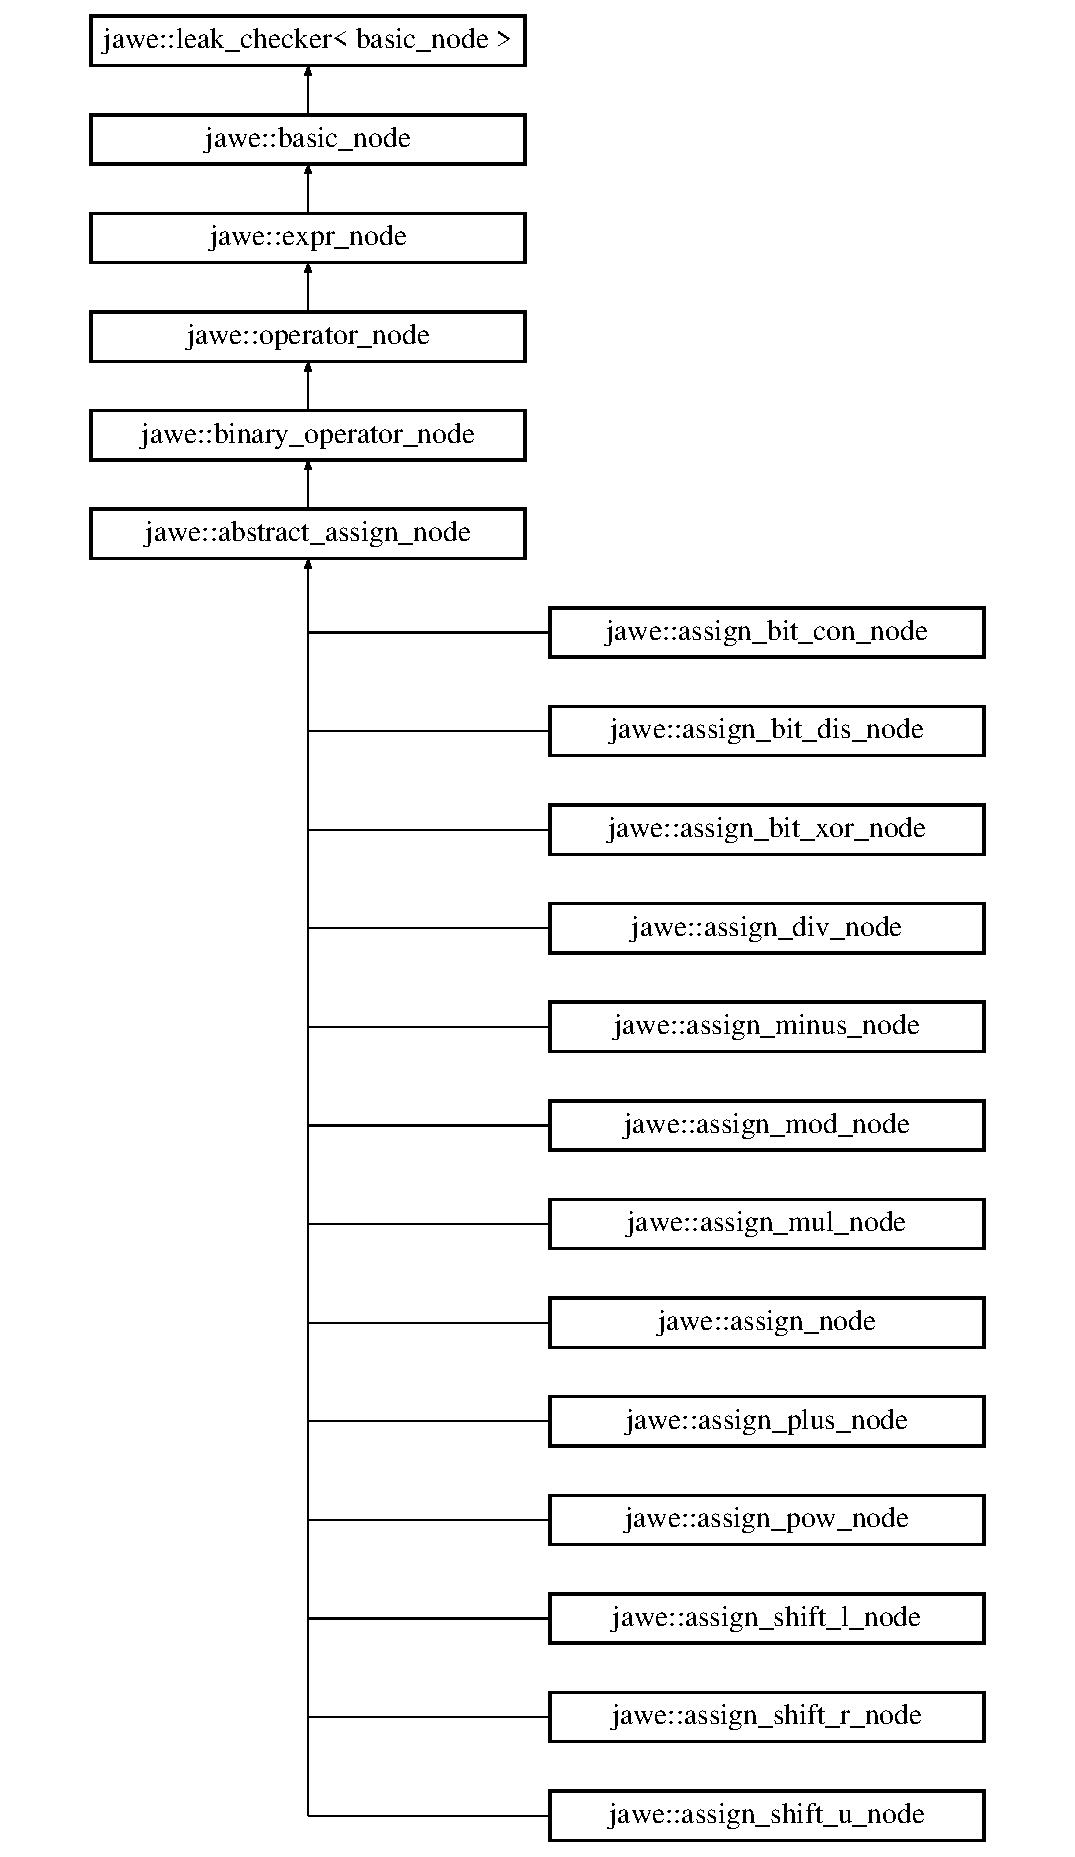
\includegraphics[height=12.000000cm]{classjawe_1_1abstract__assign__node}
\end{center}
\end{figure}
\subsection*{Public Member Functions}
\begin{DoxyCompactItemize}
\item 
\hyperlink{classjawe_1_1abstract__assign__node_ace18ba77e7a0d85b3b9c475062a8fec0}{abstract\+\_\+assign\+\_\+node} (const \hyperlink{namespacejawe_a3f307481d921b6cbb50cc8511fc2b544}{shared\+\_\+node} \&, const \hyperlink{namespacejawe_a3f307481d921b6cbb50cc8511fc2b544}{shared\+\_\+node} \&, std\+::string)
\end{DoxyCompactItemize}
\subsection*{Additional Inherited Members}


\subsection{Constructor \& Destructor Documentation}
\mbox{\Hypertarget{classjawe_1_1abstract__assign__node_ace18ba77e7a0d85b3b9c475062a8fec0}\label{classjawe_1_1abstract__assign__node_ace18ba77e7a0d85b3b9c475062a8fec0}} 
\index{jawe\+::abstract\+\_\+assign\+\_\+node@{jawe\+::abstract\+\_\+assign\+\_\+node}!abstract\+\_\+assign\+\_\+node@{abstract\+\_\+assign\+\_\+node}}
\index{abstract\+\_\+assign\+\_\+node@{abstract\+\_\+assign\+\_\+node}!jawe\+::abstract\+\_\+assign\+\_\+node@{jawe\+::abstract\+\_\+assign\+\_\+node}}
\subsubsection{\texorpdfstring{abstract\+\_\+assign\+\_\+node()}{abstract\_assign\_node()}}
{\footnotesize\ttfamily abstract\+\_\+assign\+\_\+node\+::abstract\+\_\+assign\+\_\+node (\begin{DoxyParamCaption}\item[{const \hyperlink{namespacejawe_a3f307481d921b6cbb50cc8511fc2b544}{shared\+\_\+node} \&}]{left,  }\item[{const \hyperlink{namespacejawe_a3f307481d921b6cbb50cc8511fc2b544}{shared\+\_\+node} \&}]{right,  }\item[{std\+::string}]{symbol }\end{DoxyParamCaption})}



The documentation for this class was generated from the following files\+:\begin{DoxyCompactItemize}
\item 
include/syntax/operators/\hyperlink{abstract__assign__node_8hpp}{abstract\+\_\+assign\+\_\+node.\+hpp}\item 
src/syntax/operators/\hyperlink{abstract__assign__node_8cpp}{abstract\+\_\+assign\+\_\+node.\+cpp}\end{DoxyCompactItemize}

\hypertarget{classjawe_1_1abstract__object__node}{}\section{jawe\+:\+:abstract\+\_\+object\+\_\+node Class Reference}
\label{classjawe_1_1abstract__object__node}\index{jawe\+::abstract\+\_\+object\+\_\+node@{jawe\+::abstract\+\_\+object\+\_\+node}}


{\ttfamily \#include $<$abstract\+\_\+object\+\_\+node.\+hpp$>$}

Inheritance diagram for jawe\+:\+:abstract\+\_\+object\+\_\+node\+:\begin{figure}[H]
\begin{center}
\leavevmode
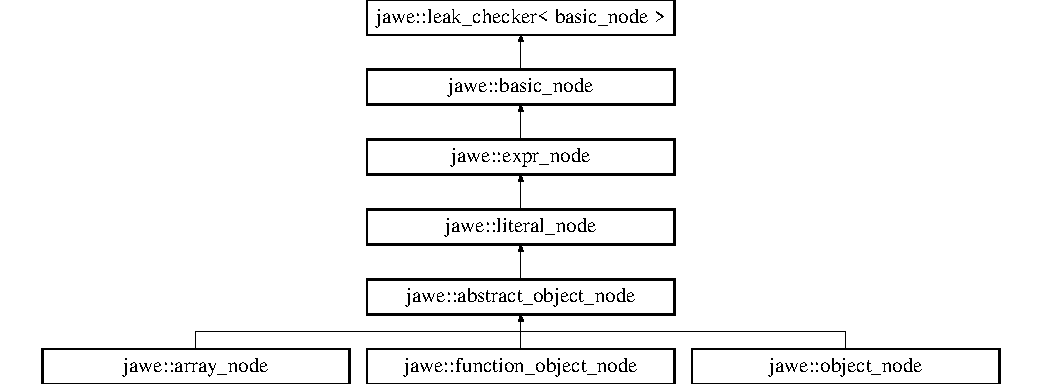
\includegraphics[height=5.161290cm]{classjawe_1_1abstract__object__node}
\end{center}
\end{figure}
\subsection*{Public Member Functions}
\begin{DoxyCompactItemize}
\item 
\hyperlink{classjawe_1_1abstract__object__node_a8450ead69438d87fbb72207407323da3}{abstract\+\_\+object\+\_\+node} (std\+::string)
\end{DoxyCompactItemize}
\subsection*{Additional Inherited Members}


\subsection{Constructor \& Destructor Documentation}
\mbox{\Hypertarget{classjawe_1_1abstract__object__node_a8450ead69438d87fbb72207407323da3}\label{classjawe_1_1abstract__object__node_a8450ead69438d87fbb72207407323da3}} 
\index{jawe\+::abstract\+\_\+object\+\_\+node@{jawe\+::abstract\+\_\+object\+\_\+node}!abstract\+\_\+object\+\_\+node@{abstract\+\_\+object\+\_\+node}}
\index{abstract\+\_\+object\+\_\+node@{abstract\+\_\+object\+\_\+node}!jawe\+::abstract\+\_\+object\+\_\+node@{jawe\+::abstract\+\_\+object\+\_\+node}}
\subsubsection{\texorpdfstring{abstract\+\_\+object\+\_\+node()}{abstract\_object\_node()}}
{\footnotesize\ttfamily abstract\+\_\+object\+\_\+node\+::abstract\+\_\+object\+\_\+node (\begin{DoxyParamCaption}\item[{std\+::string}]{symbol }\end{DoxyParamCaption})}



The documentation for this class was generated from the following files\+:\begin{DoxyCompactItemize}
\item 
include/syntax/literals/\hyperlink{abstract__object__node_8hpp}{abstract\+\_\+object\+\_\+node.\+hpp}\item 
src/syntax/literals/\hyperlink{abstract__object__node_8cpp}{abstract\+\_\+object\+\_\+node.\+cpp}\end{DoxyCompactItemize}

\hypertarget{classjawe_1_1array__access__node}{}\section{jawe\+:\+:array\+\_\+access\+\_\+node Class Reference}
\label{classjawe_1_1array__access__node}\index{jawe\+::array\+\_\+access\+\_\+node@{jawe\+::array\+\_\+access\+\_\+node}}


{\ttfamily \#include $<$array\+\_\+access\+\_\+node.\+hpp$>$}

Inheritance diagram for jawe\+:\+:array\+\_\+access\+\_\+node\+:\begin{figure}[H]
\begin{center}
\leavevmode
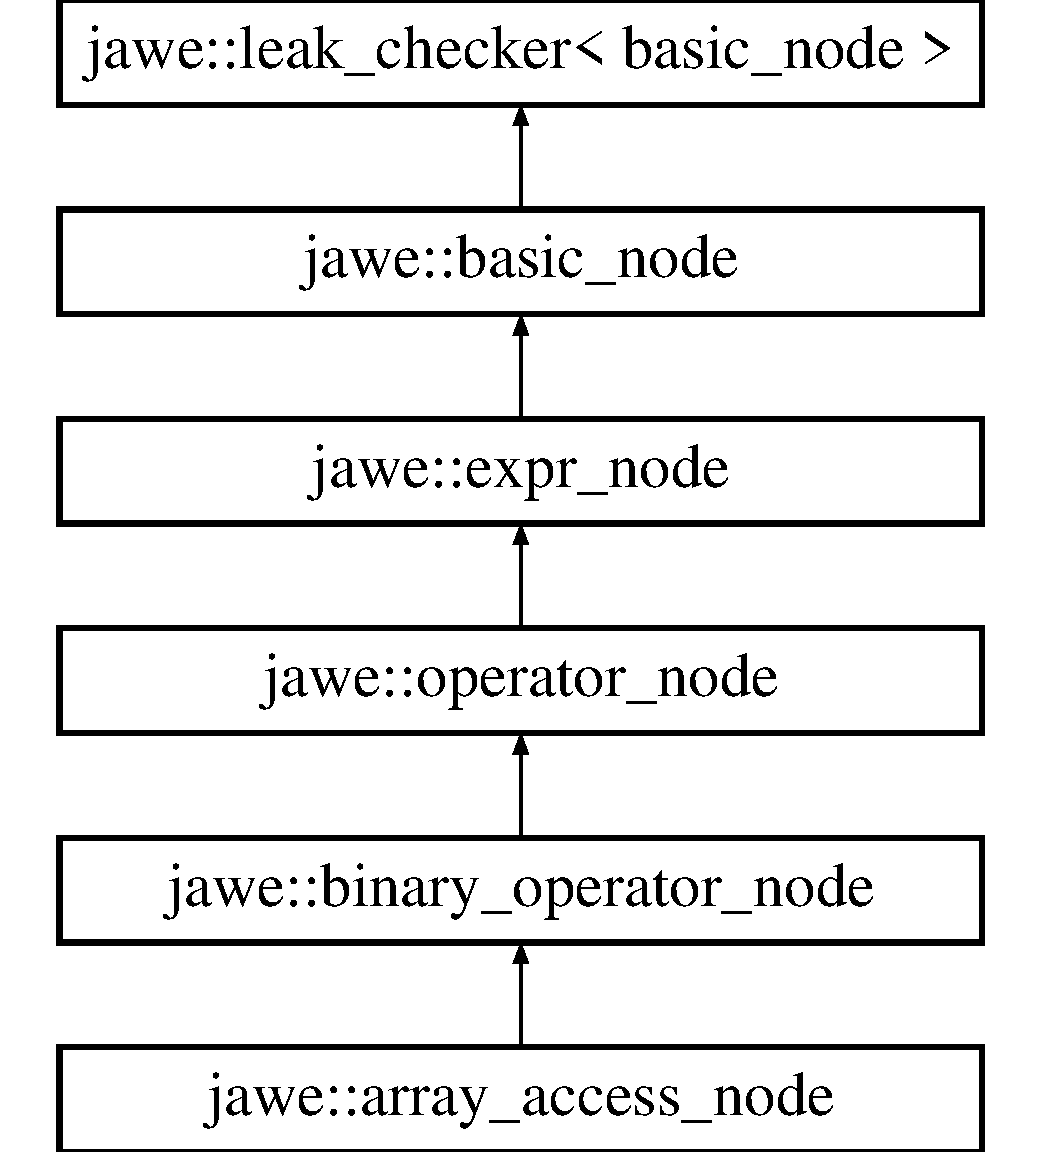
\includegraphics[height=6.000000cm]{classjawe_1_1array__access__node}
\end{center}
\end{figure}
\subsection*{Public Member Functions}
\begin{DoxyCompactItemize}
\item 
\hyperlink{classjawe_1_1array__access__node_a2befd67464439d2f94ee7469f41c5c1c}{array\+\_\+access\+\_\+node} (const \hyperlink{namespacejawe_a3f307481d921b6cbb50cc8511fc2b544}{shared\+\_\+node} \&, const \hyperlink{namespacejawe_a3f307481d921b6cbb50cc8511fc2b544}{shared\+\_\+node} \&)
\end{DoxyCompactItemize}
\subsection*{Additional Inherited Members}


\subsection{Constructor \& Destructor Documentation}
\mbox{\Hypertarget{classjawe_1_1array__access__node_a2befd67464439d2f94ee7469f41c5c1c}\label{classjawe_1_1array__access__node_a2befd67464439d2f94ee7469f41c5c1c}} 
\index{jawe\+::array\+\_\+access\+\_\+node@{jawe\+::array\+\_\+access\+\_\+node}!array\+\_\+access\+\_\+node@{array\+\_\+access\+\_\+node}}
\index{array\+\_\+access\+\_\+node@{array\+\_\+access\+\_\+node}!jawe\+::array\+\_\+access\+\_\+node@{jawe\+::array\+\_\+access\+\_\+node}}
\subsubsection{\texorpdfstring{array\+\_\+access\+\_\+node()}{array\_access\_node()}}
{\footnotesize\ttfamily array\+\_\+access\+\_\+node\+::array\+\_\+access\+\_\+node (\begin{DoxyParamCaption}\item[{const \hyperlink{namespacejawe_a3f307481d921b6cbb50cc8511fc2b544}{shared\+\_\+node} \&}]{left,  }\item[{const \hyperlink{namespacejawe_a3f307481d921b6cbb50cc8511fc2b544}{shared\+\_\+node} \&}]{right }\end{DoxyParamCaption})}



The documentation for this class was generated from the following files\+:\begin{DoxyCompactItemize}
\item 
include/syntax/operators/\hyperlink{array__access__node_8hpp}{array\+\_\+access\+\_\+node.\+hpp}\item 
src/syntax/operators/\hyperlink{array__access__node_8cpp}{array\+\_\+access\+\_\+node.\+cpp}\end{DoxyCompactItemize}

\hypertarget{classjawe_1_1array__node}{}\section{jawe\+:\+:array\+\_\+node Class Reference}
\label{classjawe_1_1array__node}\index{jawe\+::array\+\_\+node@{jawe\+::array\+\_\+node}}


{\ttfamily \#include $<$array\+\_\+node.\+hpp$>$}

Inheritance diagram for jawe\+:\+:array\+\_\+node\+:\begin{figure}[H]
\begin{center}
\leavevmode
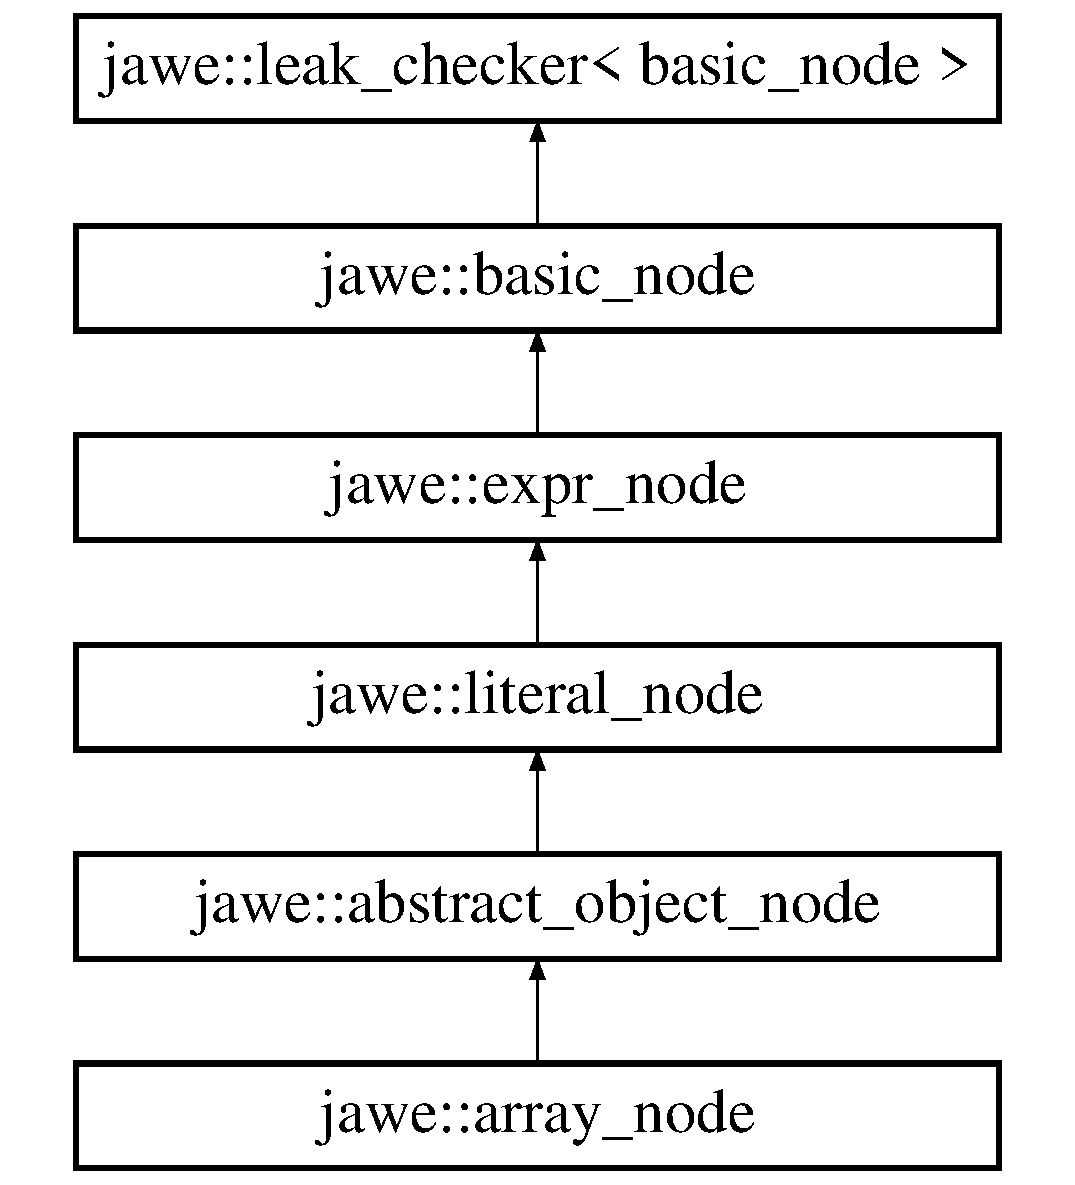
\includegraphics[height=6.000000cm]{classjawe_1_1array__node}
\end{center}
\end{figure}
\subsection*{Public Member Functions}
\begin{DoxyCompactItemize}
\item 
\hyperlink{classjawe_1_1array__node_ad9312ef54ed8588abf01fb6400201f04}{array\+\_\+node} ()
\item 
\hyperlink{classjawe_1_1array__node_af7f4791dfb0271ec0cce77c819069d84}{array\+\_\+node} (const std\+::vector$<$ \hyperlink{namespacejawe_a3f307481d921b6cbb50cc8511fc2b544}{shared\+\_\+node} $>$ \&)
\item 
void \hyperlink{classjawe_1_1array__node_af7c5ff9f67cb6601195cbc738c097239}{push\+\_\+back} (const \hyperlink{namespacejawe_a3f307481d921b6cbb50cc8511fc2b544}{shared\+\_\+node} \&)
\item 
std\+::vector$<$ \hyperlink{namespacejawe_a3f307481d921b6cbb50cc8511fc2b544}{shared\+\_\+node} $>$ \hyperlink{classjawe_1_1array__node_af83a0fd5093baee2db6e9aac615e9384}{get\+\_\+elements} ()
\end{DoxyCompactItemize}
\subsection*{Private Attributes}
\begin{DoxyCompactItemize}
\item 
std\+::vector$<$ \hyperlink{namespacejawe_a3f307481d921b6cbb50cc8511fc2b544}{shared\+\_\+node} $>$ \hyperlink{classjawe_1_1array__node_a13e0825e1f6f7334678c6f8a313532c2}{m\+\_\+elements}
\end{DoxyCompactItemize}
\subsection*{Additional Inherited Members}


\subsection{Constructor \& Destructor Documentation}
\mbox{\Hypertarget{classjawe_1_1array__node_ad9312ef54ed8588abf01fb6400201f04}\label{classjawe_1_1array__node_ad9312ef54ed8588abf01fb6400201f04}} 
\index{jawe\+::array\+\_\+node@{jawe\+::array\+\_\+node}!array\+\_\+node@{array\+\_\+node}}
\index{array\+\_\+node@{array\+\_\+node}!jawe\+::array\+\_\+node@{jawe\+::array\+\_\+node}}
\subsubsection{\texorpdfstring{array\+\_\+node()}{array\_node()}\hspace{0.1cm}{\footnotesize\ttfamily [1/2]}}
{\footnotesize\ttfamily array\+\_\+node\+::array\+\_\+node (\begin{DoxyParamCaption}{ }\end{DoxyParamCaption})}

\mbox{\Hypertarget{classjawe_1_1array__node_af7f4791dfb0271ec0cce77c819069d84}\label{classjawe_1_1array__node_af7f4791dfb0271ec0cce77c819069d84}} 
\index{jawe\+::array\+\_\+node@{jawe\+::array\+\_\+node}!array\+\_\+node@{array\+\_\+node}}
\index{array\+\_\+node@{array\+\_\+node}!jawe\+::array\+\_\+node@{jawe\+::array\+\_\+node}}
\subsubsection{\texorpdfstring{array\+\_\+node()}{array\_node()}\hspace{0.1cm}{\footnotesize\ttfamily [2/2]}}
{\footnotesize\ttfamily array\+\_\+node\+::array\+\_\+node (\begin{DoxyParamCaption}\item[{const std\+::vector$<$ \hyperlink{namespacejawe_a3f307481d921b6cbb50cc8511fc2b544}{shared\+\_\+node} $>$ \&}]{elements }\end{DoxyParamCaption})}



\subsection{Member Function Documentation}
\mbox{\Hypertarget{classjawe_1_1array__node_af83a0fd5093baee2db6e9aac615e9384}\label{classjawe_1_1array__node_af83a0fd5093baee2db6e9aac615e9384}} 
\index{jawe\+::array\+\_\+node@{jawe\+::array\+\_\+node}!get\+\_\+elements@{get\+\_\+elements}}
\index{get\+\_\+elements@{get\+\_\+elements}!jawe\+::array\+\_\+node@{jawe\+::array\+\_\+node}}
\subsubsection{\texorpdfstring{get\+\_\+elements()}{get\_elements()}}
{\footnotesize\ttfamily std\+::vector$<$ \hyperlink{namespacejawe_a3f307481d921b6cbb50cc8511fc2b544}{shared\+\_\+node} $>$ array\+\_\+node\+::get\+\_\+elements (\begin{DoxyParamCaption}{ }\end{DoxyParamCaption})}

\mbox{\Hypertarget{classjawe_1_1array__node_af7c5ff9f67cb6601195cbc738c097239}\label{classjawe_1_1array__node_af7c5ff9f67cb6601195cbc738c097239}} 
\index{jawe\+::array\+\_\+node@{jawe\+::array\+\_\+node}!push\+\_\+back@{push\+\_\+back}}
\index{push\+\_\+back@{push\+\_\+back}!jawe\+::array\+\_\+node@{jawe\+::array\+\_\+node}}
\subsubsection{\texorpdfstring{push\+\_\+back()}{push\_back()}}
{\footnotesize\ttfamily void array\+\_\+node\+::push\+\_\+back (\begin{DoxyParamCaption}\item[{const \hyperlink{namespacejawe_a3f307481d921b6cbb50cc8511fc2b544}{shared\+\_\+node} \&}]{expr }\end{DoxyParamCaption})}



\subsection{Member Data Documentation}
\mbox{\Hypertarget{classjawe_1_1array__node_a13e0825e1f6f7334678c6f8a313532c2}\label{classjawe_1_1array__node_a13e0825e1f6f7334678c6f8a313532c2}} 
\index{jawe\+::array\+\_\+node@{jawe\+::array\+\_\+node}!m\+\_\+elements@{m\+\_\+elements}}
\index{m\+\_\+elements@{m\+\_\+elements}!jawe\+::array\+\_\+node@{jawe\+::array\+\_\+node}}
\subsubsection{\texorpdfstring{m\+\_\+elements}{m\_elements}}
{\footnotesize\ttfamily std\+::vector$<$\hyperlink{namespacejawe_a3f307481d921b6cbb50cc8511fc2b544}{shared\+\_\+node}$>$ jawe\+::array\+\_\+node\+::m\+\_\+elements\hspace{0.3cm}{\ttfamily [private]}}



The documentation for this class was generated from the following files\+:\begin{DoxyCompactItemize}
\item 
include/syntax/literals/\hyperlink{array__node_8hpp}{array\+\_\+node.\+hpp}\item 
src/syntax/literals/\hyperlink{array__node_8cpp}{array\+\_\+node.\+cpp}\end{DoxyCompactItemize}

\hypertarget{classjawe_1_1assign__bit__con__node}{}\section{jawe\+:\+:assign\+\_\+bit\+\_\+con\+\_\+node Class Reference}
\label{classjawe_1_1assign__bit__con__node}\index{jawe\+::assign\+\_\+bit\+\_\+con\+\_\+node@{jawe\+::assign\+\_\+bit\+\_\+con\+\_\+node}}


{\ttfamily \#include $<$assign\+\_\+bit\+\_\+con\+\_\+node.\+hpp$>$}

Inheritance diagram for jawe\+:\+:assign\+\_\+bit\+\_\+con\+\_\+node\+:\begin{figure}[H]
\begin{center}
\leavevmode
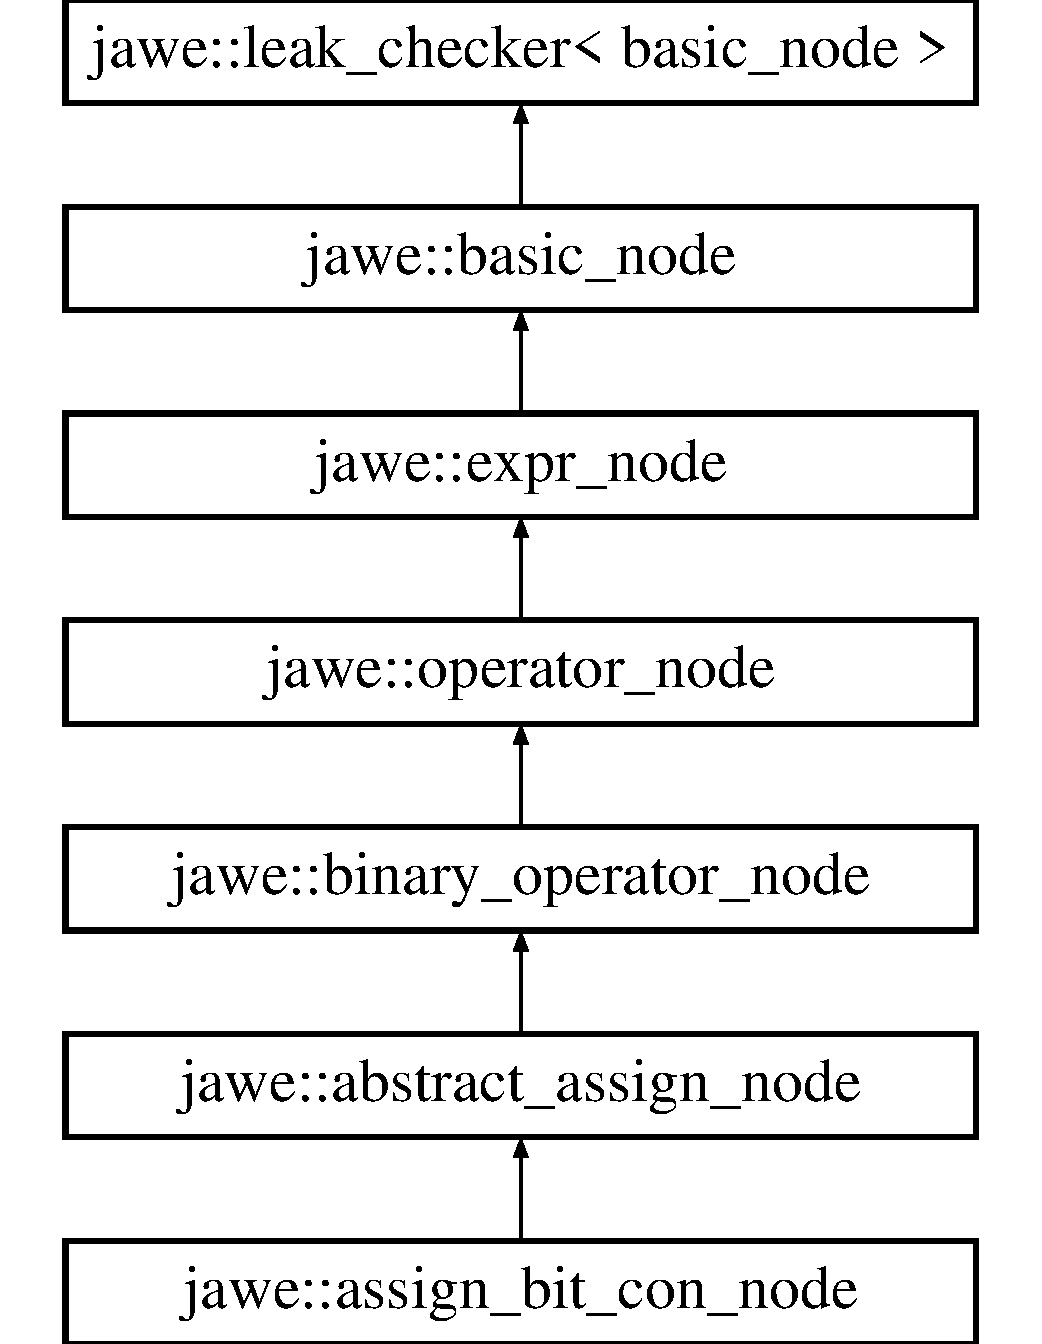
\includegraphics[height=7.000000cm]{classjawe_1_1assign__bit__con__node}
\end{center}
\end{figure}
\subsection*{Public Member Functions}
\begin{DoxyCompactItemize}
\item 
\hyperlink{classjawe_1_1assign__bit__con__node_a2fb255b81a19da94587320ae64d06ded}{assign\+\_\+bit\+\_\+con\+\_\+node} (const \hyperlink{namespacejawe_a3f307481d921b6cbb50cc8511fc2b544}{shared\+\_\+node} \&, const \hyperlink{namespacejawe_a3f307481d921b6cbb50cc8511fc2b544}{shared\+\_\+node} \&)
\end{DoxyCompactItemize}
\subsection*{Additional Inherited Members}


\subsection{Constructor \& Destructor Documentation}
\mbox{\Hypertarget{classjawe_1_1assign__bit__con__node_a2fb255b81a19da94587320ae64d06ded}\label{classjawe_1_1assign__bit__con__node_a2fb255b81a19da94587320ae64d06ded}} 
\index{jawe\+::assign\+\_\+bit\+\_\+con\+\_\+node@{jawe\+::assign\+\_\+bit\+\_\+con\+\_\+node}!assign\+\_\+bit\+\_\+con\+\_\+node@{assign\+\_\+bit\+\_\+con\+\_\+node}}
\index{assign\+\_\+bit\+\_\+con\+\_\+node@{assign\+\_\+bit\+\_\+con\+\_\+node}!jawe\+::assign\+\_\+bit\+\_\+con\+\_\+node@{jawe\+::assign\+\_\+bit\+\_\+con\+\_\+node}}
\subsubsection{\texorpdfstring{assign\+\_\+bit\+\_\+con\+\_\+node()}{assign\_bit\_con\_node()}}
{\footnotesize\ttfamily assign\+\_\+bit\+\_\+con\+\_\+node\+::assign\+\_\+bit\+\_\+con\+\_\+node (\begin{DoxyParamCaption}\item[{const \hyperlink{namespacejawe_a3f307481d921b6cbb50cc8511fc2b544}{shared\+\_\+node} \&}]{left,  }\item[{const \hyperlink{namespacejawe_a3f307481d921b6cbb50cc8511fc2b544}{shared\+\_\+node} \&}]{right }\end{DoxyParamCaption})}



The documentation for this class was generated from the following files\+:\begin{DoxyCompactItemize}
\item 
include/syntax/operators/\hyperlink{assign__bit__con__node_8hpp}{assign\+\_\+bit\+\_\+con\+\_\+node.\+hpp}\item 
src/syntax/operators/\hyperlink{assign__bit__con__node_8cpp}{assign\+\_\+bit\+\_\+con\+\_\+node.\+cpp}\end{DoxyCompactItemize}

\hypertarget{classjawe_1_1assign__bit__dis__node}{}\section{jawe\+:\+:assign\+\_\+bit\+\_\+dis\+\_\+node Class Reference}
\label{classjawe_1_1assign__bit__dis__node}\index{jawe\+::assign\+\_\+bit\+\_\+dis\+\_\+node@{jawe\+::assign\+\_\+bit\+\_\+dis\+\_\+node}}


{\ttfamily \#include $<$assign\+\_\+bit\+\_\+dis\+\_\+node.\+hpp$>$}

Inheritance diagram for jawe\+:\+:assign\+\_\+bit\+\_\+dis\+\_\+node\+:\begin{figure}[H]
\begin{center}
\leavevmode
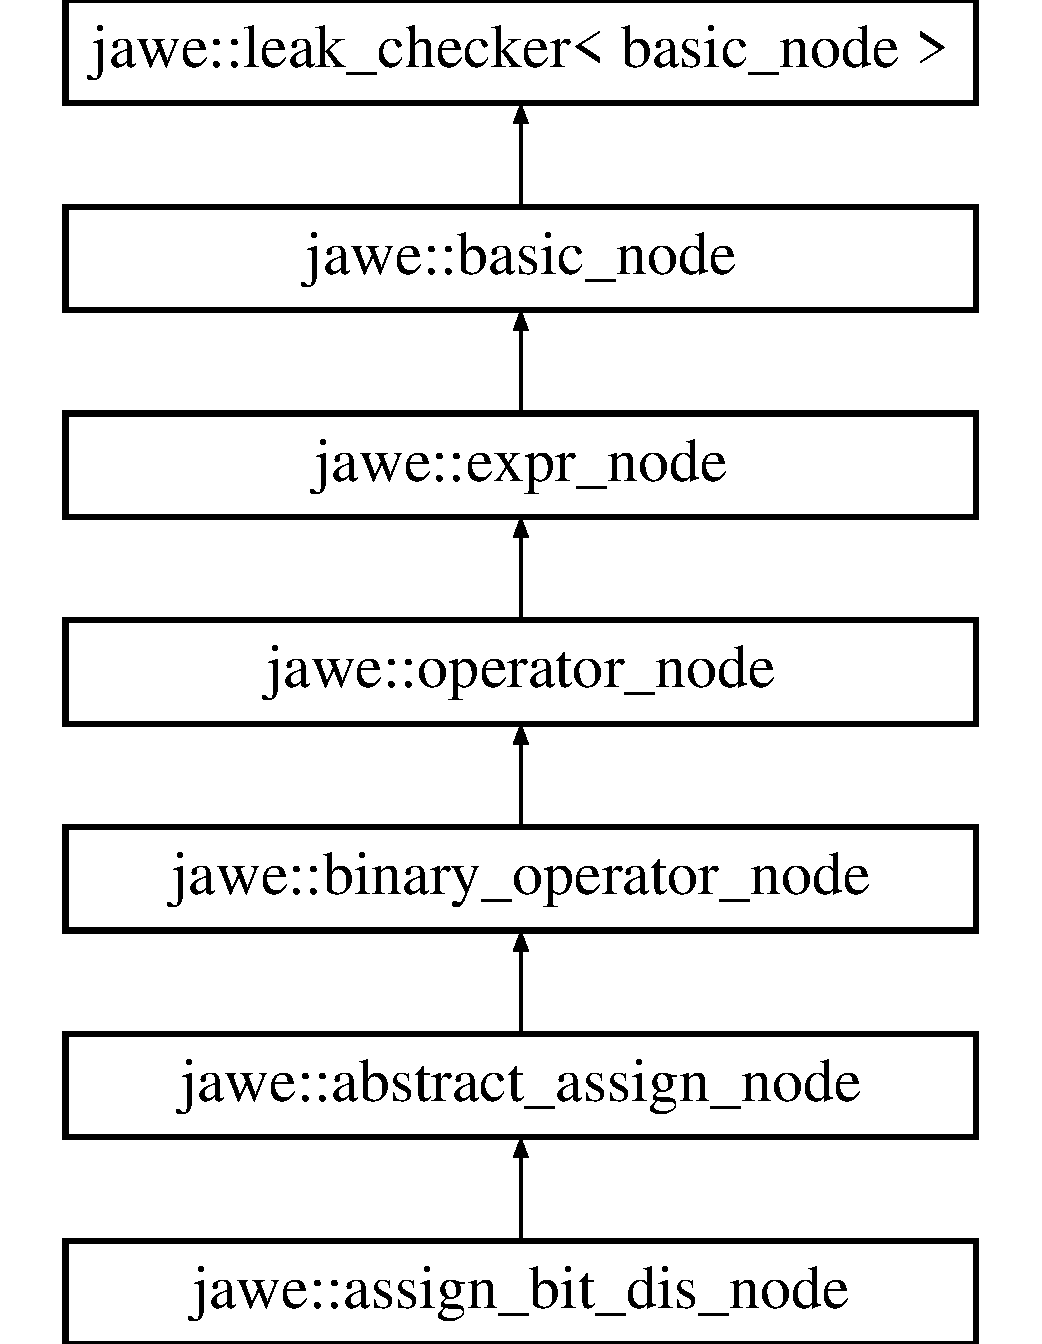
\includegraphics[height=7.000000cm]{classjawe_1_1assign__bit__dis__node}
\end{center}
\end{figure}
\subsection*{Public Member Functions}
\begin{DoxyCompactItemize}
\item 
\hyperlink{classjawe_1_1assign__bit__dis__node_afd0769ee76fe37456202382e3eb5537c}{assign\+\_\+bit\+\_\+dis\+\_\+node} (const \hyperlink{namespacejawe_a3f307481d921b6cbb50cc8511fc2b544}{shared\+\_\+node} \&, const \hyperlink{namespacejawe_a3f307481d921b6cbb50cc8511fc2b544}{shared\+\_\+node} \&)
\end{DoxyCompactItemize}
\subsection*{Additional Inherited Members}


\subsection{Constructor \& Destructor Documentation}
\mbox{\Hypertarget{classjawe_1_1assign__bit__dis__node_afd0769ee76fe37456202382e3eb5537c}\label{classjawe_1_1assign__bit__dis__node_afd0769ee76fe37456202382e3eb5537c}} 
\index{jawe\+::assign\+\_\+bit\+\_\+dis\+\_\+node@{jawe\+::assign\+\_\+bit\+\_\+dis\+\_\+node}!assign\+\_\+bit\+\_\+dis\+\_\+node@{assign\+\_\+bit\+\_\+dis\+\_\+node}}
\index{assign\+\_\+bit\+\_\+dis\+\_\+node@{assign\+\_\+bit\+\_\+dis\+\_\+node}!jawe\+::assign\+\_\+bit\+\_\+dis\+\_\+node@{jawe\+::assign\+\_\+bit\+\_\+dis\+\_\+node}}
\subsubsection{\texorpdfstring{assign\+\_\+bit\+\_\+dis\+\_\+node()}{assign\_bit\_dis\_node()}}
{\footnotesize\ttfamily assign\+\_\+bit\+\_\+dis\+\_\+node\+::assign\+\_\+bit\+\_\+dis\+\_\+node (\begin{DoxyParamCaption}\item[{const \hyperlink{namespacejawe_a3f307481d921b6cbb50cc8511fc2b544}{shared\+\_\+node} \&}]{left,  }\item[{const \hyperlink{namespacejawe_a3f307481d921b6cbb50cc8511fc2b544}{shared\+\_\+node} \&}]{right }\end{DoxyParamCaption})}



The documentation for this class was generated from the following files\+:\begin{DoxyCompactItemize}
\item 
include/syntax/operators/\hyperlink{assign__bit__dis__node_8hpp}{assign\+\_\+bit\+\_\+dis\+\_\+node.\+hpp}\item 
src/syntax/operators/\hyperlink{assign__bit__dis__node_8cpp}{assign\+\_\+bit\+\_\+dis\+\_\+node.\+cpp}\end{DoxyCompactItemize}

\hypertarget{classjawe_1_1assign__bit__xor__node}{}\section{jawe\+:\+:assign\+\_\+bit\+\_\+xor\+\_\+node Class Reference}
\label{classjawe_1_1assign__bit__xor__node}\index{jawe\+::assign\+\_\+bit\+\_\+xor\+\_\+node@{jawe\+::assign\+\_\+bit\+\_\+xor\+\_\+node}}


{\ttfamily \#include $<$assign\+\_\+bit\+\_\+xor\+\_\+node.\+hpp$>$}

Inheritance diagram for jawe\+:\+:assign\+\_\+bit\+\_\+xor\+\_\+node\+:\begin{figure}[H]
\begin{center}
\leavevmode
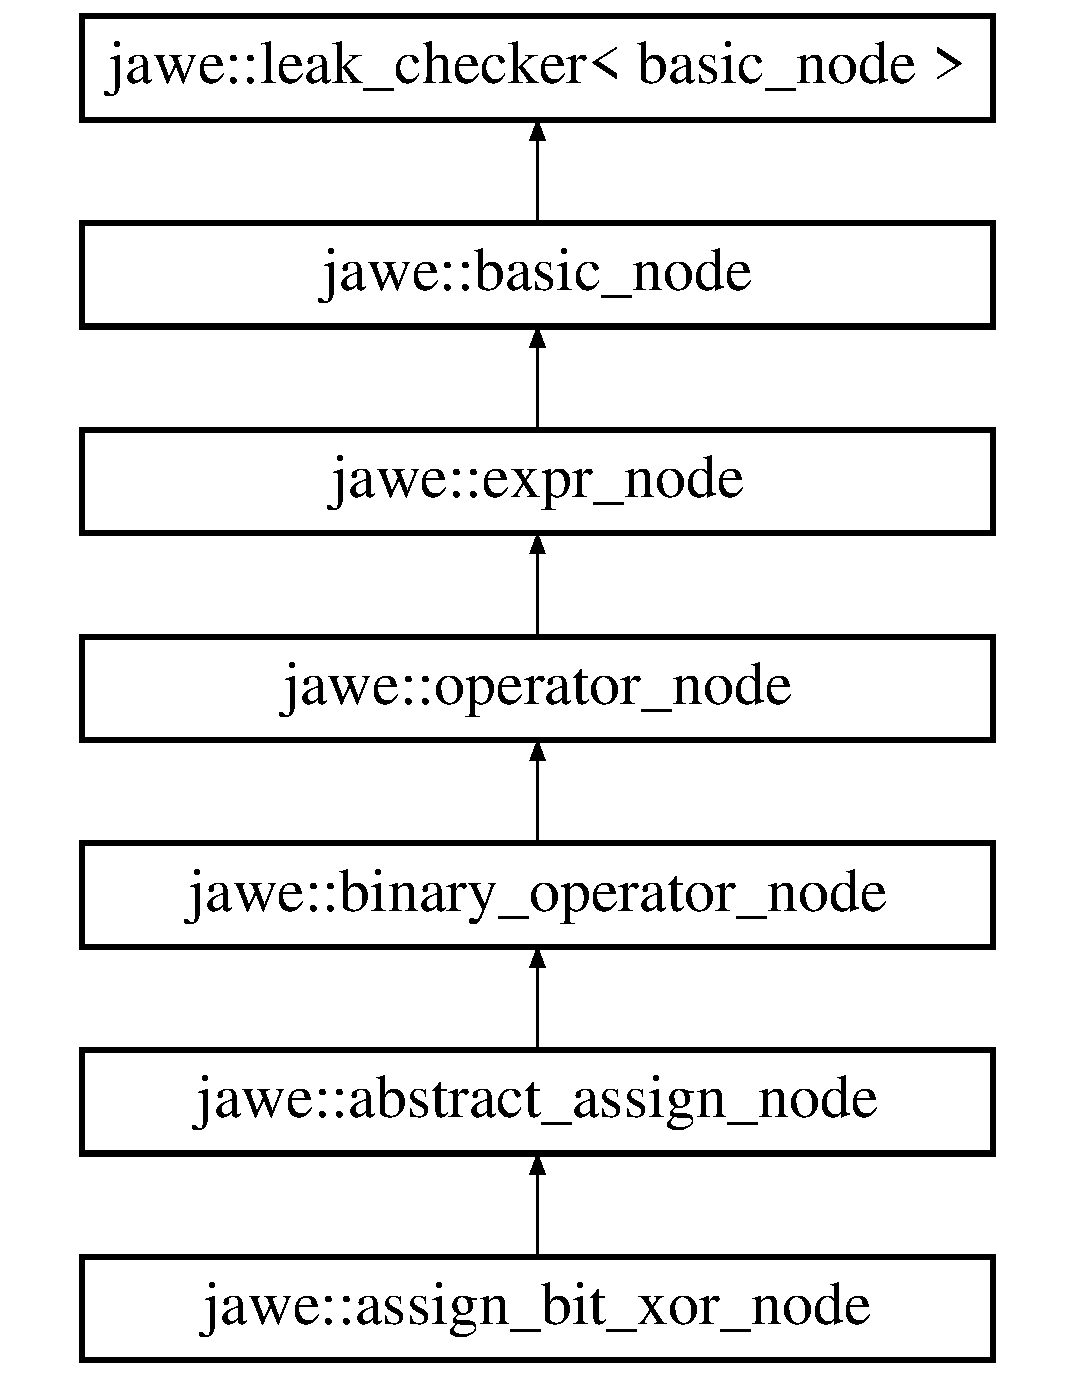
\includegraphics[height=7.000000cm]{classjawe_1_1assign__bit__xor__node}
\end{center}
\end{figure}
\subsection*{Public Member Functions}
\begin{DoxyCompactItemize}
\item 
\hyperlink{classjawe_1_1assign__bit__xor__node_ab8852a627f26d297efc252f4c31d2007}{assign\+\_\+bit\+\_\+xor\+\_\+node} (const \hyperlink{namespacejawe_a3f307481d921b6cbb50cc8511fc2b544}{shared\+\_\+node} \&, const \hyperlink{namespacejawe_a3f307481d921b6cbb50cc8511fc2b544}{shared\+\_\+node} \&)
\end{DoxyCompactItemize}
\subsection*{Additional Inherited Members}


\subsection{Constructor \& Destructor Documentation}
\mbox{\Hypertarget{classjawe_1_1assign__bit__xor__node_ab8852a627f26d297efc252f4c31d2007}\label{classjawe_1_1assign__bit__xor__node_ab8852a627f26d297efc252f4c31d2007}} 
\index{jawe\+::assign\+\_\+bit\+\_\+xor\+\_\+node@{jawe\+::assign\+\_\+bit\+\_\+xor\+\_\+node}!assign\+\_\+bit\+\_\+xor\+\_\+node@{assign\+\_\+bit\+\_\+xor\+\_\+node}}
\index{assign\+\_\+bit\+\_\+xor\+\_\+node@{assign\+\_\+bit\+\_\+xor\+\_\+node}!jawe\+::assign\+\_\+bit\+\_\+xor\+\_\+node@{jawe\+::assign\+\_\+bit\+\_\+xor\+\_\+node}}
\subsubsection{\texorpdfstring{assign\+\_\+bit\+\_\+xor\+\_\+node()}{assign\_bit\_xor\_node()}}
{\footnotesize\ttfamily assign\+\_\+bit\+\_\+xor\+\_\+node\+::assign\+\_\+bit\+\_\+xor\+\_\+node (\begin{DoxyParamCaption}\item[{const \hyperlink{namespacejawe_a3f307481d921b6cbb50cc8511fc2b544}{shared\+\_\+node} \&}]{left,  }\item[{const \hyperlink{namespacejawe_a3f307481d921b6cbb50cc8511fc2b544}{shared\+\_\+node} \&}]{right }\end{DoxyParamCaption})}



The documentation for this class was generated from the following files\+:\begin{DoxyCompactItemize}
\item 
include/syntax/operators/\hyperlink{assign__bit__xor__node_8hpp}{assign\+\_\+bit\+\_\+xor\+\_\+node.\+hpp}\item 
src/syntax/operators/\hyperlink{assign__bit__xor__node_8cpp}{assign\+\_\+bit\+\_\+xor\+\_\+node.\+cpp}\end{DoxyCompactItemize}

\hypertarget{classjawe_1_1assign__div__node}{}\section{jawe\+:\+:assign\+\_\+div\+\_\+node Class Reference}
\label{classjawe_1_1assign__div__node}\index{jawe\+::assign\+\_\+div\+\_\+node@{jawe\+::assign\+\_\+div\+\_\+node}}


{\ttfamily \#include $<$assign\+\_\+div\+\_\+node.\+hpp$>$}

Inheritance diagram for jawe\+:\+:assign\+\_\+div\+\_\+node\+:\begin{figure}[H]
\begin{center}
\leavevmode
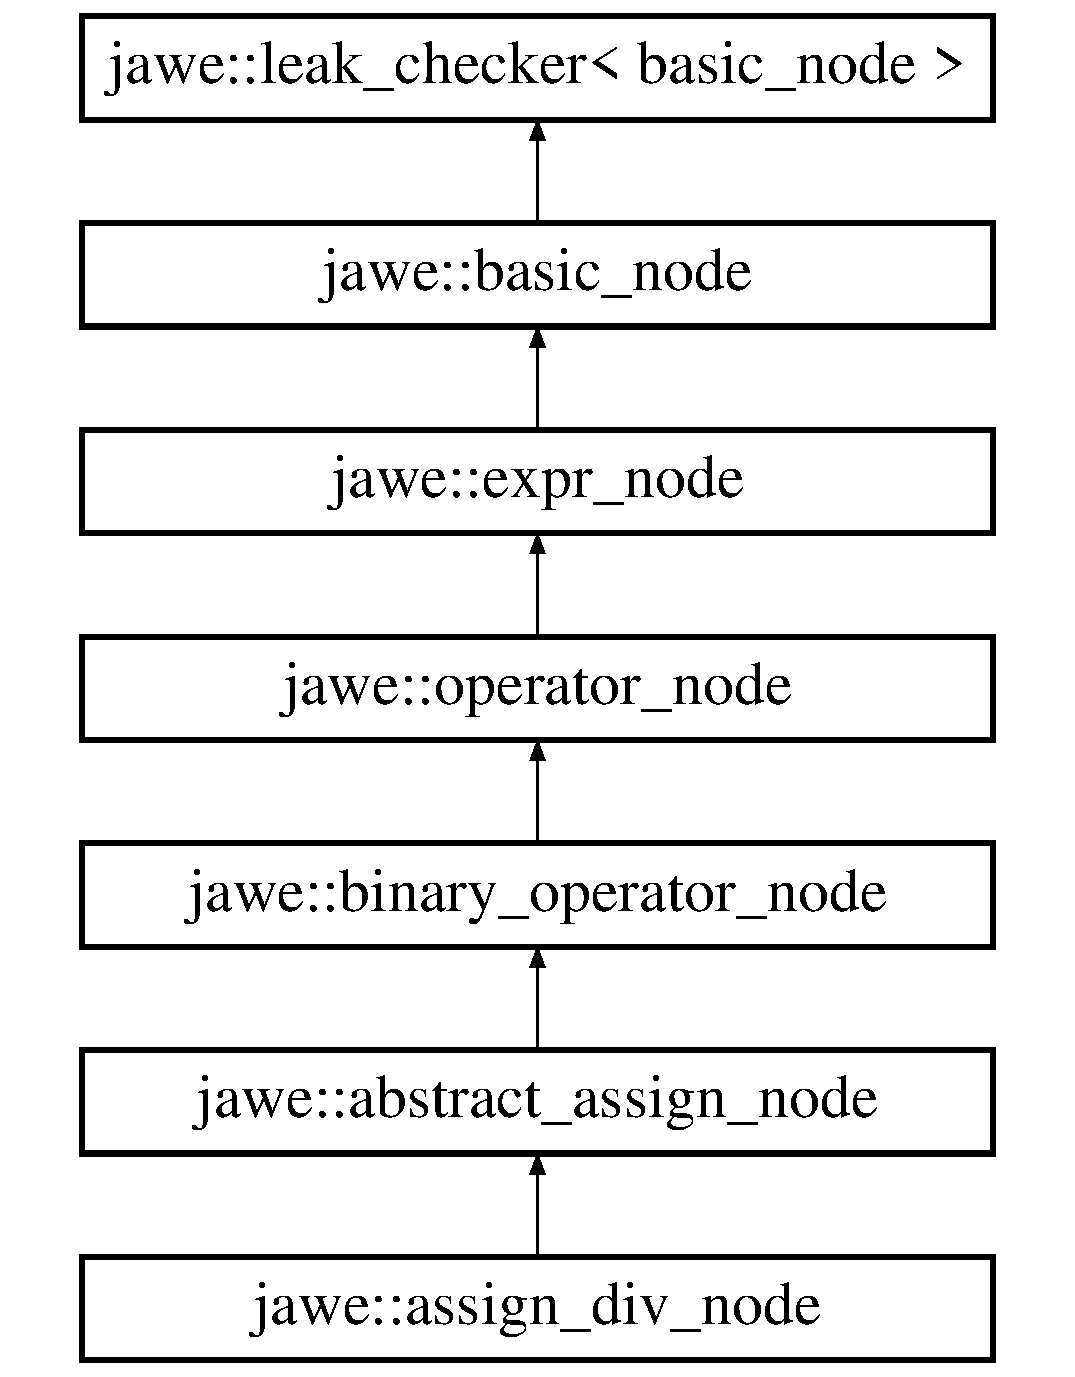
\includegraphics[height=7.000000cm]{classjawe_1_1assign__div__node}
\end{center}
\end{figure}
\subsection*{Public Member Functions}
\begin{DoxyCompactItemize}
\item 
\hyperlink{classjawe_1_1assign__div__node_a6c93a864f22c14973cd85fb0b682cee5}{assign\+\_\+div\+\_\+node} (const \hyperlink{namespacejawe_a3f307481d921b6cbb50cc8511fc2b544}{shared\+\_\+node} \&, const \hyperlink{namespacejawe_a3f307481d921b6cbb50cc8511fc2b544}{shared\+\_\+node} \&)
\end{DoxyCompactItemize}
\subsection*{Additional Inherited Members}


\subsection{Constructor \& Destructor Documentation}
\mbox{\Hypertarget{classjawe_1_1assign__div__node_a6c93a864f22c14973cd85fb0b682cee5}\label{classjawe_1_1assign__div__node_a6c93a864f22c14973cd85fb0b682cee5}} 
\index{jawe\+::assign\+\_\+div\+\_\+node@{jawe\+::assign\+\_\+div\+\_\+node}!assign\+\_\+div\+\_\+node@{assign\+\_\+div\+\_\+node}}
\index{assign\+\_\+div\+\_\+node@{assign\+\_\+div\+\_\+node}!jawe\+::assign\+\_\+div\+\_\+node@{jawe\+::assign\+\_\+div\+\_\+node}}
\subsubsection{\texorpdfstring{assign\+\_\+div\+\_\+node()}{assign\_div\_node()}}
{\footnotesize\ttfamily assign\+\_\+div\+\_\+node\+::assign\+\_\+div\+\_\+node (\begin{DoxyParamCaption}\item[{const \hyperlink{namespacejawe_a3f307481d921b6cbb50cc8511fc2b544}{shared\+\_\+node} \&}]{left,  }\item[{const \hyperlink{namespacejawe_a3f307481d921b6cbb50cc8511fc2b544}{shared\+\_\+node} \&}]{right }\end{DoxyParamCaption})}



The documentation for this class was generated from the following files\+:\begin{DoxyCompactItemize}
\item 
include/syntax/operators/\hyperlink{assign__div__node_8hpp}{assign\+\_\+div\+\_\+node.\+hpp}\item 
src/syntax/operators/\hyperlink{assign__div__node_8cpp}{assign\+\_\+div\+\_\+node.\+cpp}\end{DoxyCompactItemize}

\hypertarget{classjawe_1_1assign__minus__node}{}\section{jawe\+:\+:assign\+\_\+minus\+\_\+node Class Reference}
\label{classjawe_1_1assign__minus__node}\index{jawe\+::assign\+\_\+minus\+\_\+node@{jawe\+::assign\+\_\+minus\+\_\+node}}


{\ttfamily \#include $<$assign\+\_\+minus\+\_\+node.\+hpp$>$}

Inheritance diagram for jawe\+:\+:assign\+\_\+minus\+\_\+node\+:\begin{figure}[H]
\begin{center}
\leavevmode
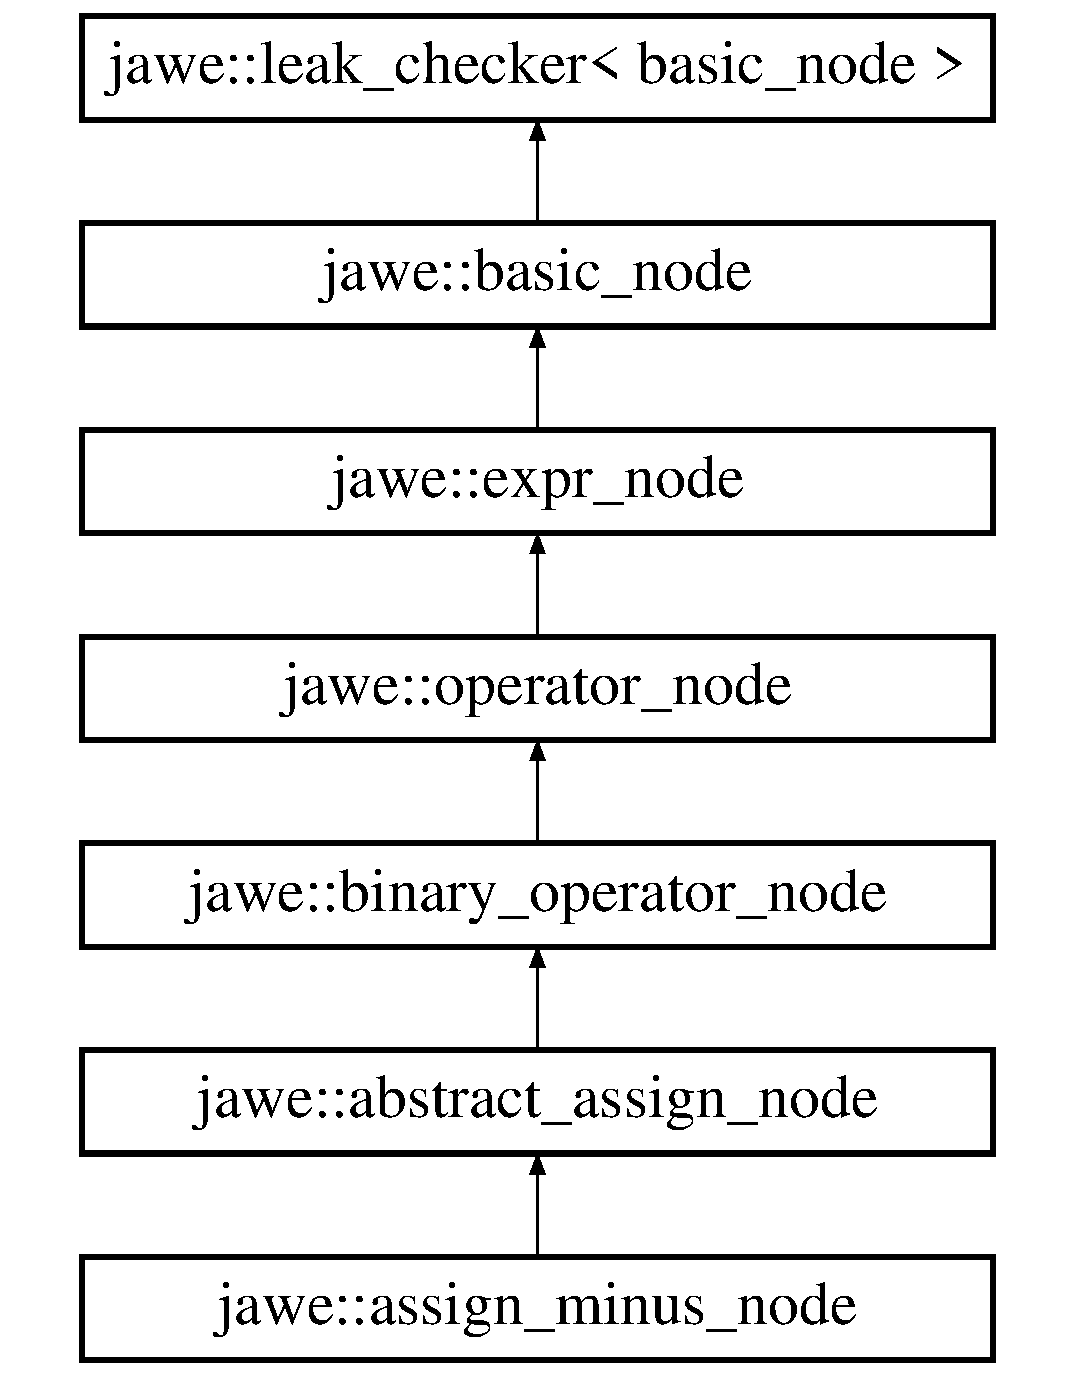
\includegraphics[height=7.000000cm]{classjawe_1_1assign__minus__node}
\end{center}
\end{figure}
\subsection*{Public Member Functions}
\begin{DoxyCompactItemize}
\item 
\hyperlink{classjawe_1_1assign__minus__node_a2af30fa677466e813e6816d26bad5706}{assign\+\_\+minus\+\_\+node} (const \hyperlink{namespacejawe_a3f307481d921b6cbb50cc8511fc2b544}{shared\+\_\+node} \&, const \hyperlink{namespacejawe_a3f307481d921b6cbb50cc8511fc2b544}{shared\+\_\+node} \&)
\end{DoxyCompactItemize}
\subsection*{Additional Inherited Members}


\subsection{Constructor \& Destructor Documentation}
\mbox{\Hypertarget{classjawe_1_1assign__minus__node_a2af30fa677466e813e6816d26bad5706}\label{classjawe_1_1assign__minus__node_a2af30fa677466e813e6816d26bad5706}} 
\index{jawe\+::assign\+\_\+minus\+\_\+node@{jawe\+::assign\+\_\+minus\+\_\+node}!assign\+\_\+minus\+\_\+node@{assign\+\_\+minus\+\_\+node}}
\index{assign\+\_\+minus\+\_\+node@{assign\+\_\+minus\+\_\+node}!jawe\+::assign\+\_\+minus\+\_\+node@{jawe\+::assign\+\_\+minus\+\_\+node}}
\subsubsection{\texorpdfstring{assign\+\_\+minus\+\_\+node()}{assign\_minus\_node()}}
{\footnotesize\ttfamily assign\+\_\+minus\+\_\+node\+::assign\+\_\+minus\+\_\+node (\begin{DoxyParamCaption}\item[{const \hyperlink{namespacejawe_a3f307481d921b6cbb50cc8511fc2b544}{shared\+\_\+node} \&}]{left,  }\item[{const \hyperlink{namespacejawe_a3f307481d921b6cbb50cc8511fc2b544}{shared\+\_\+node} \&}]{right }\end{DoxyParamCaption})}



The documentation for this class was generated from the following files\+:\begin{DoxyCompactItemize}
\item 
include/syntax/operators/\hyperlink{assign__minus__node_8hpp}{assign\+\_\+minus\+\_\+node.\+hpp}\item 
src/syntax/operators/\hyperlink{assign__minus__node_8cpp}{assign\+\_\+minus\+\_\+node.\+cpp}\end{DoxyCompactItemize}

\hypertarget{classjawe_1_1assign__mod__node}{}\section{jawe\+:\+:assign\+\_\+mod\+\_\+node Class Reference}
\label{classjawe_1_1assign__mod__node}\index{jawe\+::assign\+\_\+mod\+\_\+node@{jawe\+::assign\+\_\+mod\+\_\+node}}


{\ttfamily \#include $<$assign\+\_\+mod\+\_\+node.\+hpp$>$}

Inheritance diagram for jawe\+:\+:assign\+\_\+mod\+\_\+node\+:\begin{figure}[H]
\begin{center}
\leavevmode
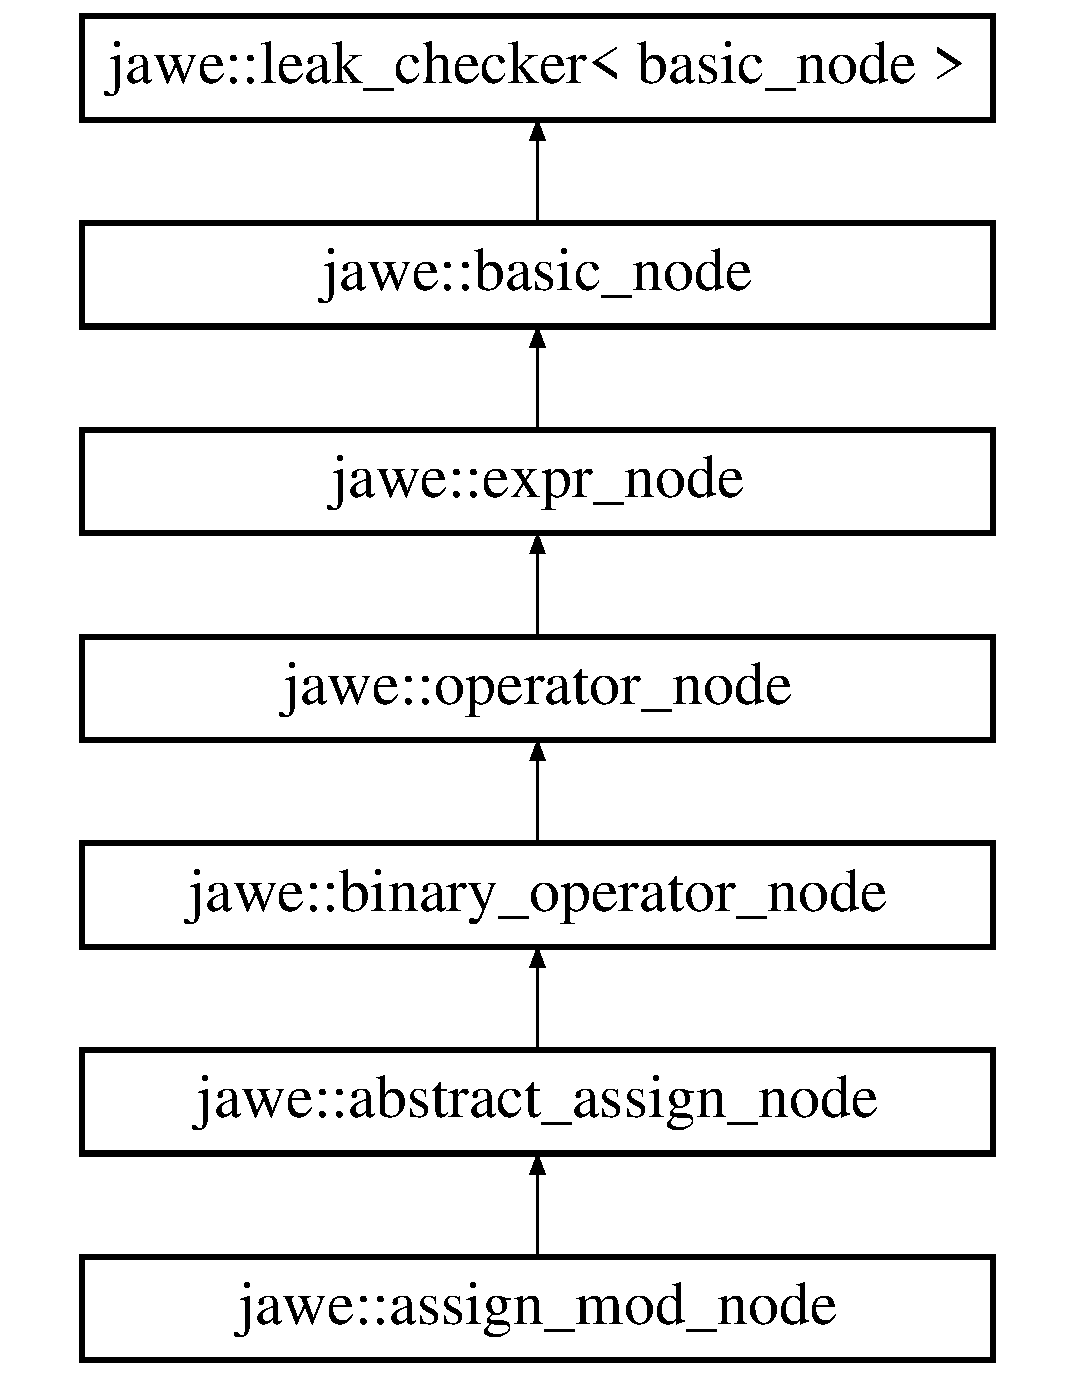
\includegraphics[height=7.000000cm]{classjawe_1_1assign__mod__node}
\end{center}
\end{figure}
\subsection*{Public Member Functions}
\begin{DoxyCompactItemize}
\item 
\hyperlink{classjawe_1_1assign__mod__node_a61568b3132d7dbff69208f0be51f7bf4}{assign\+\_\+mod\+\_\+node} (const \hyperlink{namespacejawe_a3f307481d921b6cbb50cc8511fc2b544}{shared\+\_\+node} \&, const \hyperlink{namespacejawe_a3f307481d921b6cbb50cc8511fc2b544}{shared\+\_\+node} \&)
\end{DoxyCompactItemize}
\subsection*{Additional Inherited Members}


\subsection{Constructor \& Destructor Documentation}
\mbox{\Hypertarget{classjawe_1_1assign__mod__node_a61568b3132d7dbff69208f0be51f7bf4}\label{classjawe_1_1assign__mod__node_a61568b3132d7dbff69208f0be51f7bf4}} 
\index{jawe\+::assign\+\_\+mod\+\_\+node@{jawe\+::assign\+\_\+mod\+\_\+node}!assign\+\_\+mod\+\_\+node@{assign\+\_\+mod\+\_\+node}}
\index{assign\+\_\+mod\+\_\+node@{assign\+\_\+mod\+\_\+node}!jawe\+::assign\+\_\+mod\+\_\+node@{jawe\+::assign\+\_\+mod\+\_\+node}}
\subsubsection{\texorpdfstring{assign\+\_\+mod\+\_\+node()}{assign\_mod\_node()}}
{\footnotesize\ttfamily assign\+\_\+mod\+\_\+node\+::assign\+\_\+mod\+\_\+node (\begin{DoxyParamCaption}\item[{const \hyperlink{namespacejawe_a3f307481d921b6cbb50cc8511fc2b544}{shared\+\_\+node} \&}]{left,  }\item[{const \hyperlink{namespacejawe_a3f307481d921b6cbb50cc8511fc2b544}{shared\+\_\+node} \&}]{right }\end{DoxyParamCaption})}



The documentation for this class was generated from the following files\+:\begin{DoxyCompactItemize}
\item 
include/syntax/operators/\hyperlink{assign__mod__node_8hpp}{assign\+\_\+mod\+\_\+node.\+hpp}\item 
src/syntax/operators/\hyperlink{assign__mod__node_8cpp}{assign\+\_\+mod\+\_\+node.\+cpp}\end{DoxyCompactItemize}

\hypertarget{classjawe_1_1assign__mul__node}{}\section{jawe\+:\+:assign\+\_\+mul\+\_\+node Class Reference}
\label{classjawe_1_1assign__mul__node}\index{jawe\+::assign\+\_\+mul\+\_\+node@{jawe\+::assign\+\_\+mul\+\_\+node}}


{\ttfamily \#include $<$assign\+\_\+mul\+\_\+node.\+hpp$>$}

Inheritance diagram for jawe\+:\+:assign\+\_\+mul\+\_\+node\+:\begin{figure}[H]
\begin{center}
\leavevmode
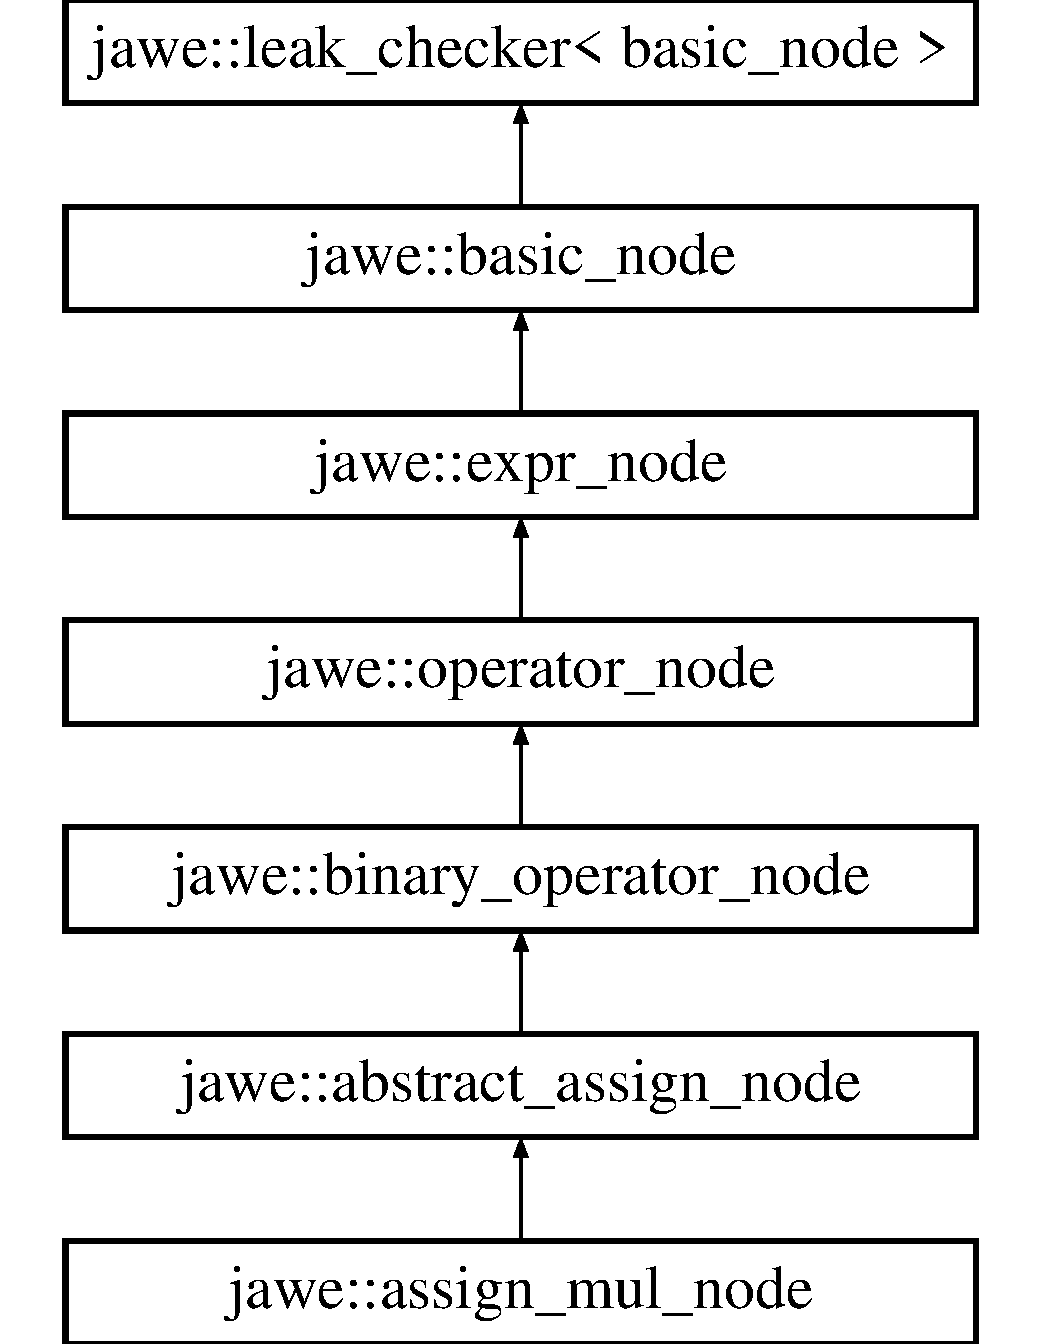
\includegraphics[height=7.000000cm]{classjawe_1_1assign__mul__node}
\end{center}
\end{figure}
\subsection*{Public Member Functions}
\begin{DoxyCompactItemize}
\item 
\hyperlink{classjawe_1_1assign__mul__node_a865cd6732dc4eb59ba3f280b5b171997}{assign\+\_\+mul\+\_\+node} (const \hyperlink{namespacejawe_a3f307481d921b6cbb50cc8511fc2b544}{shared\+\_\+node} \&, const \hyperlink{namespacejawe_a3f307481d921b6cbb50cc8511fc2b544}{shared\+\_\+node} \&)
\end{DoxyCompactItemize}
\subsection*{Additional Inherited Members}


\subsection{Constructor \& Destructor Documentation}
\mbox{\Hypertarget{classjawe_1_1assign__mul__node_a865cd6732dc4eb59ba3f280b5b171997}\label{classjawe_1_1assign__mul__node_a865cd6732dc4eb59ba3f280b5b171997}} 
\index{jawe\+::assign\+\_\+mul\+\_\+node@{jawe\+::assign\+\_\+mul\+\_\+node}!assign\+\_\+mul\+\_\+node@{assign\+\_\+mul\+\_\+node}}
\index{assign\+\_\+mul\+\_\+node@{assign\+\_\+mul\+\_\+node}!jawe\+::assign\+\_\+mul\+\_\+node@{jawe\+::assign\+\_\+mul\+\_\+node}}
\subsubsection{\texorpdfstring{assign\+\_\+mul\+\_\+node()}{assign\_mul\_node()}}
{\footnotesize\ttfamily assign\+\_\+mul\+\_\+node\+::assign\+\_\+mul\+\_\+node (\begin{DoxyParamCaption}\item[{const \hyperlink{namespacejawe_a3f307481d921b6cbb50cc8511fc2b544}{shared\+\_\+node} \&}]{left,  }\item[{const \hyperlink{namespacejawe_a3f307481d921b6cbb50cc8511fc2b544}{shared\+\_\+node} \&}]{right }\end{DoxyParamCaption})}



The documentation for this class was generated from the following files\+:\begin{DoxyCompactItemize}
\item 
include/syntax/operators/\hyperlink{assign__mul__node_8hpp}{assign\+\_\+mul\+\_\+node.\+hpp}\item 
src/syntax/operators/\hyperlink{assign__mul__node_8cpp}{assign\+\_\+mul\+\_\+node.\+cpp}\end{DoxyCompactItemize}

\hypertarget{classjawe_1_1assign__node}{}\section{jawe\+:\+:assign\+\_\+node Class Reference}
\label{classjawe_1_1assign__node}\index{jawe\+::assign\+\_\+node@{jawe\+::assign\+\_\+node}}


{\ttfamily \#include $<$assign\+\_\+node.\+hpp$>$}

Inheritance diagram for jawe\+:\+:assign\+\_\+node\+:\begin{figure}[H]
\begin{center}
\leavevmode
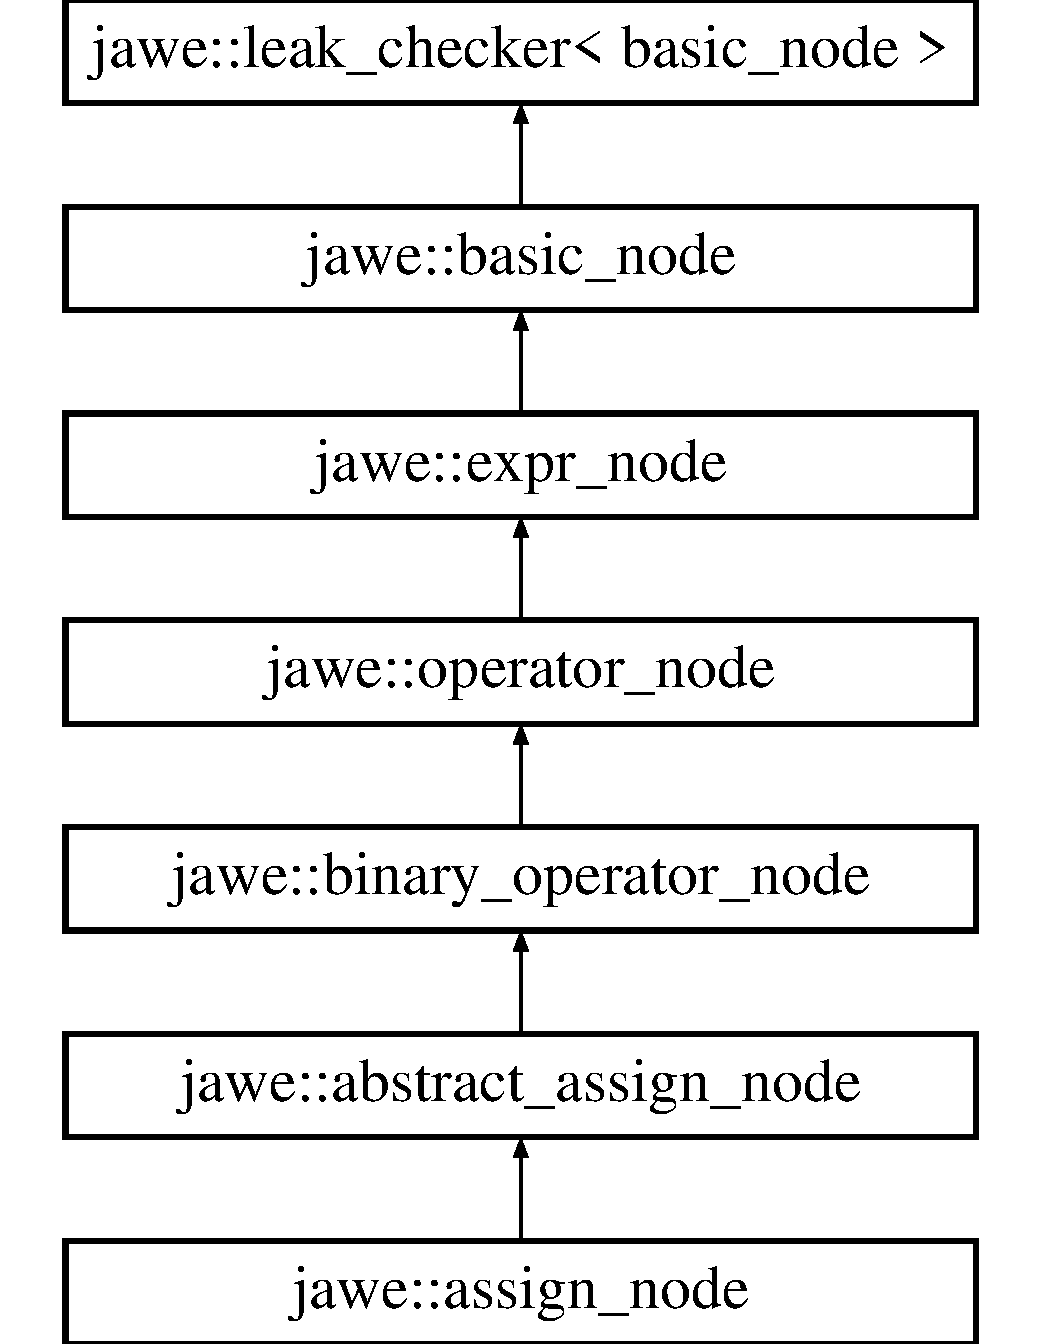
\includegraphics[height=7.000000cm]{classjawe_1_1assign__node}
\end{center}
\end{figure}
\subsection*{Public Member Functions}
\begin{DoxyCompactItemize}
\item 
\hyperlink{classjawe_1_1assign__node_a68c98f0414966b2fafca90bb6a7e8725}{assign\+\_\+node} (const \hyperlink{namespacejawe_a3f307481d921b6cbb50cc8511fc2b544}{shared\+\_\+node} \&, const \hyperlink{namespacejawe_a3f307481d921b6cbb50cc8511fc2b544}{shared\+\_\+node} \&)
\end{DoxyCompactItemize}
\subsection*{Additional Inherited Members}


\subsection{Constructor \& Destructor Documentation}
\mbox{\Hypertarget{classjawe_1_1assign__node_a68c98f0414966b2fafca90bb6a7e8725}\label{classjawe_1_1assign__node_a68c98f0414966b2fafca90bb6a7e8725}} 
\index{jawe\+::assign\+\_\+node@{jawe\+::assign\+\_\+node}!assign\+\_\+node@{assign\+\_\+node}}
\index{assign\+\_\+node@{assign\+\_\+node}!jawe\+::assign\+\_\+node@{jawe\+::assign\+\_\+node}}
\subsubsection{\texorpdfstring{assign\+\_\+node()}{assign\_node()}}
{\footnotesize\ttfamily assign\+\_\+node\+::assign\+\_\+node (\begin{DoxyParamCaption}\item[{const \hyperlink{namespacejawe_a3f307481d921b6cbb50cc8511fc2b544}{shared\+\_\+node} \&}]{left,  }\item[{const \hyperlink{namespacejawe_a3f307481d921b6cbb50cc8511fc2b544}{shared\+\_\+node} \&}]{right }\end{DoxyParamCaption})}



The documentation for this class was generated from the following files\+:\begin{DoxyCompactItemize}
\item 
include/syntax/operators/\hyperlink{assign__node_8hpp}{assign\+\_\+node.\+hpp}\item 
src/syntax/operators/\hyperlink{assign__node_8cpp}{assign\+\_\+node.\+cpp}\end{DoxyCompactItemize}

\hypertarget{classjawe_1_1assign__plus__node}{}\section{jawe\+:\+:assign\+\_\+plus\+\_\+node Class Reference}
\label{classjawe_1_1assign__plus__node}\index{jawe\+::assign\+\_\+plus\+\_\+node@{jawe\+::assign\+\_\+plus\+\_\+node}}


{\ttfamily \#include $<$assign\+\_\+plus\+\_\+node.\+hpp$>$}

Inheritance diagram for jawe\+:\+:assign\+\_\+plus\+\_\+node\+:\begin{figure}[H]
\begin{center}
\leavevmode
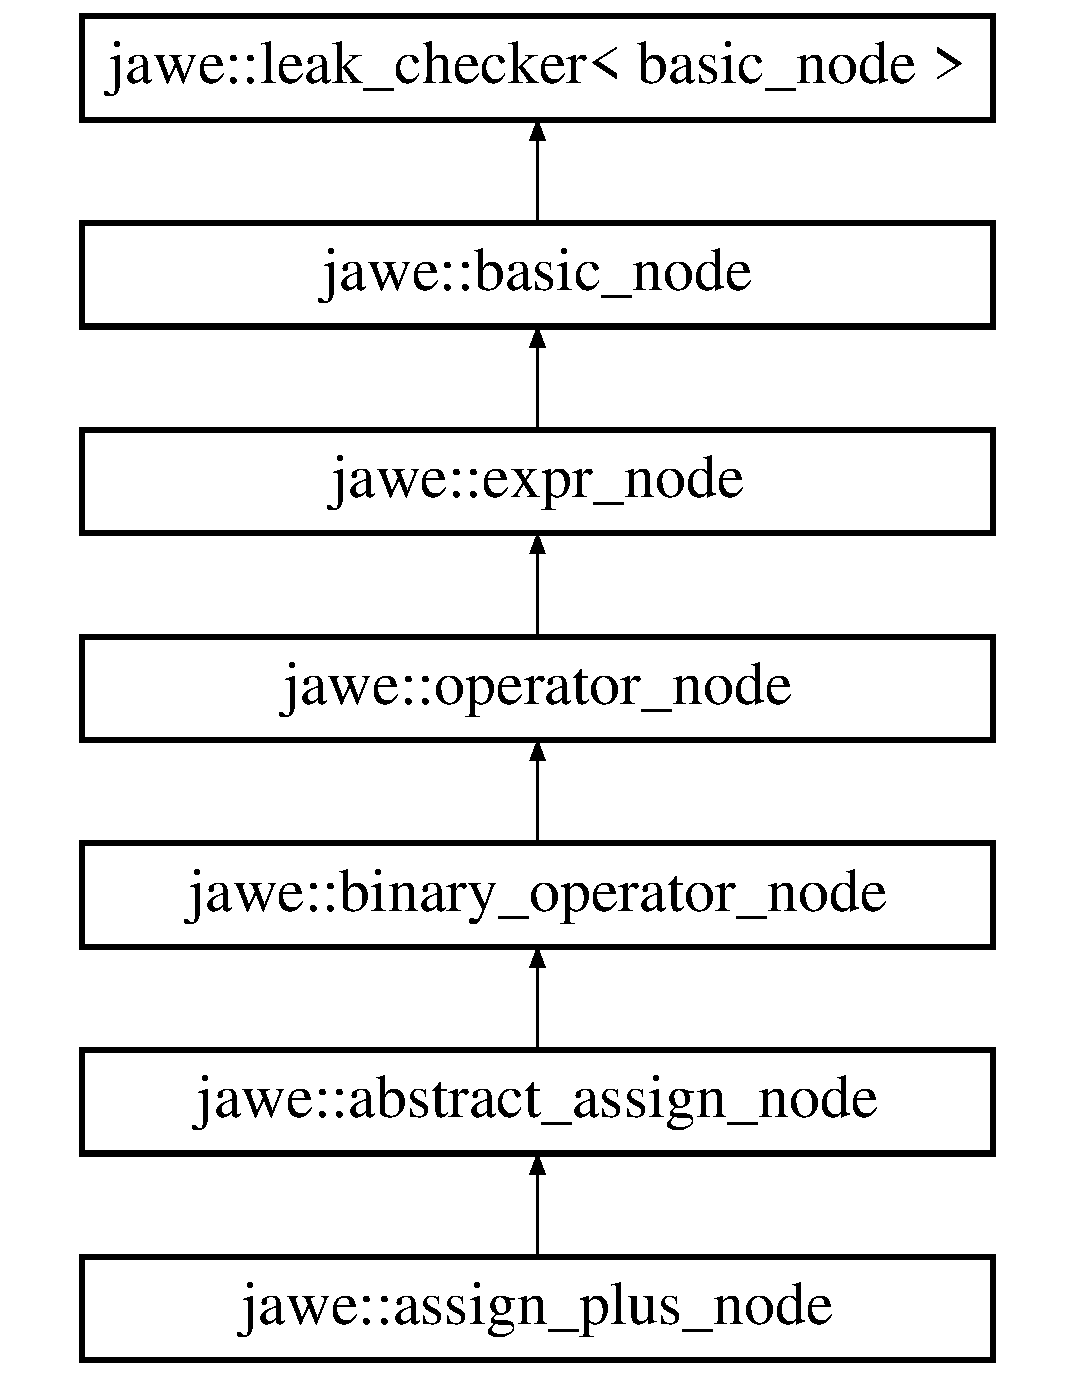
\includegraphics[height=7.000000cm]{classjawe_1_1assign__plus__node}
\end{center}
\end{figure}
\subsection*{Public Member Functions}
\begin{DoxyCompactItemize}
\item 
\hyperlink{classjawe_1_1assign__plus__node_a15d9635bfd0dd4cc3ca1a20829ff31f5}{assign\+\_\+plus\+\_\+node} (const \hyperlink{namespacejawe_a3f307481d921b6cbb50cc8511fc2b544}{shared\+\_\+node} \&, const \hyperlink{namespacejawe_a3f307481d921b6cbb50cc8511fc2b544}{shared\+\_\+node} \&)
\end{DoxyCompactItemize}
\subsection*{Additional Inherited Members}


\subsection{Constructor \& Destructor Documentation}
\mbox{\Hypertarget{classjawe_1_1assign__plus__node_a15d9635bfd0dd4cc3ca1a20829ff31f5}\label{classjawe_1_1assign__plus__node_a15d9635bfd0dd4cc3ca1a20829ff31f5}} 
\index{jawe\+::assign\+\_\+plus\+\_\+node@{jawe\+::assign\+\_\+plus\+\_\+node}!assign\+\_\+plus\+\_\+node@{assign\+\_\+plus\+\_\+node}}
\index{assign\+\_\+plus\+\_\+node@{assign\+\_\+plus\+\_\+node}!jawe\+::assign\+\_\+plus\+\_\+node@{jawe\+::assign\+\_\+plus\+\_\+node}}
\subsubsection{\texorpdfstring{assign\+\_\+plus\+\_\+node()}{assign\_plus\_node()}}
{\footnotesize\ttfamily assign\+\_\+plus\+\_\+node\+::assign\+\_\+plus\+\_\+node (\begin{DoxyParamCaption}\item[{const \hyperlink{namespacejawe_a3f307481d921b6cbb50cc8511fc2b544}{shared\+\_\+node} \&}]{left,  }\item[{const \hyperlink{namespacejawe_a3f307481d921b6cbb50cc8511fc2b544}{shared\+\_\+node} \&}]{right }\end{DoxyParamCaption})}



The documentation for this class was generated from the following files\+:\begin{DoxyCompactItemize}
\item 
include/syntax/operators/\hyperlink{assign__plus__node_8hpp}{assign\+\_\+plus\+\_\+node.\+hpp}\item 
src/syntax/operators/\hyperlink{assign__plus__node_8cpp}{assign\+\_\+plus\+\_\+node.\+cpp}\end{DoxyCompactItemize}

\hypertarget{classjawe_1_1assign__pow__node}{}\section{jawe\+:\+:assign\+\_\+pow\+\_\+node Class Reference}
\label{classjawe_1_1assign__pow__node}\index{jawe\+::assign\+\_\+pow\+\_\+node@{jawe\+::assign\+\_\+pow\+\_\+node}}


{\ttfamily \#include $<$assign\+\_\+pow\+\_\+node.\+hpp$>$}

Inheritance diagram for jawe\+:\+:assign\+\_\+pow\+\_\+node\+:\begin{figure}[H]
\begin{center}
\leavevmode
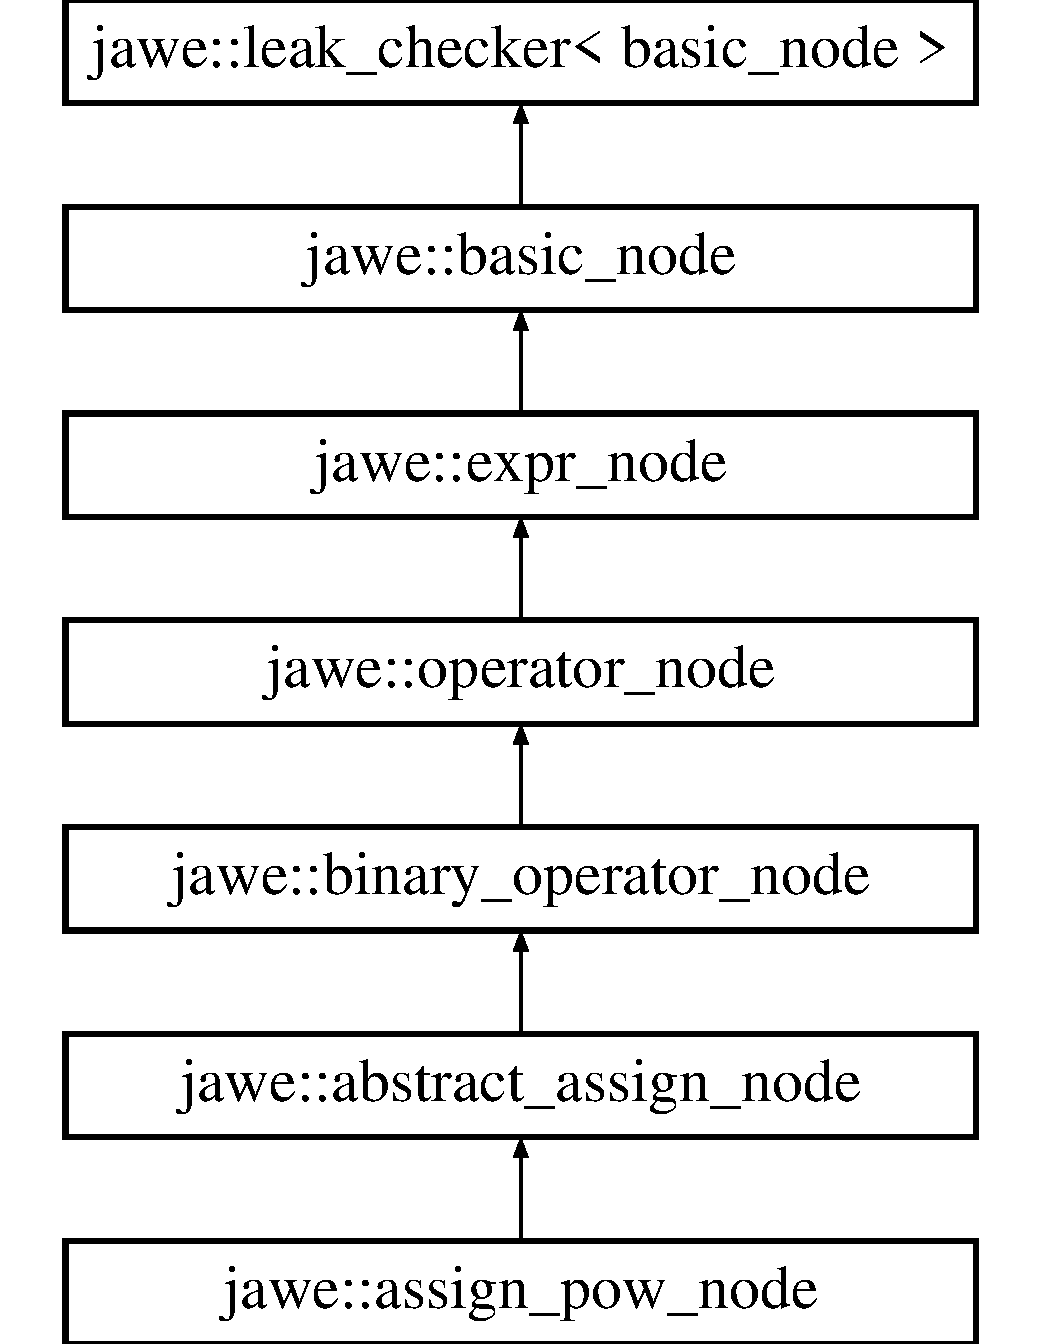
\includegraphics[height=7.000000cm]{classjawe_1_1assign__pow__node}
\end{center}
\end{figure}
\subsection*{Public Member Functions}
\begin{DoxyCompactItemize}
\item 
\hyperlink{classjawe_1_1assign__pow__node_acb02ec954455cce18c9280a54c0afbf7}{assign\+\_\+pow\+\_\+node} (const \hyperlink{namespacejawe_a3f307481d921b6cbb50cc8511fc2b544}{shared\+\_\+node} \&, const \hyperlink{namespacejawe_a3f307481d921b6cbb50cc8511fc2b544}{shared\+\_\+node} \&)
\end{DoxyCompactItemize}
\subsection*{Additional Inherited Members}


\subsection{Constructor \& Destructor Documentation}
\mbox{\Hypertarget{classjawe_1_1assign__pow__node_acb02ec954455cce18c9280a54c0afbf7}\label{classjawe_1_1assign__pow__node_acb02ec954455cce18c9280a54c0afbf7}} 
\index{jawe\+::assign\+\_\+pow\+\_\+node@{jawe\+::assign\+\_\+pow\+\_\+node}!assign\+\_\+pow\+\_\+node@{assign\+\_\+pow\+\_\+node}}
\index{assign\+\_\+pow\+\_\+node@{assign\+\_\+pow\+\_\+node}!jawe\+::assign\+\_\+pow\+\_\+node@{jawe\+::assign\+\_\+pow\+\_\+node}}
\subsubsection{\texorpdfstring{assign\+\_\+pow\+\_\+node()}{assign\_pow\_node()}}
{\footnotesize\ttfamily assign\+\_\+pow\+\_\+node\+::assign\+\_\+pow\+\_\+node (\begin{DoxyParamCaption}\item[{const \hyperlink{namespacejawe_a3f307481d921b6cbb50cc8511fc2b544}{shared\+\_\+node} \&}]{left,  }\item[{const \hyperlink{namespacejawe_a3f307481d921b6cbb50cc8511fc2b544}{shared\+\_\+node} \&}]{right }\end{DoxyParamCaption})}



The documentation for this class was generated from the following files\+:\begin{DoxyCompactItemize}
\item 
include/syntax/operators/\hyperlink{assign__pow__node_8hpp}{assign\+\_\+pow\+\_\+node.\+hpp}\item 
src/syntax/operators/\hyperlink{assign__pow__node_8cpp}{assign\+\_\+pow\+\_\+node.\+cpp}\end{DoxyCompactItemize}

\hypertarget{classjawe_1_1assign__shift__l__node}{}\section{jawe\+:\+:assign\+\_\+shift\+\_\+l\+\_\+node Class Reference}
\label{classjawe_1_1assign__shift__l__node}\index{jawe\+::assign\+\_\+shift\+\_\+l\+\_\+node@{jawe\+::assign\+\_\+shift\+\_\+l\+\_\+node}}


{\ttfamily \#include $<$assign\+\_\+shift\+\_\+l\+\_\+node.\+hpp$>$}

Inheritance diagram for jawe\+:\+:assign\+\_\+shift\+\_\+l\+\_\+node\+:\begin{figure}[H]
\begin{center}
\leavevmode
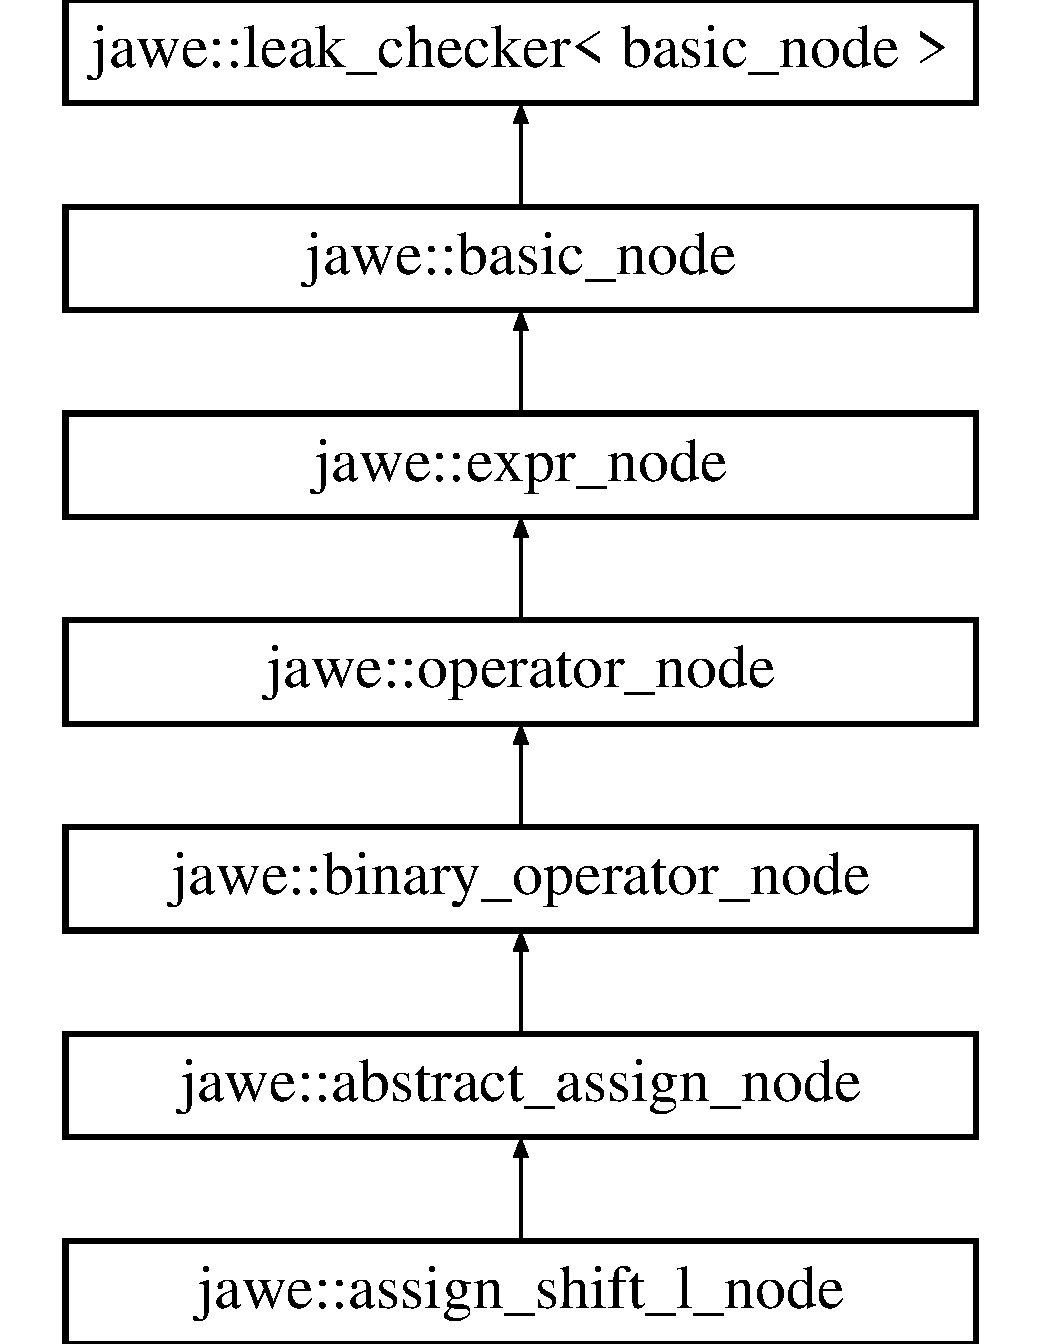
\includegraphics[height=7.000000cm]{classjawe_1_1assign__shift__l__node}
\end{center}
\end{figure}
\subsection*{Public Member Functions}
\begin{DoxyCompactItemize}
\item 
\hyperlink{classjawe_1_1assign__shift__l__node_a2080d7988468a35784e84850b5dcc60a}{assign\+\_\+shift\+\_\+l\+\_\+node} (const \hyperlink{namespacejawe_a3f307481d921b6cbb50cc8511fc2b544}{shared\+\_\+node} \&, const \hyperlink{namespacejawe_a3f307481d921b6cbb50cc8511fc2b544}{shared\+\_\+node} \&)
\end{DoxyCompactItemize}
\subsection*{Additional Inherited Members}


\subsection{Constructor \& Destructor Documentation}
\mbox{\Hypertarget{classjawe_1_1assign__shift__l__node_a2080d7988468a35784e84850b5dcc60a}\label{classjawe_1_1assign__shift__l__node_a2080d7988468a35784e84850b5dcc60a}} 
\index{jawe\+::assign\+\_\+shift\+\_\+l\+\_\+node@{jawe\+::assign\+\_\+shift\+\_\+l\+\_\+node}!assign\+\_\+shift\+\_\+l\+\_\+node@{assign\+\_\+shift\+\_\+l\+\_\+node}}
\index{assign\+\_\+shift\+\_\+l\+\_\+node@{assign\+\_\+shift\+\_\+l\+\_\+node}!jawe\+::assign\+\_\+shift\+\_\+l\+\_\+node@{jawe\+::assign\+\_\+shift\+\_\+l\+\_\+node}}
\subsubsection{\texorpdfstring{assign\+\_\+shift\+\_\+l\+\_\+node()}{assign\_shift\_l\_node()}}
{\footnotesize\ttfamily assign\+\_\+shift\+\_\+l\+\_\+node\+::assign\+\_\+shift\+\_\+l\+\_\+node (\begin{DoxyParamCaption}\item[{const \hyperlink{namespacejawe_a3f307481d921b6cbb50cc8511fc2b544}{shared\+\_\+node} \&}]{left,  }\item[{const \hyperlink{namespacejawe_a3f307481d921b6cbb50cc8511fc2b544}{shared\+\_\+node} \&}]{right }\end{DoxyParamCaption})}



The documentation for this class was generated from the following files\+:\begin{DoxyCompactItemize}
\item 
include/syntax/operators/\hyperlink{assign__shift__l__node_8hpp}{assign\+\_\+shift\+\_\+l\+\_\+node.\+hpp}\item 
src/syntax/operators/\hyperlink{assign__shift__l__node_8cpp}{assign\+\_\+shift\+\_\+l\+\_\+node.\+cpp}\end{DoxyCompactItemize}

\hypertarget{classjawe_1_1assign__shift__r__node}{}\section{jawe\+:\+:assign\+\_\+shift\+\_\+r\+\_\+node Class Reference}
\label{classjawe_1_1assign__shift__r__node}\index{jawe\+::assign\+\_\+shift\+\_\+r\+\_\+node@{jawe\+::assign\+\_\+shift\+\_\+r\+\_\+node}}


{\ttfamily \#include $<$assign\+\_\+shift\+\_\+r\+\_\+node.\+hpp$>$}

Inheritance diagram for jawe\+:\+:assign\+\_\+shift\+\_\+r\+\_\+node\+:\begin{figure}[H]
\begin{center}
\leavevmode
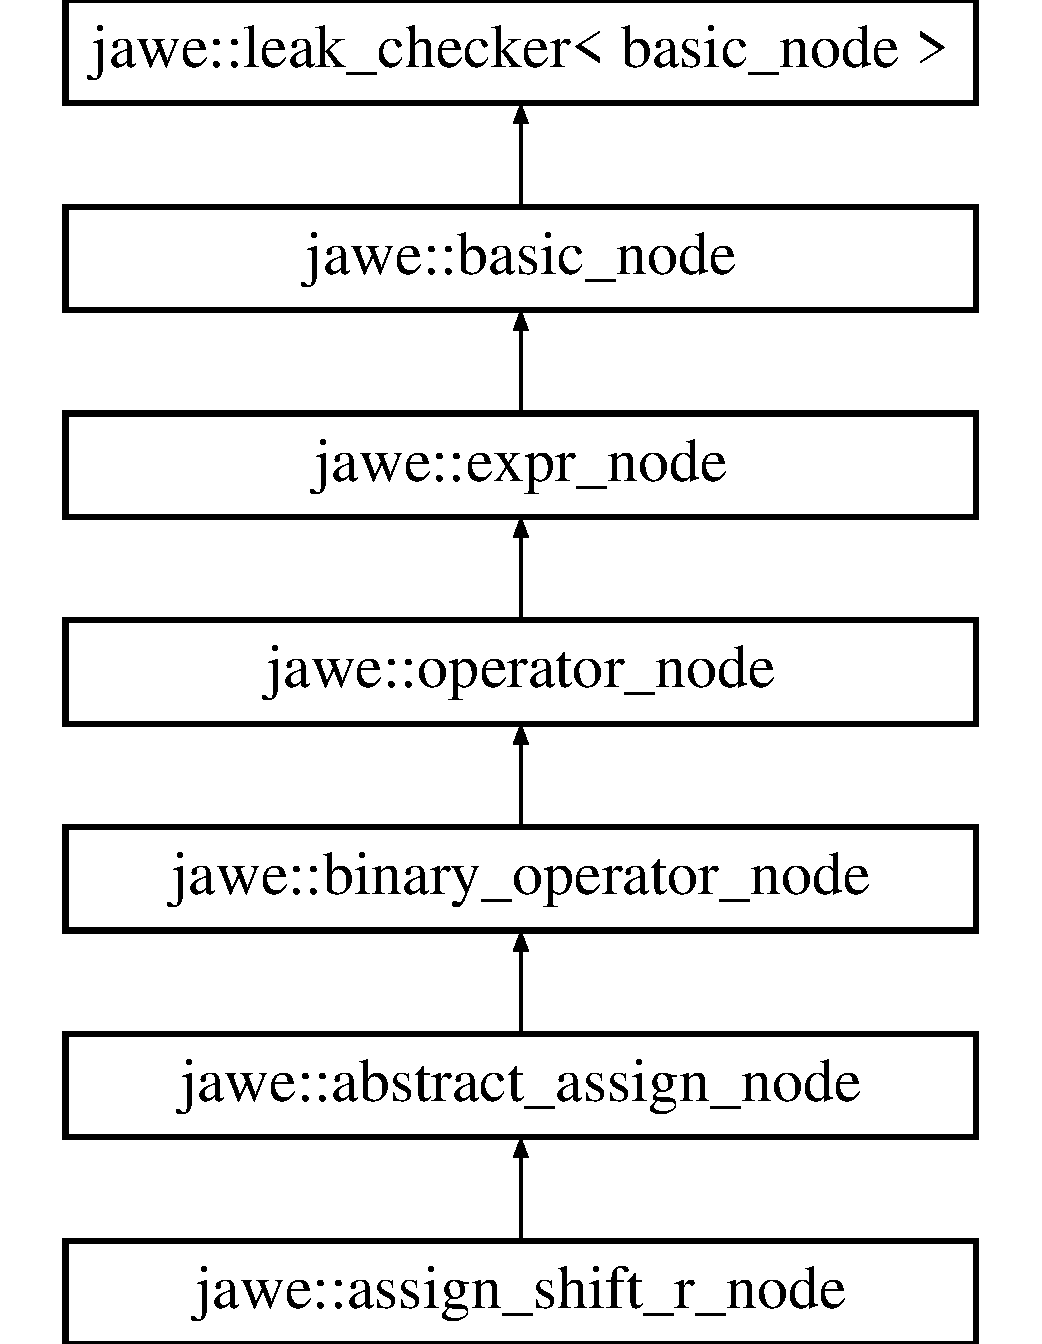
\includegraphics[height=7.000000cm]{classjawe_1_1assign__shift__r__node}
\end{center}
\end{figure}
\subsection*{Public Member Functions}
\begin{DoxyCompactItemize}
\item 
\hyperlink{classjawe_1_1assign__shift__r__node_a9258e637ddc109a6b8709f3076716c8e}{assign\+\_\+shift\+\_\+r\+\_\+node} (const \hyperlink{namespacejawe_a3f307481d921b6cbb50cc8511fc2b544}{shared\+\_\+node} \&, const \hyperlink{namespacejawe_a3f307481d921b6cbb50cc8511fc2b544}{shared\+\_\+node} \&)
\end{DoxyCompactItemize}
\subsection*{Additional Inherited Members}


\subsection{Constructor \& Destructor Documentation}
\mbox{\Hypertarget{classjawe_1_1assign__shift__r__node_a9258e637ddc109a6b8709f3076716c8e}\label{classjawe_1_1assign__shift__r__node_a9258e637ddc109a6b8709f3076716c8e}} 
\index{jawe\+::assign\+\_\+shift\+\_\+r\+\_\+node@{jawe\+::assign\+\_\+shift\+\_\+r\+\_\+node}!assign\+\_\+shift\+\_\+r\+\_\+node@{assign\+\_\+shift\+\_\+r\+\_\+node}}
\index{assign\+\_\+shift\+\_\+r\+\_\+node@{assign\+\_\+shift\+\_\+r\+\_\+node}!jawe\+::assign\+\_\+shift\+\_\+r\+\_\+node@{jawe\+::assign\+\_\+shift\+\_\+r\+\_\+node}}
\subsubsection{\texorpdfstring{assign\+\_\+shift\+\_\+r\+\_\+node()}{assign\_shift\_r\_node()}}
{\footnotesize\ttfamily assign\+\_\+shift\+\_\+r\+\_\+node\+::assign\+\_\+shift\+\_\+r\+\_\+node (\begin{DoxyParamCaption}\item[{const \hyperlink{namespacejawe_a3f307481d921b6cbb50cc8511fc2b544}{shared\+\_\+node} \&}]{left,  }\item[{const \hyperlink{namespacejawe_a3f307481d921b6cbb50cc8511fc2b544}{shared\+\_\+node} \&}]{right }\end{DoxyParamCaption})}



The documentation for this class was generated from the following files\+:\begin{DoxyCompactItemize}
\item 
include/syntax/operators/\hyperlink{assign__shift__r__node_8hpp}{assign\+\_\+shift\+\_\+r\+\_\+node.\+hpp}\item 
src/syntax/operators/\hyperlink{assign__shift__r__node_8cpp}{assign\+\_\+shift\+\_\+r\+\_\+node.\+cpp}\end{DoxyCompactItemize}

\hypertarget{classjawe_1_1assign__shift__u__node}{}\section{jawe\+:\+:assign\+\_\+shift\+\_\+u\+\_\+node Class Reference}
\label{classjawe_1_1assign__shift__u__node}\index{jawe\+::assign\+\_\+shift\+\_\+u\+\_\+node@{jawe\+::assign\+\_\+shift\+\_\+u\+\_\+node}}


{\ttfamily \#include $<$assign\+\_\+shift\+\_\+u\+\_\+node.\+hpp$>$}

Inheritance diagram for jawe\+:\+:assign\+\_\+shift\+\_\+u\+\_\+node\+:\begin{figure}[H]
\begin{center}
\leavevmode
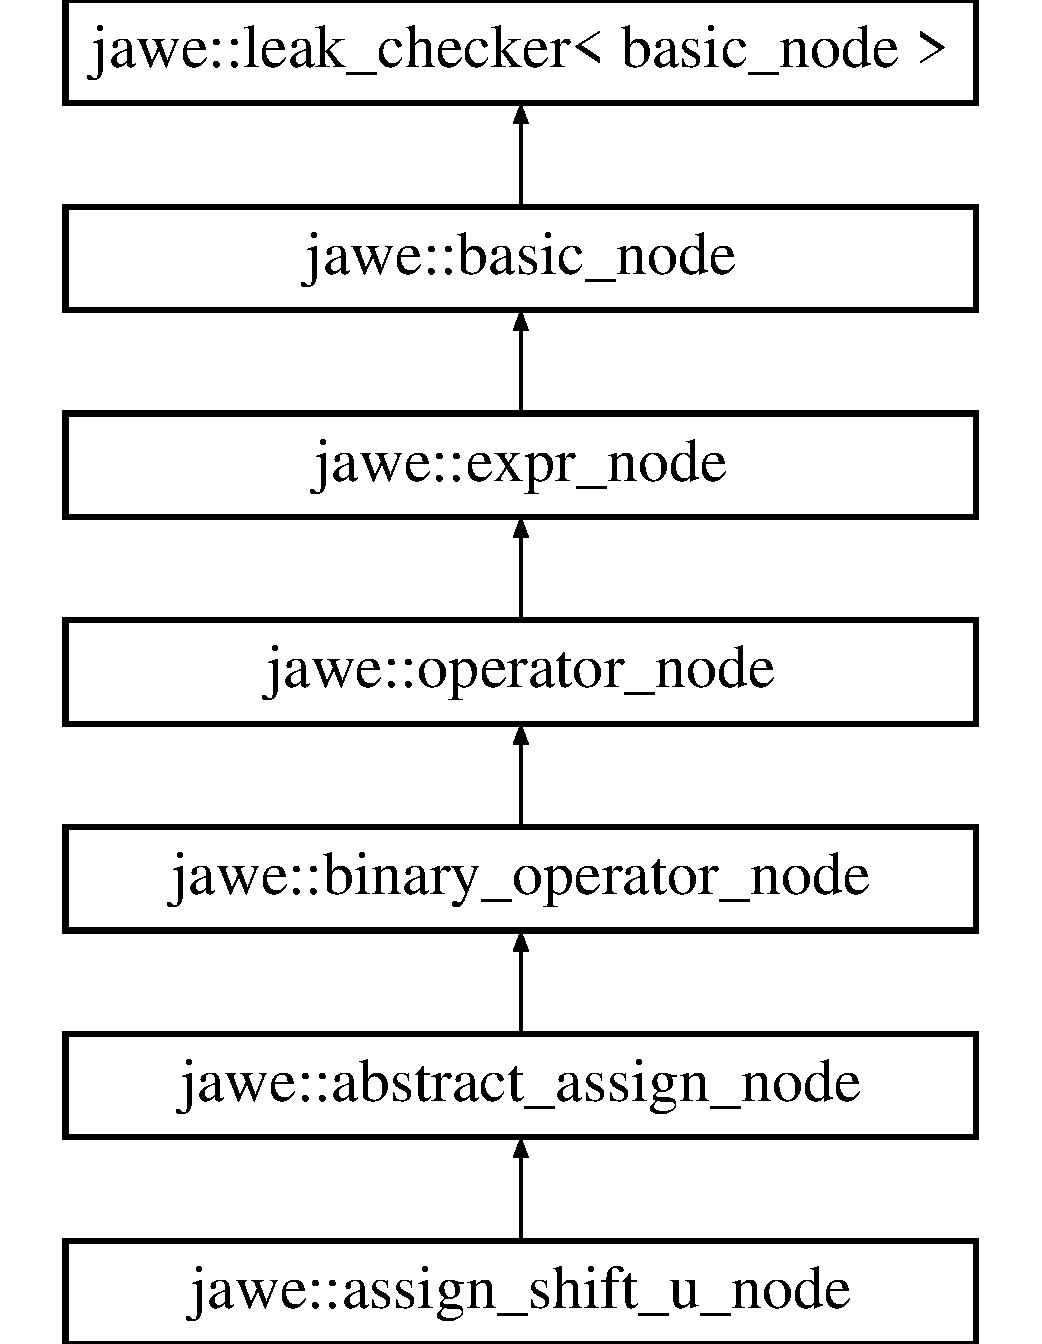
\includegraphics[height=7.000000cm]{classjawe_1_1assign__shift__u__node}
\end{center}
\end{figure}
\subsection*{Public Member Functions}
\begin{DoxyCompactItemize}
\item 
\hyperlink{classjawe_1_1assign__shift__u__node_a965641af110ec3272f699be47e06bc3c}{assign\+\_\+shift\+\_\+u\+\_\+node} (const \hyperlink{namespacejawe_a3f307481d921b6cbb50cc8511fc2b544}{shared\+\_\+node} \&, const \hyperlink{namespacejawe_a3f307481d921b6cbb50cc8511fc2b544}{shared\+\_\+node} \&)
\end{DoxyCompactItemize}
\subsection*{Additional Inherited Members}


\subsection{Constructor \& Destructor Documentation}
\mbox{\Hypertarget{classjawe_1_1assign__shift__u__node_a965641af110ec3272f699be47e06bc3c}\label{classjawe_1_1assign__shift__u__node_a965641af110ec3272f699be47e06bc3c}} 
\index{jawe\+::assign\+\_\+shift\+\_\+u\+\_\+node@{jawe\+::assign\+\_\+shift\+\_\+u\+\_\+node}!assign\+\_\+shift\+\_\+u\+\_\+node@{assign\+\_\+shift\+\_\+u\+\_\+node}}
\index{assign\+\_\+shift\+\_\+u\+\_\+node@{assign\+\_\+shift\+\_\+u\+\_\+node}!jawe\+::assign\+\_\+shift\+\_\+u\+\_\+node@{jawe\+::assign\+\_\+shift\+\_\+u\+\_\+node}}
\subsubsection{\texorpdfstring{assign\+\_\+shift\+\_\+u\+\_\+node()}{assign\_shift\_u\_node()}}
{\footnotesize\ttfamily assign\+\_\+shift\+\_\+u\+\_\+node\+::assign\+\_\+shift\+\_\+u\+\_\+node (\begin{DoxyParamCaption}\item[{const \hyperlink{namespacejawe_a3f307481d921b6cbb50cc8511fc2b544}{shared\+\_\+node} \&}]{left,  }\item[{const \hyperlink{namespacejawe_a3f307481d921b6cbb50cc8511fc2b544}{shared\+\_\+node} \&}]{right }\end{DoxyParamCaption})}



The documentation for this class was generated from the following files\+:\begin{DoxyCompactItemize}
\item 
include/syntax/operators/\hyperlink{assign__shift__u__node_8hpp}{assign\+\_\+shift\+\_\+u\+\_\+node.\+hpp}\item 
src/syntax/operators/\hyperlink{assign__shift__u__node_8cpp}{assign\+\_\+shift\+\_\+u\+\_\+node.\+cpp}\end{DoxyCompactItemize}

\hypertarget{classjawe_1_1basic__node}{}\section{jawe\+:\+:basic\+\_\+node Class Reference}
\label{classjawe_1_1basic__node}\index{jawe\+::basic\+\_\+node@{jawe\+::basic\+\_\+node}}


{\ttfamily \#include $<$shared\+\_\+node.\+hpp$>$}

Inheritance diagram for jawe\+:\+:basic\+\_\+node\+:\begin{figure}[H]
\begin{center}
\leavevmode
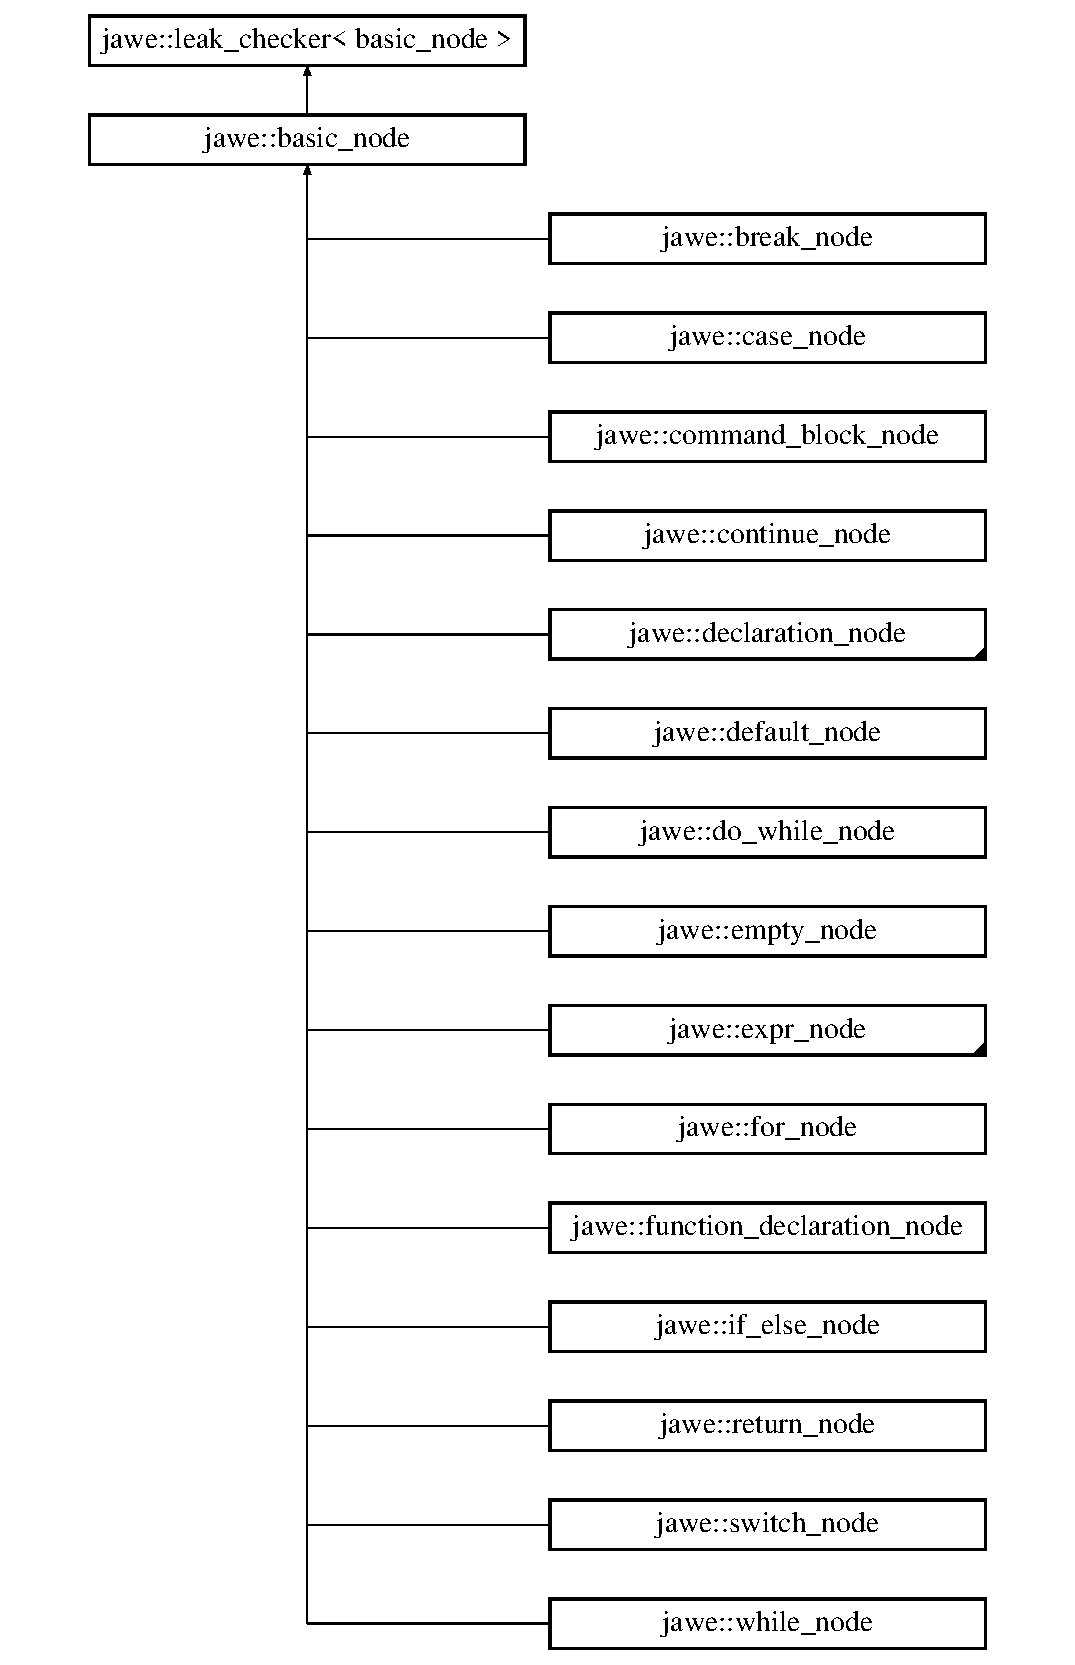
\includegraphics[height=12.000000cm]{classjawe_1_1basic__node}
\end{center}
\end{figure}
\subsection*{Public Member Functions}
\begin{DoxyCompactItemize}
\item 
std\+::string \hyperlink{classjawe_1_1basic__node_a06751766a924d6537794e8ff8e9958ff}{get\+\_\+symbol} () const
\item 
std\+::string \hyperlink{classjawe_1_1basic__node_a43ed68a61c23f89726070285f89245f5}{memory\+\_\+address} () const
\item 
int \hyperlink{classjawe_1_1basic__node_ac250c6262191048581228b8bba6eaebe}{get\+\_\+row} () const
\item 
int \hyperlink{classjawe_1_1basic__node_aafc0d609d65c9b16381d567bd7174c89}{get\+\_\+column} () const
\end{DoxyCompactItemize}
\subsection*{Protected Member Functions}
\begin{DoxyCompactItemize}
\item 
\hyperlink{classjawe_1_1basic__node_a2779d04e09d128b926171d1d543508d9}{basic\+\_\+node} (std\+::string)
\end{DoxyCompactItemize}
\subsection*{Private Attributes}
\begin{DoxyCompactItemize}
\item 
std\+::string \hyperlink{classjawe_1_1basic__node_ac6baed9e8bc01d8b953c1c42b8710057}{m\+\_\+symbol}
\item 
int \hyperlink{classjawe_1_1basic__node_ace1b7e8628dc9ac0b2562c6e2425d237}{m\+\_\+row}
\item 
int \hyperlink{classjawe_1_1basic__node_a219419e1836ea0af56c68aa8e026b0c6}{m\+\_\+column}
\end{DoxyCompactItemize}
\subsection*{Additional Inherited Members}


\subsection{Constructor \& Destructor Documentation}
\mbox{\Hypertarget{classjawe_1_1basic__node_a2779d04e09d128b926171d1d543508d9}\label{classjawe_1_1basic__node_a2779d04e09d128b926171d1d543508d9}} 
\index{jawe\+::basic\+\_\+node@{jawe\+::basic\+\_\+node}!basic\+\_\+node@{basic\+\_\+node}}
\index{basic\+\_\+node@{basic\+\_\+node}!jawe\+::basic\+\_\+node@{jawe\+::basic\+\_\+node}}
\subsubsection{\texorpdfstring{basic\+\_\+node()}{basic\_node()}}
{\footnotesize\ttfamily basic\+\_\+node\+::basic\+\_\+node (\begin{DoxyParamCaption}\item[{std\+::string}]{symbol }\end{DoxyParamCaption})\hspace{0.3cm}{\ttfamily [protected]}}



\subsection{Member Function Documentation}
\mbox{\Hypertarget{classjawe_1_1basic__node_aafc0d609d65c9b16381d567bd7174c89}\label{classjawe_1_1basic__node_aafc0d609d65c9b16381d567bd7174c89}} 
\index{jawe\+::basic\+\_\+node@{jawe\+::basic\+\_\+node}!get\+\_\+column@{get\+\_\+column}}
\index{get\+\_\+column@{get\+\_\+column}!jawe\+::basic\+\_\+node@{jawe\+::basic\+\_\+node}}
\subsubsection{\texorpdfstring{get\+\_\+column()}{get\_column()}}
{\footnotesize\ttfamily int basic\+\_\+node\+::get\+\_\+column (\begin{DoxyParamCaption}{ }\end{DoxyParamCaption}) const}

\mbox{\Hypertarget{classjawe_1_1basic__node_ac250c6262191048581228b8bba6eaebe}\label{classjawe_1_1basic__node_ac250c6262191048581228b8bba6eaebe}} 
\index{jawe\+::basic\+\_\+node@{jawe\+::basic\+\_\+node}!get\+\_\+row@{get\+\_\+row}}
\index{get\+\_\+row@{get\+\_\+row}!jawe\+::basic\+\_\+node@{jawe\+::basic\+\_\+node}}
\subsubsection{\texorpdfstring{get\+\_\+row()}{get\_row()}}
{\footnotesize\ttfamily int basic\+\_\+node\+::get\+\_\+row (\begin{DoxyParamCaption}{ }\end{DoxyParamCaption}) const}

\mbox{\Hypertarget{classjawe_1_1basic__node_a06751766a924d6537794e8ff8e9958ff}\label{classjawe_1_1basic__node_a06751766a924d6537794e8ff8e9958ff}} 
\index{jawe\+::basic\+\_\+node@{jawe\+::basic\+\_\+node}!get\+\_\+symbol@{get\+\_\+symbol}}
\index{get\+\_\+symbol@{get\+\_\+symbol}!jawe\+::basic\+\_\+node@{jawe\+::basic\+\_\+node}}
\subsubsection{\texorpdfstring{get\+\_\+symbol()}{get\_symbol()}}
{\footnotesize\ttfamily std\+::string basic\+\_\+node\+::get\+\_\+symbol (\begin{DoxyParamCaption}{ }\end{DoxyParamCaption}) const}

\mbox{\Hypertarget{classjawe_1_1basic__node_a43ed68a61c23f89726070285f89245f5}\label{classjawe_1_1basic__node_a43ed68a61c23f89726070285f89245f5}} 
\index{jawe\+::basic\+\_\+node@{jawe\+::basic\+\_\+node}!memory\+\_\+address@{memory\+\_\+address}}
\index{memory\+\_\+address@{memory\+\_\+address}!jawe\+::basic\+\_\+node@{jawe\+::basic\+\_\+node}}
\subsubsection{\texorpdfstring{memory\+\_\+address()}{memory\_address()}}
{\footnotesize\ttfamily std\+::string basic\+\_\+node\+::memory\+\_\+address (\begin{DoxyParamCaption}{ }\end{DoxyParamCaption}) const}



\subsection{Member Data Documentation}
\mbox{\Hypertarget{classjawe_1_1basic__node_a219419e1836ea0af56c68aa8e026b0c6}\label{classjawe_1_1basic__node_a219419e1836ea0af56c68aa8e026b0c6}} 
\index{jawe\+::basic\+\_\+node@{jawe\+::basic\+\_\+node}!m\+\_\+column@{m\+\_\+column}}
\index{m\+\_\+column@{m\+\_\+column}!jawe\+::basic\+\_\+node@{jawe\+::basic\+\_\+node}}
\subsubsection{\texorpdfstring{m\+\_\+column}{m\_column}}
{\footnotesize\ttfamily int jawe\+::basic\+\_\+node\+::m\+\_\+column\hspace{0.3cm}{\ttfamily [private]}}

\mbox{\Hypertarget{classjawe_1_1basic__node_ace1b7e8628dc9ac0b2562c6e2425d237}\label{classjawe_1_1basic__node_ace1b7e8628dc9ac0b2562c6e2425d237}} 
\index{jawe\+::basic\+\_\+node@{jawe\+::basic\+\_\+node}!m\+\_\+row@{m\+\_\+row}}
\index{m\+\_\+row@{m\+\_\+row}!jawe\+::basic\+\_\+node@{jawe\+::basic\+\_\+node}}
\subsubsection{\texorpdfstring{m\+\_\+row}{m\_row}}
{\footnotesize\ttfamily int jawe\+::basic\+\_\+node\+::m\+\_\+row\hspace{0.3cm}{\ttfamily [private]}}

\mbox{\Hypertarget{classjawe_1_1basic__node_ac6baed9e8bc01d8b953c1c42b8710057}\label{classjawe_1_1basic__node_ac6baed9e8bc01d8b953c1c42b8710057}} 
\index{jawe\+::basic\+\_\+node@{jawe\+::basic\+\_\+node}!m\+\_\+symbol@{m\+\_\+symbol}}
\index{m\+\_\+symbol@{m\+\_\+symbol}!jawe\+::basic\+\_\+node@{jawe\+::basic\+\_\+node}}
\subsubsection{\texorpdfstring{m\+\_\+symbol}{m\_symbol}}
{\footnotesize\ttfamily std\+::string jawe\+::basic\+\_\+node\+::m\+\_\+symbol\hspace{0.3cm}{\ttfamily [private]}}



The documentation for this class was generated from the following files\+:\begin{DoxyCompactItemize}
\item 
include/syntax/abstract/\hyperlink{shared__node_8hpp}{shared\+\_\+node.\+hpp}\item 
src/syntax/abstract/\hyperlink{shared__node_8cpp}{shared\+\_\+node.\+cpp}\end{DoxyCompactItemize}

\hypertarget{classbasic__operation}{}\section{basic\+\_\+operation Class Reference}
\label{classbasic__operation}\index{basic\+\_\+operation@{basic\+\_\+operation}}


{\ttfamily \#include $<$basic\+\_\+operation.\+hpp$>$}

Inheritance diagram for basic\+\_\+operation\+:\begin{figure}[H]
\begin{center}
\leavevmode
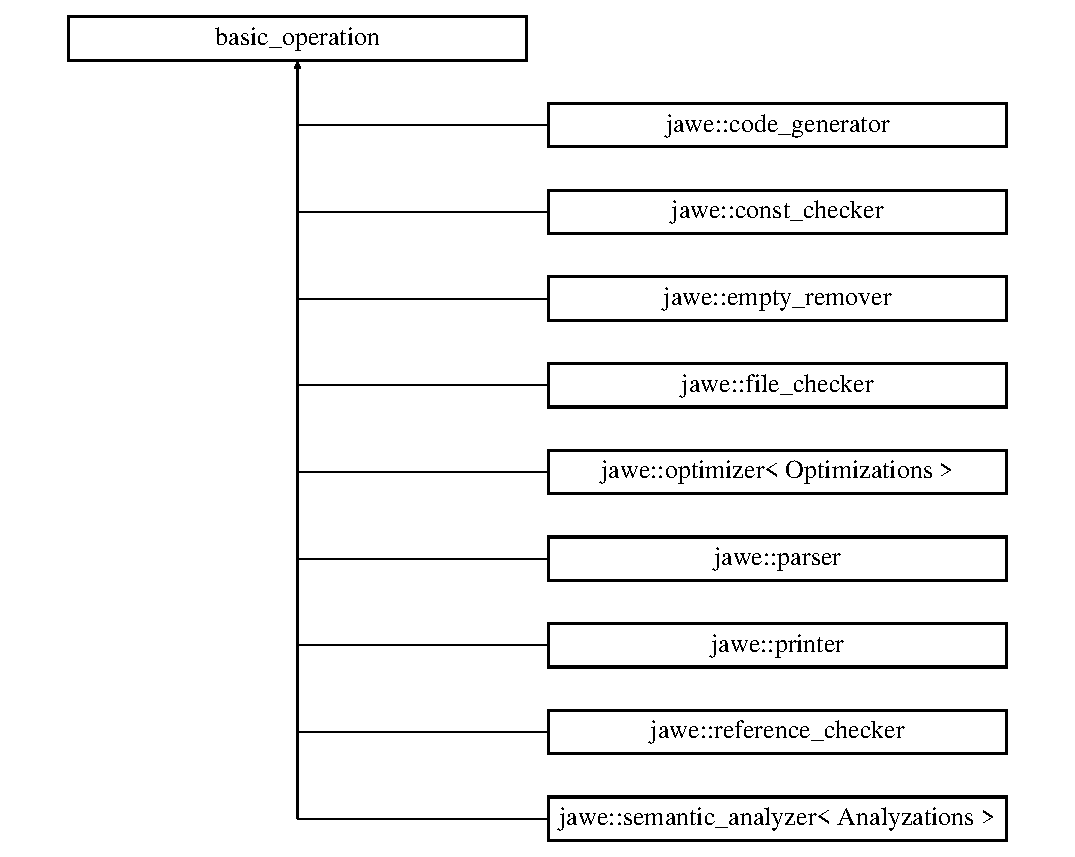
\includegraphics[height=10.000000cm]{classbasic__operation}
\end{center}
\end{figure}


The documentation for this class was generated from the following file\+:\begin{DoxyCompactItemize}
\item 
include/operations/\hyperlink{basic__operation_8hpp}{basic\+\_\+operation.\+hpp}\end{DoxyCompactItemize}

\hypertarget{classjawe_1_1basic__transformation}{}\section{jawe\+:\+:basic\+\_\+transformation Class Reference}
\label{classjawe_1_1basic__transformation}\index{jawe\+::basic\+\_\+transformation@{jawe\+::basic\+\_\+transformation}}


{\ttfamily \#include $<$basic\+\_\+transformation.\+hpp$>$}

Inheritance diagram for jawe\+:\+:basic\+\_\+transformation\+:\begin{figure}[H]
\begin{center}
\leavevmode
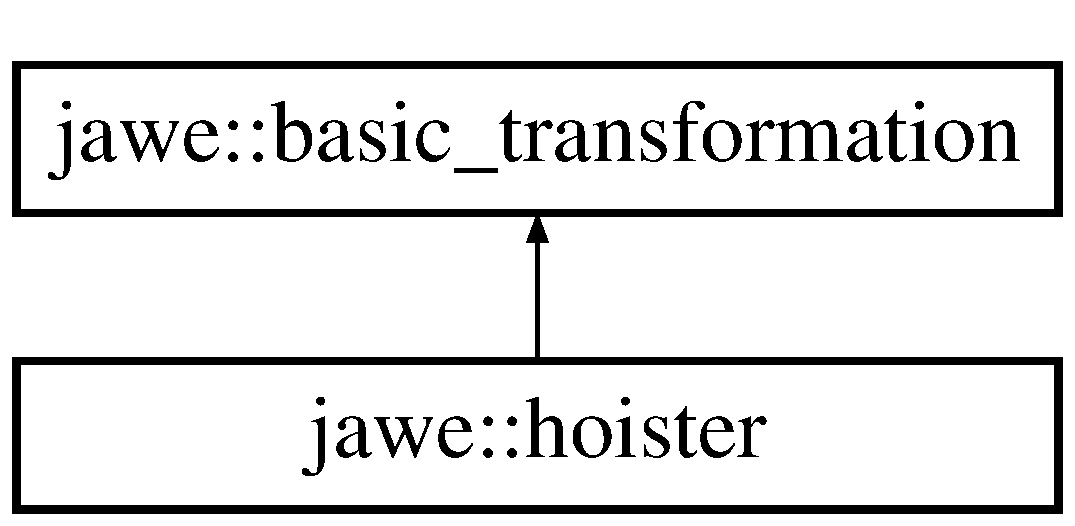
\includegraphics[height=2.000000cm]{classjawe_1_1basic__transformation}
\end{center}
\end{figure}
\subsection*{Public Member Functions}
\begin{DoxyCompactItemize}
\item 
void \hyperlink{classjawe_1_1basic__transformation_a40c48c034ae20b1f2624bc33158e33e0}{run} () const
\end{DoxyCompactItemize}


\subsection{Member Function Documentation}
\mbox{\Hypertarget{classjawe_1_1basic__transformation_a40c48c034ae20b1f2624bc33158e33e0}\label{classjawe_1_1basic__transformation_a40c48c034ae20b1f2624bc33158e33e0}} 
\index{jawe\+::basic\+\_\+transformation@{jawe\+::basic\+\_\+transformation}!run@{run}}
\index{run@{run}!jawe\+::basic\+\_\+transformation@{jawe\+::basic\+\_\+transformation}}
\subsubsection{\texorpdfstring{run()}{run()}}
{\footnotesize\ttfamily void jawe\+::basic\+\_\+transformation\+::run (\begin{DoxyParamCaption}{ }\end{DoxyParamCaption}) const}



The documentation for this class was generated from the following file\+:\begin{DoxyCompactItemize}
\item 
include/transformations/\hyperlink{basic__transformation_8hpp}{basic\+\_\+transformation.\+hpp}\end{DoxyCompactItemize}

\hypertarget{classjawe_1_1binary__operator__node}{}\section{jawe\+:\+:binary\+\_\+operator\+\_\+node Class Reference}
\label{classjawe_1_1binary__operator__node}\index{jawe\+::binary\+\_\+operator\+\_\+node@{jawe\+::binary\+\_\+operator\+\_\+node}}


{\ttfamily \#include $<$binary\+\_\+operator\+\_\+node.\+hpp$>$}

Inheritance diagram for jawe\+:\+:binary\+\_\+operator\+\_\+node\+:\begin{figure}[H]
\begin{center}
\leavevmode
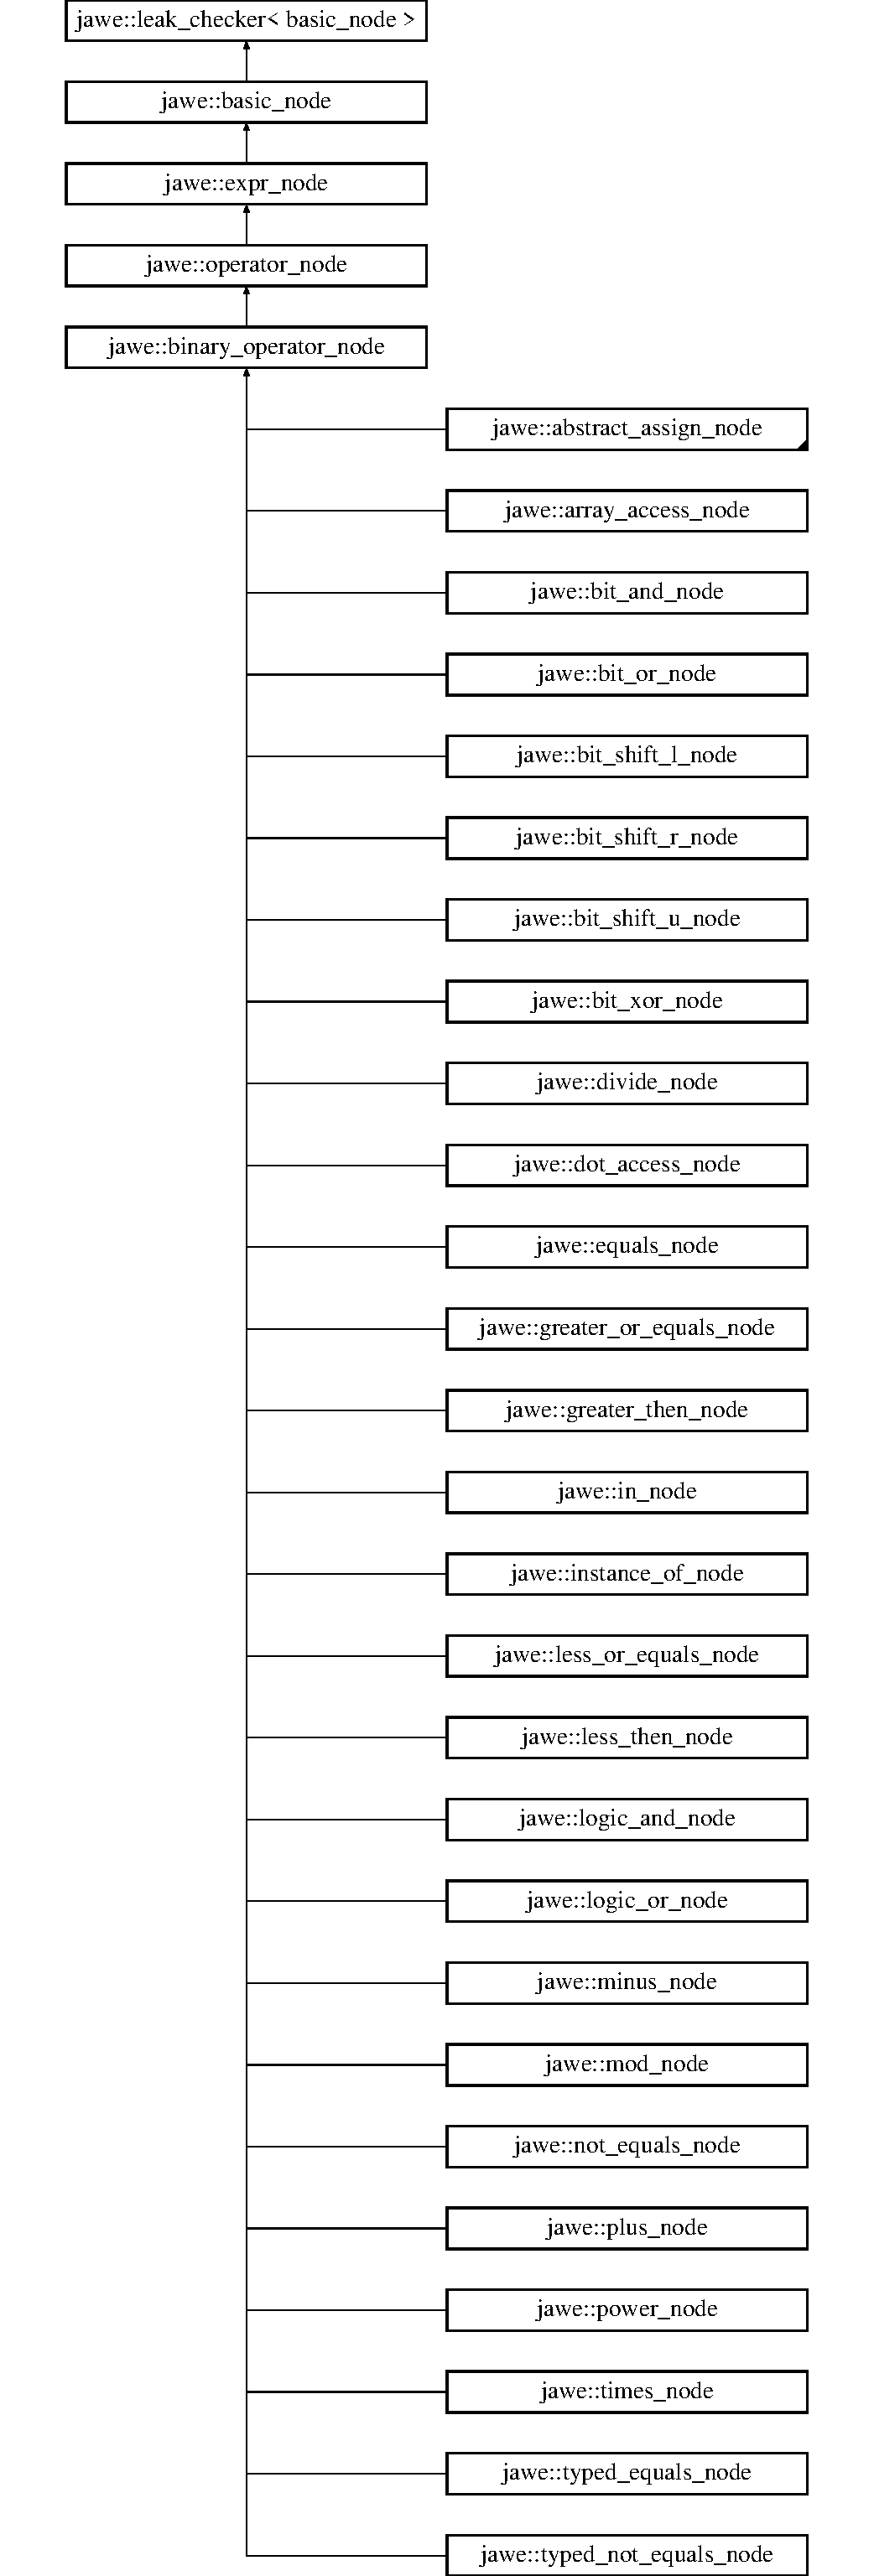
\includegraphics[height=12.000000cm]{classjawe_1_1binary__operator__node}
\end{center}
\end{figure}
\subsection*{Public Member Functions}
\begin{DoxyCompactItemize}
\item 
\hyperlink{classjawe_1_1binary__operator__node_a38237c97b9f17f6ba32b7e18c4795a99}{binary\+\_\+operator\+\_\+node} (const \hyperlink{namespacejawe_a3f307481d921b6cbb50cc8511fc2b544}{shared\+\_\+node} \&, const \hyperlink{namespacejawe_a3f307481d921b6cbb50cc8511fc2b544}{shared\+\_\+node} \&, std\+::string)
\item 
\hyperlink{namespacejawe_a3f307481d921b6cbb50cc8511fc2b544}{shared\+\_\+node} \hyperlink{classjawe_1_1binary__operator__node_a573ef1c5736807a686ae25dcd9e0d241}{get\+\_\+left} () const
\item 
\hyperlink{namespacejawe_a3f307481d921b6cbb50cc8511fc2b544}{shared\+\_\+node} \hyperlink{classjawe_1_1binary__operator__node_a1294c8994976f2411d1382a240136104}{get\+\_\+right} () const
\end{DoxyCompactItemize}
\subsection*{Private Attributes}
\begin{DoxyCompactItemize}
\item 
\hyperlink{namespacejawe_a3f307481d921b6cbb50cc8511fc2b544}{shared\+\_\+node} \hyperlink{classjawe_1_1binary__operator__node_aadc5aa4653bff38e1f4f0110a36de63b}{m\+\_\+left}
\item 
\hyperlink{namespacejawe_a3f307481d921b6cbb50cc8511fc2b544}{shared\+\_\+node} \hyperlink{classjawe_1_1binary__operator__node_add4099a75e39ab3931d71b3d6e1032c8}{m\+\_\+right}
\end{DoxyCompactItemize}
\subsection*{Additional Inherited Members}


\subsection{Constructor \& Destructor Documentation}
\mbox{\Hypertarget{classjawe_1_1binary__operator__node_a38237c97b9f17f6ba32b7e18c4795a99}\label{classjawe_1_1binary__operator__node_a38237c97b9f17f6ba32b7e18c4795a99}} 
\index{jawe\+::binary\+\_\+operator\+\_\+node@{jawe\+::binary\+\_\+operator\+\_\+node}!binary\+\_\+operator\+\_\+node@{binary\+\_\+operator\+\_\+node}}
\index{binary\+\_\+operator\+\_\+node@{binary\+\_\+operator\+\_\+node}!jawe\+::binary\+\_\+operator\+\_\+node@{jawe\+::binary\+\_\+operator\+\_\+node}}
\subsubsection{\texorpdfstring{binary\+\_\+operator\+\_\+node()}{binary\_operator\_node()}}
{\footnotesize\ttfamily binary\+\_\+operator\+\_\+node\+::binary\+\_\+operator\+\_\+node (\begin{DoxyParamCaption}\item[{const \hyperlink{namespacejawe_a3f307481d921b6cbb50cc8511fc2b544}{shared\+\_\+node} \&}]{left,  }\item[{const \hyperlink{namespacejawe_a3f307481d921b6cbb50cc8511fc2b544}{shared\+\_\+node} \&}]{right,  }\item[{std\+::string}]{symbol }\end{DoxyParamCaption})}



\subsection{Member Function Documentation}
\mbox{\Hypertarget{classjawe_1_1binary__operator__node_a573ef1c5736807a686ae25dcd9e0d241}\label{classjawe_1_1binary__operator__node_a573ef1c5736807a686ae25dcd9e0d241}} 
\index{jawe\+::binary\+\_\+operator\+\_\+node@{jawe\+::binary\+\_\+operator\+\_\+node}!get\+\_\+left@{get\+\_\+left}}
\index{get\+\_\+left@{get\+\_\+left}!jawe\+::binary\+\_\+operator\+\_\+node@{jawe\+::binary\+\_\+operator\+\_\+node}}
\subsubsection{\texorpdfstring{get\+\_\+left()}{get\_left()}}
{\footnotesize\ttfamily \hyperlink{namespacejawe_a3f307481d921b6cbb50cc8511fc2b544}{shared\+\_\+node} binary\+\_\+operator\+\_\+node\+::get\+\_\+left (\begin{DoxyParamCaption}{ }\end{DoxyParamCaption}) const}

\mbox{\Hypertarget{classjawe_1_1binary__operator__node_a1294c8994976f2411d1382a240136104}\label{classjawe_1_1binary__operator__node_a1294c8994976f2411d1382a240136104}} 
\index{jawe\+::binary\+\_\+operator\+\_\+node@{jawe\+::binary\+\_\+operator\+\_\+node}!get\+\_\+right@{get\+\_\+right}}
\index{get\+\_\+right@{get\+\_\+right}!jawe\+::binary\+\_\+operator\+\_\+node@{jawe\+::binary\+\_\+operator\+\_\+node}}
\subsubsection{\texorpdfstring{get\+\_\+right()}{get\_right()}}
{\footnotesize\ttfamily \hyperlink{namespacejawe_a3f307481d921b6cbb50cc8511fc2b544}{shared\+\_\+node} binary\+\_\+operator\+\_\+node\+::get\+\_\+right (\begin{DoxyParamCaption}{ }\end{DoxyParamCaption}) const}



\subsection{Member Data Documentation}
\mbox{\Hypertarget{classjawe_1_1binary__operator__node_aadc5aa4653bff38e1f4f0110a36de63b}\label{classjawe_1_1binary__operator__node_aadc5aa4653bff38e1f4f0110a36de63b}} 
\index{jawe\+::binary\+\_\+operator\+\_\+node@{jawe\+::binary\+\_\+operator\+\_\+node}!m\+\_\+left@{m\+\_\+left}}
\index{m\+\_\+left@{m\+\_\+left}!jawe\+::binary\+\_\+operator\+\_\+node@{jawe\+::binary\+\_\+operator\+\_\+node}}
\subsubsection{\texorpdfstring{m\+\_\+left}{m\_left}}
{\footnotesize\ttfamily \hyperlink{namespacejawe_a3f307481d921b6cbb50cc8511fc2b544}{shared\+\_\+node} jawe\+::binary\+\_\+operator\+\_\+node\+::m\+\_\+left\hspace{0.3cm}{\ttfamily [private]}}

\mbox{\Hypertarget{classjawe_1_1binary__operator__node_add4099a75e39ab3931d71b3d6e1032c8}\label{classjawe_1_1binary__operator__node_add4099a75e39ab3931d71b3d6e1032c8}} 
\index{jawe\+::binary\+\_\+operator\+\_\+node@{jawe\+::binary\+\_\+operator\+\_\+node}!m\+\_\+right@{m\+\_\+right}}
\index{m\+\_\+right@{m\+\_\+right}!jawe\+::binary\+\_\+operator\+\_\+node@{jawe\+::binary\+\_\+operator\+\_\+node}}
\subsubsection{\texorpdfstring{m\+\_\+right}{m\_right}}
{\footnotesize\ttfamily \hyperlink{namespacejawe_a3f307481d921b6cbb50cc8511fc2b544}{shared\+\_\+node} jawe\+::binary\+\_\+operator\+\_\+node\+::m\+\_\+right\hspace{0.3cm}{\ttfamily [private]}}



The documentation for this class was generated from the following files\+:\begin{DoxyCompactItemize}
\item 
include/syntax/operators/\hyperlink{binary__operator__node_8hpp}{binary\+\_\+operator\+\_\+node.\+hpp}\item 
src/syntax/operators/\hyperlink{binary__operator__node_8cpp}{binary\+\_\+operator\+\_\+node.\+cpp}\end{DoxyCompactItemize}

\hypertarget{classjawe_1_1bit__and__node}{}\section{jawe\+:\+:bit\+\_\+and\+\_\+node Class Reference}
\label{classjawe_1_1bit__and__node}\index{jawe\+::bit\+\_\+and\+\_\+node@{jawe\+::bit\+\_\+and\+\_\+node}}


{\ttfamily \#include $<$bit\+\_\+and\+\_\+node.\+hpp$>$}

Inheritance diagram for jawe\+:\+:bit\+\_\+and\+\_\+node\+:\begin{figure}[H]
\begin{center}
\leavevmode
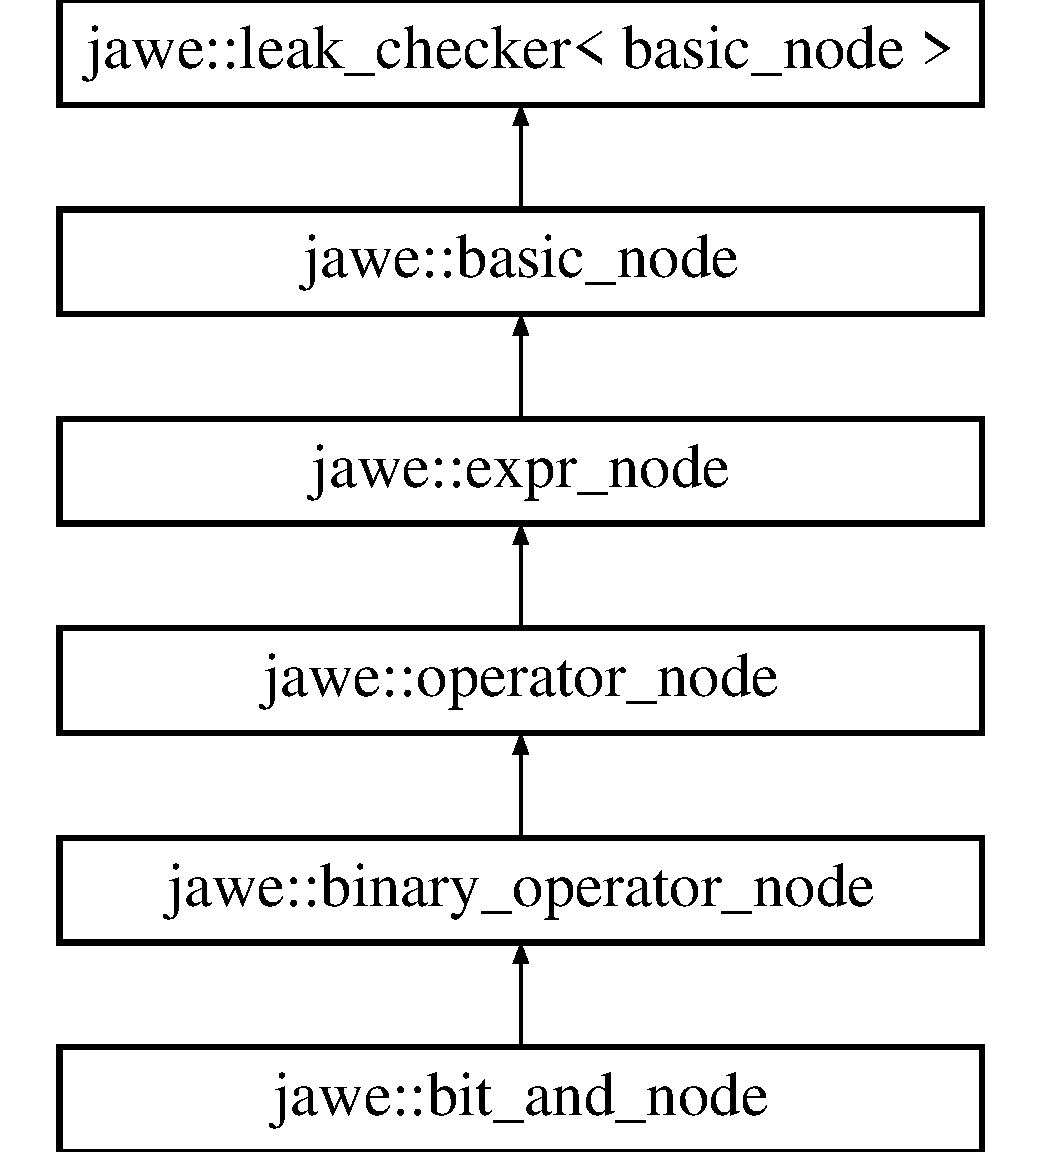
\includegraphics[height=6.000000cm]{classjawe_1_1bit__and__node}
\end{center}
\end{figure}
\subsection*{Public Member Functions}
\begin{DoxyCompactItemize}
\item 
\hyperlink{classjawe_1_1bit__and__node_a2e3a28111fa7dd0ec8d209d5211fec99}{bit\+\_\+and\+\_\+node} (const \hyperlink{namespacejawe_a3f307481d921b6cbb50cc8511fc2b544}{shared\+\_\+node} \&, const \hyperlink{namespacejawe_a3f307481d921b6cbb50cc8511fc2b544}{shared\+\_\+node} \&)
\end{DoxyCompactItemize}
\subsection*{Additional Inherited Members}


\subsection{Constructor \& Destructor Documentation}
\mbox{\Hypertarget{classjawe_1_1bit__and__node_a2e3a28111fa7dd0ec8d209d5211fec99}\label{classjawe_1_1bit__and__node_a2e3a28111fa7dd0ec8d209d5211fec99}} 
\index{jawe\+::bit\+\_\+and\+\_\+node@{jawe\+::bit\+\_\+and\+\_\+node}!bit\+\_\+and\+\_\+node@{bit\+\_\+and\+\_\+node}}
\index{bit\+\_\+and\+\_\+node@{bit\+\_\+and\+\_\+node}!jawe\+::bit\+\_\+and\+\_\+node@{jawe\+::bit\+\_\+and\+\_\+node}}
\subsubsection{\texorpdfstring{bit\+\_\+and\+\_\+node()}{bit\_and\_node()}}
{\footnotesize\ttfamily bit\+\_\+and\+\_\+node\+::bit\+\_\+and\+\_\+node (\begin{DoxyParamCaption}\item[{const \hyperlink{namespacejawe_a3f307481d921b6cbb50cc8511fc2b544}{shared\+\_\+node} \&}]{left,  }\item[{const \hyperlink{namespacejawe_a3f307481d921b6cbb50cc8511fc2b544}{shared\+\_\+node} \&}]{right }\end{DoxyParamCaption})}



The documentation for this class was generated from the following files\+:\begin{DoxyCompactItemize}
\item 
include/syntax/operators/\hyperlink{bit__and__node_8hpp}{bit\+\_\+and\+\_\+node.\+hpp}\item 
src/syntax/operators/\hyperlink{bit__and__node_8cpp}{bit\+\_\+and\+\_\+node.\+cpp}\end{DoxyCompactItemize}

\hypertarget{classjawe_1_1bit__not__node}{}\section{jawe\+:\+:bit\+\_\+not\+\_\+node Class Reference}
\label{classjawe_1_1bit__not__node}\index{jawe\+::bit\+\_\+not\+\_\+node@{jawe\+::bit\+\_\+not\+\_\+node}}


{\ttfamily \#include $<$bit\+\_\+not\+\_\+node.\+hpp$>$}

Inheritance diagram for jawe\+:\+:bit\+\_\+not\+\_\+node\+:\begin{figure}[H]
\begin{center}
\leavevmode
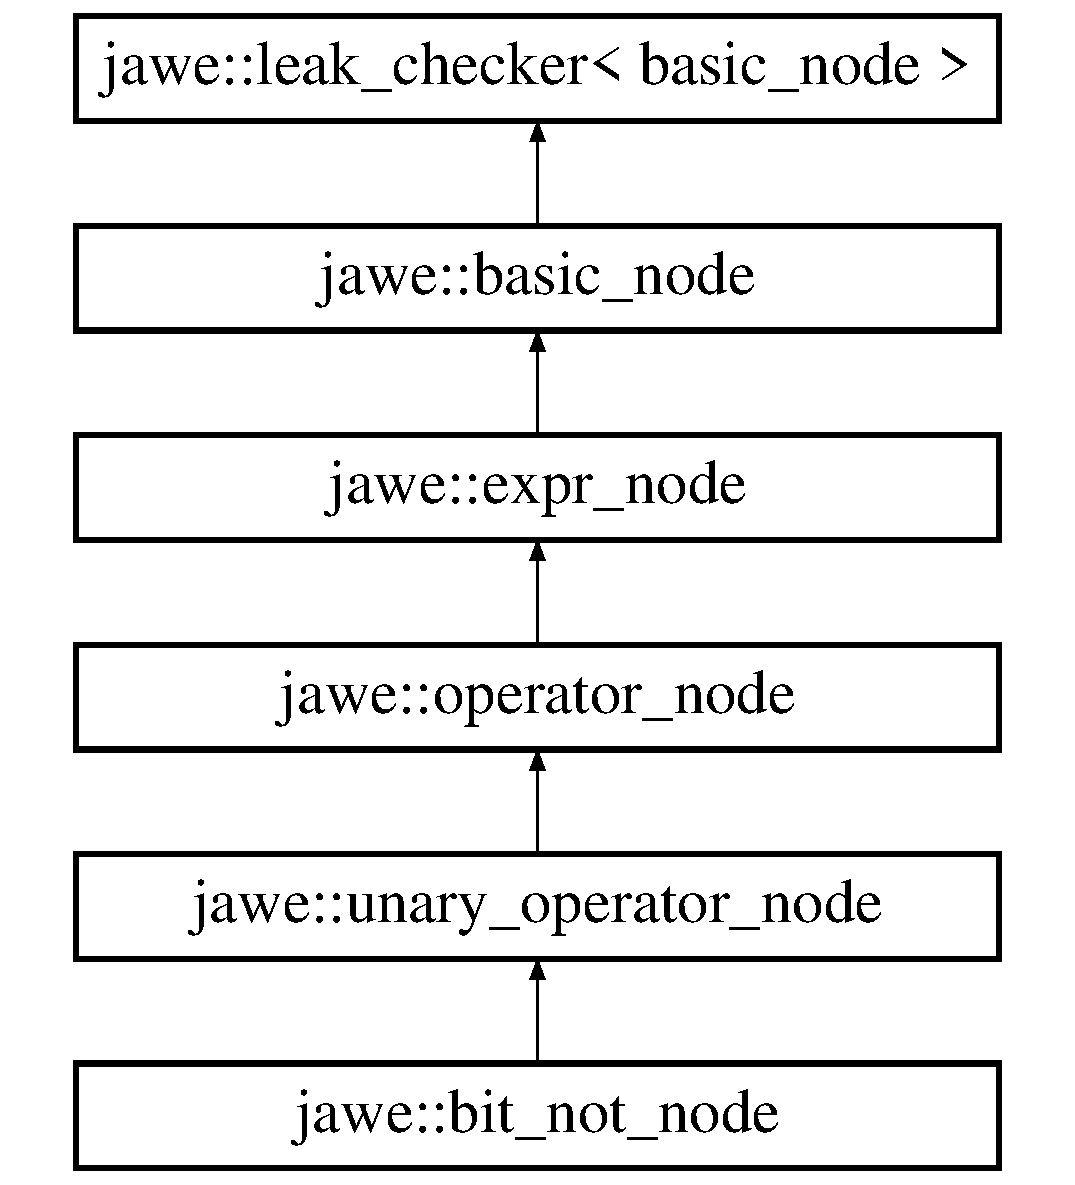
\includegraphics[height=6.000000cm]{classjawe_1_1bit__not__node}
\end{center}
\end{figure}
\subsection*{Public Member Functions}
\begin{DoxyCompactItemize}
\item 
\hyperlink{classjawe_1_1bit__not__node_a2d14c296ba805a6e47eedd9286e4d7d0}{bit\+\_\+not\+\_\+node} (const \hyperlink{namespacejawe_a3f307481d921b6cbb50cc8511fc2b544}{shared\+\_\+node} \&)
\end{DoxyCompactItemize}
\subsection*{Additional Inherited Members}


\subsection{Constructor \& Destructor Documentation}
\mbox{\Hypertarget{classjawe_1_1bit__not__node_a2d14c296ba805a6e47eedd9286e4d7d0}\label{classjawe_1_1bit__not__node_a2d14c296ba805a6e47eedd9286e4d7d0}} 
\index{jawe\+::bit\+\_\+not\+\_\+node@{jawe\+::bit\+\_\+not\+\_\+node}!bit\+\_\+not\+\_\+node@{bit\+\_\+not\+\_\+node}}
\index{bit\+\_\+not\+\_\+node@{bit\+\_\+not\+\_\+node}!jawe\+::bit\+\_\+not\+\_\+node@{jawe\+::bit\+\_\+not\+\_\+node}}
\subsubsection{\texorpdfstring{bit\+\_\+not\+\_\+node()}{bit\_not\_node()}}
{\footnotesize\ttfamily bit\+\_\+not\+\_\+node\+::bit\+\_\+not\+\_\+node (\begin{DoxyParamCaption}\item[{const \hyperlink{namespacejawe_a3f307481d921b6cbb50cc8511fc2b544}{shared\+\_\+node} \&}]{operand }\end{DoxyParamCaption})}



The documentation for this class was generated from the following files\+:\begin{DoxyCompactItemize}
\item 
include/syntax/operators/\hyperlink{bit__not__node_8hpp}{bit\+\_\+not\+\_\+node.\+hpp}\item 
src/syntax/operators/\hyperlink{bit__not__node_8cpp}{bit\+\_\+not\+\_\+node.\+cpp}\end{DoxyCompactItemize}

\hypertarget{classjawe_1_1bit__or__node}{}\section{jawe\+:\+:bit\+\_\+or\+\_\+node Class Reference}
\label{classjawe_1_1bit__or__node}\index{jawe\+::bit\+\_\+or\+\_\+node@{jawe\+::bit\+\_\+or\+\_\+node}}


{\ttfamily \#include $<$bit\+\_\+or\+\_\+node.\+hpp$>$}

Inheritance diagram for jawe\+:\+:bit\+\_\+or\+\_\+node\+:\begin{figure}[H]
\begin{center}
\leavevmode
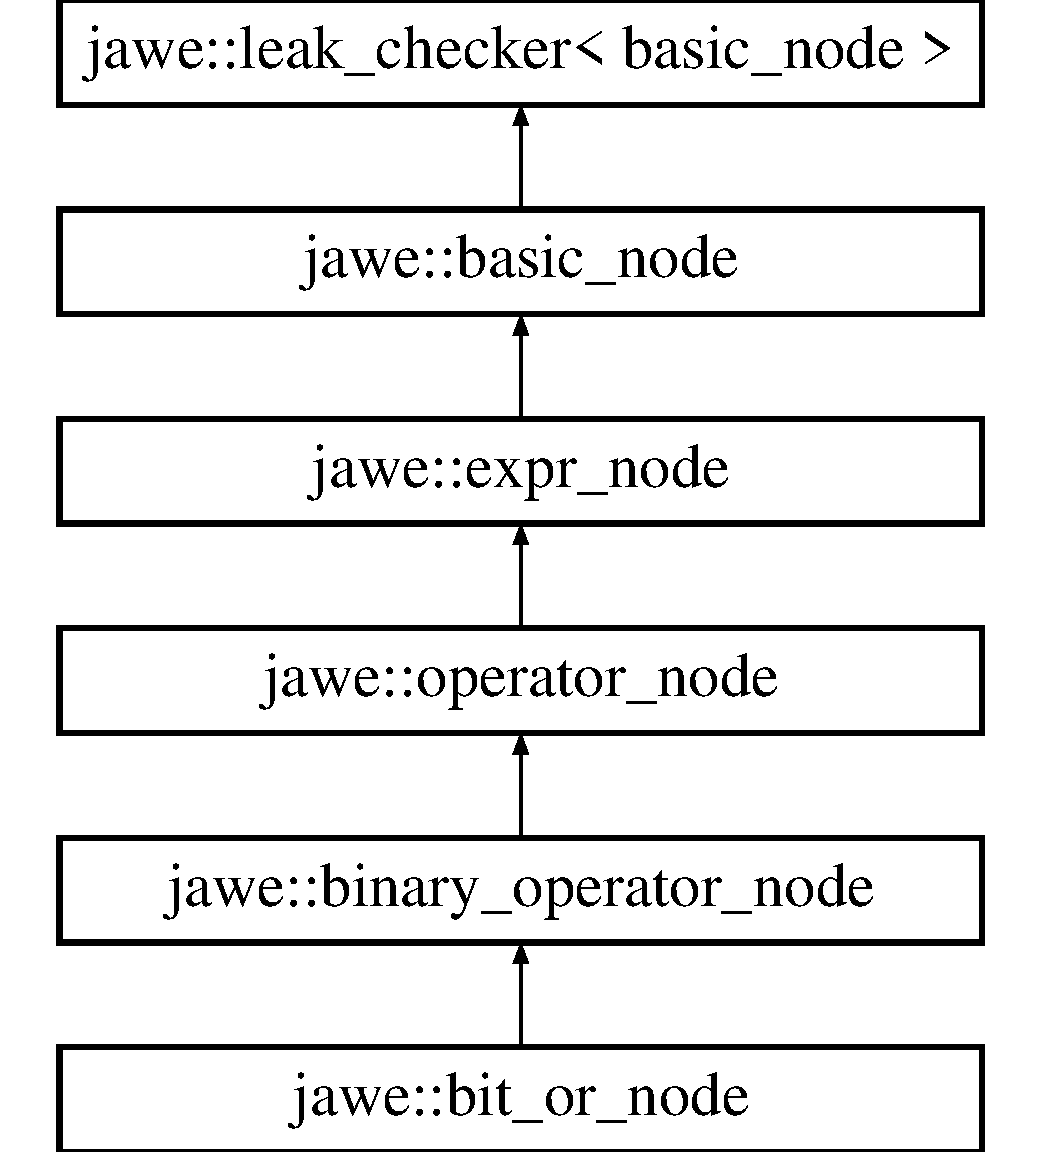
\includegraphics[height=6.000000cm]{classjawe_1_1bit__or__node}
\end{center}
\end{figure}
\subsection*{Public Member Functions}
\begin{DoxyCompactItemize}
\item 
\hyperlink{classjawe_1_1bit__or__node_ad1b739037f4d4dd0a69fffc88692e569}{bit\+\_\+or\+\_\+node} (const \hyperlink{namespacejawe_a3f307481d921b6cbb50cc8511fc2b544}{shared\+\_\+node} \&, const \hyperlink{namespacejawe_a3f307481d921b6cbb50cc8511fc2b544}{shared\+\_\+node} \&)
\end{DoxyCompactItemize}
\subsection*{Additional Inherited Members}


\subsection{Constructor \& Destructor Documentation}
\mbox{\Hypertarget{classjawe_1_1bit__or__node_ad1b739037f4d4dd0a69fffc88692e569}\label{classjawe_1_1bit__or__node_ad1b739037f4d4dd0a69fffc88692e569}} 
\index{jawe\+::bit\+\_\+or\+\_\+node@{jawe\+::bit\+\_\+or\+\_\+node}!bit\+\_\+or\+\_\+node@{bit\+\_\+or\+\_\+node}}
\index{bit\+\_\+or\+\_\+node@{bit\+\_\+or\+\_\+node}!jawe\+::bit\+\_\+or\+\_\+node@{jawe\+::bit\+\_\+or\+\_\+node}}
\subsubsection{\texorpdfstring{bit\+\_\+or\+\_\+node()}{bit\_or\_node()}}
{\footnotesize\ttfamily bit\+\_\+or\+\_\+node\+::bit\+\_\+or\+\_\+node (\begin{DoxyParamCaption}\item[{const \hyperlink{namespacejawe_a3f307481d921b6cbb50cc8511fc2b544}{shared\+\_\+node} \&}]{left,  }\item[{const \hyperlink{namespacejawe_a3f307481d921b6cbb50cc8511fc2b544}{shared\+\_\+node} \&}]{right }\end{DoxyParamCaption})}



The documentation for this class was generated from the following files\+:\begin{DoxyCompactItemize}
\item 
include/syntax/operators/\hyperlink{bit__or__node_8hpp}{bit\+\_\+or\+\_\+node.\+hpp}\item 
src/syntax/operators/\hyperlink{bit__or__node_8cpp}{bit\+\_\+or\+\_\+node.\+cpp}\end{DoxyCompactItemize}

\hypertarget{classjawe_1_1bit__shift__l__node}{}\section{jawe\+:\+:bit\+\_\+shift\+\_\+l\+\_\+node Class Reference}
\label{classjawe_1_1bit__shift__l__node}\index{jawe\+::bit\+\_\+shift\+\_\+l\+\_\+node@{jawe\+::bit\+\_\+shift\+\_\+l\+\_\+node}}


{\ttfamily \#include $<$bit\+\_\+shift\+\_\+l\+\_\+node.\+hpp$>$}

Inheritance diagram for jawe\+:\+:bit\+\_\+shift\+\_\+l\+\_\+node\+:\begin{figure}[H]
\begin{center}
\leavevmode
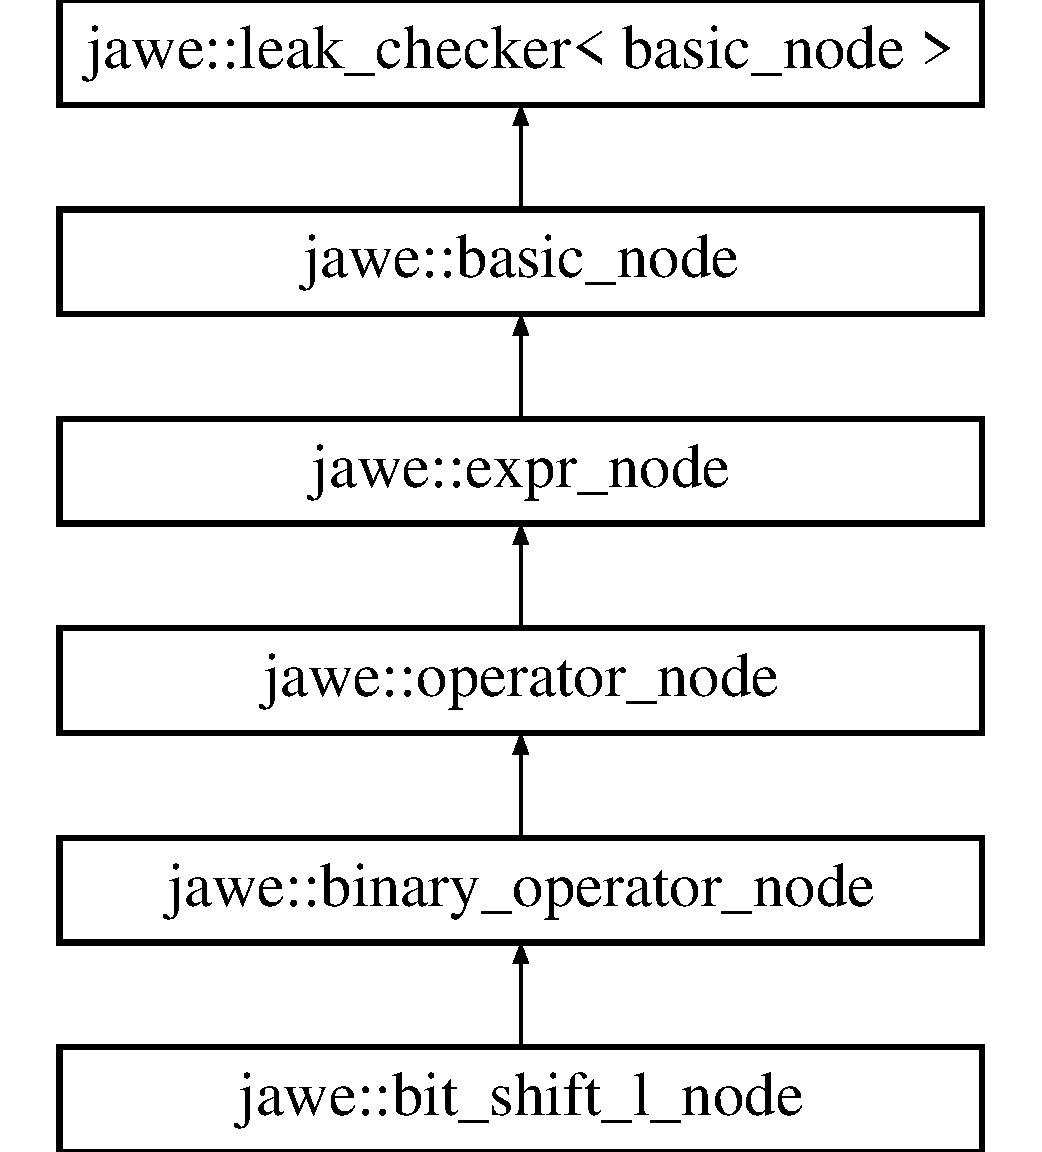
\includegraphics[height=6.000000cm]{classjawe_1_1bit__shift__l__node}
\end{center}
\end{figure}
\subsection*{Public Member Functions}
\begin{DoxyCompactItemize}
\item 
\hyperlink{classjawe_1_1bit__shift__l__node_aceb090920d486ee66b9dce574e72075c}{bit\+\_\+shift\+\_\+l\+\_\+node} (const \hyperlink{namespacejawe_a3f307481d921b6cbb50cc8511fc2b544}{shared\+\_\+node} \&, const \hyperlink{namespacejawe_a3f307481d921b6cbb50cc8511fc2b544}{shared\+\_\+node} \&)
\end{DoxyCompactItemize}
\subsection*{Additional Inherited Members}


\subsection{Constructor \& Destructor Documentation}
\mbox{\Hypertarget{classjawe_1_1bit__shift__l__node_aceb090920d486ee66b9dce574e72075c}\label{classjawe_1_1bit__shift__l__node_aceb090920d486ee66b9dce574e72075c}} 
\index{jawe\+::bit\+\_\+shift\+\_\+l\+\_\+node@{jawe\+::bit\+\_\+shift\+\_\+l\+\_\+node}!bit\+\_\+shift\+\_\+l\+\_\+node@{bit\+\_\+shift\+\_\+l\+\_\+node}}
\index{bit\+\_\+shift\+\_\+l\+\_\+node@{bit\+\_\+shift\+\_\+l\+\_\+node}!jawe\+::bit\+\_\+shift\+\_\+l\+\_\+node@{jawe\+::bit\+\_\+shift\+\_\+l\+\_\+node}}
\subsubsection{\texorpdfstring{bit\+\_\+shift\+\_\+l\+\_\+node()}{bit\_shift\_l\_node()}}
{\footnotesize\ttfamily bit\+\_\+shift\+\_\+l\+\_\+node\+::bit\+\_\+shift\+\_\+l\+\_\+node (\begin{DoxyParamCaption}\item[{const \hyperlink{namespacejawe_a3f307481d921b6cbb50cc8511fc2b544}{shared\+\_\+node} \&}]{left,  }\item[{const \hyperlink{namespacejawe_a3f307481d921b6cbb50cc8511fc2b544}{shared\+\_\+node} \&}]{right }\end{DoxyParamCaption})}



The documentation for this class was generated from the following files\+:\begin{DoxyCompactItemize}
\item 
include/syntax/operators/\hyperlink{bit__shift__l__node_8hpp}{bit\+\_\+shift\+\_\+l\+\_\+node.\+hpp}\item 
src/syntax/operators/\hyperlink{bit__shift__l__node_8cpp}{bit\+\_\+shift\+\_\+l\+\_\+node.\+cpp}\end{DoxyCompactItemize}

\hypertarget{classjawe_1_1bit__shift__r__node}{}\section{jawe\+:\+:bit\+\_\+shift\+\_\+r\+\_\+node Class Reference}
\label{classjawe_1_1bit__shift__r__node}\index{jawe\+::bit\+\_\+shift\+\_\+r\+\_\+node@{jawe\+::bit\+\_\+shift\+\_\+r\+\_\+node}}


{\ttfamily \#include $<$bit\+\_\+shift\+\_\+r\+\_\+node.\+hpp$>$}

Inheritance diagram for jawe\+:\+:bit\+\_\+shift\+\_\+r\+\_\+node\+:\begin{figure}[H]
\begin{center}
\leavevmode
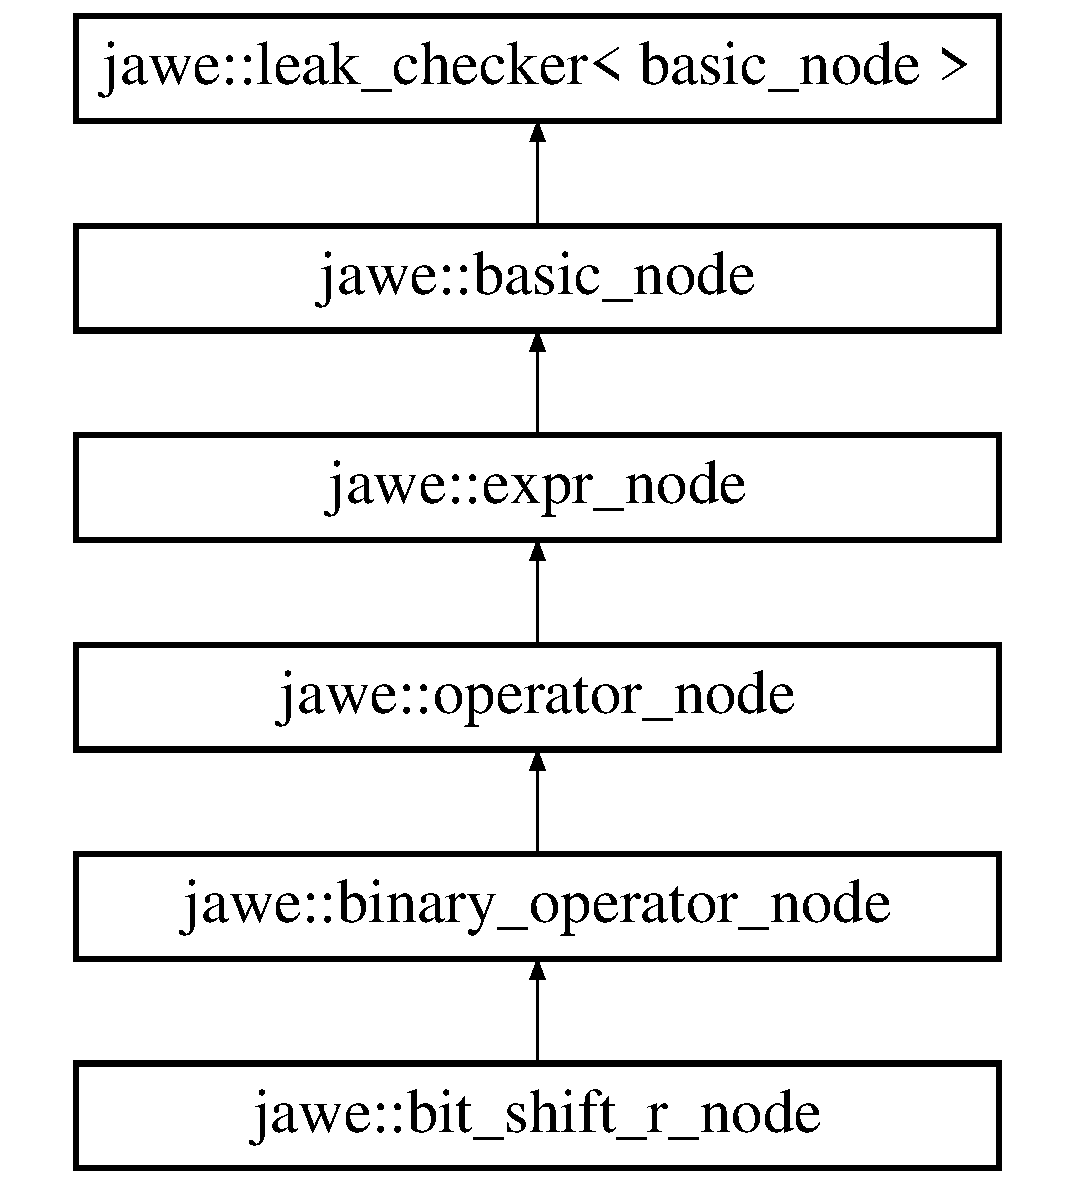
\includegraphics[height=6.000000cm]{classjawe_1_1bit__shift__r__node}
\end{center}
\end{figure}
\subsection*{Public Member Functions}
\begin{DoxyCompactItemize}
\item 
\hyperlink{classjawe_1_1bit__shift__r__node_a68feccd9fc1c2d51ee325ccd65603a98}{bit\+\_\+shift\+\_\+r\+\_\+node} (const \hyperlink{namespacejawe_a3f307481d921b6cbb50cc8511fc2b544}{shared\+\_\+node} \&, const \hyperlink{namespacejawe_a3f307481d921b6cbb50cc8511fc2b544}{shared\+\_\+node} \&)
\end{DoxyCompactItemize}
\subsection*{Additional Inherited Members}


\subsection{Constructor \& Destructor Documentation}
\mbox{\Hypertarget{classjawe_1_1bit__shift__r__node_a68feccd9fc1c2d51ee325ccd65603a98}\label{classjawe_1_1bit__shift__r__node_a68feccd9fc1c2d51ee325ccd65603a98}} 
\index{jawe\+::bit\+\_\+shift\+\_\+r\+\_\+node@{jawe\+::bit\+\_\+shift\+\_\+r\+\_\+node}!bit\+\_\+shift\+\_\+r\+\_\+node@{bit\+\_\+shift\+\_\+r\+\_\+node}}
\index{bit\+\_\+shift\+\_\+r\+\_\+node@{bit\+\_\+shift\+\_\+r\+\_\+node}!jawe\+::bit\+\_\+shift\+\_\+r\+\_\+node@{jawe\+::bit\+\_\+shift\+\_\+r\+\_\+node}}
\subsubsection{\texorpdfstring{bit\+\_\+shift\+\_\+r\+\_\+node()}{bit\_shift\_r\_node()}}
{\footnotesize\ttfamily bit\+\_\+shift\+\_\+r\+\_\+node\+::bit\+\_\+shift\+\_\+r\+\_\+node (\begin{DoxyParamCaption}\item[{const \hyperlink{namespacejawe_a3f307481d921b6cbb50cc8511fc2b544}{shared\+\_\+node} \&}]{left,  }\item[{const \hyperlink{namespacejawe_a3f307481d921b6cbb50cc8511fc2b544}{shared\+\_\+node} \&}]{right }\end{DoxyParamCaption})}



The documentation for this class was generated from the following files\+:\begin{DoxyCompactItemize}
\item 
include/syntax/operators/\hyperlink{bit__shift__r__node_8hpp}{bit\+\_\+shift\+\_\+r\+\_\+node.\+hpp}\item 
src/syntax/operators/\hyperlink{bit__shift__r__node_8cpp}{bit\+\_\+shift\+\_\+r\+\_\+node.\+cpp}\end{DoxyCompactItemize}

\hypertarget{classjawe_1_1bit__shift__u__node}{}\section{jawe\+:\+:bit\+\_\+shift\+\_\+u\+\_\+node Class Reference}
\label{classjawe_1_1bit__shift__u__node}\index{jawe\+::bit\+\_\+shift\+\_\+u\+\_\+node@{jawe\+::bit\+\_\+shift\+\_\+u\+\_\+node}}


{\ttfamily \#include $<$bit\+\_\+shift\+\_\+u\+\_\+node.\+hpp$>$}

Inheritance diagram for jawe\+:\+:bit\+\_\+shift\+\_\+u\+\_\+node\+:\begin{figure}[H]
\begin{center}
\leavevmode
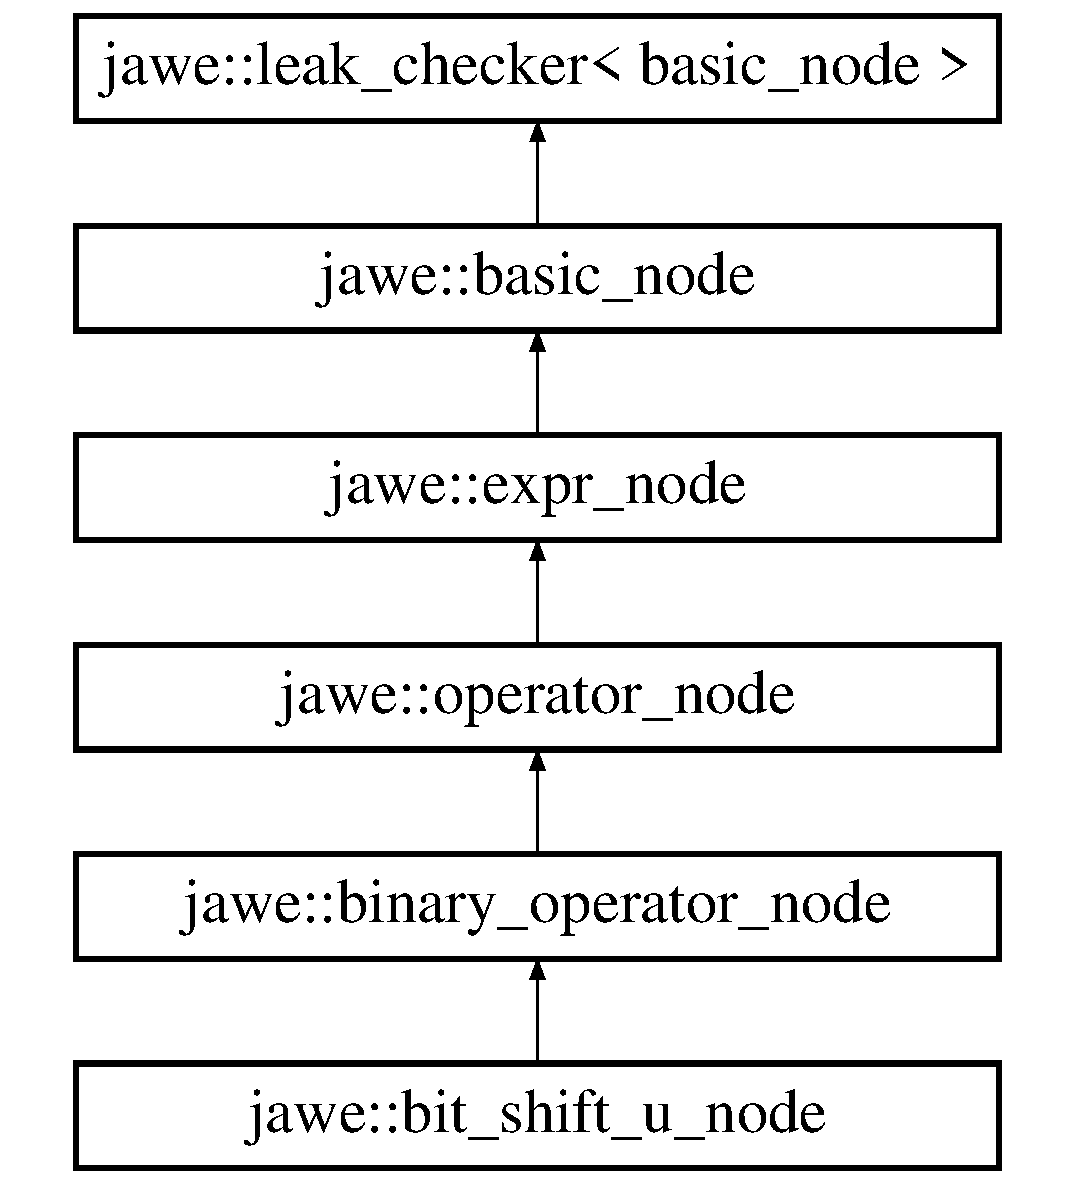
\includegraphics[height=6.000000cm]{classjawe_1_1bit__shift__u__node}
\end{center}
\end{figure}
\subsection*{Public Member Functions}
\begin{DoxyCompactItemize}
\item 
\hyperlink{classjawe_1_1bit__shift__u__node_a786ec5035cd91619636126a2bcc01c54}{bit\+\_\+shift\+\_\+u\+\_\+node} (const \hyperlink{namespacejawe_a3f307481d921b6cbb50cc8511fc2b544}{shared\+\_\+node} \&, const \hyperlink{namespacejawe_a3f307481d921b6cbb50cc8511fc2b544}{shared\+\_\+node} \&)
\end{DoxyCompactItemize}
\subsection*{Additional Inherited Members}


\subsection{Constructor \& Destructor Documentation}
\mbox{\Hypertarget{classjawe_1_1bit__shift__u__node_a786ec5035cd91619636126a2bcc01c54}\label{classjawe_1_1bit__shift__u__node_a786ec5035cd91619636126a2bcc01c54}} 
\index{jawe\+::bit\+\_\+shift\+\_\+u\+\_\+node@{jawe\+::bit\+\_\+shift\+\_\+u\+\_\+node}!bit\+\_\+shift\+\_\+u\+\_\+node@{bit\+\_\+shift\+\_\+u\+\_\+node}}
\index{bit\+\_\+shift\+\_\+u\+\_\+node@{bit\+\_\+shift\+\_\+u\+\_\+node}!jawe\+::bit\+\_\+shift\+\_\+u\+\_\+node@{jawe\+::bit\+\_\+shift\+\_\+u\+\_\+node}}
\subsubsection{\texorpdfstring{bit\+\_\+shift\+\_\+u\+\_\+node()}{bit\_shift\_u\_node()}}
{\footnotesize\ttfamily bit\+\_\+shift\+\_\+u\+\_\+node\+::bit\+\_\+shift\+\_\+u\+\_\+node (\begin{DoxyParamCaption}\item[{const \hyperlink{namespacejawe_a3f307481d921b6cbb50cc8511fc2b544}{shared\+\_\+node} \&}]{left,  }\item[{const \hyperlink{namespacejawe_a3f307481d921b6cbb50cc8511fc2b544}{shared\+\_\+node} \&}]{right }\end{DoxyParamCaption})}



The documentation for this class was generated from the following files\+:\begin{DoxyCompactItemize}
\item 
include/syntax/operators/\hyperlink{bit__shift__u__node_8hpp}{bit\+\_\+shift\+\_\+u\+\_\+node.\+hpp}\item 
src/syntax/operators/\hyperlink{bit__shift__u__node_8cpp}{bit\+\_\+shift\+\_\+u\+\_\+node.\+cpp}\end{DoxyCompactItemize}

\hypertarget{classjawe_1_1bit__xor__node}{}\section{jawe\+:\+:bit\+\_\+xor\+\_\+node Class Reference}
\label{classjawe_1_1bit__xor__node}\index{jawe\+::bit\+\_\+xor\+\_\+node@{jawe\+::bit\+\_\+xor\+\_\+node}}


{\ttfamily \#include $<$bit\+\_\+xor\+\_\+node.\+hpp$>$}

Inheritance diagram for jawe\+:\+:bit\+\_\+xor\+\_\+node\+:\begin{figure}[H]
\begin{center}
\leavevmode
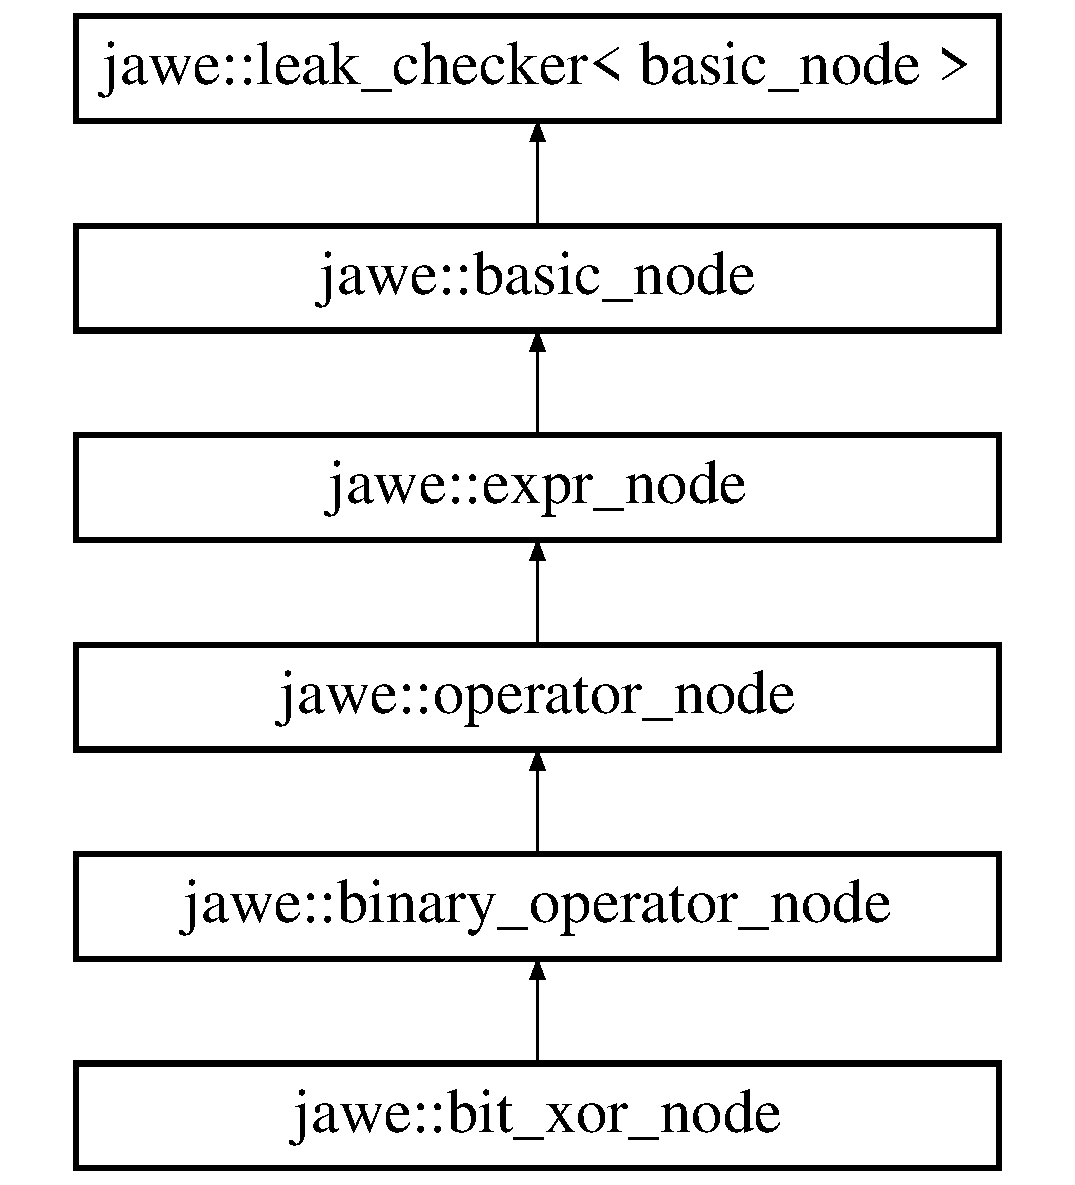
\includegraphics[height=6.000000cm]{classjawe_1_1bit__xor__node}
\end{center}
\end{figure}
\subsection*{Public Member Functions}
\begin{DoxyCompactItemize}
\item 
\hyperlink{classjawe_1_1bit__xor__node_a0c2e60807baf846ba1bba6c1a0564d48}{bit\+\_\+xor\+\_\+node} (const \hyperlink{namespacejawe_a3f307481d921b6cbb50cc8511fc2b544}{shared\+\_\+node} \&, const \hyperlink{namespacejawe_a3f307481d921b6cbb50cc8511fc2b544}{shared\+\_\+node} \&)
\end{DoxyCompactItemize}
\subsection*{Additional Inherited Members}


\subsection{Constructor \& Destructor Documentation}
\mbox{\Hypertarget{classjawe_1_1bit__xor__node_a0c2e60807baf846ba1bba6c1a0564d48}\label{classjawe_1_1bit__xor__node_a0c2e60807baf846ba1bba6c1a0564d48}} 
\index{jawe\+::bit\+\_\+xor\+\_\+node@{jawe\+::bit\+\_\+xor\+\_\+node}!bit\+\_\+xor\+\_\+node@{bit\+\_\+xor\+\_\+node}}
\index{bit\+\_\+xor\+\_\+node@{bit\+\_\+xor\+\_\+node}!jawe\+::bit\+\_\+xor\+\_\+node@{jawe\+::bit\+\_\+xor\+\_\+node}}
\subsubsection{\texorpdfstring{bit\+\_\+xor\+\_\+node()}{bit\_xor\_node()}}
{\footnotesize\ttfamily bit\+\_\+xor\+\_\+node\+::bit\+\_\+xor\+\_\+node (\begin{DoxyParamCaption}\item[{const \hyperlink{namespacejawe_a3f307481d921b6cbb50cc8511fc2b544}{shared\+\_\+node} \&}]{left,  }\item[{const \hyperlink{namespacejawe_a3f307481d921b6cbb50cc8511fc2b544}{shared\+\_\+node} \&}]{right }\end{DoxyParamCaption})}



The documentation for this class was generated from the following files\+:\begin{DoxyCompactItemize}
\item 
include/syntax/operators/\hyperlink{bit__xor__node_8hpp}{bit\+\_\+xor\+\_\+node.\+hpp}\item 
src/syntax/operators/\hyperlink{bit__xor__node_8cpp}{bit\+\_\+xor\+\_\+node.\+cpp}\end{DoxyCompactItemize}

\hypertarget{classjawe_1_1break__node}{}\section{jawe\+:\+:break\+\_\+node Class Reference}
\label{classjawe_1_1break__node}\index{jawe\+::break\+\_\+node@{jawe\+::break\+\_\+node}}


{\ttfamily \#include $<$break\+\_\+node.\+hpp$>$}

Inheritance diagram for jawe\+:\+:break\+\_\+node\+:\begin{figure}[H]
\begin{center}
\leavevmode
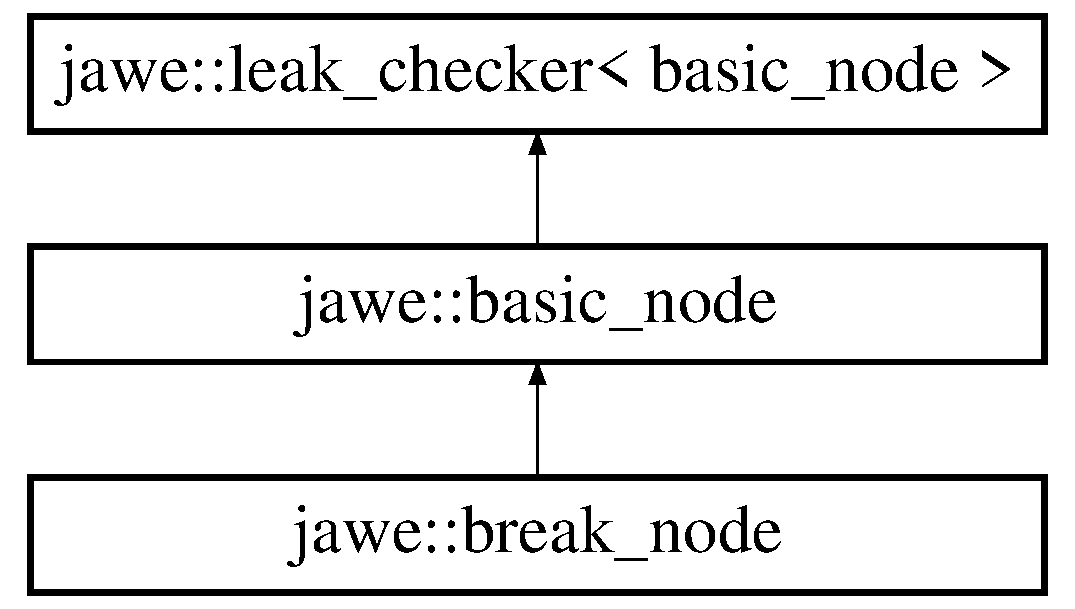
\includegraphics[height=3.000000cm]{classjawe_1_1break__node}
\end{center}
\end{figure}
\subsection*{Public Member Functions}
\begin{DoxyCompactItemize}
\item 
\hyperlink{classjawe_1_1break__node_a7993d43d6ec51f1895c2a7351b931a5e}{break\+\_\+node} ()
\end{DoxyCompactItemize}
\subsection*{Additional Inherited Members}


\subsection{Constructor \& Destructor Documentation}
\mbox{\Hypertarget{classjawe_1_1break__node_a7993d43d6ec51f1895c2a7351b931a5e}\label{classjawe_1_1break__node_a7993d43d6ec51f1895c2a7351b931a5e}} 
\index{jawe\+::break\+\_\+node@{jawe\+::break\+\_\+node}!break\+\_\+node@{break\+\_\+node}}
\index{break\+\_\+node@{break\+\_\+node}!jawe\+::break\+\_\+node@{jawe\+::break\+\_\+node}}
\subsubsection{\texorpdfstring{break\+\_\+node()}{break\_node()}}
{\footnotesize\ttfamily break\+\_\+node\+::break\+\_\+node (\begin{DoxyParamCaption}{ }\end{DoxyParamCaption})}



The documentation for this class was generated from the following files\+:\begin{DoxyCompactItemize}
\item 
include/syntax/control\+\_\+flow/\hyperlink{break__node_8hpp}{break\+\_\+node.\+hpp}\item 
src/syntax/control\+\_\+flow/\hyperlink{break__node_8cpp}{break\+\_\+node.\+cpp}\end{DoxyCompactItemize}

\hypertarget{classjawe_1_1case__node}{}\section{jawe\+:\+:case\+\_\+node Class Reference}
\label{classjawe_1_1case__node}\index{jawe\+::case\+\_\+node@{jawe\+::case\+\_\+node}}


{\ttfamily \#include $<$case\+\_\+node.\+hpp$>$}

Inheritance diagram for jawe\+:\+:case\+\_\+node\+:\begin{figure}[H]
\begin{center}
\leavevmode
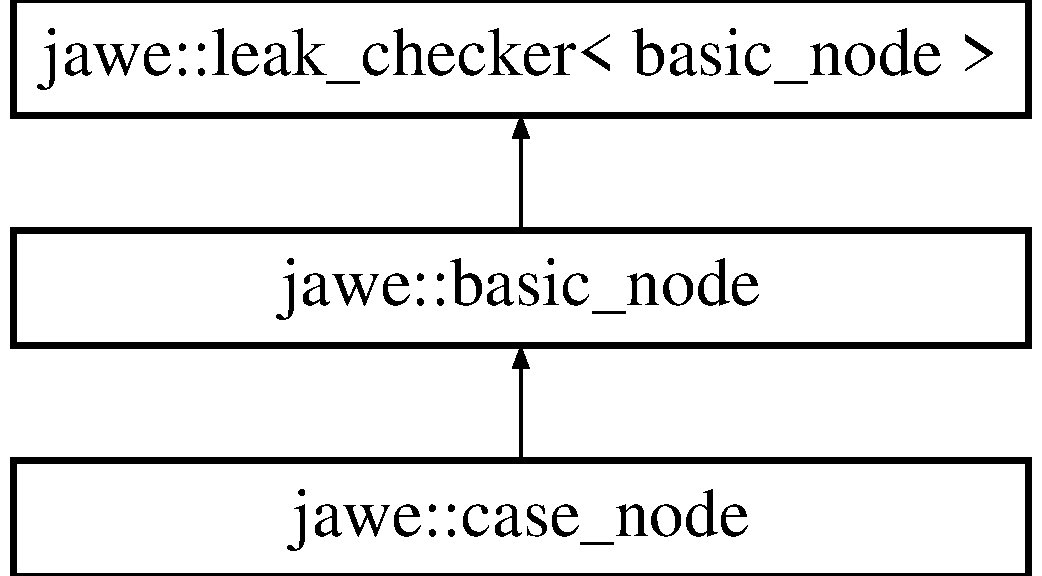
\includegraphics[height=3.000000cm]{classjawe_1_1case__node}
\end{center}
\end{figure}
\subsection*{Public Member Functions}
\begin{DoxyCompactItemize}
\item 
\hyperlink{classjawe_1_1case__node_a99b22c0a8ef6b596439a876510ee790a}{case\+\_\+node} (const \hyperlink{namespacejawe_a3f307481d921b6cbb50cc8511fc2b544}{shared\+\_\+node} \&, const \hyperlink{namespacejawe_a3f307481d921b6cbb50cc8511fc2b544}{shared\+\_\+node} \&)
\item 
\hyperlink{namespacejawe_a3f307481d921b6cbb50cc8511fc2b544}{shared\+\_\+node} \hyperlink{classjawe_1_1case__node_a04a49f28923cf8ea3faee431bd6797e7}{get\+\_\+body} () const
\item 
\hyperlink{namespacejawe_a3f307481d921b6cbb50cc8511fc2b544}{shared\+\_\+node} \hyperlink{classjawe_1_1case__node_a005b7e103d6dec24adf567f7be67d363}{get\+\_\+case} () const
\end{DoxyCompactItemize}
\subsection*{Private Attributes}
\begin{DoxyCompactItemize}
\item 
\hyperlink{namespacejawe_a3f307481d921b6cbb50cc8511fc2b544}{shared\+\_\+node} \hyperlink{classjawe_1_1case__node_a8d02757ea9e3677d4ff6be8fc01112b6}{m\+\_\+case}
\item 
\hyperlink{namespacejawe_a3f307481d921b6cbb50cc8511fc2b544}{shared\+\_\+node} \hyperlink{classjawe_1_1case__node_a50358640675afacd6a8a11d9c4edbb23}{m\+\_\+body}
\end{DoxyCompactItemize}
\subsection*{Additional Inherited Members}


\subsection{Constructor \& Destructor Documentation}
\mbox{\Hypertarget{classjawe_1_1case__node_a99b22c0a8ef6b596439a876510ee790a}\label{classjawe_1_1case__node_a99b22c0a8ef6b596439a876510ee790a}} 
\index{jawe\+::case\+\_\+node@{jawe\+::case\+\_\+node}!case\+\_\+node@{case\+\_\+node}}
\index{case\+\_\+node@{case\+\_\+node}!jawe\+::case\+\_\+node@{jawe\+::case\+\_\+node}}
\subsubsection{\texorpdfstring{case\+\_\+node()}{case\_node()}}
{\footnotesize\ttfamily case\+\_\+node\+::case\+\_\+node (\begin{DoxyParamCaption}\item[{const \hyperlink{namespacejawe_a3f307481d921b6cbb50cc8511fc2b544}{shared\+\_\+node} \&}]{p,  }\item[{const \hyperlink{namespacejawe_a3f307481d921b6cbb50cc8511fc2b544}{shared\+\_\+node} \&}]{command }\end{DoxyParamCaption})}



\subsection{Member Function Documentation}
\mbox{\Hypertarget{classjawe_1_1case__node_a04a49f28923cf8ea3faee431bd6797e7}\label{classjawe_1_1case__node_a04a49f28923cf8ea3faee431bd6797e7}} 
\index{jawe\+::case\+\_\+node@{jawe\+::case\+\_\+node}!get\+\_\+body@{get\+\_\+body}}
\index{get\+\_\+body@{get\+\_\+body}!jawe\+::case\+\_\+node@{jawe\+::case\+\_\+node}}
\subsubsection{\texorpdfstring{get\+\_\+body()}{get\_body()}}
{\footnotesize\ttfamily \hyperlink{namespacejawe_a3f307481d921b6cbb50cc8511fc2b544}{shared\+\_\+node} case\+\_\+node\+::get\+\_\+body (\begin{DoxyParamCaption}{ }\end{DoxyParamCaption}) const}

\mbox{\Hypertarget{classjawe_1_1case__node_a005b7e103d6dec24adf567f7be67d363}\label{classjawe_1_1case__node_a005b7e103d6dec24adf567f7be67d363}} 
\index{jawe\+::case\+\_\+node@{jawe\+::case\+\_\+node}!get\+\_\+case@{get\+\_\+case}}
\index{get\+\_\+case@{get\+\_\+case}!jawe\+::case\+\_\+node@{jawe\+::case\+\_\+node}}
\subsubsection{\texorpdfstring{get\+\_\+case()}{get\_case()}}
{\footnotesize\ttfamily \hyperlink{namespacejawe_a3f307481d921b6cbb50cc8511fc2b544}{shared\+\_\+node} case\+\_\+node\+::get\+\_\+case (\begin{DoxyParamCaption}{ }\end{DoxyParamCaption}) const}



\subsection{Member Data Documentation}
\mbox{\Hypertarget{classjawe_1_1case__node_a50358640675afacd6a8a11d9c4edbb23}\label{classjawe_1_1case__node_a50358640675afacd6a8a11d9c4edbb23}} 
\index{jawe\+::case\+\_\+node@{jawe\+::case\+\_\+node}!m\+\_\+body@{m\+\_\+body}}
\index{m\+\_\+body@{m\+\_\+body}!jawe\+::case\+\_\+node@{jawe\+::case\+\_\+node}}
\subsubsection{\texorpdfstring{m\+\_\+body}{m\_body}}
{\footnotesize\ttfamily \hyperlink{namespacejawe_a3f307481d921b6cbb50cc8511fc2b544}{shared\+\_\+node} jawe\+::case\+\_\+node\+::m\+\_\+body\hspace{0.3cm}{\ttfamily [private]}}

\mbox{\Hypertarget{classjawe_1_1case__node_a8d02757ea9e3677d4ff6be8fc01112b6}\label{classjawe_1_1case__node_a8d02757ea9e3677d4ff6be8fc01112b6}} 
\index{jawe\+::case\+\_\+node@{jawe\+::case\+\_\+node}!m\+\_\+case@{m\+\_\+case}}
\index{m\+\_\+case@{m\+\_\+case}!jawe\+::case\+\_\+node@{jawe\+::case\+\_\+node}}
\subsubsection{\texorpdfstring{m\+\_\+case}{m\_case}}
{\footnotesize\ttfamily \hyperlink{namespacejawe_a3f307481d921b6cbb50cc8511fc2b544}{shared\+\_\+node} jawe\+::case\+\_\+node\+::m\+\_\+case\hspace{0.3cm}{\ttfamily [private]}}



The documentation for this class was generated from the following files\+:\begin{DoxyCompactItemize}
\item 
include/syntax/control\+\_\+flow/\hyperlink{case__node_8hpp}{case\+\_\+node.\+hpp}\item 
src/syntax/control\+\_\+flow/\hyperlink{case__node_8cpp}{case\+\_\+node.\+cpp}\end{DoxyCompactItemize}

\hypertarget{classjawe_1_1code__generator}{}\section{jawe\+:\+:code\+\_\+generator Class Reference}
\label{classjawe_1_1code__generator}\index{jawe\+::code\+\_\+generator@{jawe\+::code\+\_\+generator}}


{\ttfamily \#include $<$code\+\_\+generator.\+hpp$>$}

Inheritance diagram for jawe\+:\+:code\+\_\+generator\+:\begin{figure}[H]
\begin{center}
\leavevmode
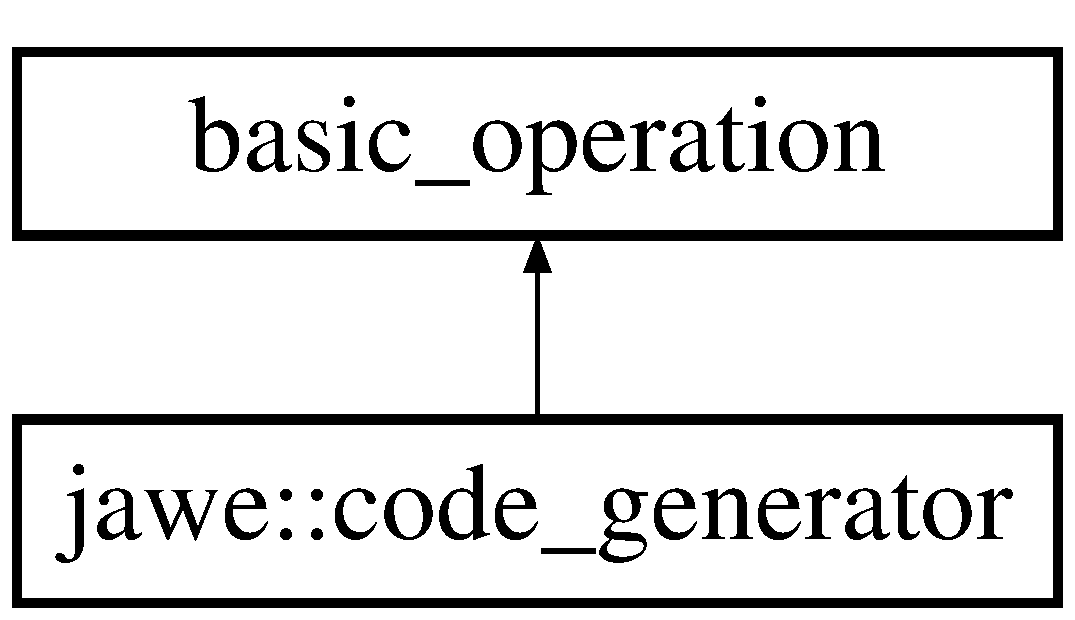
\includegraphics[height=2.000000cm]{classjawe_1_1code__generator}
\end{center}
\end{figure}
\subsection*{Public Member Functions}
\begin{DoxyCompactItemize}
\item 
\hyperlink{classjawe_1_1code__generator_a1218452973234e90972be154fc25bf92}{code\+\_\+generator} ()
\item 
void \hyperlink{classjawe_1_1code__generator_af280f3dcaeb6cbbf30b5e9eb55771b21}{run} ()
\end{DoxyCompactItemize}
\subsection*{Private Member Functions}
\begin{DoxyCompactItemize}
\item 
llvm\+::\+Value $\ast$ \hyperlink{classjawe_1_1code__generator_a88b1f6fff308ef1b6c3b63d211a457f3}{codegen} (const \hyperlink{namespacejawe_a3f307481d921b6cbb50cc8511fc2b544}{shared\+\_\+node} \&)
\item 
llvm\+::\+Alloca\+Inst $\ast$ \hyperlink{classjawe_1_1code__generator_a508a01a4a5d0c53070d3186640ccb8c5}{create\+\_\+alloca} (llvm\+::\+Function $\ast$, const char $\ast$) const
\end{DoxyCompactItemize}
\subsection*{Private Attributes}
\begin{DoxyCompactItemize}
\item 
llvm\+::\+I\+R\+Builder \hyperlink{classjawe_1_1code__generator_aad2f012dfc4d811c02e4e580d4fd3390}{m\+\_\+ir\+\_\+builder}
\item 
\hyperlink{classjawe_1_1utils_1_1scope}{utils\+::scope}$<$ llvm\+::\+Alloca\+Inst $\ast$ $>$ \hyperlink{classjawe_1_1code__generator_a209dd65e5b96fd20ea63fdb13f17b052}{m\+\_\+scopes}
\end{DoxyCompactItemize}


\subsection{Constructor \& Destructor Documentation}
\mbox{\Hypertarget{classjawe_1_1code__generator_a1218452973234e90972be154fc25bf92}\label{classjawe_1_1code__generator_a1218452973234e90972be154fc25bf92}} 
\index{jawe\+::code\+\_\+generator@{jawe\+::code\+\_\+generator}!code\+\_\+generator@{code\+\_\+generator}}
\index{code\+\_\+generator@{code\+\_\+generator}!jawe\+::code\+\_\+generator@{jawe\+::code\+\_\+generator}}
\subsubsection{\texorpdfstring{code\+\_\+generator()}{code\_generator()}}
{\footnotesize\ttfamily code\+\_\+generator\+::code\+\_\+generator (\begin{DoxyParamCaption}{ }\end{DoxyParamCaption})}



\subsection{Member Function Documentation}
\mbox{\Hypertarget{classjawe_1_1code__generator_a88b1f6fff308ef1b6c3b63d211a457f3}\label{classjawe_1_1code__generator_a88b1f6fff308ef1b6c3b63d211a457f3}} 
\index{jawe\+::code\+\_\+generator@{jawe\+::code\+\_\+generator}!codegen@{codegen}}
\index{codegen@{codegen}!jawe\+::code\+\_\+generator@{jawe\+::code\+\_\+generator}}
\subsubsection{\texorpdfstring{codegen()}{codegen()}}
{\footnotesize\ttfamily llvm\+::\+Value $\ast$ code\+\_\+generator\+::codegen (\begin{DoxyParamCaption}\item[{const \hyperlink{namespacejawe_a3f307481d921b6cbb50cc8511fc2b544}{shared\+\_\+node} \&}]{root }\end{DoxyParamCaption})\hspace{0.3cm}{\ttfamily [private]}}

\mbox{\Hypertarget{classjawe_1_1code__generator_a508a01a4a5d0c53070d3186640ccb8c5}\label{classjawe_1_1code__generator_a508a01a4a5d0c53070d3186640ccb8c5}} 
\index{jawe\+::code\+\_\+generator@{jawe\+::code\+\_\+generator}!create\+\_\+alloca@{create\+\_\+alloca}}
\index{create\+\_\+alloca@{create\+\_\+alloca}!jawe\+::code\+\_\+generator@{jawe\+::code\+\_\+generator}}
\subsubsection{\texorpdfstring{create\+\_\+alloca()}{create\_alloca()}}
{\footnotesize\ttfamily llvm\+::\+Alloca\+Inst $\ast$ code\+\_\+generator\+::create\+\_\+alloca (\begin{DoxyParamCaption}\item[{llvm\+::\+Function $\ast$}]{f,  }\item[{const char $\ast$}]{var\+\_\+name }\end{DoxyParamCaption}) const\hspace{0.3cm}{\ttfamily [private]}}

\mbox{\Hypertarget{classjawe_1_1code__generator_af280f3dcaeb6cbbf30b5e9eb55771b21}\label{classjawe_1_1code__generator_af280f3dcaeb6cbbf30b5e9eb55771b21}} 
\index{jawe\+::code\+\_\+generator@{jawe\+::code\+\_\+generator}!run@{run}}
\index{run@{run}!jawe\+::code\+\_\+generator@{jawe\+::code\+\_\+generator}}
\subsubsection{\texorpdfstring{run()}{run()}}
{\footnotesize\ttfamily void code\+\_\+generator\+::run (\begin{DoxyParamCaption}{ }\end{DoxyParamCaption})}



\subsection{Member Data Documentation}
\mbox{\Hypertarget{classjawe_1_1code__generator_aad2f012dfc4d811c02e4e580d4fd3390}\label{classjawe_1_1code__generator_aad2f012dfc4d811c02e4e580d4fd3390}} 
\index{jawe\+::code\+\_\+generator@{jawe\+::code\+\_\+generator}!m\+\_\+ir\+\_\+builder@{m\+\_\+ir\+\_\+builder}}
\index{m\+\_\+ir\+\_\+builder@{m\+\_\+ir\+\_\+builder}!jawe\+::code\+\_\+generator@{jawe\+::code\+\_\+generator}}
\subsubsection{\texorpdfstring{m\+\_\+ir\+\_\+builder}{m\_ir\_builder}}
{\footnotesize\ttfamily llvm\+::\+I\+R\+Builder jawe\+::code\+\_\+generator\+::m\+\_\+ir\+\_\+builder\hspace{0.3cm}{\ttfamily [private]}}

\mbox{\Hypertarget{classjawe_1_1code__generator_a209dd65e5b96fd20ea63fdb13f17b052}\label{classjawe_1_1code__generator_a209dd65e5b96fd20ea63fdb13f17b052}} 
\index{jawe\+::code\+\_\+generator@{jawe\+::code\+\_\+generator}!m\+\_\+scopes@{m\+\_\+scopes}}
\index{m\+\_\+scopes@{m\+\_\+scopes}!jawe\+::code\+\_\+generator@{jawe\+::code\+\_\+generator}}
\subsubsection{\texorpdfstring{m\+\_\+scopes}{m\_scopes}}
{\footnotesize\ttfamily \hyperlink{classjawe_1_1utils_1_1scope}{utils\+::scope}$<$llvm\+::\+Alloca\+Inst$\ast$$>$ jawe\+::code\+\_\+generator\+::m\+\_\+scopes\hspace{0.3cm}{\ttfamily [private]}}



The documentation for this class was generated from the following files\+:\begin{DoxyCompactItemize}
\item 
include/operations/\hyperlink{code__generator_8hpp}{code\+\_\+generator.\+hpp}\item 
src/operations/\hyperlink{code__generator_8cpp}{code\+\_\+generator.\+cpp}\end{DoxyCompactItemize}

\hypertarget{classjawe_1_1command__block__node}{}\section{jawe\+:\+:command\+\_\+block\+\_\+node Class Reference}
\label{classjawe_1_1command__block__node}\index{jawe\+::command\+\_\+block\+\_\+node@{jawe\+::command\+\_\+block\+\_\+node}}


{\ttfamily \#include $<$command\+\_\+block\+\_\+node.\+hpp$>$}

Inheritance diagram for jawe\+:\+:command\+\_\+block\+\_\+node\+:\begin{figure}[H]
\begin{center}
\leavevmode
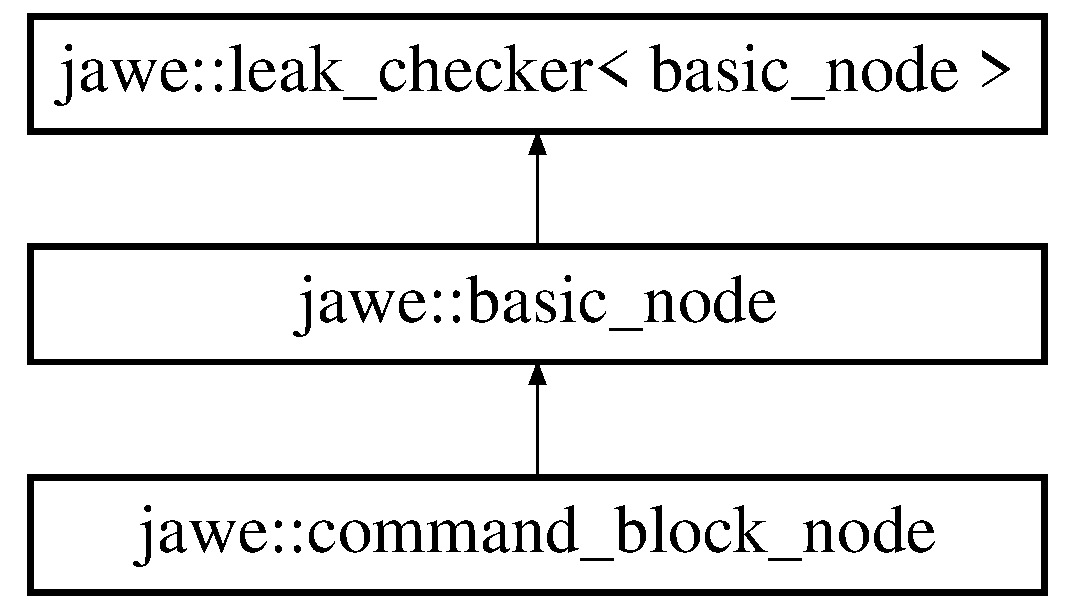
\includegraphics[height=3.000000cm]{classjawe_1_1command__block__node}
\end{center}
\end{figure}
\subsection*{Public Member Functions}
\begin{DoxyCompactItemize}
\item 
\hyperlink{classjawe_1_1command__block__node_a3114c27da8e02aaecae198adbc2444b7}{command\+\_\+block\+\_\+node} ()
\item 
\hyperlink{classjawe_1_1command__block__node_a833c98a4433d6ccffe9eca004cc92fdd}{command\+\_\+block\+\_\+node} (const \hyperlink{namespacejawe_a3f307481d921b6cbb50cc8511fc2b544}{shared\+\_\+node} \&)
\item 
\hyperlink{classjawe_1_1command__block__node_a4cbb669292fd23c022260f0b5ca6e88d}{command\+\_\+block\+\_\+node} (const std\+::vector$<$ \hyperlink{namespacejawe_a3f307481d921b6cbb50cc8511fc2b544}{shared\+\_\+node} $>$ \&)
\item 
void \hyperlink{classjawe_1_1command__block__node_acd62202eefef834ec691c91aef0692a5}{push\+\_\+back} (const \hyperlink{namespacejawe_a3f307481d921b6cbb50cc8511fc2b544}{shared\+\_\+node} \&)
\item 
void \hyperlink{classjawe_1_1command__block__node_a2e8b9839521f0b6020dc07ed12bfd952}{push\+\_\+back\+\_\+fun\+\_\+decl} (const \hyperlink{namespacejawe_a3f307481d921b6cbb50cc8511fc2b544}{shared\+\_\+node} \&)
\item 
void \hyperlink{classjawe_1_1command__block__node_a6b9109910ce8f64c7713f2d0bcf0407a}{push\+\_\+back\+\_\+var\+\_\+decl} (const \hyperlink{namespacejawe_a3f307481d921b6cbb50cc8511fc2b544}{shared\+\_\+node} \&)
\item 
std\+::vector$<$ \hyperlink{namespacejawe_a3f307481d921b6cbb50cc8511fc2b544}{shared\+\_\+node} $>$ \hyperlink{classjawe_1_1command__block__node_ab3c22d98d1174a7f2a3fc35ed1fae74b}{get\+\_\+commands} ()
\item 
void \hyperlink{classjawe_1_1command__block__node_a0eece1d8e15227e437204a6316ed5feb}{remove} (const \hyperlink{namespacejawe_a3f307481d921b6cbb50cc8511fc2b544}{shared\+\_\+node} \&)
\item 
void \hyperlink{classjawe_1_1command__block__node_a8100afe1d2ba0df43c8ac7827ced9d31}{remove\+\_\+command} (const \hyperlink{namespacejawe_a3f307481d921b6cbb50cc8511fc2b544}{shared\+\_\+node} \&)
\item 
void \hyperlink{classjawe_1_1command__block__node_a092957384e4095db729dc4f032676e59}{remove\+\_\+fun\+\_\+decl} (const \hyperlink{namespacejawe_a3f307481d921b6cbb50cc8511fc2b544}{shared\+\_\+node} \&)
\item 
void \hyperlink{classjawe_1_1command__block__node_ae06b2258671be36bbd1401c53363e9b4}{remove\+\_\+var\+\_\+decl} (const \hyperlink{namespacejawe_a3f307481d921b6cbb50cc8511fc2b544}{shared\+\_\+node} \&)
\item 
void \hyperlink{classjawe_1_1command__block__node_a0a4f2c34d319286001d2ac7992d310df}{replace} (const \hyperlink{namespacejawe_a3f307481d921b6cbb50cc8511fc2b544}{shared\+\_\+node} \&, \hyperlink{namespacejawe_a3f307481d921b6cbb50cc8511fc2b544}{shared\+\_\+node} \&\&)
\end{DoxyCompactItemize}
\subsection*{Private Attributes}
\begin{DoxyCompactItemize}
\item 
std\+::vector$<$ \hyperlink{namespacejawe_a3f307481d921b6cbb50cc8511fc2b544}{shared\+\_\+node} $>$ \hyperlink{classjawe_1_1command__block__node_a1305c1454886bd3c1aa6a7ae293d1301}{m\+\_\+fun\+\_\+declarations}
\item 
std\+::vector$<$ \hyperlink{namespacejawe_a3f307481d921b6cbb50cc8511fc2b544}{shared\+\_\+node} $>$ \hyperlink{classjawe_1_1command__block__node_a20dbb8211a19cbbf46e85f61e31d4695}{m\+\_\+var\+\_\+declarations}
\item 
std\+::vector$<$ \hyperlink{namespacejawe_a3f307481d921b6cbb50cc8511fc2b544}{shared\+\_\+node} $>$ \hyperlink{classjawe_1_1command__block__node_a33e8d6b53bb74acb1364769a9f240dd5}{m\+\_\+commands}
\end{DoxyCompactItemize}
\subsection*{Additional Inherited Members}


\subsection{Constructor \& Destructor Documentation}
\mbox{\Hypertarget{classjawe_1_1command__block__node_a3114c27da8e02aaecae198adbc2444b7}\label{classjawe_1_1command__block__node_a3114c27da8e02aaecae198adbc2444b7}} 
\index{jawe\+::command\+\_\+block\+\_\+node@{jawe\+::command\+\_\+block\+\_\+node}!command\+\_\+block\+\_\+node@{command\+\_\+block\+\_\+node}}
\index{command\+\_\+block\+\_\+node@{command\+\_\+block\+\_\+node}!jawe\+::command\+\_\+block\+\_\+node@{jawe\+::command\+\_\+block\+\_\+node}}
\subsubsection{\texorpdfstring{command\+\_\+block\+\_\+node()}{command\_block\_node()}\hspace{0.1cm}{\footnotesize\ttfamily [1/3]}}
{\footnotesize\ttfamily command\+\_\+block\+\_\+node\+::command\+\_\+block\+\_\+node (\begin{DoxyParamCaption}{ }\end{DoxyParamCaption})}

\mbox{\Hypertarget{classjawe_1_1command__block__node_a833c98a4433d6ccffe9eca004cc92fdd}\label{classjawe_1_1command__block__node_a833c98a4433d6ccffe9eca004cc92fdd}} 
\index{jawe\+::command\+\_\+block\+\_\+node@{jawe\+::command\+\_\+block\+\_\+node}!command\+\_\+block\+\_\+node@{command\+\_\+block\+\_\+node}}
\index{command\+\_\+block\+\_\+node@{command\+\_\+block\+\_\+node}!jawe\+::command\+\_\+block\+\_\+node@{jawe\+::command\+\_\+block\+\_\+node}}
\subsubsection{\texorpdfstring{command\+\_\+block\+\_\+node()}{command\_block\_node()}\hspace{0.1cm}{\footnotesize\ttfamily [2/3]}}
{\footnotesize\ttfamily command\+\_\+block\+\_\+node\+::command\+\_\+block\+\_\+node (\begin{DoxyParamCaption}\item[{const \hyperlink{namespacejawe_a3f307481d921b6cbb50cc8511fc2b544}{shared\+\_\+node} \&}]{command }\end{DoxyParamCaption})}

\mbox{\Hypertarget{classjawe_1_1command__block__node_a4cbb669292fd23c022260f0b5ca6e88d}\label{classjawe_1_1command__block__node_a4cbb669292fd23c022260f0b5ca6e88d}} 
\index{jawe\+::command\+\_\+block\+\_\+node@{jawe\+::command\+\_\+block\+\_\+node}!command\+\_\+block\+\_\+node@{command\+\_\+block\+\_\+node}}
\index{command\+\_\+block\+\_\+node@{command\+\_\+block\+\_\+node}!jawe\+::command\+\_\+block\+\_\+node@{jawe\+::command\+\_\+block\+\_\+node}}
\subsubsection{\texorpdfstring{command\+\_\+block\+\_\+node()}{command\_block\_node()}\hspace{0.1cm}{\footnotesize\ttfamily [3/3]}}
{\footnotesize\ttfamily command\+\_\+block\+\_\+node\+::command\+\_\+block\+\_\+node (\begin{DoxyParamCaption}\item[{const std\+::vector$<$ \hyperlink{namespacejawe_a3f307481d921b6cbb50cc8511fc2b544}{shared\+\_\+node} $>$ \&}]{commands }\end{DoxyParamCaption})}



\subsection{Member Function Documentation}
\mbox{\Hypertarget{classjawe_1_1command__block__node_ab3c22d98d1174a7f2a3fc35ed1fae74b}\label{classjawe_1_1command__block__node_ab3c22d98d1174a7f2a3fc35ed1fae74b}} 
\index{jawe\+::command\+\_\+block\+\_\+node@{jawe\+::command\+\_\+block\+\_\+node}!get\+\_\+commands@{get\+\_\+commands}}
\index{get\+\_\+commands@{get\+\_\+commands}!jawe\+::command\+\_\+block\+\_\+node@{jawe\+::command\+\_\+block\+\_\+node}}
\subsubsection{\texorpdfstring{get\+\_\+commands()}{get\_commands()}}
{\footnotesize\ttfamily std\+::vector$<$ \hyperlink{namespacejawe_a3f307481d921b6cbb50cc8511fc2b544}{shared\+\_\+node} $>$ command\+\_\+block\+\_\+node\+::get\+\_\+commands (\begin{DoxyParamCaption}{ }\end{DoxyParamCaption})}

\mbox{\Hypertarget{classjawe_1_1command__block__node_acd62202eefef834ec691c91aef0692a5}\label{classjawe_1_1command__block__node_acd62202eefef834ec691c91aef0692a5}} 
\index{jawe\+::command\+\_\+block\+\_\+node@{jawe\+::command\+\_\+block\+\_\+node}!push\+\_\+back@{push\+\_\+back}}
\index{push\+\_\+back@{push\+\_\+back}!jawe\+::command\+\_\+block\+\_\+node@{jawe\+::command\+\_\+block\+\_\+node}}
\subsubsection{\texorpdfstring{push\+\_\+back()}{push\_back()}}
{\footnotesize\ttfamily void command\+\_\+block\+\_\+node\+::push\+\_\+back (\begin{DoxyParamCaption}\item[{const \hyperlink{namespacejawe_a3f307481d921b6cbb50cc8511fc2b544}{shared\+\_\+node} \&}]{other }\end{DoxyParamCaption})}

\mbox{\Hypertarget{classjawe_1_1command__block__node_a2e8b9839521f0b6020dc07ed12bfd952}\label{classjawe_1_1command__block__node_a2e8b9839521f0b6020dc07ed12bfd952}} 
\index{jawe\+::command\+\_\+block\+\_\+node@{jawe\+::command\+\_\+block\+\_\+node}!push\+\_\+back\+\_\+fun\+\_\+decl@{push\+\_\+back\+\_\+fun\+\_\+decl}}
\index{push\+\_\+back\+\_\+fun\+\_\+decl@{push\+\_\+back\+\_\+fun\+\_\+decl}!jawe\+::command\+\_\+block\+\_\+node@{jawe\+::command\+\_\+block\+\_\+node}}
\subsubsection{\texorpdfstring{push\+\_\+back\+\_\+fun\+\_\+decl()}{push\_back\_fun\_decl()}}
{\footnotesize\ttfamily void command\+\_\+block\+\_\+node\+::push\+\_\+back\+\_\+fun\+\_\+decl (\begin{DoxyParamCaption}\item[{const \hyperlink{namespacejawe_a3f307481d921b6cbb50cc8511fc2b544}{shared\+\_\+node} \&}]{other }\end{DoxyParamCaption})}

\mbox{\Hypertarget{classjawe_1_1command__block__node_a6b9109910ce8f64c7713f2d0bcf0407a}\label{classjawe_1_1command__block__node_a6b9109910ce8f64c7713f2d0bcf0407a}} 
\index{jawe\+::command\+\_\+block\+\_\+node@{jawe\+::command\+\_\+block\+\_\+node}!push\+\_\+back\+\_\+var\+\_\+decl@{push\+\_\+back\+\_\+var\+\_\+decl}}
\index{push\+\_\+back\+\_\+var\+\_\+decl@{push\+\_\+back\+\_\+var\+\_\+decl}!jawe\+::command\+\_\+block\+\_\+node@{jawe\+::command\+\_\+block\+\_\+node}}
\subsubsection{\texorpdfstring{push\+\_\+back\+\_\+var\+\_\+decl()}{push\_back\_var\_decl()}}
{\footnotesize\ttfamily void command\+\_\+block\+\_\+node\+::push\+\_\+back\+\_\+var\+\_\+decl (\begin{DoxyParamCaption}\item[{const \hyperlink{namespacejawe_a3f307481d921b6cbb50cc8511fc2b544}{shared\+\_\+node} \&}]{other }\end{DoxyParamCaption})}

\mbox{\Hypertarget{classjawe_1_1command__block__node_a0eece1d8e15227e437204a6316ed5feb}\label{classjawe_1_1command__block__node_a0eece1d8e15227e437204a6316ed5feb}} 
\index{jawe\+::command\+\_\+block\+\_\+node@{jawe\+::command\+\_\+block\+\_\+node}!remove@{remove}}
\index{remove@{remove}!jawe\+::command\+\_\+block\+\_\+node@{jawe\+::command\+\_\+block\+\_\+node}}
\subsubsection{\texorpdfstring{remove()}{remove()}}
{\footnotesize\ttfamily void command\+\_\+block\+\_\+node\+::remove (\begin{DoxyParamCaption}\item[{const \hyperlink{namespacejawe_a3f307481d921b6cbb50cc8511fc2b544}{shared\+\_\+node} \&}]{node }\end{DoxyParamCaption})}

\mbox{\Hypertarget{classjawe_1_1command__block__node_a8100afe1d2ba0df43c8ac7827ced9d31}\label{classjawe_1_1command__block__node_a8100afe1d2ba0df43c8ac7827ced9d31}} 
\index{jawe\+::command\+\_\+block\+\_\+node@{jawe\+::command\+\_\+block\+\_\+node}!remove\+\_\+command@{remove\+\_\+command}}
\index{remove\+\_\+command@{remove\+\_\+command}!jawe\+::command\+\_\+block\+\_\+node@{jawe\+::command\+\_\+block\+\_\+node}}
\subsubsection{\texorpdfstring{remove\+\_\+command()}{remove\_command()}}
{\footnotesize\ttfamily void command\+\_\+block\+\_\+node\+::remove\+\_\+command (\begin{DoxyParamCaption}\item[{const \hyperlink{namespacejawe_a3f307481d921b6cbb50cc8511fc2b544}{shared\+\_\+node} \&}]{node }\end{DoxyParamCaption})}

\mbox{\Hypertarget{classjawe_1_1command__block__node_a092957384e4095db729dc4f032676e59}\label{classjawe_1_1command__block__node_a092957384e4095db729dc4f032676e59}} 
\index{jawe\+::command\+\_\+block\+\_\+node@{jawe\+::command\+\_\+block\+\_\+node}!remove\+\_\+fun\+\_\+decl@{remove\+\_\+fun\+\_\+decl}}
\index{remove\+\_\+fun\+\_\+decl@{remove\+\_\+fun\+\_\+decl}!jawe\+::command\+\_\+block\+\_\+node@{jawe\+::command\+\_\+block\+\_\+node}}
\subsubsection{\texorpdfstring{remove\+\_\+fun\+\_\+decl()}{remove\_fun\_decl()}}
{\footnotesize\ttfamily void command\+\_\+block\+\_\+node\+::remove\+\_\+fun\+\_\+decl (\begin{DoxyParamCaption}\item[{const \hyperlink{namespacejawe_a3f307481d921b6cbb50cc8511fc2b544}{shared\+\_\+node} \&}]{node }\end{DoxyParamCaption})}

\mbox{\Hypertarget{classjawe_1_1command__block__node_ae06b2258671be36bbd1401c53363e9b4}\label{classjawe_1_1command__block__node_ae06b2258671be36bbd1401c53363e9b4}} 
\index{jawe\+::command\+\_\+block\+\_\+node@{jawe\+::command\+\_\+block\+\_\+node}!remove\+\_\+var\+\_\+decl@{remove\+\_\+var\+\_\+decl}}
\index{remove\+\_\+var\+\_\+decl@{remove\+\_\+var\+\_\+decl}!jawe\+::command\+\_\+block\+\_\+node@{jawe\+::command\+\_\+block\+\_\+node}}
\subsubsection{\texorpdfstring{remove\+\_\+var\+\_\+decl()}{remove\_var\_decl()}}
{\footnotesize\ttfamily void command\+\_\+block\+\_\+node\+::remove\+\_\+var\+\_\+decl (\begin{DoxyParamCaption}\item[{const \hyperlink{namespacejawe_a3f307481d921b6cbb50cc8511fc2b544}{shared\+\_\+node} \&}]{node }\end{DoxyParamCaption})}

\mbox{\Hypertarget{classjawe_1_1command__block__node_a0a4f2c34d319286001d2ac7992d310df}\label{classjawe_1_1command__block__node_a0a4f2c34d319286001d2ac7992d310df}} 
\index{jawe\+::command\+\_\+block\+\_\+node@{jawe\+::command\+\_\+block\+\_\+node}!replace@{replace}}
\index{replace@{replace}!jawe\+::command\+\_\+block\+\_\+node@{jawe\+::command\+\_\+block\+\_\+node}}
\subsubsection{\texorpdfstring{replace()}{replace()}}
{\footnotesize\ttfamily void command\+\_\+block\+\_\+node\+::replace (\begin{DoxyParamCaption}\item[{const \hyperlink{namespacejawe_a3f307481d921b6cbb50cc8511fc2b544}{shared\+\_\+node} \&}]{node,  }\item[{\hyperlink{namespacejawe_a3f307481d921b6cbb50cc8511fc2b544}{shared\+\_\+node} \&\&}]{replacement }\end{DoxyParamCaption})}



\subsection{Member Data Documentation}
\mbox{\Hypertarget{classjawe_1_1command__block__node_a33e8d6b53bb74acb1364769a9f240dd5}\label{classjawe_1_1command__block__node_a33e8d6b53bb74acb1364769a9f240dd5}} 
\index{jawe\+::command\+\_\+block\+\_\+node@{jawe\+::command\+\_\+block\+\_\+node}!m\+\_\+commands@{m\+\_\+commands}}
\index{m\+\_\+commands@{m\+\_\+commands}!jawe\+::command\+\_\+block\+\_\+node@{jawe\+::command\+\_\+block\+\_\+node}}
\subsubsection{\texorpdfstring{m\+\_\+commands}{m\_commands}}
{\footnotesize\ttfamily std\+::vector$<$\hyperlink{namespacejawe_a3f307481d921b6cbb50cc8511fc2b544}{shared\+\_\+node}$>$ jawe\+::command\+\_\+block\+\_\+node\+::m\+\_\+commands\hspace{0.3cm}{\ttfamily [private]}}

\mbox{\Hypertarget{classjawe_1_1command__block__node_a1305c1454886bd3c1aa6a7ae293d1301}\label{classjawe_1_1command__block__node_a1305c1454886bd3c1aa6a7ae293d1301}} 
\index{jawe\+::command\+\_\+block\+\_\+node@{jawe\+::command\+\_\+block\+\_\+node}!m\+\_\+fun\+\_\+declarations@{m\+\_\+fun\+\_\+declarations}}
\index{m\+\_\+fun\+\_\+declarations@{m\+\_\+fun\+\_\+declarations}!jawe\+::command\+\_\+block\+\_\+node@{jawe\+::command\+\_\+block\+\_\+node}}
\subsubsection{\texorpdfstring{m\+\_\+fun\+\_\+declarations}{m\_fun\_declarations}}
{\footnotesize\ttfamily std\+::vector$<$\hyperlink{namespacejawe_a3f307481d921b6cbb50cc8511fc2b544}{shared\+\_\+node}$>$ jawe\+::command\+\_\+block\+\_\+node\+::m\+\_\+fun\+\_\+declarations\hspace{0.3cm}{\ttfamily [private]}}

\mbox{\Hypertarget{classjawe_1_1command__block__node_a20dbb8211a19cbbf46e85f61e31d4695}\label{classjawe_1_1command__block__node_a20dbb8211a19cbbf46e85f61e31d4695}} 
\index{jawe\+::command\+\_\+block\+\_\+node@{jawe\+::command\+\_\+block\+\_\+node}!m\+\_\+var\+\_\+declarations@{m\+\_\+var\+\_\+declarations}}
\index{m\+\_\+var\+\_\+declarations@{m\+\_\+var\+\_\+declarations}!jawe\+::command\+\_\+block\+\_\+node@{jawe\+::command\+\_\+block\+\_\+node}}
\subsubsection{\texorpdfstring{m\+\_\+var\+\_\+declarations}{m\_var\_declarations}}
{\footnotesize\ttfamily std\+::vector$<$\hyperlink{namespacejawe_a3f307481d921b6cbb50cc8511fc2b544}{shared\+\_\+node}$>$ jawe\+::command\+\_\+block\+\_\+node\+::m\+\_\+var\+\_\+declarations\hspace{0.3cm}{\ttfamily [private]}}



The documentation for this class was generated from the following files\+:\begin{DoxyCompactItemize}
\item 
include/syntax/control\+\_\+flow/\hyperlink{command__block__node_8hpp}{command\+\_\+block\+\_\+node.\+hpp}\item 
src/syntax/control\+\_\+flow/\hyperlink{command__block__node_8cpp}{command\+\_\+block\+\_\+node.\+cpp}\end{DoxyCompactItemize}

\hypertarget{classjawe_1_1const__checker}{}\section{jawe\+:\+:const\+\_\+checker Class Reference}
\label{classjawe_1_1const__checker}\index{jawe\+::const\+\_\+checker@{jawe\+::const\+\_\+checker}}


{\ttfamily \#include $<$const\+\_\+checker.\+hpp$>$}

Inheritance diagram for jawe\+:\+:const\+\_\+checker\+:\begin{figure}[H]
\begin{center}
\leavevmode
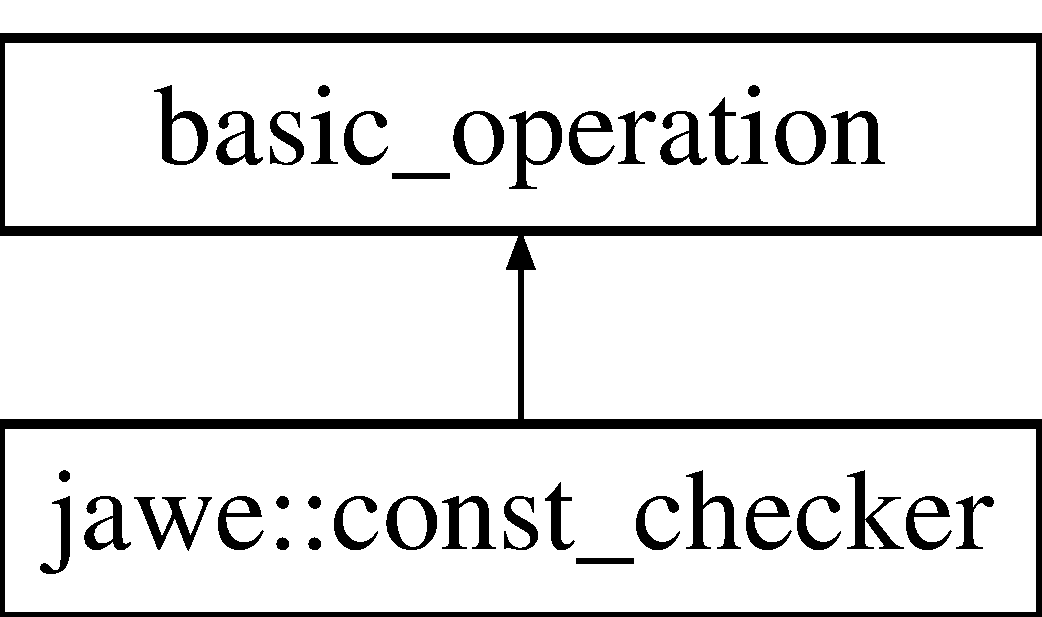
\includegraphics[height=2.000000cm]{classjawe_1_1const__checker}
\end{center}
\end{figure}
\subsection*{Public Member Functions}
\begin{DoxyCompactItemize}
\item 
void \hyperlink{classjawe_1_1const__checker_aa0c7604001ebd8aae5ddab7b52271b47}{run} ()
\end{DoxyCompactItemize}
\subsection*{Private Member Functions}
\begin{DoxyCompactItemize}
\item 
void \hyperlink{classjawe_1_1const__checker_a24bb1b4bee084d3ccd7f8310b6ffed97}{check} (const \hyperlink{namespacejawe_a3f307481d921b6cbb50cc8511fc2b544}{shared\+\_\+node} \&root)
\item 
void \hyperlink{classjawe_1_1const__checker_a4f114db74deafd147266b7677889788e}{print\+\_\+stacks} () const
\item 
std\+::string \hyperlink{classjawe_1_1const__checker_ada31fcc80da323dad6a80d25438c6bdc}{get\+\_\+decl\+\_\+var\+\_\+name} (const \hyperlink{namespacejawe_a3f307481d921b6cbb50cc8511fc2b544}{shared\+\_\+node} \&root)
\end{DoxyCompactItemize}
\subsection*{Private Attributes}
\begin{DoxyCompactItemize}
\item 
\hyperlink{classjawe_1_1utils_1_1scope}{scope}$<$ bool $>$ \hyperlink{classjawe_1_1const__checker_a61092ccd1994ec0075ca03ec39ea4477}{m\+\_\+scopes}
\end{DoxyCompactItemize}


\subsection{Member Function Documentation}
\mbox{\Hypertarget{classjawe_1_1const__checker_a24bb1b4bee084d3ccd7f8310b6ffed97}\label{classjawe_1_1const__checker_a24bb1b4bee084d3ccd7f8310b6ffed97}} 
\index{jawe\+::const\+\_\+checker@{jawe\+::const\+\_\+checker}!check@{check}}
\index{check@{check}!jawe\+::const\+\_\+checker@{jawe\+::const\+\_\+checker}}
\subsubsection{\texorpdfstring{check()}{check()}}
{\footnotesize\ttfamily void const\+\_\+checker\+::check (\begin{DoxyParamCaption}\item[{const \hyperlink{namespacejawe_a3f307481d921b6cbb50cc8511fc2b544}{shared\+\_\+node} \&}]{root }\end{DoxyParamCaption})\hspace{0.3cm}{\ttfamily [private]}}

\mbox{\Hypertarget{classjawe_1_1const__checker_ada31fcc80da323dad6a80d25438c6bdc}\label{classjawe_1_1const__checker_ada31fcc80da323dad6a80d25438c6bdc}} 
\index{jawe\+::const\+\_\+checker@{jawe\+::const\+\_\+checker}!get\+\_\+decl\+\_\+var\+\_\+name@{get\+\_\+decl\+\_\+var\+\_\+name}}
\index{get\+\_\+decl\+\_\+var\+\_\+name@{get\+\_\+decl\+\_\+var\+\_\+name}!jawe\+::const\+\_\+checker@{jawe\+::const\+\_\+checker}}
\subsubsection{\texorpdfstring{get\+\_\+decl\+\_\+var\+\_\+name()}{get\_decl\_var\_name()}}
{\footnotesize\ttfamily std\+::string const\+\_\+checker\+::get\+\_\+decl\+\_\+var\+\_\+name (\begin{DoxyParamCaption}\item[{const \hyperlink{namespacejawe_a3f307481d921b6cbb50cc8511fc2b544}{shared\+\_\+node} \&}]{root }\end{DoxyParamCaption})\hspace{0.3cm}{\ttfamily [private]}}

\mbox{\Hypertarget{classjawe_1_1const__checker_a4f114db74deafd147266b7677889788e}\label{classjawe_1_1const__checker_a4f114db74deafd147266b7677889788e}} 
\index{jawe\+::const\+\_\+checker@{jawe\+::const\+\_\+checker}!print\+\_\+stacks@{print\+\_\+stacks}}
\index{print\+\_\+stacks@{print\+\_\+stacks}!jawe\+::const\+\_\+checker@{jawe\+::const\+\_\+checker}}
\subsubsection{\texorpdfstring{print\+\_\+stacks()}{print\_stacks()}}
{\footnotesize\ttfamily void jawe\+::const\+\_\+checker\+::print\+\_\+stacks (\begin{DoxyParamCaption}{ }\end{DoxyParamCaption}) const\hspace{0.3cm}{\ttfamily [private]}}

\mbox{\Hypertarget{classjawe_1_1const__checker_aa0c7604001ebd8aae5ddab7b52271b47}\label{classjawe_1_1const__checker_aa0c7604001ebd8aae5ddab7b52271b47}} 
\index{jawe\+::const\+\_\+checker@{jawe\+::const\+\_\+checker}!run@{run}}
\index{run@{run}!jawe\+::const\+\_\+checker@{jawe\+::const\+\_\+checker}}
\subsubsection{\texorpdfstring{run()}{run()}}
{\footnotesize\ttfamily void const\+\_\+checker\+::run (\begin{DoxyParamCaption}{ }\end{DoxyParamCaption})}



\subsection{Member Data Documentation}
\mbox{\Hypertarget{classjawe_1_1const__checker_a61092ccd1994ec0075ca03ec39ea4477}\label{classjawe_1_1const__checker_a61092ccd1994ec0075ca03ec39ea4477}} 
\index{jawe\+::const\+\_\+checker@{jawe\+::const\+\_\+checker}!m\+\_\+scopes@{m\+\_\+scopes}}
\index{m\+\_\+scopes@{m\+\_\+scopes}!jawe\+::const\+\_\+checker@{jawe\+::const\+\_\+checker}}
\subsubsection{\texorpdfstring{m\+\_\+scopes}{m\_scopes}}
{\footnotesize\ttfamily \hyperlink{classjawe_1_1utils_1_1scope}{scope}$<$bool$>$ jawe\+::const\+\_\+checker\+::m\+\_\+scopes\hspace{0.3cm}{\ttfamily [private]}}



The documentation for this class was generated from the following files\+:\begin{DoxyCompactItemize}
\item 
include/operations/\hyperlink{const__checker_8hpp}{const\+\_\+checker.\+hpp}\item 
src/operations/\hyperlink{const__checker_8cpp}{const\+\_\+checker.\+cpp}\end{DoxyCompactItemize}

\hypertarget{classjawe_1_1const__declaration__node}{}\section{jawe\+:\+:const\+\_\+declaration\+\_\+node Class Reference}
\label{classjawe_1_1const__declaration__node}\index{jawe\+::const\+\_\+declaration\+\_\+node@{jawe\+::const\+\_\+declaration\+\_\+node}}


{\ttfamily \#include $<$const\+\_\+declaration\+\_\+node.\+hpp$>$}

Inheritance diagram for jawe\+:\+:const\+\_\+declaration\+\_\+node\+:\begin{figure}[H]
\begin{center}
\leavevmode
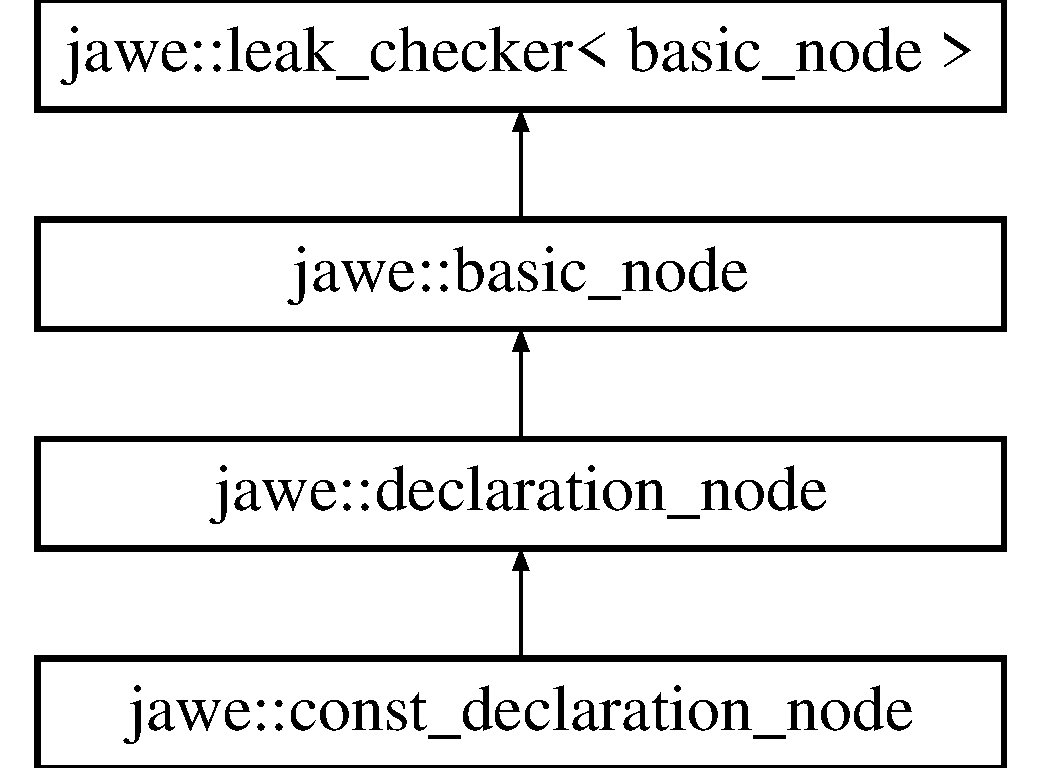
\includegraphics[height=4.000000cm]{classjawe_1_1const__declaration__node}
\end{center}
\end{figure}
\subsection*{Public Member Functions}
\begin{DoxyCompactItemize}
\item 
\hyperlink{classjawe_1_1const__declaration__node_ad31402f724923bf620197ccb175d78f0}{const\+\_\+declaration\+\_\+node} (const \hyperlink{namespacejawe_a3f307481d921b6cbb50cc8511fc2b544}{shared\+\_\+node} \&)
\end{DoxyCompactItemize}
\subsection*{Additional Inherited Members}


\subsection{Constructor \& Destructor Documentation}
\mbox{\Hypertarget{classjawe_1_1const__declaration__node_ad31402f724923bf620197ccb175d78f0}\label{classjawe_1_1const__declaration__node_ad31402f724923bf620197ccb175d78f0}} 
\index{jawe\+::const\+\_\+declaration\+\_\+node@{jawe\+::const\+\_\+declaration\+\_\+node}!const\+\_\+declaration\+\_\+node@{const\+\_\+declaration\+\_\+node}}
\index{const\+\_\+declaration\+\_\+node@{const\+\_\+declaration\+\_\+node}!jawe\+::const\+\_\+declaration\+\_\+node@{jawe\+::const\+\_\+declaration\+\_\+node}}
\subsubsection{\texorpdfstring{const\+\_\+declaration\+\_\+node()}{const\_declaration\_node()}}
{\footnotesize\ttfamily const\+\_\+declaration\+\_\+node\+::const\+\_\+declaration\+\_\+node (\begin{DoxyParamCaption}\item[{const \hyperlink{namespacejawe_a3f307481d921b6cbb50cc8511fc2b544}{shared\+\_\+node} \&}]{shared\+\_\+n }\end{DoxyParamCaption})}



The documentation for this class was generated from the following files\+:\begin{DoxyCompactItemize}
\item 
include/syntax/variables/\hyperlink{const__declaration__node_8hpp}{const\+\_\+declaration\+\_\+node.\+hpp}\item 
src/syntax/variables/\hyperlink{const__declaration__node_8cpp}{const\+\_\+declaration\+\_\+node.\+cpp}\end{DoxyCompactItemize}

\hypertarget{classjawe_1_1continue__node}{}\section{jawe\+:\+:continue\+\_\+node Class Reference}
\label{classjawe_1_1continue__node}\index{jawe\+::continue\+\_\+node@{jawe\+::continue\+\_\+node}}


{\ttfamily \#include $<$continue\+\_\+node.\+hpp$>$}

Inheritance diagram for jawe\+:\+:continue\+\_\+node\+:\begin{figure}[H]
\begin{center}
\leavevmode
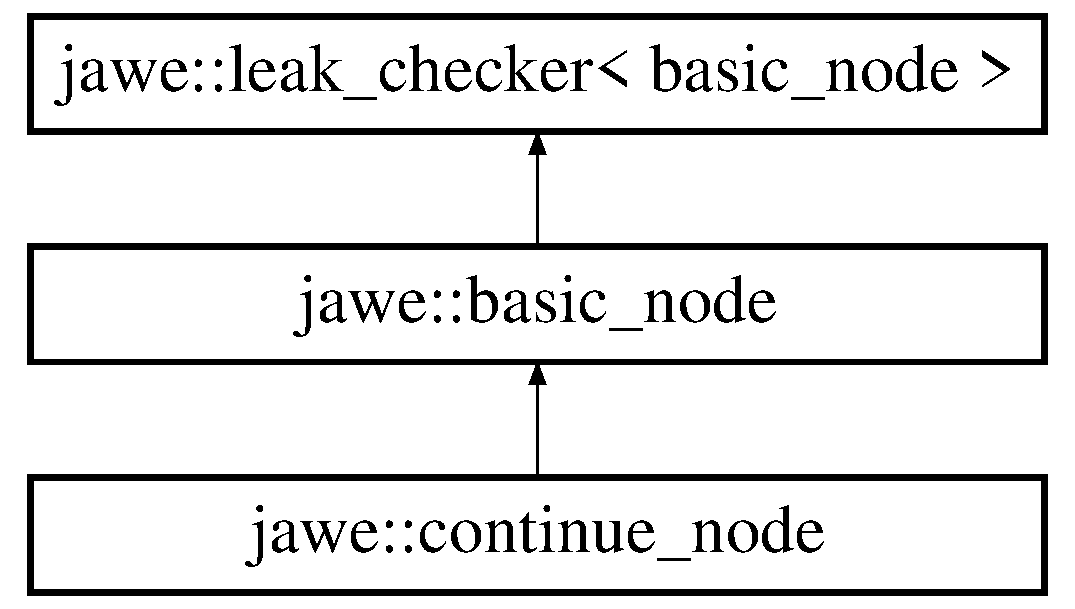
\includegraphics[height=3.000000cm]{classjawe_1_1continue__node}
\end{center}
\end{figure}
\subsection*{Public Member Functions}
\begin{DoxyCompactItemize}
\item 
\hyperlink{classjawe_1_1continue__node_ac9a52325e5f9b5cecb1b8279d7303817}{continue\+\_\+node} ()
\end{DoxyCompactItemize}
\subsection*{Additional Inherited Members}


\subsection{Constructor \& Destructor Documentation}
\mbox{\Hypertarget{classjawe_1_1continue__node_ac9a52325e5f9b5cecb1b8279d7303817}\label{classjawe_1_1continue__node_ac9a52325e5f9b5cecb1b8279d7303817}} 
\index{jawe\+::continue\+\_\+node@{jawe\+::continue\+\_\+node}!continue\+\_\+node@{continue\+\_\+node}}
\index{continue\+\_\+node@{continue\+\_\+node}!jawe\+::continue\+\_\+node@{jawe\+::continue\+\_\+node}}
\subsubsection{\texorpdfstring{continue\+\_\+node()}{continue\_node()}}
{\footnotesize\ttfamily continue\+\_\+node\+::continue\+\_\+node (\begin{DoxyParamCaption}{ }\end{DoxyParamCaption})}



The documentation for this class was generated from the following files\+:\begin{DoxyCompactItemize}
\item 
include/syntax/control\+\_\+flow/\hyperlink{continue__node_8hpp}{continue\+\_\+node.\+hpp}\item 
src/syntax/control\+\_\+flow/\hyperlink{continue__node_8cpp}{continue\+\_\+node.\+cpp}\end{DoxyCompactItemize}

\hypertarget{classjawe_1_1control}{}\section{jawe\+:\+:control Class Reference}
\label{classjawe_1_1control}\index{jawe\+::control@{jawe\+::control}}


Singleton class that manages the state of compiler.  




{\ttfamily \#include $<$control.\+hpp$>$}

\subsection*{Public Member Functions}
\begin{DoxyCompactItemize}
\item 
\hyperlink{classjawe_1_1control_a389d474b7c44f71337414bc0654be440}{control} (const \hyperlink{classjawe_1_1control}{control} \&)=delete
\item 
void \hyperlink{classjawe_1_1control_ae93188db9e9ff6f31820b65338170743}{operator=} (const \hyperlink{classjawe_1_1control}{control} \&)=delete
\item 
std\+::string \hyperlink{classjawe_1_1control_adba7db777afd24542c7964b37c40ddd9}{input\+\_\+filename} () const
\item 
bool \hyperlink{classjawe_1_1control_af6b03624889bba5b03ec0c2587dfcb0a}{dump\+\_\+ast} () const
\item 
bool \hyperlink{classjawe_1_1control_ad13168abb7f48d6e748a4f13f45db5b4}{dump\+\_\+program} () const
\item 
bool \hyperlink{classjawe_1_1control_a2e83d269a8836025b9f825beef846fe7}{dump\+\_\+ir} () const
\item 
bool \hyperlink{classjawe_1_1control_a504da571a1eeb32bf9c9b5957dca5ae1}{show\+\_\+memory} () const
\item 
bool \hyperlink{classjawe_1_1control_a3770ef7a1572ac8d25f30785d04c4e1a}{check\+\_\+leaks} () const
\item 
llvm\+::\+L\+L\+V\+M\+Context \& \hyperlink{classjawe_1_1control_a77eced5b2483f1d9b3f95d8137f2e8b6}{get\+\_\+context} ()
\item 
std\+::unique\+\_\+ptr$<$ llvm\+::\+Module $>$ \& \hyperlink{classjawe_1_1control_ab332f27bb37743e03c9e61ddc93da26c}{get\+\_\+module} ()
\item 
void \hyperlink{classjawe_1_1control_aedf6bf138a9ef62d589458b65f62eae5}{run} () const
\end{DoxyCompactItemize}
\subsection*{Static Public Member Functions}
\begin{DoxyCompactItemize}
\item 
static \hyperlink{classjawe_1_1control}{control} \& \hyperlink{classjawe_1_1control_ad702fe6d2f641c518d12665278df20a3}{get} (int argc=0, char $\ast$$\ast$argv=nullptr)
\begin{DoxyCompactList}\small\item\em Gets singleton instance. \end{DoxyCompactList}\end{DoxyCompactItemize}
\subsection*{Private Member Functions}
\begin{DoxyCompactItemize}
\item 
\hyperlink{classjawe_1_1control_abaa77c23608e1eec0077bc9e4ae1554c}{control} (int argc, char $\ast$$\ast$argv)
\begin{DoxyCompactList}\small\item\em Constructs control (singleton) instance. \end{DoxyCompactList}\item 
void \hyperlink{classjawe_1_1control_ab5a7e27e96ce6489a1cd3f858ebee6c3}{m\+\_\+print\+\_\+help} () const
\item 
void \hyperlink{classjawe_1_1control_a6142361ac84b3a77c41b6137d8dfcc6f}{m\+\_\+print\+\_\+version} () const
\end{DoxyCompactItemize}
\subsection*{Private Attributes}
\begin{DoxyCompactItemize}
\item 
int \hyperlink{classjawe_1_1control_a3e68b0df0786c7d69313e870f991d34a}{m\+\_\+argc}
\item 
char $\ast$$\ast$ \hyperlink{classjawe_1_1control_a1449ae95dcbd6fb6fee97bc28d38e246}{m\+\_\+argv}
\item 
boost\+::program\+\_\+options\+::options\+\_\+description \hyperlink{classjawe_1_1control_a7e86c44df163e1991167626e7e3e32d5}{m\+\_\+desc}
\item 
boost\+::program\+\_\+options\+::variables\+\_\+map \hyperlink{classjawe_1_1control_ada42ec370e2de6b2473e76efffaf25af}{m\+\_\+vars}
\item 
std\+::string \hyperlink{classjawe_1_1control_ad13652c476203209baef18476bb0ca8d}{m\+\_\+input}
\item 
std\+::string \hyperlink{classjawe_1_1control_a3847da990d053ee84fe7b66847e66cda}{m\+\_\+output}
\item 
bool \hyperlink{classjawe_1_1control_a993a9e6eff6a143ef985083c57ae267b}{m\+\_\+dump\+\_\+ast}
\item 
bool \hyperlink{classjawe_1_1control_acc4256916f57b4c8721fa24d8c15f3b5}{m\+\_\+dump\+\_\+program}
\item 
bool \hyperlink{classjawe_1_1control_a216a5071cb4effe06bc36216c61e55c1}{m\+\_\+dump\+\_\+ir}
\item 
bool \hyperlink{classjawe_1_1control_acaf44d403cbccc7d16f514c5c0dcceed}{m\+\_\+show\+\_\+memory}
\item 
bool \hyperlink{classjawe_1_1control_a91b200a38784da33881a0692925db04e}{m\+\_\+check\+\_\+leaks}
\item 
llvm\+::\+L\+L\+V\+M\+Context \hyperlink{classjawe_1_1control_aa996f999ce396f57e18448d06bd46a14}{m\+\_\+context}
\item 
std\+::unique\+\_\+ptr$<$ llvm\+::\+Module $>$ \hyperlink{classjawe_1_1control_a86b9aa016d912fd00d08bc1b9597839f}{m\+\_\+module}
\end{DoxyCompactItemize}


\subsection{Detailed Description}
Singleton class that manages the state of compiler. 

It\textquotesingle{} primarily purpose is to manage the state, run the steps, and to set the flags that are passed when running the compiler. Also, it is the owner of L\+L\+VM module and context. 

\subsection{Constructor \& Destructor Documentation}
\mbox{\Hypertarget{classjawe_1_1control_a389d474b7c44f71337414bc0654be440}\label{classjawe_1_1control_a389d474b7c44f71337414bc0654be440}} 
\index{jawe\+::control@{jawe\+::control}!control@{control}}
\index{control@{control}!jawe\+::control@{jawe\+::control}}
\subsubsection{\texorpdfstring{control()}{control()}\hspace{0.1cm}{\footnotesize\ttfamily [1/2]}}
{\footnotesize\ttfamily jawe\+::control\+::control (\begin{DoxyParamCaption}\item[{const \hyperlink{classjawe_1_1control}{control} \&}]{ }\end{DoxyParamCaption})\hspace{0.3cm}{\ttfamily [delete]}}

Deleted copy constructor. Prevention against copying singleton instance. \mbox{\Hypertarget{classjawe_1_1control_abaa77c23608e1eec0077bc9e4ae1554c}\label{classjawe_1_1control_abaa77c23608e1eec0077bc9e4ae1554c}} 
\index{jawe\+::control@{jawe\+::control}!control@{control}}
\index{control@{control}!jawe\+::control@{jawe\+::control}}
\subsubsection{\texorpdfstring{control()}{control()}\hspace{0.1cm}{\footnotesize\ttfamily [2/2]}}
{\footnotesize\ttfamily control\+::control (\begin{DoxyParamCaption}\item[{int}]{argc,  }\item[{char $\ast$$\ast$}]{argv }\end{DoxyParamCaption})\hspace{0.3cm}{\ttfamily [private]}}



Constructs control (singleton) instance. 

This constructor is used when first creating an instance. It accepts command line arguments so that they can be passed to boost\+::program\+\_\+options library. 
\begin{DoxyParams}{Parameters}
{\em argc} & number of command line arguments. \\
\hline
{\em argv} & an array of strings (command line arguments) \\
\hline
\end{DoxyParams}


\subsection{Member Function Documentation}
\mbox{\Hypertarget{classjawe_1_1control_a3770ef7a1572ac8d25f30785d04c4e1a}\label{classjawe_1_1control_a3770ef7a1572ac8d25f30785d04c4e1a}} 
\index{jawe\+::control@{jawe\+::control}!check\+\_\+leaks@{check\+\_\+leaks}}
\index{check\+\_\+leaks@{check\+\_\+leaks}!jawe\+::control@{jawe\+::control}}
\subsubsection{\texorpdfstring{check\+\_\+leaks()}{check\_leaks()}}
{\footnotesize\ttfamily bool control\+::check\+\_\+leaks (\begin{DoxyParamCaption}{ }\end{DoxyParamCaption}) const}

Checks if --check-\/leaks flag is passed. \mbox{\Hypertarget{classjawe_1_1control_af6b03624889bba5b03ec0c2587dfcb0a}\label{classjawe_1_1control_af6b03624889bba5b03ec0c2587dfcb0a}} 
\index{jawe\+::control@{jawe\+::control}!dump\+\_\+ast@{dump\+\_\+ast}}
\index{dump\+\_\+ast@{dump\+\_\+ast}!jawe\+::control@{jawe\+::control}}
\subsubsection{\texorpdfstring{dump\+\_\+ast()}{dump\_ast()}}
{\footnotesize\ttfamily bool control\+::dump\+\_\+ast (\begin{DoxyParamCaption}{ }\end{DoxyParamCaption}) const}

Checks if --dump-\/ast flag is passed. \mbox{\Hypertarget{classjawe_1_1control_a2e83d269a8836025b9f825beef846fe7}\label{classjawe_1_1control_a2e83d269a8836025b9f825beef846fe7}} 
\index{jawe\+::control@{jawe\+::control}!dump\+\_\+ir@{dump\+\_\+ir}}
\index{dump\+\_\+ir@{dump\+\_\+ir}!jawe\+::control@{jawe\+::control}}
\subsubsection{\texorpdfstring{dump\+\_\+ir()}{dump\_ir()}}
{\footnotesize\ttfamily bool control\+::dump\+\_\+ir (\begin{DoxyParamCaption}{ }\end{DoxyParamCaption}) const}

Checks if --dump-\/ir flag is passed. \mbox{\Hypertarget{classjawe_1_1control_ad13168abb7f48d6e748a4f13f45db5b4}\label{classjawe_1_1control_ad13168abb7f48d6e748a4f13f45db5b4}} 
\index{jawe\+::control@{jawe\+::control}!dump\+\_\+program@{dump\+\_\+program}}
\index{dump\+\_\+program@{dump\+\_\+program}!jawe\+::control@{jawe\+::control}}
\subsubsection{\texorpdfstring{dump\+\_\+program()}{dump\_program()}}
{\footnotesize\ttfamily bool control\+::dump\+\_\+program (\begin{DoxyParamCaption}{ }\end{DoxyParamCaption}) const}

Checks if --dump-\/program flag is passed. \mbox{\Hypertarget{classjawe_1_1control_ad702fe6d2f641c518d12665278df20a3}\label{classjawe_1_1control_ad702fe6d2f641c518d12665278df20a3}} 
\index{jawe\+::control@{jawe\+::control}!get@{get}}
\index{get@{get}!jawe\+::control@{jawe\+::control}}
\subsubsection{\texorpdfstring{get()}{get()}}
{\footnotesize\ttfamily \hyperlink{classjawe_1_1control}{control} \& control\+::get (\begin{DoxyParamCaption}\item[{int}]{argc = {\ttfamily 0},  }\item[{char $\ast$$\ast$}]{argv = {\ttfamily nullptr} }\end{DoxyParamCaption})\hspace{0.3cm}{\ttfamily [static]}}



Gets singleton instance. 

Command line arguments must be passed in order to construct the original instance. Once constructed, these arguments become obsolete, and should not be passed again. 
\begin{DoxyParams}{Parameters}
{\em argc} & number of command line arguments. \\
\hline
{\em argv} & an array of strings (command line arguments) \\
\hline
\end{DoxyParams}
\mbox{\Hypertarget{classjawe_1_1control_a77eced5b2483f1d9b3f95d8137f2e8b6}\label{classjawe_1_1control_a77eced5b2483f1d9b3f95d8137f2e8b6}} 
\index{jawe\+::control@{jawe\+::control}!get\+\_\+context@{get\+\_\+context}}
\index{get\+\_\+context@{get\+\_\+context}!jawe\+::control@{jawe\+::control}}
\subsubsection{\texorpdfstring{get\+\_\+context()}{get\_context()}}
{\footnotesize\ttfamily llvm\+::\+L\+L\+V\+M\+Context \& control\+::get\+\_\+context (\begin{DoxyParamCaption}{ }\end{DoxyParamCaption})}

Gets L\+L\+VM context. \mbox{\Hypertarget{classjawe_1_1control_ab332f27bb37743e03c9e61ddc93da26c}\label{classjawe_1_1control_ab332f27bb37743e03c9e61ddc93da26c}} 
\index{jawe\+::control@{jawe\+::control}!get\+\_\+module@{get\+\_\+module}}
\index{get\+\_\+module@{get\+\_\+module}!jawe\+::control@{jawe\+::control}}
\subsubsection{\texorpdfstring{get\+\_\+module()}{get\_module()}}
{\footnotesize\ttfamily std\+::unique\+\_\+ptr$<$ llvm\+::\+Module $>$ \& control\+::get\+\_\+module (\begin{DoxyParamCaption}{ }\end{DoxyParamCaption})}

Gets pointer to L\+L\+VM module. \mbox{\Hypertarget{classjawe_1_1control_adba7db777afd24542c7964b37c40ddd9}\label{classjawe_1_1control_adba7db777afd24542c7964b37c40ddd9}} 
\index{jawe\+::control@{jawe\+::control}!input\+\_\+filename@{input\+\_\+filename}}
\index{input\+\_\+filename@{input\+\_\+filename}!jawe\+::control@{jawe\+::control}}
\subsubsection{\texorpdfstring{input\+\_\+filename()}{input\_filename()}}
{\footnotesize\ttfamily std\+::string control\+::input\+\_\+filename (\begin{DoxyParamCaption}{ }\end{DoxyParamCaption}) const}

Gets the filename (path) of the input file. \mbox{\Hypertarget{classjawe_1_1control_ab5a7e27e96ce6489a1cd3f858ebee6c3}\label{classjawe_1_1control_ab5a7e27e96ce6489a1cd3f858ebee6c3}} 
\index{jawe\+::control@{jawe\+::control}!m\+\_\+print\+\_\+help@{m\+\_\+print\+\_\+help}}
\index{m\+\_\+print\+\_\+help@{m\+\_\+print\+\_\+help}!jawe\+::control@{jawe\+::control}}
\subsubsection{\texorpdfstring{m\+\_\+print\+\_\+help()}{m\_print\_help()}}
{\footnotesize\ttfamily void control\+::m\+\_\+print\+\_\+help (\begin{DoxyParamCaption}{ }\end{DoxyParamCaption}) const\hspace{0.3cm}{\ttfamily [private]}}

Prints help message (gets called if --help flag is set) \mbox{\Hypertarget{classjawe_1_1control_a6142361ac84b3a77c41b6137d8dfcc6f}\label{classjawe_1_1control_a6142361ac84b3a77c41b6137d8dfcc6f}} 
\index{jawe\+::control@{jawe\+::control}!m\+\_\+print\+\_\+version@{m\+\_\+print\+\_\+version}}
\index{m\+\_\+print\+\_\+version@{m\+\_\+print\+\_\+version}!jawe\+::control@{jawe\+::control}}
\subsubsection{\texorpdfstring{m\+\_\+print\+\_\+version()}{m\_print\_version()}}
{\footnotesize\ttfamily void control\+::m\+\_\+print\+\_\+version (\begin{DoxyParamCaption}{ }\end{DoxyParamCaption}) const\hspace{0.3cm}{\ttfamily [private]}}

Prints version message (gets called if --version flag is set) \mbox{\Hypertarget{classjawe_1_1control_ae93188db9e9ff6f31820b65338170743}\label{classjawe_1_1control_ae93188db9e9ff6f31820b65338170743}} 
\index{jawe\+::control@{jawe\+::control}!operator=@{operator=}}
\index{operator=@{operator=}!jawe\+::control@{jawe\+::control}}
\subsubsection{\texorpdfstring{operator=()}{operator=()}}
{\footnotesize\ttfamily void jawe\+::control\+::operator= (\begin{DoxyParamCaption}\item[{const \hyperlink{classjawe_1_1control}{control} \&}]{ }\end{DoxyParamCaption})\hspace{0.3cm}{\ttfamily [delete]}}

Deleted copy assignment operator. Prevention against copying singleton instance. \mbox{\Hypertarget{classjawe_1_1control_aedf6bf138a9ef62d589458b65f62eae5}\label{classjawe_1_1control_aedf6bf138a9ef62d589458b65f62eae5}} 
\index{jawe\+::control@{jawe\+::control}!run@{run}}
\index{run@{run}!jawe\+::control@{jawe\+::control}}
\subsubsection{\texorpdfstring{run()}{run()}}
{\footnotesize\ttfamily void control\+::run (\begin{DoxyParamCaption}{ }\end{DoxyParamCaption}) const}

Starts all the phases of compiler. \mbox{\Hypertarget{classjawe_1_1control_a504da571a1eeb32bf9c9b5957dca5ae1}\label{classjawe_1_1control_a504da571a1eeb32bf9c9b5957dca5ae1}} 
\index{jawe\+::control@{jawe\+::control}!show\+\_\+memory@{show\+\_\+memory}}
\index{show\+\_\+memory@{show\+\_\+memory}!jawe\+::control@{jawe\+::control}}
\subsubsection{\texorpdfstring{show\+\_\+memory()}{show\_memory()}}
{\footnotesize\ttfamily bool control\+::show\+\_\+memory (\begin{DoxyParamCaption}{ }\end{DoxyParamCaption}) const}

Checks if --show-\/memory flag is passed. 

\subsection{Member Data Documentation}
\mbox{\Hypertarget{classjawe_1_1control_a3e68b0df0786c7d69313e870f991d34a}\label{classjawe_1_1control_a3e68b0df0786c7d69313e870f991d34a}} 
\index{jawe\+::control@{jawe\+::control}!m\+\_\+argc@{m\+\_\+argc}}
\index{m\+\_\+argc@{m\+\_\+argc}!jawe\+::control@{jawe\+::control}}
\subsubsection{\texorpdfstring{m\+\_\+argc}{m\_argc}}
{\footnotesize\ttfamily int jawe\+::control\+::m\+\_\+argc\hspace{0.3cm}{\ttfamily [private]}}

\mbox{\Hypertarget{classjawe_1_1control_a1449ae95dcbd6fb6fee97bc28d38e246}\label{classjawe_1_1control_a1449ae95dcbd6fb6fee97bc28d38e246}} 
\index{jawe\+::control@{jawe\+::control}!m\+\_\+argv@{m\+\_\+argv}}
\index{m\+\_\+argv@{m\+\_\+argv}!jawe\+::control@{jawe\+::control}}
\subsubsection{\texorpdfstring{m\+\_\+argv}{m\_argv}}
{\footnotesize\ttfamily char$\ast$$\ast$ jawe\+::control\+::m\+\_\+argv\hspace{0.3cm}{\ttfamily [private]}}

\mbox{\Hypertarget{classjawe_1_1control_a91b200a38784da33881a0692925db04e}\label{classjawe_1_1control_a91b200a38784da33881a0692925db04e}} 
\index{jawe\+::control@{jawe\+::control}!m\+\_\+check\+\_\+leaks@{m\+\_\+check\+\_\+leaks}}
\index{m\+\_\+check\+\_\+leaks@{m\+\_\+check\+\_\+leaks}!jawe\+::control@{jawe\+::control}}
\subsubsection{\texorpdfstring{m\+\_\+check\+\_\+leaks}{m\_check\_leaks}}
{\footnotesize\ttfamily bool jawe\+::control\+::m\+\_\+check\+\_\+leaks\hspace{0.3cm}{\ttfamily [private]}}

\mbox{\Hypertarget{classjawe_1_1control_aa996f999ce396f57e18448d06bd46a14}\label{classjawe_1_1control_aa996f999ce396f57e18448d06bd46a14}} 
\index{jawe\+::control@{jawe\+::control}!m\+\_\+context@{m\+\_\+context}}
\index{m\+\_\+context@{m\+\_\+context}!jawe\+::control@{jawe\+::control}}
\subsubsection{\texorpdfstring{m\+\_\+context}{m\_context}}
{\footnotesize\ttfamily llvm\+::\+L\+L\+V\+M\+Context jawe\+::control\+::m\+\_\+context\hspace{0.3cm}{\ttfamily [private]}}

\mbox{\Hypertarget{classjawe_1_1control_a7e86c44df163e1991167626e7e3e32d5}\label{classjawe_1_1control_a7e86c44df163e1991167626e7e3e32d5}} 
\index{jawe\+::control@{jawe\+::control}!m\+\_\+desc@{m\+\_\+desc}}
\index{m\+\_\+desc@{m\+\_\+desc}!jawe\+::control@{jawe\+::control}}
\subsubsection{\texorpdfstring{m\+\_\+desc}{m\_desc}}
{\footnotesize\ttfamily boost\+::program\+\_\+options\+::options\+\_\+description jawe\+::control\+::m\+\_\+desc\hspace{0.3cm}{\ttfamily [private]}}

\mbox{\Hypertarget{classjawe_1_1control_a993a9e6eff6a143ef985083c57ae267b}\label{classjawe_1_1control_a993a9e6eff6a143ef985083c57ae267b}} 
\index{jawe\+::control@{jawe\+::control}!m\+\_\+dump\+\_\+ast@{m\+\_\+dump\+\_\+ast}}
\index{m\+\_\+dump\+\_\+ast@{m\+\_\+dump\+\_\+ast}!jawe\+::control@{jawe\+::control}}
\subsubsection{\texorpdfstring{m\+\_\+dump\+\_\+ast}{m\_dump\_ast}}
{\footnotesize\ttfamily bool jawe\+::control\+::m\+\_\+dump\+\_\+ast\hspace{0.3cm}{\ttfamily [private]}}

\mbox{\Hypertarget{classjawe_1_1control_a216a5071cb4effe06bc36216c61e55c1}\label{classjawe_1_1control_a216a5071cb4effe06bc36216c61e55c1}} 
\index{jawe\+::control@{jawe\+::control}!m\+\_\+dump\+\_\+ir@{m\+\_\+dump\+\_\+ir}}
\index{m\+\_\+dump\+\_\+ir@{m\+\_\+dump\+\_\+ir}!jawe\+::control@{jawe\+::control}}
\subsubsection{\texorpdfstring{m\+\_\+dump\+\_\+ir}{m\_dump\_ir}}
{\footnotesize\ttfamily bool jawe\+::control\+::m\+\_\+dump\+\_\+ir\hspace{0.3cm}{\ttfamily [private]}}

\mbox{\Hypertarget{classjawe_1_1control_acc4256916f57b4c8721fa24d8c15f3b5}\label{classjawe_1_1control_acc4256916f57b4c8721fa24d8c15f3b5}} 
\index{jawe\+::control@{jawe\+::control}!m\+\_\+dump\+\_\+program@{m\+\_\+dump\+\_\+program}}
\index{m\+\_\+dump\+\_\+program@{m\+\_\+dump\+\_\+program}!jawe\+::control@{jawe\+::control}}
\subsubsection{\texorpdfstring{m\+\_\+dump\+\_\+program}{m\_dump\_program}}
{\footnotesize\ttfamily bool jawe\+::control\+::m\+\_\+dump\+\_\+program\hspace{0.3cm}{\ttfamily [private]}}

\mbox{\Hypertarget{classjawe_1_1control_ad13652c476203209baef18476bb0ca8d}\label{classjawe_1_1control_ad13652c476203209baef18476bb0ca8d}} 
\index{jawe\+::control@{jawe\+::control}!m\+\_\+input@{m\+\_\+input}}
\index{m\+\_\+input@{m\+\_\+input}!jawe\+::control@{jawe\+::control}}
\subsubsection{\texorpdfstring{m\+\_\+input}{m\_input}}
{\footnotesize\ttfamily std\+::string jawe\+::control\+::m\+\_\+input\hspace{0.3cm}{\ttfamily [private]}}

\mbox{\Hypertarget{classjawe_1_1control_a86b9aa016d912fd00d08bc1b9597839f}\label{classjawe_1_1control_a86b9aa016d912fd00d08bc1b9597839f}} 
\index{jawe\+::control@{jawe\+::control}!m\+\_\+module@{m\+\_\+module}}
\index{m\+\_\+module@{m\+\_\+module}!jawe\+::control@{jawe\+::control}}
\subsubsection{\texorpdfstring{m\+\_\+module}{m\_module}}
{\footnotesize\ttfamily std\+::unique\+\_\+ptr$<$llvm\+::\+Module$>$ jawe\+::control\+::m\+\_\+module\hspace{0.3cm}{\ttfamily [private]}}

\mbox{\Hypertarget{classjawe_1_1control_a3847da990d053ee84fe7b66847e66cda}\label{classjawe_1_1control_a3847da990d053ee84fe7b66847e66cda}} 
\index{jawe\+::control@{jawe\+::control}!m\+\_\+output@{m\+\_\+output}}
\index{m\+\_\+output@{m\+\_\+output}!jawe\+::control@{jawe\+::control}}
\subsubsection{\texorpdfstring{m\+\_\+output}{m\_output}}
{\footnotesize\ttfamily std\+::string jawe\+::control\+::m\+\_\+output\hspace{0.3cm}{\ttfamily [private]}}

\mbox{\Hypertarget{classjawe_1_1control_acaf44d403cbccc7d16f514c5c0dcceed}\label{classjawe_1_1control_acaf44d403cbccc7d16f514c5c0dcceed}} 
\index{jawe\+::control@{jawe\+::control}!m\+\_\+show\+\_\+memory@{m\+\_\+show\+\_\+memory}}
\index{m\+\_\+show\+\_\+memory@{m\+\_\+show\+\_\+memory}!jawe\+::control@{jawe\+::control}}
\subsubsection{\texorpdfstring{m\+\_\+show\+\_\+memory}{m\_show\_memory}}
{\footnotesize\ttfamily bool jawe\+::control\+::m\+\_\+show\+\_\+memory\hspace{0.3cm}{\ttfamily [private]}}

\mbox{\Hypertarget{classjawe_1_1control_ada42ec370e2de6b2473e76efffaf25af}\label{classjawe_1_1control_ada42ec370e2de6b2473e76efffaf25af}} 
\index{jawe\+::control@{jawe\+::control}!m\+\_\+vars@{m\+\_\+vars}}
\index{m\+\_\+vars@{m\+\_\+vars}!jawe\+::control@{jawe\+::control}}
\subsubsection{\texorpdfstring{m\+\_\+vars}{m\_vars}}
{\footnotesize\ttfamily boost\+::program\+\_\+options\+::variables\+\_\+map jawe\+::control\+::m\+\_\+vars\hspace{0.3cm}{\ttfamily [private]}}



The documentation for this class was generated from the following files\+:\begin{DoxyCompactItemize}
\item 
include/utils/\hyperlink{control_8hpp}{control.\+hpp}\item 
src/utils/\hyperlink{control_8cpp}{control.\+cpp}\end{DoxyCompactItemize}

\hypertarget{classjawe_1_1declaration__node}{}\section{jawe\+:\+:declaration\+\_\+node Class Reference}
\label{classjawe_1_1declaration__node}\index{jawe\+::declaration\+\_\+node@{jawe\+::declaration\+\_\+node}}


{\ttfamily \#include $<$declaration\+\_\+node.\+hpp$>$}

Inheritance diagram for jawe\+:\+:declaration\+\_\+node\+:\begin{figure}[H]
\begin{center}
\leavevmode
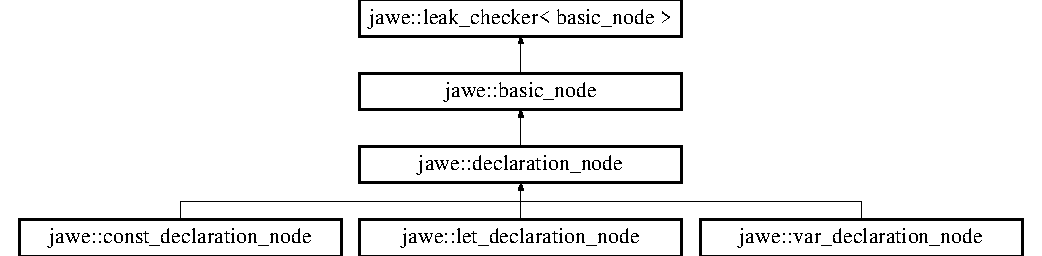
\includegraphics[height=3.440860cm]{classjawe_1_1declaration__node}
\end{center}
\end{figure}
\subsection*{Public Member Functions}
\begin{DoxyCompactItemize}
\item 
\hyperlink{classjawe_1_1declaration__node_af927c96ffda696812f1abd3be57e7160}{declaration\+\_\+node} (const \hyperlink{namespacejawe_a3f307481d921b6cbb50cc8511fc2b544}{shared\+\_\+node} \&, \hyperlink{namespacejawe_aeebd1dfc752b79ba7f0483883a839a1e}{qualifier}, std\+::string)
\item 
\hyperlink{namespacejawe_aeebd1dfc752b79ba7f0483883a839a1e}{qualifier} \hyperlink{classjawe_1_1declaration__node_a55b9f60f34d212df4ee7e2a96a372d1f}{get\+\_\+qualifier} () const
\item 
\hyperlink{namespacejawe_a3f307481d921b6cbb50cc8511fc2b544}{shared\+\_\+node} \hyperlink{classjawe_1_1declaration__node_a8563061c0c3048adabb08cfcc9e0c83b}{get\+\_\+expr} () const
\end{DoxyCompactItemize}
\subsection*{Private Attributes}
\begin{DoxyCompactItemize}
\item 
\hyperlink{namespacejawe_a3f307481d921b6cbb50cc8511fc2b544}{shared\+\_\+node} \hyperlink{classjawe_1_1declaration__node_a07f4d07f9c057ae5ea2591894b447911}{m\+\_\+expr}
\item 
\hyperlink{namespacejawe_aeebd1dfc752b79ba7f0483883a839a1e}{qualifier} \hyperlink{classjawe_1_1declaration__node_aa5647d8c9d733c66d4a9d22486a3b026}{m\+\_\+qualifier}
\end{DoxyCompactItemize}
\subsection*{Additional Inherited Members}


\subsection{Constructor \& Destructor Documentation}
\mbox{\Hypertarget{classjawe_1_1declaration__node_af927c96ffda696812f1abd3be57e7160}\label{classjawe_1_1declaration__node_af927c96ffda696812f1abd3be57e7160}} 
\index{jawe\+::declaration\+\_\+node@{jawe\+::declaration\+\_\+node}!declaration\+\_\+node@{declaration\+\_\+node}}
\index{declaration\+\_\+node@{declaration\+\_\+node}!jawe\+::declaration\+\_\+node@{jawe\+::declaration\+\_\+node}}
\subsubsection{\texorpdfstring{declaration\+\_\+node()}{declaration\_node()}}
{\footnotesize\ttfamily declaration\+\_\+node\+::declaration\+\_\+node (\begin{DoxyParamCaption}\item[{const \hyperlink{namespacejawe_a3f307481d921b6cbb50cc8511fc2b544}{shared\+\_\+node} \&}]{node,  }\item[{\hyperlink{namespacejawe_aeebd1dfc752b79ba7f0483883a839a1e}{qualifier}}]{qualif,  }\item[{std\+::string}]{symbol }\end{DoxyParamCaption})}



\subsection{Member Function Documentation}
\mbox{\Hypertarget{classjawe_1_1declaration__node_a8563061c0c3048adabb08cfcc9e0c83b}\label{classjawe_1_1declaration__node_a8563061c0c3048adabb08cfcc9e0c83b}} 
\index{jawe\+::declaration\+\_\+node@{jawe\+::declaration\+\_\+node}!get\+\_\+expr@{get\+\_\+expr}}
\index{get\+\_\+expr@{get\+\_\+expr}!jawe\+::declaration\+\_\+node@{jawe\+::declaration\+\_\+node}}
\subsubsection{\texorpdfstring{get\+\_\+expr()}{get\_expr()}}
{\footnotesize\ttfamily \hyperlink{namespacejawe_a3f307481d921b6cbb50cc8511fc2b544}{shared\+\_\+node} declaration\+\_\+node\+::get\+\_\+expr (\begin{DoxyParamCaption}{ }\end{DoxyParamCaption}) const}

\mbox{\Hypertarget{classjawe_1_1declaration__node_a55b9f60f34d212df4ee7e2a96a372d1f}\label{classjawe_1_1declaration__node_a55b9f60f34d212df4ee7e2a96a372d1f}} 
\index{jawe\+::declaration\+\_\+node@{jawe\+::declaration\+\_\+node}!get\+\_\+qualifier@{get\+\_\+qualifier}}
\index{get\+\_\+qualifier@{get\+\_\+qualifier}!jawe\+::declaration\+\_\+node@{jawe\+::declaration\+\_\+node}}
\subsubsection{\texorpdfstring{get\+\_\+qualifier()}{get\_qualifier()}}
{\footnotesize\ttfamily \hyperlink{namespacejawe_aeebd1dfc752b79ba7f0483883a839a1e}{qualifier} declaration\+\_\+node\+::get\+\_\+qualifier (\begin{DoxyParamCaption}{ }\end{DoxyParamCaption}) const}



\subsection{Member Data Documentation}
\mbox{\Hypertarget{classjawe_1_1declaration__node_a07f4d07f9c057ae5ea2591894b447911}\label{classjawe_1_1declaration__node_a07f4d07f9c057ae5ea2591894b447911}} 
\index{jawe\+::declaration\+\_\+node@{jawe\+::declaration\+\_\+node}!m\+\_\+expr@{m\+\_\+expr}}
\index{m\+\_\+expr@{m\+\_\+expr}!jawe\+::declaration\+\_\+node@{jawe\+::declaration\+\_\+node}}
\subsubsection{\texorpdfstring{m\+\_\+expr}{m\_expr}}
{\footnotesize\ttfamily \hyperlink{namespacejawe_a3f307481d921b6cbb50cc8511fc2b544}{shared\+\_\+node} jawe\+::declaration\+\_\+node\+::m\+\_\+expr\hspace{0.3cm}{\ttfamily [private]}}

\mbox{\Hypertarget{classjawe_1_1declaration__node_aa5647d8c9d733c66d4a9d22486a3b026}\label{classjawe_1_1declaration__node_aa5647d8c9d733c66d4a9d22486a3b026}} 
\index{jawe\+::declaration\+\_\+node@{jawe\+::declaration\+\_\+node}!m\+\_\+qualifier@{m\+\_\+qualifier}}
\index{m\+\_\+qualifier@{m\+\_\+qualifier}!jawe\+::declaration\+\_\+node@{jawe\+::declaration\+\_\+node}}
\subsubsection{\texorpdfstring{m\+\_\+qualifier}{m\_qualifier}}
{\footnotesize\ttfamily \hyperlink{namespacejawe_aeebd1dfc752b79ba7f0483883a839a1e}{qualifier} jawe\+::declaration\+\_\+node\+::m\+\_\+qualifier\hspace{0.3cm}{\ttfamily [private]}}



The documentation for this class was generated from the following files\+:\begin{DoxyCompactItemize}
\item 
include/syntax/variables/\hyperlink{declaration__node_8hpp}{declaration\+\_\+node.\+hpp}\item 
src/syntax/variables/\hyperlink{declaration__node_8cpp}{declaration\+\_\+node.\+cpp}\end{DoxyCompactItemize}

\hypertarget{classjawe_1_1decrement__node}{}\section{jawe\+:\+:decrement\+\_\+node Class Reference}
\label{classjawe_1_1decrement__node}\index{jawe\+::decrement\+\_\+node@{jawe\+::decrement\+\_\+node}}


{\ttfamily \#include $<$decrement\+\_\+node.\+hpp$>$}

Inheritance diagram for jawe\+:\+:decrement\+\_\+node\+:\begin{figure}[H]
\begin{center}
\leavevmode
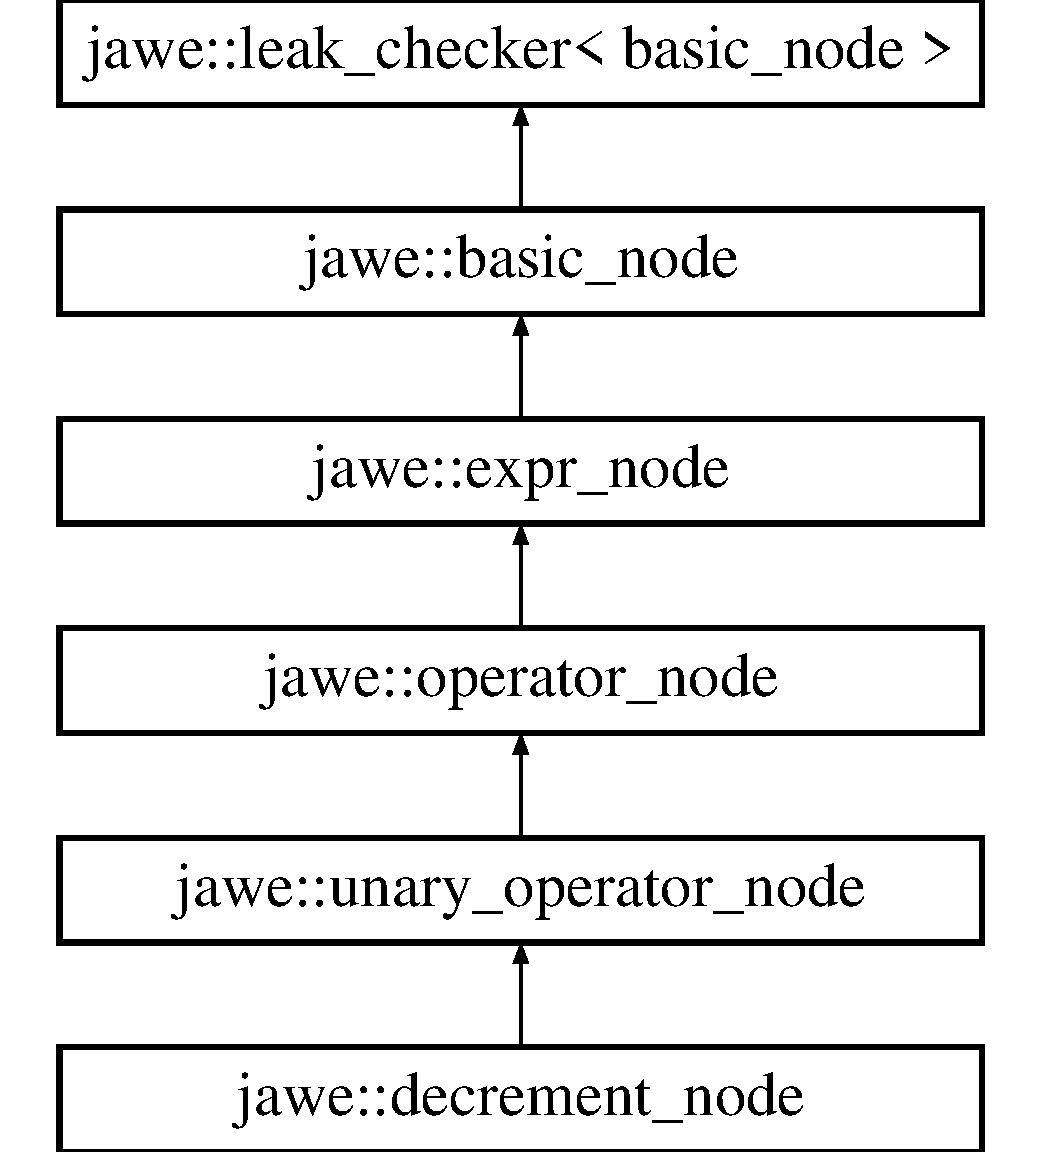
\includegraphics[height=6.000000cm]{classjawe_1_1decrement__node}
\end{center}
\end{figure}
\subsection*{Public Member Functions}
\begin{DoxyCompactItemize}
\item 
\hyperlink{classjawe_1_1decrement__node_aa1b25e1059bf8dc485bccd5a029dbea3}{decrement\+\_\+node} (const \hyperlink{namespacejawe_a3f307481d921b6cbb50cc8511fc2b544}{shared\+\_\+node} \&)
\end{DoxyCompactItemize}
\subsection*{Additional Inherited Members}


\subsection{Constructor \& Destructor Documentation}
\mbox{\Hypertarget{classjawe_1_1decrement__node_aa1b25e1059bf8dc485bccd5a029dbea3}\label{classjawe_1_1decrement__node_aa1b25e1059bf8dc485bccd5a029dbea3}} 
\index{jawe\+::decrement\+\_\+node@{jawe\+::decrement\+\_\+node}!decrement\+\_\+node@{decrement\+\_\+node}}
\index{decrement\+\_\+node@{decrement\+\_\+node}!jawe\+::decrement\+\_\+node@{jawe\+::decrement\+\_\+node}}
\subsubsection{\texorpdfstring{decrement\+\_\+node()}{decrement\_node()}}
{\footnotesize\ttfamily decrement\+\_\+node\+::decrement\+\_\+node (\begin{DoxyParamCaption}\item[{const \hyperlink{namespacejawe_a3f307481d921b6cbb50cc8511fc2b544}{shared\+\_\+node} \&}]{operand }\end{DoxyParamCaption})}



The documentation for this class was generated from the following files\+:\begin{DoxyCompactItemize}
\item 
include/syntax/operators/\hyperlink{decrement__node_8hpp}{decrement\+\_\+node.\+hpp}\item 
src/syntax/operators/\hyperlink{decrement__node_8cpp}{decrement\+\_\+node.\+cpp}\end{DoxyCompactItemize}

\hypertarget{classjawe_1_1default__node}{}\section{jawe\+:\+:default\+\_\+node Class Reference}
\label{classjawe_1_1default__node}\index{jawe\+::default\+\_\+node@{jawe\+::default\+\_\+node}}


{\ttfamily \#include $<$default\+\_\+node.\+hpp$>$}

Inheritance diagram for jawe\+:\+:default\+\_\+node\+:\begin{figure}[H]
\begin{center}
\leavevmode
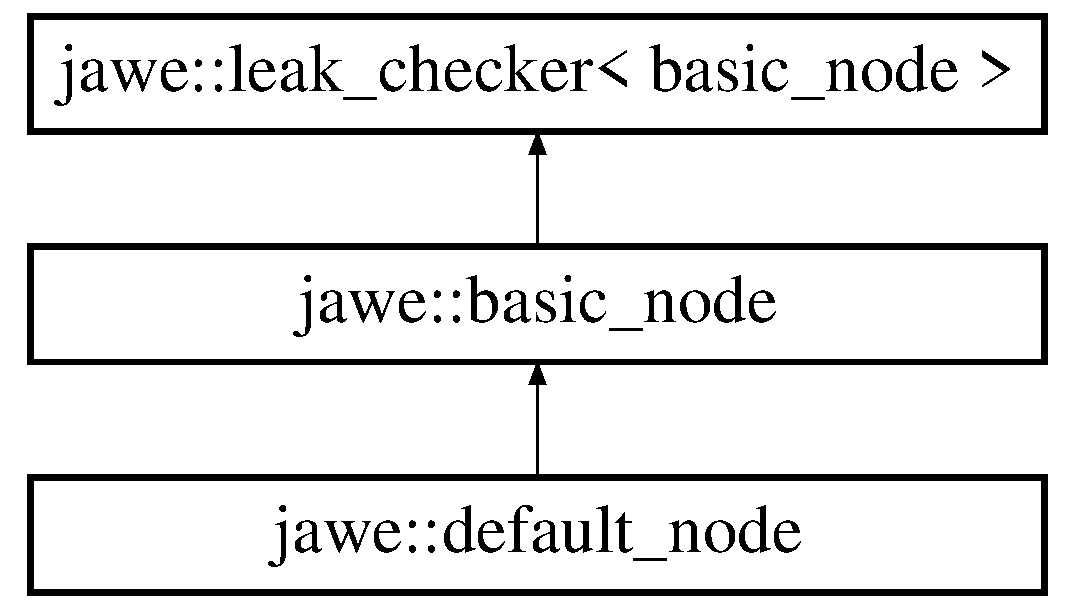
\includegraphics[height=3.000000cm]{classjawe_1_1default__node}
\end{center}
\end{figure}
\subsection*{Public Member Functions}
\begin{DoxyCompactItemize}
\item 
\hyperlink{classjawe_1_1default__node_a7c1eb033a8801fd4f2d7c65733c8dfea}{default\+\_\+node} (const \hyperlink{namespacejawe_a3f307481d921b6cbb50cc8511fc2b544}{shared\+\_\+node} \&)
\item 
\hyperlink{namespacejawe_a3f307481d921b6cbb50cc8511fc2b544}{shared\+\_\+node} \hyperlink{classjawe_1_1default__node_a9ea25fb0259faec5fd9b7b89711a61da}{get\+\_\+body} () const
\end{DoxyCompactItemize}
\subsection*{Private Attributes}
\begin{DoxyCompactItemize}
\item 
\hyperlink{namespacejawe_a3f307481d921b6cbb50cc8511fc2b544}{shared\+\_\+node} \hyperlink{classjawe_1_1default__node_a425524b6bbd0d56f7c3b07b194e227d2}{m\+\_\+command}
\end{DoxyCompactItemize}
\subsection*{Additional Inherited Members}


\subsection{Constructor \& Destructor Documentation}
\mbox{\Hypertarget{classjawe_1_1default__node_a7c1eb033a8801fd4f2d7c65733c8dfea}\label{classjawe_1_1default__node_a7c1eb033a8801fd4f2d7c65733c8dfea}} 
\index{jawe\+::default\+\_\+node@{jawe\+::default\+\_\+node}!default\+\_\+node@{default\+\_\+node}}
\index{default\+\_\+node@{default\+\_\+node}!jawe\+::default\+\_\+node@{jawe\+::default\+\_\+node}}
\subsubsection{\texorpdfstring{default\+\_\+node()}{default\_node()}}
{\footnotesize\ttfamily default\+\_\+node\+::default\+\_\+node (\begin{DoxyParamCaption}\item[{const \hyperlink{namespacejawe_a3f307481d921b6cbb50cc8511fc2b544}{shared\+\_\+node} \&}]{command }\end{DoxyParamCaption})}



\subsection{Member Function Documentation}
\mbox{\Hypertarget{classjawe_1_1default__node_a9ea25fb0259faec5fd9b7b89711a61da}\label{classjawe_1_1default__node_a9ea25fb0259faec5fd9b7b89711a61da}} 
\index{jawe\+::default\+\_\+node@{jawe\+::default\+\_\+node}!get\+\_\+body@{get\+\_\+body}}
\index{get\+\_\+body@{get\+\_\+body}!jawe\+::default\+\_\+node@{jawe\+::default\+\_\+node}}
\subsubsection{\texorpdfstring{get\+\_\+body()}{get\_body()}}
{\footnotesize\ttfamily \hyperlink{namespacejawe_a3f307481d921b6cbb50cc8511fc2b544}{shared\+\_\+node} default\+\_\+node\+::get\+\_\+body (\begin{DoxyParamCaption}{ }\end{DoxyParamCaption}) const}



\subsection{Member Data Documentation}
\mbox{\Hypertarget{classjawe_1_1default__node_a425524b6bbd0d56f7c3b07b194e227d2}\label{classjawe_1_1default__node_a425524b6bbd0d56f7c3b07b194e227d2}} 
\index{jawe\+::default\+\_\+node@{jawe\+::default\+\_\+node}!m\+\_\+command@{m\+\_\+command}}
\index{m\+\_\+command@{m\+\_\+command}!jawe\+::default\+\_\+node@{jawe\+::default\+\_\+node}}
\subsubsection{\texorpdfstring{m\+\_\+command}{m\_command}}
{\footnotesize\ttfamily \hyperlink{namespacejawe_a3f307481d921b6cbb50cc8511fc2b544}{shared\+\_\+node} jawe\+::default\+\_\+node\+::m\+\_\+command\hspace{0.3cm}{\ttfamily [private]}}



The documentation for this class was generated from the following files\+:\begin{DoxyCompactItemize}
\item 
include/syntax/control\+\_\+flow/\hyperlink{default__node_8hpp}{default\+\_\+node.\+hpp}\item 
src/syntax/control\+\_\+flow/\hyperlink{default__node_8cpp}{default\+\_\+node.\+cpp}\end{DoxyCompactItemize}

\hypertarget{classjawe_1_1delete__node}{}\section{jawe\+:\+:delete\+\_\+node Class Reference}
\label{classjawe_1_1delete__node}\index{jawe\+::delete\+\_\+node@{jawe\+::delete\+\_\+node}}


{\ttfamily \#include $<$delete\+\_\+node.\+hpp$>$}

Inheritance diagram for jawe\+:\+:delete\+\_\+node\+:\begin{figure}[H]
\begin{center}
\leavevmode
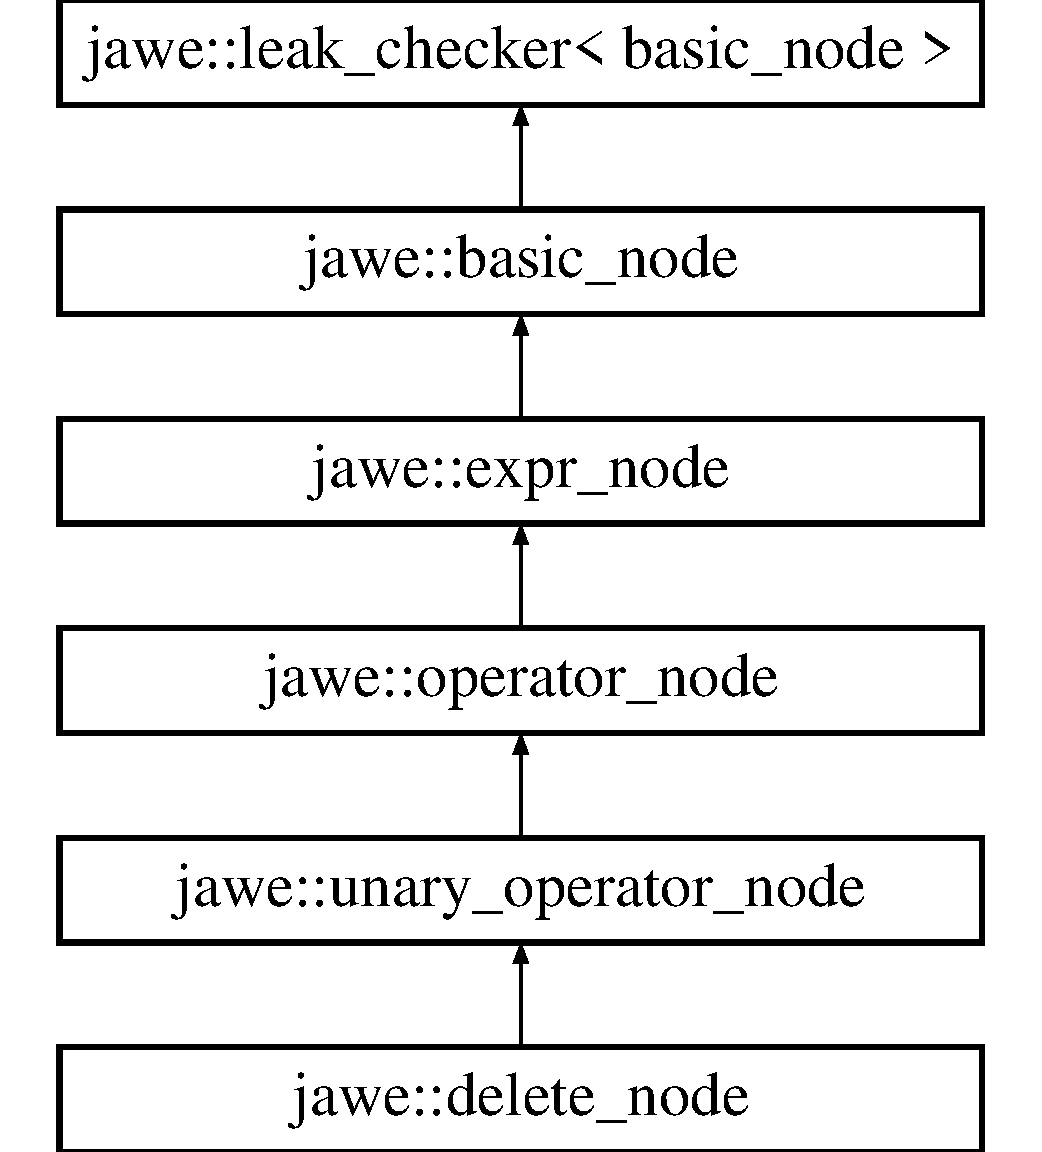
\includegraphics[height=6.000000cm]{classjawe_1_1delete__node}
\end{center}
\end{figure}
\subsection*{Public Member Functions}
\begin{DoxyCompactItemize}
\item 
\hyperlink{classjawe_1_1delete__node_a1b8bbb517992af65a52250cffa6602c5}{delete\+\_\+node} (const \hyperlink{namespacejawe_a3f307481d921b6cbb50cc8511fc2b544}{shared\+\_\+node} \&)
\end{DoxyCompactItemize}
\subsection*{Additional Inherited Members}


\subsection{Constructor \& Destructor Documentation}
\mbox{\Hypertarget{classjawe_1_1delete__node_a1b8bbb517992af65a52250cffa6602c5}\label{classjawe_1_1delete__node_a1b8bbb517992af65a52250cffa6602c5}} 
\index{jawe\+::delete\+\_\+node@{jawe\+::delete\+\_\+node}!delete\+\_\+node@{delete\+\_\+node}}
\index{delete\+\_\+node@{delete\+\_\+node}!jawe\+::delete\+\_\+node@{jawe\+::delete\+\_\+node}}
\subsubsection{\texorpdfstring{delete\+\_\+node()}{delete\_node()}}
{\footnotesize\ttfamily delete\+\_\+node\+::delete\+\_\+node (\begin{DoxyParamCaption}\item[{const \hyperlink{namespacejawe_a3f307481d921b6cbb50cc8511fc2b544}{shared\+\_\+node} \&}]{operand }\end{DoxyParamCaption})}



The documentation for this class was generated from the following files\+:\begin{DoxyCompactItemize}
\item 
include/syntax/operators/\hyperlink{delete__node_8hpp}{delete\+\_\+node.\+hpp}\item 
src/syntax/operators/\hyperlink{delete__node_8cpp}{delete\+\_\+node.\+cpp}\end{DoxyCompactItemize}

\hypertarget{structjawe_1_1deleter}{}\section{jawe\+:\+:deleter Struct Reference}
\label{structjawe_1_1deleter}\index{jawe\+::deleter@{jawe\+::deleter}}


{\ttfamily \#include $<$shared\+\_\+node.\+hpp$>$}

\subsection*{Public Member Functions}
\begin{DoxyCompactItemize}
\item 
void \hyperlink{structjawe_1_1deleter_ae05c400e87fe22be199bc4ed2d38a882}{operator()} (\hyperlink{namespacejawe_aca98f97d61e437678e7478e2d8aaf41f}{node\+\_\+variant} $\ast$)
\end{DoxyCompactItemize}


\subsection{Member Function Documentation}
\mbox{\Hypertarget{structjawe_1_1deleter_ae05c400e87fe22be199bc4ed2d38a882}\label{structjawe_1_1deleter_ae05c400e87fe22be199bc4ed2d38a882}} 
\index{jawe\+::deleter@{jawe\+::deleter}!operator()@{operator()}}
\index{operator()@{operator()}!jawe\+::deleter@{jawe\+::deleter}}
\subsubsection{\texorpdfstring{operator()()}{operator()()}}
{\footnotesize\ttfamily void deleter\+::operator() (\begin{DoxyParamCaption}\item[{\hyperlink{namespacejawe_aca98f97d61e437678e7478e2d8aaf41f}{node\+\_\+variant} $\ast$}]{node }\end{DoxyParamCaption})}



The documentation for this struct was generated from the following files\+:\begin{DoxyCompactItemize}
\item 
include/syntax/abstract/\hyperlink{shared__node_8hpp}{shared\+\_\+node.\+hpp}\item 
src/syntax/abstract/\hyperlink{shared__node_8cpp}{shared\+\_\+node.\+cpp}\end{DoxyCompactItemize}

\hypertarget{classjawe_1_1divide__node}{}\section{jawe\+:\+:divide\+\_\+node Class Reference}
\label{classjawe_1_1divide__node}\index{jawe\+::divide\+\_\+node@{jawe\+::divide\+\_\+node}}


{\ttfamily \#include $<$divide\+\_\+node.\+hpp$>$}

Inheritance diagram for jawe\+:\+:divide\+\_\+node\+:\begin{figure}[H]
\begin{center}
\leavevmode
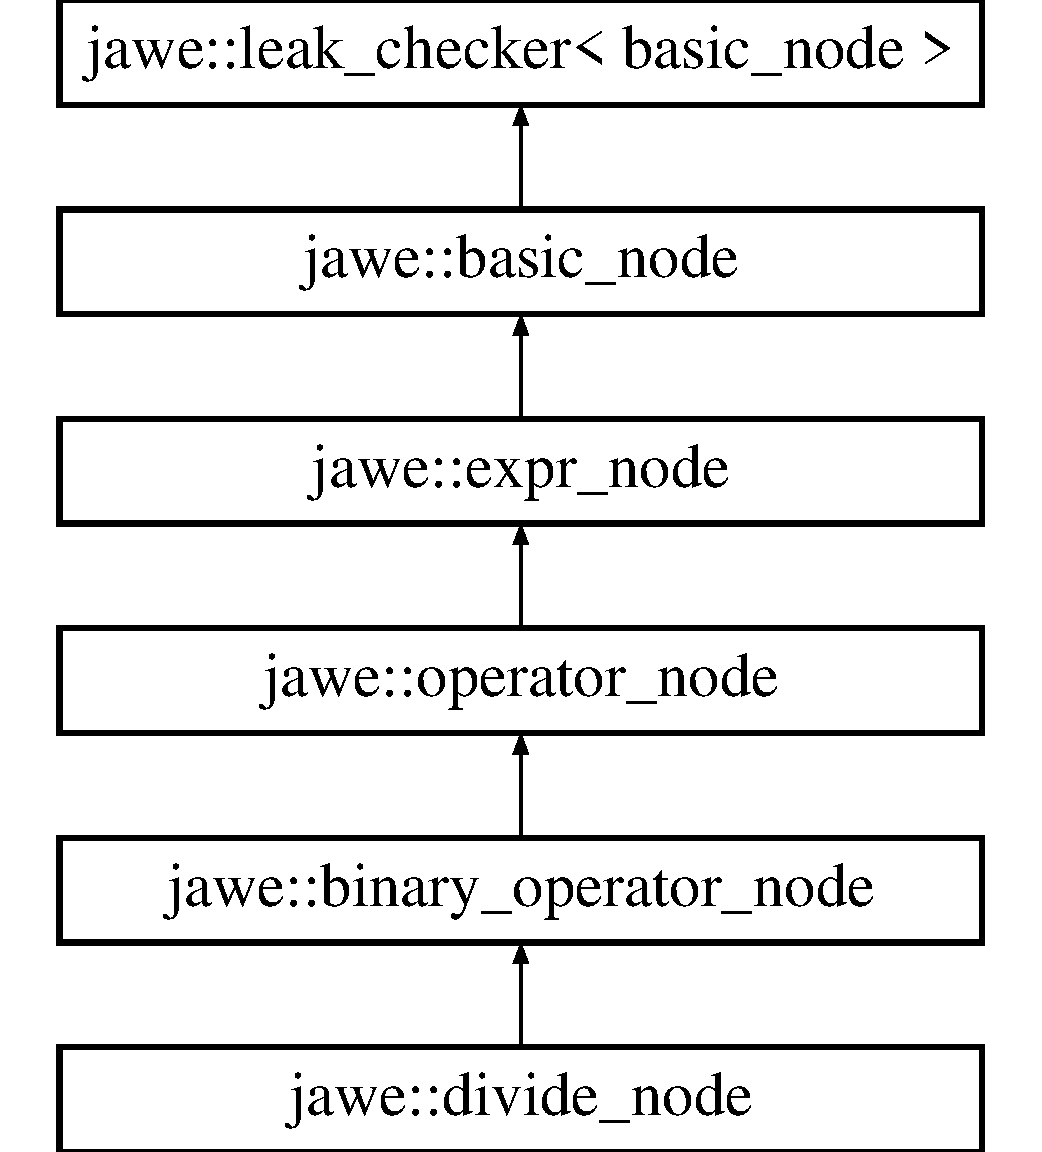
\includegraphics[height=6.000000cm]{classjawe_1_1divide__node}
\end{center}
\end{figure}
\subsection*{Public Member Functions}
\begin{DoxyCompactItemize}
\item 
\hyperlink{classjawe_1_1divide__node_a91819747503211c892a0055a5284e241}{divide\+\_\+node} (const \hyperlink{namespacejawe_a3f307481d921b6cbb50cc8511fc2b544}{shared\+\_\+node} \&, const \hyperlink{namespacejawe_a3f307481d921b6cbb50cc8511fc2b544}{shared\+\_\+node} \&)
\end{DoxyCompactItemize}
\subsection*{Additional Inherited Members}


\subsection{Constructor \& Destructor Documentation}
\mbox{\Hypertarget{classjawe_1_1divide__node_a91819747503211c892a0055a5284e241}\label{classjawe_1_1divide__node_a91819747503211c892a0055a5284e241}} 
\index{jawe\+::divide\+\_\+node@{jawe\+::divide\+\_\+node}!divide\+\_\+node@{divide\+\_\+node}}
\index{divide\+\_\+node@{divide\+\_\+node}!jawe\+::divide\+\_\+node@{jawe\+::divide\+\_\+node}}
\subsubsection{\texorpdfstring{divide\+\_\+node()}{divide\_node()}}
{\footnotesize\ttfamily divide\+\_\+node\+::divide\+\_\+node (\begin{DoxyParamCaption}\item[{const \hyperlink{namespacejawe_a3f307481d921b6cbb50cc8511fc2b544}{shared\+\_\+node} \&}]{left,  }\item[{const \hyperlink{namespacejawe_a3f307481d921b6cbb50cc8511fc2b544}{shared\+\_\+node} \&}]{right }\end{DoxyParamCaption})}



The documentation for this class was generated from the following files\+:\begin{DoxyCompactItemize}
\item 
include/syntax/operators/\hyperlink{divide__node_8hpp}{divide\+\_\+node.\+hpp}\item 
src/syntax/operators/\hyperlink{divide__node_8cpp}{divide\+\_\+node.\+cpp}\end{DoxyCompactItemize}

\hypertarget{classjawe_1_1do__while__node}{}\section{jawe\+:\+:do\+\_\+while\+\_\+node Class Reference}
\label{classjawe_1_1do__while__node}\index{jawe\+::do\+\_\+while\+\_\+node@{jawe\+::do\+\_\+while\+\_\+node}}


{\ttfamily \#include $<$do\+\_\+while\+\_\+node.\+hpp$>$}

Inheritance diagram for jawe\+:\+:do\+\_\+while\+\_\+node\+:\begin{figure}[H]
\begin{center}
\leavevmode
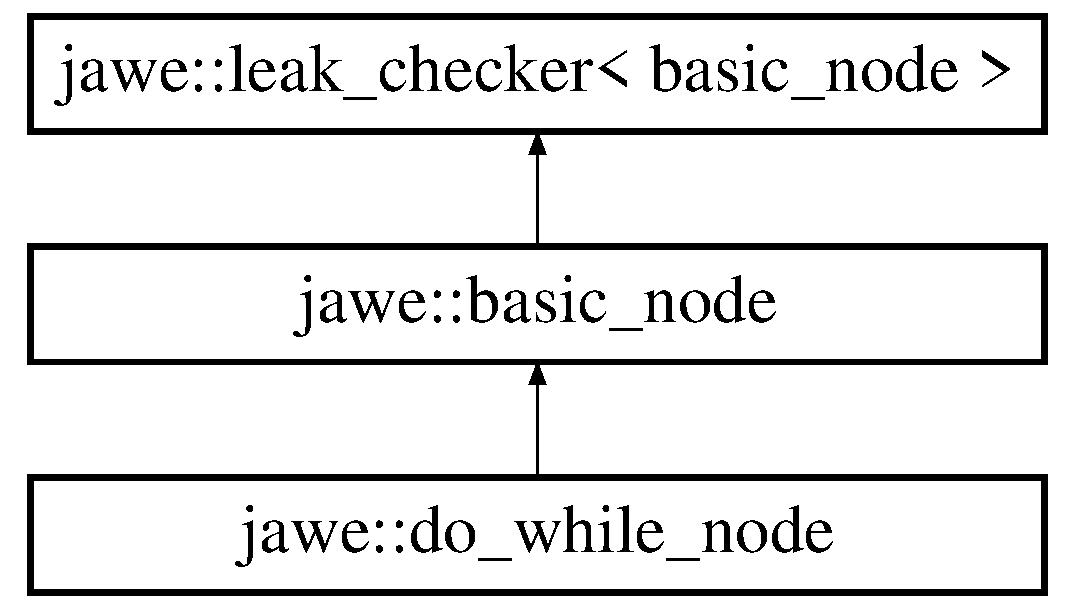
\includegraphics[height=3.000000cm]{classjawe_1_1do__while__node}
\end{center}
\end{figure}
\subsection*{Public Member Functions}
\begin{DoxyCompactItemize}
\item 
\hyperlink{classjawe_1_1do__while__node_a9d18fb637c871e855cb853ee3e3e0bf3}{do\+\_\+while\+\_\+node} (const \hyperlink{namespacejawe_a3f307481d921b6cbb50cc8511fc2b544}{shared\+\_\+node} \&, const \hyperlink{namespacejawe_a3f307481d921b6cbb50cc8511fc2b544}{shared\+\_\+node} \&)
\item 
\hyperlink{namespacejawe_a3f307481d921b6cbb50cc8511fc2b544}{shared\+\_\+node} \hyperlink{classjawe_1_1do__while__node_a4b9b594ac5555ef726b9973996658392}{get\+\_\+expr} () const
\item 
\hyperlink{namespacejawe_a3f307481d921b6cbb50cc8511fc2b544}{shared\+\_\+node} \hyperlink{classjawe_1_1do__while__node_aea8cf6c53e681bc884eb785cdf52e9f5}{get\+\_\+body} () const
\end{DoxyCompactItemize}
\subsection*{Private Attributes}
\begin{DoxyCompactItemize}
\item 
\hyperlink{namespacejawe_a3f307481d921b6cbb50cc8511fc2b544}{shared\+\_\+node} \hyperlink{classjawe_1_1do__while__node_a35de6d1c09f9bc8bfbf74c9e617111e3}{m\+\_\+body}
\item 
\hyperlink{namespacejawe_a3f307481d921b6cbb50cc8511fc2b544}{shared\+\_\+node} \hyperlink{classjawe_1_1do__while__node_a9f0777b8820faf8513b523a00e6cbdd7}{m\+\_\+cond}
\end{DoxyCompactItemize}
\subsection*{Additional Inherited Members}


\subsection{Constructor \& Destructor Documentation}
\mbox{\Hypertarget{classjawe_1_1do__while__node_a9d18fb637c871e855cb853ee3e3e0bf3}\label{classjawe_1_1do__while__node_a9d18fb637c871e855cb853ee3e3e0bf3}} 
\index{jawe\+::do\+\_\+while\+\_\+node@{jawe\+::do\+\_\+while\+\_\+node}!do\+\_\+while\+\_\+node@{do\+\_\+while\+\_\+node}}
\index{do\+\_\+while\+\_\+node@{do\+\_\+while\+\_\+node}!jawe\+::do\+\_\+while\+\_\+node@{jawe\+::do\+\_\+while\+\_\+node}}
\subsubsection{\texorpdfstring{do\+\_\+while\+\_\+node()}{do\_while\_node()}}
{\footnotesize\ttfamily do\+\_\+while\+\_\+node\+::do\+\_\+while\+\_\+node (\begin{DoxyParamCaption}\item[{const \hyperlink{namespacejawe_a3f307481d921b6cbb50cc8511fc2b544}{shared\+\_\+node} \&}]{body,  }\item[{const \hyperlink{namespacejawe_a3f307481d921b6cbb50cc8511fc2b544}{shared\+\_\+node} \&}]{cond }\end{DoxyParamCaption})}



\subsection{Member Function Documentation}
\mbox{\Hypertarget{classjawe_1_1do__while__node_aea8cf6c53e681bc884eb785cdf52e9f5}\label{classjawe_1_1do__while__node_aea8cf6c53e681bc884eb785cdf52e9f5}} 
\index{jawe\+::do\+\_\+while\+\_\+node@{jawe\+::do\+\_\+while\+\_\+node}!get\+\_\+body@{get\+\_\+body}}
\index{get\+\_\+body@{get\+\_\+body}!jawe\+::do\+\_\+while\+\_\+node@{jawe\+::do\+\_\+while\+\_\+node}}
\subsubsection{\texorpdfstring{get\+\_\+body()}{get\_body()}}
{\footnotesize\ttfamily \hyperlink{namespacejawe_a3f307481d921b6cbb50cc8511fc2b544}{shared\+\_\+node} do\+\_\+while\+\_\+node\+::get\+\_\+body (\begin{DoxyParamCaption}{ }\end{DoxyParamCaption}) const}

\mbox{\Hypertarget{classjawe_1_1do__while__node_a4b9b594ac5555ef726b9973996658392}\label{classjawe_1_1do__while__node_a4b9b594ac5555ef726b9973996658392}} 
\index{jawe\+::do\+\_\+while\+\_\+node@{jawe\+::do\+\_\+while\+\_\+node}!get\+\_\+expr@{get\+\_\+expr}}
\index{get\+\_\+expr@{get\+\_\+expr}!jawe\+::do\+\_\+while\+\_\+node@{jawe\+::do\+\_\+while\+\_\+node}}
\subsubsection{\texorpdfstring{get\+\_\+expr()}{get\_expr()}}
{\footnotesize\ttfamily \hyperlink{namespacejawe_a3f307481d921b6cbb50cc8511fc2b544}{shared\+\_\+node} do\+\_\+while\+\_\+node\+::get\+\_\+expr (\begin{DoxyParamCaption}{ }\end{DoxyParamCaption}) const}



\subsection{Member Data Documentation}
\mbox{\Hypertarget{classjawe_1_1do__while__node_a35de6d1c09f9bc8bfbf74c9e617111e3}\label{classjawe_1_1do__while__node_a35de6d1c09f9bc8bfbf74c9e617111e3}} 
\index{jawe\+::do\+\_\+while\+\_\+node@{jawe\+::do\+\_\+while\+\_\+node}!m\+\_\+body@{m\+\_\+body}}
\index{m\+\_\+body@{m\+\_\+body}!jawe\+::do\+\_\+while\+\_\+node@{jawe\+::do\+\_\+while\+\_\+node}}
\subsubsection{\texorpdfstring{m\+\_\+body}{m\_body}}
{\footnotesize\ttfamily \hyperlink{namespacejawe_a3f307481d921b6cbb50cc8511fc2b544}{shared\+\_\+node} jawe\+::do\+\_\+while\+\_\+node\+::m\+\_\+body\hspace{0.3cm}{\ttfamily [private]}}

\mbox{\Hypertarget{classjawe_1_1do__while__node_a9f0777b8820faf8513b523a00e6cbdd7}\label{classjawe_1_1do__while__node_a9f0777b8820faf8513b523a00e6cbdd7}} 
\index{jawe\+::do\+\_\+while\+\_\+node@{jawe\+::do\+\_\+while\+\_\+node}!m\+\_\+cond@{m\+\_\+cond}}
\index{m\+\_\+cond@{m\+\_\+cond}!jawe\+::do\+\_\+while\+\_\+node@{jawe\+::do\+\_\+while\+\_\+node}}
\subsubsection{\texorpdfstring{m\+\_\+cond}{m\_cond}}
{\footnotesize\ttfamily \hyperlink{namespacejawe_a3f307481d921b6cbb50cc8511fc2b544}{shared\+\_\+node} jawe\+::do\+\_\+while\+\_\+node\+::m\+\_\+cond\hspace{0.3cm}{\ttfamily [private]}}



The documentation for this class was generated from the following files\+:\begin{DoxyCompactItemize}
\item 
include/syntax/control\+\_\+flow/\hyperlink{do__while__node_8hpp}{do\+\_\+while\+\_\+node.\+hpp}\item 
src/syntax/control\+\_\+flow/\hyperlink{do__while__node_8cpp}{do\+\_\+while\+\_\+node.\+cpp}\end{DoxyCompactItemize}

\hypertarget{classjawe_1_1dot__access__node}{}\section{jawe\+:\+:dot\+\_\+access\+\_\+node Class Reference}
\label{classjawe_1_1dot__access__node}\index{jawe\+::dot\+\_\+access\+\_\+node@{jawe\+::dot\+\_\+access\+\_\+node}}


{\ttfamily \#include $<$dot\+\_\+access\+\_\+node.\+hpp$>$}

Inheritance diagram for jawe\+:\+:dot\+\_\+access\+\_\+node\+:\begin{figure}[H]
\begin{center}
\leavevmode
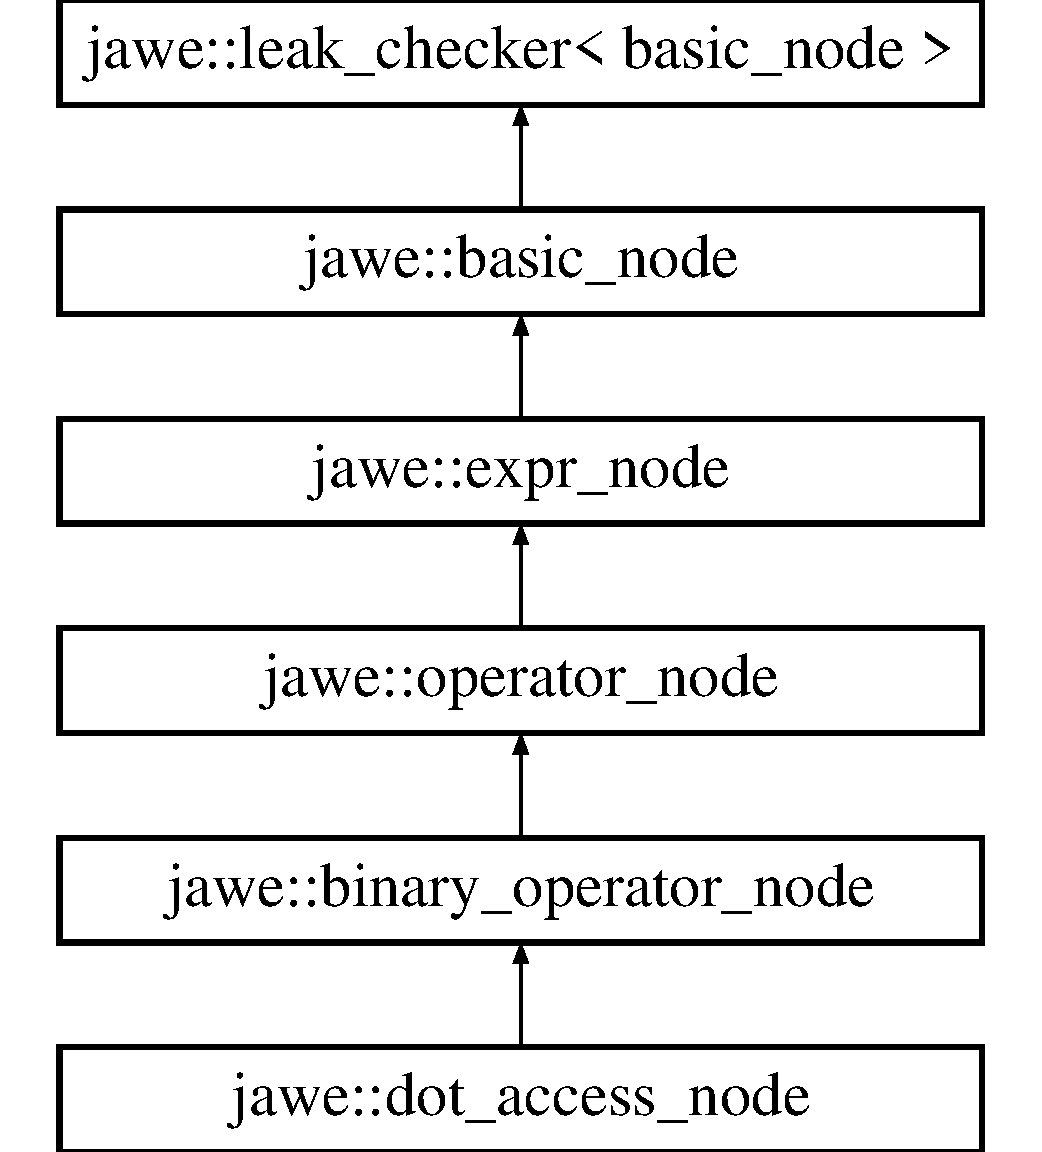
\includegraphics[height=6.000000cm]{classjawe_1_1dot__access__node}
\end{center}
\end{figure}
\subsection*{Public Member Functions}
\begin{DoxyCompactItemize}
\item 
\hyperlink{classjawe_1_1dot__access__node_a37f230071af08407536141fa8dc65f59}{dot\+\_\+access\+\_\+node} (const \hyperlink{namespacejawe_a3f307481d921b6cbb50cc8511fc2b544}{shared\+\_\+node} \&, const \hyperlink{namespacejawe_a3f307481d921b6cbb50cc8511fc2b544}{shared\+\_\+node} \&)
\end{DoxyCompactItemize}
\subsection*{Additional Inherited Members}


\subsection{Constructor \& Destructor Documentation}
\mbox{\Hypertarget{classjawe_1_1dot__access__node_a37f230071af08407536141fa8dc65f59}\label{classjawe_1_1dot__access__node_a37f230071af08407536141fa8dc65f59}} 
\index{jawe\+::dot\+\_\+access\+\_\+node@{jawe\+::dot\+\_\+access\+\_\+node}!dot\+\_\+access\+\_\+node@{dot\+\_\+access\+\_\+node}}
\index{dot\+\_\+access\+\_\+node@{dot\+\_\+access\+\_\+node}!jawe\+::dot\+\_\+access\+\_\+node@{jawe\+::dot\+\_\+access\+\_\+node}}
\subsubsection{\texorpdfstring{dot\+\_\+access\+\_\+node()}{dot\_access\_node()}}
{\footnotesize\ttfamily dot\+\_\+access\+\_\+node\+::dot\+\_\+access\+\_\+node (\begin{DoxyParamCaption}\item[{const \hyperlink{namespacejawe_a3f307481d921b6cbb50cc8511fc2b544}{shared\+\_\+node} \&}]{left,  }\item[{const \hyperlink{namespacejawe_a3f307481d921b6cbb50cc8511fc2b544}{shared\+\_\+node} \&}]{right }\end{DoxyParamCaption})}



The documentation for this class was generated from the following files\+:\begin{DoxyCompactItemize}
\item 
include/syntax/operators/\hyperlink{dot__access__node_8hpp}{dot\+\_\+access\+\_\+node.\+hpp}\item 
src/syntax/operators/\hyperlink{dot__access__node_8cpp}{dot\+\_\+access\+\_\+node.\+cpp}\end{DoxyCompactItemize}

\hypertarget{classjawe_1_1utils_1_1empty}{}\section{jawe\+:\+:utils\+:\+:empty Class Reference}
\label{classjawe_1_1utils_1_1empty}\index{jawe\+::utils\+::empty@{jawe\+::utils\+::empty}}


Empty class used for specialization of non-\/container class template.  




{\ttfamily \#include $<$scope.\+hpp$>$}



\subsection{Detailed Description}
Empty class used for specialization of non-\/container class template. 

The documentation for this class was generated from the following file\+:\begin{DoxyCompactItemize}
\item 
include/utils/\hyperlink{scope_8hpp}{scope.\+hpp}\end{DoxyCompactItemize}

\hypertarget{classjawe_1_1empty__node}{}\section{jawe\+:\+:empty\+\_\+node Class Reference}
\label{classjawe_1_1empty__node}\index{jawe\+::empty\+\_\+node@{jawe\+::empty\+\_\+node}}


{\ttfamily \#include $<$empty\+\_\+node.\+hpp$>$}

Inheritance diagram for jawe\+:\+:empty\+\_\+node\+:\begin{figure}[H]
\begin{center}
\leavevmode
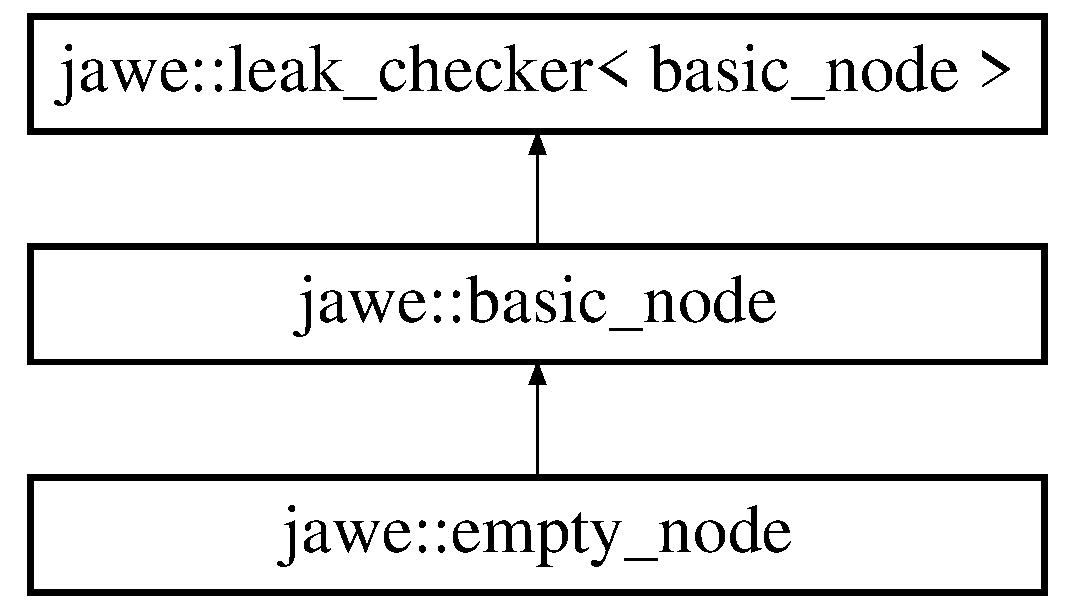
\includegraphics[height=3.000000cm]{classjawe_1_1empty__node}
\end{center}
\end{figure}
\subsection*{Public Member Functions}
\begin{DoxyCompactItemize}
\item 
\hyperlink{classjawe_1_1empty__node_adbc815c4256a01b49cbff01f9dc55431}{empty\+\_\+node} ()
\end{DoxyCompactItemize}
\subsection*{Additional Inherited Members}


\subsection{Constructor \& Destructor Documentation}
\mbox{\Hypertarget{classjawe_1_1empty__node_adbc815c4256a01b49cbff01f9dc55431}\label{classjawe_1_1empty__node_adbc815c4256a01b49cbff01f9dc55431}} 
\index{jawe\+::empty\+\_\+node@{jawe\+::empty\+\_\+node}!empty\+\_\+node@{empty\+\_\+node}}
\index{empty\+\_\+node@{empty\+\_\+node}!jawe\+::empty\+\_\+node@{jawe\+::empty\+\_\+node}}
\subsubsection{\texorpdfstring{empty\+\_\+node()}{empty\_node()}}
{\footnotesize\ttfamily empty\+\_\+node\+::empty\+\_\+node (\begin{DoxyParamCaption}{ }\end{DoxyParamCaption})}



The documentation for this class was generated from the following files\+:\begin{DoxyCompactItemize}
\item 
include/syntax/control\+\_\+flow/\hyperlink{empty__node_8hpp}{empty\+\_\+node.\+hpp}\item 
src/syntax/control\+\_\+flow/\hyperlink{empty__node_8cpp}{empty\+\_\+node.\+cpp}\end{DoxyCompactItemize}

\hypertarget{classjawe_1_1empty__remover}{}\section{jawe\+:\+:empty\+\_\+remover Class Reference}
\label{classjawe_1_1empty__remover}\index{jawe\+::empty\+\_\+remover@{jawe\+::empty\+\_\+remover}}


{\ttfamily \#include $<$empty\+\_\+remover.\+hpp$>$}

Inheritance diagram for jawe\+:\+:empty\+\_\+remover\+:\begin{figure}[H]
\begin{center}
\leavevmode
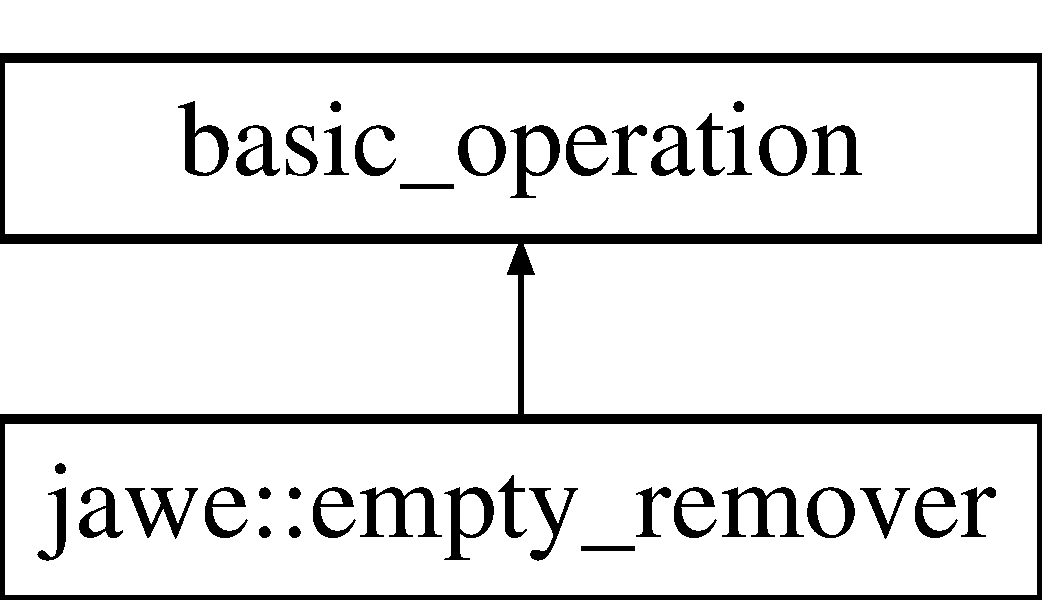
\includegraphics[height=2.000000cm]{classjawe_1_1empty__remover}
\end{center}
\end{figure}
\subsection*{Public Member Functions}
\begin{DoxyCompactItemize}
\item 
void \hyperlink{classjawe_1_1empty__remover_af369f9e6202276fc09d8b21271916c7e}{run} () const
\end{DoxyCompactItemize}
\subsection*{Private Member Functions}
\begin{DoxyCompactItemize}
\item 
void \hyperlink{classjawe_1_1empty__remover_aa2e19828a73d38052e21dc5a58826916}{remove} (const \hyperlink{namespacejawe_a3f307481d921b6cbb50cc8511fc2b544}{shared\+\_\+node} \&, const \hyperlink{namespacejawe_a3f307481d921b6cbb50cc8511fc2b544}{shared\+\_\+node} \&) const
\item 
void \hyperlink{classjawe_1_1empty__remover_a4e97d479ce5a67b38fe904b7ab017f94}{remove\+\_\+impl} (const \hyperlink{namespacejawe_a3f307481d921b6cbb50cc8511fc2b544}{shared\+\_\+node} \&, const \hyperlink{namespacejawe_a3f307481d921b6cbb50cc8511fc2b544}{shared\+\_\+node} \&) const
\end{DoxyCompactItemize}


\subsection{Member Function Documentation}
\mbox{\Hypertarget{classjawe_1_1empty__remover_aa2e19828a73d38052e21dc5a58826916}\label{classjawe_1_1empty__remover_aa2e19828a73d38052e21dc5a58826916}} 
\index{jawe\+::empty\+\_\+remover@{jawe\+::empty\+\_\+remover}!remove@{remove}}
\index{remove@{remove}!jawe\+::empty\+\_\+remover@{jawe\+::empty\+\_\+remover}}
\subsubsection{\texorpdfstring{remove()}{remove()}}
{\footnotesize\ttfamily void empty\+\_\+remover\+::remove (\begin{DoxyParamCaption}\item[{const \hyperlink{namespacejawe_a3f307481d921b6cbb50cc8511fc2b544}{shared\+\_\+node} \&}]{root,  }\item[{const \hyperlink{namespacejawe_a3f307481d921b6cbb50cc8511fc2b544}{shared\+\_\+node} \&}]{parent }\end{DoxyParamCaption}) const\hspace{0.3cm}{\ttfamily [private]}}

\mbox{\Hypertarget{classjawe_1_1empty__remover_a4e97d479ce5a67b38fe904b7ab017f94}\label{classjawe_1_1empty__remover_a4e97d479ce5a67b38fe904b7ab017f94}} 
\index{jawe\+::empty\+\_\+remover@{jawe\+::empty\+\_\+remover}!remove\+\_\+impl@{remove\+\_\+impl}}
\index{remove\+\_\+impl@{remove\+\_\+impl}!jawe\+::empty\+\_\+remover@{jawe\+::empty\+\_\+remover}}
\subsubsection{\texorpdfstring{remove\+\_\+impl()}{remove\_impl()}}
{\footnotesize\ttfamily void empty\+\_\+remover\+::remove\+\_\+impl (\begin{DoxyParamCaption}\item[{const \hyperlink{namespacejawe_a3f307481d921b6cbb50cc8511fc2b544}{shared\+\_\+node} \&}]{child,  }\item[{const \hyperlink{namespacejawe_a3f307481d921b6cbb50cc8511fc2b544}{shared\+\_\+node} \&}]{parent }\end{DoxyParamCaption}) const\hspace{0.3cm}{\ttfamily [private]}}

\mbox{\Hypertarget{classjawe_1_1empty__remover_af369f9e6202276fc09d8b21271916c7e}\label{classjawe_1_1empty__remover_af369f9e6202276fc09d8b21271916c7e}} 
\index{jawe\+::empty\+\_\+remover@{jawe\+::empty\+\_\+remover}!run@{run}}
\index{run@{run}!jawe\+::empty\+\_\+remover@{jawe\+::empty\+\_\+remover}}
\subsubsection{\texorpdfstring{run()}{run()}}
{\footnotesize\ttfamily void empty\+\_\+remover\+::run (\begin{DoxyParamCaption}{ }\end{DoxyParamCaption}) const}



The documentation for this class was generated from the following files\+:\begin{DoxyCompactItemize}
\item 
include/operations/\hyperlink{empty__remover_8hpp}{empty\+\_\+remover.\+hpp}\item 
src/operations/\hyperlink{empty__remover_8cpp}{empty\+\_\+remover.\+cpp}\end{DoxyCompactItemize}

\hypertarget{classjawe_1_1equals__node}{}\section{jawe\+:\+:equals\+\_\+node Class Reference}
\label{classjawe_1_1equals__node}\index{jawe\+::equals\+\_\+node@{jawe\+::equals\+\_\+node}}


{\ttfamily \#include $<$equals\+\_\+node.\+hpp$>$}

Inheritance diagram for jawe\+:\+:equals\+\_\+node\+:\begin{figure}[H]
\begin{center}
\leavevmode
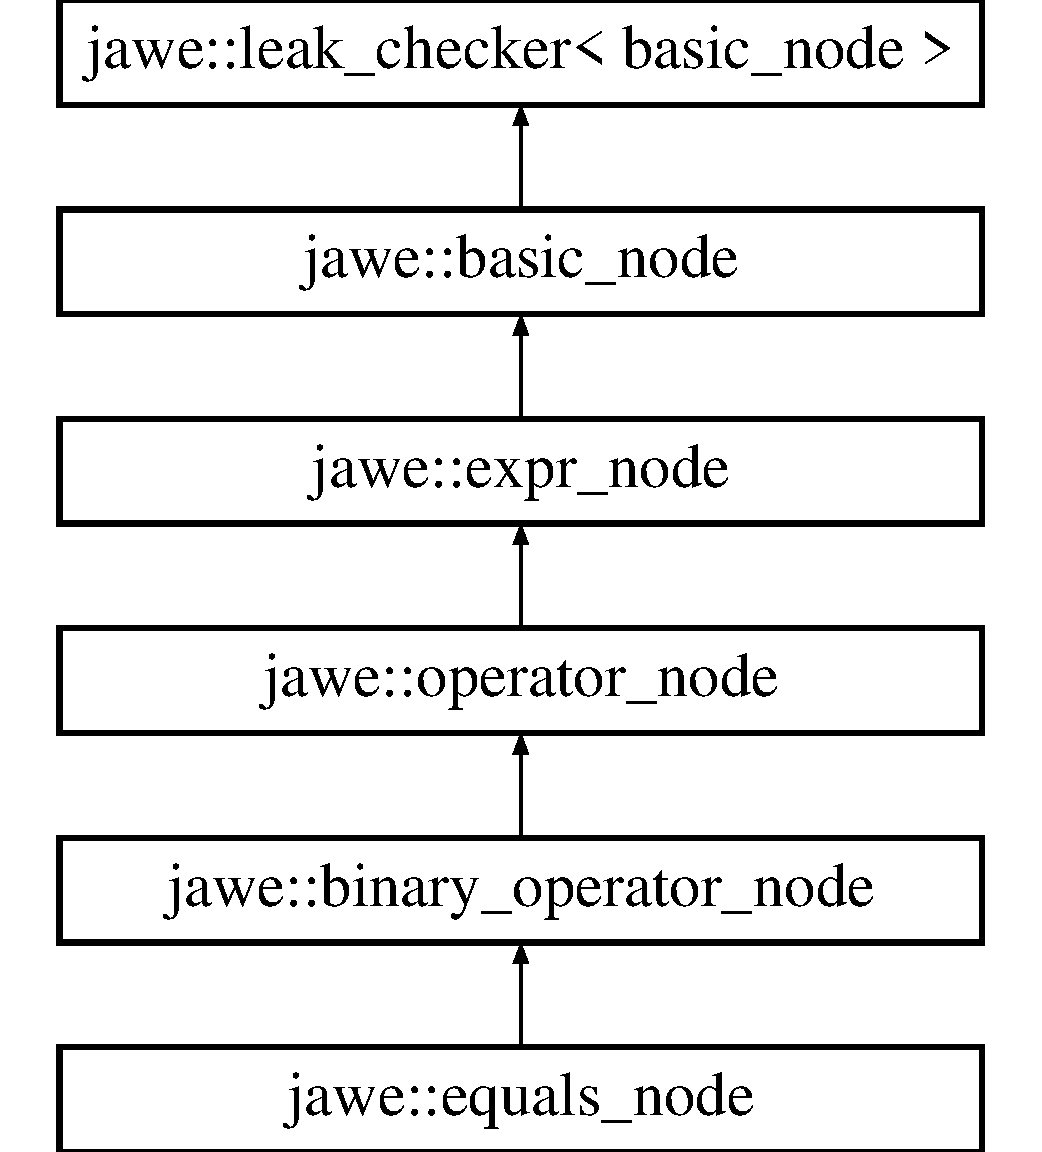
\includegraphics[height=6.000000cm]{classjawe_1_1equals__node}
\end{center}
\end{figure}
\subsection*{Public Member Functions}
\begin{DoxyCompactItemize}
\item 
\hyperlink{classjawe_1_1equals__node_a991c13e39ea1bdf2553fb26d0bf8fa3b}{equals\+\_\+node} (const \hyperlink{namespacejawe_a3f307481d921b6cbb50cc8511fc2b544}{shared\+\_\+node} \&, const \hyperlink{namespacejawe_a3f307481d921b6cbb50cc8511fc2b544}{shared\+\_\+node} \&)
\end{DoxyCompactItemize}
\subsection*{Additional Inherited Members}


\subsection{Constructor \& Destructor Documentation}
\mbox{\Hypertarget{classjawe_1_1equals__node_a991c13e39ea1bdf2553fb26d0bf8fa3b}\label{classjawe_1_1equals__node_a991c13e39ea1bdf2553fb26d0bf8fa3b}} 
\index{jawe\+::equals\+\_\+node@{jawe\+::equals\+\_\+node}!equals\+\_\+node@{equals\+\_\+node}}
\index{equals\+\_\+node@{equals\+\_\+node}!jawe\+::equals\+\_\+node@{jawe\+::equals\+\_\+node}}
\subsubsection{\texorpdfstring{equals\+\_\+node()}{equals\_node()}}
{\footnotesize\ttfamily equals\+\_\+node\+::equals\+\_\+node (\begin{DoxyParamCaption}\item[{const \hyperlink{namespacejawe_a3f307481d921b6cbb50cc8511fc2b544}{shared\+\_\+node} \&}]{left,  }\item[{const \hyperlink{namespacejawe_a3f307481d921b6cbb50cc8511fc2b544}{shared\+\_\+node} \&}]{right }\end{DoxyParamCaption})}



The documentation for this class was generated from the following files\+:\begin{DoxyCompactItemize}
\item 
include/syntax/operators/\hyperlink{equals__node_8hpp}{equals\+\_\+node.\+hpp}\item 
src/syntax/operators/\hyperlink{equals__node_8cpp}{equals\+\_\+node.\+cpp}\end{DoxyCompactItemize}

\hypertarget{classjawe_1_1error__reporter}{}\section{jawe\+:\+:error\+\_\+reporter Class Reference}
\label{classjawe_1_1error__reporter}\index{jawe\+::error\+\_\+reporter@{jawe\+::error\+\_\+reporter}}


Class used as main error reporting system throughout the project.  




{\ttfamily \#include $<$error\+\_\+reporter.\+hpp$>$}

\subsection*{Static Public Member Functions}
\begin{DoxyCompactItemize}
\item 
static void \hyperlink{classjawe_1_1error__reporter_acfa7b31326b9919ecdd1d1c13053c658}{error} (const std\+::string \&msg)
\item 
static void \hyperlink{classjawe_1_1error__reporter_a61739ea73525d07a47a1054ec3de88dc}{error} (const std\+::string \&msg, int row\+\_\+no, int col\+\_\+no)
\item 
static void \hyperlink{classjawe_1_1error__reporter_ad0ae5f6a65fb62897239a5efdf7d1d7b}{error} (const std\+::string \&msg, const \hyperlink{namespacejawe_a3f307481d921b6cbb50cc8511fc2b544}{shared\+\_\+node} \&node)
\end{DoxyCompactItemize}
\subsection*{Static Private Member Functions}
\begin{DoxyCompactItemize}
\item 
static void \hyperlink{classjawe_1_1error__reporter_afd5cdb8c419376a45200d2b93dddd20b}{print\+\_\+line} (const std\+::string \&msg, int row\+\_\+no, int col\+\_\+no)
\end{DoxyCompactItemize}


\subsection{Detailed Description}
Class used as main error reporting system throughout the project. 

This class is can be used in all phases of compilation (parser, semantic analyzer...). 

\subsection{Member Function Documentation}
\mbox{\Hypertarget{classjawe_1_1error__reporter_acfa7b31326b9919ecdd1d1c13053c658}\label{classjawe_1_1error__reporter_acfa7b31326b9919ecdd1d1c13053c658}} 
\index{jawe\+::error\+\_\+reporter@{jawe\+::error\+\_\+reporter}!error@{error}}
\index{error@{error}!jawe\+::error\+\_\+reporter@{jawe\+::error\+\_\+reporter}}
\subsubsection{\texorpdfstring{error()}{error()}\hspace{0.1cm}{\footnotesize\ttfamily [1/3]}}
{\footnotesize\ttfamily void error\+\_\+reporter\+::error (\begin{DoxyParamCaption}\item[{const std\+::string \&}]{msg }\end{DoxyParamCaption})\hspace{0.3cm}{\ttfamily [static]}}

Reports error message.

This function should be used only in parsing phase since it will gather location information from the reader (it\textquotesingle{}ll use lastly buffered state).


\begin{DoxyParams}{Parameters}
{\em msg} & message that is to be written to the user. \\
\hline
\end{DoxyParams}
\mbox{\Hypertarget{classjawe_1_1error__reporter_a61739ea73525d07a47a1054ec3de88dc}\label{classjawe_1_1error__reporter_a61739ea73525d07a47a1054ec3de88dc}} 
\index{jawe\+::error\+\_\+reporter@{jawe\+::error\+\_\+reporter}!error@{error}}
\index{error@{error}!jawe\+::error\+\_\+reporter@{jawe\+::error\+\_\+reporter}}
\subsubsection{\texorpdfstring{error()}{error()}\hspace{0.1cm}{\footnotesize\ttfamily [2/3]}}
{\footnotesize\ttfamily void error\+\_\+reporter\+::error (\begin{DoxyParamCaption}\item[{const std\+::string \&}]{msg,  }\item[{int}]{row\+\_\+no,  }\item[{int}]{col\+\_\+no }\end{DoxyParamCaption})\hspace{0.3cm}{\ttfamily [static]}}

Reports error message.

This function is more safe to use for error reporting since programmer can explicitly tell on which row\&column error occured.


\begin{DoxyParams}{Parameters}
{\em msg} & message that is to be written to the user. \\
\hline
{\em row\+\_\+no} & row number in which error has occured. \\
\hline
{\em col\+\_\+no} & column number in which error has occured. \\
\hline
\end{DoxyParams}
\mbox{\Hypertarget{classjawe_1_1error__reporter_ad0ae5f6a65fb62897239a5efdf7d1d7b}\label{classjawe_1_1error__reporter_ad0ae5f6a65fb62897239a5efdf7d1d7b}} 
\index{jawe\+::error\+\_\+reporter@{jawe\+::error\+\_\+reporter}!error@{error}}
\index{error@{error}!jawe\+::error\+\_\+reporter@{jawe\+::error\+\_\+reporter}}
\subsubsection{\texorpdfstring{error()}{error()}\hspace{0.1cm}{\footnotesize\ttfamily [3/3]}}
{\footnotesize\ttfamily void error\+\_\+reporter\+::error (\begin{DoxyParamCaption}\item[{const std\+::string \&}]{msg,  }\item[{const \hyperlink{namespacejawe_a3f307481d921b6cbb50cc8511fc2b544}{shared\+\_\+node} \&}]{node }\end{DoxyParamCaption})\hspace{0.3cm}{\ttfamily [static]}}

Reports error message.

This function is probably most practical since it can read location information directly from the passed A\+ST node.


\begin{DoxyParams}{Parameters}
{\em msg} & message that is to be written to the user. \\
\hline
{\em node} & A\+ST node which provoked the error (it should contain location info). \\
\hline
\end{DoxyParams}
\mbox{\Hypertarget{classjawe_1_1error__reporter_afd5cdb8c419376a45200d2b93dddd20b}\label{classjawe_1_1error__reporter_afd5cdb8c419376a45200d2b93dddd20b}} 
\index{jawe\+::error\+\_\+reporter@{jawe\+::error\+\_\+reporter}!print\+\_\+line@{print\+\_\+line}}
\index{print\+\_\+line@{print\+\_\+line}!jawe\+::error\+\_\+reporter@{jawe\+::error\+\_\+reporter}}
\subsubsection{\texorpdfstring{print\+\_\+line()}{print\_line()}}
{\footnotesize\ttfamily void error\+\_\+reporter\+::print\+\_\+line (\begin{DoxyParamCaption}\item[{const std\+::string \&}]{msg,  }\item[{int}]{row\+\_\+no,  }\item[{int}]{col\+\_\+no }\end{DoxyParamCaption})\hspace{0.3cm}{\ttfamily [static]}, {\ttfamily [private]}}

Prints the actual message.

This method does the heavy lifting and contains hardcoded format for error reporting.


\begin{DoxyParams}{Parameters}
{\em msg} & message that is to be written to the user. \\
\hline
{\em row\+\_\+no} & row number in which error has occured. \\
\hline
{\em col\+\_\+no} & column number in which error has occured.\\
\hline
\end{DoxyParams}
\begin{DoxySeeAlso}{See also}
\hyperlink{classjawe_1_1error__reporter_acfa7b31326b9919ecdd1d1c13053c658}{jawe\+::error\+\_\+reporter\+::error()} 
\end{DoxySeeAlso}


The documentation for this class was generated from the following files\+:\begin{DoxyCompactItemize}
\item 
include/utils/\hyperlink{error__reporter_8hpp}{error\+\_\+reporter.\+hpp}\item 
src/utils/\hyperlink{error__reporter_8cpp}{error\+\_\+reporter.\+cpp}\end{DoxyCompactItemize}

\hypertarget{classjawe_1_1expr__node}{}\section{jawe\+:\+:expr\+\_\+node Class Reference}
\label{classjawe_1_1expr__node}\index{jawe\+::expr\+\_\+node@{jawe\+::expr\+\_\+node}}


{\ttfamily \#include $<$expr\+\_\+node.\+hpp$>$}

Inheritance diagram for jawe\+:\+:expr\+\_\+node\+:\begin{figure}[H]
\begin{center}
\leavevmode
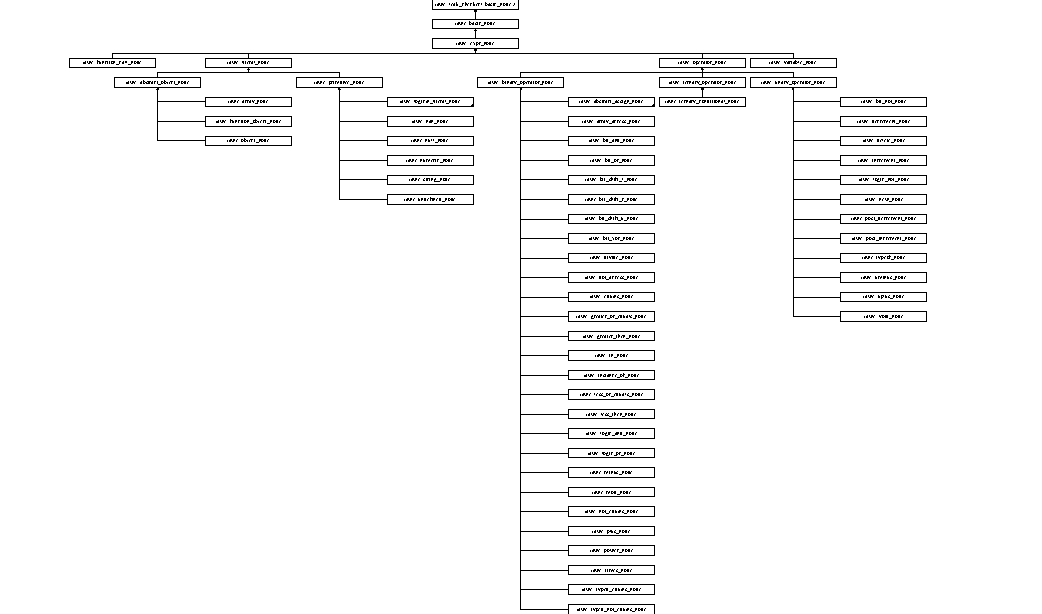
\includegraphics[height=8.258064cm]{classjawe_1_1expr__node}
\end{center}
\end{figure}
\subsection*{Public Member Functions}
\begin{DoxyCompactItemize}
\item 
\hyperlink{classjawe_1_1expr__node_a3b525868667d0354a7de8f79ad4e1111}{expr\+\_\+node} (std\+::string symbol)
\end{DoxyCompactItemize}
\subsection*{Additional Inherited Members}


\subsection{Constructor \& Destructor Documentation}
\mbox{\Hypertarget{classjawe_1_1expr__node_a3b525868667d0354a7de8f79ad4e1111}\label{classjawe_1_1expr__node_a3b525868667d0354a7de8f79ad4e1111}} 
\index{jawe\+::expr\+\_\+node@{jawe\+::expr\+\_\+node}!expr\+\_\+node@{expr\+\_\+node}}
\index{expr\+\_\+node@{expr\+\_\+node}!jawe\+::expr\+\_\+node@{jawe\+::expr\+\_\+node}}
\subsubsection{\texorpdfstring{expr\+\_\+node()}{expr\_node()}}
{\footnotesize\ttfamily expr\+\_\+node\+::expr\+\_\+node (\begin{DoxyParamCaption}\item[{std\+::string}]{symbol }\end{DoxyParamCaption})}



The documentation for this class was generated from the following files\+:\begin{DoxyCompactItemize}
\item 
include/syntax/abstract/\hyperlink{expr__node_8hpp}{expr\+\_\+node.\+hpp}\item 
src/syntax/abstract/\hyperlink{expr__node_8cpp}{expr\+\_\+node.\+cpp}\end{DoxyCompactItemize}

\hypertarget{classjawe_1_1false__node}{}\section{jawe\+:\+:false\+\_\+node Class Reference}
\label{classjawe_1_1false__node}\index{jawe\+::false\+\_\+node@{jawe\+::false\+\_\+node}}


{\ttfamily \#include $<$false\+\_\+node.\+hpp$>$}

Inheritance diagram for jawe\+:\+:false\+\_\+node\+:\begin{figure}[H]
\begin{center}
\leavevmode
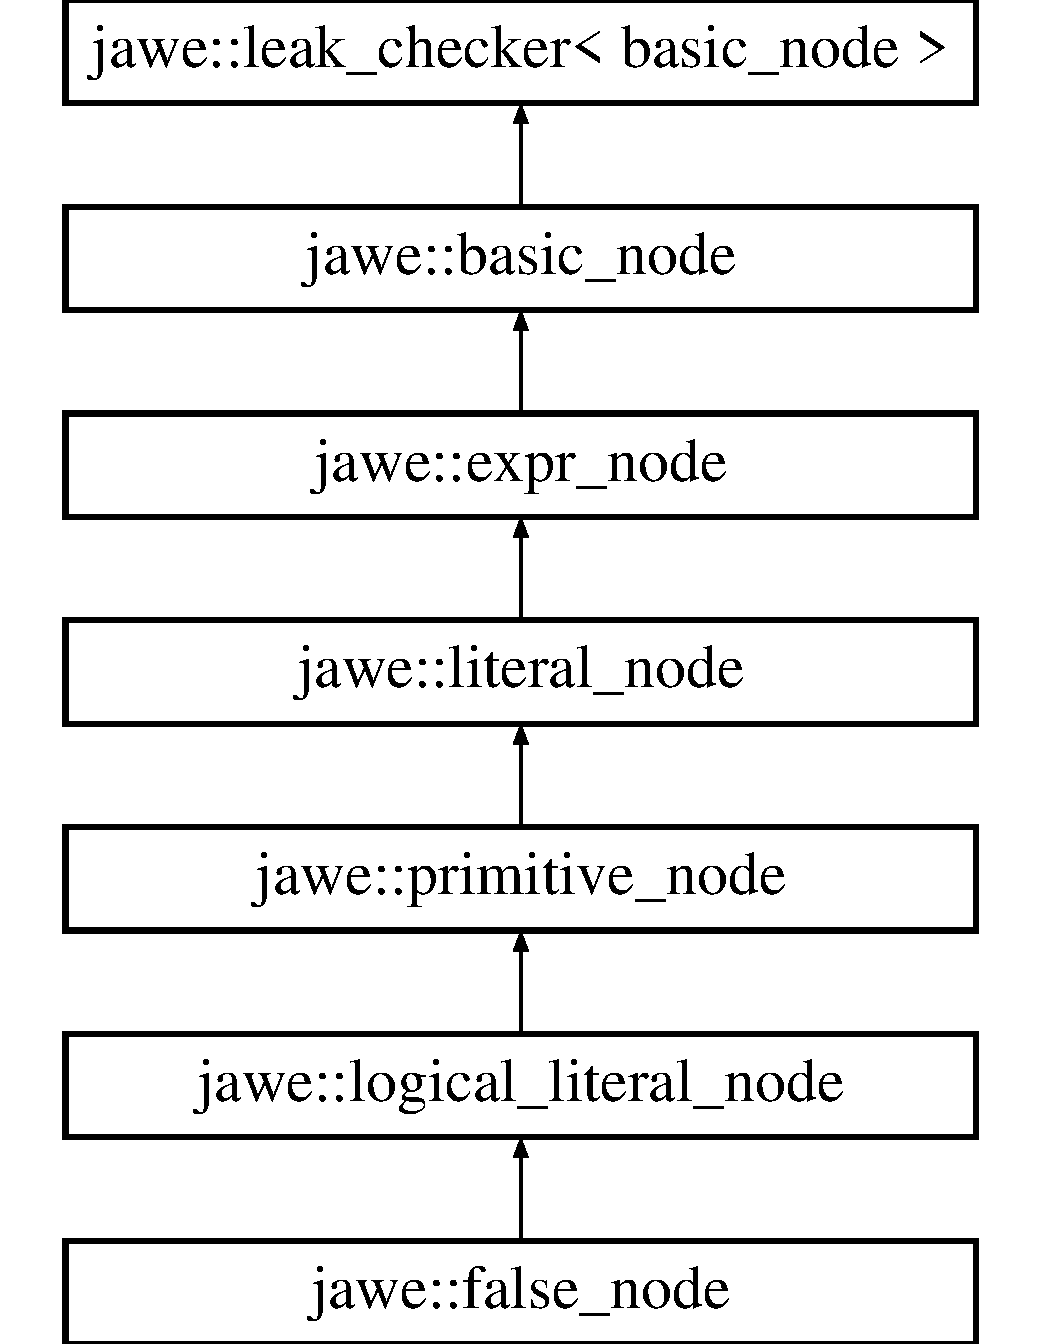
\includegraphics[height=7.000000cm]{classjawe_1_1false__node}
\end{center}
\end{figure}
\subsection*{Public Member Functions}
\begin{DoxyCompactItemize}
\item 
\hyperlink{classjawe_1_1false__node_aea4f5d3ffa7afceb4c1b0503dcfb7463}{false\+\_\+node} ()
\end{DoxyCompactItemize}
\subsection*{Additional Inherited Members}


\subsection{Constructor \& Destructor Documentation}
\mbox{\Hypertarget{classjawe_1_1false__node_aea4f5d3ffa7afceb4c1b0503dcfb7463}\label{classjawe_1_1false__node_aea4f5d3ffa7afceb4c1b0503dcfb7463}} 
\index{jawe\+::false\+\_\+node@{jawe\+::false\+\_\+node}!false\+\_\+node@{false\+\_\+node}}
\index{false\+\_\+node@{false\+\_\+node}!jawe\+::false\+\_\+node@{jawe\+::false\+\_\+node}}
\subsubsection{\texorpdfstring{false\+\_\+node()}{false\_node()}}
{\footnotesize\ttfamily false\+\_\+node\+::false\+\_\+node (\begin{DoxyParamCaption}{ }\end{DoxyParamCaption})}



The documentation for this class was generated from the following files\+:\begin{DoxyCompactItemize}
\item 
include/syntax/literals/\hyperlink{false__node_8hpp}{false\+\_\+node.\+hpp}\item 
src/syntax/literals/\hyperlink{false__node_8cpp}{false\+\_\+node.\+cpp}\end{DoxyCompactItemize}

\hypertarget{classjawe_1_1file__checker}{}\section{jawe\+:\+:file\+\_\+checker Class Reference}
\label{classjawe_1_1file__checker}\index{jawe\+::file\+\_\+checker@{jawe\+::file\+\_\+checker}}


{\ttfamily \#include $<$file\+\_\+checker.\+hpp$>$}

Inheritance diagram for jawe\+:\+:file\+\_\+checker\+:\begin{figure}[H]
\begin{center}
\leavevmode
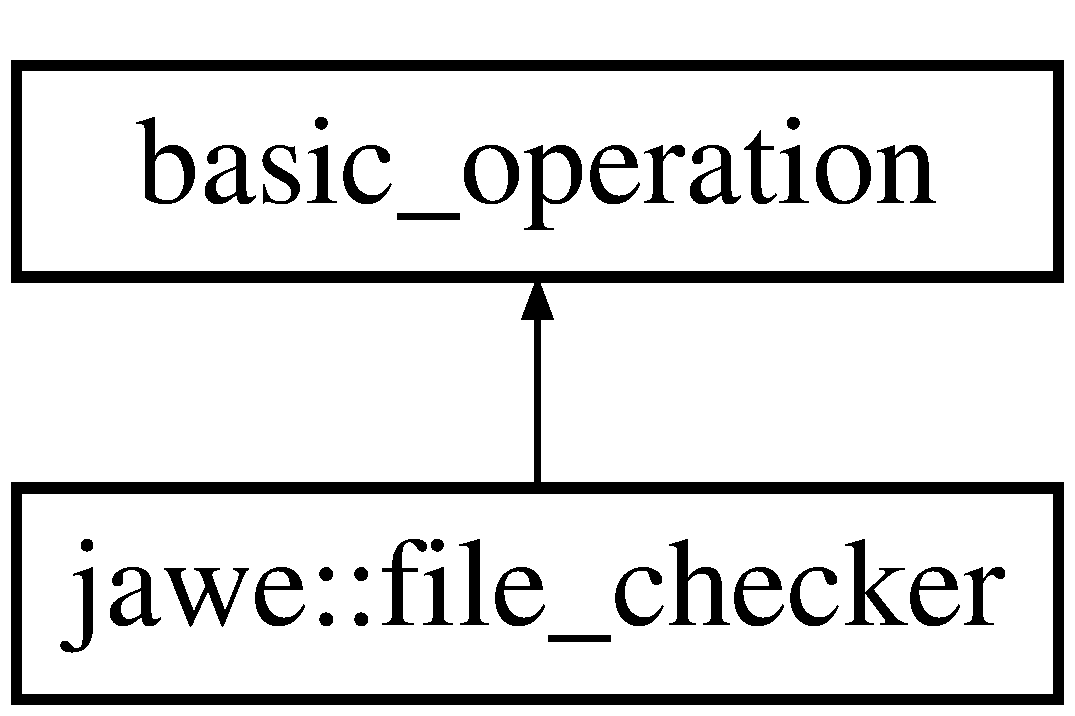
\includegraphics[height=2.000000cm]{classjawe_1_1file__checker}
\end{center}
\end{figure}
\subsection*{Public Member Functions}
\begin{DoxyCompactItemize}
\item 
void \hyperlink{classjawe_1_1file__checker_ae0f4f3a76e2d85024fd35bea0e119c0f}{run} () const
\end{DoxyCompactItemize}


\subsection{Member Function Documentation}
\mbox{\Hypertarget{classjawe_1_1file__checker_ae0f4f3a76e2d85024fd35bea0e119c0f}\label{classjawe_1_1file__checker_ae0f4f3a76e2d85024fd35bea0e119c0f}} 
\index{jawe\+::file\+\_\+checker@{jawe\+::file\+\_\+checker}!run@{run}}
\index{run@{run}!jawe\+::file\+\_\+checker@{jawe\+::file\+\_\+checker}}
\subsubsection{\texorpdfstring{run()}{run()}}
{\footnotesize\ttfamily void file\+\_\+checker\+::run (\begin{DoxyParamCaption}{ }\end{DoxyParamCaption}) const}



The documentation for this class was generated from the following files\+:\begin{DoxyCompactItemize}
\item 
include/operations/\hyperlink{file__checker_8hpp}{file\+\_\+checker.\+hpp}\item 
src/operations/\hyperlink{file__checker_8cpp}{file\+\_\+checker.\+cpp}\end{DoxyCompactItemize}

\hypertarget{classjawe_1_1for__node}{}\section{jawe\+:\+:for\+\_\+node Class Reference}
\label{classjawe_1_1for__node}\index{jawe\+::for\+\_\+node@{jawe\+::for\+\_\+node}}


{\ttfamily \#include $<$for\+\_\+node.\+hpp$>$}

Inheritance diagram for jawe\+:\+:for\+\_\+node\+:\begin{figure}[H]
\begin{center}
\leavevmode
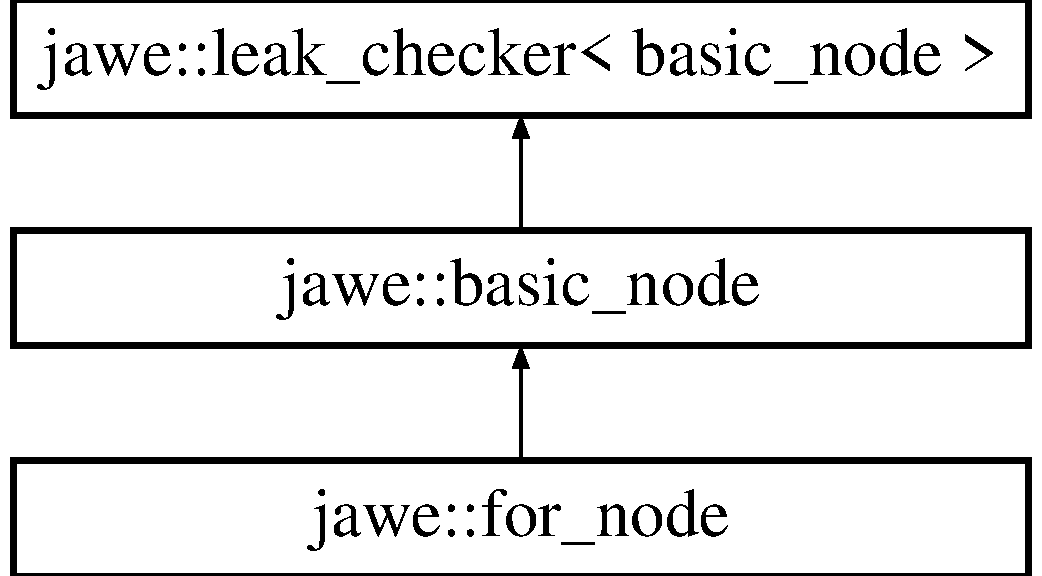
\includegraphics[height=3.000000cm]{classjawe_1_1for__node}
\end{center}
\end{figure}
\subsection*{Public Member Functions}
\begin{DoxyCompactItemize}
\item 
\hyperlink{classjawe_1_1for__node_a720114bf0a3a54234f0440b28bee76ac}{for\+\_\+node} (const \hyperlink{namespacejawe_a3f307481d921b6cbb50cc8511fc2b544}{shared\+\_\+node} \&, const \hyperlink{namespacejawe_a3f307481d921b6cbb50cc8511fc2b544}{shared\+\_\+node} \&, const \hyperlink{namespacejawe_a3f307481d921b6cbb50cc8511fc2b544}{shared\+\_\+node} \&, const \hyperlink{namespacejawe_a3f307481d921b6cbb50cc8511fc2b544}{shared\+\_\+node} \&)
\item 
\hyperlink{namespacejawe_a3f307481d921b6cbb50cc8511fc2b544}{shared\+\_\+node} \hyperlink{classjawe_1_1for__node_a5717876344a01dc22d0601f082f014e4}{get\+\_\+expr} () const
\item 
\hyperlink{namespacejawe_a3f307481d921b6cbb50cc8511fc2b544}{shared\+\_\+node} \hyperlink{classjawe_1_1for__node_a486a5ec435ae87654f63dd2fdca55093}{get\+\_\+body} () const
\item 
\hyperlink{namespacejawe_a3f307481d921b6cbb50cc8511fc2b544}{shared\+\_\+node} \hyperlink{classjawe_1_1for__node_af47b420f615e83103dc1035a76324db6}{get\+\_\+init} () const
\item 
\hyperlink{namespacejawe_a3f307481d921b6cbb50cc8511fc2b544}{shared\+\_\+node} \hyperlink{classjawe_1_1for__node_abc377eab368d131f41e184642ee9942d}{get\+\_\+post} () const
\end{DoxyCompactItemize}
\subsection*{Private Attributes}
\begin{DoxyCompactItemize}
\item 
\hyperlink{namespacejawe_a3f307481d921b6cbb50cc8511fc2b544}{shared\+\_\+node} \hyperlink{classjawe_1_1for__node_a3ede0b1860eb521ca4d3e0eef422bde9}{m\+\_\+init}
\item 
\hyperlink{namespacejawe_a3f307481d921b6cbb50cc8511fc2b544}{shared\+\_\+node} \hyperlink{classjawe_1_1for__node_a5b1999ad9e78b7d3773a6c1b8f74006f}{m\+\_\+cond}
\item 
\hyperlink{namespacejawe_a3f307481d921b6cbb50cc8511fc2b544}{shared\+\_\+node} \hyperlink{classjawe_1_1for__node_a3fe75e2c277af21538197a39a496492b}{m\+\_\+post}
\item 
\hyperlink{namespacejawe_a3f307481d921b6cbb50cc8511fc2b544}{shared\+\_\+node} \hyperlink{classjawe_1_1for__node_a64c9d22116feeae7c5a8f712483c2ad2}{m\+\_\+body}
\end{DoxyCompactItemize}
\subsection*{Additional Inherited Members}


\subsection{Constructor \& Destructor Documentation}
\mbox{\Hypertarget{classjawe_1_1for__node_a720114bf0a3a54234f0440b28bee76ac}\label{classjawe_1_1for__node_a720114bf0a3a54234f0440b28bee76ac}} 
\index{jawe\+::for\+\_\+node@{jawe\+::for\+\_\+node}!for\+\_\+node@{for\+\_\+node}}
\index{for\+\_\+node@{for\+\_\+node}!jawe\+::for\+\_\+node@{jawe\+::for\+\_\+node}}
\subsubsection{\texorpdfstring{for\+\_\+node()}{for\_node()}}
{\footnotesize\ttfamily for\+\_\+node\+::for\+\_\+node (\begin{DoxyParamCaption}\item[{const \hyperlink{namespacejawe_a3f307481d921b6cbb50cc8511fc2b544}{shared\+\_\+node} \&}]{init,  }\item[{const \hyperlink{namespacejawe_a3f307481d921b6cbb50cc8511fc2b544}{shared\+\_\+node} \&}]{cond,  }\item[{const \hyperlink{namespacejawe_a3f307481d921b6cbb50cc8511fc2b544}{shared\+\_\+node} \&}]{post,  }\item[{const \hyperlink{namespacejawe_a3f307481d921b6cbb50cc8511fc2b544}{shared\+\_\+node} \&}]{body }\end{DoxyParamCaption})}



\subsection{Member Function Documentation}
\mbox{\Hypertarget{classjawe_1_1for__node_a486a5ec435ae87654f63dd2fdca55093}\label{classjawe_1_1for__node_a486a5ec435ae87654f63dd2fdca55093}} 
\index{jawe\+::for\+\_\+node@{jawe\+::for\+\_\+node}!get\+\_\+body@{get\+\_\+body}}
\index{get\+\_\+body@{get\+\_\+body}!jawe\+::for\+\_\+node@{jawe\+::for\+\_\+node}}
\subsubsection{\texorpdfstring{get\+\_\+body()}{get\_body()}}
{\footnotesize\ttfamily \hyperlink{namespacejawe_a3f307481d921b6cbb50cc8511fc2b544}{shared\+\_\+node} for\+\_\+node\+::get\+\_\+body (\begin{DoxyParamCaption}{ }\end{DoxyParamCaption}) const}

\mbox{\Hypertarget{classjawe_1_1for__node_a5717876344a01dc22d0601f082f014e4}\label{classjawe_1_1for__node_a5717876344a01dc22d0601f082f014e4}} 
\index{jawe\+::for\+\_\+node@{jawe\+::for\+\_\+node}!get\+\_\+expr@{get\+\_\+expr}}
\index{get\+\_\+expr@{get\+\_\+expr}!jawe\+::for\+\_\+node@{jawe\+::for\+\_\+node}}
\subsubsection{\texorpdfstring{get\+\_\+expr()}{get\_expr()}}
{\footnotesize\ttfamily \hyperlink{namespacejawe_a3f307481d921b6cbb50cc8511fc2b544}{shared\+\_\+node} for\+\_\+node\+::get\+\_\+expr (\begin{DoxyParamCaption}{ }\end{DoxyParamCaption}) const}

\mbox{\Hypertarget{classjawe_1_1for__node_af47b420f615e83103dc1035a76324db6}\label{classjawe_1_1for__node_af47b420f615e83103dc1035a76324db6}} 
\index{jawe\+::for\+\_\+node@{jawe\+::for\+\_\+node}!get\+\_\+init@{get\+\_\+init}}
\index{get\+\_\+init@{get\+\_\+init}!jawe\+::for\+\_\+node@{jawe\+::for\+\_\+node}}
\subsubsection{\texorpdfstring{get\+\_\+init()}{get\_init()}}
{\footnotesize\ttfamily \hyperlink{namespacejawe_a3f307481d921b6cbb50cc8511fc2b544}{shared\+\_\+node} for\+\_\+node\+::get\+\_\+init (\begin{DoxyParamCaption}{ }\end{DoxyParamCaption}) const}

\mbox{\Hypertarget{classjawe_1_1for__node_abc377eab368d131f41e184642ee9942d}\label{classjawe_1_1for__node_abc377eab368d131f41e184642ee9942d}} 
\index{jawe\+::for\+\_\+node@{jawe\+::for\+\_\+node}!get\+\_\+post@{get\+\_\+post}}
\index{get\+\_\+post@{get\+\_\+post}!jawe\+::for\+\_\+node@{jawe\+::for\+\_\+node}}
\subsubsection{\texorpdfstring{get\+\_\+post()}{get\_post()}}
{\footnotesize\ttfamily \hyperlink{namespacejawe_a3f307481d921b6cbb50cc8511fc2b544}{shared\+\_\+node} for\+\_\+node\+::get\+\_\+post (\begin{DoxyParamCaption}{ }\end{DoxyParamCaption}) const}



\subsection{Member Data Documentation}
\mbox{\Hypertarget{classjawe_1_1for__node_a64c9d22116feeae7c5a8f712483c2ad2}\label{classjawe_1_1for__node_a64c9d22116feeae7c5a8f712483c2ad2}} 
\index{jawe\+::for\+\_\+node@{jawe\+::for\+\_\+node}!m\+\_\+body@{m\+\_\+body}}
\index{m\+\_\+body@{m\+\_\+body}!jawe\+::for\+\_\+node@{jawe\+::for\+\_\+node}}
\subsubsection{\texorpdfstring{m\+\_\+body}{m\_body}}
{\footnotesize\ttfamily \hyperlink{namespacejawe_a3f307481d921b6cbb50cc8511fc2b544}{shared\+\_\+node} jawe\+::for\+\_\+node\+::m\+\_\+body\hspace{0.3cm}{\ttfamily [private]}}

\mbox{\Hypertarget{classjawe_1_1for__node_a5b1999ad9e78b7d3773a6c1b8f74006f}\label{classjawe_1_1for__node_a5b1999ad9e78b7d3773a6c1b8f74006f}} 
\index{jawe\+::for\+\_\+node@{jawe\+::for\+\_\+node}!m\+\_\+cond@{m\+\_\+cond}}
\index{m\+\_\+cond@{m\+\_\+cond}!jawe\+::for\+\_\+node@{jawe\+::for\+\_\+node}}
\subsubsection{\texorpdfstring{m\+\_\+cond}{m\_cond}}
{\footnotesize\ttfamily \hyperlink{namespacejawe_a3f307481d921b6cbb50cc8511fc2b544}{shared\+\_\+node} jawe\+::for\+\_\+node\+::m\+\_\+cond\hspace{0.3cm}{\ttfamily [private]}}

\mbox{\Hypertarget{classjawe_1_1for__node_a3ede0b1860eb521ca4d3e0eef422bde9}\label{classjawe_1_1for__node_a3ede0b1860eb521ca4d3e0eef422bde9}} 
\index{jawe\+::for\+\_\+node@{jawe\+::for\+\_\+node}!m\+\_\+init@{m\+\_\+init}}
\index{m\+\_\+init@{m\+\_\+init}!jawe\+::for\+\_\+node@{jawe\+::for\+\_\+node}}
\subsubsection{\texorpdfstring{m\+\_\+init}{m\_init}}
{\footnotesize\ttfamily \hyperlink{namespacejawe_a3f307481d921b6cbb50cc8511fc2b544}{shared\+\_\+node} jawe\+::for\+\_\+node\+::m\+\_\+init\hspace{0.3cm}{\ttfamily [private]}}

\mbox{\Hypertarget{classjawe_1_1for__node_a3fe75e2c277af21538197a39a496492b}\label{classjawe_1_1for__node_a3fe75e2c277af21538197a39a496492b}} 
\index{jawe\+::for\+\_\+node@{jawe\+::for\+\_\+node}!m\+\_\+post@{m\+\_\+post}}
\index{m\+\_\+post@{m\+\_\+post}!jawe\+::for\+\_\+node@{jawe\+::for\+\_\+node}}
\subsubsection{\texorpdfstring{m\+\_\+post}{m\_post}}
{\footnotesize\ttfamily \hyperlink{namespacejawe_a3f307481d921b6cbb50cc8511fc2b544}{shared\+\_\+node} jawe\+::for\+\_\+node\+::m\+\_\+post\hspace{0.3cm}{\ttfamily [private]}}



The documentation for this class was generated from the following files\+:\begin{DoxyCompactItemize}
\item 
include/syntax/control\+\_\+flow/\hyperlink{for__node_8hpp}{for\+\_\+node.\+hpp}\item 
src/syntax/control\+\_\+flow/\hyperlink{for__node_8cpp}{for\+\_\+node.\+cpp}\end{DoxyCompactItemize}

\hypertarget{classjawe_1_1function__call__node}{}\section{jawe\+:\+:function\+\_\+call\+\_\+node Class Reference}
\label{classjawe_1_1function__call__node}\index{jawe\+::function\+\_\+call\+\_\+node@{jawe\+::function\+\_\+call\+\_\+node}}


{\ttfamily \#include $<$function\+\_\+call\+\_\+node.\+hpp$>$}

Inheritance diagram for jawe\+:\+:function\+\_\+call\+\_\+node\+:\begin{figure}[H]
\begin{center}
\leavevmode
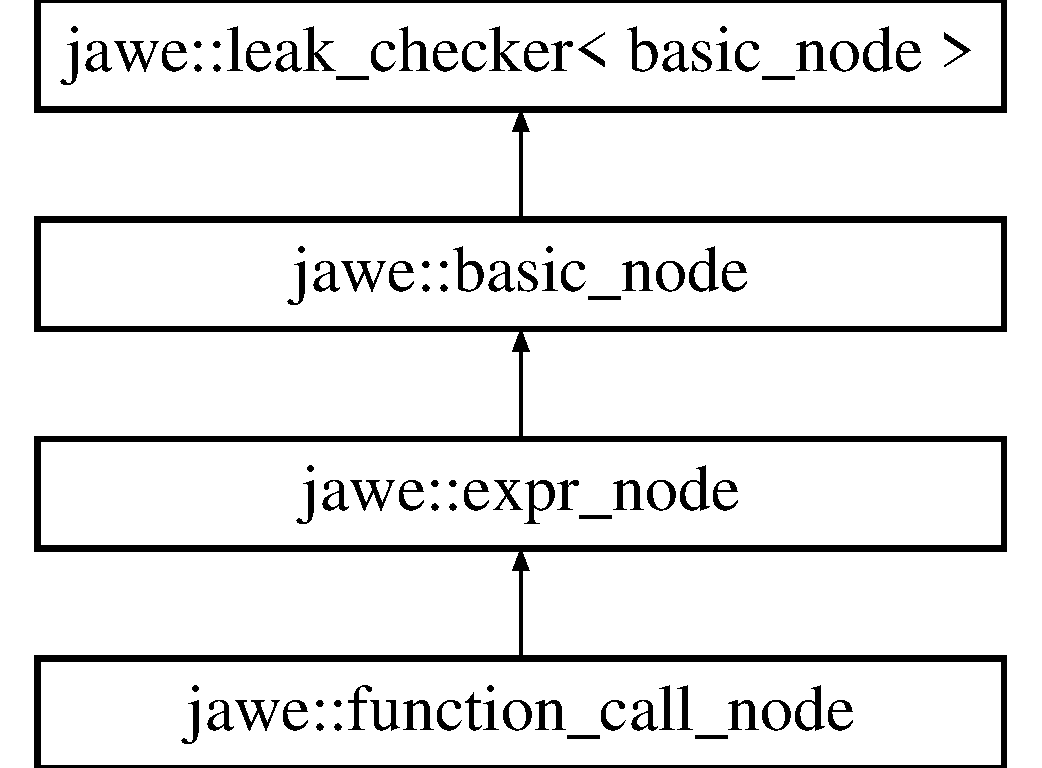
\includegraphics[height=4.000000cm]{classjawe_1_1function__call__node}
\end{center}
\end{figure}
\subsection*{Public Member Functions}
\begin{DoxyCompactItemize}
\item 
\hyperlink{classjawe_1_1function__call__node_a2c3a421053dc63b17efef188f4460c19}{function\+\_\+call\+\_\+node} (const \hyperlink{namespacejawe_a3f307481d921b6cbb50cc8511fc2b544}{shared\+\_\+node} \&)
\item 
\hyperlink{classjawe_1_1function__call__node_afdec8b2a9ab5db923eac27653e50a5f7}{function\+\_\+call\+\_\+node} (const \hyperlink{namespacejawe_a3f307481d921b6cbb50cc8511fc2b544}{shared\+\_\+node} \&, const std\+::vector$<$ \hyperlink{namespacejawe_a3f307481d921b6cbb50cc8511fc2b544}{shared\+\_\+node} $>$ \&)
\item 
void \hyperlink{classjawe_1_1function__call__node_a1eb6906152cb0372b5e13da9106afe4b}{push\+\_\+back} (const \hyperlink{namespacejawe_a3f307481d921b6cbb50cc8511fc2b544}{shared\+\_\+node} \&)
\item 
\hyperlink{namespacejawe_a3f307481d921b6cbb50cc8511fc2b544}{shared\+\_\+node} \hyperlink{classjawe_1_1function__call__node_ab9ce2d744923acc3d323605b155d4d78}{get\+\_\+expr} ()
\item 
std\+::vector$<$ \hyperlink{namespacejawe_a3f307481d921b6cbb50cc8511fc2b544}{shared\+\_\+node} $>$ \hyperlink{classjawe_1_1function__call__node_a9c8b1370713757589fc05f68eb14aa3e}{get\+\_\+args} ()
\end{DoxyCompactItemize}
\subsection*{Private Attributes}
\begin{DoxyCompactItemize}
\item 
\hyperlink{namespacejawe_a3f307481d921b6cbb50cc8511fc2b544}{shared\+\_\+node} \hyperlink{classjawe_1_1function__call__node_a5f27859d75f8f078a169afd6abf574ba}{m\+\_\+expr}
\item 
std\+::vector$<$ \hyperlink{namespacejawe_a3f307481d921b6cbb50cc8511fc2b544}{shared\+\_\+node} $>$ \hyperlink{classjawe_1_1function__call__node_aab5c174a179c885492cc929e6cebe2ee}{m\+\_\+args}
\end{DoxyCompactItemize}
\subsection*{Additional Inherited Members}


\subsection{Constructor \& Destructor Documentation}
\mbox{\Hypertarget{classjawe_1_1function__call__node_a2c3a421053dc63b17efef188f4460c19}\label{classjawe_1_1function__call__node_a2c3a421053dc63b17efef188f4460c19}} 
\index{jawe\+::function\+\_\+call\+\_\+node@{jawe\+::function\+\_\+call\+\_\+node}!function\+\_\+call\+\_\+node@{function\+\_\+call\+\_\+node}}
\index{function\+\_\+call\+\_\+node@{function\+\_\+call\+\_\+node}!jawe\+::function\+\_\+call\+\_\+node@{jawe\+::function\+\_\+call\+\_\+node}}
\subsubsection{\texorpdfstring{function\+\_\+call\+\_\+node()}{function\_call\_node()}\hspace{0.1cm}{\footnotesize\ttfamily [1/2]}}
{\footnotesize\ttfamily function\+\_\+call\+\_\+node\+::function\+\_\+call\+\_\+node (\begin{DoxyParamCaption}\item[{const \hyperlink{namespacejawe_a3f307481d921b6cbb50cc8511fc2b544}{shared\+\_\+node} \&}]{expr }\end{DoxyParamCaption})}

\mbox{\Hypertarget{classjawe_1_1function__call__node_afdec8b2a9ab5db923eac27653e50a5f7}\label{classjawe_1_1function__call__node_afdec8b2a9ab5db923eac27653e50a5f7}} 
\index{jawe\+::function\+\_\+call\+\_\+node@{jawe\+::function\+\_\+call\+\_\+node}!function\+\_\+call\+\_\+node@{function\+\_\+call\+\_\+node}}
\index{function\+\_\+call\+\_\+node@{function\+\_\+call\+\_\+node}!jawe\+::function\+\_\+call\+\_\+node@{jawe\+::function\+\_\+call\+\_\+node}}
\subsubsection{\texorpdfstring{function\+\_\+call\+\_\+node()}{function\_call\_node()}\hspace{0.1cm}{\footnotesize\ttfamily [2/2]}}
{\footnotesize\ttfamily function\+\_\+call\+\_\+node\+::function\+\_\+call\+\_\+node (\begin{DoxyParamCaption}\item[{const \hyperlink{namespacejawe_a3f307481d921b6cbb50cc8511fc2b544}{shared\+\_\+node} \&}]{expr,  }\item[{const std\+::vector$<$ \hyperlink{namespacejawe_a3f307481d921b6cbb50cc8511fc2b544}{shared\+\_\+node} $>$ \&}]{args }\end{DoxyParamCaption})}



\subsection{Member Function Documentation}
\mbox{\Hypertarget{classjawe_1_1function__call__node_a9c8b1370713757589fc05f68eb14aa3e}\label{classjawe_1_1function__call__node_a9c8b1370713757589fc05f68eb14aa3e}} 
\index{jawe\+::function\+\_\+call\+\_\+node@{jawe\+::function\+\_\+call\+\_\+node}!get\+\_\+args@{get\+\_\+args}}
\index{get\+\_\+args@{get\+\_\+args}!jawe\+::function\+\_\+call\+\_\+node@{jawe\+::function\+\_\+call\+\_\+node}}
\subsubsection{\texorpdfstring{get\+\_\+args()}{get\_args()}}
{\footnotesize\ttfamily std\+::vector$<$ \hyperlink{namespacejawe_a3f307481d921b6cbb50cc8511fc2b544}{shared\+\_\+node} $>$ function\+\_\+call\+\_\+node\+::get\+\_\+args (\begin{DoxyParamCaption}{ }\end{DoxyParamCaption})}

\mbox{\Hypertarget{classjawe_1_1function__call__node_ab9ce2d744923acc3d323605b155d4d78}\label{classjawe_1_1function__call__node_ab9ce2d744923acc3d323605b155d4d78}} 
\index{jawe\+::function\+\_\+call\+\_\+node@{jawe\+::function\+\_\+call\+\_\+node}!get\+\_\+expr@{get\+\_\+expr}}
\index{get\+\_\+expr@{get\+\_\+expr}!jawe\+::function\+\_\+call\+\_\+node@{jawe\+::function\+\_\+call\+\_\+node}}
\subsubsection{\texorpdfstring{get\+\_\+expr()}{get\_expr()}}
{\footnotesize\ttfamily \hyperlink{namespacejawe_a3f307481d921b6cbb50cc8511fc2b544}{shared\+\_\+node} function\+\_\+call\+\_\+node\+::get\+\_\+expr (\begin{DoxyParamCaption}{ }\end{DoxyParamCaption})}

\mbox{\Hypertarget{classjawe_1_1function__call__node_a1eb6906152cb0372b5e13da9106afe4b}\label{classjawe_1_1function__call__node_a1eb6906152cb0372b5e13da9106afe4b}} 
\index{jawe\+::function\+\_\+call\+\_\+node@{jawe\+::function\+\_\+call\+\_\+node}!push\+\_\+back@{push\+\_\+back}}
\index{push\+\_\+back@{push\+\_\+back}!jawe\+::function\+\_\+call\+\_\+node@{jawe\+::function\+\_\+call\+\_\+node}}
\subsubsection{\texorpdfstring{push\+\_\+back()}{push\_back()}}
{\footnotesize\ttfamily void function\+\_\+call\+\_\+node\+::push\+\_\+back (\begin{DoxyParamCaption}\item[{const \hyperlink{namespacejawe_a3f307481d921b6cbb50cc8511fc2b544}{shared\+\_\+node} \&}]{expr }\end{DoxyParamCaption})}



\subsection{Member Data Documentation}
\mbox{\Hypertarget{classjawe_1_1function__call__node_aab5c174a179c885492cc929e6cebe2ee}\label{classjawe_1_1function__call__node_aab5c174a179c885492cc929e6cebe2ee}} 
\index{jawe\+::function\+\_\+call\+\_\+node@{jawe\+::function\+\_\+call\+\_\+node}!m\+\_\+args@{m\+\_\+args}}
\index{m\+\_\+args@{m\+\_\+args}!jawe\+::function\+\_\+call\+\_\+node@{jawe\+::function\+\_\+call\+\_\+node}}
\subsubsection{\texorpdfstring{m\+\_\+args}{m\_args}}
{\footnotesize\ttfamily std\+::vector$<$\hyperlink{namespacejawe_a3f307481d921b6cbb50cc8511fc2b544}{shared\+\_\+node}$>$ jawe\+::function\+\_\+call\+\_\+node\+::m\+\_\+args\hspace{0.3cm}{\ttfamily [private]}}

\mbox{\Hypertarget{classjawe_1_1function__call__node_a5f27859d75f8f078a169afd6abf574ba}\label{classjawe_1_1function__call__node_a5f27859d75f8f078a169afd6abf574ba}} 
\index{jawe\+::function\+\_\+call\+\_\+node@{jawe\+::function\+\_\+call\+\_\+node}!m\+\_\+expr@{m\+\_\+expr}}
\index{m\+\_\+expr@{m\+\_\+expr}!jawe\+::function\+\_\+call\+\_\+node@{jawe\+::function\+\_\+call\+\_\+node}}
\subsubsection{\texorpdfstring{m\+\_\+expr}{m\_expr}}
{\footnotesize\ttfamily \hyperlink{namespacejawe_a3f307481d921b6cbb50cc8511fc2b544}{shared\+\_\+node} jawe\+::function\+\_\+call\+\_\+node\+::m\+\_\+expr\hspace{0.3cm}{\ttfamily [private]}}



The documentation for this class was generated from the following files\+:\begin{DoxyCompactItemize}
\item 
include/syntax/operators/\hyperlink{function__call__node_8hpp}{function\+\_\+call\+\_\+node.\+hpp}\item 
src/syntax/operators/\hyperlink{function__call__node_8cpp}{function\+\_\+call\+\_\+node.\+cpp}\end{DoxyCompactItemize}

\hypertarget{classjawe_1_1function__declaration__node}{}\section{jawe\+:\+:function\+\_\+declaration\+\_\+node Class Reference}
\label{classjawe_1_1function__declaration__node}\index{jawe\+::function\+\_\+declaration\+\_\+node@{jawe\+::function\+\_\+declaration\+\_\+node}}


{\ttfamily \#include $<$function\+\_\+declaration\+\_\+node.\+hpp$>$}

Inheritance diagram for jawe\+:\+:function\+\_\+declaration\+\_\+node\+:\begin{figure}[H]
\begin{center}
\leavevmode
\includegraphics[height=3.000000cm]{classjawe_1_1function__declaration__node}
\end{center}
\end{figure}
\subsection*{Public Member Functions}
\begin{DoxyCompactItemize}
\item 
\hyperlink{classjawe_1_1function__declaration__node_ac28b6a6e48b90529b7fda41db75228d5}{function\+\_\+declaration\+\_\+node} (std\+::string, const \hyperlink{namespacejawe_a3f307481d921b6cbb50cc8511fc2b544}{shared\+\_\+node} \&)
\item 
\hyperlink{namespacejawe_a3f307481d921b6cbb50cc8511fc2b544}{shared\+\_\+node} \hyperlink{classjawe_1_1function__declaration__node_a012175493728b93d76b640d81d457887}{get\+\_\+body} ()
\item 
\hyperlink{namespacejawe_a3f307481d921b6cbb50cc8511fc2b544}{shared\+\_\+node} \hyperlink{classjawe_1_1function__declaration__node_a94a22b3f65e84c0b5dbf3a328c622035}{get\+\_\+function\+\_\+object} ()
\item 
std\+::string \hyperlink{classjawe_1_1function__declaration__node_a14acad1583a39308f099a9af49c16552}{get\+\_\+name} () const
\end{DoxyCompactItemize}
\subsection*{Private Attributes}
\begin{DoxyCompactItemize}
\item 
std\+::string \hyperlink{classjawe_1_1function__declaration__node_a1766e81709b60ebfddc3806728ec2d0c}{m\+\_\+name}
\item 
\hyperlink{namespacejawe_a3f307481d921b6cbb50cc8511fc2b544}{shared\+\_\+node} \hyperlink{classjawe_1_1function__declaration__node_a4b9bacead9449c28465ae3e8062cedd2}{m\+\_\+function\+\_\+object}
\end{DoxyCompactItemize}
\subsection*{Additional Inherited Members}


\subsection{Constructor \& Destructor Documentation}
\mbox{\Hypertarget{classjawe_1_1function__declaration__node_ac28b6a6e48b90529b7fda41db75228d5}\label{classjawe_1_1function__declaration__node_ac28b6a6e48b90529b7fda41db75228d5}} 
\index{jawe\+::function\+\_\+declaration\+\_\+node@{jawe\+::function\+\_\+declaration\+\_\+node}!function\+\_\+declaration\+\_\+node@{function\+\_\+declaration\+\_\+node}}
\index{function\+\_\+declaration\+\_\+node@{function\+\_\+declaration\+\_\+node}!jawe\+::function\+\_\+declaration\+\_\+node@{jawe\+::function\+\_\+declaration\+\_\+node}}
\subsubsection{\texorpdfstring{function\+\_\+declaration\+\_\+node()}{function\_declaration\_node()}}
{\footnotesize\ttfamily function\+\_\+declaration\+\_\+node\+::function\+\_\+declaration\+\_\+node (\begin{DoxyParamCaption}\item[{std\+::string}]{name,  }\item[{const \hyperlink{namespacejawe_a3f307481d921b6cbb50cc8511fc2b544}{shared\+\_\+node} \&}]{f }\end{DoxyParamCaption})}



\subsection{Member Function Documentation}
\mbox{\Hypertarget{classjawe_1_1function__declaration__node_a012175493728b93d76b640d81d457887}\label{classjawe_1_1function__declaration__node_a012175493728b93d76b640d81d457887}} 
\index{jawe\+::function\+\_\+declaration\+\_\+node@{jawe\+::function\+\_\+declaration\+\_\+node}!get\+\_\+body@{get\+\_\+body}}
\index{get\+\_\+body@{get\+\_\+body}!jawe\+::function\+\_\+declaration\+\_\+node@{jawe\+::function\+\_\+declaration\+\_\+node}}
\subsubsection{\texorpdfstring{get\+\_\+body()}{get\_body()}}
{\footnotesize\ttfamily \hyperlink{namespacejawe_a3f307481d921b6cbb50cc8511fc2b544}{shared\+\_\+node} function\+\_\+declaration\+\_\+node\+::get\+\_\+body (\begin{DoxyParamCaption}{ }\end{DoxyParamCaption})}

\mbox{\Hypertarget{classjawe_1_1function__declaration__node_a94a22b3f65e84c0b5dbf3a328c622035}\label{classjawe_1_1function__declaration__node_a94a22b3f65e84c0b5dbf3a328c622035}} 
\index{jawe\+::function\+\_\+declaration\+\_\+node@{jawe\+::function\+\_\+declaration\+\_\+node}!get\+\_\+function\+\_\+object@{get\+\_\+function\+\_\+object}}
\index{get\+\_\+function\+\_\+object@{get\+\_\+function\+\_\+object}!jawe\+::function\+\_\+declaration\+\_\+node@{jawe\+::function\+\_\+declaration\+\_\+node}}
\subsubsection{\texorpdfstring{get\+\_\+function\+\_\+object()}{get\_function\_object()}}
{\footnotesize\ttfamily \hyperlink{namespacejawe_a3f307481d921b6cbb50cc8511fc2b544}{shared\+\_\+node} function\+\_\+declaration\+\_\+node\+::get\+\_\+function\+\_\+object (\begin{DoxyParamCaption}{ }\end{DoxyParamCaption})}

\mbox{\Hypertarget{classjawe_1_1function__declaration__node_a14acad1583a39308f099a9af49c16552}\label{classjawe_1_1function__declaration__node_a14acad1583a39308f099a9af49c16552}} 
\index{jawe\+::function\+\_\+declaration\+\_\+node@{jawe\+::function\+\_\+declaration\+\_\+node}!get\+\_\+name@{get\+\_\+name}}
\index{get\+\_\+name@{get\+\_\+name}!jawe\+::function\+\_\+declaration\+\_\+node@{jawe\+::function\+\_\+declaration\+\_\+node}}
\subsubsection{\texorpdfstring{get\+\_\+name()}{get\_name()}}
{\footnotesize\ttfamily std\+::string function\+\_\+declaration\+\_\+node\+::get\+\_\+name (\begin{DoxyParamCaption}{ }\end{DoxyParamCaption}) const}



\subsection{Member Data Documentation}
\mbox{\Hypertarget{classjawe_1_1function__declaration__node_a4b9bacead9449c28465ae3e8062cedd2}\label{classjawe_1_1function__declaration__node_a4b9bacead9449c28465ae3e8062cedd2}} 
\index{jawe\+::function\+\_\+declaration\+\_\+node@{jawe\+::function\+\_\+declaration\+\_\+node}!m\+\_\+function\+\_\+object@{m\+\_\+function\+\_\+object}}
\index{m\+\_\+function\+\_\+object@{m\+\_\+function\+\_\+object}!jawe\+::function\+\_\+declaration\+\_\+node@{jawe\+::function\+\_\+declaration\+\_\+node}}
\subsubsection{\texorpdfstring{m\+\_\+function\+\_\+object}{m\_function\_object}}
{\footnotesize\ttfamily \hyperlink{namespacejawe_a3f307481d921b6cbb50cc8511fc2b544}{shared\+\_\+node} jawe\+::function\+\_\+declaration\+\_\+node\+::m\+\_\+function\+\_\+object\hspace{0.3cm}{\ttfamily [private]}}

\mbox{\Hypertarget{classjawe_1_1function__declaration__node_a1766e81709b60ebfddc3806728ec2d0c}\label{classjawe_1_1function__declaration__node_a1766e81709b60ebfddc3806728ec2d0c}} 
\index{jawe\+::function\+\_\+declaration\+\_\+node@{jawe\+::function\+\_\+declaration\+\_\+node}!m\+\_\+name@{m\+\_\+name}}
\index{m\+\_\+name@{m\+\_\+name}!jawe\+::function\+\_\+declaration\+\_\+node@{jawe\+::function\+\_\+declaration\+\_\+node}}
\subsubsection{\texorpdfstring{m\+\_\+name}{m\_name}}
{\footnotesize\ttfamily std\+::string jawe\+::function\+\_\+declaration\+\_\+node\+::m\+\_\+name\hspace{0.3cm}{\ttfamily [private]}}



The documentation for this class was generated from the following files\+:\begin{DoxyCompactItemize}
\item 
include/syntax/variables/\hyperlink{function__declaration__node_8hpp}{function\+\_\+declaration\+\_\+node.\+hpp}\item 
src/syntax/variables/\hyperlink{function__declaration__node_8cpp}{function\+\_\+declaration\+\_\+node.\+cpp}\end{DoxyCompactItemize}

\hypertarget{classjawe_1_1function__object__node}{}\section{jawe\+:\+:function\+\_\+object\+\_\+node Class Reference}
\label{classjawe_1_1function__object__node}\index{jawe\+::function\+\_\+object\+\_\+node@{jawe\+::function\+\_\+object\+\_\+node}}


{\ttfamily \#include $<$function\+\_\+object\+\_\+node.\+hpp$>$}

Inheritance diagram for jawe\+:\+:function\+\_\+object\+\_\+node\+:\begin{figure}[H]
\begin{center}
\leavevmode
\includegraphics[height=6.000000cm]{classjawe_1_1function__object__node}
\end{center}
\end{figure}
\subsection*{Public Member Functions}
\begin{DoxyCompactItemize}
\item 
\hyperlink{classjawe_1_1function__object__node_ae7bff56873ee72d59fd2aa248c6af950}{function\+\_\+object\+\_\+node} (const std\+::vector$<$ std\+::string $>$ \&, const \hyperlink{namespacejawe_a3f307481d921b6cbb50cc8511fc2b544}{shared\+\_\+node} \&, std\+::string)
\item 
\hyperlink{namespacejawe_a3f307481d921b6cbb50cc8511fc2b544}{shared\+\_\+node} \hyperlink{classjawe_1_1function__object__node_aa8c0d3afcc6aaf08fc4b1849a8858299}{get\+\_\+body} ()
\item 
std\+::vector$<$ std\+::string $>$ \hyperlink{classjawe_1_1function__object__node_a70cac84994ab03b0bf6738b5916ccb0a}{get\+\_\+args} ()
\end{DoxyCompactItemize}
\subsection*{Private Attributes}
\begin{DoxyCompactItemize}
\item 
std\+::vector$<$ std\+::string $>$ \hyperlink{classjawe_1_1function__object__node_a1ae62495879cfec59334e976286b3e50}{m\+\_\+args}
\item 
\hyperlink{namespacejawe_a3f307481d921b6cbb50cc8511fc2b544}{shared\+\_\+node} \hyperlink{classjawe_1_1function__object__node_a9902f571f4149af4cf41034c14209005}{m\+\_\+body}
\end{DoxyCompactItemize}
\subsection*{Additional Inherited Members}


\subsection{Constructor \& Destructor Documentation}
\mbox{\Hypertarget{classjawe_1_1function__object__node_ae7bff56873ee72d59fd2aa248c6af950}\label{classjawe_1_1function__object__node_ae7bff56873ee72d59fd2aa248c6af950}} 
\index{jawe\+::function\+\_\+object\+\_\+node@{jawe\+::function\+\_\+object\+\_\+node}!function\+\_\+object\+\_\+node@{function\+\_\+object\+\_\+node}}
\index{function\+\_\+object\+\_\+node@{function\+\_\+object\+\_\+node}!jawe\+::function\+\_\+object\+\_\+node@{jawe\+::function\+\_\+object\+\_\+node}}
\subsubsection{\texorpdfstring{function\+\_\+object\+\_\+node()}{function\_object\_node()}}
{\footnotesize\ttfamily function\+\_\+object\+\_\+node\+::function\+\_\+object\+\_\+node (\begin{DoxyParamCaption}\item[{const std\+::vector$<$ std\+::string $>$ \&}]{args,  }\item[{const \hyperlink{namespacejawe_a3f307481d921b6cbb50cc8511fc2b544}{shared\+\_\+node} \&}]{body,  }\item[{std\+::string}]{symbol }\end{DoxyParamCaption})}



\subsection{Member Function Documentation}
\mbox{\Hypertarget{classjawe_1_1function__object__node_a70cac84994ab03b0bf6738b5916ccb0a}\label{classjawe_1_1function__object__node_a70cac84994ab03b0bf6738b5916ccb0a}} 
\index{jawe\+::function\+\_\+object\+\_\+node@{jawe\+::function\+\_\+object\+\_\+node}!get\+\_\+args@{get\+\_\+args}}
\index{get\+\_\+args@{get\+\_\+args}!jawe\+::function\+\_\+object\+\_\+node@{jawe\+::function\+\_\+object\+\_\+node}}
\subsubsection{\texorpdfstring{get\+\_\+args()}{get\_args()}}
{\footnotesize\ttfamily std\+::vector$<$ std\+::string $>$ function\+\_\+object\+\_\+node\+::get\+\_\+args (\begin{DoxyParamCaption}{ }\end{DoxyParamCaption})}

\mbox{\Hypertarget{classjawe_1_1function__object__node_aa8c0d3afcc6aaf08fc4b1849a8858299}\label{classjawe_1_1function__object__node_aa8c0d3afcc6aaf08fc4b1849a8858299}} 
\index{jawe\+::function\+\_\+object\+\_\+node@{jawe\+::function\+\_\+object\+\_\+node}!get\+\_\+body@{get\+\_\+body}}
\index{get\+\_\+body@{get\+\_\+body}!jawe\+::function\+\_\+object\+\_\+node@{jawe\+::function\+\_\+object\+\_\+node}}
\subsubsection{\texorpdfstring{get\+\_\+body()}{get\_body()}}
{\footnotesize\ttfamily \hyperlink{namespacejawe_a3f307481d921b6cbb50cc8511fc2b544}{shared\+\_\+node} function\+\_\+object\+\_\+node\+::get\+\_\+body (\begin{DoxyParamCaption}{ }\end{DoxyParamCaption})}



\subsection{Member Data Documentation}
\mbox{\Hypertarget{classjawe_1_1function__object__node_a1ae62495879cfec59334e976286b3e50}\label{classjawe_1_1function__object__node_a1ae62495879cfec59334e976286b3e50}} 
\index{jawe\+::function\+\_\+object\+\_\+node@{jawe\+::function\+\_\+object\+\_\+node}!m\+\_\+args@{m\+\_\+args}}
\index{m\+\_\+args@{m\+\_\+args}!jawe\+::function\+\_\+object\+\_\+node@{jawe\+::function\+\_\+object\+\_\+node}}
\subsubsection{\texorpdfstring{m\+\_\+args}{m\_args}}
{\footnotesize\ttfamily std\+::vector$<$std\+::string$>$ jawe\+::function\+\_\+object\+\_\+node\+::m\+\_\+args\hspace{0.3cm}{\ttfamily [private]}}

\mbox{\Hypertarget{classjawe_1_1function__object__node_a9902f571f4149af4cf41034c14209005}\label{classjawe_1_1function__object__node_a9902f571f4149af4cf41034c14209005}} 
\index{jawe\+::function\+\_\+object\+\_\+node@{jawe\+::function\+\_\+object\+\_\+node}!m\+\_\+body@{m\+\_\+body}}
\index{m\+\_\+body@{m\+\_\+body}!jawe\+::function\+\_\+object\+\_\+node@{jawe\+::function\+\_\+object\+\_\+node}}
\subsubsection{\texorpdfstring{m\+\_\+body}{m\_body}}
{\footnotesize\ttfamily \hyperlink{namespacejawe_a3f307481d921b6cbb50cc8511fc2b544}{shared\+\_\+node} jawe\+::function\+\_\+object\+\_\+node\+::m\+\_\+body\hspace{0.3cm}{\ttfamily [private]}}



The documentation for this class was generated from the following files\+:\begin{DoxyCompactItemize}
\item 
include/syntax/literals/\hyperlink{function__object__node_8hpp}{function\+\_\+object\+\_\+node.\+hpp}\item 
src/syntax/literals/\hyperlink{function__object__node_8cpp}{function\+\_\+object\+\_\+node.\+cpp}\end{DoxyCompactItemize}

\hypertarget{classjawe_1_1greater__or__equals__node}{}\section{jawe\+:\+:greater\+\_\+or\+\_\+equals\+\_\+node Class Reference}
\label{classjawe_1_1greater__or__equals__node}\index{jawe\+::greater\+\_\+or\+\_\+equals\+\_\+node@{jawe\+::greater\+\_\+or\+\_\+equals\+\_\+node}}


{\ttfamily \#include $<$greater\+\_\+or\+\_\+equals\+\_\+node.\+hpp$>$}

Inheritance diagram for jawe\+:\+:greater\+\_\+or\+\_\+equals\+\_\+node\+:\begin{figure}[H]
\begin{center}
\leavevmode
\includegraphics[height=6.000000cm]{classjawe_1_1greater__or__equals__node}
\end{center}
\end{figure}
\subsection*{Public Member Functions}
\begin{DoxyCompactItemize}
\item 
\hyperlink{classjawe_1_1greater__or__equals__node_a6276e23fcf9b755967feba464f9f4e12}{greater\+\_\+or\+\_\+equals\+\_\+node} (const \hyperlink{namespacejawe_a3f307481d921b6cbb50cc8511fc2b544}{shared\+\_\+node} \&, const \hyperlink{namespacejawe_a3f307481d921b6cbb50cc8511fc2b544}{shared\+\_\+node} \&)
\end{DoxyCompactItemize}
\subsection*{Additional Inherited Members}


\subsection{Constructor \& Destructor Documentation}
\mbox{\Hypertarget{classjawe_1_1greater__or__equals__node_a6276e23fcf9b755967feba464f9f4e12}\label{classjawe_1_1greater__or__equals__node_a6276e23fcf9b755967feba464f9f4e12}} 
\index{jawe\+::greater\+\_\+or\+\_\+equals\+\_\+node@{jawe\+::greater\+\_\+or\+\_\+equals\+\_\+node}!greater\+\_\+or\+\_\+equals\+\_\+node@{greater\+\_\+or\+\_\+equals\+\_\+node}}
\index{greater\+\_\+or\+\_\+equals\+\_\+node@{greater\+\_\+or\+\_\+equals\+\_\+node}!jawe\+::greater\+\_\+or\+\_\+equals\+\_\+node@{jawe\+::greater\+\_\+or\+\_\+equals\+\_\+node}}
\subsubsection{\texorpdfstring{greater\+\_\+or\+\_\+equals\+\_\+node()}{greater\_or\_equals\_node()}}
{\footnotesize\ttfamily greater\+\_\+or\+\_\+equals\+\_\+node\+::greater\+\_\+or\+\_\+equals\+\_\+node (\begin{DoxyParamCaption}\item[{const \hyperlink{namespacejawe_a3f307481d921b6cbb50cc8511fc2b544}{shared\+\_\+node} \&}]{left,  }\item[{const \hyperlink{namespacejawe_a3f307481d921b6cbb50cc8511fc2b544}{shared\+\_\+node} \&}]{right }\end{DoxyParamCaption})}



The documentation for this class was generated from the following files\+:\begin{DoxyCompactItemize}
\item 
include/syntax/operators/\hyperlink{greater__or__equals__node_8hpp}{greater\+\_\+or\+\_\+equals\+\_\+node.\+hpp}\item 
src/syntax/operators/\hyperlink{greater__or__equals__node_8cpp}{greater\+\_\+or\+\_\+equals\+\_\+node.\+cpp}\end{DoxyCompactItemize}

\hypertarget{classjawe_1_1greater__then__node}{}\section{jawe\+:\+:greater\+\_\+then\+\_\+node Class Reference}
\label{classjawe_1_1greater__then__node}\index{jawe\+::greater\+\_\+then\+\_\+node@{jawe\+::greater\+\_\+then\+\_\+node}}


{\ttfamily \#include $<$greater\+\_\+then\+\_\+node.\+hpp$>$}

Inheritance diagram for jawe\+:\+:greater\+\_\+then\+\_\+node\+:\begin{figure}[H]
\begin{center}
\leavevmode
\includegraphics[height=6.000000cm]{classjawe_1_1greater__then__node}
\end{center}
\end{figure}
\subsection*{Public Member Functions}
\begin{DoxyCompactItemize}
\item 
\hyperlink{classjawe_1_1greater__then__node_a448febc3164d39a1666a93c185c3c986}{greater\+\_\+then\+\_\+node} (const \hyperlink{namespacejawe_a3f307481d921b6cbb50cc8511fc2b544}{shared\+\_\+node} \&, const \hyperlink{namespacejawe_a3f307481d921b6cbb50cc8511fc2b544}{shared\+\_\+node} \&)
\end{DoxyCompactItemize}
\subsection*{Additional Inherited Members}


\subsection{Constructor \& Destructor Documentation}
\mbox{\Hypertarget{classjawe_1_1greater__then__node_a448febc3164d39a1666a93c185c3c986}\label{classjawe_1_1greater__then__node_a448febc3164d39a1666a93c185c3c986}} 
\index{jawe\+::greater\+\_\+then\+\_\+node@{jawe\+::greater\+\_\+then\+\_\+node}!greater\+\_\+then\+\_\+node@{greater\+\_\+then\+\_\+node}}
\index{greater\+\_\+then\+\_\+node@{greater\+\_\+then\+\_\+node}!jawe\+::greater\+\_\+then\+\_\+node@{jawe\+::greater\+\_\+then\+\_\+node}}
\subsubsection{\texorpdfstring{greater\+\_\+then\+\_\+node()}{greater\_then\_node()}}
{\footnotesize\ttfamily greater\+\_\+then\+\_\+node\+::greater\+\_\+then\+\_\+node (\begin{DoxyParamCaption}\item[{const \hyperlink{namespacejawe_a3f307481d921b6cbb50cc8511fc2b544}{shared\+\_\+node} \&}]{left,  }\item[{const \hyperlink{namespacejawe_a3f307481d921b6cbb50cc8511fc2b544}{shared\+\_\+node} \&}]{right }\end{DoxyParamCaption})}



The documentation for this class was generated from the following files\+:\begin{DoxyCompactItemize}
\item 
include/syntax/operators/\hyperlink{greater__then__node_8hpp}{greater\+\_\+then\+\_\+node.\+hpp}\item 
src/syntax/operators/\hyperlink{greater__then__node_8cpp}{greater\+\_\+then\+\_\+node.\+cpp}\end{DoxyCompactItemize}

\hypertarget{classjawe_1_1hoister}{}\section{jawe\+:\+:hoister Class Reference}
\label{classjawe_1_1hoister}\index{jawe\+::hoister@{jawe\+::hoister}}


{\ttfamily \#include $<$hoister.\+hpp$>$}

Inheritance diagram for jawe\+:\+:hoister\+:\begin{figure}[H]
\begin{center}
\leavevmode
\includegraphics[height=2.000000cm]{classjawe_1_1hoister}
\end{center}
\end{figure}
\subsection*{Public Member Functions}
\begin{DoxyCompactItemize}
\item 
void \hyperlink{classjawe_1_1hoister_ad1dc4fda5106d44c88a4b63c7343fac1}{run} () const
\end{DoxyCompactItemize}
\subsection*{Private Member Functions}
\begin{DoxyCompactItemize}
\item 
void \hyperlink{classjawe_1_1hoister_a0ded030bc81ae44432c35d5cdc457f6b}{remove} (const \hyperlink{namespacejawe_a3f307481d921b6cbb50cc8511fc2b544}{shared\+\_\+node} \&, const \hyperlink{namespacejawe_a3f307481d921b6cbb50cc8511fc2b544}{shared\+\_\+node} \&) const
\item 
void \hyperlink{classjawe_1_1hoister_a873d522bfb787607d5d07cbe01ae4344}{decouple} (const \hyperlink{namespacejawe_a3f307481d921b6cbb50cc8511fc2b544}{shared\+\_\+node} \&, const \hyperlink{namespacejawe_a3f307481d921b6cbb50cc8511fc2b544}{shared\+\_\+node} \&, const \hyperlink{namespacejawe_a3f307481d921b6cbb50cc8511fc2b544}{shared\+\_\+node} \&) const
\item 
std\+::optional$<$ \hyperlink{namespacejawe_a3f307481d921b6cbb50cc8511fc2b544}{shared\+\_\+node} $>$ \hyperlink{classjawe_1_1hoister_ade816feb01b1c0dc5bd56a5f78cb3947}{get\+\_\+decl\+\_\+ass\+\_\+op} (const \hyperlink{namespacejawe_a3f307481d921b6cbb50cc8511fc2b544}{shared\+\_\+node} \&node) const
\end{DoxyCompactItemize}


\subsection{Member Function Documentation}
\mbox{\Hypertarget{classjawe_1_1hoister_a873d522bfb787607d5d07cbe01ae4344}\label{classjawe_1_1hoister_a873d522bfb787607d5d07cbe01ae4344}} 
\index{jawe\+::hoister@{jawe\+::hoister}!decouple@{decouple}}
\index{decouple@{decouple}!jawe\+::hoister@{jawe\+::hoister}}
\subsubsection{\texorpdfstring{decouple()}{decouple()}}
{\footnotesize\ttfamily void hoister\+::decouple (\begin{DoxyParamCaption}\item[{const \hyperlink{namespacejawe_a3f307481d921b6cbb50cc8511fc2b544}{shared\+\_\+node} \&}]{root,  }\item[{const \hyperlink{namespacejawe_a3f307481d921b6cbb50cc8511fc2b544}{shared\+\_\+node} \&}]{parent\+\_\+var,  }\item[{const \hyperlink{namespacejawe_a3f307481d921b6cbb50cc8511fc2b544}{shared\+\_\+node} \&}]{parent\+\_\+let }\end{DoxyParamCaption}) const\hspace{0.3cm}{\ttfamily [private]}}

\mbox{\Hypertarget{classjawe_1_1hoister_ade816feb01b1c0dc5bd56a5f78cb3947}\label{classjawe_1_1hoister_ade816feb01b1c0dc5bd56a5f78cb3947}} 
\index{jawe\+::hoister@{jawe\+::hoister}!get\+\_\+decl\+\_\+ass\+\_\+op@{get\+\_\+decl\+\_\+ass\+\_\+op}}
\index{get\+\_\+decl\+\_\+ass\+\_\+op@{get\+\_\+decl\+\_\+ass\+\_\+op}!jawe\+::hoister@{jawe\+::hoister}}
\subsubsection{\texorpdfstring{get\+\_\+decl\+\_\+ass\+\_\+op()}{get\_decl\_ass\_op()}}
{\footnotesize\ttfamily std\+::optional$<$ \hyperlink{namespacejawe_a3f307481d921b6cbb50cc8511fc2b544}{shared\+\_\+node} $>$ hoister\+::get\+\_\+decl\+\_\+ass\+\_\+op (\begin{DoxyParamCaption}\item[{const \hyperlink{namespacejawe_a3f307481d921b6cbb50cc8511fc2b544}{shared\+\_\+node} \&}]{node }\end{DoxyParamCaption}) const\hspace{0.3cm}{\ttfamily [private]}}

\mbox{\Hypertarget{classjawe_1_1hoister_a0ded030bc81ae44432c35d5cdc457f6b}\label{classjawe_1_1hoister_a0ded030bc81ae44432c35d5cdc457f6b}} 
\index{jawe\+::hoister@{jawe\+::hoister}!remove@{remove}}
\index{remove@{remove}!jawe\+::hoister@{jawe\+::hoister}}
\subsubsection{\texorpdfstring{remove()}{remove()}}
{\footnotesize\ttfamily void jawe\+::hoister\+::remove (\begin{DoxyParamCaption}\item[{const \hyperlink{namespacejawe_a3f307481d921b6cbb50cc8511fc2b544}{shared\+\_\+node} \&}]{,  }\item[{const \hyperlink{namespacejawe_a3f307481d921b6cbb50cc8511fc2b544}{shared\+\_\+node} \&}]{ }\end{DoxyParamCaption}) const\hspace{0.3cm}{\ttfamily [private]}}

\mbox{\Hypertarget{classjawe_1_1hoister_ad1dc4fda5106d44c88a4b63c7343fac1}\label{classjawe_1_1hoister_ad1dc4fda5106d44c88a4b63c7343fac1}} 
\index{jawe\+::hoister@{jawe\+::hoister}!run@{run}}
\index{run@{run}!jawe\+::hoister@{jawe\+::hoister}}
\subsubsection{\texorpdfstring{run()}{run()}}
{\footnotesize\ttfamily void hoister\+::run (\begin{DoxyParamCaption}{ }\end{DoxyParamCaption}) const}



The documentation for this class was generated from the following files\+:\begin{DoxyCompactItemize}
\item 
include/transformations/\hyperlink{hoister_8hpp}{hoister.\+hpp}\item 
src/transformations/\hyperlink{hoister_8cpp}{hoister.\+cpp}\end{DoxyCompactItemize}

\hypertarget{classjawe_1_1if__else__node}{}\section{jawe\+:\+:if\+\_\+else\+\_\+node Class Reference}
\label{classjawe_1_1if__else__node}\index{jawe\+::if\+\_\+else\+\_\+node@{jawe\+::if\+\_\+else\+\_\+node}}


{\ttfamily \#include $<$if\+\_\+else\+\_\+node.\+hpp$>$}

Inheritance diagram for jawe\+:\+:if\+\_\+else\+\_\+node\+:\begin{figure}[H]
\begin{center}
\leavevmode
\includegraphics[height=3.000000cm]{classjawe_1_1if__else__node}
\end{center}
\end{figure}
\subsection*{Public Member Functions}
\begin{DoxyCompactItemize}
\item 
\hyperlink{classjawe_1_1if__else__node_a3ca222c371220791781da434b4454413}{if\+\_\+else\+\_\+node} (const \hyperlink{namespacejawe_a3f307481d921b6cbb50cc8511fc2b544}{shared\+\_\+node} \&, const \hyperlink{namespacejawe_a3f307481d921b6cbb50cc8511fc2b544}{shared\+\_\+node} \&, const \hyperlink{namespacejawe_a3f307481d921b6cbb50cc8511fc2b544}{shared\+\_\+node} \&=nullptr)
\item 
\hyperlink{namespacejawe_a3f307481d921b6cbb50cc8511fc2b544}{shared\+\_\+node} \hyperlink{classjawe_1_1if__else__node_a8339d4fc28c66e06c5f5e94081b5427a}{get\+\_\+expr} () const
\item 
\hyperlink{namespacejawe_a3f307481d921b6cbb50cc8511fc2b544}{shared\+\_\+node} \hyperlink{classjawe_1_1if__else__node_aba0d6d7b1e6c3aeacbcf83ac0ccdc799}{get\+\_\+if} () const
\item 
\hyperlink{namespacejawe_a3f307481d921b6cbb50cc8511fc2b544}{shared\+\_\+node} \hyperlink{classjawe_1_1if__else__node_a87e1ae4d09eb009122570ec9f5b3f707}{get\+\_\+else} () const
\end{DoxyCompactItemize}
\subsection*{Private Attributes}
\begin{DoxyCompactItemize}
\item 
\hyperlink{namespacejawe_a3f307481d921b6cbb50cc8511fc2b544}{shared\+\_\+node} \hyperlink{classjawe_1_1if__else__node_abc51dd41b42dcacd97c83c5bdd285ca2}{m\+\_\+if}
\item 
\hyperlink{namespacejawe_a3f307481d921b6cbb50cc8511fc2b544}{shared\+\_\+node} \hyperlink{classjawe_1_1if__else__node_ae089a0d09e1ea114212f494af2ca3a0d}{m\+\_\+expr}
\item 
\hyperlink{namespacejawe_a3f307481d921b6cbb50cc8511fc2b544}{shared\+\_\+node} \hyperlink{classjawe_1_1if__else__node_a7b8b1d90c0b27970fe96a73259236c73}{m\+\_\+else}
\end{DoxyCompactItemize}
\subsection*{Additional Inherited Members}


\subsection{Constructor \& Destructor Documentation}
\mbox{\Hypertarget{classjawe_1_1if__else__node_a3ca222c371220791781da434b4454413}\label{classjawe_1_1if__else__node_a3ca222c371220791781da434b4454413}} 
\index{jawe\+::if\+\_\+else\+\_\+node@{jawe\+::if\+\_\+else\+\_\+node}!if\+\_\+else\+\_\+node@{if\+\_\+else\+\_\+node}}
\index{if\+\_\+else\+\_\+node@{if\+\_\+else\+\_\+node}!jawe\+::if\+\_\+else\+\_\+node@{jawe\+::if\+\_\+else\+\_\+node}}
\subsubsection{\texorpdfstring{if\+\_\+else\+\_\+node()}{if\_else\_node()}}
{\footnotesize\ttfamily if\+\_\+else\+\_\+node\+::if\+\_\+else\+\_\+node (\begin{DoxyParamCaption}\item[{const \hyperlink{namespacejawe_a3f307481d921b6cbb50cc8511fc2b544}{shared\+\_\+node} \&}]{expr,  }\item[{const \hyperlink{namespacejawe_a3f307481d921b6cbb50cc8511fc2b544}{shared\+\_\+node} \&}]{if\+\_\+command,  }\item[{const \hyperlink{namespacejawe_a3f307481d921b6cbb50cc8511fc2b544}{shared\+\_\+node} \&}]{else\+\_\+command = {\ttfamily nullptr} }\end{DoxyParamCaption})}



\subsection{Member Function Documentation}
\mbox{\Hypertarget{classjawe_1_1if__else__node_a87e1ae4d09eb009122570ec9f5b3f707}\label{classjawe_1_1if__else__node_a87e1ae4d09eb009122570ec9f5b3f707}} 
\index{jawe\+::if\+\_\+else\+\_\+node@{jawe\+::if\+\_\+else\+\_\+node}!get\+\_\+else@{get\+\_\+else}}
\index{get\+\_\+else@{get\+\_\+else}!jawe\+::if\+\_\+else\+\_\+node@{jawe\+::if\+\_\+else\+\_\+node}}
\subsubsection{\texorpdfstring{get\+\_\+else()}{get\_else()}}
{\footnotesize\ttfamily \hyperlink{namespacejawe_a3f307481d921b6cbb50cc8511fc2b544}{shared\+\_\+node} if\+\_\+else\+\_\+node\+::get\+\_\+else (\begin{DoxyParamCaption}{ }\end{DoxyParamCaption}) const}

\mbox{\Hypertarget{classjawe_1_1if__else__node_a8339d4fc28c66e06c5f5e94081b5427a}\label{classjawe_1_1if__else__node_a8339d4fc28c66e06c5f5e94081b5427a}} 
\index{jawe\+::if\+\_\+else\+\_\+node@{jawe\+::if\+\_\+else\+\_\+node}!get\+\_\+expr@{get\+\_\+expr}}
\index{get\+\_\+expr@{get\+\_\+expr}!jawe\+::if\+\_\+else\+\_\+node@{jawe\+::if\+\_\+else\+\_\+node}}
\subsubsection{\texorpdfstring{get\+\_\+expr()}{get\_expr()}}
{\footnotesize\ttfamily \hyperlink{namespacejawe_a3f307481d921b6cbb50cc8511fc2b544}{shared\+\_\+node} if\+\_\+else\+\_\+node\+::get\+\_\+expr (\begin{DoxyParamCaption}{ }\end{DoxyParamCaption}) const}

\mbox{\Hypertarget{classjawe_1_1if__else__node_aba0d6d7b1e6c3aeacbcf83ac0ccdc799}\label{classjawe_1_1if__else__node_aba0d6d7b1e6c3aeacbcf83ac0ccdc799}} 
\index{jawe\+::if\+\_\+else\+\_\+node@{jawe\+::if\+\_\+else\+\_\+node}!get\+\_\+if@{get\+\_\+if}}
\index{get\+\_\+if@{get\+\_\+if}!jawe\+::if\+\_\+else\+\_\+node@{jawe\+::if\+\_\+else\+\_\+node}}
\subsubsection{\texorpdfstring{get\+\_\+if()}{get\_if()}}
{\footnotesize\ttfamily \hyperlink{namespacejawe_a3f307481d921b6cbb50cc8511fc2b544}{shared\+\_\+node} if\+\_\+else\+\_\+node\+::get\+\_\+if (\begin{DoxyParamCaption}{ }\end{DoxyParamCaption}) const}



\subsection{Member Data Documentation}
\mbox{\Hypertarget{classjawe_1_1if__else__node_a7b8b1d90c0b27970fe96a73259236c73}\label{classjawe_1_1if__else__node_a7b8b1d90c0b27970fe96a73259236c73}} 
\index{jawe\+::if\+\_\+else\+\_\+node@{jawe\+::if\+\_\+else\+\_\+node}!m\+\_\+else@{m\+\_\+else}}
\index{m\+\_\+else@{m\+\_\+else}!jawe\+::if\+\_\+else\+\_\+node@{jawe\+::if\+\_\+else\+\_\+node}}
\subsubsection{\texorpdfstring{m\+\_\+else}{m\_else}}
{\footnotesize\ttfamily \hyperlink{namespacejawe_a3f307481d921b6cbb50cc8511fc2b544}{shared\+\_\+node} jawe\+::if\+\_\+else\+\_\+node\+::m\+\_\+else\hspace{0.3cm}{\ttfamily [private]}}

\mbox{\Hypertarget{classjawe_1_1if__else__node_ae089a0d09e1ea114212f494af2ca3a0d}\label{classjawe_1_1if__else__node_ae089a0d09e1ea114212f494af2ca3a0d}} 
\index{jawe\+::if\+\_\+else\+\_\+node@{jawe\+::if\+\_\+else\+\_\+node}!m\+\_\+expr@{m\+\_\+expr}}
\index{m\+\_\+expr@{m\+\_\+expr}!jawe\+::if\+\_\+else\+\_\+node@{jawe\+::if\+\_\+else\+\_\+node}}
\subsubsection{\texorpdfstring{m\+\_\+expr}{m\_expr}}
{\footnotesize\ttfamily \hyperlink{namespacejawe_a3f307481d921b6cbb50cc8511fc2b544}{shared\+\_\+node} jawe\+::if\+\_\+else\+\_\+node\+::m\+\_\+expr\hspace{0.3cm}{\ttfamily [private]}}

\mbox{\Hypertarget{classjawe_1_1if__else__node_abc51dd41b42dcacd97c83c5bdd285ca2}\label{classjawe_1_1if__else__node_abc51dd41b42dcacd97c83c5bdd285ca2}} 
\index{jawe\+::if\+\_\+else\+\_\+node@{jawe\+::if\+\_\+else\+\_\+node}!m\+\_\+if@{m\+\_\+if}}
\index{m\+\_\+if@{m\+\_\+if}!jawe\+::if\+\_\+else\+\_\+node@{jawe\+::if\+\_\+else\+\_\+node}}
\subsubsection{\texorpdfstring{m\+\_\+if}{m\_if}}
{\footnotesize\ttfamily \hyperlink{namespacejawe_a3f307481d921b6cbb50cc8511fc2b544}{shared\+\_\+node} jawe\+::if\+\_\+else\+\_\+node\+::m\+\_\+if\hspace{0.3cm}{\ttfamily [private]}}



The documentation for this class was generated from the following files\+:\begin{DoxyCompactItemize}
\item 
include/syntax/control\+\_\+flow/\hyperlink{if__else__node_8hpp}{if\+\_\+else\+\_\+node.\+hpp}\item 
src/syntax/control\+\_\+flow/\hyperlink{if__else__node_8cpp}{if\+\_\+else\+\_\+node.\+cpp}\end{DoxyCompactItemize}

\hypertarget{classjawe_1_1in__node}{}\section{jawe\+:\+:in\+\_\+node Class Reference}
\label{classjawe_1_1in__node}\index{jawe\+::in\+\_\+node@{jawe\+::in\+\_\+node}}


{\ttfamily \#include $<$in\+\_\+node.\+hpp$>$}

Inheritance diagram for jawe\+:\+:in\+\_\+node\+:\begin{figure}[H]
\begin{center}
\leavevmode
\includegraphics[height=6.000000cm]{classjawe_1_1in__node}
\end{center}
\end{figure}
\subsection*{Public Member Functions}
\begin{DoxyCompactItemize}
\item 
\hyperlink{classjawe_1_1in__node_acc01a73e6dff6c830c484a914e3d4f06}{in\+\_\+node} (const \hyperlink{namespacejawe_a3f307481d921b6cbb50cc8511fc2b544}{shared\+\_\+node} \&, const \hyperlink{namespacejawe_a3f307481d921b6cbb50cc8511fc2b544}{shared\+\_\+node} \&)
\end{DoxyCompactItemize}
\subsection*{Additional Inherited Members}


\subsection{Constructor \& Destructor Documentation}
\mbox{\Hypertarget{classjawe_1_1in__node_acc01a73e6dff6c830c484a914e3d4f06}\label{classjawe_1_1in__node_acc01a73e6dff6c830c484a914e3d4f06}} 
\index{jawe\+::in\+\_\+node@{jawe\+::in\+\_\+node}!in\+\_\+node@{in\+\_\+node}}
\index{in\+\_\+node@{in\+\_\+node}!jawe\+::in\+\_\+node@{jawe\+::in\+\_\+node}}
\subsubsection{\texorpdfstring{in\+\_\+node()}{in\_node()}}
{\footnotesize\ttfamily in\+\_\+node\+::in\+\_\+node (\begin{DoxyParamCaption}\item[{const \hyperlink{namespacejawe_a3f307481d921b6cbb50cc8511fc2b544}{shared\+\_\+node} \&}]{left,  }\item[{const \hyperlink{namespacejawe_a3f307481d921b6cbb50cc8511fc2b544}{shared\+\_\+node} \&}]{right }\end{DoxyParamCaption})}



The documentation for this class was generated from the following files\+:\begin{DoxyCompactItemize}
\item 
include/syntax/operators/\hyperlink{in__node_8hpp}{in\+\_\+node.\+hpp}\item 
src/syntax/operators/\hyperlink{in__node_8cpp}{in\+\_\+node.\+cpp}\end{DoxyCompactItemize}

\hypertarget{classjawe_1_1increment__node}{}\section{jawe\+:\+:increment\+\_\+node Class Reference}
\label{classjawe_1_1increment__node}\index{jawe\+::increment\+\_\+node@{jawe\+::increment\+\_\+node}}


{\ttfamily \#include $<$increment\+\_\+node.\+hpp$>$}

Inheritance diagram for jawe\+:\+:increment\+\_\+node\+:\begin{figure}[H]
\begin{center}
\leavevmode
\includegraphics[height=6.000000cm]{classjawe_1_1increment__node}
\end{center}
\end{figure}
\subsection*{Public Member Functions}
\begin{DoxyCompactItemize}
\item 
\hyperlink{classjawe_1_1increment__node_a0ce8468ca62d09ee1b7d5ffbb37531ae}{increment\+\_\+node} (const \hyperlink{namespacejawe_a3f307481d921b6cbb50cc8511fc2b544}{shared\+\_\+node} \&)
\end{DoxyCompactItemize}
\subsection*{Additional Inherited Members}


\subsection{Constructor \& Destructor Documentation}
\mbox{\Hypertarget{classjawe_1_1increment__node_a0ce8468ca62d09ee1b7d5ffbb37531ae}\label{classjawe_1_1increment__node_a0ce8468ca62d09ee1b7d5ffbb37531ae}} 
\index{jawe\+::increment\+\_\+node@{jawe\+::increment\+\_\+node}!increment\+\_\+node@{increment\+\_\+node}}
\index{increment\+\_\+node@{increment\+\_\+node}!jawe\+::increment\+\_\+node@{jawe\+::increment\+\_\+node}}
\subsubsection{\texorpdfstring{increment\+\_\+node()}{increment\_node()}}
{\footnotesize\ttfamily increment\+\_\+node\+::increment\+\_\+node (\begin{DoxyParamCaption}\item[{const \hyperlink{namespacejawe_a3f307481d921b6cbb50cc8511fc2b544}{shared\+\_\+node} \&}]{operand }\end{DoxyParamCaption})}



The documentation for this class was generated from the following files\+:\begin{DoxyCompactItemize}
\item 
include/syntax/operators/\hyperlink{increment__node_8hpp}{increment\+\_\+node.\+hpp}\item 
src/syntax/operators/\hyperlink{increment__node_8cpp}{increment\+\_\+node.\+cpp}\end{DoxyCompactItemize}

\hypertarget{classjawe_1_1instance__of__node}{}\section{jawe\+:\+:instance\+\_\+of\+\_\+node Class Reference}
\label{classjawe_1_1instance__of__node}\index{jawe\+::instance\+\_\+of\+\_\+node@{jawe\+::instance\+\_\+of\+\_\+node}}


{\ttfamily \#include $<$instance\+\_\+of\+\_\+node.\+hpp$>$}

Inheritance diagram for jawe\+:\+:instance\+\_\+of\+\_\+node\+:\begin{figure}[H]
\begin{center}
\leavevmode
\includegraphics[height=6.000000cm]{classjawe_1_1instance__of__node}
\end{center}
\end{figure}
\subsection*{Public Member Functions}
\begin{DoxyCompactItemize}
\item 
\hyperlink{classjawe_1_1instance__of__node_ada497112de1c0a198b4410b631ae1a5b}{instance\+\_\+of\+\_\+node} (const \hyperlink{namespacejawe_a3f307481d921b6cbb50cc8511fc2b544}{shared\+\_\+node} \&, const \hyperlink{namespacejawe_a3f307481d921b6cbb50cc8511fc2b544}{shared\+\_\+node} \&)
\end{DoxyCompactItemize}
\subsection*{Additional Inherited Members}


\subsection{Constructor \& Destructor Documentation}
\mbox{\Hypertarget{classjawe_1_1instance__of__node_ada497112de1c0a198b4410b631ae1a5b}\label{classjawe_1_1instance__of__node_ada497112de1c0a198b4410b631ae1a5b}} 
\index{jawe\+::instance\+\_\+of\+\_\+node@{jawe\+::instance\+\_\+of\+\_\+node}!instance\+\_\+of\+\_\+node@{instance\+\_\+of\+\_\+node}}
\index{instance\+\_\+of\+\_\+node@{instance\+\_\+of\+\_\+node}!jawe\+::instance\+\_\+of\+\_\+node@{jawe\+::instance\+\_\+of\+\_\+node}}
\subsubsection{\texorpdfstring{instance\+\_\+of\+\_\+node()}{instance\_of\_node()}}
{\footnotesize\ttfamily instance\+\_\+of\+\_\+node\+::instance\+\_\+of\+\_\+node (\begin{DoxyParamCaption}\item[{const \hyperlink{namespacejawe_a3f307481d921b6cbb50cc8511fc2b544}{shared\+\_\+node} \&}]{left,  }\item[{const \hyperlink{namespacejawe_a3f307481d921b6cbb50cc8511fc2b544}{shared\+\_\+node} \&}]{right }\end{DoxyParamCaption})}



The documentation for this class was generated from the following files\+:\begin{DoxyCompactItemize}
\item 
include/syntax/operators/\hyperlink{instance__of__node_8hpp}{instance\+\_\+of\+\_\+node.\+hpp}\item 
src/syntax/operators/\hyperlink{instance__of__node_8cpp}{instance\+\_\+of\+\_\+node.\+cpp}\end{DoxyCompactItemize}

\hypertarget{structjawe_1_1lambda__composer}{}\section{jawe\+:\+:lambda\+\_\+composer$<$ Ts $>$ Struct Template Reference}
\label{structjawe_1_1lambda__composer}\index{jawe\+::lambda\+\_\+composer$<$ Ts $>$@{jawe\+::lambda\+\_\+composer$<$ Ts $>$}}


Main tool for composing lambdas in pattern matching fashion in std\+::visit algorithm.  




{\ttfamily \#include $<$lambda\+\_\+composer.\+hpp$>$}

Inheritance diagram for jawe\+:\+:lambda\+\_\+composer$<$ Ts $>$\+:\begin{figure}[H]
\begin{center}
\leavevmode
\includegraphics[height=2.000000cm]{structjawe_1_1lambda__composer}
\end{center}
\end{figure}


\subsection{Detailed Description}
\subsubsection*{template$<$class... Ts$>$\newline
struct jawe\+::lambda\+\_\+composer$<$ Ts $>$}

Main tool for composing lambdas in pattern matching fashion in std\+::visit algorithm. 

The documentation for this struct was generated from the following file\+:\begin{DoxyCompactItemize}
\item 
include/utils/\hyperlink{lambda__composer_8hpp}{lambda\+\_\+composer.\+hpp}\end{DoxyCompactItemize}

\hypertarget{classjawe_1_1leak__checker}{}\section{jawe\+:\+:leak\+\_\+checker$<$ T $>$ Class Template Reference}
\label{classjawe_1_1leak__checker}\index{jawe\+::leak\+\_\+checker$<$ T $>$@{jawe\+::leak\+\_\+checker$<$ T $>$}}


Simple reference counting mechanism for checking for memory leaks in A\+ST.  




{\ttfamily \#include $<$leak\+\_\+checker.\+hpp$>$}

\subsection*{Public Member Functions}
\begin{DoxyCompactItemize}
\item 
\hyperlink{classjawe_1_1leak__checker_aafd2dc6d0312976fa99fd4b4f364ff8f}{leak\+\_\+checker} ()
\item 
\hyperlink{classjawe_1_1leak__checker_a82dc4d60c3bdbf595794f6fe71c2933a}{$\sim$leak\+\_\+checker} ()
\end{DoxyCompactItemize}
\subsection*{Static Public Member Functions}
\begin{DoxyCompactItemize}
\item 
static unsigned int \hyperlink{classjawe_1_1leak__checker_ab8907095d59ba69847722593aca9010f}{get} ()
\item 
static bool \hyperlink{classjawe_1_1leak__checker_aaa7b847a4c0cf79589c8c66931967992}{check} ()
\item 
static auto \hyperlink{classjawe_1_1leak__checker_aa1b307208670036715f462d0d8cc1b2a}{begin} ()
\item 
static auto \hyperlink{classjawe_1_1leak__checker_a851cc284fe5cafb4a65c397c232f1d62}{end} ()
\end{DoxyCompactItemize}
\subsection*{Static Private Attributes}
\begin{DoxyCompactItemize}
\item 
static unsigned int \hyperlink{classjawe_1_1leak__checker_a19a664431190acd44f4556015d51dce0}{s\+\_\+counter} = 0
\item 
static std\+::vector$<$ \hyperlink{classjawe_1_1leak__checker}{leak\+\_\+checker} $\ast$ $>$ \hyperlink{classjawe_1_1leak__checker_a4c00676a347d0419491927c0f886b101}{s\+\_\+allocated\+\_\+ptrs}
\end{DoxyCompactItemize}


\subsection{Detailed Description}
\subsubsection*{template$<$typename T$>$\newline
class jawe\+::leak\+\_\+checker$<$ T $>$}

Simple reference counting mechanism for checking for memory leaks in A\+ST. 

Since all A\+ST nodes are created from a single class hierarchy, base class of that hierarchy can inherit from this class which counts the number of allocations and deallocations. If the difference between these two numbers is zero at the end of compilation then no memory leaks happend.

This class also keeps the memory addresses of allocated objects so when previewing A\+ST, one can more easily figure out which A\+ST nodes didn\textquotesingle{}t get deallocated.

N\+O\+T\+I\+CE\+: One should remove inheritance from this class in production build for perfomance reasons. 

\subsection{Constructor \& Destructor Documentation}
\mbox{\Hypertarget{classjawe_1_1leak__checker_aafd2dc6d0312976fa99fd4b4f364ff8f}\label{classjawe_1_1leak__checker_aafd2dc6d0312976fa99fd4b4f364ff8f}} 
\index{jawe\+::leak\+\_\+checker@{jawe\+::leak\+\_\+checker}!leak\+\_\+checker@{leak\+\_\+checker}}
\index{leak\+\_\+checker@{leak\+\_\+checker}!jawe\+::leak\+\_\+checker@{jawe\+::leak\+\_\+checker}}
\subsubsection{\texorpdfstring{leak\+\_\+checker()}{leak\_checker()}}
{\footnotesize\ttfamily template$<$typename T$>$ \\
\hyperlink{classjawe_1_1leak__checker}{jawe\+::leak\+\_\+checker}$<$ T $>$\+::\hyperlink{classjawe_1_1leak__checker}{leak\+\_\+checker} (\begin{DoxyParamCaption}{ }\end{DoxyParamCaption})\hspace{0.3cm}{\ttfamily [inline]}}

Increments static counter when creating object of this type. Also, adds it to the list of allocated objects. \mbox{\Hypertarget{classjawe_1_1leak__checker_a82dc4d60c3bdbf595794f6fe71c2933a}\label{classjawe_1_1leak__checker_a82dc4d60c3bdbf595794f6fe71c2933a}} 
\index{jawe\+::leak\+\_\+checker@{jawe\+::leak\+\_\+checker}!````~leak\+\_\+checker@{$\sim$leak\+\_\+checker}}
\index{````~leak\+\_\+checker@{$\sim$leak\+\_\+checker}!jawe\+::leak\+\_\+checker@{jawe\+::leak\+\_\+checker}}
\subsubsection{\texorpdfstring{$\sim$leak\+\_\+checker()}{~leak\_checker()}}
{\footnotesize\ttfamily template$<$typename T$>$ \\
\hyperlink{classjawe_1_1leak__checker}{jawe\+::leak\+\_\+checker}$<$ T $>$\+::$\sim$\hyperlink{classjawe_1_1leak__checker}{leak\+\_\+checker} (\begin{DoxyParamCaption}{ }\end{DoxyParamCaption})\hspace{0.3cm}{\ttfamily [inline]}}

Decrements static counter when destructing object of this type. Also, removes it from the list of allocated objects. 

\subsection{Member Function Documentation}
\mbox{\Hypertarget{classjawe_1_1leak__checker_aa1b307208670036715f462d0d8cc1b2a}\label{classjawe_1_1leak__checker_aa1b307208670036715f462d0d8cc1b2a}} 
\index{jawe\+::leak\+\_\+checker@{jawe\+::leak\+\_\+checker}!begin@{begin}}
\index{begin@{begin}!jawe\+::leak\+\_\+checker@{jawe\+::leak\+\_\+checker}}
\subsubsection{\texorpdfstring{begin()}{begin()}}
{\footnotesize\ttfamily template$<$typename T$>$ \\
static auto \hyperlink{classjawe_1_1leak__checker}{jawe\+::leak\+\_\+checker}$<$ T $>$\+::begin (\begin{DoxyParamCaption}{ }\end{DoxyParamCaption})\hspace{0.3cm}{\ttfamily [inline]}, {\ttfamily [static]}}

Gets Input\+Iterator of the beginning of the list of allocated objects. \mbox{\Hypertarget{classjawe_1_1leak__checker_aaa7b847a4c0cf79589c8c66931967992}\label{classjawe_1_1leak__checker_aaa7b847a4c0cf79589c8c66931967992}} 
\index{jawe\+::leak\+\_\+checker@{jawe\+::leak\+\_\+checker}!check@{check}}
\index{check@{check}!jawe\+::leak\+\_\+checker@{jawe\+::leak\+\_\+checker}}
\subsubsection{\texorpdfstring{check()}{check()}}
{\footnotesize\ttfamily template$<$typename T$>$ \\
static bool \hyperlink{classjawe_1_1leak__checker}{jawe\+::leak\+\_\+checker}$<$ T $>$\+::check (\begin{DoxyParamCaption}{ }\end{DoxyParamCaption})\hspace{0.3cm}{\ttfamily [inline]}, {\ttfamily [static]}}

Checks if there\textquotesingle{}s any allocated objects left. \mbox{\Hypertarget{classjawe_1_1leak__checker_a851cc284fe5cafb4a65c397c232f1d62}\label{classjawe_1_1leak__checker_a851cc284fe5cafb4a65c397c232f1d62}} 
\index{jawe\+::leak\+\_\+checker@{jawe\+::leak\+\_\+checker}!end@{end}}
\index{end@{end}!jawe\+::leak\+\_\+checker@{jawe\+::leak\+\_\+checker}}
\subsubsection{\texorpdfstring{end()}{end()}}
{\footnotesize\ttfamily template$<$typename T$>$ \\
static auto \hyperlink{classjawe_1_1leak__checker}{jawe\+::leak\+\_\+checker}$<$ T $>$\+::end (\begin{DoxyParamCaption}{ }\end{DoxyParamCaption})\hspace{0.3cm}{\ttfamily [inline]}, {\ttfamily [static]}}

Gets Input\+Iterator of the one-\/past-\/end of the list of allocated objects. \mbox{\Hypertarget{classjawe_1_1leak__checker_ab8907095d59ba69847722593aca9010f}\label{classjawe_1_1leak__checker_ab8907095d59ba69847722593aca9010f}} 
\index{jawe\+::leak\+\_\+checker@{jawe\+::leak\+\_\+checker}!get@{get}}
\index{get@{get}!jawe\+::leak\+\_\+checker@{jawe\+::leak\+\_\+checker}}
\subsubsection{\texorpdfstring{get()}{get()}}
{\footnotesize\ttfamily template$<$typename T$>$ \\
static unsigned int \hyperlink{classjawe_1_1leak__checker}{jawe\+::leak\+\_\+checker}$<$ T $>$\+::get (\begin{DoxyParamCaption}{ }\end{DoxyParamCaption})\hspace{0.3cm}{\ttfamily [inline]}, {\ttfamily [static]}}

Gets the number of allocated objects. 

\subsection{Member Data Documentation}
\mbox{\Hypertarget{classjawe_1_1leak__checker_a4c00676a347d0419491927c0f886b101}\label{classjawe_1_1leak__checker_a4c00676a347d0419491927c0f886b101}} 
\index{jawe\+::leak\+\_\+checker@{jawe\+::leak\+\_\+checker}!s\+\_\+allocated\+\_\+ptrs@{s\+\_\+allocated\+\_\+ptrs}}
\index{s\+\_\+allocated\+\_\+ptrs@{s\+\_\+allocated\+\_\+ptrs}!jawe\+::leak\+\_\+checker@{jawe\+::leak\+\_\+checker}}
\subsubsection{\texorpdfstring{s\+\_\+allocated\+\_\+ptrs}{s\_allocated\_ptrs}}
{\footnotesize\ttfamily template$<$typename T$>$ \\
std\+::vector$<$ \hyperlink{classjawe_1_1leak__checker}{leak\+\_\+checker}$<$ T $>$ $\ast$ $>$ \hyperlink{classjawe_1_1leak__checker}{jawe\+::leak\+\_\+checker}$<$ T $>$\+::s\+\_\+allocated\+\_\+ptrs\hspace{0.3cm}{\ttfamily [static]}, {\ttfamily [private]}}

\mbox{\Hypertarget{classjawe_1_1leak__checker_a19a664431190acd44f4556015d51dce0}\label{classjawe_1_1leak__checker_a19a664431190acd44f4556015d51dce0}} 
\index{jawe\+::leak\+\_\+checker@{jawe\+::leak\+\_\+checker}!s\+\_\+counter@{s\+\_\+counter}}
\index{s\+\_\+counter@{s\+\_\+counter}!jawe\+::leak\+\_\+checker@{jawe\+::leak\+\_\+checker}}
\subsubsection{\texorpdfstring{s\+\_\+counter}{s\_counter}}
{\footnotesize\ttfamily template$<$typename T$>$ \\
unsigned int \hyperlink{classjawe_1_1leak__checker}{jawe\+::leak\+\_\+checker}$<$ T $>$\+::s\+\_\+counter = 0\hspace{0.3cm}{\ttfamily [static]}, {\ttfamily [private]}}



The documentation for this class was generated from the following file\+:\begin{DoxyCompactItemize}
\item 
include/utils/\hyperlink{leak__checker_8hpp}{leak\+\_\+checker.\+hpp}\end{DoxyCompactItemize}

\hypertarget{classjawe_1_1leak__previewer}{}\section{jawe\+:\+:leak\+\_\+previewer Class Reference}
\label{classjawe_1_1leak__previewer}\index{jawe\+::leak\+\_\+previewer@{jawe\+::leak\+\_\+previewer}}


Shows a list of unallocated object.  




{\ttfamily \#include $<$leak\+\_\+checker.\+hpp$>$}

\subsection*{Static Public Member Functions}
\begin{DoxyCompactItemize}
\item 
static void \hyperlink{classjawe_1_1leak__previewer_a2d1a6c3b504915c92136ce38620f302f}{show\+\_\+leaked} (\hyperlink{classjawe_1_1basic__node}{basic\+\_\+node} $\ast$, std\+::ostream \&=std\+::cerr)
\end{DoxyCompactItemize}


\subsection{Detailed Description}
Shows a list of unallocated object. 

\subsection{Member Function Documentation}
\mbox{\Hypertarget{classjawe_1_1leak__previewer_a2d1a6c3b504915c92136ce38620f302f}\label{classjawe_1_1leak__previewer_a2d1a6c3b504915c92136ce38620f302f}} 
\index{jawe\+::leak\+\_\+previewer@{jawe\+::leak\+\_\+previewer}!show\+\_\+leaked@{show\+\_\+leaked}}
\index{show\+\_\+leaked@{show\+\_\+leaked}!jawe\+::leak\+\_\+previewer@{jawe\+::leak\+\_\+previewer}}
\subsubsection{\texorpdfstring{show\+\_\+leaked()}{show\_leaked()}}
{\footnotesize\ttfamily void leak\+\_\+previewer\+::show\+\_\+leaked (\begin{DoxyParamCaption}\item[{\hyperlink{classjawe_1_1basic__node}{basic\+\_\+node} $\ast$}]{cmd,  }\item[{std\+::ostream \&}]{out = {\ttfamily std\+:\+:cerr} }\end{DoxyParamCaption})\hspace{0.3cm}{\ttfamily [static]}}

Shows a list of unallocated object. 

The documentation for this class was generated from the following files\+:\begin{DoxyCompactItemize}
\item 
include/utils/\hyperlink{leak__checker_8hpp}{leak\+\_\+checker.\+hpp}\item 
src/utils/\hyperlink{leak__checker_8cpp}{leak\+\_\+checker.\+cpp}\end{DoxyCompactItemize}

\hypertarget{classjawe_1_1less__or__equals__node}{}\section{jawe\+:\+:less\+\_\+or\+\_\+equals\+\_\+node Class Reference}
\label{classjawe_1_1less__or__equals__node}\index{jawe\+::less\+\_\+or\+\_\+equals\+\_\+node@{jawe\+::less\+\_\+or\+\_\+equals\+\_\+node}}


{\ttfamily \#include $<$less\+\_\+or\+\_\+equals\+\_\+node.\+hpp$>$}

Inheritance diagram for jawe\+:\+:less\+\_\+or\+\_\+equals\+\_\+node\+:\begin{figure}[H]
\begin{center}
\leavevmode
\includegraphics[height=6.000000cm]{classjawe_1_1less__or__equals__node}
\end{center}
\end{figure}
\subsection*{Public Member Functions}
\begin{DoxyCompactItemize}
\item 
\hyperlink{classjawe_1_1less__or__equals__node_a6db57909afa7fe02aa520536236bce33}{less\+\_\+or\+\_\+equals\+\_\+node} (const \hyperlink{namespacejawe_a3f307481d921b6cbb50cc8511fc2b544}{shared\+\_\+node} \&, const \hyperlink{namespacejawe_a3f307481d921b6cbb50cc8511fc2b544}{shared\+\_\+node} \&)
\end{DoxyCompactItemize}
\subsection*{Additional Inherited Members}


\subsection{Constructor \& Destructor Documentation}
\mbox{\Hypertarget{classjawe_1_1less__or__equals__node_a6db57909afa7fe02aa520536236bce33}\label{classjawe_1_1less__or__equals__node_a6db57909afa7fe02aa520536236bce33}} 
\index{jawe\+::less\+\_\+or\+\_\+equals\+\_\+node@{jawe\+::less\+\_\+or\+\_\+equals\+\_\+node}!less\+\_\+or\+\_\+equals\+\_\+node@{less\+\_\+or\+\_\+equals\+\_\+node}}
\index{less\+\_\+or\+\_\+equals\+\_\+node@{less\+\_\+or\+\_\+equals\+\_\+node}!jawe\+::less\+\_\+or\+\_\+equals\+\_\+node@{jawe\+::less\+\_\+or\+\_\+equals\+\_\+node}}
\subsubsection{\texorpdfstring{less\+\_\+or\+\_\+equals\+\_\+node()}{less\_or\_equals\_node()}}
{\footnotesize\ttfamily less\+\_\+or\+\_\+equals\+\_\+node\+::less\+\_\+or\+\_\+equals\+\_\+node (\begin{DoxyParamCaption}\item[{const \hyperlink{namespacejawe_a3f307481d921b6cbb50cc8511fc2b544}{shared\+\_\+node} \&}]{left,  }\item[{const \hyperlink{namespacejawe_a3f307481d921b6cbb50cc8511fc2b544}{shared\+\_\+node} \&}]{right }\end{DoxyParamCaption})}



The documentation for this class was generated from the following files\+:\begin{DoxyCompactItemize}
\item 
include/syntax/operators/\hyperlink{less__or__equals__node_8hpp}{less\+\_\+or\+\_\+equals\+\_\+node.\+hpp}\item 
src/syntax/operators/\hyperlink{less__or__equals__node_8cpp}{less\+\_\+or\+\_\+equals\+\_\+node.\+cpp}\end{DoxyCompactItemize}

\hypertarget{classjawe_1_1less__then__node}{}\section{jawe\+:\+:less\+\_\+then\+\_\+node Class Reference}
\label{classjawe_1_1less__then__node}\index{jawe\+::less\+\_\+then\+\_\+node@{jawe\+::less\+\_\+then\+\_\+node}}


{\ttfamily \#include $<$less\+\_\+then\+\_\+node.\+hpp$>$}

Inheritance diagram for jawe\+:\+:less\+\_\+then\+\_\+node\+:\begin{figure}[H]
\begin{center}
\leavevmode
\includegraphics[height=6.000000cm]{classjawe_1_1less__then__node}
\end{center}
\end{figure}
\subsection*{Public Member Functions}
\begin{DoxyCompactItemize}
\item 
\hyperlink{classjawe_1_1less__then__node_a9fe51fd86467fea2296b07bb787c704f}{less\+\_\+then\+\_\+node} (const \hyperlink{namespacejawe_a3f307481d921b6cbb50cc8511fc2b544}{shared\+\_\+node} \&, const \hyperlink{namespacejawe_a3f307481d921b6cbb50cc8511fc2b544}{shared\+\_\+node} \&)
\end{DoxyCompactItemize}
\subsection*{Additional Inherited Members}


\subsection{Constructor \& Destructor Documentation}
\mbox{\Hypertarget{classjawe_1_1less__then__node_a9fe51fd86467fea2296b07bb787c704f}\label{classjawe_1_1less__then__node_a9fe51fd86467fea2296b07bb787c704f}} 
\index{jawe\+::less\+\_\+then\+\_\+node@{jawe\+::less\+\_\+then\+\_\+node}!less\+\_\+then\+\_\+node@{less\+\_\+then\+\_\+node}}
\index{less\+\_\+then\+\_\+node@{less\+\_\+then\+\_\+node}!jawe\+::less\+\_\+then\+\_\+node@{jawe\+::less\+\_\+then\+\_\+node}}
\subsubsection{\texorpdfstring{less\+\_\+then\+\_\+node()}{less\_then\_node()}}
{\footnotesize\ttfamily less\+\_\+then\+\_\+node\+::less\+\_\+then\+\_\+node (\begin{DoxyParamCaption}\item[{const \hyperlink{namespacejawe_a3f307481d921b6cbb50cc8511fc2b544}{shared\+\_\+node} \&}]{left,  }\item[{const \hyperlink{namespacejawe_a3f307481d921b6cbb50cc8511fc2b544}{shared\+\_\+node} \&}]{right }\end{DoxyParamCaption})}



The documentation for this class was generated from the following files\+:\begin{DoxyCompactItemize}
\item 
include/syntax/operators/\hyperlink{less__then__node_8hpp}{less\+\_\+then\+\_\+node.\+hpp}\item 
src/syntax/operators/\hyperlink{less__then__node_8cpp}{less\+\_\+then\+\_\+node.\+cpp}\end{DoxyCompactItemize}

\hypertarget{classjawe_1_1let__declaration__node}{}\section{jawe\+:\+:let\+\_\+declaration\+\_\+node Class Reference}
\label{classjawe_1_1let__declaration__node}\index{jawe\+::let\+\_\+declaration\+\_\+node@{jawe\+::let\+\_\+declaration\+\_\+node}}


{\ttfamily \#include $<$let\+\_\+declaration\+\_\+node.\+hpp$>$}

Inheritance diagram for jawe\+:\+:let\+\_\+declaration\+\_\+node\+:\begin{figure}[H]
\begin{center}
\leavevmode
\includegraphics[height=4.000000cm]{classjawe_1_1let__declaration__node}
\end{center}
\end{figure}
\subsection*{Public Member Functions}
\begin{DoxyCompactItemize}
\item 
\hyperlink{classjawe_1_1let__declaration__node_a8a1d55182cfe06643bbd2c22a9e36d40}{let\+\_\+declaration\+\_\+node} (const \hyperlink{namespacejawe_a3f307481d921b6cbb50cc8511fc2b544}{shared\+\_\+node} \&)
\end{DoxyCompactItemize}
\subsection*{Additional Inherited Members}


\subsection{Constructor \& Destructor Documentation}
\mbox{\Hypertarget{classjawe_1_1let__declaration__node_a8a1d55182cfe06643bbd2c22a9e36d40}\label{classjawe_1_1let__declaration__node_a8a1d55182cfe06643bbd2c22a9e36d40}} 
\index{jawe\+::let\+\_\+declaration\+\_\+node@{jawe\+::let\+\_\+declaration\+\_\+node}!let\+\_\+declaration\+\_\+node@{let\+\_\+declaration\+\_\+node}}
\index{let\+\_\+declaration\+\_\+node@{let\+\_\+declaration\+\_\+node}!jawe\+::let\+\_\+declaration\+\_\+node@{jawe\+::let\+\_\+declaration\+\_\+node}}
\subsubsection{\texorpdfstring{let\+\_\+declaration\+\_\+node()}{let\_declaration\_node()}}
{\footnotesize\ttfamily let\+\_\+declaration\+\_\+node\+::let\+\_\+declaration\+\_\+node (\begin{DoxyParamCaption}\item[{const \hyperlink{namespacejawe_a3f307481d921b6cbb50cc8511fc2b544}{shared\+\_\+node} \&}]{shared\+\_\+n }\end{DoxyParamCaption})}



The documentation for this class was generated from the following files\+:\begin{DoxyCompactItemize}
\item 
include/syntax/variables/\hyperlink{let__declaration__node_8hpp}{let\+\_\+declaration\+\_\+node.\+hpp}\item 
src/syntax/variables/\hyperlink{let__declaration__node_8cpp}{let\+\_\+declaration\+\_\+node.\+cpp}\end{DoxyCompactItemize}

\hypertarget{classjawe_1_1literal__node}{}\section{jawe\+:\+:literal\+\_\+node Class Reference}
\label{classjawe_1_1literal__node}\index{jawe\+::literal\+\_\+node@{jawe\+::literal\+\_\+node}}


{\ttfamily \#include $<$literal\+\_\+node.\+hpp$>$}

Inheritance diagram for jawe\+:\+:literal\+\_\+node\+:\begin{figure}[H]
\begin{center}
\leavevmode
\includegraphics[height=7.096774cm]{classjawe_1_1literal__node}
\end{center}
\end{figure}
\subsection*{Public Member Functions}
\begin{DoxyCompactItemize}
\item 
\hyperlink{classjawe_1_1literal__node_a66d1f19b68f3a9759d5754ccfcd455c7}{literal\+\_\+node} (std\+::string)
\end{DoxyCompactItemize}
\subsection*{Additional Inherited Members}


\subsection{Constructor \& Destructor Documentation}
\mbox{\Hypertarget{classjawe_1_1literal__node_a66d1f19b68f3a9759d5754ccfcd455c7}\label{classjawe_1_1literal__node_a66d1f19b68f3a9759d5754ccfcd455c7}} 
\index{jawe\+::literal\+\_\+node@{jawe\+::literal\+\_\+node}!literal\+\_\+node@{literal\+\_\+node}}
\index{literal\+\_\+node@{literal\+\_\+node}!jawe\+::literal\+\_\+node@{jawe\+::literal\+\_\+node}}
\subsubsection{\texorpdfstring{literal\+\_\+node()}{literal\_node()}}
{\footnotesize\ttfamily literal\+\_\+node\+::literal\+\_\+node (\begin{DoxyParamCaption}\item[{std\+::string}]{symbol }\end{DoxyParamCaption})}



The documentation for this class was generated from the following files\+:\begin{DoxyCompactItemize}
\item 
include/syntax/literals/\hyperlink{literal__node_8hpp}{literal\+\_\+node.\+hpp}\item 
src/syntax/literals/\hyperlink{literal__node_8cpp}{literal\+\_\+node.\+cpp}\end{DoxyCompactItemize}

\hypertarget{classjawe_1_1logic__and__node}{}\section{jawe\+:\+:logic\+\_\+and\+\_\+node Class Reference}
\label{classjawe_1_1logic__and__node}\index{jawe\+::logic\+\_\+and\+\_\+node@{jawe\+::logic\+\_\+and\+\_\+node}}


{\ttfamily \#include $<$logic\+\_\+and\+\_\+node.\+hpp$>$}

Inheritance diagram for jawe\+:\+:logic\+\_\+and\+\_\+node\+:\begin{figure}[H]
\begin{center}
\leavevmode
\includegraphics[height=6.000000cm]{classjawe_1_1logic__and__node}
\end{center}
\end{figure}
\subsection*{Public Member Functions}
\begin{DoxyCompactItemize}
\item 
\hyperlink{classjawe_1_1logic__and__node_aa4aa31cf87a2b13a0f84b1b139dd706d}{logic\+\_\+and\+\_\+node} (const \hyperlink{namespacejawe_a3f307481d921b6cbb50cc8511fc2b544}{shared\+\_\+node} \&, const \hyperlink{namespacejawe_a3f307481d921b6cbb50cc8511fc2b544}{shared\+\_\+node} \&)
\end{DoxyCompactItemize}
\subsection*{Additional Inherited Members}


\subsection{Constructor \& Destructor Documentation}
\mbox{\Hypertarget{classjawe_1_1logic__and__node_aa4aa31cf87a2b13a0f84b1b139dd706d}\label{classjawe_1_1logic__and__node_aa4aa31cf87a2b13a0f84b1b139dd706d}} 
\index{jawe\+::logic\+\_\+and\+\_\+node@{jawe\+::logic\+\_\+and\+\_\+node}!logic\+\_\+and\+\_\+node@{logic\+\_\+and\+\_\+node}}
\index{logic\+\_\+and\+\_\+node@{logic\+\_\+and\+\_\+node}!jawe\+::logic\+\_\+and\+\_\+node@{jawe\+::logic\+\_\+and\+\_\+node}}
\subsubsection{\texorpdfstring{logic\+\_\+and\+\_\+node()}{logic\_and\_node()}}
{\footnotesize\ttfamily logic\+\_\+and\+\_\+node\+::logic\+\_\+and\+\_\+node (\begin{DoxyParamCaption}\item[{const \hyperlink{namespacejawe_a3f307481d921b6cbb50cc8511fc2b544}{shared\+\_\+node} \&}]{left,  }\item[{const \hyperlink{namespacejawe_a3f307481d921b6cbb50cc8511fc2b544}{shared\+\_\+node} \&}]{right }\end{DoxyParamCaption})}



The documentation for this class was generated from the following files\+:\begin{DoxyCompactItemize}
\item 
include/syntax/operators/\hyperlink{logic__and__node_8hpp}{logic\+\_\+and\+\_\+node.\+hpp}\item 
src/syntax/operators/\hyperlink{logic__and__node_8cpp}{logic\+\_\+and\+\_\+node.\+cpp}\end{DoxyCompactItemize}

\hypertarget{classjawe_1_1logic__not__node}{}\section{jawe\+:\+:logic\+\_\+not\+\_\+node Class Reference}
\label{classjawe_1_1logic__not__node}\index{jawe\+::logic\+\_\+not\+\_\+node@{jawe\+::logic\+\_\+not\+\_\+node}}


{\ttfamily \#include $<$logic\+\_\+not\+\_\+node.\+hpp$>$}

Inheritance diagram for jawe\+:\+:logic\+\_\+not\+\_\+node\+:\begin{figure}[H]
\begin{center}
\leavevmode
\includegraphics[height=6.000000cm]{classjawe_1_1logic__not__node}
\end{center}
\end{figure}
\subsection*{Public Member Functions}
\begin{DoxyCompactItemize}
\item 
\hyperlink{classjawe_1_1logic__not__node_a1b2483edad7696849d7ce64793f6ba9d}{logic\+\_\+not\+\_\+node} (const \hyperlink{namespacejawe_a3f307481d921b6cbb50cc8511fc2b544}{shared\+\_\+node} \&)
\end{DoxyCompactItemize}
\subsection*{Additional Inherited Members}


\subsection{Constructor \& Destructor Documentation}
\mbox{\Hypertarget{classjawe_1_1logic__not__node_a1b2483edad7696849d7ce64793f6ba9d}\label{classjawe_1_1logic__not__node_a1b2483edad7696849d7ce64793f6ba9d}} 
\index{jawe\+::logic\+\_\+not\+\_\+node@{jawe\+::logic\+\_\+not\+\_\+node}!logic\+\_\+not\+\_\+node@{logic\+\_\+not\+\_\+node}}
\index{logic\+\_\+not\+\_\+node@{logic\+\_\+not\+\_\+node}!jawe\+::logic\+\_\+not\+\_\+node@{jawe\+::logic\+\_\+not\+\_\+node}}
\subsubsection{\texorpdfstring{logic\+\_\+not\+\_\+node()}{logic\_not\_node()}}
{\footnotesize\ttfamily logic\+\_\+not\+\_\+node\+::logic\+\_\+not\+\_\+node (\begin{DoxyParamCaption}\item[{const \hyperlink{namespacejawe_a3f307481d921b6cbb50cc8511fc2b544}{shared\+\_\+node} \&}]{operand }\end{DoxyParamCaption})}



The documentation for this class was generated from the following files\+:\begin{DoxyCompactItemize}
\item 
include/syntax/operators/\hyperlink{logic__not__node_8hpp}{logic\+\_\+not\+\_\+node.\+hpp}\item 
src/syntax/operators/\hyperlink{logic__not__node_8cpp}{logic\+\_\+not\+\_\+node.\+cpp}\end{DoxyCompactItemize}

\hypertarget{classjawe_1_1logic__or__node}{}\section{jawe\+:\+:logic\+\_\+or\+\_\+node Class Reference}
\label{classjawe_1_1logic__or__node}\index{jawe\+::logic\+\_\+or\+\_\+node@{jawe\+::logic\+\_\+or\+\_\+node}}


{\ttfamily \#include $<$logic\+\_\+or\+\_\+node.\+hpp$>$}

Inheritance diagram for jawe\+:\+:logic\+\_\+or\+\_\+node\+:\begin{figure}[H]
\begin{center}
\leavevmode
\includegraphics[height=6.000000cm]{classjawe_1_1logic__or__node}
\end{center}
\end{figure}
\subsection*{Public Member Functions}
\begin{DoxyCompactItemize}
\item 
\hyperlink{classjawe_1_1logic__or__node_aa8a92357e7cad74daa59c5e3b004cd69}{logic\+\_\+or\+\_\+node} (const \hyperlink{namespacejawe_a3f307481d921b6cbb50cc8511fc2b544}{shared\+\_\+node} \&, const \hyperlink{namespacejawe_a3f307481d921b6cbb50cc8511fc2b544}{shared\+\_\+node} \&)
\end{DoxyCompactItemize}
\subsection*{Additional Inherited Members}


\subsection{Constructor \& Destructor Documentation}
\mbox{\Hypertarget{classjawe_1_1logic__or__node_aa8a92357e7cad74daa59c5e3b004cd69}\label{classjawe_1_1logic__or__node_aa8a92357e7cad74daa59c5e3b004cd69}} 
\index{jawe\+::logic\+\_\+or\+\_\+node@{jawe\+::logic\+\_\+or\+\_\+node}!logic\+\_\+or\+\_\+node@{logic\+\_\+or\+\_\+node}}
\index{logic\+\_\+or\+\_\+node@{logic\+\_\+or\+\_\+node}!jawe\+::logic\+\_\+or\+\_\+node@{jawe\+::logic\+\_\+or\+\_\+node}}
\subsubsection{\texorpdfstring{logic\+\_\+or\+\_\+node()}{logic\_or\_node()}}
{\footnotesize\ttfamily logic\+\_\+or\+\_\+node\+::logic\+\_\+or\+\_\+node (\begin{DoxyParamCaption}\item[{const \hyperlink{namespacejawe_a3f307481d921b6cbb50cc8511fc2b544}{shared\+\_\+node} \&}]{left,  }\item[{const \hyperlink{namespacejawe_a3f307481d921b6cbb50cc8511fc2b544}{shared\+\_\+node} \&}]{right }\end{DoxyParamCaption})}



The documentation for this class was generated from the following files\+:\begin{DoxyCompactItemize}
\item 
include/syntax/operators/\hyperlink{logic__or__node_8hpp}{logic\+\_\+or\+\_\+node.\+hpp}\item 
src/syntax/operators/\hyperlink{logic__or__node_8cpp}{logic\+\_\+or\+\_\+node.\+cpp}\end{DoxyCompactItemize}

\hypertarget{classjawe_1_1logical__literal__node}{}\section{jawe\+:\+:logical\+\_\+literal\+\_\+node Class Reference}
\label{classjawe_1_1logical__literal__node}\index{jawe\+::logical\+\_\+literal\+\_\+node@{jawe\+::logical\+\_\+literal\+\_\+node}}


{\ttfamily \#include $<$logical\+\_\+literal\+\_\+node.\+hpp$>$}

Inheritance diagram for jawe\+:\+:logical\+\_\+literal\+\_\+node\+:\begin{figure}[H]
\begin{center}
\leavevmode
\includegraphics[height=7.000000cm]{classjawe_1_1logical__literal__node}
\end{center}
\end{figure}
\subsection*{Public Member Functions}
\begin{DoxyCompactItemize}
\item 
\hyperlink{classjawe_1_1logical__literal__node_a1f89f3f8d9b366ffde08cd4682f8ce9f}{logical\+\_\+literal\+\_\+node} (std\+::string symbol)
\end{DoxyCompactItemize}
\subsection*{Additional Inherited Members}


\subsection{Constructor \& Destructor Documentation}
\mbox{\Hypertarget{classjawe_1_1logical__literal__node_a1f89f3f8d9b366ffde08cd4682f8ce9f}\label{classjawe_1_1logical__literal__node_a1f89f3f8d9b366ffde08cd4682f8ce9f}} 
\index{jawe\+::logical\+\_\+literal\+\_\+node@{jawe\+::logical\+\_\+literal\+\_\+node}!logical\+\_\+literal\+\_\+node@{logical\+\_\+literal\+\_\+node}}
\index{logical\+\_\+literal\+\_\+node@{logical\+\_\+literal\+\_\+node}!jawe\+::logical\+\_\+literal\+\_\+node@{jawe\+::logical\+\_\+literal\+\_\+node}}
\subsubsection{\texorpdfstring{logical\+\_\+literal\+\_\+node()}{logical\_literal\_node()}}
{\footnotesize\ttfamily logical\+\_\+literal\+\_\+node\+::logical\+\_\+literal\+\_\+node (\begin{DoxyParamCaption}\item[{std\+::string}]{symbol }\end{DoxyParamCaption})}



The documentation for this class was generated from the following files\+:\begin{DoxyCompactItemize}
\item 
include/syntax/literals/\hyperlink{logical__literal__node_8hpp}{logical\+\_\+literal\+\_\+node.\+hpp}\item 
src/syntax/literals/\hyperlink{logical__literal__node_8cpp}{logical\+\_\+literal\+\_\+node.\+cpp}\end{DoxyCompactItemize}

\hypertarget{classjawe_1_1minus__node}{}\section{jawe\+:\+:minus\+\_\+node Class Reference}
\label{classjawe_1_1minus__node}\index{jawe\+::minus\+\_\+node@{jawe\+::minus\+\_\+node}}


{\ttfamily \#include $<$minus\+\_\+node.\+hpp$>$}

Inheritance diagram for jawe\+:\+:minus\+\_\+node\+:\begin{figure}[H]
\begin{center}
\leavevmode
\includegraphics[height=6.000000cm]{classjawe_1_1minus__node}
\end{center}
\end{figure}
\subsection*{Public Member Functions}
\begin{DoxyCompactItemize}
\item 
\hyperlink{classjawe_1_1minus__node_ab6ecfbbcbefb29ef4614090fea1f93c3}{minus\+\_\+node} (const \hyperlink{namespacejawe_a3f307481d921b6cbb50cc8511fc2b544}{shared\+\_\+node} \&, const \hyperlink{namespacejawe_a3f307481d921b6cbb50cc8511fc2b544}{shared\+\_\+node} \&)
\end{DoxyCompactItemize}
\subsection*{Additional Inherited Members}


\subsection{Constructor \& Destructor Documentation}
\mbox{\Hypertarget{classjawe_1_1minus__node_ab6ecfbbcbefb29ef4614090fea1f93c3}\label{classjawe_1_1minus__node_ab6ecfbbcbefb29ef4614090fea1f93c3}} 
\index{jawe\+::minus\+\_\+node@{jawe\+::minus\+\_\+node}!minus\+\_\+node@{minus\+\_\+node}}
\index{minus\+\_\+node@{minus\+\_\+node}!jawe\+::minus\+\_\+node@{jawe\+::minus\+\_\+node}}
\subsubsection{\texorpdfstring{minus\+\_\+node()}{minus\_node()}}
{\footnotesize\ttfamily minus\+\_\+node\+::minus\+\_\+node (\begin{DoxyParamCaption}\item[{const \hyperlink{namespacejawe_a3f307481d921b6cbb50cc8511fc2b544}{shared\+\_\+node} \&}]{left,  }\item[{const \hyperlink{namespacejawe_a3f307481d921b6cbb50cc8511fc2b544}{shared\+\_\+node} \&}]{right }\end{DoxyParamCaption})}



The documentation for this class was generated from the following files\+:\begin{DoxyCompactItemize}
\item 
include/syntax/operators/\hyperlink{minus__node_8hpp}{minus\+\_\+node.\+hpp}\item 
src/syntax/operators/\hyperlink{minus__node_8cpp}{minus\+\_\+node.\+cpp}\end{DoxyCompactItemize}

\hypertarget{classjawe_1_1mod__node}{}\section{jawe\+:\+:mod\+\_\+node Class Reference}
\label{classjawe_1_1mod__node}\index{jawe\+::mod\+\_\+node@{jawe\+::mod\+\_\+node}}


{\ttfamily \#include $<$mod\+\_\+node.\+hpp$>$}

Inheritance diagram for jawe\+:\+:mod\+\_\+node\+:\begin{figure}[H]
\begin{center}
\leavevmode
\includegraphics[height=6.000000cm]{classjawe_1_1mod__node}
\end{center}
\end{figure}
\subsection*{Public Member Functions}
\begin{DoxyCompactItemize}
\item 
\hyperlink{classjawe_1_1mod__node_af3a2e686c37c6be678124a02f8f52fa0}{mod\+\_\+node} (const \hyperlink{namespacejawe_a3f307481d921b6cbb50cc8511fc2b544}{shared\+\_\+node} \&, const \hyperlink{namespacejawe_a3f307481d921b6cbb50cc8511fc2b544}{shared\+\_\+node} \&)
\end{DoxyCompactItemize}
\subsection*{Additional Inherited Members}


\subsection{Constructor \& Destructor Documentation}
\mbox{\Hypertarget{classjawe_1_1mod__node_af3a2e686c37c6be678124a02f8f52fa0}\label{classjawe_1_1mod__node_af3a2e686c37c6be678124a02f8f52fa0}} 
\index{jawe\+::mod\+\_\+node@{jawe\+::mod\+\_\+node}!mod\+\_\+node@{mod\+\_\+node}}
\index{mod\+\_\+node@{mod\+\_\+node}!jawe\+::mod\+\_\+node@{jawe\+::mod\+\_\+node}}
\subsubsection{\texorpdfstring{mod\+\_\+node()}{mod\_node()}}
{\footnotesize\ttfamily mod\+\_\+node\+::mod\+\_\+node (\begin{DoxyParamCaption}\item[{const \hyperlink{namespacejawe_a3f307481d921b6cbb50cc8511fc2b544}{shared\+\_\+node} \&}]{left,  }\item[{const \hyperlink{namespacejawe_a3f307481d921b6cbb50cc8511fc2b544}{shared\+\_\+node} \&}]{right }\end{DoxyParamCaption})}



The documentation for this class was generated from the following files\+:\begin{DoxyCompactItemize}
\item 
include/syntax/operators/\hyperlink{mod__node_8hpp}{mod\+\_\+node.\+hpp}\item 
src/syntax/operators/\hyperlink{mod__node_8cpp}{mod\+\_\+node.\+cpp}\end{DoxyCompactItemize}

\hypertarget{classjawe_1_1nan__node}{}\section{jawe\+:\+:nan\+\_\+node Class Reference}
\label{classjawe_1_1nan__node}\index{jawe\+::nan\+\_\+node@{jawe\+::nan\+\_\+node}}


{\ttfamily \#include $<$nan\+\_\+node.\+hpp$>$}

Inheritance diagram for jawe\+:\+:nan\+\_\+node\+:\begin{figure}[H]
\begin{center}
\leavevmode
\includegraphics[height=6.000000cm]{classjawe_1_1nan__node}
\end{center}
\end{figure}
\subsection*{Public Member Functions}
\begin{DoxyCompactItemize}
\item 
\hyperlink{classjawe_1_1nan__node_a973a26fdd65cedcc661b3588cb4affdb}{nan\+\_\+node} ()
\end{DoxyCompactItemize}
\subsection*{Additional Inherited Members}


\subsection{Constructor \& Destructor Documentation}
\mbox{\Hypertarget{classjawe_1_1nan__node_a973a26fdd65cedcc661b3588cb4affdb}\label{classjawe_1_1nan__node_a973a26fdd65cedcc661b3588cb4affdb}} 
\index{jawe\+::nan\+\_\+node@{jawe\+::nan\+\_\+node}!nan\+\_\+node@{nan\+\_\+node}}
\index{nan\+\_\+node@{nan\+\_\+node}!jawe\+::nan\+\_\+node@{jawe\+::nan\+\_\+node}}
\subsubsection{\texorpdfstring{nan\+\_\+node()}{nan\_node()}}
{\footnotesize\ttfamily nan\+\_\+node\+::nan\+\_\+node (\begin{DoxyParamCaption}{ }\end{DoxyParamCaption})}



The documentation for this class was generated from the following files\+:\begin{DoxyCompactItemize}
\item 
include/syntax/literals/\hyperlink{nan__node_8hpp}{nan\+\_\+node.\+hpp}\item 
src/syntax/literals/\hyperlink{nan__node_8cpp}{nan\+\_\+node.\+cpp}\end{DoxyCompactItemize}

\hypertarget{classjawe_1_1new__node}{}\section{jawe\+:\+:new\+\_\+node Class Reference}
\label{classjawe_1_1new__node}\index{jawe\+::new\+\_\+node@{jawe\+::new\+\_\+node}}


{\ttfamily \#include $<$new\+\_\+node.\+hpp$>$}

Inheritance diagram for jawe\+:\+:new\+\_\+node\+:\begin{figure}[H]
\begin{center}
\leavevmode
\includegraphics[height=6.000000cm]{classjawe_1_1new__node}
\end{center}
\end{figure}
\subsection*{Public Member Functions}
\begin{DoxyCompactItemize}
\item 
\hyperlink{classjawe_1_1new__node_a31ceb9410249cedb5905f5282abe8b23}{new\+\_\+node} (const \hyperlink{namespacejawe_a3f307481d921b6cbb50cc8511fc2b544}{shared\+\_\+node} \&)
\end{DoxyCompactItemize}
\subsection*{Additional Inherited Members}


\subsection{Constructor \& Destructor Documentation}
\mbox{\Hypertarget{classjawe_1_1new__node_a31ceb9410249cedb5905f5282abe8b23}\label{classjawe_1_1new__node_a31ceb9410249cedb5905f5282abe8b23}} 
\index{jawe\+::new\+\_\+node@{jawe\+::new\+\_\+node}!new\+\_\+node@{new\+\_\+node}}
\index{new\+\_\+node@{new\+\_\+node}!jawe\+::new\+\_\+node@{jawe\+::new\+\_\+node}}
\subsubsection{\texorpdfstring{new\+\_\+node()}{new\_node()}}
{\footnotesize\ttfamily new\+\_\+node\+::new\+\_\+node (\begin{DoxyParamCaption}\item[{const \hyperlink{namespacejawe_a3f307481d921b6cbb50cc8511fc2b544}{shared\+\_\+node} \&}]{operand }\end{DoxyParamCaption})}



The documentation for this class was generated from the following files\+:\begin{DoxyCompactItemize}
\item 
include/syntax/operators/\hyperlink{new__node_8hpp}{new\+\_\+node.\+hpp}\item 
src/syntax/operators/\hyperlink{new__node_8cpp}{new\+\_\+node.\+cpp}\end{DoxyCompactItemize}

\hypertarget{classjawe_1_1not__equals__node}{}\section{jawe\+:\+:not\+\_\+equals\+\_\+node Class Reference}
\label{classjawe_1_1not__equals__node}\index{jawe\+::not\+\_\+equals\+\_\+node@{jawe\+::not\+\_\+equals\+\_\+node}}


{\ttfamily \#include $<$not\+\_\+equals\+\_\+node.\+hpp$>$}

Inheritance diagram for jawe\+:\+:not\+\_\+equals\+\_\+node\+:\begin{figure}[H]
\begin{center}
\leavevmode
\includegraphics[height=6.000000cm]{classjawe_1_1not__equals__node}
\end{center}
\end{figure}
\subsection*{Public Member Functions}
\begin{DoxyCompactItemize}
\item 
\hyperlink{classjawe_1_1not__equals__node_a41b909f9dd1ee5a7ec1cbbd0f0bda80f}{not\+\_\+equals\+\_\+node} (const \hyperlink{namespacejawe_a3f307481d921b6cbb50cc8511fc2b544}{shared\+\_\+node} \&, const \hyperlink{namespacejawe_a3f307481d921b6cbb50cc8511fc2b544}{shared\+\_\+node} \&)
\end{DoxyCompactItemize}
\subsection*{Additional Inherited Members}


\subsection{Constructor \& Destructor Documentation}
\mbox{\Hypertarget{classjawe_1_1not__equals__node_a41b909f9dd1ee5a7ec1cbbd0f0bda80f}\label{classjawe_1_1not__equals__node_a41b909f9dd1ee5a7ec1cbbd0f0bda80f}} 
\index{jawe\+::not\+\_\+equals\+\_\+node@{jawe\+::not\+\_\+equals\+\_\+node}!not\+\_\+equals\+\_\+node@{not\+\_\+equals\+\_\+node}}
\index{not\+\_\+equals\+\_\+node@{not\+\_\+equals\+\_\+node}!jawe\+::not\+\_\+equals\+\_\+node@{jawe\+::not\+\_\+equals\+\_\+node}}
\subsubsection{\texorpdfstring{not\+\_\+equals\+\_\+node()}{not\_equals\_node()}}
{\footnotesize\ttfamily not\+\_\+equals\+\_\+node\+::not\+\_\+equals\+\_\+node (\begin{DoxyParamCaption}\item[{const \hyperlink{namespacejawe_a3f307481d921b6cbb50cc8511fc2b544}{shared\+\_\+node} \&}]{left,  }\item[{const \hyperlink{namespacejawe_a3f307481d921b6cbb50cc8511fc2b544}{shared\+\_\+node} \&}]{right }\end{DoxyParamCaption})}



The documentation for this class was generated from the following files\+:\begin{DoxyCompactItemize}
\item 
include/syntax/operators/\hyperlink{not__equals__node_8hpp}{not\+\_\+equals\+\_\+node.\+hpp}\item 
src/syntax/operators/\hyperlink{not__equals__node_8cpp}{not\+\_\+equals\+\_\+node.\+cpp}\end{DoxyCompactItemize}

\hypertarget{classjawe_1_1null__node}{}\section{jawe\+:\+:null\+\_\+node Class Reference}
\label{classjawe_1_1null__node}\index{jawe\+::null\+\_\+node@{jawe\+::null\+\_\+node}}


{\ttfamily \#include $<$null\+\_\+node.\+hpp$>$}

Inheritance diagram for jawe\+:\+:null\+\_\+node\+:\begin{figure}[H]
\begin{center}
\leavevmode
\includegraphics[height=6.000000cm]{classjawe_1_1null__node}
\end{center}
\end{figure}
\subsection*{Public Member Functions}
\begin{DoxyCompactItemize}
\item 
\hyperlink{classjawe_1_1null__node_a7a4e26a2e0f458b65a98f6b5aedd58fa}{null\+\_\+node} ()
\end{DoxyCompactItemize}
\subsection*{Additional Inherited Members}


\subsection{Constructor \& Destructor Documentation}
\mbox{\Hypertarget{classjawe_1_1null__node_a7a4e26a2e0f458b65a98f6b5aedd58fa}\label{classjawe_1_1null__node_a7a4e26a2e0f458b65a98f6b5aedd58fa}} 
\index{jawe\+::null\+\_\+node@{jawe\+::null\+\_\+node}!null\+\_\+node@{null\+\_\+node}}
\index{null\+\_\+node@{null\+\_\+node}!jawe\+::null\+\_\+node@{jawe\+::null\+\_\+node}}
\subsubsection{\texorpdfstring{null\+\_\+node()}{null\_node()}}
{\footnotesize\ttfamily null\+\_\+node\+::null\+\_\+node (\begin{DoxyParamCaption}{ }\end{DoxyParamCaption})}



The documentation for this class was generated from the following files\+:\begin{DoxyCompactItemize}
\item 
include/syntax/literals/\hyperlink{null__node_8hpp}{null\+\_\+node.\+hpp}\item 
src/syntax/literals/\hyperlink{null__node_8cpp}{null\+\_\+node.\+cpp}\end{DoxyCompactItemize}

\hypertarget{classjawe_1_1numeric__node}{}\section{jawe\+:\+:numeric\+\_\+node Class Reference}
\label{classjawe_1_1numeric__node}\index{jawe\+::numeric\+\_\+node@{jawe\+::numeric\+\_\+node}}


{\ttfamily \#include $<$numeric\+\_\+node.\+hpp$>$}

Inheritance diagram for jawe\+:\+:numeric\+\_\+node\+:\begin{figure}[H]
\begin{center}
\leavevmode
\includegraphics[height=6.000000cm]{classjawe_1_1numeric__node}
\end{center}
\end{figure}
\subsection*{Public Member Functions}
\begin{DoxyCompactItemize}
\item 
\hyperlink{classjawe_1_1numeric__node_aed918eb5e1aafb9dedbd6d3c166ef50a}{numeric\+\_\+node} (double)
\item 
double \hyperlink{classjawe_1_1numeric__node_a31704e41d7bf65d3adc772942e40eb58}{get\+\_\+value} () const
\end{DoxyCompactItemize}
\subsection*{Private Attributes}
\begin{DoxyCompactItemize}
\item 
double \hyperlink{classjawe_1_1numeric__node_a1c74e7143ecc43b45cb39c3adb962828}{m\+\_\+value}
\end{DoxyCompactItemize}
\subsection*{Additional Inherited Members}


\subsection{Constructor \& Destructor Documentation}
\mbox{\Hypertarget{classjawe_1_1numeric__node_aed918eb5e1aafb9dedbd6d3c166ef50a}\label{classjawe_1_1numeric__node_aed918eb5e1aafb9dedbd6d3c166ef50a}} 
\index{jawe\+::numeric\+\_\+node@{jawe\+::numeric\+\_\+node}!numeric\+\_\+node@{numeric\+\_\+node}}
\index{numeric\+\_\+node@{numeric\+\_\+node}!jawe\+::numeric\+\_\+node@{jawe\+::numeric\+\_\+node}}
\subsubsection{\texorpdfstring{numeric\+\_\+node()}{numeric\_node()}}
{\footnotesize\ttfamily numeric\+\_\+node\+::numeric\+\_\+node (\begin{DoxyParamCaption}\item[{double}]{value }\end{DoxyParamCaption})}



\subsection{Member Function Documentation}
\mbox{\Hypertarget{classjawe_1_1numeric__node_a31704e41d7bf65d3adc772942e40eb58}\label{classjawe_1_1numeric__node_a31704e41d7bf65d3adc772942e40eb58}} 
\index{jawe\+::numeric\+\_\+node@{jawe\+::numeric\+\_\+node}!get\+\_\+value@{get\+\_\+value}}
\index{get\+\_\+value@{get\+\_\+value}!jawe\+::numeric\+\_\+node@{jawe\+::numeric\+\_\+node}}
\subsubsection{\texorpdfstring{get\+\_\+value()}{get\_value()}}
{\footnotesize\ttfamily double numeric\+\_\+node\+::get\+\_\+value (\begin{DoxyParamCaption}{ }\end{DoxyParamCaption}) const}



\subsection{Member Data Documentation}
\mbox{\Hypertarget{classjawe_1_1numeric__node_a1c74e7143ecc43b45cb39c3adb962828}\label{classjawe_1_1numeric__node_a1c74e7143ecc43b45cb39c3adb962828}} 
\index{jawe\+::numeric\+\_\+node@{jawe\+::numeric\+\_\+node}!m\+\_\+value@{m\+\_\+value}}
\index{m\+\_\+value@{m\+\_\+value}!jawe\+::numeric\+\_\+node@{jawe\+::numeric\+\_\+node}}
\subsubsection{\texorpdfstring{m\+\_\+value}{m\_value}}
{\footnotesize\ttfamily double jawe\+::numeric\+\_\+node\+::m\+\_\+value\hspace{0.3cm}{\ttfamily [private]}}



The documentation for this class was generated from the following files\+:\begin{DoxyCompactItemize}
\item 
include/syntax/literals/\hyperlink{numeric__node_8hpp}{numeric\+\_\+node.\+hpp}\item 
src/syntax/literals/\hyperlink{numeric__node_8cpp}{numeric\+\_\+node.\+cpp}\end{DoxyCompactItemize}

\hypertarget{classjawe_1_1object__node}{}\section{jawe\+:\+:object\+\_\+node Class Reference}
\label{classjawe_1_1object__node}\index{jawe\+::object\+\_\+node@{jawe\+::object\+\_\+node}}


{\ttfamily \#include $<$object\+\_\+node.\+hpp$>$}

Inheritance diagram for jawe\+:\+:object\+\_\+node\+:\begin{figure}[H]
\begin{center}
\leavevmode
\includegraphics[height=6.000000cm]{classjawe_1_1object__node}
\end{center}
\end{figure}
\subsection*{Public Member Functions}
\begin{DoxyCompactItemize}
\item 
\hyperlink{classjawe_1_1object__node_ad2341ef1866ed3364fe84d5099695ce6}{object\+\_\+node} ()
\item 
\hyperlink{classjawe_1_1object__node_ada482c770ae9c4c336deab82a0ac129d}{object\+\_\+node} (const std\+::map$<$ std\+::string, \hyperlink{namespacejawe_a3f307481d921b6cbb50cc8511fc2b544}{shared\+\_\+node} $>$ \&)
\item 
void \hyperlink{classjawe_1_1object__node_a0a46b9bedc1c5dcbaa65bcde48b29787}{set} (std\+::string, \hyperlink{namespacejawe_a3f307481d921b6cbb50cc8511fc2b544}{shared\+\_\+node})
\item 
std\+::map$<$ std\+::string, \hyperlink{namespacejawe_a3f307481d921b6cbb50cc8511fc2b544}{shared\+\_\+node} $>$ \hyperlink{classjawe_1_1object__node_ab8b07adcd640a699b3a67f151d9dee19}{get\+\_\+pairs} ()
\end{DoxyCompactItemize}
\subsection*{Private Attributes}
\begin{DoxyCompactItemize}
\item 
std\+::map$<$ std\+::string, \hyperlink{namespacejawe_a3f307481d921b6cbb50cc8511fc2b544}{shared\+\_\+node} $>$ \hyperlink{classjawe_1_1object__node_ae2e895d47d9fcc39e68543b191455559}{m\+\_\+pairs}
\end{DoxyCompactItemize}
\subsection*{Additional Inherited Members}


\subsection{Constructor \& Destructor Documentation}
\mbox{\Hypertarget{classjawe_1_1object__node_ad2341ef1866ed3364fe84d5099695ce6}\label{classjawe_1_1object__node_ad2341ef1866ed3364fe84d5099695ce6}} 
\index{jawe\+::object\+\_\+node@{jawe\+::object\+\_\+node}!object\+\_\+node@{object\+\_\+node}}
\index{object\+\_\+node@{object\+\_\+node}!jawe\+::object\+\_\+node@{jawe\+::object\+\_\+node}}
\subsubsection{\texorpdfstring{object\+\_\+node()}{object\_node()}\hspace{0.1cm}{\footnotesize\ttfamily [1/2]}}
{\footnotesize\ttfamily object\+\_\+node\+::object\+\_\+node (\begin{DoxyParamCaption}{ }\end{DoxyParamCaption})}

\mbox{\Hypertarget{classjawe_1_1object__node_ada482c770ae9c4c336deab82a0ac129d}\label{classjawe_1_1object__node_ada482c770ae9c4c336deab82a0ac129d}} 
\index{jawe\+::object\+\_\+node@{jawe\+::object\+\_\+node}!object\+\_\+node@{object\+\_\+node}}
\index{object\+\_\+node@{object\+\_\+node}!jawe\+::object\+\_\+node@{jawe\+::object\+\_\+node}}
\subsubsection{\texorpdfstring{object\+\_\+node()}{object\_node()}\hspace{0.1cm}{\footnotesize\ttfamily [2/2]}}
{\footnotesize\ttfamily object\+\_\+node\+::object\+\_\+node (\begin{DoxyParamCaption}\item[{const std\+::map$<$ std\+::string, \hyperlink{namespacejawe_a3f307481d921b6cbb50cc8511fc2b544}{shared\+\_\+node} $>$ \&}]{pairs }\end{DoxyParamCaption})}



\subsection{Member Function Documentation}
\mbox{\Hypertarget{classjawe_1_1object__node_ab8b07adcd640a699b3a67f151d9dee19}\label{classjawe_1_1object__node_ab8b07adcd640a699b3a67f151d9dee19}} 
\index{jawe\+::object\+\_\+node@{jawe\+::object\+\_\+node}!get\+\_\+pairs@{get\+\_\+pairs}}
\index{get\+\_\+pairs@{get\+\_\+pairs}!jawe\+::object\+\_\+node@{jawe\+::object\+\_\+node}}
\subsubsection{\texorpdfstring{get\+\_\+pairs()}{get\_pairs()}}
{\footnotesize\ttfamily std\+::map$<$ std\+::string, \hyperlink{namespacejawe_a3f307481d921b6cbb50cc8511fc2b544}{shared\+\_\+node} $>$ object\+\_\+node\+::get\+\_\+pairs (\begin{DoxyParamCaption}{ }\end{DoxyParamCaption})}

\mbox{\Hypertarget{classjawe_1_1object__node_a0a46b9bedc1c5dcbaa65bcde48b29787}\label{classjawe_1_1object__node_a0a46b9bedc1c5dcbaa65bcde48b29787}} 
\index{jawe\+::object\+\_\+node@{jawe\+::object\+\_\+node}!set@{set}}
\index{set@{set}!jawe\+::object\+\_\+node@{jawe\+::object\+\_\+node}}
\subsubsection{\texorpdfstring{set()}{set()}}
{\footnotesize\ttfamily void object\+\_\+node\+::set (\begin{DoxyParamCaption}\item[{std\+::string}]{name,  }\item[{\hyperlink{namespacejawe_a3f307481d921b6cbb50cc8511fc2b544}{shared\+\_\+node}}]{expr }\end{DoxyParamCaption})}



\subsection{Member Data Documentation}
\mbox{\Hypertarget{classjawe_1_1object__node_ae2e895d47d9fcc39e68543b191455559}\label{classjawe_1_1object__node_ae2e895d47d9fcc39e68543b191455559}} 
\index{jawe\+::object\+\_\+node@{jawe\+::object\+\_\+node}!m\+\_\+pairs@{m\+\_\+pairs}}
\index{m\+\_\+pairs@{m\+\_\+pairs}!jawe\+::object\+\_\+node@{jawe\+::object\+\_\+node}}
\subsubsection{\texorpdfstring{m\+\_\+pairs}{m\_pairs}}
{\footnotesize\ttfamily std\+::map$<$std\+::string, \hyperlink{namespacejawe_a3f307481d921b6cbb50cc8511fc2b544}{shared\+\_\+node}$>$ jawe\+::object\+\_\+node\+::m\+\_\+pairs\hspace{0.3cm}{\ttfamily [private]}}



The documentation for this class was generated from the following files\+:\begin{DoxyCompactItemize}
\item 
include/syntax/literals/\hyperlink{object__node_8hpp}{object\+\_\+node.\+hpp}\item 
src/syntax/literals/\hyperlink{object__node_8cpp}{object\+\_\+node.\+cpp}\end{DoxyCompactItemize}

\hypertarget{classjawe_1_1operations}{}\section{jawe\+:\+:operations Class Reference}
\label{classjawe_1_1operations}\index{jawe\+::operations@{jawe\+::operations}}


{\ttfamily \#include $<$operations.\+hpp$>$}

\subsection*{Public Member Functions}
\begin{DoxyCompactItemize}
\item 
\hyperlink{classjawe_1_1operations_aa3b3ffd9859b79a1d45c4db2ee2e8a64}{operations} ()=delete
\item 
\hyperlink{classjawe_1_1operations_ad2bc3be4977c615d41438943de301df2}{operations} (const \hyperlink{classjawe_1_1operations}{operations} \&)=delete
\item 
void \hyperlink{classjawe_1_1operations_a3a3e733871595cc3a5af0aa1fa9ab381}{operator=} (const \hyperlink{classjawe_1_1operations}{operations} \&)=delete
\end{DoxyCompactItemize}
\subsection*{Static Public Member Functions}
\begin{DoxyCompactItemize}
\item 
{\footnotesize template$<$class... Phases$>$ }\\static void \hyperlink{classjawe_1_1operations_a078652a07a6ad9d6282f3b8aeab82049}{run\+\_\+compilation} ()
\end{DoxyCompactItemize}


\subsection{Constructor \& Destructor Documentation}
\mbox{\Hypertarget{classjawe_1_1operations_aa3b3ffd9859b79a1d45c4db2ee2e8a64}\label{classjawe_1_1operations_aa3b3ffd9859b79a1d45c4db2ee2e8a64}} 
\index{jawe\+::operations@{jawe\+::operations}!operations@{operations}}
\index{operations@{operations}!jawe\+::operations@{jawe\+::operations}}
\subsubsection{\texorpdfstring{operations()}{operations()}\hspace{0.1cm}{\footnotesize\ttfamily [1/2]}}
{\footnotesize\ttfamily jawe\+::operations\+::operations (\begin{DoxyParamCaption}{ }\end{DoxyParamCaption})\hspace{0.3cm}{\ttfamily [delete]}}

\mbox{\Hypertarget{classjawe_1_1operations_ad2bc3be4977c615d41438943de301df2}\label{classjawe_1_1operations_ad2bc3be4977c615d41438943de301df2}} 
\index{jawe\+::operations@{jawe\+::operations}!operations@{operations}}
\index{operations@{operations}!jawe\+::operations@{jawe\+::operations}}
\subsubsection{\texorpdfstring{operations()}{operations()}\hspace{0.1cm}{\footnotesize\ttfamily [2/2]}}
{\footnotesize\ttfamily jawe\+::operations\+::operations (\begin{DoxyParamCaption}\item[{const \hyperlink{classjawe_1_1operations}{operations} \&}]{ }\end{DoxyParamCaption})\hspace{0.3cm}{\ttfamily [delete]}}



\subsection{Member Function Documentation}
\mbox{\Hypertarget{classjawe_1_1operations_a3a3e733871595cc3a5af0aa1fa9ab381}\label{classjawe_1_1operations_a3a3e733871595cc3a5af0aa1fa9ab381}} 
\index{jawe\+::operations@{jawe\+::operations}!operator=@{operator=}}
\index{operator=@{operator=}!jawe\+::operations@{jawe\+::operations}}
\subsubsection{\texorpdfstring{operator=()}{operator=()}}
{\footnotesize\ttfamily void jawe\+::operations\+::operator= (\begin{DoxyParamCaption}\item[{const \hyperlink{classjawe_1_1operations}{operations} \&}]{ }\end{DoxyParamCaption})\hspace{0.3cm}{\ttfamily [delete]}}

\mbox{\Hypertarget{classjawe_1_1operations_a078652a07a6ad9d6282f3b8aeab82049}\label{classjawe_1_1operations_a078652a07a6ad9d6282f3b8aeab82049}} 
\index{jawe\+::operations@{jawe\+::operations}!run\+\_\+compilation@{run\+\_\+compilation}}
\index{run\+\_\+compilation@{run\+\_\+compilation}!jawe\+::operations@{jawe\+::operations}}
\subsubsection{\texorpdfstring{run\+\_\+compilation()}{run\_compilation()}}
{\footnotesize\ttfamily template$<$class... Phases$>$ \\
static void jawe\+::operations\+::run\+\_\+compilation (\begin{DoxyParamCaption}{ }\end{DoxyParamCaption})\hspace{0.3cm}{\ttfamily [inline]}, {\ttfamily [static]}}



The documentation for this class was generated from the following file\+:\begin{DoxyCompactItemize}
\item 
include/operations/\hyperlink{operations_8hpp}{operations.\+hpp}\end{DoxyCompactItemize}

\hypertarget{classjawe_1_1operator__node}{}\section{jawe\+:\+:operator\+\_\+node Class Reference}
\label{classjawe_1_1operator__node}\index{jawe\+::operator\+\_\+node@{jawe\+::operator\+\_\+node}}


{\ttfamily \#include $<$operator\+\_\+node.\+hpp$>$}

Inheritance diagram for jawe\+:\+:operator\+\_\+node\+:\begin{figure}[H]
\begin{center}
\leavevmode
\includegraphics[height=12.000000cm]{classjawe_1_1operator__node}
\end{center}
\end{figure}
\subsection*{Public Member Functions}
\begin{DoxyCompactItemize}
\item 
\hyperlink{classjawe_1_1operator__node_ac5185af17b7c0f8c1f5048bc20a352b9}{operator\+\_\+node} (std\+::string)
\end{DoxyCompactItemize}
\subsection*{Private Attributes}
\begin{DoxyCompactItemize}
\item 
std\+::string \hyperlink{classjawe_1_1operator__node_a30b11040052955f3ed9e487c0c7b76c6}{m\+\_\+symbol}
\end{DoxyCompactItemize}
\subsection*{Additional Inherited Members}


\subsection{Constructor \& Destructor Documentation}
\mbox{\Hypertarget{classjawe_1_1operator__node_ac5185af17b7c0f8c1f5048bc20a352b9}\label{classjawe_1_1operator__node_ac5185af17b7c0f8c1f5048bc20a352b9}} 
\index{jawe\+::operator\+\_\+node@{jawe\+::operator\+\_\+node}!operator\+\_\+node@{operator\+\_\+node}}
\index{operator\+\_\+node@{operator\+\_\+node}!jawe\+::operator\+\_\+node@{jawe\+::operator\+\_\+node}}
\subsubsection{\texorpdfstring{operator\+\_\+node()}{operator\_node()}}
{\footnotesize\ttfamily operator\+\_\+node\+::operator\+\_\+node (\begin{DoxyParamCaption}\item[{std\+::string}]{symbol }\end{DoxyParamCaption})}



\subsection{Member Data Documentation}
\mbox{\Hypertarget{classjawe_1_1operator__node_a30b11040052955f3ed9e487c0c7b76c6}\label{classjawe_1_1operator__node_a30b11040052955f3ed9e487c0c7b76c6}} 
\index{jawe\+::operator\+\_\+node@{jawe\+::operator\+\_\+node}!m\+\_\+symbol@{m\+\_\+symbol}}
\index{m\+\_\+symbol@{m\+\_\+symbol}!jawe\+::operator\+\_\+node@{jawe\+::operator\+\_\+node}}
\subsubsection{\texorpdfstring{m\+\_\+symbol}{m\_symbol}}
{\footnotesize\ttfamily std\+::string jawe\+::operator\+\_\+node\+::m\+\_\+symbol\hspace{0.3cm}{\ttfamily [private]}}



The documentation for this class was generated from the following files\+:\begin{DoxyCompactItemize}
\item 
include/syntax/operators/\hyperlink{operator__node_8hpp}{operator\+\_\+node.\+hpp}\item 
src/syntax/operators/\hyperlink{operator__node_8cpp}{operator\+\_\+node.\+cpp}\end{DoxyCompactItemize}

\hypertarget{classjawe_1_1optimizer}{}\section{jawe\+:\+:optimizer$<$ Optimizations $>$ Class Template Reference}
\label{classjawe_1_1optimizer}\index{jawe\+::optimizer$<$ Optimizations $>$@{jawe\+::optimizer$<$ Optimizations $>$}}


{\ttfamily \#include $<$optimizer.\+hpp$>$}

Inheritance diagram for jawe\+:\+:optimizer$<$ Optimizations $>$\+:\begin{figure}[H]
\begin{center}
\leavevmode
\includegraphics[height=2.000000cm]{classjawe_1_1optimizer}
\end{center}
\end{figure}
\subsection*{Public Member Functions}
\begin{DoxyCompactItemize}
\item 
void \hyperlink{classjawe_1_1optimizer_a9f2cc9d996d8804137c40c5ac44899b4}{run} () const
\end{DoxyCompactItemize}
\subsection*{Private Member Functions}
\begin{DoxyCompactItemize}
\item 
{\footnotesize template$<$std\+::size\+\_\+t I = 0, typename... Ts$>$ }\\std\+::enable\+\_\+if$<$ I==sizeof...(Ts), void $>$\+::type \hyperlink{classjawe_1_1optimizer_a239dd9dd5b62d17dfe369146de836404}{run} (const std\+::tuple$<$ Ts... $>$ \&) const
\end{DoxyCompactItemize}
\subsection*{Private Attributes}
\begin{DoxyCompactItemize}
\item 
std\+::tuple$<$ Optimizations... $>$ \hyperlink{classjawe_1_1optimizer_afc3e9e241057c762915ff5f3f1a62b00}{m\+\_\+optimizations}
\end{DoxyCompactItemize}


\subsection{Member Function Documentation}
\mbox{\Hypertarget{classjawe_1_1optimizer_a9f2cc9d996d8804137c40c5ac44899b4}\label{classjawe_1_1optimizer_a9f2cc9d996d8804137c40c5ac44899b4}} 
\index{jawe\+::optimizer@{jawe\+::optimizer}!run@{run}}
\index{run@{run}!jawe\+::optimizer@{jawe\+::optimizer}}
\subsubsection{\texorpdfstring{run()}{run()}\hspace{0.1cm}{\footnotesize\ttfamily [1/2]}}
{\footnotesize\ttfamily template$<$typename... Optimizations$>$ \\
void \hyperlink{classjawe_1_1optimizer}{jawe\+::optimizer}$<$ Optimizations $>$\+::run (\begin{DoxyParamCaption}{ }\end{DoxyParamCaption}) const\hspace{0.3cm}{\ttfamily [inline]}}

\mbox{\Hypertarget{classjawe_1_1optimizer_a239dd9dd5b62d17dfe369146de836404}\label{classjawe_1_1optimizer_a239dd9dd5b62d17dfe369146de836404}} 
\index{jawe\+::optimizer@{jawe\+::optimizer}!run@{run}}
\index{run@{run}!jawe\+::optimizer@{jawe\+::optimizer}}
\subsubsection{\texorpdfstring{run()}{run()}\hspace{0.1cm}{\footnotesize\ttfamily [2/2]}}
{\footnotesize\ttfamily template$<$typename... Optimizations$>$ \\
template$<$std\+::size\+\_\+t I = 0, typename... Ts$>$ \\
std\+::enable\+\_\+if$<$I == sizeof...(Ts), void$>$\+::type \hyperlink{classjawe_1_1optimizer}{jawe\+::optimizer}$<$ Optimizations $>$\+::run (\begin{DoxyParamCaption}\item[{const std\+::tuple$<$ Ts... $>$ \&}]{ }\end{DoxyParamCaption}) const\hspace{0.3cm}{\ttfamily [inline]}, {\ttfamily [private]}}



\subsection{Member Data Documentation}
\mbox{\Hypertarget{classjawe_1_1optimizer_afc3e9e241057c762915ff5f3f1a62b00}\label{classjawe_1_1optimizer_afc3e9e241057c762915ff5f3f1a62b00}} 
\index{jawe\+::optimizer@{jawe\+::optimizer}!m\+\_\+optimizations@{m\+\_\+optimizations}}
\index{m\+\_\+optimizations@{m\+\_\+optimizations}!jawe\+::optimizer@{jawe\+::optimizer}}
\subsubsection{\texorpdfstring{m\+\_\+optimizations}{m\_optimizations}}
{\footnotesize\ttfamily template$<$typename... Optimizations$>$ \\
std\+::tuple$<$Optimizations...$>$ \hyperlink{classjawe_1_1optimizer}{jawe\+::optimizer}$<$ Optimizations $>$\+::m\+\_\+optimizations\hspace{0.3cm}{\ttfamily [private]}}



The documentation for this class was generated from the following file\+:\begin{DoxyCompactItemize}
\item 
include/operations/\hyperlink{optimizer_8hpp}{optimizer.\+hpp}\end{DoxyCompactItemize}

\hypertarget{classjawe_1_1parser}{}\section{jawe\+:\+:parser Class Reference}
\label{classjawe_1_1parser}\index{jawe\+::parser@{jawe\+::parser}}


{\ttfamily \#include $<$parser.\+hpp$>$}

Inheritance diagram for jawe\+:\+:parser\+:\begin{figure}[H]
\begin{center}
\leavevmode
\includegraphics[height=2.000000cm]{classjawe_1_1parser}
\end{center}
\end{figure}
\subsection*{Public Member Functions}
\begin{DoxyCompactItemize}
\item 
void \hyperlink{classjawe_1_1parser_a8e91cfed907dd4cbbd995dd03ab4d48a}{run} () const
\end{DoxyCompactItemize}


\subsection{Member Function Documentation}
\mbox{\Hypertarget{classjawe_1_1parser_a8e91cfed907dd4cbbd995dd03ab4d48a}\label{classjawe_1_1parser_a8e91cfed907dd4cbbd995dd03ab4d48a}} 
\index{jawe\+::parser@{jawe\+::parser}!run@{run}}
\index{run@{run}!jawe\+::parser@{jawe\+::parser}}
\subsubsection{\texorpdfstring{run()}{run()}}
{\footnotesize\ttfamily void parser\+::run (\begin{DoxyParamCaption}{ }\end{DoxyParamCaption}) const}



The documentation for this class was generated from the following files\+:\begin{DoxyCompactItemize}
\item 
include/operations/\hyperlink{parser_8hpp}{parser.\+hpp}\item 
src/operations/\hyperlink{parser_8cpp}{parser.\+cpp}\end{DoxyCompactItemize}

\hypertarget{classjawe_1_1phaser}{}\section{jawe\+:\+:phaser$<$ Phases $>$ Class Template Reference}
\label{classjawe_1_1phaser}\index{jawe\+::phaser$<$ Phases $>$@{jawe\+::phaser$<$ Phases $>$}}


{\ttfamily \#include $<$phaser.\+hpp$>$}

\subsection*{Public Member Functions}
\begin{DoxyCompactItemize}
\item 
void \hyperlink{classjawe_1_1phaser_a8703078f2d472b978e291112850eb05d}{run} () const
\end{DoxyCompactItemize}
\subsection*{Private Member Functions}
\begin{DoxyCompactItemize}
\item 
{\footnotesize template$<$std\+::size\+\_\+t I = 0, typename... Ts$>$ }\\std\+::enable\+\_\+if$<$ I==sizeof...(Ts), void $>$\+::type \hyperlink{classjawe_1_1phaser_ab2331ed2fd0c314d637520d1679bd7f7}{run} (const std\+::tuple$<$ Ts... $>$ \&) const
\end{DoxyCompactItemize}
\subsection*{Private Attributes}
\begin{DoxyCompactItemize}
\item 
std\+::tuple$<$ Phases... $>$ \hyperlink{classjawe_1_1phaser_a14a41750a367d5ca484d1d3b6498c163}{m\+\_\+phases}
\end{DoxyCompactItemize}


\subsection{Member Function Documentation}
\mbox{\Hypertarget{classjawe_1_1phaser_a8703078f2d472b978e291112850eb05d}\label{classjawe_1_1phaser_a8703078f2d472b978e291112850eb05d}} 
\index{jawe\+::phaser@{jawe\+::phaser}!run@{run}}
\index{run@{run}!jawe\+::phaser@{jawe\+::phaser}}
\subsubsection{\texorpdfstring{run()}{run()}\hspace{0.1cm}{\footnotesize\ttfamily [1/2]}}
{\footnotesize\ttfamily template$<$typename... Phases$>$ \\
void \hyperlink{classjawe_1_1phaser}{jawe\+::phaser}$<$ Phases $>$\+::run (\begin{DoxyParamCaption}{ }\end{DoxyParamCaption}) const\hspace{0.3cm}{\ttfamily [inline]}}

\mbox{\Hypertarget{classjawe_1_1phaser_ab2331ed2fd0c314d637520d1679bd7f7}\label{classjawe_1_1phaser_ab2331ed2fd0c314d637520d1679bd7f7}} 
\index{jawe\+::phaser@{jawe\+::phaser}!run@{run}}
\index{run@{run}!jawe\+::phaser@{jawe\+::phaser}}
\subsubsection{\texorpdfstring{run()}{run()}\hspace{0.1cm}{\footnotesize\ttfamily [2/2]}}
{\footnotesize\ttfamily template$<$typename... Phases$>$ \\
template$<$std\+::size\+\_\+t I = 0, typename... Ts$>$ \\
std\+::enable\+\_\+if$<$I == sizeof...(Ts), void$>$\+::type \hyperlink{classjawe_1_1phaser}{jawe\+::phaser}$<$ Phases $>$\+::run (\begin{DoxyParamCaption}\item[{const std\+::tuple$<$ Ts... $>$ \&}]{ }\end{DoxyParamCaption}) const\hspace{0.3cm}{\ttfamily [inline]}, {\ttfamily [private]}}



\subsection{Member Data Documentation}
\mbox{\Hypertarget{classjawe_1_1phaser_a14a41750a367d5ca484d1d3b6498c163}\label{classjawe_1_1phaser_a14a41750a367d5ca484d1d3b6498c163}} 
\index{jawe\+::phaser@{jawe\+::phaser}!m\+\_\+phases@{m\+\_\+phases}}
\index{m\+\_\+phases@{m\+\_\+phases}!jawe\+::phaser@{jawe\+::phaser}}
\subsubsection{\texorpdfstring{m\+\_\+phases}{m\_phases}}
{\footnotesize\ttfamily template$<$typename... Phases$>$ \\
std\+::tuple$<$Phases...$>$ \hyperlink{classjawe_1_1phaser}{jawe\+::phaser}$<$ Phases $>$\+::m\+\_\+phases\hspace{0.3cm}{\ttfamily [private]}}



The documentation for this class was generated from the following file\+:\begin{DoxyCompactItemize}
\item 
include/operations/\hyperlink{phaser_8hpp}{phaser.\+hpp}\end{DoxyCompactItemize}

\hypertarget{classjawe_1_1plus__node}{}\section{jawe\+:\+:plus\+\_\+node Class Reference}
\label{classjawe_1_1plus__node}\index{jawe\+::plus\+\_\+node@{jawe\+::plus\+\_\+node}}


{\ttfamily \#include $<$plus\+\_\+node.\+hpp$>$}

Inheritance diagram for jawe\+:\+:plus\+\_\+node\+:\begin{figure}[H]
\begin{center}
\leavevmode
\includegraphics[height=6.000000cm]{classjawe_1_1plus__node}
\end{center}
\end{figure}
\subsection*{Public Member Functions}
\begin{DoxyCompactItemize}
\item 
\hyperlink{classjawe_1_1plus__node_a7b0efb714299cb2f495cd9928bbe6777}{plus\+\_\+node} (const \hyperlink{namespacejawe_a3f307481d921b6cbb50cc8511fc2b544}{shared\+\_\+node} \&, const \hyperlink{namespacejawe_a3f307481d921b6cbb50cc8511fc2b544}{shared\+\_\+node} \&)
\end{DoxyCompactItemize}
\subsection*{Additional Inherited Members}


\subsection{Constructor \& Destructor Documentation}
\mbox{\Hypertarget{classjawe_1_1plus__node_a7b0efb714299cb2f495cd9928bbe6777}\label{classjawe_1_1plus__node_a7b0efb714299cb2f495cd9928bbe6777}} 
\index{jawe\+::plus\+\_\+node@{jawe\+::plus\+\_\+node}!plus\+\_\+node@{plus\+\_\+node}}
\index{plus\+\_\+node@{plus\+\_\+node}!jawe\+::plus\+\_\+node@{jawe\+::plus\+\_\+node}}
\subsubsection{\texorpdfstring{plus\+\_\+node()}{plus\_node()}}
{\footnotesize\ttfamily plus\+\_\+node\+::plus\+\_\+node (\begin{DoxyParamCaption}\item[{const \hyperlink{namespacejawe_a3f307481d921b6cbb50cc8511fc2b544}{shared\+\_\+node} \&}]{left,  }\item[{const \hyperlink{namespacejawe_a3f307481d921b6cbb50cc8511fc2b544}{shared\+\_\+node} \&}]{right }\end{DoxyParamCaption})}



The documentation for this class was generated from the following files\+:\begin{DoxyCompactItemize}
\item 
include/syntax/operators/\hyperlink{plus__node_8hpp}{plus\+\_\+node.\+hpp}\item 
src/syntax/operators/\hyperlink{plus__node_8cpp}{plus\+\_\+node.\+cpp}\end{DoxyCompactItemize}

\hypertarget{classjawe_1_1post__decrement__node}{}\section{jawe\+:\+:post\+\_\+decrement\+\_\+node Class Reference}
\label{classjawe_1_1post__decrement__node}\index{jawe\+::post\+\_\+decrement\+\_\+node@{jawe\+::post\+\_\+decrement\+\_\+node}}


{\ttfamily \#include $<$post\+\_\+decrement\+\_\+node.\+hpp$>$}

Inheritance diagram for jawe\+:\+:post\+\_\+decrement\+\_\+node\+:\begin{figure}[H]
\begin{center}
\leavevmode
\includegraphics[height=6.000000cm]{classjawe_1_1post__decrement__node}
\end{center}
\end{figure}
\subsection*{Public Member Functions}
\begin{DoxyCompactItemize}
\item 
\hyperlink{classjawe_1_1post__decrement__node_abe378c96af3e079853d71c7275a8a1cc}{post\+\_\+decrement\+\_\+node} (const \hyperlink{namespacejawe_a3f307481d921b6cbb50cc8511fc2b544}{shared\+\_\+node} \&)
\end{DoxyCompactItemize}
\subsection*{Additional Inherited Members}


\subsection{Constructor \& Destructor Documentation}
\mbox{\Hypertarget{classjawe_1_1post__decrement__node_abe378c96af3e079853d71c7275a8a1cc}\label{classjawe_1_1post__decrement__node_abe378c96af3e079853d71c7275a8a1cc}} 
\index{jawe\+::post\+\_\+decrement\+\_\+node@{jawe\+::post\+\_\+decrement\+\_\+node}!post\+\_\+decrement\+\_\+node@{post\+\_\+decrement\+\_\+node}}
\index{post\+\_\+decrement\+\_\+node@{post\+\_\+decrement\+\_\+node}!jawe\+::post\+\_\+decrement\+\_\+node@{jawe\+::post\+\_\+decrement\+\_\+node}}
\subsubsection{\texorpdfstring{post\+\_\+decrement\+\_\+node()}{post\_decrement\_node()}}
{\footnotesize\ttfamily post\+\_\+decrement\+\_\+node\+::post\+\_\+decrement\+\_\+node (\begin{DoxyParamCaption}\item[{const \hyperlink{namespacejawe_a3f307481d921b6cbb50cc8511fc2b544}{shared\+\_\+node} \&}]{operand }\end{DoxyParamCaption})}



The documentation for this class was generated from the following files\+:\begin{DoxyCompactItemize}
\item 
include/syntax/operators/\hyperlink{post__decrement__node_8hpp}{post\+\_\+decrement\+\_\+node.\+hpp}\item 
src/syntax/operators/\hyperlink{post__decrement__node_8cpp}{post\+\_\+decrement\+\_\+node.\+cpp}\end{DoxyCompactItemize}

\hypertarget{classjawe_1_1post__increment__node}{}\section{jawe\+:\+:post\+\_\+increment\+\_\+node Class Reference}
\label{classjawe_1_1post__increment__node}\index{jawe\+::post\+\_\+increment\+\_\+node@{jawe\+::post\+\_\+increment\+\_\+node}}


{\ttfamily \#include $<$post\+\_\+increment\+\_\+node.\+hpp$>$}

Inheritance diagram for jawe\+:\+:post\+\_\+increment\+\_\+node\+:\begin{figure}[H]
\begin{center}
\leavevmode
\includegraphics[height=6.000000cm]{classjawe_1_1post__increment__node}
\end{center}
\end{figure}
\subsection*{Public Member Functions}
\begin{DoxyCompactItemize}
\item 
\hyperlink{classjawe_1_1post__increment__node_aba5ebe84c48612cd2dc3d251b981fcfe}{post\+\_\+increment\+\_\+node} (const \hyperlink{namespacejawe_a3f307481d921b6cbb50cc8511fc2b544}{shared\+\_\+node} \&)
\end{DoxyCompactItemize}
\subsection*{Additional Inherited Members}


\subsection{Constructor \& Destructor Documentation}
\mbox{\Hypertarget{classjawe_1_1post__increment__node_aba5ebe84c48612cd2dc3d251b981fcfe}\label{classjawe_1_1post__increment__node_aba5ebe84c48612cd2dc3d251b981fcfe}} 
\index{jawe\+::post\+\_\+increment\+\_\+node@{jawe\+::post\+\_\+increment\+\_\+node}!post\+\_\+increment\+\_\+node@{post\+\_\+increment\+\_\+node}}
\index{post\+\_\+increment\+\_\+node@{post\+\_\+increment\+\_\+node}!jawe\+::post\+\_\+increment\+\_\+node@{jawe\+::post\+\_\+increment\+\_\+node}}
\subsubsection{\texorpdfstring{post\+\_\+increment\+\_\+node()}{post\_increment\_node()}}
{\footnotesize\ttfamily post\+\_\+increment\+\_\+node\+::post\+\_\+increment\+\_\+node (\begin{DoxyParamCaption}\item[{const \hyperlink{namespacejawe_a3f307481d921b6cbb50cc8511fc2b544}{shared\+\_\+node} \&}]{operand }\end{DoxyParamCaption})}



The documentation for this class was generated from the following files\+:\begin{DoxyCompactItemize}
\item 
include/syntax/operators/\hyperlink{post__increment__node_8hpp}{post\+\_\+increment\+\_\+node.\+hpp}\item 
src/syntax/operators/\hyperlink{post__increment__node_8cpp}{post\+\_\+increment\+\_\+node.\+cpp}\end{DoxyCompactItemize}

\hypertarget{classjawe_1_1power__node}{}\section{jawe\+:\+:power\+\_\+node Class Reference}
\label{classjawe_1_1power__node}\index{jawe\+::power\+\_\+node@{jawe\+::power\+\_\+node}}


{\ttfamily \#include $<$power\+\_\+node.\+hpp$>$}

Inheritance diagram for jawe\+:\+:power\+\_\+node\+:\begin{figure}[H]
\begin{center}
\leavevmode
\includegraphics[height=6.000000cm]{classjawe_1_1power__node}
\end{center}
\end{figure}
\subsection*{Public Member Functions}
\begin{DoxyCompactItemize}
\item 
\hyperlink{classjawe_1_1power__node_afdd2f0d973a9ed20da9c6686e21cb410}{power\+\_\+node} (const \hyperlink{namespacejawe_a3f307481d921b6cbb50cc8511fc2b544}{shared\+\_\+node} \&, const \hyperlink{namespacejawe_a3f307481d921b6cbb50cc8511fc2b544}{shared\+\_\+node} \&)
\end{DoxyCompactItemize}
\subsection*{Additional Inherited Members}


\subsection{Constructor \& Destructor Documentation}
\mbox{\Hypertarget{classjawe_1_1power__node_afdd2f0d973a9ed20da9c6686e21cb410}\label{classjawe_1_1power__node_afdd2f0d973a9ed20da9c6686e21cb410}} 
\index{jawe\+::power\+\_\+node@{jawe\+::power\+\_\+node}!power\+\_\+node@{power\+\_\+node}}
\index{power\+\_\+node@{power\+\_\+node}!jawe\+::power\+\_\+node@{jawe\+::power\+\_\+node}}
\subsubsection{\texorpdfstring{power\+\_\+node()}{power\_node()}}
{\footnotesize\ttfamily power\+\_\+node\+::power\+\_\+node (\begin{DoxyParamCaption}\item[{const \hyperlink{namespacejawe_a3f307481d921b6cbb50cc8511fc2b544}{shared\+\_\+node} \&}]{left,  }\item[{const \hyperlink{namespacejawe_a3f307481d921b6cbb50cc8511fc2b544}{shared\+\_\+node} \&}]{right }\end{DoxyParamCaption})}



The documentation for this class was generated from the following files\+:\begin{DoxyCompactItemize}
\item 
include/syntax/operators/\hyperlink{power__node_8hpp}{power\+\_\+node.\+hpp}\item 
src/syntax/operators/\hyperlink{power__node_8cpp}{power\+\_\+node.\+cpp}\end{DoxyCompactItemize}

\hypertarget{classjawe_1_1primitive__node}{}\section{jawe\+:\+:primitive\+\_\+node Class Reference}
\label{classjawe_1_1primitive__node}\index{jawe\+::primitive\+\_\+node@{jawe\+::primitive\+\_\+node}}


{\ttfamily \#include $<$primitive\+\_\+node.\+hpp$>$}

Inheritance diagram for jawe\+:\+:primitive\+\_\+node\+:\begin{figure}[H]
\begin{center}
\leavevmode
\includegraphics[height=2.580645cm]{classjawe_1_1primitive__node}
\end{center}
\end{figure}
\subsection*{Public Member Functions}
\begin{DoxyCompactItemize}
\item 
\hyperlink{classjawe_1_1primitive__node_ad07e8c666aeb53eac22e9170d9e5ba8b}{primitive\+\_\+node} (std\+::string symbol)
\end{DoxyCompactItemize}
\subsection*{Additional Inherited Members}


\subsection{Constructor \& Destructor Documentation}
\mbox{\Hypertarget{classjawe_1_1primitive__node_ad07e8c666aeb53eac22e9170d9e5ba8b}\label{classjawe_1_1primitive__node_ad07e8c666aeb53eac22e9170d9e5ba8b}} 
\index{jawe\+::primitive\+\_\+node@{jawe\+::primitive\+\_\+node}!primitive\+\_\+node@{primitive\+\_\+node}}
\index{primitive\+\_\+node@{primitive\+\_\+node}!jawe\+::primitive\+\_\+node@{jawe\+::primitive\+\_\+node}}
\subsubsection{\texorpdfstring{primitive\+\_\+node()}{primitive\_node()}}
{\footnotesize\ttfamily primitive\+\_\+node\+::primitive\+\_\+node (\begin{DoxyParamCaption}\item[{std\+::string}]{symbol }\end{DoxyParamCaption})}



The documentation for this class was generated from the following files\+:\begin{DoxyCompactItemize}
\item 
include/syntax/literals/\hyperlink{primitive__node_8hpp}{primitive\+\_\+node.\+hpp}\item 
src/syntax/literals/\hyperlink{primitive__node_8cpp}{primitive\+\_\+node.\+cpp}\end{DoxyCompactItemize}

\hypertarget{classjawe_1_1printer}{}\section{jawe\+:\+:printer Class Reference}
\label{classjawe_1_1printer}\index{jawe\+::printer@{jawe\+::printer}}


{\ttfamily \#include $<$printer.\+hpp$>$}

Inheritance diagram for jawe\+:\+:printer\+:\begin{figure}[H]
\begin{center}
\leavevmode
\includegraphics[height=2.000000cm]{classjawe_1_1printer}
\end{center}
\end{figure}
\subsection*{Public Member Functions}
\begin{DoxyCompactItemize}
\item 
void \hyperlink{classjawe_1_1printer_a0405800fc94e5dc738a5ba991822a086}{run} () const
\end{DoxyCompactItemize}
\subsection*{Private Member Functions}
\begin{DoxyCompactItemize}
\item 
void \hyperlink{classjawe_1_1printer_ab2889decb6c7f8747dc7889c5ee16e64}{dump\+\_\+program} (const \hyperlink{namespacejawe_a3f307481d921b6cbb50cc8511fc2b544}{shared\+\_\+node} \&, int) const
\item 
void \hyperlink{classjawe_1_1printer_abd79b431ff79970a2bc89186bb1a569d}{dump\+\_\+ast} (const \hyperlink{namespacejawe_a3f307481d921b6cbb50cc8511fc2b544}{shared\+\_\+node} \&, int) const
\end{DoxyCompactItemize}


\subsection{Member Function Documentation}
\mbox{\Hypertarget{classjawe_1_1printer_abd79b431ff79970a2bc89186bb1a569d}\label{classjawe_1_1printer_abd79b431ff79970a2bc89186bb1a569d}} 
\index{jawe\+::printer@{jawe\+::printer}!dump\+\_\+ast@{dump\+\_\+ast}}
\index{dump\+\_\+ast@{dump\+\_\+ast}!jawe\+::printer@{jawe\+::printer}}
\subsubsection{\texorpdfstring{dump\+\_\+ast()}{dump\_ast()}}
{\footnotesize\ttfamily void printer\+::dump\+\_\+ast (\begin{DoxyParamCaption}\item[{const \hyperlink{namespacejawe_a3f307481d921b6cbb50cc8511fc2b544}{shared\+\_\+node} \&}]{program,  }\item[{int}]{num\+\_\+tabs }\end{DoxyParamCaption}) const\hspace{0.3cm}{\ttfamily [private]}}

\mbox{\Hypertarget{classjawe_1_1printer_ab2889decb6c7f8747dc7889c5ee16e64}\label{classjawe_1_1printer_ab2889decb6c7f8747dc7889c5ee16e64}} 
\index{jawe\+::printer@{jawe\+::printer}!dump\+\_\+program@{dump\+\_\+program}}
\index{dump\+\_\+program@{dump\+\_\+program}!jawe\+::printer@{jawe\+::printer}}
\subsubsection{\texorpdfstring{dump\+\_\+program()}{dump\_program()}}
{\footnotesize\ttfamily void printer\+::dump\+\_\+program (\begin{DoxyParamCaption}\item[{const \hyperlink{namespacejawe_a3f307481d921b6cbb50cc8511fc2b544}{shared\+\_\+node} \&}]{program,  }\item[{int}]{num\+\_\+tabs }\end{DoxyParamCaption}) const\hspace{0.3cm}{\ttfamily [private]}}

\mbox{\Hypertarget{classjawe_1_1printer_a0405800fc94e5dc738a5ba991822a086}\label{classjawe_1_1printer_a0405800fc94e5dc738a5ba991822a086}} 
\index{jawe\+::printer@{jawe\+::printer}!run@{run}}
\index{run@{run}!jawe\+::printer@{jawe\+::printer}}
\subsubsection{\texorpdfstring{run()}{run()}}
{\footnotesize\ttfamily void printer\+::run (\begin{DoxyParamCaption}{ }\end{DoxyParamCaption}) const}



The documentation for this class was generated from the following files\+:\begin{DoxyCompactItemize}
\item 
include/operations/\hyperlink{printer_8hpp}{printer.\+hpp}\item 
src/operations/\hyperlink{printer_8cpp}{printer.\+cpp}\end{DoxyCompactItemize}

\hypertarget{classjawe_1_1reader}{}\section{jawe\+:\+:reader Class Reference}
\label{classjawe_1_1reader}\index{jawe\+::reader@{jawe\+::reader}}


Custom buffered file reader used for lexical analysis.  




{\ttfamily \#include $<$reader.\+hpp$>$}

\subsection*{Public Member Functions}
\begin{DoxyCompactItemize}
\item 
\hyperlink{classjawe_1_1reader_ab2708933dc1a57d53d27601c82053a6e}{$\sim$reader} ()
\item 
\hyperlink{classjawe_1_1reader_a0a500fafc39cbd1ec6fdc4e91059ac53}{reader} (const \hyperlink{classjawe_1_1reader}{reader} \&)=delete
\item 
\hyperlink{classjawe_1_1reader_a8ca44a9f065253817097a060e2dc5b61}{reader} (const \hyperlink{classjawe_1_1reader}{reader} \&\&)=delete
\item 
\hyperlink{classjawe_1_1reader}{reader} \& \hyperlink{classjawe_1_1reader_adbac83ebfd22fab33db3e172839228e4}{operator=} (const \hyperlink{classjawe_1_1reader}{reader} \&)=delete
\item 
\hyperlink{classjawe_1_1reader}{reader} \& \hyperlink{classjawe_1_1reader_a9d80f973208eed10e706a75974602acb}{operator=} (\hyperlink{classjawe_1_1reader}{reader} \&\&)=delete
\item 
std\+::string \hyperlink{classjawe_1_1reader_a03b0b9612dfd5623a425d8943e87dd99}{get\+\_\+line} (int line\+\_\+no) const
\item 
int \hyperlink{classjawe_1_1reader_aef5335166d86ae9613b81ecbd00add3a}{get\+\_\+line} () const
\item 
int \hyperlink{classjawe_1_1reader_a29fdb5657f0ce40bdc84c1b71f37db80}{get\+\_\+position} () const
\item 
std\+::string \hyperlink{classjawe_1_1reader_ae9da382dd4177088f1d42952d964a49d}{get\+\_\+buffer} () const
\item 
int \hyperlink{classjawe_1_1reader_a5937acad6c1094dc46e1dfdadd9fd94b}{read} (char $\ast$)
\end{DoxyCompactItemize}
\subsection*{Static Public Member Functions}
\begin{DoxyCompactItemize}
\item 
static \hyperlink{classjawe_1_1reader}{reader} \& \hyperlink{classjawe_1_1reader_a2b5f844b23c223dfbbb8b180cd706f62}{get\+\_\+reader} ()
\end{DoxyCompactItemize}
\subsection*{Private Member Functions}
\begin{DoxyCompactItemize}
\item 
\hyperlink{classjawe_1_1reader_a26cb352853e28ca605e4adae1be3932d}{reader} (std\+::string filename)
\item 
char \hyperlink{classjawe_1_1reader_aae8ef7ace0047d2af3263485e9aeb436}{pop\+\_\+char} ()
\end{DoxyCompactItemize}
\subsection*{Private Attributes}
\begin{DoxyCompactItemize}
\item 
int \hyperlink{classjawe_1_1reader_a92fd8507e6acfd76a682568fa93f6ec5}{m\+\_\+current\+\_\+line}
\item 
int \hyperlink{classjawe_1_1reader_ace2997e2bb0166b8fc46686379269a58}{m\+\_\+current\+\_\+char}
\item 
std\+::ifstream \hyperlink{classjawe_1_1reader_a2dd519e2a01d6b51b10e470e63951bb3}{m\+\_\+input}
\item 
std\+::string \hyperlink{classjawe_1_1reader_a215da54dad86f6c35c067dd30c9a219a}{m\+\_\+internal\+\_\+buffer}
\item 
std\+::vector$<$ std\+::string $>$ \hyperlink{classjawe_1_1reader_a912c0f8fe8963fbdd6aba7e7d2424072}{m\+\_\+archive}
\end{DoxyCompactItemize}


\subsection{Detailed Description}
Custom buffered file reader used for lexical analysis. 

Singleton class that is used in system F\+L\+EX that does the lexical analysis. It keeps location information of the token read from input. F\+L\+EX\textquotesingle{}s default reader is replaced with this one by overriding Y\+Y\+L\+EX macro. 

\subsection{Constructor \& Destructor Documentation}
\mbox{\Hypertarget{classjawe_1_1reader_ab2708933dc1a57d53d27601c82053a6e}\label{classjawe_1_1reader_ab2708933dc1a57d53d27601c82053a6e}} 
\index{jawe\+::reader@{jawe\+::reader}!````~reader@{$\sim$reader}}
\index{````~reader@{$\sim$reader}!jawe\+::reader@{jawe\+::reader}}
\subsubsection{\texorpdfstring{$\sim$reader()}{~reader()}}
{\footnotesize\ttfamily reader\+::$\sim$reader (\begin{DoxyParamCaption}{ }\end{DoxyParamCaption})}

\mbox{\Hypertarget{classjawe_1_1reader_a0a500fafc39cbd1ec6fdc4e91059ac53}\label{classjawe_1_1reader_a0a500fafc39cbd1ec6fdc4e91059ac53}} 
\index{jawe\+::reader@{jawe\+::reader}!reader@{reader}}
\index{reader@{reader}!jawe\+::reader@{jawe\+::reader}}
\subsubsection{\texorpdfstring{reader()}{reader()}\hspace{0.1cm}{\footnotesize\ttfamily [1/3]}}
{\footnotesize\ttfamily jawe\+::reader\+::reader (\begin{DoxyParamCaption}\item[{const \hyperlink{classjawe_1_1reader}{reader} \&}]{ }\end{DoxyParamCaption})\hspace{0.3cm}{\ttfamily [delete]}}

Disables copy constructor to prevent copying a singleton instance. \mbox{\Hypertarget{classjawe_1_1reader_a8ca44a9f065253817097a060e2dc5b61}\label{classjawe_1_1reader_a8ca44a9f065253817097a060e2dc5b61}} 
\index{jawe\+::reader@{jawe\+::reader}!reader@{reader}}
\index{reader@{reader}!jawe\+::reader@{jawe\+::reader}}
\subsubsection{\texorpdfstring{reader()}{reader()}\hspace{0.1cm}{\footnotesize\ttfamily [2/3]}}
{\footnotesize\ttfamily jawe\+::reader\+::reader (\begin{DoxyParamCaption}\item[{const \hyperlink{classjawe_1_1reader}{reader} \&\&}]{ }\end{DoxyParamCaption})\hspace{0.3cm}{\ttfamily [delete]}}

Disables move constructor to prevent prevent moving a singleton instance. \mbox{\Hypertarget{classjawe_1_1reader_a26cb352853e28ca605e4adae1be3932d}\label{classjawe_1_1reader_a26cb352853e28ca605e4adae1be3932d}} 
\index{jawe\+::reader@{jawe\+::reader}!reader@{reader}}
\index{reader@{reader}!jawe\+::reader@{jawe\+::reader}}
\subsubsection{\texorpdfstring{reader()}{reader()}\hspace{0.1cm}{\footnotesize\ttfamily [3/3]}}
{\footnotesize\ttfamily reader\+::reader (\begin{DoxyParamCaption}\item[{std\+::string}]{filename }\end{DoxyParamCaption})\hspace{0.3cm}{\ttfamily [private]}}

Cunstructs the reader object, and initializes input stream.


\begin{DoxyParams}{Parameters}
{\em filename} & absolute or relative path to the file that contains source. \\
\hline
\end{DoxyParams}


\subsection{Member Function Documentation}
\mbox{\Hypertarget{classjawe_1_1reader_ae9da382dd4177088f1d42952d964a49d}\label{classjawe_1_1reader_ae9da382dd4177088f1d42952d964a49d}} 
\index{jawe\+::reader@{jawe\+::reader}!get\+\_\+buffer@{get\+\_\+buffer}}
\index{get\+\_\+buffer@{get\+\_\+buffer}!jawe\+::reader@{jawe\+::reader}}
\subsubsection{\texorpdfstring{get\+\_\+buffer()}{get\_buffer()}}
{\footnotesize\ttfamily std\+::string reader\+::get\+\_\+buffer (\begin{DoxyParamCaption}{ }\end{DoxyParamCaption}) const}

Gets the content of the buffer. \mbox{\Hypertarget{classjawe_1_1reader_a03b0b9612dfd5623a425d8943e87dd99}\label{classjawe_1_1reader_a03b0b9612dfd5623a425d8943e87dd99}} 
\index{jawe\+::reader@{jawe\+::reader}!get\+\_\+line@{get\+\_\+line}}
\index{get\+\_\+line@{get\+\_\+line}!jawe\+::reader@{jawe\+::reader}}
\subsubsection{\texorpdfstring{get\+\_\+line()}{get\_line()}\hspace{0.1cm}{\footnotesize\ttfamily [1/2]}}
{\footnotesize\ttfamily std\+::string reader\+::get\+\_\+line (\begin{DoxyParamCaption}\item[{int}]{line\+\_\+no }\end{DoxyParamCaption}) const}

Gets specific line.


\begin{DoxyParams}{Parameters}
{\em line\+\_\+no} & line number that user wants to fetch. \\
\hline
\end{DoxyParams}
\mbox{\Hypertarget{classjawe_1_1reader_aef5335166d86ae9613b81ecbd00add3a}\label{classjawe_1_1reader_aef5335166d86ae9613b81ecbd00add3a}} 
\index{jawe\+::reader@{jawe\+::reader}!get\+\_\+line@{get\+\_\+line}}
\index{get\+\_\+line@{get\+\_\+line}!jawe\+::reader@{jawe\+::reader}}
\subsubsection{\texorpdfstring{get\+\_\+line()}{get\_line()}\hspace{0.1cm}{\footnotesize\ttfamily [2/2]}}
{\footnotesize\ttfamily int reader\+::get\+\_\+line (\begin{DoxyParamCaption}{ }\end{DoxyParamCaption}) const}

Gets the line number of the line that is currently being read. \mbox{\Hypertarget{classjawe_1_1reader_a29fdb5657f0ce40bdc84c1b71f37db80}\label{classjawe_1_1reader_a29fdb5657f0ce40bdc84c1b71f37db80}} 
\index{jawe\+::reader@{jawe\+::reader}!get\+\_\+position@{get\+\_\+position}}
\index{get\+\_\+position@{get\+\_\+position}!jawe\+::reader@{jawe\+::reader}}
\subsubsection{\texorpdfstring{get\+\_\+position()}{get\_position()}}
{\footnotesize\ttfamily int reader\+::get\+\_\+position (\begin{DoxyParamCaption}{ }\end{DoxyParamCaption}) const}

Gets the column number from the line that is currently being read. \mbox{\Hypertarget{classjawe_1_1reader_a2b5f844b23c223dfbbb8b180cd706f62}\label{classjawe_1_1reader_a2b5f844b23c223dfbbb8b180cd706f62}} 
\index{jawe\+::reader@{jawe\+::reader}!get\+\_\+reader@{get\+\_\+reader}}
\index{get\+\_\+reader@{get\+\_\+reader}!jawe\+::reader@{jawe\+::reader}}
\subsubsection{\texorpdfstring{get\+\_\+reader()}{get\_reader()}}
{\footnotesize\ttfamily \hyperlink{classjawe_1_1reader}{reader} \& reader\+::get\+\_\+reader (\begin{DoxyParamCaption}{ }\end{DoxyParamCaption})\hspace{0.3cm}{\ttfamily [static]}}

Gets the singleton instance (creates it upon first call) \mbox{\Hypertarget{classjawe_1_1reader_adbac83ebfd22fab33db3e172839228e4}\label{classjawe_1_1reader_adbac83ebfd22fab33db3e172839228e4}} 
\index{jawe\+::reader@{jawe\+::reader}!operator=@{operator=}}
\index{operator=@{operator=}!jawe\+::reader@{jawe\+::reader}}
\subsubsection{\texorpdfstring{operator=()}{operator=()}\hspace{0.1cm}{\footnotesize\ttfamily [1/2]}}
{\footnotesize\ttfamily \hyperlink{classjawe_1_1reader}{reader}\& jawe\+::reader\+::operator= (\begin{DoxyParamCaption}\item[{const \hyperlink{classjawe_1_1reader}{reader} \&}]{ }\end{DoxyParamCaption})\hspace{0.3cm}{\ttfamily [delete]}}

Disables copy assignment operator to prevent copying a singleton instance. \mbox{\Hypertarget{classjawe_1_1reader_a9d80f973208eed10e706a75974602acb}\label{classjawe_1_1reader_a9d80f973208eed10e706a75974602acb}} 
\index{jawe\+::reader@{jawe\+::reader}!operator=@{operator=}}
\index{operator=@{operator=}!jawe\+::reader@{jawe\+::reader}}
\subsubsection{\texorpdfstring{operator=()}{operator=()}\hspace{0.1cm}{\footnotesize\ttfamily [2/2]}}
{\footnotesize\ttfamily \hyperlink{classjawe_1_1reader}{reader}\& jawe\+::reader\+::operator= (\begin{DoxyParamCaption}\item[{\hyperlink{classjawe_1_1reader}{reader} \&\&}]{ }\end{DoxyParamCaption})\hspace{0.3cm}{\ttfamily [delete]}}

Disables move assignment operator to prevent moving a singleton instance. \mbox{\Hypertarget{classjawe_1_1reader_aae8ef7ace0047d2af3263485e9aeb436}\label{classjawe_1_1reader_aae8ef7ace0047d2af3263485e9aeb436}} 
\index{jawe\+::reader@{jawe\+::reader}!pop\+\_\+char@{pop\+\_\+char}}
\index{pop\+\_\+char@{pop\+\_\+char}!jawe\+::reader@{jawe\+::reader}}
\subsubsection{\texorpdfstring{pop\+\_\+char()}{pop\_char()}}
{\footnotesize\ttfamily char reader\+::pop\+\_\+char (\begin{DoxyParamCaption}{ }\end{DoxyParamCaption})\hspace{0.3cm}{\ttfamily [private]}}

Removes one character from the current bufer. \mbox{\Hypertarget{classjawe_1_1reader_a5937acad6c1094dc46e1dfdadd9fd94b}\label{classjawe_1_1reader_a5937acad6c1094dc46e1dfdadd9fd94b}} 
\index{jawe\+::reader@{jawe\+::reader}!read@{read}}
\index{read@{read}!jawe\+::reader@{jawe\+::reader}}
\subsubsection{\texorpdfstring{read()}{read()}}
{\footnotesize\ttfamily int reader\+::read (\begin{DoxyParamCaption}\item[{char $\ast$}]{buffer }\end{DoxyParamCaption})}

Reads next character from input and puts it into buffer\mbox{[}0\mbox{]}.

This function gets called in the Y\+Y\+L\+EX macro. \begin{DoxyReturn}{Returns}
0 if there are no more characters in input. 
\end{DoxyReturn}


\subsection{Member Data Documentation}
\mbox{\Hypertarget{classjawe_1_1reader_a912c0f8fe8963fbdd6aba7e7d2424072}\label{classjawe_1_1reader_a912c0f8fe8963fbdd6aba7e7d2424072}} 
\index{jawe\+::reader@{jawe\+::reader}!m\+\_\+archive@{m\+\_\+archive}}
\index{m\+\_\+archive@{m\+\_\+archive}!jawe\+::reader@{jawe\+::reader}}
\subsubsection{\texorpdfstring{m\+\_\+archive}{m\_archive}}
{\footnotesize\ttfamily std\+::vector$<$std\+::string$>$ jawe\+::reader\+::m\+\_\+archive\hspace{0.3cm}{\ttfamily [private]}}

\mbox{\Hypertarget{classjawe_1_1reader_ace2997e2bb0166b8fc46686379269a58}\label{classjawe_1_1reader_ace2997e2bb0166b8fc46686379269a58}} 
\index{jawe\+::reader@{jawe\+::reader}!m\+\_\+current\+\_\+char@{m\+\_\+current\+\_\+char}}
\index{m\+\_\+current\+\_\+char@{m\+\_\+current\+\_\+char}!jawe\+::reader@{jawe\+::reader}}
\subsubsection{\texorpdfstring{m\+\_\+current\+\_\+char}{m\_current\_char}}
{\footnotesize\ttfamily int jawe\+::reader\+::m\+\_\+current\+\_\+char\hspace{0.3cm}{\ttfamily [private]}}

\mbox{\Hypertarget{classjawe_1_1reader_a92fd8507e6acfd76a682568fa93f6ec5}\label{classjawe_1_1reader_a92fd8507e6acfd76a682568fa93f6ec5}} 
\index{jawe\+::reader@{jawe\+::reader}!m\+\_\+current\+\_\+line@{m\+\_\+current\+\_\+line}}
\index{m\+\_\+current\+\_\+line@{m\+\_\+current\+\_\+line}!jawe\+::reader@{jawe\+::reader}}
\subsubsection{\texorpdfstring{m\+\_\+current\+\_\+line}{m\_current\_line}}
{\footnotesize\ttfamily int jawe\+::reader\+::m\+\_\+current\+\_\+line\hspace{0.3cm}{\ttfamily [private]}}

\mbox{\Hypertarget{classjawe_1_1reader_a2dd519e2a01d6b51b10e470e63951bb3}\label{classjawe_1_1reader_a2dd519e2a01d6b51b10e470e63951bb3}} 
\index{jawe\+::reader@{jawe\+::reader}!m\+\_\+input@{m\+\_\+input}}
\index{m\+\_\+input@{m\+\_\+input}!jawe\+::reader@{jawe\+::reader}}
\subsubsection{\texorpdfstring{m\+\_\+input}{m\_input}}
{\footnotesize\ttfamily std\+::ifstream jawe\+::reader\+::m\+\_\+input\hspace{0.3cm}{\ttfamily [private]}}

\mbox{\Hypertarget{classjawe_1_1reader_a215da54dad86f6c35c067dd30c9a219a}\label{classjawe_1_1reader_a215da54dad86f6c35c067dd30c9a219a}} 
\index{jawe\+::reader@{jawe\+::reader}!m\+\_\+internal\+\_\+buffer@{m\+\_\+internal\+\_\+buffer}}
\index{m\+\_\+internal\+\_\+buffer@{m\+\_\+internal\+\_\+buffer}!jawe\+::reader@{jawe\+::reader}}
\subsubsection{\texorpdfstring{m\+\_\+internal\+\_\+buffer}{m\_internal\_buffer}}
{\footnotesize\ttfamily std\+::string jawe\+::reader\+::m\+\_\+internal\+\_\+buffer\hspace{0.3cm}{\ttfamily [private]}}



The documentation for this class was generated from the following files\+:\begin{DoxyCompactItemize}
\item 
include/utils/\hyperlink{reader_8hpp}{reader.\+hpp}\item 
src/utils/\hyperlink{reader_8cpp}{reader.\+cpp}\end{DoxyCompactItemize}

\hypertarget{classjawe_1_1reference__checker}{}\section{jawe\+:\+:reference\+\_\+checker Class Reference}
\label{classjawe_1_1reference__checker}\index{jawe\+::reference\+\_\+checker@{jawe\+::reference\+\_\+checker}}


{\ttfamily \#include $<$reference\+\_\+checker.\+hpp$>$}

Inheritance diagram for jawe\+:\+:reference\+\_\+checker\+:\begin{figure}[H]
\begin{center}
\leavevmode
\includegraphics[height=2.000000cm]{classjawe_1_1reference__checker}
\end{center}
\end{figure}
\subsection*{Public Member Functions}
\begin{DoxyCompactItemize}
\item 
void \hyperlink{classjawe_1_1reference__checker_a6bb75b8f955c552fc41bc2515e98b502}{run} ()
\end{DoxyCompactItemize}
\subsection*{Private Member Functions}
\begin{DoxyCompactItemize}
\item 
void \hyperlink{classjawe_1_1reference__checker_aa0695229375243aa0fa779cd76de0d8c}{check} (const \hyperlink{namespacejawe_a3f307481d921b6cbb50cc8511fc2b544}{shared\+\_\+node} \&root)
\item 
void \hyperlink{classjawe_1_1reference__checker_a134009355cdaccf4cb4bb29203bdc54a}{print\+\_\+stacks} () const
\item 
std\+::string \hyperlink{classjawe_1_1reference__checker_a040c99abc61e85b2c483f863f7a208bd}{get\+\_\+decl\+\_\+var\+\_\+name} (const \hyperlink{namespacejawe_a3f307481d921b6cbb50cc8511fc2b544}{shared\+\_\+node} \&root)
\end{DoxyCompactItemize}
\subsection*{Private Attributes}
\begin{DoxyCompactItemize}
\item 
\hyperlink{classjawe_1_1utils_1_1scope}{scope}$<$ \hyperlink{classjawe_1_1utils_1_1empty}{utils\+::empty} $>$ \hyperlink{classjawe_1_1reference__checker_ab5f261a23048b85922486b7f7a2960a8}{m\+\_\+scopes}
\end{DoxyCompactItemize}


\subsection{Member Function Documentation}
\mbox{\Hypertarget{classjawe_1_1reference__checker_aa0695229375243aa0fa779cd76de0d8c}\label{classjawe_1_1reference__checker_aa0695229375243aa0fa779cd76de0d8c}} 
\index{jawe\+::reference\+\_\+checker@{jawe\+::reference\+\_\+checker}!check@{check}}
\index{check@{check}!jawe\+::reference\+\_\+checker@{jawe\+::reference\+\_\+checker}}
\subsubsection{\texorpdfstring{check()}{check()}}
{\footnotesize\ttfamily void reference\+\_\+checker\+::check (\begin{DoxyParamCaption}\item[{const \hyperlink{namespacejawe_a3f307481d921b6cbb50cc8511fc2b544}{shared\+\_\+node} \&}]{root }\end{DoxyParamCaption})\hspace{0.3cm}{\ttfamily [private]}}

\mbox{\Hypertarget{classjawe_1_1reference__checker_a040c99abc61e85b2c483f863f7a208bd}\label{classjawe_1_1reference__checker_a040c99abc61e85b2c483f863f7a208bd}} 
\index{jawe\+::reference\+\_\+checker@{jawe\+::reference\+\_\+checker}!get\+\_\+decl\+\_\+var\+\_\+name@{get\+\_\+decl\+\_\+var\+\_\+name}}
\index{get\+\_\+decl\+\_\+var\+\_\+name@{get\+\_\+decl\+\_\+var\+\_\+name}!jawe\+::reference\+\_\+checker@{jawe\+::reference\+\_\+checker}}
\subsubsection{\texorpdfstring{get\+\_\+decl\+\_\+var\+\_\+name()}{get\_decl\_var\_name()}}
{\footnotesize\ttfamily std\+::string reference\+\_\+checker\+::get\+\_\+decl\+\_\+var\+\_\+name (\begin{DoxyParamCaption}\item[{const \hyperlink{namespacejawe_a3f307481d921b6cbb50cc8511fc2b544}{shared\+\_\+node} \&}]{root }\end{DoxyParamCaption})\hspace{0.3cm}{\ttfamily [private]}}

\mbox{\Hypertarget{classjawe_1_1reference__checker_a134009355cdaccf4cb4bb29203bdc54a}\label{classjawe_1_1reference__checker_a134009355cdaccf4cb4bb29203bdc54a}} 
\index{jawe\+::reference\+\_\+checker@{jawe\+::reference\+\_\+checker}!print\+\_\+stacks@{print\+\_\+stacks}}
\index{print\+\_\+stacks@{print\+\_\+stacks}!jawe\+::reference\+\_\+checker@{jawe\+::reference\+\_\+checker}}
\subsubsection{\texorpdfstring{print\+\_\+stacks()}{print\_stacks()}}
{\footnotesize\ttfamily void jawe\+::reference\+\_\+checker\+::print\+\_\+stacks (\begin{DoxyParamCaption}{ }\end{DoxyParamCaption}) const\hspace{0.3cm}{\ttfamily [private]}}

\mbox{\Hypertarget{classjawe_1_1reference__checker_a6bb75b8f955c552fc41bc2515e98b502}\label{classjawe_1_1reference__checker_a6bb75b8f955c552fc41bc2515e98b502}} 
\index{jawe\+::reference\+\_\+checker@{jawe\+::reference\+\_\+checker}!run@{run}}
\index{run@{run}!jawe\+::reference\+\_\+checker@{jawe\+::reference\+\_\+checker}}
\subsubsection{\texorpdfstring{run()}{run()}}
{\footnotesize\ttfamily void reference\+\_\+checker\+::run (\begin{DoxyParamCaption}{ }\end{DoxyParamCaption})}



\subsection{Member Data Documentation}
\mbox{\Hypertarget{classjawe_1_1reference__checker_ab5f261a23048b85922486b7f7a2960a8}\label{classjawe_1_1reference__checker_ab5f261a23048b85922486b7f7a2960a8}} 
\index{jawe\+::reference\+\_\+checker@{jawe\+::reference\+\_\+checker}!m\+\_\+scopes@{m\+\_\+scopes}}
\index{m\+\_\+scopes@{m\+\_\+scopes}!jawe\+::reference\+\_\+checker@{jawe\+::reference\+\_\+checker}}
\subsubsection{\texorpdfstring{m\+\_\+scopes}{m\_scopes}}
{\footnotesize\ttfamily \hyperlink{classjawe_1_1utils_1_1scope}{scope}$<$\hyperlink{classjawe_1_1utils_1_1empty}{utils\+::empty}$>$ jawe\+::reference\+\_\+checker\+::m\+\_\+scopes\hspace{0.3cm}{\ttfamily [private]}}



The documentation for this class was generated from the following files\+:\begin{DoxyCompactItemize}
\item 
include/operations/\hyperlink{reference__checker_8hpp}{reference\+\_\+checker.\+hpp}\item 
src/operations/\hyperlink{reference__checker_8cpp}{reference\+\_\+checker.\+cpp}\end{DoxyCompactItemize}

\hypertarget{classjawe_1_1return__node}{}\section{jawe\+:\+:return\+\_\+node Class Reference}
\label{classjawe_1_1return__node}\index{jawe\+::return\+\_\+node@{jawe\+::return\+\_\+node}}


{\ttfamily \#include $<$return\+\_\+node.\+hpp$>$}

Inheritance diagram for jawe\+:\+:return\+\_\+node\+:\begin{figure}[H]
\begin{center}
\leavevmode
\includegraphics[height=3.000000cm]{classjawe_1_1return__node}
\end{center}
\end{figure}
\subsection*{Public Member Functions}
\begin{DoxyCompactItemize}
\item 
\hyperlink{classjawe_1_1return__node_a6473fb959a75fefd14730a50528b10da}{return\+\_\+node} (const \hyperlink{namespacejawe_a3f307481d921b6cbb50cc8511fc2b544}{shared\+\_\+node} \&)
\item 
\hyperlink{namespacejawe_a3f307481d921b6cbb50cc8511fc2b544}{shared\+\_\+node} \hyperlink{classjawe_1_1return__node_ab361c0433176d9deb9efefabb1b1c764}{get\+\_\+expr} () const
\end{DoxyCompactItemize}
\subsection*{Private Attributes}
\begin{DoxyCompactItemize}
\item 
\hyperlink{namespacejawe_a3f307481d921b6cbb50cc8511fc2b544}{shared\+\_\+node} \hyperlink{classjawe_1_1return__node_ab2803a023567775a34848949faf323b1}{m\+\_\+expr}
\end{DoxyCompactItemize}
\subsection*{Additional Inherited Members}


\subsection{Constructor \& Destructor Documentation}
\mbox{\Hypertarget{classjawe_1_1return__node_a6473fb959a75fefd14730a50528b10da}\label{classjawe_1_1return__node_a6473fb959a75fefd14730a50528b10da}} 
\index{jawe\+::return\+\_\+node@{jawe\+::return\+\_\+node}!return\+\_\+node@{return\+\_\+node}}
\index{return\+\_\+node@{return\+\_\+node}!jawe\+::return\+\_\+node@{jawe\+::return\+\_\+node}}
\subsubsection{\texorpdfstring{return\+\_\+node()}{return\_node()}}
{\footnotesize\ttfamily return\+\_\+node\+::return\+\_\+node (\begin{DoxyParamCaption}\item[{const \hyperlink{namespacejawe_a3f307481d921b6cbb50cc8511fc2b544}{shared\+\_\+node} \&}]{expr }\end{DoxyParamCaption})}



\subsection{Member Function Documentation}
\mbox{\Hypertarget{classjawe_1_1return__node_ab361c0433176d9deb9efefabb1b1c764}\label{classjawe_1_1return__node_ab361c0433176d9deb9efefabb1b1c764}} 
\index{jawe\+::return\+\_\+node@{jawe\+::return\+\_\+node}!get\+\_\+expr@{get\+\_\+expr}}
\index{get\+\_\+expr@{get\+\_\+expr}!jawe\+::return\+\_\+node@{jawe\+::return\+\_\+node}}
\subsubsection{\texorpdfstring{get\+\_\+expr()}{get\_expr()}}
{\footnotesize\ttfamily \hyperlink{namespacejawe_a3f307481d921b6cbb50cc8511fc2b544}{shared\+\_\+node} return\+\_\+node\+::get\+\_\+expr (\begin{DoxyParamCaption}{ }\end{DoxyParamCaption}) const}



\subsection{Member Data Documentation}
\mbox{\Hypertarget{classjawe_1_1return__node_ab2803a023567775a34848949faf323b1}\label{classjawe_1_1return__node_ab2803a023567775a34848949faf323b1}} 
\index{jawe\+::return\+\_\+node@{jawe\+::return\+\_\+node}!m\+\_\+expr@{m\+\_\+expr}}
\index{m\+\_\+expr@{m\+\_\+expr}!jawe\+::return\+\_\+node@{jawe\+::return\+\_\+node}}
\subsubsection{\texorpdfstring{m\+\_\+expr}{m\_expr}}
{\footnotesize\ttfamily \hyperlink{namespacejawe_a3f307481d921b6cbb50cc8511fc2b544}{shared\+\_\+node} jawe\+::return\+\_\+node\+::m\+\_\+expr\hspace{0.3cm}{\ttfamily [private]}}



The documentation for this class was generated from the following files\+:\begin{DoxyCompactItemize}
\item 
include/syntax/control\+\_\+flow/\hyperlink{return__node_8hpp}{return\+\_\+node.\+hpp}\item 
src/syntax/control\+\_\+flow/\hyperlink{return__node_8cpp}{return\+\_\+node.\+cpp}\end{DoxyCompactItemize}

\hypertarget{classjawe_1_1utils_1_1scope}{}\section{jawe\+:\+:utils\+:\+:scope$<$ T $>$ Class Template Reference}
\label{classjawe_1_1utils_1_1scope}\index{jawe\+::utils\+::scope$<$ T $>$@{jawe\+::utils\+::scope$<$ T $>$}}


Encapsulates scope behavior.  




{\ttfamily \#include $<$scope.\+hpp$>$}

\subsection*{Public Member Functions}
\begin{DoxyCompactItemize}
\item 
std\+::optional$<$ T $>$ \hyperlink{classjawe_1_1utils_1_1scope_aa0db4d0cbe6a4020ed496cd5cbcd8e6a}{fetch} (const std\+::string \&var\+\_\+name) const
\item 
std\+::optional$<$ T $>$ \hyperlink{classjawe_1_1utils_1_1scope_a0c78dd9721664a665190297c4a5b06a7}{fetch\+\_\+last} (const std\+::string \&var\+\_\+name) const
\item 
void \hyperlink{classjawe_1_1utils_1_1scope_a8635bf451db602f690e326d063833e95}{open\+\_\+scope} ()
\item 
void \hyperlink{classjawe_1_1utils_1_1scope_ac4bd45abba69e003aa37864ef5435288}{close\+\_\+scope} ()
\item 
void \hyperlink{classjawe_1_1utils_1_1scope_a97240fdcdf9b05029449ba0f652c3417}{dump} ()
\item 
void \hyperlink{classjawe_1_1utils_1_1scope_ab64ac5cc3bce5c9909aff566ac50fac0}{insert} (const std\+::string \&var\+\_\+name)
\item 
void \hyperlink{classjawe_1_1utils_1_1scope_a1ec20561626de104ee908db764db552f}{insert} (const std\+::string \&var\+\_\+name, const T \&t)
\end{DoxyCompactItemize}
\subsection*{Private Attributes}
\begin{DoxyCompactItemize}
\item 
\hyperlink{classjawe_1_1utils_1_1scope__pimpl}{scope\+\_\+pimpl}$<$ T $>$ \hyperlink{classjawe_1_1utils_1_1scope_ae0aa866c7970de64388bc9ef1d835707}{m\+\_\+pimpl}
\end{DoxyCompactItemize}


\subsection{Detailed Description}
\subsubsection*{template$<$typename T$>$\newline
class jawe\+::utils\+::scope$<$ T $>$}

Encapsulates scope behavior. 

When user needs to store variables in scoped manner, this class template can be used. Two internal versions are provided. If user needs to map a variable to certain type, then scope$<$\+T$>$ should be used, otherwise scope (without template parameter) is enough.


\begin{DoxyParams}{Parameters}
{\em T} & type of mapped type \\
\hline
\end{DoxyParams}


\subsection{Member Function Documentation}
\mbox{\Hypertarget{classjawe_1_1utils_1_1scope_ac4bd45abba69e003aa37864ef5435288}\label{classjawe_1_1utils_1_1scope_ac4bd45abba69e003aa37864ef5435288}} 
\index{jawe\+::utils\+::scope@{jawe\+::utils\+::scope}!close\+\_\+scope@{close\+\_\+scope}}
\index{close\+\_\+scope@{close\+\_\+scope}!jawe\+::utils\+::scope@{jawe\+::utils\+::scope}}
\subsubsection{\texorpdfstring{close\+\_\+scope()}{close\_scope()}}
{\footnotesize\ttfamily template$<$typename T$>$ \\
void \hyperlink{classjawe_1_1utils_1_1scope}{jawe\+::utils\+::scope}$<$ T $>$\+::close\+\_\+scope (\begin{DoxyParamCaption}{ }\end{DoxyParamCaption})\hspace{0.3cm}{\ttfamily [inline]}}

Closes most recently opened scope. \mbox{\Hypertarget{classjawe_1_1utils_1_1scope_a97240fdcdf9b05029449ba0f652c3417}\label{classjawe_1_1utils_1_1scope_a97240fdcdf9b05029449ba0f652c3417}} 
\index{jawe\+::utils\+::scope@{jawe\+::utils\+::scope}!dump@{dump}}
\index{dump@{dump}!jawe\+::utils\+::scope@{jawe\+::utils\+::scope}}
\subsubsection{\texorpdfstring{dump()}{dump()}}
{\footnotesize\ttfamily template$<$typename T$>$ \\
void \hyperlink{classjawe_1_1utils_1_1scope}{jawe\+::utils\+::scope}$<$ T $>$\+::dump (\begin{DoxyParamCaption}{ }\end{DoxyParamCaption})\hspace{0.3cm}{\ttfamily [inline]}}

Prints all scopes with their variables.

This function is used for debugging purposes. \mbox{\Hypertarget{classjawe_1_1utils_1_1scope_aa0db4d0cbe6a4020ed496cd5cbcd8e6a}\label{classjawe_1_1utils_1_1scope_aa0db4d0cbe6a4020ed496cd5cbcd8e6a}} 
\index{jawe\+::utils\+::scope@{jawe\+::utils\+::scope}!fetch@{fetch}}
\index{fetch@{fetch}!jawe\+::utils\+::scope@{jawe\+::utils\+::scope}}
\subsubsection{\texorpdfstring{fetch()}{fetch()}}
{\footnotesize\ttfamily template$<$typename T$>$ \\
std\+::optional$<$T$>$ \hyperlink{classjawe_1_1utils_1_1scope}{jawe\+::utils\+::scope}$<$ T $>$\+::fetch (\begin{DoxyParamCaption}\item[{const std\+::string \&}]{var\+\_\+name }\end{DoxyParamCaption}) const\hspace{0.3cm}{\ttfamily [inline]}}

Searches for variable starting with the most inner scope.


\begin{DoxyParams}{Parameters}
{\em var\+\_\+name} & name of the variable which is to be found. \\
\hline
\end{DoxyParams}
\begin{DoxyReturn}{Returns}
empty optional if variable with said name was found, returns mapped object wrapped in std\+::optional otherwise. 
\end{DoxyReturn}
\mbox{\Hypertarget{classjawe_1_1utils_1_1scope_a0c78dd9721664a665190297c4a5b06a7}\label{classjawe_1_1utils_1_1scope_a0c78dd9721664a665190297c4a5b06a7}} 
\index{jawe\+::utils\+::scope@{jawe\+::utils\+::scope}!fetch\+\_\+last@{fetch\+\_\+last}}
\index{fetch\+\_\+last@{fetch\+\_\+last}!jawe\+::utils\+::scope@{jawe\+::utils\+::scope}}
\subsubsection{\texorpdfstring{fetch\+\_\+last()}{fetch\_last()}}
{\footnotesize\ttfamily template$<$typename T$>$ \\
std\+::optional$<$T$>$ \hyperlink{classjawe_1_1utils_1_1scope}{jawe\+::utils\+::scope}$<$ T $>$\+::fetch\+\_\+last (\begin{DoxyParamCaption}\item[{const std\+::string \&}]{var\+\_\+name }\end{DoxyParamCaption}) const\hspace{0.3cm}{\ttfamily [inline]}}

Searches for variable O\+N\+LY in most inner (currently open) scope.


\begin{DoxyParams}{Parameters}
{\em var\+\_\+name} & name of the variable which is to be found. \\
\hline
\end{DoxyParams}
\begin{DoxyReturn}{Returns}
empty optional if variable with said name was found, returns mapped object wrapped in std\+::optional otherwise. 
\end{DoxyReturn}
\mbox{\Hypertarget{classjawe_1_1utils_1_1scope_ab64ac5cc3bce5c9909aff566ac50fac0}\label{classjawe_1_1utils_1_1scope_ab64ac5cc3bce5c9909aff566ac50fac0}} 
\index{jawe\+::utils\+::scope@{jawe\+::utils\+::scope}!insert@{insert}}
\index{insert@{insert}!jawe\+::utils\+::scope@{jawe\+::utils\+::scope}}
\subsubsection{\texorpdfstring{insert()}{insert()}\hspace{0.1cm}{\footnotesize\ttfamily [1/2]}}
{\footnotesize\ttfamily template$<$typename T$>$ \\
void \hyperlink{classjawe_1_1utils_1_1scope}{jawe\+::utils\+::scope}$<$ T $>$\+::insert (\begin{DoxyParamCaption}\item[{const std\+::string \&}]{var\+\_\+name }\end{DoxyParamCaption})\hspace{0.3cm}{\ttfamily [inline]}}

Inserts new variable in most recently opened scope.

This function should be used only if no template arguments were provided while creating this object.


\begin{DoxyParams}{Parameters}
{\em var\+\_\+name} & name of the variable that is to be inserted. \\
\hline
\end{DoxyParams}
\mbox{\Hypertarget{classjawe_1_1utils_1_1scope_a1ec20561626de104ee908db764db552f}\label{classjawe_1_1utils_1_1scope_a1ec20561626de104ee908db764db552f}} 
\index{jawe\+::utils\+::scope@{jawe\+::utils\+::scope}!insert@{insert}}
\index{insert@{insert}!jawe\+::utils\+::scope@{jawe\+::utils\+::scope}}
\subsubsection{\texorpdfstring{insert()}{insert()}\hspace{0.1cm}{\footnotesize\ttfamily [2/2]}}
{\footnotesize\ttfamily template$<$typename T$>$ \\
void \hyperlink{classjawe_1_1utils_1_1scope}{jawe\+::utils\+::scope}$<$ T $>$\+::insert (\begin{DoxyParamCaption}\item[{const std\+::string \&}]{var\+\_\+name,  }\item[{const T \&}]{t }\end{DoxyParamCaption})\hspace{0.3cm}{\ttfamily [inline]}}

Inserts new variable (/w mapped object) in most recently opened scope.

This function should be used only if template argument for mapped object was provided.


\begin{DoxyParams}{Parameters}
{\em var\+\_\+name} & name of the variable that is to be inserted. \\
\hline
{\em t} & object asociated with this variable\textquotesingle{}s name. \\
\hline
\end{DoxyParams}
\mbox{\Hypertarget{classjawe_1_1utils_1_1scope_a8635bf451db602f690e326d063833e95}\label{classjawe_1_1utils_1_1scope_a8635bf451db602f690e326d063833e95}} 
\index{jawe\+::utils\+::scope@{jawe\+::utils\+::scope}!open\+\_\+scope@{open\+\_\+scope}}
\index{open\+\_\+scope@{open\+\_\+scope}!jawe\+::utils\+::scope@{jawe\+::utils\+::scope}}
\subsubsection{\texorpdfstring{open\+\_\+scope()}{open\_scope()}}
{\footnotesize\ttfamily template$<$typename T$>$ \\
void \hyperlink{classjawe_1_1utils_1_1scope}{jawe\+::utils\+::scope}$<$ T $>$\+::open\+\_\+scope (\begin{DoxyParamCaption}{ }\end{DoxyParamCaption})\hspace{0.3cm}{\ttfamily [inline]}}

Opens new scope. 

\subsection{Member Data Documentation}
\mbox{\Hypertarget{classjawe_1_1utils_1_1scope_ae0aa866c7970de64388bc9ef1d835707}\label{classjawe_1_1utils_1_1scope_ae0aa866c7970de64388bc9ef1d835707}} 
\index{jawe\+::utils\+::scope@{jawe\+::utils\+::scope}!m\+\_\+pimpl@{m\+\_\+pimpl}}
\index{m\+\_\+pimpl@{m\+\_\+pimpl}!jawe\+::utils\+::scope@{jawe\+::utils\+::scope}}
\subsubsection{\texorpdfstring{m\+\_\+pimpl}{m\_pimpl}}
{\footnotesize\ttfamily template$<$typename T$>$ \\
\hyperlink{classjawe_1_1utils_1_1scope__pimpl}{scope\+\_\+pimpl}$<$T$>$ \hyperlink{classjawe_1_1utils_1_1scope}{jawe\+::utils\+::scope}$<$ T $>$\+::m\+\_\+pimpl\hspace{0.3cm}{\ttfamily [private]}}



The documentation for this class was generated from the following file\+:\begin{DoxyCompactItemize}
\item 
include/utils/\hyperlink{scope_8hpp}{scope.\+hpp}\end{DoxyCompactItemize}

\hypertarget{classjawe_1_1utils_1_1scope__pimpl}{}\section{jawe\+:\+:utils\+:\+:scope\+\_\+pimpl$<$ T $>$ Class Template Reference}
\label{classjawe_1_1utils_1_1scope__pimpl}\index{jawe\+::utils\+::scope\+\_\+pimpl$<$ T $>$@{jawe\+::utils\+::scope\+\_\+pimpl$<$ T $>$}}


Scope implementation when user needs to map certain type to variable\textquotesingle{}s definition.  




{\ttfamily \#include $<$scope.\+hpp$>$}

\subsection*{Private Member Functions}
\begin{DoxyCompactItemize}
\item 
std\+::optional$<$ T $>$ \hyperlink{classjawe_1_1utils_1_1scope__pimpl_ae35dce5405fb77cc36b0060fed59086c}{fetch} (const std\+::string \&var\+\_\+name) const
\item 
std\+::optional$<$ T $>$ \hyperlink{classjawe_1_1utils_1_1scope__pimpl_a839753794d639687f56213cd07eb732c}{fetch\+\_\+last} (const std\+::string \&var\+\_\+name) const
\item 
void \hyperlink{classjawe_1_1utils_1_1scope__pimpl_a6c941f1e400500a32d15a577eeabeda1}{insert} (const std\+::string \&var\+\_\+name, const T \&t=T\{\})
\item 
void \hyperlink{classjawe_1_1utils_1_1scope__pimpl_a0122f51a341a4bb251bbc8b0178c3a7e}{dump} ()
\end{DoxyCompactItemize}
\subsection*{Private Attributes}
\begin{DoxyCompactItemize}
\item 
std\+::vector$<$ std\+::map$<$ std\+::string, T $>$ $>$ \hyperlink{classjawe_1_1utils_1_1scope__pimpl_aec4e4f947e22b0ff1da66856b4dbd88e}{m\+\_\+scope}
\end{DoxyCompactItemize}
\subsection*{Friends}
\begin{DoxyCompactItemize}
\item 
class \hyperlink{classjawe_1_1utils_1_1scope__pimpl_a158486513ead5908db686c9f04b48af8}{scope$<$ T $>$}
\end{DoxyCompactItemize}


\subsection{Detailed Description}
\subsubsection*{template$<$typename T = empty$>$\newline
class jawe\+::utils\+::scope\+\_\+pimpl$<$ T $>$}

Scope implementation when user needs to map certain type to variable\textquotesingle{}s definition. 

Intent of this class is to be used only by class \hyperlink{classjawe_1_1utils_1_1scope}{jawe\+::utils\+::scope} when user needs to map variable to some other object (e.\+g. llvm\+::\+Alloca\+Inst).

\begin{DoxySeeAlso}{See also}
\hyperlink{classjawe_1_1utils_1_1scope}{jawe\+::utils\+::scope} 
\end{DoxySeeAlso}


\subsection{Member Function Documentation}
\mbox{\Hypertarget{classjawe_1_1utils_1_1scope__pimpl_a0122f51a341a4bb251bbc8b0178c3a7e}\label{classjawe_1_1utils_1_1scope__pimpl_a0122f51a341a4bb251bbc8b0178c3a7e}} 
\index{jawe\+::utils\+::scope\+\_\+pimpl@{jawe\+::utils\+::scope\+\_\+pimpl}!dump@{dump}}
\index{dump@{dump}!jawe\+::utils\+::scope\+\_\+pimpl@{jawe\+::utils\+::scope\+\_\+pimpl}}
\subsubsection{\texorpdfstring{dump()}{dump()}}
{\footnotesize\ttfamily template$<$typename T = empty$>$ \\
void \hyperlink{classjawe_1_1utils_1_1scope__pimpl}{jawe\+::utils\+::scope\+\_\+pimpl}$<$ T $>$\+::dump (\begin{DoxyParamCaption}{ }\end{DoxyParamCaption})\hspace{0.3cm}{\ttfamily [inline]}, {\ttfamily [private]}}

\begin{DoxySeeAlso}{See also}
\hyperlink{classjawe_1_1utils_1_1scope_a97240fdcdf9b05029449ba0f652c3417}{jawe\+::utils\+::scope$<$\+T$>$\+::dump()} 
\end{DoxySeeAlso}
\mbox{\Hypertarget{classjawe_1_1utils_1_1scope__pimpl_ae35dce5405fb77cc36b0060fed59086c}\label{classjawe_1_1utils_1_1scope__pimpl_ae35dce5405fb77cc36b0060fed59086c}} 
\index{jawe\+::utils\+::scope\+\_\+pimpl@{jawe\+::utils\+::scope\+\_\+pimpl}!fetch@{fetch}}
\index{fetch@{fetch}!jawe\+::utils\+::scope\+\_\+pimpl@{jawe\+::utils\+::scope\+\_\+pimpl}}
\subsubsection{\texorpdfstring{fetch()}{fetch()}}
{\footnotesize\ttfamily template$<$typename T = empty$>$ \\
std\+::optional$<$T$>$ \hyperlink{classjawe_1_1utils_1_1scope__pimpl}{jawe\+::utils\+::scope\+\_\+pimpl}$<$ T $>$\+::fetch (\begin{DoxyParamCaption}\item[{const std\+::string \&}]{var\+\_\+name }\end{DoxyParamCaption}) const\hspace{0.3cm}{\ttfamily [inline]}, {\ttfamily [private]}}

\begin{DoxySeeAlso}{See also}
\hyperlink{classjawe_1_1utils_1_1scope_aa0db4d0cbe6a4020ed496cd5cbcd8e6a}{jawe\+::utils\+::scope$<$\+T$>$\+::fetch()} 
\end{DoxySeeAlso}
\mbox{\Hypertarget{classjawe_1_1utils_1_1scope__pimpl_a839753794d639687f56213cd07eb732c}\label{classjawe_1_1utils_1_1scope__pimpl_a839753794d639687f56213cd07eb732c}} 
\index{jawe\+::utils\+::scope\+\_\+pimpl@{jawe\+::utils\+::scope\+\_\+pimpl}!fetch\+\_\+last@{fetch\+\_\+last}}
\index{fetch\+\_\+last@{fetch\+\_\+last}!jawe\+::utils\+::scope\+\_\+pimpl@{jawe\+::utils\+::scope\+\_\+pimpl}}
\subsubsection{\texorpdfstring{fetch\+\_\+last()}{fetch\_last()}}
{\footnotesize\ttfamily template$<$typename T = empty$>$ \\
std\+::optional$<$T$>$ \hyperlink{classjawe_1_1utils_1_1scope__pimpl}{jawe\+::utils\+::scope\+\_\+pimpl}$<$ T $>$\+::fetch\+\_\+last (\begin{DoxyParamCaption}\item[{const std\+::string \&}]{var\+\_\+name }\end{DoxyParamCaption}) const\hspace{0.3cm}{\ttfamily [inline]}, {\ttfamily [private]}}

\begin{DoxySeeAlso}{See also}
\hyperlink{classjawe_1_1utils_1_1scope_a0c78dd9721664a665190297c4a5b06a7}{jawe\+::utils\+::scope$<$\+T$>$\+::fetch\+\_\+last()} 
\end{DoxySeeAlso}
\mbox{\Hypertarget{classjawe_1_1utils_1_1scope__pimpl_a6c941f1e400500a32d15a577eeabeda1}\label{classjawe_1_1utils_1_1scope__pimpl_a6c941f1e400500a32d15a577eeabeda1}} 
\index{jawe\+::utils\+::scope\+\_\+pimpl@{jawe\+::utils\+::scope\+\_\+pimpl}!insert@{insert}}
\index{insert@{insert}!jawe\+::utils\+::scope\+\_\+pimpl@{jawe\+::utils\+::scope\+\_\+pimpl}}
\subsubsection{\texorpdfstring{insert()}{insert()}}
{\footnotesize\ttfamily template$<$typename T = empty$>$ \\
void \hyperlink{classjawe_1_1utils_1_1scope__pimpl}{jawe\+::utils\+::scope\+\_\+pimpl}$<$ T $>$\+::insert (\begin{DoxyParamCaption}\item[{const std\+::string \&}]{var\+\_\+name,  }\item[{const T \&}]{t = {\ttfamily T\{\}} }\end{DoxyParamCaption})\hspace{0.3cm}{\ttfamily [inline]}, {\ttfamily [private]}}

\begin{DoxySeeAlso}{See also}
\hyperlink{classjawe_1_1utils_1_1scope_ab64ac5cc3bce5c9909aff566ac50fac0}{jawe\+::utils\+::scope$<$\+T$>$\+::insert()} 
\end{DoxySeeAlso}


\subsection{Friends And Related Function Documentation}
\mbox{\Hypertarget{classjawe_1_1utils_1_1scope__pimpl_a158486513ead5908db686c9f04b48af8}\label{classjawe_1_1utils_1_1scope__pimpl_a158486513ead5908db686c9f04b48af8}} 
\index{jawe\+::utils\+::scope\+\_\+pimpl@{jawe\+::utils\+::scope\+\_\+pimpl}!scope$<$ T $>$@{scope$<$ T $>$}}
\index{scope$<$ T $>$@{scope$<$ T $>$}!jawe\+::utils\+::scope\+\_\+pimpl@{jawe\+::utils\+::scope\+\_\+pimpl}}
\subsubsection{\texorpdfstring{scope$<$ T $>$}{scope< T >}}
{\footnotesize\ttfamily template$<$typename T = empty$>$ \\
friend class \hyperlink{classjawe_1_1utils_1_1scope}{scope}$<$ T $>$\hspace{0.3cm}{\ttfamily [friend]}}



\subsection{Member Data Documentation}
\mbox{\Hypertarget{classjawe_1_1utils_1_1scope__pimpl_aec4e4f947e22b0ff1da66856b4dbd88e}\label{classjawe_1_1utils_1_1scope__pimpl_aec4e4f947e22b0ff1da66856b4dbd88e}} 
\index{jawe\+::utils\+::scope\+\_\+pimpl@{jawe\+::utils\+::scope\+\_\+pimpl}!m\+\_\+scope@{m\+\_\+scope}}
\index{m\+\_\+scope@{m\+\_\+scope}!jawe\+::utils\+::scope\+\_\+pimpl@{jawe\+::utils\+::scope\+\_\+pimpl}}
\subsubsection{\texorpdfstring{m\+\_\+scope}{m\_scope}}
{\footnotesize\ttfamily template$<$typename T = empty$>$ \\
std\+::vector$<$std\+::map$<$std\+::string, T$>$ $>$ \hyperlink{classjawe_1_1utils_1_1scope__pimpl}{jawe\+::utils\+::scope\+\_\+pimpl}$<$ T $>$\+::m\+\_\+scope\hspace{0.3cm}{\ttfamily [private]}}



The documentation for this class was generated from the following file\+:\begin{DoxyCompactItemize}
\item 
include/utils/\hyperlink{scope_8hpp}{scope.\+hpp}\end{DoxyCompactItemize}

\hypertarget{classjawe_1_1utils_1_1scope__pimpl_3_01empty_01_4}{}\section{jawe\+:\+:utils\+:\+:scope\+\_\+pimpl$<$ empty $>$ Class Template Reference}
\label{classjawe_1_1utils_1_1scope__pimpl_3_01empty_01_4}\index{jawe\+::utils\+::scope\+\_\+pimpl$<$ empty $>$@{jawe\+::utils\+::scope\+\_\+pimpl$<$ empty $>$}}


Scope implementation when no additional information about variables are needed.  




{\ttfamily \#include $<$scope.\+hpp$>$}

\subsection*{Private Member Functions}
\begin{DoxyCompactItemize}
\item 
void \hyperlink{classjawe_1_1utils_1_1scope__pimpl_3_01empty_01_4_a882dea09bc4ee971c8effa5004b5dee3}{insert} (const std\+::string \&var\+\_\+name)
\item 
void \hyperlink{classjawe_1_1utils_1_1scope__pimpl_3_01empty_01_4_aead3f87985117e0e8a7214a7c719b410}{dump} ()
\item 
std\+::optional$<$ \hyperlink{classjawe_1_1utils_1_1empty}{empty} $>$ \hyperlink{classjawe_1_1utils_1_1scope__pimpl_3_01empty_01_4_afceb49bc52fb07097987a3a8ac527fb1}{fetch} (const std\+::string \&var\+\_\+name) const
\item 
std\+::optional$<$ \hyperlink{classjawe_1_1utils_1_1empty}{empty} $>$ \hyperlink{classjawe_1_1utils_1_1scope__pimpl_3_01empty_01_4_ab2950539698581fa27a3c59937ac9c1e}{fetch\+\_\+last} (const std\+::string \&var\+\_\+name) const
\end{DoxyCompactItemize}
\subsection*{Private Attributes}
\begin{DoxyCompactItemize}
\item 
std\+::vector$<$ std\+::set$<$ std\+::string $>$ $>$ \hyperlink{classjawe_1_1utils_1_1scope__pimpl_3_01empty_01_4_a54818451cbe56d4e17fa12c2a195c33a}{m\+\_\+scope}
\end{DoxyCompactItemize}
\subsection*{Friends}
\begin{DoxyCompactItemize}
\item 
class \hyperlink{classjawe_1_1utils_1_1scope__pimpl_3_01empty_01_4_ad892ae47ebacee276bb9a4ac0aae408e}{scope$<$ empty $>$}
\end{DoxyCompactItemize}


\subsection{Detailed Description}
\subsubsection*{template$<$$>$\newline
class jawe\+::utils\+::scope\+\_\+pimpl$<$ empty $>$}

Scope implementation when no additional information about variables are needed. 

When user just wants to store variable names in scoped manner, std\+::map is overkill since it would have pure overhead with unused second map parameter. Instead implementation of scope in this case is done with std\+::set container (more precisely, a vector of sets). This class is not to be used by it self, it\textquotesingle{}s a implementational detail.

\begin{DoxySeeAlso}{See also}
\hyperlink{classjawe_1_1utils_1_1scope}{jawe\+::utils\+::scope} 
\end{DoxySeeAlso}


\subsection{Member Function Documentation}
\mbox{\Hypertarget{classjawe_1_1utils_1_1scope__pimpl_3_01empty_01_4_aead3f87985117e0e8a7214a7c719b410}\label{classjawe_1_1utils_1_1scope__pimpl_3_01empty_01_4_aead3f87985117e0e8a7214a7c719b410}} 
\index{jawe\+::utils\+::scope\+\_\+pimpl$<$ empty $>$@{jawe\+::utils\+::scope\+\_\+pimpl$<$ empty $>$}!dump@{dump}}
\index{dump@{dump}!jawe\+::utils\+::scope\+\_\+pimpl$<$ empty $>$@{jawe\+::utils\+::scope\+\_\+pimpl$<$ empty $>$}}
\subsubsection{\texorpdfstring{dump()}{dump()}}
{\footnotesize\ttfamily void \hyperlink{classjawe_1_1utils_1_1scope__pimpl}{jawe\+::utils\+::scope\+\_\+pimpl}$<$ \hyperlink{classjawe_1_1utils_1_1empty}{empty} $>$\+::dump (\begin{DoxyParamCaption}{ }\end{DoxyParamCaption})\hspace{0.3cm}{\ttfamily [inline]}, {\ttfamily [private]}}

\begin{DoxySeeAlso}{See also}
\hyperlink{classjawe_1_1utils_1_1scope_a97240fdcdf9b05029449ba0f652c3417}{jawe\+::utils\+::scope$<$\+T$>$\+::dump()} 
\end{DoxySeeAlso}
\mbox{\Hypertarget{classjawe_1_1utils_1_1scope__pimpl_3_01empty_01_4_afceb49bc52fb07097987a3a8ac527fb1}\label{classjawe_1_1utils_1_1scope__pimpl_3_01empty_01_4_afceb49bc52fb07097987a3a8ac527fb1}} 
\index{jawe\+::utils\+::scope\+\_\+pimpl$<$ empty $>$@{jawe\+::utils\+::scope\+\_\+pimpl$<$ empty $>$}!fetch@{fetch}}
\index{fetch@{fetch}!jawe\+::utils\+::scope\+\_\+pimpl$<$ empty $>$@{jawe\+::utils\+::scope\+\_\+pimpl$<$ empty $>$}}
\subsubsection{\texorpdfstring{fetch()}{fetch()}}
{\footnotesize\ttfamily std\+::optional$<$\hyperlink{classjawe_1_1utils_1_1empty}{empty}$>$ \hyperlink{classjawe_1_1utils_1_1scope__pimpl}{jawe\+::utils\+::scope\+\_\+pimpl}$<$ \hyperlink{classjawe_1_1utils_1_1empty}{empty} $>$\+::fetch (\begin{DoxyParamCaption}\item[{const std\+::string \&}]{var\+\_\+name }\end{DoxyParamCaption}) const\hspace{0.3cm}{\ttfamily [inline]}, {\ttfamily [private]}}

\begin{DoxySeeAlso}{See also}
\hyperlink{classjawe_1_1utils_1_1scope_aa0db4d0cbe6a4020ed496cd5cbcd8e6a}{jawe\+::utils\+::scope$<$\+T$>$\+::fetch()} 
\end{DoxySeeAlso}
\mbox{\Hypertarget{classjawe_1_1utils_1_1scope__pimpl_3_01empty_01_4_ab2950539698581fa27a3c59937ac9c1e}\label{classjawe_1_1utils_1_1scope__pimpl_3_01empty_01_4_ab2950539698581fa27a3c59937ac9c1e}} 
\index{jawe\+::utils\+::scope\+\_\+pimpl$<$ empty $>$@{jawe\+::utils\+::scope\+\_\+pimpl$<$ empty $>$}!fetch\+\_\+last@{fetch\+\_\+last}}
\index{fetch\+\_\+last@{fetch\+\_\+last}!jawe\+::utils\+::scope\+\_\+pimpl$<$ empty $>$@{jawe\+::utils\+::scope\+\_\+pimpl$<$ empty $>$}}
\subsubsection{\texorpdfstring{fetch\+\_\+last()}{fetch\_last()}}
{\footnotesize\ttfamily std\+::optional$<$\hyperlink{classjawe_1_1utils_1_1empty}{empty}$>$ \hyperlink{classjawe_1_1utils_1_1scope__pimpl}{jawe\+::utils\+::scope\+\_\+pimpl}$<$ \hyperlink{classjawe_1_1utils_1_1empty}{empty} $>$\+::fetch\+\_\+last (\begin{DoxyParamCaption}\item[{const std\+::string \&}]{var\+\_\+name }\end{DoxyParamCaption}) const\hspace{0.3cm}{\ttfamily [inline]}, {\ttfamily [private]}}

\begin{DoxySeeAlso}{See also}
\hyperlink{classjawe_1_1utils_1_1scope_a0c78dd9721664a665190297c4a5b06a7}{jawe\+::utils\+::scope$<$\+T$>$\+::fetch\+\_\+last()} 
\end{DoxySeeAlso}
\mbox{\Hypertarget{classjawe_1_1utils_1_1scope__pimpl_3_01empty_01_4_a882dea09bc4ee971c8effa5004b5dee3}\label{classjawe_1_1utils_1_1scope__pimpl_3_01empty_01_4_a882dea09bc4ee971c8effa5004b5dee3}} 
\index{jawe\+::utils\+::scope\+\_\+pimpl$<$ empty $>$@{jawe\+::utils\+::scope\+\_\+pimpl$<$ empty $>$}!insert@{insert}}
\index{insert@{insert}!jawe\+::utils\+::scope\+\_\+pimpl$<$ empty $>$@{jawe\+::utils\+::scope\+\_\+pimpl$<$ empty $>$}}
\subsubsection{\texorpdfstring{insert()}{insert()}}
{\footnotesize\ttfamily void \hyperlink{classjawe_1_1utils_1_1scope__pimpl}{jawe\+::utils\+::scope\+\_\+pimpl}$<$ \hyperlink{classjawe_1_1utils_1_1empty}{empty} $>$\+::insert (\begin{DoxyParamCaption}\item[{const std\+::string \&}]{var\+\_\+name }\end{DoxyParamCaption})\hspace{0.3cm}{\ttfamily [inline]}, {\ttfamily [private]}}

\begin{DoxySeeAlso}{See also}
\hyperlink{classjawe_1_1utils_1_1scope_ab64ac5cc3bce5c9909aff566ac50fac0}{jawe\+::utils\+::scope$<$\+T$>$\+::insert()} 
\end{DoxySeeAlso}


\subsection{Friends And Related Function Documentation}
\mbox{\Hypertarget{classjawe_1_1utils_1_1scope__pimpl_3_01empty_01_4_ad892ae47ebacee276bb9a4ac0aae408e}\label{classjawe_1_1utils_1_1scope__pimpl_3_01empty_01_4_ad892ae47ebacee276bb9a4ac0aae408e}} 
\index{jawe\+::utils\+::scope\+\_\+pimpl$<$ empty $>$@{jawe\+::utils\+::scope\+\_\+pimpl$<$ empty $>$}!scope$<$ empty $>$@{scope$<$ empty $>$}}
\index{scope$<$ empty $>$@{scope$<$ empty $>$}!jawe\+::utils\+::scope\+\_\+pimpl$<$ empty $>$@{jawe\+::utils\+::scope\+\_\+pimpl$<$ empty $>$}}
\subsubsection{\texorpdfstring{scope$<$ empty $>$}{scope< empty >}}
{\footnotesize\ttfamily friend class \hyperlink{classjawe_1_1utils_1_1scope}{scope}$<$ \hyperlink{classjawe_1_1utils_1_1empty}{empty} $>$\hspace{0.3cm}{\ttfamily [friend]}}



\subsection{Member Data Documentation}
\mbox{\Hypertarget{classjawe_1_1utils_1_1scope__pimpl_3_01empty_01_4_a54818451cbe56d4e17fa12c2a195c33a}\label{classjawe_1_1utils_1_1scope__pimpl_3_01empty_01_4_a54818451cbe56d4e17fa12c2a195c33a}} 
\index{jawe\+::utils\+::scope\+\_\+pimpl$<$ empty $>$@{jawe\+::utils\+::scope\+\_\+pimpl$<$ empty $>$}!m\+\_\+scope@{m\+\_\+scope}}
\index{m\+\_\+scope@{m\+\_\+scope}!jawe\+::utils\+::scope\+\_\+pimpl$<$ empty $>$@{jawe\+::utils\+::scope\+\_\+pimpl$<$ empty $>$}}
\subsubsection{\texorpdfstring{m\+\_\+scope}{m\_scope}}
{\footnotesize\ttfamily std\+::vector$<$std\+::set$<$std\+::string$>$ $>$ \hyperlink{classjawe_1_1utils_1_1scope__pimpl}{jawe\+::utils\+::scope\+\_\+pimpl}$<$ \hyperlink{classjawe_1_1utils_1_1empty}{empty} $>$\+::m\+\_\+scope\hspace{0.3cm}{\ttfamily [private]}}



The documentation for this class was generated from the following file\+:\begin{DoxyCompactItemize}
\item 
include/utils/\hyperlink{scope_8hpp}{scope.\+hpp}\end{DoxyCompactItemize}

\hypertarget{classjawe_1_1semantic__analyzer}{}\section{jawe\+:\+:semantic\+\_\+analyzer$<$ Analyzations $>$ Class Template Reference}
\label{classjawe_1_1semantic__analyzer}\index{jawe\+::semantic\+\_\+analyzer$<$ Analyzations $>$@{jawe\+::semantic\+\_\+analyzer$<$ Analyzations $>$}}


{\ttfamily \#include $<$semantic\+\_\+analyzer.\+hpp$>$}

Inheritance diagram for jawe\+:\+:semantic\+\_\+analyzer$<$ Analyzations $>$\+:\begin{figure}[H]
\begin{center}
\leavevmode
\includegraphics[height=2.000000cm]{classjawe_1_1semantic__analyzer}
\end{center}
\end{figure}
\subsection*{Public Member Functions}
\begin{DoxyCompactItemize}
\item 
void \hyperlink{classjawe_1_1semantic__analyzer_a8a973f50059623550c152c1b253aea4b}{run} () const
\end{DoxyCompactItemize}
\subsection*{Private Member Functions}
\begin{DoxyCompactItemize}
\item 
{\footnotesize template$<$std\+::size\+\_\+t I = 0, typename... Ts$>$ }\\std\+::enable\+\_\+if$<$ I==sizeof...(Ts), void $>$\+::type \hyperlink{classjawe_1_1semantic__analyzer_a62b4c2a8c04ae67f57313794655c7448}{run} (const std\+::tuple$<$ Ts... $>$ \&) const
\end{DoxyCompactItemize}
\subsection*{Private Attributes}
\begin{DoxyCompactItemize}
\item 
std\+::tuple$<$ Analyzations... $>$ \hyperlink{classjawe_1_1semantic__analyzer_aef7214fcda1e7f3f97bb8af44de645da}{m\+\_\+analyzations}
\end{DoxyCompactItemize}


\subsection{Member Function Documentation}
\mbox{\Hypertarget{classjawe_1_1semantic__analyzer_a8a973f50059623550c152c1b253aea4b}\label{classjawe_1_1semantic__analyzer_a8a973f50059623550c152c1b253aea4b}} 
\index{jawe\+::semantic\+\_\+analyzer@{jawe\+::semantic\+\_\+analyzer}!run@{run}}
\index{run@{run}!jawe\+::semantic\+\_\+analyzer@{jawe\+::semantic\+\_\+analyzer}}
\subsubsection{\texorpdfstring{run()}{run()}\hspace{0.1cm}{\footnotesize\ttfamily [1/2]}}
{\footnotesize\ttfamily template$<$typename... Analyzations$>$ \\
void \hyperlink{classjawe_1_1semantic__analyzer}{jawe\+::semantic\+\_\+analyzer}$<$ Analyzations $>$\+::run (\begin{DoxyParamCaption}{ }\end{DoxyParamCaption}) const\hspace{0.3cm}{\ttfamily [inline]}}

\mbox{\Hypertarget{classjawe_1_1semantic__analyzer_a62b4c2a8c04ae67f57313794655c7448}\label{classjawe_1_1semantic__analyzer_a62b4c2a8c04ae67f57313794655c7448}} 
\index{jawe\+::semantic\+\_\+analyzer@{jawe\+::semantic\+\_\+analyzer}!run@{run}}
\index{run@{run}!jawe\+::semantic\+\_\+analyzer@{jawe\+::semantic\+\_\+analyzer}}
\subsubsection{\texorpdfstring{run()}{run()}\hspace{0.1cm}{\footnotesize\ttfamily [2/2]}}
{\footnotesize\ttfamily template$<$typename... Analyzations$>$ \\
template$<$std\+::size\+\_\+t I = 0, typename... Ts$>$ \\
std\+::enable\+\_\+if$<$I == sizeof...(Ts), void$>$\+::type \hyperlink{classjawe_1_1semantic__analyzer}{jawe\+::semantic\+\_\+analyzer}$<$ Analyzations $>$\+::run (\begin{DoxyParamCaption}\item[{const std\+::tuple$<$ Ts... $>$ \&}]{ }\end{DoxyParamCaption}) const\hspace{0.3cm}{\ttfamily [inline]}, {\ttfamily [private]}}



\subsection{Member Data Documentation}
\mbox{\Hypertarget{classjawe_1_1semantic__analyzer_aef7214fcda1e7f3f97bb8af44de645da}\label{classjawe_1_1semantic__analyzer_aef7214fcda1e7f3f97bb8af44de645da}} 
\index{jawe\+::semantic\+\_\+analyzer@{jawe\+::semantic\+\_\+analyzer}!m\+\_\+analyzations@{m\+\_\+analyzations}}
\index{m\+\_\+analyzations@{m\+\_\+analyzations}!jawe\+::semantic\+\_\+analyzer@{jawe\+::semantic\+\_\+analyzer}}
\subsubsection{\texorpdfstring{m\+\_\+analyzations}{m\_analyzations}}
{\footnotesize\ttfamily template$<$typename... Analyzations$>$ \\
std\+::tuple$<$Analyzations...$>$ \hyperlink{classjawe_1_1semantic__analyzer}{jawe\+::semantic\+\_\+analyzer}$<$ Analyzations $>$\+::m\+\_\+analyzations\hspace{0.3cm}{\ttfamily [private]}}



The documentation for this class was generated from the following file\+:\begin{DoxyCompactItemize}
\item 
include/operations/\hyperlink{semantic__analyzer_8hpp}{semantic\+\_\+analyzer.\+hpp}\end{DoxyCompactItemize}

\hypertarget{classjawe_1_1string__node}{}\section{jawe\+:\+:string\+\_\+node Class Reference}
\label{classjawe_1_1string__node}\index{jawe\+::string\+\_\+node@{jawe\+::string\+\_\+node}}


{\ttfamily \#include $<$string\+\_\+node.\+hpp$>$}

Inheritance diagram for jawe\+:\+:string\+\_\+node\+:\begin{figure}[H]
\begin{center}
\leavevmode
\includegraphics[height=6.000000cm]{classjawe_1_1string__node}
\end{center}
\end{figure}
\subsection*{Public Member Functions}
\begin{DoxyCompactItemize}
\item 
\hyperlink{classjawe_1_1string__node_a96262bdce7a1297f891434e56290b069}{string\+\_\+node} (std\+::string)
\end{DoxyCompactItemize}
\subsection*{Private Attributes}
\begin{DoxyCompactItemize}
\item 
std\+::string \hyperlink{classjawe_1_1string__node_a97cbd4067950b166ab489ff22dc46358}{m\+\_\+string}
\end{DoxyCompactItemize}
\subsection*{Additional Inherited Members}


\subsection{Constructor \& Destructor Documentation}
\mbox{\Hypertarget{classjawe_1_1string__node_a96262bdce7a1297f891434e56290b069}\label{classjawe_1_1string__node_a96262bdce7a1297f891434e56290b069}} 
\index{jawe\+::string\+\_\+node@{jawe\+::string\+\_\+node}!string\+\_\+node@{string\+\_\+node}}
\index{string\+\_\+node@{string\+\_\+node}!jawe\+::string\+\_\+node@{jawe\+::string\+\_\+node}}
\subsubsection{\texorpdfstring{string\+\_\+node()}{string\_node()}}
{\footnotesize\ttfamily string\+\_\+node\+::string\+\_\+node (\begin{DoxyParamCaption}\item[{std\+::string}]{str }\end{DoxyParamCaption})}



\subsection{Member Data Documentation}
\mbox{\Hypertarget{classjawe_1_1string__node_a97cbd4067950b166ab489ff22dc46358}\label{classjawe_1_1string__node_a97cbd4067950b166ab489ff22dc46358}} 
\index{jawe\+::string\+\_\+node@{jawe\+::string\+\_\+node}!m\+\_\+string@{m\+\_\+string}}
\index{m\+\_\+string@{m\+\_\+string}!jawe\+::string\+\_\+node@{jawe\+::string\+\_\+node}}
\subsubsection{\texorpdfstring{m\+\_\+string}{m\_string}}
{\footnotesize\ttfamily std\+::string jawe\+::string\+\_\+node\+::m\+\_\+string\hspace{0.3cm}{\ttfamily [private]}}



The documentation for this class was generated from the following files\+:\begin{DoxyCompactItemize}
\item 
include/syntax/literals/\hyperlink{string__node_8hpp}{string\+\_\+node.\+hpp}\item 
src/syntax/literals/\hyperlink{string__node_8cpp}{string\+\_\+node.\+cpp}\end{DoxyCompactItemize}

\hypertarget{classjawe_1_1switch__node}{}\section{jawe\+:\+:switch\+\_\+node Class Reference}
\label{classjawe_1_1switch__node}\index{jawe\+::switch\+\_\+node@{jawe\+::switch\+\_\+node}}


{\ttfamily \#include $<$switch\+\_\+node.\+hpp$>$}

Inheritance diagram for jawe\+:\+:switch\+\_\+node\+:\begin{figure}[H]
\begin{center}
\leavevmode
\includegraphics[height=3.000000cm]{classjawe_1_1switch__node}
\end{center}
\end{figure}
\subsection*{Public Member Functions}
\begin{DoxyCompactItemize}
\item 
\hyperlink{classjawe_1_1switch__node_a0698f6b33b788051e38d4abb6c044f48}{switch\+\_\+node} (const \hyperlink{namespacejawe_a3f307481d921b6cbb50cc8511fc2b544}{shared\+\_\+node} \&, const std\+::vector$<$ \hyperlink{namespacejawe_a3f307481d921b6cbb50cc8511fc2b544}{shared\+\_\+node} $>$ \&)
\item 
\hyperlink{namespacejawe_a3f307481d921b6cbb50cc8511fc2b544}{shared\+\_\+node} \hyperlink{classjawe_1_1switch__node_aa69da69f4352e215e711f094bd0d0e4a}{get\+\_\+expr} ()
\item 
std\+::vector$<$ \hyperlink{namespacejawe_a3f307481d921b6cbb50cc8511fc2b544}{shared\+\_\+node} $>$ \& \hyperlink{classjawe_1_1switch__node_aeef348f7129e56df25575241e66c98d7}{get\+\_\+cases} ()
\end{DoxyCompactItemize}
\subsection*{Private Attributes}
\begin{DoxyCompactItemize}
\item 
\hyperlink{namespacejawe_a3f307481d921b6cbb50cc8511fc2b544}{shared\+\_\+node} \hyperlink{classjawe_1_1switch__node_a716ea4d71332e08f8ca70151106b6340}{m\+\_\+expr}
\item 
std\+::vector$<$ \hyperlink{namespacejawe_a3f307481d921b6cbb50cc8511fc2b544}{shared\+\_\+node} $>$ \hyperlink{classjawe_1_1switch__node_a36b6289496f08b71428eb4ce1dca1226}{m\+\_\+cases}
\end{DoxyCompactItemize}
\subsection*{Additional Inherited Members}


\subsection{Constructor \& Destructor Documentation}
\mbox{\Hypertarget{classjawe_1_1switch__node_a0698f6b33b788051e38d4abb6c044f48}\label{classjawe_1_1switch__node_a0698f6b33b788051e38d4abb6c044f48}} 
\index{jawe\+::switch\+\_\+node@{jawe\+::switch\+\_\+node}!switch\+\_\+node@{switch\+\_\+node}}
\index{switch\+\_\+node@{switch\+\_\+node}!jawe\+::switch\+\_\+node@{jawe\+::switch\+\_\+node}}
\subsubsection{\texorpdfstring{switch\+\_\+node()}{switch\_node()}}
{\footnotesize\ttfamily switch\+\_\+node\+::switch\+\_\+node (\begin{DoxyParamCaption}\item[{const \hyperlink{namespacejawe_a3f307481d921b6cbb50cc8511fc2b544}{shared\+\_\+node} \&}]{expr,  }\item[{const std\+::vector$<$ \hyperlink{namespacejawe_a3f307481d921b6cbb50cc8511fc2b544}{shared\+\_\+node} $>$ \&}]{cases }\end{DoxyParamCaption})}



\subsection{Member Function Documentation}
\mbox{\Hypertarget{classjawe_1_1switch__node_aeef348f7129e56df25575241e66c98d7}\label{classjawe_1_1switch__node_aeef348f7129e56df25575241e66c98d7}} 
\index{jawe\+::switch\+\_\+node@{jawe\+::switch\+\_\+node}!get\+\_\+cases@{get\+\_\+cases}}
\index{get\+\_\+cases@{get\+\_\+cases}!jawe\+::switch\+\_\+node@{jawe\+::switch\+\_\+node}}
\subsubsection{\texorpdfstring{get\+\_\+cases()}{get\_cases()}}
{\footnotesize\ttfamily std\+::vector$<$ \hyperlink{namespacejawe_a3f307481d921b6cbb50cc8511fc2b544}{shared\+\_\+node} $>$ \& switch\+\_\+node\+::get\+\_\+cases (\begin{DoxyParamCaption}{ }\end{DoxyParamCaption})}

\mbox{\Hypertarget{classjawe_1_1switch__node_aa69da69f4352e215e711f094bd0d0e4a}\label{classjawe_1_1switch__node_aa69da69f4352e215e711f094bd0d0e4a}} 
\index{jawe\+::switch\+\_\+node@{jawe\+::switch\+\_\+node}!get\+\_\+expr@{get\+\_\+expr}}
\index{get\+\_\+expr@{get\+\_\+expr}!jawe\+::switch\+\_\+node@{jawe\+::switch\+\_\+node}}
\subsubsection{\texorpdfstring{get\+\_\+expr()}{get\_expr()}}
{\footnotesize\ttfamily \hyperlink{namespacejawe_a3f307481d921b6cbb50cc8511fc2b544}{shared\+\_\+node} switch\+\_\+node\+::get\+\_\+expr (\begin{DoxyParamCaption}{ }\end{DoxyParamCaption})}



\subsection{Member Data Documentation}
\mbox{\Hypertarget{classjawe_1_1switch__node_a36b6289496f08b71428eb4ce1dca1226}\label{classjawe_1_1switch__node_a36b6289496f08b71428eb4ce1dca1226}} 
\index{jawe\+::switch\+\_\+node@{jawe\+::switch\+\_\+node}!m\+\_\+cases@{m\+\_\+cases}}
\index{m\+\_\+cases@{m\+\_\+cases}!jawe\+::switch\+\_\+node@{jawe\+::switch\+\_\+node}}
\subsubsection{\texorpdfstring{m\+\_\+cases}{m\_cases}}
{\footnotesize\ttfamily std\+::vector$<$\hyperlink{namespacejawe_a3f307481d921b6cbb50cc8511fc2b544}{shared\+\_\+node}$>$ jawe\+::switch\+\_\+node\+::m\+\_\+cases\hspace{0.3cm}{\ttfamily [private]}}

\mbox{\Hypertarget{classjawe_1_1switch__node_a716ea4d71332e08f8ca70151106b6340}\label{classjawe_1_1switch__node_a716ea4d71332e08f8ca70151106b6340}} 
\index{jawe\+::switch\+\_\+node@{jawe\+::switch\+\_\+node}!m\+\_\+expr@{m\+\_\+expr}}
\index{m\+\_\+expr@{m\+\_\+expr}!jawe\+::switch\+\_\+node@{jawe\+::switch\+\_\+node}}
\subsubsection{\texorpdfstring{m\+\_\+expr}{m\_expr}}
{\footnotesize\ttfamily \hyperlink{namespacejawe_a3f307481d921b6cbb50cc8511fc2b544}{shared\+\_\+node} jawe\+::switch\+\_\+node\+::m\+\_\+expr\hspace{0.3cm}{\ttfamily [private]}}



The documentation for this class was generated from the following files\+:\begin{DoxyCompactItemize}
\item 
include/syntax/control\+\_\+flow/\hyperlink{switch__node_8hpp}{switch\+\_\+node.\+hpp}\item 
src/syntax/control\+\_\+flow/\hyperlink{switch__node_8cpp}{switch\+\_\+node.\+cpp}\end{DoxyCompactItemize}

\hypertarget{classjawe_1_1ternary__conditional__node}{}\section{jawe\+:\+:ternary\+\_\+conditional\+\_\+node Class Reference}
\label{classjawe_1_1ternary__conditional__node}\index{jawe\+::ternary\+\_\+conditional\+\_\+node@{jawe\+::ternary\+\_\+conditional\+\_\+node}}


{\ttfamily \#include $<$ternary\+\_\+conditional\+\_\+node.\+hpp$>$}

Inheritance diagram for jawe\+:\+:ternary\+\_\+conditional\+\_\+node\+:\begin{figure}[H]
\begin{center}
\leavevmode
\includegraphics[height=6.000000cm]{classjawe_1_1ternary__conditional__node}
\end{center}
\end{figure}
\subsection*{Public Member Functions}
\begin{DoxyCompactItemize}
\item 
\hyperlink{classjawe_1_1ternary__conditional__node_a9fcd1325f46b023e884eec7a9cdbfda8}{ternary\+\_\+conditional\+\_\+node} (const \hyperlink{namespacejawe_a3f307481d921b6cbb50cc8511fc2b544}{shared\+\_\+node} \&, const \hyperlink{namespacejawe_a3f307481d921b6cbb50cc8511fc2b544}{shared\+\_\+node} \&, const \hyperlink{namespacejawe_a3f307481d921b6cbb50cc8511fc2b544}{shared\+\_\+node} \&)
\end{DoxyCompactItemize}
\subsection*{Additional Inherited Members}


\subsection{Constructor \& Destructor Documentation}
\mbox{\Hypertarget{classjawe_1_1ternary__conditional__node_a9fcd1325f46b023e884eec7a9cdbfda8}\label{classjawe_1_1ternary__conditional__node_a9fcd1325f46b023e884eec7a9cdbfda8}} 
\index{jawe\+::ternary\+\_\+conditional\+\_\+node@{jawe\+::ternary\+\_\+conditional\+\_\+node}!ternary\+\_\+conditional\+\_\+node@{ternary\+\_\+conditional\+\_\+node}}
\index{ternary\+\_\+conditional\+\_\+node@{ternary\+\_\+conditional\+\_\+node}!jawe\+::ternary\+\_\+conditional\+\_\+node@{jawe\+::ternary\+\_\+conditional\+\_\+node}}
\subsubsection{\texorpdfstring{ternary\+\_\+conditional\+\_\+node()}{ternary\_conditional\_node()}}
{\footnotesize\ttfamily ternary\+\_\+conditional\+\_\+node\+::ternary\+\_\+conditional\+\_\+node (\begin{DoxyParamCaption}\item[{const \hyperlink{namespacejawe_a3f307481d921b6cbb50cc8511fc2b544}{shared\+\_\+node} \&}]{first,  }\item[{const \hyperlink{namespacejawe_a3f307481d921b6cbb50cc8511fc2b544}{shared\+\_\+node} \&}]{second,  }\item[{const \hyperlink{namespacejawe_a3f307481d921b6cbb50cc8511fc2b544}{shared\+\_\+node} \&}]{third }\end{DoxyParamCaption})}



The documentation for this class was generated from the following files\+:\begin{DoxyCompactItemize}
\item 
include/syntax/operators/\hyperlink{ternary__conditional__node_8hpp}{ternary\+\_\+conditional\+\_\+node.\+hpp}\item 
src/syntax/operators/\hyperlink{ternary__conditional__node_8cpp}{ternary\+\_\+conditional\+\_\+node.\+cpp}\end{DoxyCompactItemize}

\hypertarget{classjawe_1_1ternary__operator__node}{}\section{jawe\+:\+:ternary\+\_\+operator\+\_\+node Class Reference}
\label{classjawe_1_1ternary__operator__node}\index{jawe\+::ternary\+\_\+operator\+\_\+node@{jawe\+::ternary\+\_\+operator\+\_\+node}}


{\ttfamily \#include $<$ternary\+\_\+operator\+\_\+node.\+hpp$>$}

Inheritance diagram for jawe\+:\+:ternary\+\_\+operator\+\_\+node\+:\begin{figure}[H]
\begin{center}
\leavevmode
\includegraphics[height=6.000000cm]{classjawe_1_1ternary__operator__node}
\end{center}
\end{figure}
\subsection*{Public Member Functions}
\begin{DoxyCompactItemize}
\item 
\hyperlink{classjawe_1_1ternary__operator__node_a17d9ed1359988f480eb0c29b4f9d40d3}{ternary\+\_\+operator\+\_\+node} (const \hyperlink{namespacejawe_a3f307481d921b6cbb50cc8511fc2b544}{shared\+\_\+node} \&, const \hyperlink{namespacejawe_a3f307481d921b6cbb50cc8511fc2b544}{shared\+\_\+node} \&, const \hyperlink{namespacejawe_a3f307481d921b6cbb50cc8511fc2b544}{shared\+\_\+node} \&, std\+::string, std\+::string)
\item 
\hyperlink{namespacejawe_a3f307481d921b6cbb50cc8511fc2b544}{shared\+\_\+node} \hyperlink{classjawe_1_1ternary__operator__node_a2eaef6052f26db59d00de7ba98fc0873}{get\+\_\+first\+\_\+operand} () const
\item 
\hyperlink{namespacejawe_a3f307481d921b6cbb50cc8511fc2b544}{shared\+\_\+node} \hyperlink{classjawe_1_1ternary__operator__node_aab2e0d4afb994ac940ad2221d13ad0ae}{get\+\_\+second\+\_\+operand} () const
\item 
\hyperlink{namespacejawe_a3f307481d921b6cbb50cc8511fc2b544}{shared\+\_\+node} \hyperlink{classjawe_1_1ternary__operator__node_a11d4425ca8009b87e05cb2da8785eb43}{get\+\_\+third\+\_\+operand} () const
\item 
std\+::string \hyperlink{classjawe_1_1ternary__operator__node_a4cf40ba3bef02f705a97d118cedc06d5}{get\+\_\+symbol2} () const
\end{DoxyCompactItemize}
\subsection*{Private Attributes}
\begin{DoxyCompactItemize}
\item 
\hyperlink{namespacejawe_a3f307481d921b6cbb50cc8511fc2b544}{shared\+\_\+node} \hyperlink{classjawe_1_1ternary__operator__node_ae2fd63c5210043d553c27e3f6aae5462}{m\+\_\+first}
\item 
\hyperlink{namespacejawe_a3f307481d921b6cbb50cc8511fc2b544}{shared\+\_\+node} \hyperlink{classjawe_1_1ternary__operator__node_adb78ea6e58ebd78a07b58eff1e7a17b1}{m\+\_\+second}
\item 
\hyperlink{namespacejawe_a3f307481d921b6cbb50cc8511fc2b544}{shared\+\_\+node} \hyperlink{classjawe_1_1ternary__operator__node_ab333bbfee61e3d3fdf01a393579212f6}{m\+\_\+third}
\item 
std\+::string \hyperlink{classjawe_1_1ternary__operator__node_ae7cbaace3f041dafcdc997139746e680}{m\+\_\+symbol2}
\end{DoxyCompactItemize}
\subsection*{Additional Inherited Members}


\subsection{Constructor \& Destructor Documentation}
\mbox{\Hypertarget{classjawe_1_1ternary__operator__node_a17d9ed1359988f480eb0c29b4f9d40d3}\label{classjawe_1_1ternary__operator__node_a17d9ed1359988f480eb0c29b4f9d40d3}} 
\index{jawe\+::ternary\+\_\+operator\+\_\+node@{jawe\+::ternary\+\_\+operator\+\_\+node}!ternary\+\_\+operator\+\_\+node@{ternary\+\_\+operator\+\_\+node}}
\index{ternary\+\_\+operator\+\_\+node@{ternary\+\_\+operator\+\_\+node}!jawe\+::ternary\+\_\+operator\+\_\+node@{jawe\+::ternary\+\_\+operator\+\_\+node}}
\subsubsection{\texorpdfstring{ternary\+\_\+operator\+\_\+node()}{ternary\_operator\_node()}}
{\footnotesize\ttfamily ternary\+\_\+operator\+\_\+node\+::ternary\+\_\+operator\+\_\+node (\begin{DoxyParamCaption}\item[{const \hyperlink{namespacejawe_a3f307481d921b6cbb50cc8511fc2b544}{shared\+\_\+node} \&}]{first\+\_\+operand,  }\item[{const \hyperlink{namespacejawe_a3f307481d921b6cbb50cc8511fc2b544}{shared\+\_\+node} \&}]{second\+\_\+operand,  }\item[{const \hyperlink{namespacejawe_a3f307481d921b6cbb50cc8511fc2b544}{shared\+\_\+node} \&}]{third\+\_\+operand,  }\item[{std\+::string}]{symbol,  }\item[{std\+::string}]{symbol2 }\end{DoxyParamCaption})}



\subsection{Member Function Documentation}
\mbox{\Hypertarget{classjawe_1_1ternary__operator__node_a2eaef6052f26db59d00de7ba98fc0873}\label{classjawe_1_1ternary__operator__node_a2eaef6052f26db59d00de7ba98fc0873}} 
\index{jawe\+::ternary\+\_\+operator\+\_\+node@{jawe\+::ternary\+\_\+operator\+\_\+node}!get\+\_\+first\+\_\+operand@{get\+\_\+first\+\_\+operand}}
\index{get\+\_\+first\+\_\+operand@{get\+\_\+first\+\_\+operand}!jawe\+::ternary\+\_\+operator\+\_\+node@{jawe\+::ternary\+\_\+operator\+\_\+node}}
\subsubsection{\texorpdfstring{get\+\_\+first\+\_\+operand()}{get\_first\_operand()}}
{\footnotesize\ttfamily \hyperlink{namespacejawe_a3f307481d921b6cbb50cc8511fc2b544}{shared\+\_\+node} ternary\+\_\+operator\+\_\+node\+::get\+\_\+first\+\_\+operand (\begin{DoxyParamCaption}{ }\end{DoxyParamCaption}) const}

\mbox{\Hypertarget{classjawe_1_1ternary__operator__node_aab2e0d4afb994ac940ad2221d13ad0ae}\label{classjawe_1_1ternary__operator__node_aab2e0d4afb994ac940ad2221d13ad0ae}} 
\index{jawe\+::ternary\+\_\+operator\+\_\+node@{jawe\+::ternary\+\_\+operator\+\_\+node}!get\+\_\+second\+\_\+operand@{get\+\_\+second\+\_\+operand}}
\index{get\+\_\+second\+\_\+operand@{get\+\_\+second\+\_\+operand}!jawe\+::ternary\+\_\+operator\+\_\+node@{jawe\+::ternary\+\_\+operator\+\_\+node}}
\subsubsection{\texorpdfstring{get\+\_\+second\+\_\+operand()}{get\_second\_operand()}}
{\footnotesize\ttfamily \hyperlink{namespacejawe_a3f307481d921b6cbb50cc8511fc2b544}{shared\+\_\+node} ternary\+\_\+operator\+\_\+node\+::get\+\_\+second\+\_\+operand (\begin{DoxyParamCaption}{ }\end{DoxyParamCaption}) const}

\mbox{\Hypertarget{classjawe_1_1ternary__operator__node_a4cf40ba3bef02f705a97d118cedc06d5}\label{classjawe_1_1ternary__operator__node_a4cf40ba3bef02f705a97d118cedc06d5}} 
\index{jawe\+::ternary\+\_\+operator\+\_\+node@{jawe\+::ternary\+\_\+operator\+\_\+node}!get\+\_\+symbol2@{get\+\_\+symbol2}}
\index{get\+\_\+symbol2@{get\+\_\+symbol2}!jawe\+::ternary\+\_\+operator\+\_\+node@{jawe\+::ternary\+\_\+operator\+\_\+node}}
\subsubsection{\texorpdfstring{get\+\_\+symbol2()}{get\_symbol2()}}
{\footnotesize\ttfamily std\+::string ternary\+\_\+operator\+\_\+node\+::get\+\_\+symbol2 (\begin{DoxyParamCaption}{ }\end{DoxyParamCaption}) const}

\mbox{\Hypertarget{classjawe_1_1ternary__operator__node_a11d4425ca8009b87e05cb2da8785eb43}\label{classjawe_1_1ternary__operator__node_a11d4425ca8009b87e05cb2da8785eb43}} 
\index{jawe\+::ternary\+\_\+operator\+\_\+node@{jawe\+::ternary\+\_\+operator\+\_\+node}!get\+\_\+third\+\_\+operand@{get\+\_\+third\+\_\+operand}}
\index{get\+\_\+third\+\_\+operand@{get\+\_\+third\+\_\+operand}!jawe\+::ternary\+\_\+operator\+\_\+node@{jawe\+::ternary\+\_\+operator\+\_\+node}}
\subsubsection{\texorpdfstring{get\+\_\+third\+\_\+operand()}{get\_third\_operand()}}
{\footnotesize\ttfamily \hyperlink{namespacejawe_a3f307481d921b6cbb50cc8511fc2b544}{shared\+\_\+node} ternary\+\_\+operator\+\_\+node\+::get\+\_\+third\+\_\+operand (\begin{DoxyParamCaption}{ }\end{DoxyParamCaption}) const}



\subsection{Member Data Documentation}
\mbox{\Hypertarget{classjawe_1_1ternary__operator__node_ae2fd63c5210043d553c27e3f6aae5462}\label{classjawe_1_1ternary__operator__node_ae2fd63c5210043d553c27e3f6aae5462}} 
\index{jawe\+::ternary\+\_\+operator\+\_\+node@{jawe\+::ternary\+\_\+operator\+\_\+node}!m\+\_\+first@{m\+\_\+first}}
\index{m\+\_\+first@{m\+\_\+first}!jawe\+::ternary\+\_\+operator\+\_\+node@{jawe\+::ternary\+\_\+operator\+\_\+node}}
\subsubsection{\texorpdfstring{m\+\_\+first}{m\_first}}
{\footnotesize\ttfamily \hyperlink{namespacejawe_a3f307481d921b6cbb50cc8511fc2b544}{shared\+\_\+node} jawe\+::ternary\+\_\+operator\+\_\+node\+::m\+\_\+first\hspace{0.3cm}{\ttfamily [private]}}

\mbox{\Hypertarget{classjawe_1_1ternary__operator__node_adb78ea6e58ebd78a07b58eff1e7a17b1}\label{classjawe_1_1ternary__operator__node_adb78ea6e58ebd78a07b58eff1e7a17b1}} 
\index{jawe\+::ternary\+\_\+operator\+\_\+node@{jawe\+::ternary\+\_\+operator\+\_\+node}!m\+\_\+second@{m\+\_\+second}}
\index{m\+\_\+second@{m\+\_\+second}!jawe\+::ternary\+\_\+operator\+\_\+node@{jawe\+::ternary\+\_\+operator\+\_\+node}}
\subsubsection{\texorpdfstring{m\+\_\+second}{m\_second}}
{\footnotesize\ttfamily \hyperlink{namespacejawe_a3f307481d921b6cbb50cc8511fc2b544}{shared\+\_\+node} jawe\+::ternary\+\_\+operator\+\_\+node\+::m\+\_\+second\hspace{0.3cm}{\ttfamily [private]}}

\mbox{\Hypertarget{classjawe_1_1ternary__operator__node_ae7cbaace3f041dafcdc997139746e680}\label{classjawe_1_1ternary__operator__node_ae7cbaace3f041dafcdc997139746e680}} 
\index{jawe\+::ternary\+\_\+operator\+\_\+node@{jawe\+::ternary\+\_\+operator\+\_\+node}!m\+\_\+symbol2@{m\+\_\+symbol2}}
\index{m\+\_\+symbol2@{m\+\_\+symbol2}!jawe\+::ternary\+\_\+operator\+\_\+node@{jawe\+::ternary\+\_\+operator\+\_\+node}}
\subsubsection{\texorpdfstring{m\+\_\+symbol2}{m\_symbol2}}
{\footnotesize\ttfamily std\+::string jawe\+::ternary\+\_\+operator\+\_\+node\+::m\+\_\+symbol2\hspace{0.3cm}{\ttfamily [private]}}

\mbox{\Hypertarget{classjawe_1_1ternary__operator__node_ab333bbfee61e3d3fdf01a393579212f6}\label{classjawe_1_1ternary__operator__node_ab333bbfee61e3d3fdf01a393579212f6}} 
\index{jawe\+::ternary\+\_\+operator\+\_\+node@{jawe\+::ternary\+\_\+operator\+\_\+node}!m\+\_\+third@{m\+\_\+third}}
\index{m\+\_\+third@{m\+\_\+third}!jawe\+::ternary\+\_\+operator\+\_\+node@{jawe\+::ternary\+\_\+operator\+\_\+node}}
\subsubsection{\texorpdfstring{m\+\_\+third}{m\_third}}
{\footnotesize\ttfamily \hyperlink{namespacejawe_a3f307481d921b6cbb50cc8511fc2b544}{shared\+\_\+node} jawe\+::ternary\+\_\+operator\+\_\+node\+::m\+\_\+third\hspace{0.3cm}{\ttfamily [private]}}



The documentation for this class was generated from the following files\+:\begin{DoxyCompactItemize}
\item 
include/syntax/operators/\hyperlink{ternary__operator__node_8hpp}{ternary\+\_\+operator\+\_\+node.\+hpp}\item 
src/syntax/operators/\hyperlink{ternary__operator__node_8cpp}{ternary\+\_\+operator\+\_\+node.\+cpp}\end{DoxyCompactItemize}

\hypertarget{classjawe_1_1times__node}{}\section{jawe\+:\+:times\+\_\+node Class Reference}
\label{classjawe_1_1times__node}\index{jawe\+::times\+\_\+node@{jawe\+::times\+\_\+node}}


{\ttfamily \#include $<$times\+\_\+node.\+hpp$>$}

Inheritance diagram for jawe\+:\+:times\+\_\+node\+:\begin{figure}[H]
\begin{center}
\leavevmode
\includegraphics[height=6.000000cm]{classjawe_1_1times__node}
\end{center}
\end{figure}
\subsection*{Public Member Functions}
\begin{DoxyCompactItemize}
\item 
\hyperlink{classjawe_1_1times__node_a2b38cb455ce8b3476d1b783b79adc7dc}{times\+\_\+node} (const \hyperlink{namespacejawe_a3f307481d921b6cbb50cc8511fc2b544}{shared\+\_\+node} \&, const \hyperlink{namespacejawe_a3f307481d921b6cbb50cc8511fc2b544}{shared\+\_\+node} \&)
\end{DoxyCompactItemize}
\subsection*{Additional Inherited Members}


\subsection{Constructor \& Destructor Documentation}
\mbox{\Hypertarget{classjawe_1_1times__node_a2b38cb455ce8b3476d1b783b79adc7dc}\label{classjawe_1_1times__node_a2b38cb455ce8b3476d1b783b79adc7dc}} 
\index{jawe\+::times\+\_\+node@{jawe\+::times\+\_\+node}!times\+\_\+node@{times\+\_\+node}}
\index{times\+\_\+node@{times\+\_\+node}!jawe\+::times\+\_\+node@{jawe\+::times\+\_\+node}}
\subsubsection{\texorpdfstring{times\+\_\+node()}{times\_node()}}
{\footnotesize\ttfamily times\+\_\+node\+::times\+\_\+node (\begin{DoxyParamCaption}\item[{const \hyperlink{namespacejawe_a3f307481d921b6cbb50cc8511fc2b544}{shared\+\_\+node} \&}]{left,  }\item[{const \hyperlink{namespacejawe_a3f307481d921b6cbb50cc8511fc2b544}{shared\+\_\+node} \&}]{right }\end{DoxyParamCaption})}



The documentation for this class was generated from the following files\+:\begin{DoxyCompactItemize}
\item 
include/syntax/operators/\hyperlink{times__node_8hpp}{times\+\_\+node.\+hpp}\item 
src/syntax/operators/\hyperlink{times__node_8cpp}{times\+\_\+node.\+cpp}\end{DoxyCompactItemize}

\hypertarget{classjawe_1_1true__node}{}\section{jawe\+:\+:true\+\_\+node Class Reference}
\label{classjawe_1_1true__node}\index{jawe\+::true\+\_\+node@{jawe\+::true\+\_\+node}}


{\ttfamily \#include $<$true\+\_\+node.\+hpp$>$}

Inheritance diagram for jawe\+:\+:true\+\_\+node\+:\begin{figure}[H]
\begin{center}
\leavevmode
\includegraphics[height=7.000000cm]{classjawe_1_1true__node}
\end{center}
\end{figure}
\subsection*{Public Member Functions}
\begin{DoxyCompactItemize}
\item 
\hyperlink{classjawe_1_1true__node_a3ceddcaead9e56ad252e11df51cf39a7}{true\+\_\+node} ()
\end{DoxyCompactItemize}
\subsection*{Additional Inherited Members}


\subsection{Constructor \& Destructor Documentation}
\mbox{\Hypertarget{classjawe_1_1true__node_a3ceddcaead9e56ad252e11df51cf39a7}\label{classjawe_1_1true__node_a3ceddcaead9e56ad252e11df51cf39a7}} 
\index{jawe\+::true\+\_\+node@{jawe\+::true\+\_\+node}!true\+\_\+node@{true\+\_\+node}}
\index{true\+\_\+node@{true\+\_\+node}!jawe\+::true\+\_\+node@{jawe\+::true\+\_\+node}}
\subsubsection{\texorpdfstring{true\+\_\+node()}{true\_node()}}
{\footnotesize\ttfamily true\+\_\+node\+::true\+\_\+node (\begin{DoxyParamCaption}{ }\end{DoxyParamCaption})}



The documentation for this class was generated from the following files\+:\begin{DoxyCompactItemize}
\item 
include/syntax/literals/\hyperlink{true__node_8hpp}{true\+\_\+node.\+hpp}\item 
src/syntax/literals/\hyperlink{true__node_8cpp}{true\+\_\+node.\+cpp}\end{DoxyCompactItemize}

\hypertarget{classjawe_1_1typed__equals__node}{}\section{jawe\+:\+:typed\+\_\+equals\+\_\+node Class Reference}
\label{classjawe_1_1typed__equals__node}\index{jawe\+::typed\+\_\+equals\+\_\+node@{jawe\+::typed\+\_\+equals\+\_\+node}}


{\ttfamily \#include $<$typed\+\_\+equals\+\_\+node.\+hpp$>$}

Inheritance diagram for jawe\+:\+:typed\+\_\+equals\+\_\+node\+:\begin{figure}[H]
\begin{center}
\leavevmode
\includegraphics[height=6.000000cm]{classjawe_1_1typed__equals__node}
\end{center}
\end{figure}
\subsection*{Public Member Functions}
\begin{DoxyCompactItemize}
\item 
\hyperlink{classjawe_1_1typed__equals__node_aeac40263be90e2690e356fb5e706f9aa}{typed\+\_\+equals\+\_\+node} (const \hyperlink{namespacejawe_a3f307481d921b6cbb50cc8511fc2b544}{shared\+\_\+node} \&, const \hyperlink{namespacejawe_a3f307481d921b6cbb50cc8511fc2b544}{shared\+\_\+node} \&)
\end{DoxyCompactItemize}
\subsection*{Additional Inherited Members}


\subsection{Constructor \& Destructor Documentation}
\mbox{\Hypertarget{classjawe_1_1typed__equals__node_aeac40263be90e2690e356fb5e706f9aa}\label{classjawe_1_1typed__equals__node_aeac40263be90e2690e356fb5e706f9aa}} 
\index{jawe\+::typed\+\_\+equals\+\_\+node@{jawe\+::typed\+\_\+equals\+\_\+node}!typed\+\_\+equals\+\_\+node@{typed\+\_\+equals\+\_\+node}}
\index{typed\+\_\+equals\+\_\+node@{typed\+\_\+equals\+\_\+node}!jawe\+::typed\+\_\+equals\+\_\+node@{jawe\+::typed\+\_\+equals\+\_\+node}}
\subsubsection{\texorpdfstring{typed\+\_\+equals\+\_\+node()}{typed\_equals\_node()}}
{\footnotesize\ttfamily typed\+\_\+equals\+\_\+node\+::typed\+\_\+equals\+\_\+node (\begin{DoxyParamCaption}\item[{const \hyperlink{namespacejawe_a3f307481d921b6cbb50cc8511fc2b544}{shared\+\_\+node} \&}]{left,  }\item[{const \hyperlink{namespacejawe_a3f307481d921b6cbb50cc8511fc2b544}{shared\+\_\+node} \&}]{right }\end{DoxyParamCaption})}



The documentation for this class was generated from the following files\+:\begin{DoxyCompactItemize}
\item 
include/syntax/operators/\hyperlink{typed__equals__node_8hpp}{typed\+\_\+equals\+\_\+node.\+hpp}\item 
src/syntax/operators/\hyperlink{typed__equals__node_8cpp}{typed\+\_\+equals\+\_\+node.\+cpp}\end{DoxyCompactItemize}

\hypertarget{classjawe_1_1typed__not__equals__node}{}\section{jawe\+:\+:typed\+\_\+not\+\_\+equals\+\_\+node Class Reference}
\label{classjawe_1_1typed__not__equals__node}\index{jawe\+::typed\+\_\+not\+\_\+equals\+\_\+node@{jawe\+::typed\+\_\+not\+\_\+equals\+\_\+node}}


{\ttfamily \#include $<$typed\+\_\+not\+\_\+equals\+\_\+node.\+hpp$>$}

Inheritance diagram for jawe\+:\+:typed\+\_\+not\+\_\+equals\+\_\+node\+:\begin{figure}[H]
\begin{center}
\leavevmode
\includegraphics[height=6.000000cm]{classjawe_1_1typed__not__equals__node}
\end{center}
\end{figure}
\subsection*{Public Member Functions}
\begin{DoxyCompactItemize}
\item 
\hyperlink{classjawe_1_1typed__not__equals__node_a67083192e81f49868f37704eb4895b94}{typed\+\_\+not\+\_\+equals\+\_\+node} (const \hyperlink{namespacejawe_a3f307481d921b6cbb50cc8511fc2b544}{shared\+\_\+node} \&, const \hyperlink{namespacejawe_a3f307481d921b6cbb50cc8511fc2b544}{shared\+\_\+node} \&)
\end{DoxyCompactItemize}
\subsection*{Additional Inherited Members}


\subsection{Constructor \& Destructor Documentation}
\mbox{\Hypertarget{classjawe_1_1typed__not__equals__node_a67083192e81f49868f37704eb4895b94}\label{classjawe_1_1typed__not__equals__node_a67083192e81f49868f37704eb4895b94}} 
\index{jawe\+::typed\+\_\+not\+\_\+equals\+\_\+node@{jawe\+::typed\+\_\+not\+\_\+equals\+\_\+node}!typed\+\_\+not\+\_\+equals\+\_\+node@{typed\+\_\+not\+\_\+equals\+\_\+node}}
\index{typed\+\_\+not\+\_\+equals\+\_\+node@{typed\+\_\+not\+\_\+equals\+\_\+node}!jawe\+::typed\+\_\+not\+\_\+equals\+\_\+node@{jawe\+::typed\+\_\+not\+\_\+equals\+\_\+node}}
\subsubsection{\texorpdfstring{typed\+\_\+not\+\_\+equals\+\_\+node()}{typed\_not\_equals\_node()}}
{\footnotesize\ttfamily typed\+\_\+not\+\_\+equals\+\_\+node\+::typed\+\_\+not\+\_\+equals\+\_\+node (\begin{DoxyParamCaption}\item[{const \hyperlink{namespacejawe_a3f307481d921b6cbb50cc8511fc2b544}{shared\+\_\+node} \&}]{left,  }\item[{const \hyperlink{namespacejawe_a3f307481d921b6cbb50cc8511fc2b544}{shared\+\_\+node} \&}]{right }\end{DoxyParamCaption})}



The documentation for this class was generated from the following files\+:\begin{DoxyCompactItemize}
\item 
include/syntax/operators/\hyperlink{typed__not__equals__node_8hpp}{typed\+\_\+not\+\_\+equals\+\_\+node.\+hpp}\item 
src/syntax/operators/\hyperlink{typed__not__equals__node_8cpp}{typed\+\_\+not\+\_\+equals\+\_\+node.\+cpp}\end{DoxyCompactItemize}

\hypertarget{classjawe_1_1typeof__node}{}\section{jawe\+:\+:typeof\+\_\+node Class Reference}
\label{classjawe_1_1typeof__node}\index{jawe\+::typeof\+\_\+node@{jawe\+::typeof\+\_\+node}}


{\ttfamily \#include $<$typeof\+\_\+node.\+hpp$>$}

Inheritance diagram for jawe\+:\+:typeof\+\_\+node\+:\begin{figure}[H]
\begin{center}
\leavevmode
\includegraphics[height=6.000000cm]{classjawe_1_1typeof__node}
\end{center}
\end{figure}
\subsection*{Public Member Functions}
\begin{DoxyCompactItemize}
\item 
\hyperlink{classjawe_1_1typeof__node_aec7f41479f1267ff392145bddaa5bc63}{typeof\+\_\+node} (const \hyperlink{namespacejawe_a3f307481d921b6cbb50cc8511fc2b544}{shared\+\_\+node} \&)
\end{DoxyCompactItemize}
\subsection*{Additional Inherited Members}


\subsection{Constructor \& Destructor Documentation}
\mbox{\Hypertarget{classjawe_1_1typeof__node_aec7f41479f1267ff392145bddaa5bc63}\label{classjawe_1_1typeof__node_aec7f41479f1267ff392145bddaa5bc63}} 
\index{jawe\+::typeof\+\_\+node@{jawe\+::typeof\+\_\+node}!typeof\+\_\+node@{typeof\+\_\+node}}
\index{typeof\+\_\+node@{typeof\+\_\+node}!jawe\+::typeof\+\_\+node@{jawe\+::typeof\+\_\+node}}
\subsubsection{\texorpdfstring{typeof\+\_\+node()}{typeof\_node()}}
{\footnotesize\ttfamily typeof\+\_\+node\+::typeof\+\_\+node (\begin{DoxyParamCaption}\item[{const \hyperlink{namespacejawe_a3f307481d921b6cbb50cc8511fc2b544}{shared\+\_\+node} \&}]{operand }\end{DoxyParamCaption})}



The documentation for this class was generated from the following files\+:\begin{DoxyCompactItemize}
\item 
include/syntax/operators/\hyperlink{typeof__node_8hpp}{typeof\+\_\+node.\+hpp}\item 
src/syntax/operators/\hyperlink{typeof__node_8cpp}{typeof\+\_\+node.\+cpp}\end{DoxyCompactItemize}

\hypertarget{classjawe_1_1uminus__node}{}\section{jawe\+:\+:uminus\+\_\+node Class Reference}
\label{classjawe_1_1uminus__node}\index{jawe\+::uminus\+\_\+node@{jawe\+::uminus\+\_\+node}}


{\ttfamily \#include $<$uminus\+\_\+node.\+hpp$>$}

Inheritance diagram for jawe\+:\+:uminus\+\_\+node\+:\begin{figure}[H]
\begin{center}
\leavevmode
\includegraphics[height=6.000000cm]{classjawe_1_1uminus__node}
\end{center}
\end{figure}
\subsection*{Public Member Functions}
\begin{DoxyCompactItemize}
\item 
\hyperlink{classjawe_1_1uminus__node_a62bafcc55ea951b0ea019851a66d844a}{uminus\+\_\+node} (const \hyperlink{namespacejawe_a3f307481d921b6cbb50cc8511fc2b544}{shared\+\_\+node} \&)
\end{DoxyCompactItemize}
\subsection*{Additional Inherited Members}


\subsection{Constructor \& Destructor Documentation}
\mbox{\Hypertarget{classjawe_1_1uminus__node_a62bafcc55ea951b0ea019851a66d844a}\label{classjawe_1_1uminus__node_a62bafcc55ea951b0ea019851a66d844a}} 
\index{jawe\+::uminus\+\_\+node@{jawe\+::uminus\+\_\+node}!uminus\+\_\+node@{uminus\+\_\+node}}
\index{uminus\+\_\+node@{uminus\+\_\+node}!jawe\+::uminus\+\_\+node@{jawe\+::uminus\+\_\+node}}
\subsubsection{\texorpdfstring{uminus\+\_\+node()}{uminus\_node()}}
{\footnotesize\ttfamily uminus\+\_\+node\+::uminus\+\_\+node (\begin{DoxyParamCaption}\item[{const \hyperlink{namespacejawe_a3f307481d921b6cbb50cc8511fc2b544}{shared\+\_\+node} \&}]{operand }\end{DoxyParamCaption})}



The documentation for this class was generated from the following files\+:\begin{DoxyCompactItemize}
\item 
include/syntax/operators/\hyperlink{uminus__node_8hpp}{uminus\+\_\+node.\+hpp}\item 
src/syntax/operators/\hyperlink{uminus__node_8cpp}{uminus\+\_\+node.\+cpp}\end{DoxyCompactItemize}

\hypertarget{classjawe_1_1unary__operator__node}{}\section{jawe\+:\+:unary\+\_\+operator\+\_\+node Class Reference}
\label{classjawe_1_1unary__operator__node}\index{jawe\+::unary\+\_\+operator\+\_\+node@{jawe\+::unary\+\_\+operator\+\_\+node}}


{\ttfamily \#include $<$unary\+\_\+operator\+\_\+node.\+hpp$>$}

Inheritance diagram for jawe\+:\+:unary\+\_\+operator\+\_\+node\+:\begin{figure}[H]
\begin{center}
\leavevmode
\includegraphics[height=12.000000cm]{classjawe_1_1unary__operator__node}
\end{center}
\end{figure}
\subsection*{Public Member Functions}
\begin{DoxyCompactItemize}
\item 
\hyperlink{classjawe_1_1unary__operator__node_a8910c06bbd0a82167972796bcdceba5d}{unary\+\_\+operator\+\_\+node} (const \hyperlink{namespacejawe_a3f307481d921b6cbb50cc8511fc2b544}{shared\+\_\+node} \&, std\+::string)
\item 
\hyperlink{namespacejawe_a3f307481d921b6cbb50cc8511fc2b544}{shared\+\_\+node} \hyperlink{classjawe_1_1unary__operator__node_ab714818721ad242f7e0495f9c12edeb9}{get\+\_\+operand} () const
\end{DoxyCompactItemize}
\subsection*{Private Attributes}
\begin{DoxyCompactItemize}
\item 
\hyperlink{namespacejawe_a3f307481d921b6cbb50cc8511fc2b544}{shared\+\_\+node} \hyperlink{classjawe_1_1unary__operator__node_a693dc1355d40a4a4a2a2efd523e02732}{m\+\_\+operand}
\end{DoxyCompactItemize}
\subsection*{Additional Inherited Members}


\subsection{Constructor \& Destructor Documentation}
\mbox{\Hypertarget{classjawe_1_1unary__operator__node_a8910c06bbd0a82167972796bcdceba5d}\label{classjawe_1_1unary__operator__node_a8910c06bbd0a82167972796bcdceba5d}} 
\index{jawe\+::unary\+\_\+operator\+\_\+node@{jawe\+::unary\+\_\+operator\+\_\+node}!unary\+\_\+operator\+\_\+node@{unary\+\_\+operator\+\_\+node}}
\index{unary\+\_\+operator\+\_\+node@{unary\+\_\+operator\+\_\+node}!jawe\+::unary\+\_\+operator\+\_\+node@{jawe\+::unary\+\_\+operator\+\_\+node}}
\subsubsection{\texorpdfstring{unary\+\_\+operator\+\_\+node()}{unary\_operator\_node()}}
{\footnotesize\ttfamily unary\+\_\+operator\+\_\+node\+::unary\+\_\+operator\+\_\+node (\begin{DoxyParamCaption}\item[{const \hyperlink{namespacejawe_a3f307481d921b6cbb50cc8511fc2b544}{shared\+\_\+node} \&}]{operand,  }\item[{std\+::string}]{symbol }\end{DoxyParamCaption})}



\subsection{Member Function Documentation}
\mbox{\Hypertarget{classjawe_1_1unary__operator__node_ab714818721ad242f7e0495f9c12edeb9}\label{classjawe_1_1unary__operator__node_ab714818721ad242f7e0495f9c12edeb9}} 
\index{jawe\+::unary\+\_\+operator\+\_\+node@{jawe\+::unary\+\_\+operator\+\_\+node}!get\+\_\+operand@{get\+\_\+operand}}
\index{get\+\_\+operand@{get\+\_\+operand}!jawe\+::unary\+\_\+operator\+\_\+node@{jawe\+::unary\+\_\+operator\+\_\+node}}
\subsubsection{\texorpdfstring{get\+\_\+operand()}{get\_operand()}}
{\footnotesize\ttfamily \hyperlink{namespacejawe_a3f307481d921b6cbb50cc8511fc2b544}{shared\+\_\+node} unary\+\_\+operator\+\_\+node\+::get\+\_\+operand (\begin{DoxyParamCaption}{ }\end{DoxyParamCaption}) const}



\subsection{Member Data Documentation}
\mbox{\Hypertarget{classjawe_1_1unary__operator__node_a693dc1355d40a4a4a2a2efd523e02732}\label{classjawe_1_1unary__operator__node_a693dc1355d40a4a4a2a2efd523e02732}} 
\index{jawe\+::unary\+\_\+operator\+\_\+node@{jawe\+::unary\+\_\+operator\+\_\+node}!m\+\_\+operand@{m\+\_\+operand}}
\index{m\+\_\+operand@{m\+\_\+operand}!jawe\+::unary\+\_\+operator\+\_\+node@{jawe\+::unary\+\_\+operator\+\_\+node}}
\subsubsection{\texorpdfstring{m\+\_\+operand}{m\_operand}}
{\footnotesize\ttfamily \hyperlink{namespacejawe_a3f307481d921b6cbb50cc8511fc2b544}{shared\+\_\+node} jawe\+::unary\+\_\+operator\+\_\+node\+::m\+\_\+operand\hspace{0.3cm}{\ttfamily [private]}}



The documentation for this class was generated from the following files\+:\begin{DoxyCompactItemize}
\item 
include/syntax/operators/\hyperlink{unary__operator__node_8hpp}{unary\+\_\+operator\+\_\+node.\+hpp}\item 
src/syntax/operators/\hyperlink{unary__operator__node_8cpp}{unary\+\_\+operator\+\_\+node.\+cpp}\end{DoxyCompactItemize}

\hypertarget{classjawe_1_1undefined__node}{}\section{jawe\+:\+:undefined\+\_\+node Class Reference}
\label{classjawe_1_1undefined__node}\index{jawe\+::undefined\+\_\+node@{jawe\+::undefined\+\_\+node}}


{\ttfamily \#include $<$undefined\+\_\+node.\+hpp$>$}

Inheritance diagram for jawe\+:\+:undefined\+\_\+node\+:\begin{figure}[H]
\begin{center}
\leavevmode
\includegraphics[height=6.000000cm]{classjawe_1_1undefined__node}
\end{center}
\end{figure}
\subsection*{Public Member Functions}
\begin{DoxyCompactItemize}
\item 
\hyperlink{classjawe_1_1undefined__node_a99e5b079c7e97764d08cafea2c6d8e23}{undefined\+\_\+node} ()
\end{DoxyCompactItemize}
\subsection*{Additional Inherited Members}


\subsection{Constructor \& Destructor Documentation}
\mbox{\Hypertarget{classjawe_1_1undefined__node_a99e5b079c7e97764d08cafea2c6d8e23}\label{classjawe_1_1undefined__node_a99e5b079c7e97764d08cafea2c6d8e23}} 
\index{jawe\+::undefined\+\_\+node@{jawe\+::undefined\+\_\+node}!undefined\+\_\+node@{undefined\+\_\+node}}
\index{undefined\+\_\+node@{undefined\+\_\+node}!jawe\+::undefined\+\_\+node@{jawe\+::undefined\+\_\+node}}
\subsubsection{\texorpdfstring{undefined\+\_\+node()}{undefined\_node()}}
{\footnotesize\ttfamily undefined\+\_\+node\+::undefined\+\_\+node (\begin{DoxyParamCaption}{ }\end{DoxyParamCaption})}



The documentation for this class was generated from the following files\+:\begin{DoxyCompactItemize}
\item 
include/syntax/literals/\hyperlink{undefined__node_8hpp}{undefined\+\_\+node.\+hpp}\item 
src/syntax/literals/\hyperlink{undefined__node_8cpp}{undefined\+\_\+node.\+cpp}\end{DoxyCompactItemize}

\hypertarget{classjawe_1_1uplus__node}{}\section{jawe\+:\+:uplus\+\_\+node Class Reference}
\label{classjawe_1_1uplus__node}\index{jawe\+::uplus\+\_\+node@{jawe\+::uplus\+\_\+node}}


{\ttfamily \#include $<$uplus\+\_\+node.\+hpp$>$}

Inheritance diagram for jawe\+:\+:uplus\+\_\+node\+:\begin{figure}[H]
\begin{center}
\leavevmode
\includegraphics[height=6.000000cm]{classjawe_1_1uplus__node}
\end{center}
\end{figure}
\subsection*{Public Member Functions}
\begin{DoxyCompactItemize}
\item 
\hyperlink{classjawe_1_1uplus__node_a46b2f35bd592e674d6dec64996cb031b}{uplus\+\_\+node} (const \hyperlink{namespacejawe_a3f307481d921b6cbb50cc8511fc2b544}{shared\+\_\+node} \&)
\end{DoxyCompactItemize}
\subsection*{Additional Inherited Members}


\subsection{Constructor \& Destructor Documentation}
\mbox{\Hypertarget{classjawe_1_1uplus__node_a46b2f35bd592e674d6dec64996cb031b}\label{classjawe_1_1uplus__node_a46b2f35bd592e674d6dec64996cb031b}} 
\index{jawe\+::uplus\+\_\+node@{jawe\+::uplus\+\_\+node}!uplus\+\_\+node@{uplus\+\_\+node}}
\index{uplus\+\_\+node@{uplus\+\_\+node}!jawe\+::uplus\+\_\+node@{jawe\+::uplus\+\_\+node}}
\subsubsection{\texorpdfstring{uplus\+\_\+node()}{uplus\_node()}}
{\footnotesize\ttfamily uplus\+\_\+node\+::uplus\+\_\+node (\begin{DoxyParamCaption}\item[{const \hyperlink{namespacejawe_a3f307481d921b6cbb50cc8511fc2b544}{shared\+\_\+node} \&}]{operand }\end{DoxyParamCaption})}



The documentation for this class was generated from the following files\+:\begin{DoxyCompactItemize}
\item 
include/syntax/operators/\hyperlink{uplus__node_8hpp}{uplus\+\_\+node.\+hpp}\item 
src/syntax/operators/\hyperlink{uplus__node_8cpp}{uplus\+\_\+node.\+cpp}\end{DoxyCompactItemize}

\hypertarget{classjawe_1_1var__declaration__node}{}\section{jawe\+:\+:var\+\_\+declaration\+\_\+node Class Reference}
\label{classjawe_1_1var__declaration__node}\index{jawe\+::var\+\_\+declaration\+\_\+node@{jawe\+::var\+\_\+declaration\+\_\+node}}


{\ttfamily \#include $<$var\+\_\+declaration\+\_\+node.\+hpp$>$}

Inheritance diagram for jawe\+:\+:var\+\_\+declaration\+\_\+node\+:\begin{figure}[H]
\begin{center}
\leavevmode
\includegraphics[height=4.000000cm]{classjawe_1_1var__declaration__node}
\end{center}
\end{figure}
\subsection*{Public Member Functions}
\begin{DoxyCompactItemize}
\item 
\hyperlink{classjawe_1_1var__declaration__node_aedaf24be78ce62b22988d873e0c855cf}{var\+\_\+declaration\+\_\+node} (const \hyperlink{namespacejawe_a3f307481d921b6cbb50cc8511fc2b544}{shared\+\_\+node} \&)
\end{DoxyCompactItemize}
\subsection*{Additional Inherited Members}


\subsection{Constructor \& Destructor Documentation}
\mbox{\Hypertarget{classjawe_1_1var__declaration__node_aedaf24be78ce62b22988d873e0c855cf}\label{classjawe_1_1var__declaration__node_aedaf24be78ce62b22988d873e0c855cf}} 
\index{jawe\+::var\+\_\+declaration\+\_\+node@{jawe\+::var\+\_\+declaration\+\_\+node}!var\+\_\+declaration\+\_\+node@{var\+\_\+declaration\+\_\+node}}
\index{var\+\_\+declaration\+\_\+node@{var\+\_\+declaration\+\_\+node}!jawe\+::var\+\_\+declaration\+\_\+node@{jawe\+::var\+\_\+declaration\+\_\+node}}
\subsubsection{\texorpdfstring{var\+\_\+declaration\+\_\+node()}{var\_declaration\_node()}}
{\footnotesize\ttfamily var\+\_\+declaration\+\_\+node\+::var\+\_\+declaration\+\_\+node (\begin{DoxyParamCaption}\item[{const \hyperlink{namespacejawe_a3f307481d921b6cbb50cc8511fc2b544}{shared\+\_\+node} \&}]{shared\+\_\+n }\end{DoxyParamCaption})}



The documentation for this class was generated from the following files\+:\begin{DoxyCompactItemize}
\item 
include/syntax/variables/\hyperlink{var__declaration__node_8hpp}{var\+\_\+declaration\+\_\+node.\+hpp}\item 
src/syntax/variables/\hyperlink{var__declaration__node_8cpp}{var\+\_\+declaration\+\_\+node.\+cpp}\end{DoxyCompactItemize}

\hypertarget{classjawe_1_1variable__node}{}\section{jawe\+:\+:variable\+\_\+node Class Reference}
\label{classjawe_1_1variable__node}\index{jawe\+::variable\+\_\+node@{jawe\+::variable\+\_\+node}}


{\ttfamily \#include $<$variable\+\_\+node.\+hpp$>$}

Inheritance diagram for jawe\+:\+:variable\+\_\+node\+:\begin{figure}[H]
\begin{center}
\leavevmode
\includegraphics[height=4.000000cm]{classjawe_1_1variable__node}
\end{center}
\end{figure}
\subsection*{Public Member Functions}
\begin{DoxyCompactItemize}
\item 
\hyperlink{classjawe_1_1variable__node_a4dd9b103a9dfb03cf4eb6284cab550ec}{variable\+\_\+node} (std\+::string)
\item 
std\+::string \hyperlink{classjawe_1_1variable__node_a66b1ec8370c6823a184ef6e818186022}{get\+\_\+name} ()
\end{DoxyCompactItemize}
\subsection*{Private Attributes}
\begin{DoxyCompactItemize}
\item 
std\+::string \hyperlink{classjawe_1_1variable__node_a10d68d4ea7f00d21ab182a7a0b432a5f}{m\+\_\+name}
\end{DoxyCompactItemize}
\subsection*{Additional Inherited Members}


\subsection{Constructor \& Destructor Documentation}
\mbox{\Hypertarget{classjawe_1_1variable__node_a4dd9b103a9dfb03cf4eb6284cab550ec}\label{classjawe_1_1variable__node_a4dd9b103a9dfb03cf4eb6284cab550ec}} 
\index{jawe\+::variable\+\_\+node@{jawe\+::variable\+\_\+node}!variable\+\_\+node@{variable\+\_\+node}}
\index{variable\+\_\+node@{variable\+\_\+node}!jawe\+::variable\+\_\+node@{jawe\+::variable\+\_\+node}}
\subsubsection{\texorpdfstring{variable\+\_\+node()}{variable\_node()}}
{\footnotesize\ttfamily variable\+\_\+node\+::variable\+\_\+node (\begin{DoxyParamCaption}\item[{std\+::string}]{name }\end{DoxyParamCaption})}



\subsection{Member Function Documentation}
\mbox{\Hypertarget{classjawe_1_1variable__node_a66b1ec8370c6823a184ef6e818186022}\label{classjawe_1_1variable__node_a66b1ec8370c6823a184ef6e818186022}} 
\index{jawe\+::variable\+\_\+node@{jawe\+::variable\+\_\+node}!get\+\_\+name@{get\+\_\+name}}
\index{get\+\_\+name@{get\+\_\+name}!jawe\+::variable\+\_\+node@{jawe\+::variable\+\_\+node}}
\subsubsection{\texorpdfstring{get\+\_\+name()}{get\_name()}}
{\footnotesize\ttfamily std\+::string variable\+\_\+node\+::get\+\_\+name (\begin{DoxyParamCaption}{ }\end{DoxyParamCaption})}



\subsection{Member Data Documentation}
\mbox{\Hypertarget{classjawe_1_1variable__node_a10d68d4ea7f00d21ab182a7a0b432a5f}\label{classjawe_1_1variable__node_a10d68d4ea7f00d21ab182a7a0b432a5f}} 
\index{jawe\+::variable\+\_\+node@{jawe\+::variable\+\_\+node}!m\+\_\+name@{m\+\_\+name}}
\index{m\+\_\+name@{m\+\_\+name}!jawe\+::variable\+\_\+node@{jawe\+::variable\+\_\+node}}
\subsubsection{\texorpdfstring{m\+\_\+name}{m\_name}}
{\footnotesize\ttfamily std\+::string jawe\+::variable\+\_\+node\+::m\+\_\+name\hspace{0.3cm}{\ttfamily [private]}}



The documentation for this class was generated from the following files\+:\begin{DoxyCompactItemize}
\item 
include/syntax/variables/\hyperlink{variable__node_8hpp}{variable\+\_\+node.\+hpp}\item 
src/syntax/variables/\hyperlink{variable__node_8cpp}{variable\+\_\+node.\+cpp}\end{DoxyCompactItemize}

\hypertarget{classjawe_1_1void__node}{}\section{jawe\+:\+:void\+\_\+node Class Reference}
\label{classjawe_1_1void__node}\index{jawe\+::void\+\_\+node@{jawe\+::void\+\_\+node}}


{\ttfamily \#include $<$void\+\_\+node.\+hpp$>$}

Inheritance diagram for jawe\+:\+:void\+\_\+node\+:\begin{figure}[H]
\begin{center}
\leavevmode
\includegraphics[height=6.000000cm]{classjawe_1_1void__node}
\end{center}
\end{figure}
\subsection*{Public Member Functions}
\begin{DoxyCompactItemize}
\item 
\hyperlink{classjawe_1_1void__node_a359dd01a1dd7ba295d47915da303e75e}{void\+\_\+node} (const \hyperlink{namespacejawe_a3f307481d921b6cbb50cc8511fc2b544}{shared\+\_\+node} \&)
\end{DoxyCompactItemize}
\subsection*{Additional Inherited Members}


\subsection{Constructor \& Destructor Documentation}
\mbox{\Hypertarget{classjawe_1_1void__node_a359dd01a1dd7ba295d47915da303e75e}\label{classjawe_1_1void__node_a359dd01a1dd7ba295d47915da303e75e}} 
\index{jawe\+::void\+\_\+node@{jawe\+::void\+\_\+node}!void\+\_\+node@{void\+\_\+node}}
\index{void\+\_\+node@{void\+\_\+node}!jawe\+::void\+\_\+node@{jawe\+::void\+\_\+node}}
\subsubsection{\texorpdfstring{void\+\_\+node()}{void\_node()}}
{\footnotesize\ttfamily void\+\_\+node\+::void\+\_\+node (\begin{DoxyParamCaption}\item[{const \hyperlink{namespacejawe_a3f307481d921b6cbb50cc8511fc2b544}{shared\+\_\+node} \&}]{operand }\end{DoxyParamCaption})}



The documentation for this class was generated from the following files\+:\begin{DoxyCompactItemize}
\item 
include/syntax/operators/\hyperlink{void__node_8hpp}{void\+\_\+node.\+hpp}\item 
src/syntax/operators/\hyperlink{void__node_8cpp}{void\+\_\+node.\+cpp}\end{DoxyCompactItemize}

\hypertarget{classjawe_1_1while__node}{}\section{jawe\+:\+:while\+\_\+node Class Reference}
\label{classjawe_1_1while__node}\index{jawe\+::while\+\_\+node@{jawe\+::while\+\_\+node}}


{\ttfamily \#include $<$while\+\_\+node.\+hpp$>$}

Inheritance diagram for jawe\+:\+:while\+\_\+node\+:\begin{figure}[H]
\begin{center}
\leavevmode
\includegraphics[height=3.000000cm]{classjawe_1_1while__node}
\end{center}
\end{figure}
\subsection*{Public Member Functions}
\begin{DoxyCompactItemize}
\item 
\hyperlink{classjawe_1_1while__node_ac3972090bfa9d2a8dbe288e2f32a3e8c}{while\+\_\+node} (const \hyperlink{namespacejawe_a3f307481d921b6cbb50cc8511fc2b544}{shared\+\_\+node} \&, const \hyperlink{namespacejawe_a3f307481d921b6cbb50cc8511fc2b544}{shared\+\_\+node} \&)
\item 
\hyperlink{namespacejawe_a3f307481d921b6cbb50cc8511fc2b544}{shared\+\_\+node} \hyperlink{classjawe_1_1while__node_abc4f85cf974d2bec81c4390beb841424}{get\+\_\+expr} () const
\item 
\hyperlink{namespacejawe_a3f307481d921b6cbb50cc8511fc2b544}{shared\+\_\+node} \hyperlink{classjawe_1_1while__node_aa68f947d943b9495df133825c40430cd}{get\+\_\+body} () const
\end{DoxyCompactItemize}
\subsection*{Private Attributes}
\begin{DoxyCompactItemize}
\item 
\hyperlink{namespacejawe_a3f307481d921b6cbb50cc8511fc2b544}{shared\+\_\+node} \hyperlink{classjawe_1_1while__node_a4be0429acc012ec0afd91722b3a902f1}{m\+\_\+expr}
\item 
\hyperlink{namespacejawe_a3f307481d921b6cbb50cc8511fc2b544}{shared\+\_\+node} \hyperlink{classjawe_1_1while__node_a3590c1ed4ea3ec0ec1fea586b6528774}{m\+\_\+body}
\end{DoxyCompactItemize}
\subsection*{Additional Inherited Members}


\subsection{Constructor \& Destructor Documentation}
\mbox{\Hypertarget{classjawe_1_1while__node_ac3972090bfa9d2a8dbe288e2f32a3e8c}\label{classjawe_1_1while__node_ac3972090bfa9d2a8dbe288e2f32a3e8c}} 
\index{jawe\+::while\+\_\+node@{jawe\+::while\+\_\+node}!while\+\_\+node@{while\+\_\+node}}
\index{while\+\_\+node@{while\+\_\+node}!jawe\+::while\+\_\+node@{jawe\+::while\+\_\+node}}
\subsubsection{\texorpdfstring{while\+\_\+node()}{while\_node()}}
{\footnotesize\ttfamily while\+\_\+node\+::while\+\_\+node (\begin{DoxyParamCaption}\item[{const \hyperlink{namespacejawe_a3f307481d921b6cbb50cc8511fc2b544}{shared\+\_\+node} \&}]{cond,  }\item[{const \hyperlink{namespacejawe_a3f307481d921b6cbb50cc8511fc2b544}{shared\+\_\+node} \&}]{body }\end{DoxyParamCaption})}



\subsection{Member Function Documentation}
\mbox{\Hypertarget{classjawe_1_1while__node_aa68f947d943b9495df133825c40430cd}\label{classjawe_1_1while__node_aa68f947d943b9495df133825c40430cd}} 
\index{jawe\+::while\+\_\+node@{jawe\+::while\+\_\+node}!get\+\_\+body@{get\+\_\+body}}
\index{get\+\_\+body@{get\+\_\+body}!jawe\+::while\+\_\+node@{jawe\+::while\+\_\+node}}
\subsubsection{\texorpdfstring{get\+\_\+body()}{get\_body()}}
{\footnotesize\ttfamily \hyperlink{namespacejawe_a3f307481d921b6cbb50cc8511fc2b544}{shared\+\_\+node} while\+\_\+node\+::get\+\_\+body (\begin{DoxyParamCaption}{ }\end{DoxyParamCaption}) const}

\mbox{\Hypertarget{classjawe_1_1while__node_abc4f85cf974d2bec81c4390beb841424}\label{classjawe_1_1while__node_abc4f85cf974d2bec81c4390beb841424}} 
\index{jawe\+::while\+\_\+node@{jawe\+::while\+\_\+node}!get\+\_\+expr@{get\+\_\+expr}}
\index{get\+\_\+expr@{get\+\_\+expr}!jawe\+::while\+\_\+node@{jawe\+::while\+\_\+node}}
\subsubsection{\texorpdfstring{get\+\_\+expr()}{get\_expr()}}
{\footnotesize\ttfamily \hyperlink{namespacejawe_a3f307481d921b6cbb50cc8511fc2b544}{shared\+\_\+node} while\+\_\+node\+::get\+\_\+expr (\begin{DoxyParamCaption}{ }\end{DoxyParamCaption}) const}



\subsection{Member Data Documentation}
\mbox{\Hypertarget{classjawe_1_1while__node_a3590c1ed4ea3ec0ec1fea586b6528774}\label{classjawe_1_1while__node_a3590c1ed4ea3ec0ec1fea586b6528774}} 
\index{jawe\+::while\+\_\+node@{jawe\+::while\+\_\+node}!m\+\_\+body@{m\+\_\+body}}
\index{m\+\_\+body@{m\+\_\+body}!jawe\+::while\+\_\+node@{jawe\+::while\+\_\+node}}
\subsubsection{\texorpdfstring{m\+\_\+body}{m\_body}}
{\footnotesize\ttfamily \hyperlink{namespacejawe_a3f307481d921b6cbb50cc8511fc2b544}{shared\+\_\+node} jawe\+::while\+\_\+node\+::m\+\_\+body\hspace{0.3cm}{\ttfamily [private]}}

\mbox{\Hypertarget{classjawe_1_1while__node_a4be0429acc012ec0afd91722b3a902f1}\label{classjawe_1_1while__node_a4be0429acc012ec0afd91722b3a902f1}} 
\index{jawe\+::while\+\_\+node@{jawe\+::while\+\_\+node}!m\+\_\+expr@{m\+\_\+expr}}
\index{m\+\_\+expr@{m\+\_\+expr}!jawe\+::while\+\_\+node@{jawe\+::while\+\_\+node}}
\subsubsection{\texorpdfstring{m\+\_\+expr}{m\_expr}}
{\footnotesize\ttfamily \hyperlink{namespacejawe_a3f307481d921b6cbb50cc8511fc2b544}{shared\+\_\+node} jawe\+::while\+\_\+node\+::m\+\_\+expr\hspace{0.3cm}{\ttfamily [private]}}



The documentation for this class was generated from the following files\+:\begin{DoxyCompactItemize}
\item 
include/syntax/control\+\_\+flow/\hyperlink{while__node_8hpp}{while\+\_\+node.\+hpp}\item 
src/syntax/control\+\_\+flow/\hyperlink{while__node_8cpp}{while\+\_\+node.\+cpp}\end{DoxyCompactItemize}

\chapter{File Documentation}
\hypertarget{basic__operation_8hpp}{}\section{include/operations/basic\+\_\+operation.hpp File Reference}
\label{basic__operation_8hpp}\index{include/operations/basic\+\_\+operation.\+hpp@{include/operations/basic\+\_\+operation.\+hpp}}
\subsection*{Classes}
\begin{DoxyCompactItemize}
\item 
class \hyperlink{classbasic__operation}{basic\+\_\+operation}
\end{DoxyCompactItemize}

\hypertarget{code__generator_8hpp}{}\section{include/operations/code\+\_\+generator.hpp File Reference}
\label{code__generator_8hpp}\index{include/operations/code\+\_\+generator.\+hpp@{include/operations/code\+\_\+generator.\+hpp}}
{\ttfamily \#include $<$vector$>$}\newline
{\ttfamily \#include $<$map$>$}\newline
{\ttfamily \#include $<$operations/basic\+\_\+operation.\+hpp$>$}\newline
{\ttfamily \#include $<$syntax.\+hpp$>$}\newline
{\ttfamily \#include $<$llvm/\+I\+R/\+I\+R\+Builder.\+h$>$}\newline
{\ttfamily \#include $<$utils/scope.\+hpp$>$}\newline
\subsection*{Classes}
\begin{DoxyCompactItemize}
\item 
class \hyperlink{classjawe_1_1code__generator}{jawe\+::code\+\_\+generator}
\end{DoxyCompactItemize}
\subsection*{Namespaces}
\begin{DoxyCompactItemize}
\item 
 \hyperlink{namespacejawe}{jawe}
\end{DoxyCompactItemize}

\hypertarget{const__checker_8hpp}{}\section{include/operations/const\+\_\+checker.hpp File Reference}
\label{const__checker_8hpp}\index{include/operations/const\+\_\+checker.\+hpp@{include/operations/const\+\_\+checker.\+hpp}}
{\ttfamily \#include $<$operations/basic\+\_\+operation.\+hpp$>$}\newline
{\ttfamily \#include $<$syntax.\+hpp$>$}\newline
{\ttfamily \#include $<$optional$>$}\newline
{\ttfamily \#include $<$utils/scope.\+hpp$>$}\newline
\subsection*{Classes}
\begin{DoxyCompactItemize}
\item 
class \hyperlink{classjawe_1_1const__checker}{jawe\+::const\+\_\+checker}
\end{DoxyCompactItemize}
\subsection*{Namespaces}
\begin{DoxyCompactItemize}
\item 
 \hyperlink{namespacejawe}{jawe}
\end{DoxyCompactItemize}

\hypertarget{empty__remover_8hpp}{}\section{include/operations/empty\+\_\+remover.hpp File Reference}
\label{empty__remover_8hpp}\index{include/operations/empty\+\_\+remover.\+hpp@{include/operations/empty\+\_\+remover.\+hpp}}
{\ttfamily \#include $<$operations/basic\+\_\+operation.\+hpp$>$}\newline
{\ttfamily \#include $<$syntax.\+hpp$>$}\newline
\subsection*{Classes}
\begin{DoxyCompactItemize}
\item 
class \hyperlink{classjawe_1_1empty__remover}{jawe\+::empty\+\_\+remover}
\end{DoxyCompactItemize}
\subsection*{Namespaces}
\begin{DoxyCompactItemize}
\item 
 \hyperlink{namespacejawe}{jawe}
\end{DoxyCompactItemize}

\hypertarget{file__checker_8hpp}{}\section{include/operations/file\+\_\+checker.hpp File Reference}
\label{file__checker_8hpp}\index{include/operations/file\+\_\+checker.\+hpp@{include/operations/file\+\_\+checker.\+hpp}}
{\ttfamily \#include $<$operations/basic\+\_\+operation.\+hpp$>$}\newline
\subsection*{Classes}
\begin{DoxyCompactItemize}
\item 
class \hyperlink{classjawe_1_1file__checker}{jawe\+::file\+\_\+checker}
\end{DoxyCompactItemize}
\subsection*{Namespaces}
\begin{DoxyCompactItemize}
\item 
 \hyperlink{namespacejawe}{jawe}
\end{DoxyCompactItemize}

\hypertarget{operations_8hpp}{}\section{include/operations/operations.hpp File Reference}
\label{operations_8hpp}\index{include/operations/operations.\+hpp@{include/operations/operations.\+hpp}}
{\ttfamily \#include $<$string$>$}\newline
{\ttfamily \#include $<$operations/file\+\_\+checker.\+hpp$>$}\newline
{\ttfamily \#include $<$operations/parser.\+hpp$>$}\newline
{\ttfamily \#include $<$operations/printer.\+hpp$>$}\newline
{\ttfamily \#include $<$operations/empty\+\_\+remover.\+hpp$>$}\newline
{\ttfamily \#include $<$operations/phaser.\+hpp$>$}\newline
{\ttfamily \#include $<$operations/optimizer.\+hpp$>$}\newline
{\ttfamily \#include $<$operations/semantic\+\_\+analyzer.\+hpp$>$}\newline
{\ttfamily \#include $<$operations/reference\+\_\+checker.\+hpp$>$}\newline
{\ttfamily \#include $<$operations/const\+\_\+checker.\+hpp$>$}\newline
{\ttfamily \#include $<$operations/code\+\_\+generator.\+hpp$>$}\newline
\subsection*{Classes}
\begin{DoxyCompactItemize}
\item 
class \hyperlink{classjawe_1_1operations}{jawe\+::operations}
\end{DoxyCompactItemize}
\subsection*{Namespaces}
\begin{DoxyCompactItemize}
\item 
 \hyperlink{namespacejawe}{jawe}
\end{DoxyCompactItemize}

\hypertarget{optimizer_8hpp}{}\section{include/operations/optimizer.hpp File Reference}
\label{optimizer_8hpp}\index{include/operations/optimizer.\+hpp@{include/operations/optimizer.\+hpp}}
{\ttfamily \#include $<$operations/basic\+\_\+operation.\+hpp$>$}\newline
{\ttfamily \#include $<$tuple$>$}\newline
{\ttfamily \#include $<$syntax.\+hpp$>$}\newline
{\ttfamily \#include $<$transformations/hoister.\+hpp$>$}\newline
\subsection*{Classes}
\begin{DoxyCompactItemize}
\item 
class \hyperlink{classjawe_1_1optimizer}{jawe\+::optimizer$<$ Optimizations $>$}
\end{DoxyCompactItemize}
\subsection*{Namespaces}
\begin{DoxyCompactItemize}
\item 
 \hyperlink{namespacejawe}{jawe}
\end{DoxyCompactItemize}
\subsection*{Variables}
\begin{DoxyCompactItemize}
\item 
shared\+\_\+node $\ast$ \hyperlink{namespacejawe_a234b0950c04caa89716a7592140fda5b}{jawe\+::program}
\end{DoxyCompactItemize}

\hypertarget{parser_8hpp}{}\section{include/operations/parser.hpp File Reference}
\label{parser_8hpp}\index{include/operations/parser.\+hpp@{include/operations/parser.\+hpp}}
{\ttfamily \#include $<$operations/basic\+\_\+operation.\+hpp$>$}\newline
\subsection*{Classes}
\begin{DoxyCompactItemize}
\item 
class \hyperlink{classjawe_1_1parser}{jawe\+::parser}
\end{DoxyCompactItemize}
\subsection*{Namespaces}
\begin{DoxyCompactItemize}
\item 
 \hyperlink{namespacejawe}{jawe}
\end{DoxyCompactItemize}

\hypertarget{phaser_8hpp}{}\section{include/operations/phaser.hpp File Reference}
\label{phaser_8hpp}\index{include/operations/phaser.\+hpp@{include/operations/phaser.\+hpp}}
{\ttfamily \#include $<$tuple$>$}\newline
\subsection*{Classes}
\begin{DoxyCompactItemize}
\item 
class \hyperlink{classjawe_1_1phaser}{jawe\+::phaser$<$ Phases $>$}
\end{DoxyCompactItemize}
\subsection*{Namespaces}
\begin{DoxyCompactItemize}
\item 
 \hyperlink{namespacejawe}{jawe}
\end{DoxyCompactItemize}

\hypertarget{printer_8hpp}{}\section{include/operations/printer.hpp File Reference}
\label{printer_8hpp}\index{include/operations/printer.\+hpp@{include/operations/printer.\+hpp}}
{\ttfamily \#include $<$operations/basic\+\_\+operation.\+hpp$>$}\newline
{\ttfamily \#include $<$abstract/shared\+\_\+node.\+hpp$>$}\newline
\subsection*{Classes}
\begin{DoxyCompactItemize}
\item 
class \hyperlink{classjawe_1_1printer}{jawe\+::printer}
\end{DoxyCompactItemize}
\subsection*{Namespaces}
\begin{DoxyCompactItemize}
\item 
 \hyperlink{namespacejawe}{jawe}
\end{DoxyCompactItemize}

\hypertarget{reference__checker_8hpp}{}\section{include/operations/reference\+\_\+checker.hpp File Reference}
\label{reference__checker_8hpp}\index{include/operations/reference\+\_\+checker.\+hpp@{include/operations/reference\+\_\+checker.\+hpp}}
{\ttfamily \#include $<$operations/basic\+\_\+operation.\+hpp$>$}\newline
{\ttfamily \#include $<$syntax.\+hpp$>$}\newline
{\ttfamily \#include $<$optional$>$}\newline
{\ttfamily \#include $<$utils/scope.\+hpp$>$}\newline
\subsection*{Classes}
\begin{DoxyCompactItemize}
\item 
class \hyperlink{classjawe_1_1reference__checker}{jawe\+::reference\+\_\+checker}
\end{DoxyCompactItemize}
\subsection*{Namespaces}
\begin{DoxyCompactItemize}
\item 
 \hyperlink{namespacejawe}{jawe}
\end{DoxyCompactItemize}

\hypertarget{semantic__analyzer_8hpp}{}\section{include/operations/semantic\+\_\+analyzer.hpp File Reference}
\label{semantic__analyzer_8hpp}\index{include/operations/semantic\+\_\+analyzer.\+hpp@{include/operations/semantic\+\_\+analyzer.\+hpp}}
{\ttfamily \#include $<$operations/basic\+\_\+operation.\+hpp$>$}\newline
{\ttfamily \#include $<$tuple$>$}\newline
{\ttfamily \#include $<$syntax.\+hpp$>$}\newline
{\ttfamily \#include $<$operations/reference\+\_\+checker.\+hpp$>$}\newline
\subsection*{Classes}
\begin{DoxyCompactItemize}
\item 
class \hyperlink{classjawe_1_1semantic__analyzer}{jawe\+::semantic\+\_\+analyzer$<$ Analyzations $>$}
\end{DoxyCompactItemize}
\subsection*{Namespaces}
\begin{DoxyCompactItemize}
\item 
 \hyperlink{namespacejawe}{jawe}
\end{DoxyCompactItemize}

\hypertarget{expr__node_8hpp}{}\section{include/syntax/abstract/expr\+\_\+node.hpp File Reference}
\label{expr__node_8hpp}\index{include/syntax/abstract/expr\+\_\+node.\+hpp@{include/syntax/abstract/expr\+\_\+node.\+hpp}}
{\ttfamily \#include $<$shared\+\_\+node.\+hpp$>$}\newline
\subsection*{Classes}
\begin{DoxyCompactItemize}
\item 
class \hyperlink{classjawe_1_1expr__node}{jawe\+::expr\+\_\+node}
\end{DoxyCompactItemize}
\subsection*{Namespaces}
\begin{DoxyCompactItemize}
\item 
 \hyperlink{namespacejawe}{jawe}
\end{DoxyCompactItemize}

\hypertarget{shared__node_8hpp}{}\section{include/syntax/abstract/shared\+\_\+node.hpp File Reference}
\label{shared__node_8hpp}\index{include/syntax/abstract/shared\+\_\+node.\+hpp@{include/syntax/abstract/shared\+\_\+node.\+hpp}}
{\ttfamily \#include $<$string$>$}\newline
{\ttfamily \#include $<$vector$>$}\newline
{\ttfamily \#include $<$variant$>$}\newline
{\ttfamily \#include $<$iostream$>$}\newline
{\ttfamily \#include $<$memory$>$}\newline
{\ttfamily \#include $<$utils/lambda\+\_\+composer.\+hpp$>$}\newline
{\ttfamily \#include $<$utils/leak\+\_\+checker.\+hpp$>$}\newline
\subsection*{Classes}
\begin{DoxyCompactItemize}
\item 
struct \hyperlink{structjawe_1_1deleter}{jawe\+::deleter}
\item 
class \hyperlink{classjawe_1_1basic__node}{jawe\+::basic\+\_\+node}
\end{DoxyCompactItemize}
\subsection*{Namespaces}
\begin{DoxyCompactItemize}
\item 
 \hyperlink{namespacejawe}{jawe}
\end{DoxyCompactItemize}
\subsection*{Typedefs}
\begin{DoxyCompactItemize}
\item 
using \hyperlink{namespacejawe_aca98f97d61e437678e7478e2d8aaf41f}{jawe\+::node\+\_\+variant} = std\+::variant$<$ let\+\_\+declaration\+\_\+node $\ast$, const\+\_\+declaration\+\_\+node $\ast$, var\+\_\+declaration\+\_\+node $\ast$, variable\+\_\+node $\ast$, function\+\_\+declaration\+\_\+node $\ast$, function\+\_\+object\+\_\+node $\ast$, array\+\_\+node $\ast$, false\+\_\+node $\ast$, nan\+\_\+node $\ast$, numeric\+\_\+node $\ast$, object\+\_\+node $\ast$, string\+\_\+node $\ast$, true\+\_\+node $\ast$, undefined\+\_\+node $\ast$, null\+\_\+node $\ast$, break\+\_\+node $\ast$, case\+\_\+node $\ast$, continue\+\_\+node $\ast$, default\+\_\+node $\ast$, do\+\_\+while\+\_\+node $\ast$, empty\+\_\+node $\ast$, command\+\_\+block\+\_\+node $\ast$, for\+\_\+node $\ast$, if\+\_\+else\+\_\+node $\ast$, return\+\_\+node $\ast$, switch\+\_\+node $\ast$, while\+\_\+node $\ast$, array\+\_\+access\+\_\+node $\ast$, assign\+\_\+bit\+\_\+con\+\_\+node $\ast$, assign\+\_\+bit\+\_\+dis\+\_\+node $\ast$, assign\+\_\+bit\+\_\+xor\+\_\+node $\ast$, assign\+\_\+div\+\_\+node $\ast$, assign\+\_\+minus\+\_\+node $\ast$, assign\+\_\+mod\+\_\+node $\ast$, assign\+\_\+mul\+\_\+node $\ast$, assign\+\_\+node $\ast$, assign\+\_\+plus\+\_\+node $\ast$, assign\+\_\+pow\+\_\+node $\ast$, assign\+\_\+shift\+\_\+l\+\_\+node $\ast$, assign\+\_\+shift\+\_\+r\+\_\+node $\ast$, assign\+\_\+shift\+\_\+u\+\_\+node $\ast$, bit\+\_\+and\+\_\+node $\ast$, bit\+\_\+not\+\_\+node $\ast$, bit\+\_\+or\+\_\+node $\ast$, bit\+\_\+shift\+\_\+l\+\_\+node $\ast$, bit\+\_\+shift\+\_\+r\+\_\+node $\ast$, bit\+\_\+shift\+\_\+u\+\_\+node $\ast$, bit\+\_\+xor\+\_\+node $\ast$, decrement\+\_\+node $\ast$, delete\+\_\+node $\ast$, divide\+\_\+node $\ast$, dot\+\_\+access\+\_\+node $\ast$, equals\+\_\+node $\ast$, function\+\_\+call\+\_\+node $\ast$, greater\+\_\+or\+\_\+equals\+\_\+node $\ast$, greater\+\_\+then\+\_\+node $\ast$, increment\+\_\+node $\ast$, in\+\_\+node $\ast$, instance\+\_\+of\+\_\+node $\ast$, less\+\_\+or\+\_\+equals\+\_\+node $\ast$, less\+\_\+then\+\_\+node $\ast$, logic\+\_\+and\+\_\+node $\ast$, logic\+\_\+not\+\_\+node $\ast$, logic\+\_\+or\+\_\+node $\ast$, minus\+\_\+node $\ast$, mod\+\_\+node $\ast$, new\+\_\+node $\ast$, not\+\_\+equals\+\_\+node $\ast$, plus\+\_\+node $\ast$, post\+\_\+decrement\+\_\+node $\ast$, post\+\_\+increment\+\_\+node $\ast$, power\+\_\+node $\ast$, ternary\+\_\+conditional\+\_\+node $\ast$, times\+\_\+node $\ast$, typed\+\_\+equals\+\_\+node $\ast$, typed\+\_\+not\+\_\+equals\+\_\+node $\ast$, typeof\+\_\+node $\ast$, uminus\+\_\+node $\ast$, uplus\+\_\+node $\ast$, void\+\_\+node $\ast$$>$
\item 
using \hyperlink{namespacejawe_a3f307481d921b6cbb50cc8511fc2b544}{jawe\+::shared\+\_\+node} = std\+::shared\+\_\+ptr$<$ node\+\_\+variant $>$
\end{DoxyCompactItemize}
\subsection*{Functions}
\begin{DoxyCompactItemize}
\item 
{\footnotesize template$<$class NodeT , typename... Args$>$ }\\shared\+\_\+node \hyperlink{namespacejawe_a0a97be2462d600042105436fe23cd584}{jawe\+::make\+\_\+node} (Args... args)
\item 
{\footnotesize template$<$class NodeT , typename... Args$>$ }\\shared\+\_\+node $\ast$ \hyperlink{namespacejawe_add28adbc7f76f9876fe5792897346029}{jawe\+::make\+\_\+node\+\_\+ptr} (Args... args)
\end{DoxyCompactItemize}

\hypertarget{break__node_8hpp}{}\section{include/syntax/control\+\_\+flow/break\+\_\+node.hpp File Reference}
\label{break__node_8hpp}\index{include/syntax/control\+\_\+flow/break\+\_\+node.\+hpp@{include/syntax/control\+\_\+flow/break\+\_\+node.\+hpp}}
{\ttfamily \#include $<$shared\+\_\+node.\+hpp$>$}\newline
\subsection*{Classes}
\begin{DoxyCompactItemize}
\item 
class \hyperlink{classjawe_1_1break__node}{jawe\+::break\+\_\+node}
\end{DoxyCompactItemize}
\subsection*{Namespaces}
\begin{DoxyCompactItemize}
\item 
 \hyperlink{namespacejawe}{jawe}
\end{DoxyCompactItemize}

\hypertarget{case__node_8hpp}{}\section{include/syntax/control\+\_\+flow/case\+\_\+node.hpp File Reference}
\label{case__node_8hpp}\index{include/syntax/control\+\_\+flow/case\+\_\+node.\+hpp@{include/syntax/control\+\_\+flow/case\+\_\+node.\+hpp}}
{\ttfamily \#include $<$shared\+\_\+node.\+hpp$>$}\newline
\subsection*{Classes}
\begin{DoxyCompactItemize}
\item 
class \hyperlink{classjawe_1_1case__node}{jawe\+::case\+\_\+node}
\end{DoxyCompactItemize}
\subsection*{Namespaces}
\begin{DoxyCompactItemize}
\item 
 \hyperlink{namespacejawe}{jawe}
\end{DoxyCompactItemize}

\hypertarget{command__block__node_8hpp}{}\section{include/syntax/control\+\_\+flow/command\+\_\+block\+\_\+node.hpp File Reference}
\label{command__block__node_8hpp}\index{include/syntax/control\+\_\+flow/command\+\_\+block\+\_\+node.\+hpp@{include/syntax/control\+\_\+flow/command\+\_\+block\+\_\+node.\+hpp}}
{\ttfamily \#include $<$shared\+\_\+node.\+hpp$>$}\newline
{\ttfamily \#include $<$vector$>$}\newline
\subsection*{Classes}
\begin{DoxyCompactItemize}
\item 
class \hyperlink{classjawe_1_1command__block__node}{jawe\+::command\+\_\+block\+\_\+node}
\end{DoxyCompactItemize}
\subsection*{Namespaces}
\begin{DoxyCompactItemize}
\item 
 \hyperlink{namespacejawe}{jawe}
\end{DoxyCompactItemize}

\hypertarget{continue__node_8hpp}{}\section{include/syntax/control\+\_\+flow/continue\+\_\+node.hpp File Reference}
\label{continue__node_8hpp}\index{include/syntax/control\+\_\+flow/continue\+\_\+node.\+hpp@{include/syntax/control\+\_\+flow/continue\+\_\+node.\+hpp}}
{\ttfamily \#include $<$shared\+\_\+node.\+hpp$>$}\newline
\subsection*{Classes}
\begin{DoxyCompactItemize}
\item 
class \hyperlink{classjawe_1_1continue__node}{jawe\+::continue\+\_\+node}
\end{DoxyCompactItemize}
\subsection*{Namespaces}
\begin{DoxyCompactItemize}
\item 
 \hyperlink{namespacejawe}{jawe}
\end{DoxyCompactItemize}

\hypertarget{default__node_8hpp}{}\section{include/syntax/control\+\_\+flow/default\+\_\+node.hpp File Reference}
\label{default__node_8hpp}\index{include/syntax/control\+\_\+flow/default\+\_\+node.\+hpp@{include/syntax/control\+\_\+flow/default\+\_\+node.\+hpp}}
{\ttfamily \#include $<$shared\+\_\+node.\+hpp$>$}\newline
\subsection*{Classes}
\begin{DoxyCompactItemize}
\item 
class \hyperlink{classjawe_1_1default__node}{jawe\+::default\+\_\+node}
\end{DoxyCompactItemize}
\subsection*{Namespaces}
\begin{DoxyCompactItemize}
\item 
 \hyperlink{namespacejawe}{jawe}
\end{DoxyCompactItemize}

\hypertarget{do__while__node_8hpp}{}\section{include/syntax/control\+\_\+flow/do\+\_\+while\+\_\+node.hpp File Reference}
\label{do__while__node_8hpp}\index{include/syntax/control\+\_\+flow/do\+\_\+while\+\_\+node.\+hpp@{include/syntax/control\+\_\+flow/do\+\_\+while\+\_\+node.\+hpp}}
{\ttfamily \#include $<$shared\+\_\+node.\+hpp$>$}\newline
\subsection*{Classes}
\begin{DoxyCompactItemize}
\item 
class \hyperlink{classjawe_1_1do__while__node}{jawe\+::do\+\_\+while\+\_\+node}
\end{DoxyCompactItemize}
\subsection*{Namespaces}
\begin{DoxyCompactItemize}
\item 
 \hyperlink{namespacejawe}{jawe}
\end{DoxyCompactItemize}

\hypertarget{empty__node_8hpp}{}\section{include/syntax/control\+\_\+flow/empty\+\_\+node.hpp File Reference}
\label{empty__node_8hpp}\index{include/syntax/control\+\_\+flow/empty\+\_\+node.\+hpp@{include/syntax/control\+\_\+flow/empty\+\_\+node.\+hpp}}
{\ttfamily \#include $<$shared\+\_\+node.\+hpp$>$}\newline
\subsection*{Classes}
\begin{DoxyCompactItemize}
\item 
class \hyperlink{classjawe_1_1empty__node}{jawe\+::empty\+\_\+node}
\end{DoxyCompactItemize}
\subsection*{Namespaces}
\begin{DoxyCompactItemize}
\item 
 \hyperlink{namespacejawe}{jawe}
\end{DoxyCompactItemize}

\hypertarget{for__node_8hpp}{}\section{include/syntax/control\+\_\+flow/for\+\_\+node.hpp File Reference}
\label{for__node_8hpp}\index{include/syntax/control\+\_\+flow/for\+\_\+node.\+hpp@{include/syntax/control\+\_\+flow/for\+\_\+node.\+hpp}}
{\ttfamily \#include $<$shared\+\_\+node.\+hpp$>$}\newline
\subsection*{Classes}
\begin{DoxyCompactItemize}
\item 
class \hyperlink{classjawe_1_1for__node}{jawe\+::for\+\_\+node}
\end{DoxyCompactItemize}
\subsection*{Namespaces}
\begin{DoxyCompactItemize}
\item 
 \hyperlink{namespacejawe}{jawe}
\end{DoxyCompactItemize}

\hypertarget{if__else__node_8hpp}{}\section{include/syntax/control\+\_\+flow/if\+\_\+else\+\_\+node.hpp File Reference}
\label{if__else__node_8hpp}\index{include/syntax/control\+\_\+flow/if\+\_\+else\+\_\+node.\+hpp@{include/syntax/control\+\_\+flow/if\+\_\+else\+\_\+node.\+hpp}}
{\ttfamily \#include $<$shared\+\_\+node.\+hpp$>$}\newline
\subsection*{Classes}
\begin{DoxyCompactItemize}
\item 
class \hyperlink{classjawe_1_1if__else__node}{jawe\+::if\+\_\+else\+\_\+node}
\end{DoxyCompactItemize}
\subsection*{Namespaces}
\begin{DoxyCompactItemize}
\item 
 \hyperlink{namespacejawe}{jawe}
\end{DoxyCompactItemize}

\hypertarget{return__node_8hpp}{}\section{include/syntax/control\+\_\+flow/return\+\_\+node.hpp File Reference}
\label{return__node_8hpp}\index{include/syntax/control\+\_\+flow/return\+\_\+node.\+hpp@{include/syntax/control\+\_\+flow/return\+\_\+node.\+hpp}}
{\ttfamily \#include $<$shared\+\_\+node.\+hpp$>$}\newline
\subsection*{Classes}
\begin{DoxyCompactItemize}
\item 
class \hyperlink{classjawe_1_1return__node}{jawe\+::return\+\_\+node}
\end{DoxyCompactItemize}
\subsection*{Namespaces}
\begin{DoxyCompactItemize}
\item 
 \hyperlink{namespacejawe}{jawe}
\end{DoxyCompactItemize}

\hypertarget{switch__node_8hpp}{}\section{include/syntax/control\+\_\+flow/switch\+\_\+node.hpp File Reference}
\label{switch__node_8hpp}\index{include/syntax/control\+\_\+flow/switch\+\_\+node.\+hpp@{include/syntax/control\+\_\+flow/switch\+\_\+node.\+hpp}}
{\ttfamily \#include $<$shared\+\_\+node.\+hpp$>$}\newline
{\ttfamily \#include $<$vector$>$}\newline
\subsection*{Classes}
\begin{DoxyCompactItemize}
\item 
class \hyperlink{classjawe_1_1switch__node}{jawe\+::switch\+\_\+node}
\end{DoxyCompactItemize}
\subsection*{Namespaces}
\begin{DoxyCompactItemize}
\item 
 \hyperlink{namespacejawe}{jawe}
\end{DoxyCompactItemize}

\hypertarget{while__node_8hpp}{}\section{include/syntax/control\+\_\+flow/while\+\_\+node.hpp File Reference}
\label{while__node_8hpp}\index{include/syntax/control\+\_\+flow/while\+\_\+node.\+hpp@{include/syntax/control\+\_\+flow/while\+\_\+node.\+hpp}}
{\ttfamily \#include $<$shared\+\_\+node.\+hpp$>$}\newline
\subsection*{Classes}
\begin{DoxyCompactItemize}
\item 
class \hyperlink{classjawe_1_1while__node}{jawe\+::while\+\_\+node}
\end{DoxyCompactItemize}
\subsection*{Namespaces}
\begin{DoxyCompactItemize}
\item 
 \hyperlink{namespacejawe}{jawe}
\end{DoxyCompactItemize}

\hypertarget{abstract__object__node_8hpp}{}\section{include/syntax/literals/abstract\+\_\+object\+\_\+node.hpp File Reference}
\label{abstract__object__node_8hpp}\index{include/syntax/literals/abstract\+\_\+object\+\_\+node.\+hpp@{include/syntax/literals/abstract\+\_\+object\+\_\+node.\+hpp}}
{\ttfamily \#include $<$literals/literal\+\_\+node.\+hpp$>$}\newline
{\ttfamily \#include $<$string$>$}\newline
\subsection*{Classes}
\begin{DoxyCompactItemize}
\item 
class \hyperlink{classjawe_1_1abstract__object__node}{jawe\+::abstract\+\_\+object\+\_\+node}
\end{DoxyCompactItemize}
\subsection*{Namespaces}
\begin{DoxyCompactItemize}
\item 
 \hyperlink{namespacejawe}{jawe}
\end{DoxyCompactItemize}

\hypertarget{array__node_8hpp}{}\section{include/syntax/literals/array\+\_\+node.hpp File Reference}
\label{array__node_8hpp}\index{include/syntax/literals/array\+\_\+node.\+hpp@{include/syntax/literals/array\+\_\+node.\+hpp}}
{\ttfamily \#include $<$literals/abstract\+\_\+object\+\_\+node.\+hpp$>$}\newline
{\ttfamily \#include $<$vector$>$}\newline
{\ttfamily \#include $<$shared\+\_\+node.\+hpp$>$}\newline
\subsection*{Classes}
\begin{DoxyCompactItemize}
\item 
class \hyperlink{classjawe_1_1array__node}{jawe\+::array\+\_\+node}
\end{DoxyCompactItemize}
\subsection*{Namespaces}
\begin{DoxyCompactItemize}
\item 
 \hyperlink{namespacejawe}{jawe}
\end{DoxyCompactItemize}

\hypertarget{false__node_8hpp}{}\section{include/syntax/literals/false\+\_\+node.hpp File Reference}
\label{false__node_8hpp}\index{include/syntax/literals/false\+\_\+node.\+hpp@{include/syntax/literals/false\+\_\+node.\+hpp}}
{\ttfamily \#include $<$literals/logical\+\_\+literal\+\_\+node.\+hpp$>$}\newline
\subsection*{Classes}
\begin{DoxyCompactItemize}
\item 
class \hyperlink{classjawe_1_1false__node}{jawe\+::false\+\_\+node}
\end{DoxyCompactItemize}
\subsection*{Namespaces}
\begin{DoxyCompactItemize}
\item 
 \hyperlink{namespacejawe}{jawe}
\end{DoxyCompactItemize}

\hypertarget{function__object__node_8hpp}{}\section{include/syntax/literals/function\+\_\+object\+\_\+node.hpp File Reference}
\label{function__object__node_8hpp}\index{include/syntax/literals/function\+\_\+object\+\_\+node.\+hpp@{include/syntax/literals/function\+\_\+object\+\_\+node.\+hpp}}
{\ttfamily \#include $<$literals/abstract\+\_\+object\+\_\+node.\+hpp$>$}\newline
{\ttfamily \#include $<$shared\+\_\+node.\+hpp$>$}\newline
{\ttfamily \#include $<$vector$>$}\newline
{\ttfamily \#include $<$string$>$}\newline
\subsection*{Classes}
\begin{DoxyCompactItemize}
\item 
class \hyperlink{classjawe_1_1function__object__node}{jawe\+::function\+\_\+object\+\_\+node}
\end{DoxyCompactItemize}
\subsection*{Namespaces}
\begin{DoxyCompactItemize}
\item 
 \hyperlink{namespacejawe}{jawe}
\end{DoxyCompactItemize}

\hypertarget{literal__node_8hpp}{}\section{include/syntax/literals/literal\+\_\+node.hpp File Reference}
\label{literal__node_8hpp}\index{include/syntax/literals/literal\+\_\+node.\+hpp@{include/syntax/literals/literal\+\_\+node.\+hpp}}
{\ttfamily \#include $<$expr\+\_\+node.\+hpp$>$}\newline
{\ttfamily \#include $<$string$>$}\newline
\subsection*{Classes}
\begin{DoxyCompactItemize}
\item 
class \hyperlink{classjawe_1_1literal__node}{jawe\+::literal\+\_\+node}
\end{DoxyCompactItemize}
\subsection*{Namespaces}
\begin{DoxyCompactItemize}
\item 
 \hyperlink{namespacejawe}{jawe}
\end{DoxyCompactItemize}

\hypertarget{logical__literal__node_8hpp}{}\section{include/syntax/literals/logical\+\_\+literal\+\_\+node.hpp File Reference}
\label{logical__literal__node_8hpp}\index{include/syntax/literals/logical\+\_\+literal\+\_\+node.\+hpp@{include/syntax/literals/logical\+\_\+literal\+\_\+node.\+hpp}}
{\ttfamily \#include $<$literals/primitive\+\_\+node.\+hpp$>$}\newline
{\ttfamily \#include $<$string$>$}\newline
\subsection*{Classes}
\begin{DoxyCompactItemize}
\item 
class \hyperlink{classjawe_1_1logical__literal__node}{jawe\+::logical\+\_\+literal\+\_\+node}
\end{DoxyCompactItemize}
\subsection*{Namespaces}
\begin{DoxyCompactItemize}
\item 
 \hyperlink{namespacejawe}{jawe}
\end{DoxyCompactItemize}

\hypertarget{nan__node_8hpp}{}\section{include/syntax/literals/nan\+\_\+node.hpp File Reference}
\label{nan__node_8hpp}\index{include/syntax/literals/nan\+\_\+node.\+hpp@{include/syntax/literals/nan\+\_\+node.\+hpp}}
{\ttfamily \#include $<$literals/primitive\+\_\+node.\+hpp$>$}\newline
\subsection*{Classes}
\begin{DoxyCompactItemize}
\item 
class \hyperlink{classjawe_1_1nan__node}{jawe\+::nan\+\_\+node}
\end{DoxyCompactItemize}
\subsection*{Namespaces}
\begin{DoxyCompactItemize}
\item 
 \hyperlink{namespacejawe}{jawe}
\end{DoxyCompactItemize}

\hypertarget{null__node_8hpp}{}\section{include/syntax/literals/null\+\_\+node.hpp File Reference}
\label{null__node_8hpp}\index{include/syntax/literals/null\+\_\+node.\+hpp@{include/syntax/literals/null\+\_\+node.\+hpp}}
{\ttfamily \#include $<$literals/primitive\+\_\+node.\+hpp$>$}\newline
\subsection*{Classes}
\begin{DoxyCompactItemize}
\item 
class \hyperlink{classjawe_1_1null__node}{jawe\+::null\+\_\+node}
\end{DoxyCompactItemize}
\subsection*{Namespaces}
\begin{DoxyCompactItemize}
\item 
 \hyperlink{namespacejawe}{jawe}
\end{DoxyCompactItemize}

\hypertarget{numeric__node_8hpp}{}\section{include/syntax/literals/numeric\+\_\+node.hpp File Reference}
\label{numeric__node_8hpp}\index{include/syntax/literals/numeric\+\_\+node.\+hpp@{include/syntax/literals/numeric\+\_\+node.\+hpp}}
{\ttfamily \#include $<$literals/primitive\+\_\+node.\+hpp$>$}\newline
\subsection*{Classes}
\begin{DoxyCompactItemize}
\item 
class \hyperlink{classjawe_1_1numeric__node}{jawe\+::numeric\+\_\+node}
\end{DoxyCompactItemize}
\subsection*{Namespaces}
\begin{DoxyCompactItemize}
\item 
 \hyperlink{namespacejawe}{jawe}
\end{DoxyCompactItemize}

\hypertarget{object__node_8hpp}{}\section{include/syntax/literals/object\+\_\+node.hpp File Reference}
\label{object__node_8hpp}\index{include/syntax/literals/object\+\_\+node.\+hpp@{include/syntax/literals/object\+\_\+node.\+hpp}}
{\ttfamily \#include $<$map$>$}\newline
{\ttfamily \#include $<$utility$>$}\newline
{\ttfamily \#include $<$string$>$}\newline
{\ttfamily \#include $<$literals/abstract\+\_\+object\+\_\+node.\+hpp$>$}\newline
{\ttfamily \#include $<$shared\+\_\+node.\+hpp$>$}\newline
\subsection*{Classes}
\begin{DoxyCompactItemize}
\item 
class \hyperlink{classjawe_1_1object__node}{jawe\+::object\+\_\+node}
\end{DoxyCompactItemize}
\subsection*{Namespaces}
\begin{DoxyCompactItemize}
\item 
 \hyperlink{namespacejawe}{jawe}
\end{DoxyCompactItemize}

\hypertarget{primitive__node_8hpp}{}\section{include/syntax/literals/primitive\+\_\+node.hpp File Reference}
\label{primitive__node_8hpp}\index{include/syntax/literals/primitive\+\_\+node.\+hpp@{include/syntax/literals/primitive\+\_\+node.\+hpp}}
{\ttfamily \#include $<$literals/literal\+\_\+node.\+hpp$>$}\newline
{\ttfamily \#include $<$string$>$}\newline
\subsection*{Classes}
\begin{DoxyCompactItemize}
\item 
class \hyperlink{classjawe_1_1primitive__node}{jawe\+::primitive\+\_\+node}
\end{DoxyCompactItemize}
\subsection*{Namespaces}
\begin{DoxyCompactItemize}
\item 
 \hyperlink{namespacejawe}{jawe}
\end{DoxyCompactItemize}

\hypertarget{string__node_8hpp}{}\section{include/syntax/literals/string\+\_\+node.hpp File Reference}
\label{string__node_8hpp}\index{include/syntax/literals/string\+\_\+node.\+hpp@{include/syntax/literals/string\+\_\+node.\+hpp}}
{\ttfamily \#include $<$string$>$}\newline
{\ttfamily \#include $<$literals/primitive\+\_\+node.\+hpp$>$}\newline
\subsection*{Classes}
\begin{DoxyCompactItemize}
\item 
class \hyperlink{classjawe_1_1string__node}{jawe\+::string\+\_\+node}
\end{DoxyCompactItemize}
\subsection*{Namespaces}
\begin{DoxyCompactItemize}
\item 
 \hyperlink{namespacejawe}{jawe}
\end{DoxyCompactItemize}

\hypertarget{true__node_8hpp}{}\section{include/syntax/literals/true\+\_\+node.hpp File Reference}
\label{true__node_8hpp}\index{include/syntax/literals/true\+\_\+node.\+hpp@{include/syntax/literals/true\+\_\+node.\+hpp}}
{\ttfamily \#include $<$literals/logical\+\_\+literal\+\_\+node.\+hpp$>$}\newline
\subsection*{Classes}
\begin{DoxyCompactItemize}
\item 
class \hyperlink{classjawe_1_1true__node}{jawe\+::true\+\_\+node}
\end{DoxyCompactItemize}
\subsection*{Namespaces}
\begin{DoxyCompactItemize}
\item 
 \hyperlink{namespacejawe}{jawe}
\end{DoxyCompactItemize}

\hypertarget{undefined__node_8hpp}{}\section{include/syntax/literals/undefined\+\_\+node.hpp File Reference}
\label{undefined__node_8hpp}\index{include/syntax/literals/undefined\+\_\+node.\+hpp@{include/syntax/literals/undefined\+\_\+node.\+hpp}}
{\ttfamily \#include $<$literals/primitive\+\_\+node.\+hpp$>$}\newline
\subsection*{Classes}
\begin{DoxyCompactItemize}
\item 
class \hyperlink{classjawe_1_1undefined__node}{jawe\+::undefined\+\_\+node}
\end{DoxyCompactItemize}
\subsection*{Namespaces}
\begin{DoxyCompactItemize}
\item 
 \hyperlink{namespacejawe}{jawe}
\end{DoxyCompactItemize}

\hypertarget{abstract__assign__node_8hpp}{}\section{include/syntax/operators/abstract\+\_\+assign\+\_\+node.hpp File Reference}
\label{abstract__assign__node_8hpp}\index{include/syntax/operators/abstract\+\_\+assign\+\_\+node.\+hpp@{include/syntax/operators/abstract\+\_\+assign\+\_\+node.\+hpp}}
{\ttfamily \#include $<$operators/binary\+\_\+operator\+\_\+node.\+hpp$>$}\newline
{\ttfamily \#include $<$shared\+\_\+node.\+hpp$>$}\newline
\subsection*{Classes}
\begin{DoxyCompactItemize}
\item 
class \hyperlink{classjawe_1_1abstract__assign__node}{jawe\+::abstract\+\_\+assign\+\_\+node}
\end{DoxyCompactItemize}
\subsection*{Namespaces}
\begin{DoxyCompactItemize}
\item 
 \hyperlink{namespacejawe}{jawe}
\end{DoxyCompactItemize}

\hypertarget{array__access__node_8hpp}{}\section{include/syntax/operators/array\+\_\+access\+\_\+node.hpp File Reference}
\label{array__access__node_8hpp}\index{include/syntax/operators/array\+\_\+access\+\_\+node.\+hpp@{include/syntax/operators/array\+\_\+access\+\_\+node.\+hpp}}
{\ttfamily \#include $<$operators/binary\+\_\+operator\+\_\+node.\+hpp$>$}\newline
{\ttfamily \#include $<$shared\+\_\+node.\+hpp$>$}\newline
\subsection*{Classes}
\begin{DoxyCompactItemize}
\item 
class \hyperlink{classjawe_1_1array__access__node}{jawe\+::array\+\_\+access\+\_\+node}
\end{DoxyCompactItemize}
\subsection*{Namespaces}
\begin{DoxyCompactItemize}
\item 
 \hyperlink{namespacejawe}{jawe}
\end{DoxyCompactItemize}

\hypertarget{assign__bit__con__node_8hpp}{}\section{include/syntax/operators/assign\+\_\+bit\+\_\+con\+\_\+node.hpp File Reference}
\label{assign__bit__con__node_8hpp}\index{include/syntax/operators/assign\+\_\+bit\+\_\+con\+\_\+node.\+hpp@{include/syntax/operators/assign\+\_\+bit\+\_\+con\+\_\+node.\+hpp}}
{\ttfamily \#include $<$operators/abstract\+\_\+assign\+\_\+node.\+hpp$>$}\newline
{\ttfamily \#include $<$shared\+\_\+node.\+hpp$>$}\newline
\subsection*{Classes}
\begin{DoxyCompactItemize}
\item 
class \hyperlink{classjawe_1_1assign__bit__con__node}{jawe\+::assign\+\_\+bit\+\_\+con\+\_\+node}
\end{DoxyCompactItemize}
\subsection*{Namespaces}
\begin{DoxyCompactItemize}
\item 
 \hyperlink{namespacejawe}{jawe}
\end{DoxyCompactItemize}

\hypertarget{assign__bit__dis__node_8hpp}{}\section{include/syntax/operators/assign\+\_\+bit\+\_\+dis\+\_\+node.hpp File Reference}
\label{assign__bit__dis__node_8hpp}\index{include/syntax/operators/assign\+\_\+bit\+\_\+dis\+\_\+node.\+hpp@{include/syntax/operators/assign\+\_\+bit\+\_\+dis\+\_\+node.\+hpp}}
{\ttfamily \#include $<$operators/abstract\+\_\+assign\+\_\+node.\+hpp$>$}\newline
{\ttfamily \#include $<$shared\+\_\+node.\+hpp$>$}\newline
\subsection*{Classes}
\begin{DoxyCompactItemize}
\item 
class \hyperlink{classjawe_1_1assign__bit__dis__node}{jawe\+::assign\+\_\+bit\+\_\+dis\+\_\+node}
\end{DoxyCompactItemize}
\subsection*{Namespaces}
\begin{DoxyCompactItemize}
\item 
 \hyperlink{namespacejawe}{jawe}
\end{DoxyCompactItemize}

\hypertarget{assign__bit__xor__node_8hpp}{}\section{include/syntax/operators/assign\+\_\+bit\+\_\+xor\+\_\+node.hpp File Reference}
\label{assign__bit__xor__node_8hpp}\index{include/syntax/operators/assign\+\_\+bit\+\_\+xor\+\_\+node.\+hpp@{include/syntax/operators/assign\+\_\+bit\+\_\+xor\+\_\+node.\+hpp}}
{\ttfamily \#include $<$operators/abstract\+\_\+assign\+\_\+node.\+hpp$>$}\newline
{\ttfamily \#include $<$shared\+\_\+node.\+hpp$>$}\newline
\subsection*{Classes}
\begin{DoxyCompactItemize}
\item 
class \hyperlink{classjawe_1_1assign__bit__xor__node}{jawe\+::assign\+\_\+bit\+\_\+xor\+\_\+node}
\end{DoxyCompactItemize}
\subsection*{Namespaces}
\begin{DoxyCompactItemize}
\item 
 \hyperlink{namespacejawe}{jawe}
\end{DoxyCompactItemize}

\hypertarget{assign__div__node_8hpp}{}\section{include/syntax/operators/assign\+\_\+div\+\_\+node.hpp File Reference}
\label{assign__div__node_8hpp}\index{include/syntax/operators/assign\+\_\+div\+\_\+node.\+hpp@{include/syntax/operators/assign\+\_\+div\+\_\+node.\+hpp}}
{\ttfamily \#include $<$operators/abstract\+\_\+assign\+\_\+node.\+hpp$>$}\newline
{\ttfamily \#include $<$shared\+\_\+node.\+hpp$>$}\newline
\subsection*{Classes}
\begin{DoxyCompactItemize}
\item 
class \hyperlink{classjawe_1_1assign__div__node}{jawe\+::assign\+\_\+div\+\_\+node}
\end{DoxyCompactItemize}
\subsection*{Namespaces}
\begin{DoxyCompactItemize}
\item 
 \hyperlink{namespacejawe}{jawe}
\end{DoxyCompactItemize}

\hypertarget{assign__minus__node_8hpp}{}\section{include/syntax/operators/assign\+\_\+minus\+\_\+node.hpp File Reference}
\label{assign__minus__node_8hpp}\index{include/syntax/operators/assign\+\_\+minus\+\_\+node.\+hpp@{include/syntax/operators/assign\+\_\+minus\+\_\+node.\+hpp}}
{\ttfamily \#include $<$operators/abstract\+\_\+assign\+\_\+node.\+hpp$>$}\newline
{\ttfamily \#include $<$shared\+\_\+node.\+hpp$>$}\newline
\subsection*{Classes}
\begin{DoxyCompactItemize}
\item 
class \hyperlink{classjawe_1_1assign__minus__node}{jawe\+::assign\+\_\+minus\+\_\+node}
\end{DoxyCompactItemize}
\subsection*{Namespaces}
\begin{DoxyCompactItemize}
\item 
 \hyperlink{namespacejawe}{jawe}
\end{DoxyCompactItemize}

\hypertarget{assign__mod__node_8hpp}{}\section{include/syntax/operators/assign\+\_\+mod\+\_\+node.hpp File Reference}
\label{assign__mod__node_8hpp}\index{include/syntax/operators/assign\+\_\+mod\+\_\+node.\+hpp@{include/syntax/operators/assign\+\_\+mod\+\_\+node.\+hpp}}
{\ttfamily \#include $<$operators/abstract\+\_\+assign\+\_\+node.\+hpp$>$}\newline
{\ttfamily \#include $<$shared\+\_\+node.\+hpp$>$}\newline
\subsection*{Classes}
\begin{DoxyCompactItemize}
\item 
class \hyperlink{classjawe_1_1assign__mod__node}{jawe\+::assign\+\_\+mod\+\_\+node}
\end{DoxyCompactItemize}
\subsection*{Namespaces}
\begin{DoxyCompactItemize}
\item 
 \hyperlink{namespacejawe}{jawe}
\end{DoxyCompactItemize}

\hypertarget{assign__mul__node_8hpp}{}\section{include/syntax/operators/assign\+\_\+mul\+\_\+node.hpp File Reference}
\label{assign__mul__node_8hpp}\index{include/syntax/operators/assign\+\_\+mul\+\_\+node.\+hpp@{include/syntax/operators/assign\+\_\+mul\+\_\+node.\+hpp}}
{\ttfamily \#include $<$operators/abstract\+\_\+assign\+\_\+node.\+hpp$>$}\newline
{\ttfamily \#include $<$shared\+\_\+node.\+hpp$>$}\newline
\subsection*{Classes}
\begin{DoxyCompactItemize}
\item 
class \hyperlink{classjawe_1_1assign__mul__node}{jawe\+::assign\+\_\+mul\+\_\+node}
\end{DoxyCompactItemize}
\subsection*{Namespaces}
\begin{DoxyCompactItemize}
\item 
 \hyperlink{namespacejawe}{jawe}
\end{DoxyCompactItemize}

\hypertarget{assign__node_8hpp}{}\section{include/syntax/operators/assign\+\_\+node.hpp File Reference}
\label{assign__node_8hpp}\index{include/syntax/operators/assign\+\_\+node.\+hpp@{include/syntax/operators/assign\+\_\+node.\+hpp}}
{\ttfamily \#include $<$operators/abstract\+\_\+assign\+\_\+node.\+hpp$>$}\newline
{\ttfamily \#include $<$shared\+\_\+node.\+hpp$>$}\newline
\subsection*{Classes}
\begin{DoxyCompactItemize}
\item 
class \hyperlink{classjawe_1_1assign__node}{jawe\+::assign\+\_\+node}
\end{DoxyCompactItemize}
\subsection*{Namespaces}
\begin{DoxyCompactItemize}
\item 
 \hyperlink{namespacejawe}{jawe}
\end{DoxyCompactItemize}

\hypertarget{assign__plus__node_8hpp}{}\section{include/syntax/operators/assign\+\_\+plus\+\_\+node.hpp File Reference}
\label{assign__plus__node_8hpp}\index{include/syntax/operators/assign\+\_\+plus\+\_\+node.\+hpp@{include/syntax/operators/assign\+\_\+plus\+\_\+node.\+hpp}}
{\ttfamily \#include $<$operators/abstract\+\_\+assign\+\_\+node.\+hpp$>$}\newline
{\ttfamily \#include $<$shared\+\_\+node.\+hpp$>$}\newline
\subsection*{Classes}
\begin{DoxyCompactItemize}
\item 
class \hyperlink{classjawe_1_1assign__plus__node}{jawe\+::assign\+\_\+plus\+\_\+node}
\end{DoxyCompactItemize}
\subsection*{Namespaces}
\begin{DoxyCompactItemize}
\item 
 \hyperlink{namespacejawe}{jawe}
\end{DoxyCompactItemize}

\hypertarget{assign__pow__node_8hpp}{}\section{include/syntax/operators/assign\+\_\+pow\+\_\+node.hpp File Reference}
\label{assign__pow__node_8hpp}\index{include/syntax/operators/assign\+\_\+pow\+\_\+node.\+hpp@{include/syntax/operators/assign\+\_\+pow\+\_\+node.\+hpp}}
{\ttfamily \#include $<$operators/abstract\+\_\+assign\+\_\+node.\+hpp$>$}\newline
{\ttfamily \#include $<$shared\+\_\+node.\+hpp$>$}\newline
\subsection*{Classes}
\begin{DoxyCompactItemize}
\item 
class \hyperlink{classjawe_1_1assign__pow__node}{jawe\+::assign\+\_\+pow\+\_\+node}
\end{DoxyCompactItemize}
\subsection*{Namespaces}
\begin{DoxyCompactItemize}
\item 
 \hyperlink{namespacejawe}{jawe}
\end{DoxyCompactItemize}

\hypertarget{assign__shift__l__node_8hpp}{}\section{include/syntax/operators/assign\+\_\+shift\+\_\+l\+\_\+node.hpp File Reference}
\label{assign__shift__l__node_8hpp}\index{include/syntax/operators/assign\+\_\+shift\+\_\+l\+\_\+node.\+hpp@{include/syntax/operators/assign\+\_\+shift\+\_\+l\+\_\+node.\+hpp}}
{\ttfamily \#include $<$operators/abstract\+\_\+assign\+\_\+node.\+hpp$>$}\newline
{\ttfamily \#include $<$shared\+\_\+node.\+hpp$>$}\newline
\subsection*{Classes}
\begin{DoxyCompactItemize}
\item 
class \hyperlink{classjawe_1_1assign__shift__l__node}{jawe\+::assign\+\_\+shift\+\_\+l\+\_\+node}
\end{DoxyCompactItemize}
\subsection*{Namespaces}
\begin{DoxyCompactItemize}
\item 
 \hyperlink{namespacejawe}{jawe}
\end{DoxyCompactItemize}

\hypertarget{assign__shift__r__node_8hpp}{}\section{include/syntax/operators/assign\+\_\+shift\+\_\+r\+\_\+node.hpp File Reference}
\label{assign__shift__r__node_8hpp}\index{include/syntax/operators/assign\+\_\+shift\+\_\+r\+\_\+node.\+hpp@{include/syntax/operators/assign\+\_\+shift\+\_\+r\+\_\+node.\+hpp}}
{\ttfamily \#include $<$operators/abstract\+\_\+assign\+\_\+node.\+hpp$>$}\newline
{\ttfamily \#include $<$shared\+\_\+node.\+hpp$>$}\newline
\subsection*{Classes}
\begin{DoxyCompactItemize}
\item 
class \hyperlink{classjawe_1_1assign__shift__r__node}{jawe\+::assign\+\_\+shift\+\_\+r\+\_\+node}
\end{DoxyCompactItemize}
\subsection*{Namespaces}
\begin{DoxyCompactItemize}
\item 
 \hyperlink{namespacejawe}{jawe}
\end{DoxyCompactItemize}

\hypertarget{assign__shift__u__node_8hpp}{}\section{include/syntax/operators/assign\+\_\+shift\+\_\+u\+\_\+node.hpp File Reference}
\label{assign__shift__u__node_8hpp}\index{include/syntax/operators/assign\+\_\+shift\+\_\+u\+\_\+node.\+hpp@{include/syntax/operators/assign\+\_\+shift\+\_\+u\+\_\+node.\+hpp}}
{\ttfamily \#include $<$operators/abstract\+\_\+assign\+\_\+node.\+hpp$>$}\newline
{\ttfamily \#include $<$shared\+\_\+node.\+hpp$>$}\newline
\subsection*{Classes}
\begin{DoxyCompactItemize}
\item 
class \hyperlink{classjawe_1_1assign__shift__u__node}{jawe\+::assign\+\_\+shift\+\_\+u\+\_\+node}
\end{DoxyCompactItemize}
\subsection*{Namespaces}
\begin{DoxyCompactItemize}
\item 
 \hyperlink{namespacejawe}{jawe}
\end{DoxyCompactItemize}

\hypertarget{binary__operator__node_8hpp}{}\section{include/syntax/operators/binary\+\_\+operator\+\_\+node.hpp File Reference}
\label{binary__operator__node_8hpp}\index{include/syntax/operators/binary\+\_\+operator\+\_\+node.\+hpp@{include/syntax/operators/binary\+\_\+operator\+\_\+node.\+hpp}}
{\ttfamily \#include $<$string$>$}\newline
{\ttfamily \#include $<$iostream$>$}\newline
{\ttfamily \#include $<$shared\+\_\+node.\+hpp$>$}\newline
{\ttfamily \#include $<$operators/operator\+\_\+node.\+hpp$>$}\newline
\subsection*{Classes}
\begin{DoxyCompactItemize}
\item 
class \hyperlink{classjawe_1_1binary__operator__node}{jawe\+::binary\+\_\+operator\+\_\+node}
\end{DoxyCompactItemize}
\subsection*{Namespaces}
\begin{DoxyCompactItemize}
\item 
 \hyperlink{namespacejawe}{jawe}
\end{DoxyCompactItemize}

\hypertarget{bit__and__node_8hpp}{}\section{include/syntax/operators/bit\+\_\+and\+\_\+node.hpp File Reference}
\label{bit__and__node_8hpp}\index{include/syntax/operators/bit\+\_\+and\+\_\+node.\+hpp@{include/syntax/operators/bit\+\_\+and\+\_\+node.\+hpp}}
{\ttfamily \#include $<$operators/binary\+\_\+operator\+\_\+node.\+hpp$>$}\newline
{\ttfamily \#include $<$shared\+\_\+node.\+hpp$>$}\newline
\subsection*{Classes}
\begin{DoxyCompactItemize}
\item 
class \hyperlink{classjawe_1_1bit__and__node}{jawe\+::bit\+\_\+and\+\_\+node}
\end{DoxyCompactItemize}
\subsection*{Namespaces}
\begin{DoxyCompactItemize}
\item 
 \hyperlink{namespacejawe}{jawe}
\end{DoxyCompactItemize}

\hypertarget{bit__not__node_8hpp}{}\section{include/syntax/operators/bit\+\_\+not\+\_\+node.hpp File Reference}
\label{bit__not__node_8hpp}\index{include/syntax/operators/bit\+\_\+not\+\_\+node.\+hpp@{include/syntax/operators/bit\+\_\+not\+\_\+node.\+hpp}}
{\ttfamily \#include $<$operators/unary\+\_\+operator\+\_\+node.\+hpp$>$}\newline
{\ttfamily \#include $<$shared\+\_\+node.\+hpp$>$}\newline
\subsection*{Classes}
\begin{DoxyCompactItemize}
\item 
class \hyperlink{classjawe_1_1bit__not__node}{jawe\+::bit\+\_\+not\+\_\+node}
\end{DoxyCompactItemize}
\subsection*{Namespaces}
\begin{DoxyCompactItemize}
\item 
 \hyperlink{namespacejawe}{jawe}
\end{DoxyCompactItemize}

\hypertarget{bit__or__node_8hpp}{}\section{include/syntax/operators/bit\+\_\+or\+\_\+node.hpp File Reference}
\label{bit__or__node_8hpp}\index{include/syntax/operators/bit\+\_\+or\+\_\+node.\+hpp@{include/syntax/operators/bit\+\_\+or\+\_\+node.\+hpp}}
{\ttfamily \#include $<$operators/binary\+\_\+operator\+\_\+node.\+hpp$>$}\newline
{\ttfamily \#include $<$shared\+\_\+node.\+hpp$>$}\newline
\subsection*{Classes}
\begin{DoxyCompactItemize}
\item 
class \hyperlink{classjawe_1_1bit__or__node}{jawe\+::bit\+\_\+or\+\_\+node}
\end{DoxyCompactItemize}
\subsection*{Namespaces}
\begin{DoxyCompactItemize}
\item 
 \hyperlink{namespacejawe}{jawe}
\end{DoxyCompactItemize}

\hypertarget{bit__shift__l__node_8hpp}{}\section{include/syntax/operators/bit\+\_\+shift\+\_\+l\+\_\+node.hpp File Reference}
\label{bit__shift__l__node_8hpp}\index{include/syntax/operators/bit\+\_\+shift\+\_\+l\+\_\+node.\+hpp@{include/syntax/operators/bit\+\_\+shift\+\_\+l\+\_\+node.\+hpp}}
{\ttfamily \#include $<$operators/binary\+\_\+operator\+\_\+node.\+hpp$>$}\newline
{\ttfamily \#include $<$shared\+\_\+node.\+hpp$>$}\newline
\subsection*{Classes}
\begin{DoxyCompactItemize}
\item 
class \hyperlink{classjawe_1_1bit__shift__l__node}{jawe\+::bit\+\_\+shift\+\_\+l\+\_\+node}
\end{DoxyCompactItemize}
\subsection*{Namespaces}
\begin{DoxyCompactItemize}
\item 
 \hyperlink{namespacejawe}{jawe}
\end{DoxyCompactItemize}

\hypertarget{bit__shift__r__node_8hpp}{}\section{include/syntax/operators/bit\+\_\+shift\+\_\+r\+\_\+node.hpp File Reference}
\label{bit__shift__r__node_8hpp}\index{include/syntax/operators/bit\+\_\+shift\+\_\+r\+\_\+node.\+hpp@{include/syntax/operators/bit\+\_\+shift\+\_\+r\+\_\+node.\+hpp}}
{\ttfamily \#include $<$operators/binary\+\_\+operator\+\_\+node.\+hpp$>$}\newline
{\ttfamily \#include $<$shared\+\_\+node.\+hpp$>$}\newline
\subsection*{Classes}
\begin{DoxyCompactItemize}
\item 
class \hyperlink{classjawe_1_1bit__shift__r__node}{jawe\+::bit\+\_\+shift\+\_\+r\+\_\+node}
\end{DoxyCompactItemize}
\subsection*{Namespaces}
\begin{DoxyCompactItemize}
\item 
 \hyperlink{namespacejawe}{jawe}
\end{DoxyCompactItemize}

\hypertarget{bit__shift__u__node_8hpp}{}\section{include/syntax/operators/bit\+\_\+shift\+\_\+u\+\_\+node.hpp File Reference}
\label{bit__shift__u__node_8hpp}\index{include/syntax/operators/bit\+\_\+shift\+\_\+u\+\_\+node.\+hpp@{include/syntax/operators/bit\+\_\+shift\+\_\+u\+\_\+node.\+hpp}}
{\ttfamily \#include $<$operators/binary\+\_\+operator\+\_\+node.\+hpp$>$}\newline
{\ttfamily \#include $<$shared\+\_\+node.\+hpp$>$}\newline
\subsection*{Classes}
\begin{DoxyCompactItemize}
\item 
class \hyperlink{classjawe_1_1bit__shift__u__node}{jawe\+::bit\+\_\+shift\+\_\+u\+\_\+node}
\end{DoxyCompactItemize}
\subsection*{Namespaces}
\begin{DoxyCompactItemize}
\item 
 \hyperlink{namespacejawe}{jawe}
\end{DoxyCompactItemize}

\hypertarget{bit__xor__node_8hpp}{}\section{include/syntax/operators/bit\+\_\+xor\+\_\+node.hpp File Reference}
\label{bit__xor__node_8hpp}\index{include/syntax/operators/bit\+\_\+xor\+\_\+node.\+hpp@{include/syntax/operators/bit\+\_\+xor\+\_\+node.\+hpp}}
{\ttfamily \#include $<$operators/binary\+\_\+operator\+\_\+node.\+hpp$>$}\newline
{\ttfamily \#include $<$shared\+\_\+node.\+hpp$>$}\newline
\subsection*{Classes}
\begin{DoxyCompactItemize}
\item 
class \hyperlink{classjawe_1_1bit__xor__node}{jawe\+::bit\+\_\+xor\+\_\+node}
\end{DoxyCompactItemize}
\subsection*{Namespaces}
\begin{DoxyCompactItemize}
\item 
 \hyperlink{namespacejawe}{jawe}
\end{DoxyCompactItemize}

\hypertarget{decrement__node_8hpp}{}\section{include/syntax/operators/decrement\+\_\+node.hpp File Reference}
\label{decrement__node_8hpp}\index{include/syntax/operators/decrement\+\_\+node.\+hpp@{include/syntax/operators/decrement\+\_\+node.\+hpp}}
{\ttfamily \#include $<$operators/unary\+\_\+operator\+\_\+node.\+hpp$>$}\newline
{\ttfamily \#include $<$shared\+\_\+node.\+hpp$>$}\newline
\subsection*{Classes}
\begin{DoxyCompactItemize}
\item 
class \hyperlink{classjawe_1_1decrement__node}{jawe\+::decrement\+\_\+node}
\end{DoxyCompactItemize}
\subsection*{Namespaces}
\begin{DoxyCompactItemize}
\item 
 \hyperlink{namespacejawe}{jawe}
\end{DoxyCompactItemize}

\hypertarget{delete__node_8hpp}{}\section{include/syntax/operators/delete\+\_\+node.hpp File Reference}
\label{delete__node_8hpp}\index{include/syntax/operators/delete\+\_\+node.\+hpp@{include/syntax/operators/delete\+\_\+node.\+hpp}}
{\ttfamily \#include $<$operators/unary\+\_\+operator\+\_\+node.\+hpp$>$}\newline
{\ttfamily \#include $<$shared\+\_\+node.\+hpp$>$}\newline
\subsection*{Classes}
\begin{DoxyCompactItemize}
\item 
class \hyperlink{classjawe_1_1delete__node}{jawe\+::delete\+\_\+node}
\end{DoxyCompactItemize}
\subsection*{Namespaces}
\begin{DoxyCompactItemize}
\item 
 \hyperlink{namespacejawe}{jawe}
\end{DoxyCompactItemize}

\hypertarget{divide__node_8hpp}{}\section{include/syntax/operators/divide\+\_\+node.hpp File Reference}
\label{divide__node_8hpp}\index{include/syntax/operators/divide\+\_\+node.\+hpp@{include/syntax/operators/divide\+\_\+node.\+hpp}}
{\ttfamily \#include $<$operators/binary\+\_\+operator\+\_\+node.\+hpp$>$}\newline
{\ttfamily \#include $<$shared\+\_\+node.\+hpp$>$}\newline
\subsection*{Classes}
\begin{DoxyCompactItemize}
\item 
class \hyperlink{classjawe_1_1divide__node}{jawe\+::divide\+\_\+node}
\end{DoxyCompactItemize}
\subsection*{Namespaces}
\begin{DoxyCompactItemize}
\item 
 \hyperlink{namespacejawe}{jawe}
\end{DoxyCompactItemize}

\hypertarget{dot__access__node_8hpp}{}\section{include/syntax/operators/dot\+\_\+access\+\_\+node.hpp File Reference}
\label{dot__access__node_8hpp}\index{include/syntax/operators/dot\+\_\+access\+\_\+node.\+hpp@{include/syntax/operators/dot\+\_\+access\+\_\+node.\+hpp}}
{\ttfamily \#include $<$operators/binary\+\_\+operator\+\_\+node.\+hpp$>$}\newline
{\ttfamily \#include $<$shared\+\_\+node.\+hpp$>$}\newline
\subsection*{Classes}
\begin{DoxyCompactItemize}
\item 
class \hyperlink{classjawe_1_1dot__access__node}{jawe\+::dot\+\_\+access\+\_\+node}
\end{DoxyCompactItemize}
\subsection*{Namespaces}
\begin{DoxyCompactItemize}
\item 
 \hyperlink{namespacejawe}{jawe}
\end{DoxyCompactItemize}

\hypertarget{equals__node_8hpp}{}\section{include/syntax/operators/equals\+\_\+node.hpp File Reference}
\label{equals__node_8hpp}\index{include/syntax/operators/equals\+\_\+node.\+hpp@{include/syntax/operators/equals\+\_\+node.\+hpp}}
{\ttfamily \#include $<$operators/binary\+\_\+operator\+\_\+node.\+hpp$>$}\newline
{\ttfamily \#include $<$shared\+\_\+node.\+hpp$>$}\newline
\subsection*{Classes}
\begin{DoxyCompactItemize}
\item 
class \hyperlink{classjawe_1_1equals__node}{jawe\+::equals\+\_\+node}
\end{DoxyCompactItemize}
\subsection*{Namespaces}
\begin{DoxyCompactItemize}
\item 
 \hyperlink{namespacejawe}{jawe}
\end{DoxyCompactItemize}

\hypertarget{function__call__node_8hpp}{}\section{include/syntax/operators/function\+\_\+call\+\_\+node.hpp File Reference}
\label{function__call__node_8hpp}\index{include/syntax/operators/function\+\_\+call\+\_\+node.\+hpp@{include/syntax/operators/function\+\_\+call\+\_\+node.\+hpp}}
{\ttfamily \#include $<$shared\+\_\+node.\+hpp$>$}\newline
{\ttfamily \#include $<$expr\+\_\+node.\+hpp$>$}\newline
{\ttfamily \#include $<$vector$>$}\newline
\subsection*{Classes}
\begin{DoxyCompactItemize}
\item 
class \hyperlink{classjawe_1_1function__call__node}{jawe\+::function\+\_\+call\+\_\+node}
\end{DoxyCompactItemize}
\subsection*{Namespaces}
\begin{DoxyCompactItemize}
\item 
 \hyperlink{namespacejawe}{jawe}
\end{DoxyCompactItemize}

\hypertarget{greater__or__equals__node_8hpp}{}\section{include/syntax/operators/greater\+\_\+or\+\_\+equals\+\_\+node.hpp File Reference}
\label{greater__or__equals__node_8hpp}\index{include/syntax/operators/greater\+\_\+or\+\_\+equals\+\_\+node.\+hpp@{include/syntax/operators/greater\+\_\+or\+\_\+equals\+\_\+node.\+hpp}}
{\ttfamily \#include $<$operators/binary\+\_\+operator\+\_\+node.\+hpp$>$}\newline
{\ttfamily \#include $<$shared\+\_\+node.\+hpp$>$}\newline
\subsection*{Classes}
\begin{DoxyCompactItemize}
\item 
class \hyperlink{classjawe_1_1greater__or__equals__node}{jawe\+::greater\+\_\+or\+\_\+equals\+\_\+node}
\end{DoxyCompactItemize}
\subsection*{Namespaces}
\begin{DoxyCompactItemize}
\item 
 \hyperlink{namespacejawe}{jawe}
\end{DoxyCompactItemize}

\hypertarget{greater__then__node_8hpp}{}\section{include/syntax/operators/greater\+\_\+then\+\_\+node.hpp File Reference}
\label{greater__then__node_8hpp}\index{include/syntax/operators/greater\+\_\+then\+\_\+node.\+hpp@{include/syntax/operators/greater\+\_\+then\+\_\+node.\+hpp}}
{\ttfamily \#include $<$operators/binary\+\_\+operator\+\_\+node.\+hpp$>$}\newline
{\ttfamily \#include $<$shared\+\_\+node.\+hpp$>$}\newline
\subsection*{Classes}
\begin{DoxyCompactItemize}
\item 
class \hyperlink{classjawe_1_1greater__then__node}{jawe\+::greater\+\_\+then\+\_\+node}
\end{DoxyCompactItemize}
\subsection*{Namespaces}
\begin{DoxyCompactItemize}
\item 
 \hyperlink{namespacejawe}{jawe}
\end{DoxyCompactItemize}

\hypertarget{in__node_8hpp}{}\section{include/syntax/operators/in\+\_\+node.hpp File Reference}
\label{in__node_8hpp}\index{include/syntax/operators/in\+\_\+node.\+hpp@{include/syntax/operators/in\+\_\+node.\+hpp}}
{\ttfamily \#include $<$operators/binary\+\_\+operator\+\_\+node.\+hpp$>$}\newline
{\ttfamily \#include $<$shared\+\_\+node.\+hpp$>$}\newline
\subsection*{Classes}
\begin{DoxyCompactItemize}
\item 
class \hyperlink{classjawe_1_1in__node}{jawe\+::in\+\_\+node}
\end{DoxyCompactItemize}
\subsection*{Namespaces}
\begin{DoxyCompactItemize}
\item 
 \hyperlink{namespacejawe}{jawe}
\end{DoxyCompactItemize}

\hypertarget{increment__node_8hpp}{}\section{include/syntax/operators/increment\+\_\+node.hpp File Reference}
\label{increment__node_8hpp}\index{include/syntax/operators/increment\+\_\+node.\+hpp@{include/syntax/operators/increment\+\_\+node.\+hpp}}
{\ttfamily \#include $<$operators/unary\+\_\+operator\+\_\+node.\+hpp$>$}\newline
{\ttfamily \#include $<$shared\+\_\+node.\+hpp$>$}\newline
\subsection*{Classes}
\begin{DoxyCompactItemize}
\item 
class \hyperlink{classjawe_1_1increment__node}{jawe\+::increment\+\_\+node}
\end{DoxyCompactItemize}
\subsection*{Namespaces}
\begin{DoxyCompactItemize}
\item 
 \hyperlink{namespacejawe}{jawe}
\end{DoxyCompactItemize}

\hypertarget{instance__of__node_8hpp}{}\section{include/syntax/operators/instance\+\_\+of\+\_\+node.hpp File Reference}
\label{instance__of__node_8hpp}\index{include/syntax/operators/instance\+\_\+of\+\_\+node.\+hpp@{include/syntax/operators/instance\+\_\+of\+\_\+node.\+hpp}}
{\ttfamily \#include $<$operators/binary\+\_\+operator\+\_\+node.\+hpp$>$}\newline
{\ttfamily \#include $<$shared\+\_\+node.\+hpp$>$}\newline
\subsection*{Classes}
\begin{DoxyCompactItemize}
\item 
class \hyperlink{classjawe_1_1instance__of__node}{jawe\+::instance\+\_\+of\+\_\+node}
\end{DoxyCompactItemize}
\subsection*{Namespaces}
\begin{DoxyCompactItemize}
\item 
 \hyperlink{namespacejawe}{jawe}
\end{DoxyCompactItemize}

\hypertarget{less__or__equals__node_8hpp}{}\section{include/syntax/operators/less\+\_\+or\+\_\+equals\+\_\+node.hpp File Reference}
\label{less__or__equals__node_8hpp}\index{include/syntax/operators/less\+\_\+or\+\_\+equals\+\_\+node.\+hpp@{include/syntax/operators/less\+\_\+or\+\_\+equals\+\_\+node.\+hpp}}
{\ttfamily \#include $<$operators/binary\+\_\+operator\+\_\+node.\+hpp$>$}\newline
{\ttfamily \#include $<$shared\+\_\+node.\+hpp$>$}\newline
\subsection*{Classes}
\begin{DoxyCompactItemize}
\item 
class \hyperlink{classjawe_1_1less__or__equals__node}{jawe\+::less\+\_\+or\+\_\+equals\+\_\+node}
\end{DoxyCompactItemize}
\subsection*{Namespaces}
\begin{DoxyCompactItemize}
\item 
 \hyperlink{namespacejawe}{jawe}
\end{DoxyCompactItemize}

\hypertarget{less__then__node_8hpp}{}\section{include/syntax/operators/less\+\_\+then\+\_\+node.hpp File Reference}
\label{less__then__node_8hpp}\index{include/syntax/operators/less\+\_\+then\+\_\+node.\+hpp@{include/syntax/operators/less\+\_\+then\+\_\+node.\+hpp}}
{\ttfamily \#include $<$operators/binary\+\_\+operator\+\_\+node.\+hpp$>$}\newline
{\ttfamily \#include $<$shared\+\_\+node.\+hpp$>$}\newline
\subsection*{Classes}
\begin{DoxyCompactItemize}
\item 
class \hyperlink{classjawe_1_1less__then__node}{jawe\+::less\+\_\+then\+\_\+node}
\end{DoxyCompactItemize}
\subsection*{Namespaces}
\begin{DoxyCompactItemize}
\item 
 \hyperlink{namespacejawe}{jawe}
\end{DoxyCompactItemize}

\hypertarget{logic__and__node_8hpp}{}\section{include/syntax/operators/logic\+\_\+and\+\_\+node.hpp File Reference}
\label{logic__and__node_8hpp}\index{include/syntax/operators/logic\+\_\+and\+\_\+node.\+hpp@{include/syntax/operators/logic\+\_\+and\+\_\+node.\+hpp}}
{\ttfamily \#include $<$operators/binary\+\_\+operator\+\_\+node.\+hpp$>$}\newline
{\ttfamily \#include $<$shared\+\_\+node.\+hpp$>$}\newline
\subsection*{Classes}
\begin{DoxyCompactItemize}
\item 
class \hyperlink{classjawe_1_1logic__and__node}{jawe\+::logic\+\_\+and\+\_\+node}
\end{DoxyCompactItemize}
\subsection*{Namespaces}
\begin{DoxyCompactItemize}
\item 
 \hyperlink{namespacejawe}{jawe}
\end{DoxyCompactItemize}

\hypertarget{logic__not__node_8hpp}{}\section{include/syntax/operators/logic\+\_\+not\+\_\+node.hpp File Reference}
\label{logic__not__node_8hpp}\index{include/syntax/operators/logic\+\_\+not\+\_\+node.\+hpp@{include/syntax/operators/logic\+\_\+not\+\_\+node.\+hpp}}
{\ttfamily \#include $<$operators/unary\+\_\+operator\+\_\+node.\+hpp$>$}\newline
{\ttfamily \#include $<$shared\+\_\+node.\+hpp$>$}\newline
\subsection*{Classes}
\begin{DoxyCompactItemize}
\item 
class \hyperlink{classjawe_1_1logic__not__node}{jawe\+::logic\+\_\+not\+\_\+node}
\end{DoxyCompactItemize}
\subsection*{Namespaces}
\begin{DoxyCompactItemize}
\item 
 \hyperlink{namespacejawe}{jawe}
\end{DoxyCompactItemize}

\hypertarget{logic__or__node_8hpp}{}\section{include/syntax/operators/logic\+\_\+or\+\_\+node.hpp File Reference}
\label{logic__or__node_8hpp}\index{include/syntax/operators/logic\+\_\+or\+\_\+node.\+hpp@{include/syntax/operators/logic\+\_\+or\+\_\+node.\+hpp}}
{\ttfamily \#include $<$operators/binary\+\_\+operator\+\_\+node.\+hpp$>$}\newline
{\ttfamily \#include $<$shared\+\_\+node.\+hpp$>$}\newline
\subsection*{Classes}
\begin{DoxyCompactItemize}
\item 
class \hyperlink{classjawe_1_1logic__or__node}{jawe\+::logic\+\_\+or\+\_\+node}
\end{DoxyCompactItemize}
\subsection*{Namespaces}
\begin{DoxyCompactItemize}
\item 
 \hyperlink{namespacejawe}{jawe}
\end{DoxyCompactItemize}

\hypertarget{minus__node_8hpp}{}\section{include/syntax/operators/minus\+\_\+node.hpp File Reference}
\label{minus__node_8hpp}\index{include/syntax/operators/minus\+\_\+node.\+hpp@{include/syntax/operators/minus\+\_\+node.\+hpp}}
{\ttfamily \#include $<$operators/binary\+\_\+operator\+\_\+node.\+hpp$>$}\newline
{\ttfamily \#include $<$shared\+\_\+node.\+hpp$>$}\newline
\subsection*{Classes}
\begin{DoxyCompactItemize}
\item 
class \hyperlink{classjawe_1_1minus__node}{jawe\+::minus\+\_\+node}
\end{DoxyCompactItemize}
\subsection*{Namespaces}
\begin{DoxyCompactItemize}
\item 
 \hyperlink{namespacejawe}{jawe}
\end{DoxyCompactItemize}

\hypertarget{mod__node_8hpp}{}\section{include/syntax/operators/mod\+\_\+node.hpp File Reference}
\label{mod__node_8hpp}\index{include/syntax/operators/mod\+\_\+node.\+hpp@{include/syntax/operators/mod\+\_\+node.\+hpp}}
{\ttfamily \#include $<$operators/binary\+\_\+operator\+\_\+node.\+hpp$>$}\newline
{\ttfamily \#include $<$shared\+\_\+node.\+hpp$>$}\newline
\subsection*{Classes}
\begin{DoxyCompactItemize}
\item 
class \hyperlink{classjawe_1_1mod__node}{jawe\+::mod\+\_\+node}
\end{DoxyCompactItemize}
\subsection*{Namespaces}
\begin{DoxyCompactItemize}
\item 
 \hyperlink{namespacejawe}{jawe}
\end{DoxyCompactItemize}

\hypertarget{new__node_8hpp}{}\section{include/syntax/operators/new\+\_\+node.hpp File Reference}
\label{new__node_8hpp}\index{include/syntax/operators/new\+\_\+node.\+hpp@{include/syntax/operators/new\+\_\+node.\+hpp}}
{\ttfamily \#include $<$operators/unary\+\_\+operator\+\_\+node.\+hpp$>$}\newline
{\ttfamily \#include $<$shared\+\_\+node.\+hpp$>$}\newline
\subsection*{Classes}
\begin{DoxyCompactItemize}
\item 
class \hyperlink{classjawe_1_1new__node}{jawe\+::new\+\_\+node}
\end{DoxyCompactItemize}
\subsection*{Namespaces}
\begin{DoxyCompactItemize}
\item 
 \hyperlink{namespacejawe}{jawe}
\end{DoxyCompactItemize}

\hypertarget{not__equals__node_8hpp}{}\section{include/syntax/operators/not\+\_\+equals\+\_\+node.hpp File Reference}
\label{not__equals__node_8hpp}\index{include/syntax/operators/not\+\_\+equals\+\_\+node.\+hpp@{include/syntax/operators/not\+\_\+equals\+\_\+node.\+hpp}}
{\ttfamily \#include $<$operators/binary\+\_\+operator\+\_\+node.\+hpp$>$}\newline
{\ttfamily \#include $<$shared\+\_\+node.\+hpp$>$}\newline
\subsection*{Classes}
\begin{DoxyCompactItemize}
\item 
class \hyperlink{classjawe_1_1not__equals__node}{jawe\+::not\+\_\+equals\+\_\+node}
\end{DoxyCompactItemize}
\subsection*{Namespaces}
\begin{DoxyCompactItemize}
\item 
 \hyperlink{namespacejawe}{jawe}
\end{DoxyCompactItemize}

\hypertarget{operator__node_8hpp}{}\section{include/syntax/operators/operator\+\_\+node.hpp File Reference}
\label{operator__node_8hpp}\index{include/syntax/operators/operator\+\_\+node.\+hpp@{include/syntax/operators/operator\+\_\+node.\+hpp}}
{\ttfamily \#include $<$expr\+\_\+node.\+hpp$>$}\newline
\subsection*{Classes}
\begin{DoxyCompactItemize}
\item 
class \hyperlink{classjawe_1_1operator__node}{jawe\+::operator\+\_\+node}
\end{DoxyCompactItemize}
\subsection*{Namespaces}
\begin{DoxyCompactItemize}
\item 
 \hyperlink{namespacejawe}{jawe}
\end{DoxyCompactItemize}

\hypertarget{plus__node_8hpp}{}\section{include/syntax/operators/plus\+\_\+node.hpp File Reference}
\label{plus__node_8hpp}\index{include/syntax/operators/plus\+\_\+node.\+hpp@{include/syntax/operators/plus\+\_\+node.\+hpp}}
{\ttfamily \#include $<$operators/binary\+\_\+operator\+\_\+node.\+hpp$>$}\newline
{\ttfamily \#include $<$shared\+\_\+node.\+hpp$>$}\newline
\subsection*{Classes}
\begin{DoxyCompactItemize}
\item 
class \hyperlink{classjawe_1_1plus__node}{jawe\+::plus\+\_\+node}
\end{DoxyCompactItemize}
\subsection*{Namespaces}
\begin{DoxyCompactItemize}
\item 
 \hyperlink{namespacejawe}{jawe}
\end{DoxyCompactItemize}

\hypertarget{post__decrement__node_8hpp}{}\section{include/syntax/operators/post\+\_\+decrement\+\_\+node.hpp File Reference}
\label{post__decrement__node_8hpp}\index{include/syntax/operators/post\+\_\+decrement\+\_\+node.\+hpp@{include/syntax/operators/post\+\_\+decrement\+\_\+node.\+hpp}}
{\ttfamily \#include $<$operators/unary\+\_\+operator\+\_\+node.\+hpp$>$}\newline
{\ttfamily \#include $<$shared\+\_\+node.\+hpp$>$}\newline
\subsection*{Classes}
\begin{DoxyCompactItemize}
\item 
class \hyperlink{classjawe_1_1post__decrement__node}{jawe\+::post\+\_\+decrement\+\_\+node}
\end{DoxyCompactItemize}
\subsection*{Namespaces}
\begin{DoxyCompactItemize}
\item 
 \hyperlink{namespacejawe}{jawe}
\end{DoxyCompactItemize}

\hypertarget{post__increment__node_8hpp}{}\section{include/syntax/operators/post\+\_\+increment\+\_\+node.hpp File Reference}
\label{post__increment__node_8hpp}\index{include/syntax/operators/post\+\_\+increment\+\_\+node.\+hpp@{include/syntax/operators/post\+\_\+increment\+\_\+node.\+hpp}}
{\ttfamily \#include $<$operators/unary\+\_\+operator\+\_\+node.\+hpp$>$}\newline
{\ttfamily \#include $<$shared\+\_\+node.\+hpp$>$}\newline
\subsection*{Classes}
\begin{DoxyCompactItemize}
\item 
class \hyperlink{classjawe_1_1post__increment__node}{jawe\+::post\+\_\+increment\+\_\+node}
\end{DoxyCompactItemize}
\subsection*{Namespaces}
\begin{DoxyCompactItemize}
\item 
 \hyperlink{namespacejawe}{jawe}
\end{DoxyCompactItemize}

\hypertarget{power__node_8hpp}{}\section{include/syntax/operators/power\+\_\+node.hpp File Reference}
\label{power__node_8hpp}\index{include/syntax/operators/power\+\_\+node.\+hpp@{include/syntax/operators/power\+\_\+node.\+hpp}}
{\ttfamily \#include $<$operators/binary\+\_\+operator\+\_\+node.\+hpp$>$}\newline
{\ttfamily \#include $<$shared\+\_\+node.\+hpp$>$}\newline
\subsection*{Classes}
\begin{DoxyCompactItemize}
\item 
class \hyperlink{classjawe_1_1power__node}{jawe\+::power\+\_\+node}
\end{DoxyCompactItemize}
\subsection*{Namespaces}
\begin{DoxyCompactItemize}
\item 
 \hyperlink{namespacejawe}{jawe}
\end{DoxyCompactItemize}

\hypertarget{ternary__conditional__node_8hpp}{}\section{include/syntax/operators/ternary\+\_\+conditional\+\_\+node.hpp File Reference}
\label{ternary__conditional__node_8hpp}\index{include/syntax/operators/ternary\+\_\+conditional\+\_\+node.\+hpp@{include/syntax/operators/ternary\+\_\+conditional\+\_\+node.\+hpp}}
{\ttfamily \#include $<$operators/ternary\+\_\+operator\+\_\+node.\+hpp$>$}\newline
{\ttfamily \#include $<$shared\+\_\+node.\+hpp$>$}\newline
\subsection*{Classes}
\begin{DoxyCompactItemize}
\item 
class \hyperlink{classjawe_1_1ternary__conditional__node}{jawe\+::ternary\+\_\+conditional\+\_\+node}
\end{DoxyCompactItemize}
\subsection*{Namespaces}
\begin{DoxyCompactItemize}
\item 
 \hyperlink{namespacejawe}{jawe}
\end{DoxyCompactItemize}

\hypertarget{ternary__operator__node_8hpp}{}\section{include/syntax/operators/ternary\+\_\+operator\+\_\+node.hpp File Reference}
\label{ternary__operator__node_8hpp}\index{include/syntax/operators/ternary\+\_\+operator\+\_\+node.\+hpp@{include/syntax/operators/ternary\+\_\+operator\+\_\+node.\+hpp}}
{\ttfamily \#include $<$operators/operator\+\_\+node.\+hpp$>$}\newline
{\ttfamily \#include $<$shared\+\_\+node.\+hpp$>$}\newline
\subsection*{Classes}
\begin{DoxyCompactItemize}
\item 
class \hyperlink{classjawe_1_1ternary__operator__node}{jawe\+::ternary\+\_\+operator\+\_\+node}
\end{DoxyCompactItemize}
\subsection*{Namespaces}
\begin{DoxyCompactItemize}
\item 
 \hyperlink{namespacejawe}{jawe}
\end{DoxyCompactItemize}

\hypertarget{times__node_8hpp}{}\section{include/syntax/operators/times\+\_\+node.hpp File Reference}
\label{times__node_8hpp}\index{include/syntax/operators/times\+\_\+node.\+hpp@{include/syntax/operators/times\+\_\+node.\+hpp}}
{\ttfamily \#include $<$operators/binary\+\_\+operator\+\_\+node.\+hpp$>$}\newline
{\ttfamily \#include $<$shared\+\_\+node.\+hpp$>$}\newline
\subsection*{Classes}
\begin{DoxyCompactItemize}
\item 
class \hyperlink{classjawe_1_1times__node}{jawe\+::times\+\_\+node}
\end{DoxyCompactItemize}
\subsection*{Namespaces}
\begin{DoxyCompactItemize}
\item 
 \hyperlink{namespacejawe}{jawe}
\end{DoxyCompactItemize}

\hypertarget{typed__equals__node_8hpp}{}\section{include/syntax/operators/typed\+\_\+equals\+\_\+node.hpp File Reference}
\label{typed__equals__node_8hpp}\index{include/syntax/operators/typed\+\_\+equals\+\_\+node.\+hpp@{include/syntax/operators/typed\+\_\+equals\+\_\+node.\+hpp}}
{\ttfamily \#include $<$operators/binary\+\_\+operator\+\_\+node.\+hpp$>$}\newline
{\ttfamily \#include $<$shared\+\_\+node.\+hpp$>$}\newline
\subsection*{Classes}
\begin{DoxyCompactItemize}
\item 
class \hyperlink{classjawe_1_1typed__equals__node}{jawe\+::typed\+\_\+equals\+\_\+node}
\end{DoxyCompactItemize}
\subsection*{Namespaces}
\begin{DoxyCompactItemize}
\item 
 \hyperlink{namespacejawe}{jawe}
\end{DoxyCompactItemize}

\hypertarget{typed__not__equals__node_8hpp}{}\section{include/syntax/operators/typed\+\_\+not\+\_\+equals\+\_\+node.hpp File Reference}
\label{typed__not__equals__node_8hpp}\index{include/syntax/operators/typed\+\_\+not\+\_\+equals\+\_\+node.\+hpp@{include/syntax/operators/typed\+\_\+not\+\_\+equals\+\_\+node.\+hpp}}
{\ttfamily \#include $<$operators/binary\+\_\+operator\+\_\+node.\+hpp$>$}\newline
{\ttfamily \#include $<$shared\+\_\+node.\+hpp$>$}\newline
\subsection*{Classes}
\begin{DoxyCompactItemize}
\item 
class \hyperlink{classjawe_1_1typed__not__equals__node}{jawe\+::typed\+\_\+not\+\_\+equals\+\_\+node}
\end{DoxyCompactItemize}
\subsection*{Namespaces}
\begin{DoxyCompactItemize}
\item 
 \hyperlink{namespacejawe}{jawe}
\end{DoxyCompactItemize}

\hypertarget{typeof__node_8hpp}{}\section{include/syntax/operators/typeof\+\_\+node.hpp File Reference}
\label{typeof__node_8hpp}\index{include/syntax/operators/typeof\+\_\+node.\+hpp@{include/syntax/operators/typeof\+\_\+node.\+hpp}}
{\ttfamily \#include $<$operators/unary\+\_\+operator\+\_\+node.\+hpp$>$}\newline
{\ttfamily \#include $<$shared\+\_\+node.\+hpp$>$}\newline
\subsection*{Classes}
\begin{DoxyCompactItemize}
\item 
class \hyperlink{classjawe_1_1typeof__node}{jawe\+::typeof\+\_\+node}
\end{DoxyCompactItemize}
\subsection*{Namespaces}
\begin{DoxyCompactItemize}
\item 
 \hyperlink{namespacejawe}{jawe}
\end{DoxyCompactItemize}

\hypertarget{uminus__node_8hpp}{}\section{include/syntax/operators/uminus\+\_\+node.hpp File Reference}
\label{uminus__node_8hpp}\index{include/syntax/operators/uminus\+\_\+node.\+hpp@{include/syntax/operators/uminus\+\_\+node.\+hpp}}
{\ttfamily \#include $<$operators/unary\+\_\+operator\+\_\+node.\+hpp$>$}\newline
{\ttfamily \#include $<$shared\+\_\+node.\+hpp$>$}\newline
\subsection*{Classes}
\begin{DoxyCompactItemize}
\item 
class \hyperlink{classjawe_1_1uminus__node}{jawe\+::uminus\+\_\+node}
\end{DoxyCompactItemize}
\subsection*{Namespaces}
\begin{DoxyCompactItemize}
\item 
 \hyperlink{namespacejawe}{jawe}
\end{DoxyCompactItemize}

\hypertarget{unary__operator__node_8hpp}{}\section{include/syntax/operators/unary\+\_\+operator\+\_\+node.hpp File Reference}
\label{unary__operator__node_8hpp}\index{include/syntax/operators/unary\+\_\+operator\+\_\+node.\+hpp@{include/syntax/operators/unary\+\_\+operator\+\_\+node.\+hpp}}
{\ttfamily \#include $<$operators/operator\+\_\+node.\+hpp$>$}\newline
{\ttfamily \#include $<$shared\+\_\+node.\+hpp$>$}\newline
{\ttfamily \#include $<$iostream$>$}\newline
\subsection*{Classes}
\begin{DoxyCompactItemize}
\item 
class \hyperlink{classjawe_1_1unary__operator__node}{jawe\+::unary\+\_\+operator\+\_\+node}
\end{DoxyCompactItemize}
\subsection*{Namespaces}
\begin{DoxyCompactItemize}
\item 
 \hyperlink{namespacejawe}{jawe}
\end{DoxyCompactItemize}

\hypertarget{uplus__node_8hpp}{}\section{include/syntax/operators/uplus\+\_\+node.hpp File Reference}
\label{uplus__node_8hpp}\index{include/syntax/operators/uplus\+\_\+node.\+hpp@{include/syntax/operators/uplus\+\_\+node.\+hpp}}
{\ttfamily \#include $<$operators/unary\+\_\+operator\+\_\+node.\+hpp$>$}\newline
{\ttfamily \#include $<$shared\+\_\+node.\+hpp$>$}\newline
\subsection*{Classes}
\begin{DoxyCompactItemize}
\item 
class \hyperlink{classjawe_1_1uplus__node}{jawe\+::uplus\+\_\+node}
\end{DoxyCompactItemize}
\subsection*{Namespaces}
\begin{DoxyCompactItemize}
\item 
 \hyperlink{namespacejawe}{jawe}
\end{DoxyCompactItemize}

\hypertarget{void__node_8hpp}{}\section{include/syntax/operators/void\+\_\+node.hpp File Reference}
\label{void__node_8hpp}\index{include/syntax/operators/void\+\_\+node.\+hpp@{include/syntax/operators/void\+\_\+node.\+hpp}}
{\ttfamily \#include $<$operators/unary\+\_\+operator\+\_\+node.\+hpp$>$}\newline
{\ttfamily \#include $<$shared\+\_\+node.\+hpp$>$}\newline
\subsection*{Classes}
\begin{DoxyCompactItemize}
\item 
class \hyperlink{classjawe_1_1void__node}{jawe\+::void\+\_\+node}
\end{DoxyCompactItemize}
\subsection*{Namespaces}
\begin{DoxyCompactItemize}
\item 
 \hyperlink{namespacejawe}{jawe}
\end{DoxyCompactItemize}

\hypertarget{syntax_8hpp}{}\section{include/syntax/syntax.hpp File Reference}
\label{syntax_8hpp}\index{include/syntax/syntax.\+hpp@{include/syntax/syntax.\+hpp}}
{\ttfamily \#include $<$abstract/shared\+\_\+node.\+hpp$>$}\newline
{\ttfamily \#include $<$abstract/expr\+\_\+node.\+hpp$>$}\newline
{\ttfamily \#include $<$control\+\_\+flow/break\+\_\+node.\+hpp$>$}\newline
{\ttfamily \#include $<$control\+\_\+flow/case\+\_\+node.\+hpp$>$}\newline
{\ttfamily \#include $<$control\+\_\+flow/command\+\_\+block\+\_\+node.\+hpp$>$}\newline
{\ttfamily \#include $<$control\+\_\+flow/continue\+\_\+node.\+hpp$>$}\newline
{\ttfamily \#include $<$control\+\_\+flow/default\+\_\+node.\+hpp$>$}\newline
{\ttfamily \#include $<$control\+\_\+flow/do\+\_\+while\+\_\+node.\+hpp$>$}\newline
{\ttfamily \#include $<$control\+\_\+flow/empty\+\_\+node.\+hpp$>$}\newline
{\ttfamily \#include $<$control\+\_\+flow/for\+\_\+node.\+hpp$>$}\newline
{\ttfamily \#include $<$control\+\_\+flow/if\+\_\+else\+\_\+node.\+hpp$>$}\newline
{\ttfamily \#include $<$control\+\_\+flow/return\+\_\+node.\+hpp$>$}\newline
{\ttfamily \#include $<$control\+\_\+flow/switch\+\_\+node.\+hpp$>$}\newline
{\ttfamily \#include $<$control\+\_\+flow/while\+\_\+node.\+hpp$>$}\newline
{\ttfamily \#include $<$literals/abstract\+\_\+object\+\_\+node.\+hpp$>$}\newline
{\ttfamily \#include $<$literals/array\+\_\+node.\+hpp$>$}\newline
{\ttfamily \#include $<$literals/false\+\_\+node.\+hpp$>$}\newline
{\ttfamily \#include $<$literals/function\+\_\+object\+\_\+node.\+hpp$>$}\newline
{\ttfamily \#include $<$literals/literal\+\_\+node.\+hpp$>$}\newline
{\ttfamily \#include $<$literals/logical\+\_\+literal\+\_\+node.\+hpp$>$}\newline
{\ttfamily \#include $<$literals/nan\+\_\+node.\+hpp$>$}\newline
{\ttfamily \#include $<$literals/null\+\_\+node.\+hpp$>$}\newline
{\ttfamily \#include $<$literals/numeric\+\_\+node.\+hpp$>$}\newline
{\ttfamily \#include $<$literals/object\+\_\+node.\+hpp$>$}\newline
{\ttfamily \#include $<$literals/primitive\+\_\+node.\+hpp$>$}\newline
{\ttfamily \#include $<$literals/string\+\_\+node.\+hpp$>$}\newline
{\ttfamily \#include $<$literals/true\+\_\+node.\+hpp$>$}\newline
{\ttfamily \#include $<$literals/undefined\+\_\+node.\+hpp$>$}\newline
{\ttfamily \#include $<$operators/array\+\_\+access\+\_\+node.\+hpp$>$}\newline
{\ttfamily \#include $<$operators/assign\+\_\+bit\+\_\+con\+\_\+node.\+hpp$>$}\newline
{\ttfamily \#include $<$operators/assign\+\_\+bit\+\_\+dis\+\_\+node.\+hpp$>$}\newline
{\ttfamily \#include $<$operators/assign\+\_\+bit\+\_\+xor\+\_\+node.\+hpp$>$}\newline
{\ttfamily \#include $<$operators/assign\+\_\+div\+\_\+node.\+hpp$>$}\newline
{\ttfamily \#include $<$operators/assign\+\_\+minus\+\_\+node.\+hpp$>$}\newline
{\ttfamily \#include $<$operators/assign\+\_\+mod\+\_\+node.\+hpp$>$}\newline
{\ttfamily \#include $<$operators/assign\+\_\+mul\+\_\+node.\+hpp$>$}\newline
{\ttfamily \#include $<$operators/assign\+\_\+node.\+hpp$>$}\newline
{\ttfamily \#include $<$operators/assign\+\_\+plus\+\_\+node.\+hpp$>$}\newline
{\ttfamily \#include $<$operators/assign\+\_\+pow\+\_\+node.\+hpp$>$}\newline
{\ttfamily \#include $<$operators/assign\+\_\+shift\+\_\+l\+\_\+node.\+hpp$>$}\newline
{\ttfamily \#include $<$operators/assign\+\_\+shift\+\_\+r\+\_\+node.\+hpp$>$}\newline
{\ttfamily \#include $<$operators/assign\+\_\+shift\+\_\+u\+\_\+node.\+hpp$>$}\newline
{\ttfamily \#include $<$operators/binary\+\_\+operator\+\_\+node.\+hpp$>$}\newline
{\ttfamily \#include $<$operators/bit\+\_\+and\+\_\+node.\+hpp$>$}\newline
{\ttfamily \#include $<$operators/bit\+\_\+not\+\_\+node.\+hpp$>$}\newline
{\ttfamily \#include $<$operators/bit\+\_\+or\+\_\+node.\+hpp$>$}\newline
{\ttfamily \#include $<$operators/bit\+\_\+shift\+\_\+l\+\_\+node.\+hpp$>$}\newline
{\ttfamily \#include $<$operators/bit\+\_\+shift\+\_\+r\+\_\+node.\+hpp$>$}\newline
{\ttfamily \#include $<$operators/bit\+\_\+shift\+\_\+u\+\_\+node.\+hpp$>$}\newline
{\ttfamily \#include $<$operators/bit\+\_\+xor\+\_\+node.\+hpp$>$}\newline
{\ttfamily \#include $<$operators/decrement\+\_\+node.\+hpp$>$}\newline
{\ttfamily \#include $<$operators/delete\+\_\+node.\+hpp$>$}\newline
{\ttfamily \#include $<$operators/divide\+\_\+node.\+hpp$>$}\newline
{\ttfamily \#include $<$operators/dot\+\_\+access\+\_\+node.\+hpp$>$}\newline
{\ttfamily \#include $<$operators/equals\+\_\+node.\+hpp$>$}\newline
{\ttfamily \#include $<$operators/function\+\_\+call\+\_\+node.\+hpp$>$}\newline
{\ttfamily \#include $<$operators/greater\+\_\+or\+\_\+equals\+\_\+node.\+hpp$>$}\newline
{\ttfamily \#include $<$operators/greater\+\_\+then\+\_\+node.\+hpp$>$}\newline
{\ttfamily \#include $<$operators/in\+\_\+node.\+hpp$>$}\newline
{\ttfamily \#include $<$operators/increment\+\_\+node.\+hpp$>$}\newline
{\ttfamily \#include $<$operators/instance\+\_\+of\+\_\+node.\+hpp$>$}\newline
{\ttfamily \#include $<$operators/less\+\_\+or\+\_\+equals\+\_\+node.\+hpp$>$}\newline
{\ttfamily \#include $<$operators/less\+\_\+then\+\_\+node.\+hpp$>$}\newline
{\ttfamily \#include $<$operators/logic\+\_\+and\+\_\+node.\+hpp$>$}\newline
{\ttfamily \#include $<$operators/logic\+\_\+not\+\_\+node.\+hpp$>$}\newline
{\ttfamily \#include $<$operators/logic\+\_\+or\+\_\+node.\+hpp$>$}\newline
{\ttfamily \#include $<$operators/minus\+\_\+node.\+hpp$>$}\newline
{\ttfamily \#include $<$operators/mod\+\_\+node.\+hpp$>$}\newline
{\ttfamily \#include $<$operators/new\+\_\+node.\+hpp$>$}\newline
{\ttfamily \#include $<$operators/not\+\_\+equals\+\_\+node.\+hpp$>$}\newline
{\ttfamily \#include $<$operators/operator\+\_\+node.\+hpp$>$}\newline
{\ttfamily \#include $<$operators/plus\+\_\+node.\+hpp$>$}\newline
{\ttfamily \#include $<$operators/post\+\_\+decrement\+\_\+node.\+hpp$>$}\newline
{\ttfamily \#include $<$operators/post\+\_\+increment\+\_\+node.\+hpp$>$}\newline
{\ttfamily \#include $<$operators/power\+\_\+node.\+hpp$>$}\newline
{\ttfamily \#include $<$operators/ternary\+\_\+conditional\+\_\+node.\+hpp$>$}\newline
{\ttfamily \#include $<$operators/ternary\+\_\+operator\+\_\+node.\+hpp$>$}\newline
{\ttfamily \#include $<$operators/times\+\_\+node.\+hpp$>$}\newline
{\ttfamily \#include $<$operators/typed\+\_\+equals\+\_\+node.\+hpp$>$}\newline
{\ttfamily \#include $<$operators/typed\+\_\+not\+\_\+equals\+\_\+node.\+hpp$>$}\newline
{\ttfamily \#include $<$operators/typeof\+\_\+node.\+hpp$>$}\newline
{\ttfamily \#include $<$operators/uminus\+\_\+node.\+hpp$>$}\newline
{\ttfamily \#include $<$operators/unary\+\_\+operator\+\_\+node.\+hpp$>$}\newline
{\ttfamily \#include $<$operators/uplus\+\_\+node.\+hpp$>$}\newline
{\ttfamily \#include $<$operators/void\+\_\+node.\+hpp$>$}\newline
{\ttfamily \#include $<$variables/variable\+\_\+node.\+hpp$>$}\newline
{\ttfamily \#include $<$variables/declaration\+\_\+node.\+hpp$>$}\newline
{\ttfamily \#include $<$variables/let\+\_\+declaration\+\_\+node.\+hpp$>$}\newline
{\ttfamily \#include $<$variables/const\+\_\+declaration\+\_\+node.\+hpp$>$}\newline
{\ttfamily \#include $<$variables/function\+\_\+declaration\+\_\+node.\+hpp$>$}\newline
{\ttfamily \#include $<$variables/var\+\_\+declaration\+\_\+node.\+hpp$>$}\newline

\hypertarget{const__declaration__node_8hpp}{}\section{include/syntax/variables/const\+\_\+declaration\+\_\+node.hpp File Reference}
\label{const__declaration__node_8hpp}\index{include/syntax/variables/const\+\_\+declaration\+\_\+node.\+hpp@{include/syntax/variables/const\+\_\+declaration\+\_\+node.\+hpp}}
{\ttfamily \#include $<$variables/declaration\+\_\+node.\+hpp$>$}\newline
\subsection*{Classes}
\begin{DoxyCompactItemize}
\item 
class \hyperlink{classjawe_1_1const__declaration__node}{jawe\+::const\+\_\+declaration\+\_\+node}
\end{DoxyCompactItemize}
\subsection*{Namespaces}
\begin{DoxyCompactItemize}
\item 
 \hyperlink{namespacejawe}{jawe}
\end{DoxyCompactItemize}

\hypertarget{declaration__node_8hpp}{}\section{include/syntax/variables/declaration\+\_\+node.hpp File Reference}
\label{declaration__node_8hpp}\index{include/syntax/variables/declaration\+\_\+node.\+hpp@{include/syntax/variables/declaration\+\_\+node.\+hpp}}
{\ttfamily \#include $<$shared\+\_\+node.\+hpp$>$}\newline
{\ttfamily \#include $<$string$>$}\newline
\subsection*{Classes}
\begin{DoxyCompactItemize}
\item 
class \hyperlink{classjawe_1_1declaration__node}{jawe\+::declaration\+\_\+node}
\end{DoxyCompactItemize}
\subsection*{Namespaces}
\begin{DoxyCompactItemize}
\item 
 \hyperlink{namespacejawe}{jawe}
\end{DoxyCompactItemize}
\subsection*{Enumerations}
\begin{DoxyCompactItemize}
\item 
enum \hyperlink{namespacejawe_aeebd1dfc752b79ba7f0483883a839a1e}{jawe\+::qualifier} \{ \hyperlink{namespacejawe_aeebd1dfc752b79ba7f0483883a839a1ea3b2bd8bfd22454797fb807ab42c0b06e}{jawe\+::\+Q\+Var}, 
\hyperlink{namespacejawe_aeebd1dfc752b79ba7f0483883a839a1eac68e355be63af21b47503df4ac1cebb4}{jawe\+::\+Q\+Let}, 
\hyperlink{namespacejawe_aeebd1dfc752b79ba7f0483883a839a1eabc0bf4eb3c69232bfa9a835d804e0104}{jawe\+::\+Q\+Const}
 \}
\end{DoxyCompactItemize}

\hypertarget{function__declaration__node_8hpp}{}\section{include/syntax/variables/function\+\_\+declaration\+\_\+node.hpp File Reference}
\label{function__declaration__node_8hpp}\index{include/syntax/variables/function\+\_\+declaration\+\_\+node.\+hpp@{include/syntax/variables/function\+\_\+declaration\+\_\+node.\+hpp}}
{\ttfamily \#include $<$shared\+\_\+node.\+hpp$>$}\newline
{\ttfamily \#include $<$string$>$}\newline
\subsection*{Classes}
\begin{DoxyCompactItemize}
\item 
class \hyperlink{classjawe_1_1function__declaration__node}{jawe\+::function\+\_\+declaration\+\_\+node}
\end{DoxyCompactItemize}
\subsection*{Namespaces}
\begin{DoxyCompactItemize}
\item 
 \hyperlink{namespacejawe}{jawe}
\end{DoxyCompactItemize}

\hypertarget{let__declaration__node_8hpp}{}\section{include/syntax/variables/let\+\_\+declaration\+\_\+node.hpp File Reference}
\label{let__declaration__node_8hpp}\index{include/syntax/variables/let\+\_\+declaration\+\_\+node.\+hpp@{include/syntax/variables/let\+\_\+declaration\+\_\+node.\+hpp}}
{\ttfamily \#include $<$variables/declaration\+\_\+node.\+hpp$>$}\newline
\subsection*{Classes}
\begin{DoxyCompactItemize}
\item 
class \hyperlink{classjawe_1_1let__declaration__node}{jawe\+::let\+\_\+declaration\+\_\+node}
\end{DoxyCompactItemize}
\subsection*{Namespaces}
\begin{DoxyCompactItemize}
\item 
 \hyperlink{namespacejawe}{jawe}
\end{DoxyCompactItemize}

\hypertarget{var__declaration__node_8hpp}{}\section{include/syntax/variables/var\+\_\+declaration\+\_\+node.hpp File Reference}
\label{var__declaration__node_8hpp}\index{include/syntax/variables/var\+\_\+declaration\+\_\+node.\+hpp@{include/syntax/variables/var\+\_\+declaration\+\_\+node.\+hpp}}
{\ttfamily \#include $<$variables/declaration\+\_\+node.\+hpp$>$}\newline
\subsection*{Classes}
\begin{DoxyCompactItemize}
\item 
class \hyperlink{classjawe_1_1var__declaration__node}{jawe\+::var\+\_\+declaration\+\_\+node}
\end{DoxyCompactItemize}
\subsection*{Namespaces}
\begin{DoxyCompactItemize}
\item 
 \hyperlink{namespacejawe}{jawe}
\end{DoxyCompactItemize}

\hypertarget{variable__node_8hpp}{}\section{include/syntax/variables/variable\+\_\+node.hpp File Reference}
\label{variable__node_8hpp}\index{include/syntax/variables/variable\+\_\+node.\+hpp@{include/syntax/variables/variable\+\_\+node.\+hpp}}
{\ttfamily \#include $<$string$>$}\newline
{\ttfamily \#include $<$expr\+\_\+node.\+hpp$>$}\newline
\subsection*{Classes}
\begin{DoxyCompactItemize}
\item 
class \hyperlink{classjawe_1_1variable__node}{jawe\+::variable\+\_\+node}
\end{DoxyCompactItemize}
\subsection*{Namespaces}
\begin{DoxyCompactItemize}
\item 
 \hyperlink{namespacejawe}{jawe}
\end{DoxyCompactItemize}

\hypertarget{basic__transformation_8hpp}{}\section{include/transformations/basic\+\_\+transformation.hpp File Reference}
\label{basic__transformation_8hpp}\index{include/transformations/basic\+\_\+transformation.\+hpp@{include/transformations/basic\+\_\+transformation.\+hpp}}
\subsection*{Classes}
\begin{DoxyCompactItemize}
\item 
class \hyperlink{classjawe_1_1basic__transformation}{jawe\+::basic\+\_\+transformation}
\end{DoxyCompactItemize}
\subsection*{Namespaces}
\begin{DoxyCompactItemize}
\item 
 \hyperlink{namespacejawe}{jawe}
\end{DoxyCompactItemize}

\hypertarget{hoister_8hpp}{}\section{include/transformations/hoister.hpp File Reference}
\label{hoister_8hpp}\index{include/transformations/hoister.\+hpp@{include/transformations/hoister.\+hpp}}
{\ttfamily \#include $<$transformations/basic\+\_\+transformation.\+hpp$>$}\newline
{\ttfamily \#include $<$syntax.\+hpp$>$}\newline
{\ttfamily \#include $<$optional$>$}\newline
\subsection*{Classes}
\begin{DoxyCompactItemize}
\item 
class \hyperlink{classjawe_1_1hoister}{jawe\+::hoister}
\end{DoxyCompactItemize}
\subsection*{Namespaces}
\begin{DoxyCompactItemize}
\item 
 \hyperlink{namespacejawe}{jawe}
\end{DoxyCompactItemize}

\hypertarget{control_8hpp}{}\section{include/utils/control.hpp File Reference}
\label{control_8hpp}\index{include/utils/control.\+hpp@{include/utils/control.\+hpp}}
{\ttfamily \#include $<$string$>$}\newline
{\ttfamily \#include $<$memory$>$}\newline
{\ttfamily \#include $<$boost/program\+\_\+options/options\+\_\+description.\+hpp$>$}\newline
{\ttfamily \#include $<$boost/program\+\_\+options/variables\+\_\+map.\+hpp$>$}\newline
{\ttfamily \#include $<$llvm/\+I\+R/\+Module.\+h$>$}\newline
\subsection*{Classes}
\begin{DoxyCompactItemize}
\item 
class \hyperlink{classjawe_1_1control}{jawe\+::control}
\begin{DoxyCompactList}\small\item\em Singleton class that manages the state of compiler. \end{DoxyCompactList}\end{DoxyCompactItemize}
\subsection*{Namespaces}
\begin{DoxyCompactItemize}
\item 
 \hyperlink{namespacejawe}{jawe}
\end{DoxyCompactItemize}

\hypertarget{error__reporter_8hpp}{}\section{include/utils/error\+\_\+reporter.hpp File Reference}
\label{error__reporter_8hpp}\index{include/utils/error\+\_\+reporter.\+hpp@{include/utils/error\+\_\+reporter.\+hpp}}
{\ttfamily \#include $<$string$>$}\newline
{\ttfamily \#include $<$shared\+\_\+node.\+hpp$>$}\newline
\subsection*{Classes}
\begin{DoxyCompactItemize}
\item 
class \hyperlink{classjawe_1_1error__reporter}{jawe\+::error\+\_\+reporter}
\begin{DoxyCompactList}\small\item\em Class used as main error reporting system throughout the project. \end{DoxyCompactList}\end{DoxyCompactItemize}
\subsection*{Namespaces}
\begin{DoxyCompactItemize}
\item 
 \hyperlink{namespacejawe}{jawe}
\end{DoxyCompactItemize}

\hypertarget{lambda__composer_8hpp}{}\section{include/utils/lambda\+\_\+composer.hpp File Reference}
\label{lambda__composer_8hpp}\index{include/utils/lambda\+\_\+composer.\+hpp@{include/utils/lambda\+\_\+composer.\+hpp}}
\subsection*{Classes}
\begin{DoxyCompactItemize}
\item 
struct \hyperlink{structjawe_1_1lambda__composer}{jawe\+::lambda\+\_\+composer$<$ Ts $>$}
\begin{DoxyCompactList}\small\item\em Main tool for composing lambdas in pattern matching fashion in std\+::visit algorithm. \end{DoxyCompactList}\end{DoxyCompactItemize}
\subsection*{Namespaces}
\begin{DoxyCompactItemize}
\item 
 \hyperlink{namespacejawe}{jawe}
\end{DoxyCompactItemize}
\subsection*{Functions}
\begin{DoxyCompactItemize}
\item 
{\footnotesize template$<$class... Ts$>$ }\\\hyperlink{namespacejawe_af06095d386aabfc20a148ceff0d55ab7}{jawe\+::lambda\+\_\+composer} (Ts...) -\/$>$ lambda\+\_\+composer$<$ Ts... $>$
\end{DoxyCompactItemize}

\hypertarget{leak__checker_8hpp}{}\section{include/utils/leak\+\_\+checker.hpp File Reference}
\label{leak__checker_8hpp}\index{include/utils/leak\+\_\+checker.\+hpp@{include/utils/leak\+\_\+checker.\+hpp}}
{\ttfamily \#include $<$iostream$>$}\newline
{\ttfamily \#include $<$vector$>$}\newline
{\ttfamily \#include $<$algorithm$>$}\newline
\subsection*{Classes}
\begin{DoxyCompactItemize}
\item 
class \hyperlink{classjawe_1_1leak__checker}{jawe\+::leak\+\_\+checker$<$ T $>$}
\begin{DoxyCompactList}\small\item\em Simple reference counting mechanism for checking for memory leaks in A\+ST. \end{DoxyCompactList}\item 
class \hyperlink{classjawe_1_1leak__previewer}{jawe\+::leak\+\_\+previewer}
\begin{DoxyCompactList}\small\item\em Shows a list of unallocated object. \end{DoxyCompactList}\end{DoxyCompactItemize}
\subsection*{Namespaces}
\begin{DoxyCompactItemize}
\item 
 \hyperlink{namespacejawe}{jawe}
\end{DoxyCompactItemize}

\hypertarget{reader_8hpp}{}\section{include/utils/reader.hpp File Reference}
\label{reader_8hpp}\index{include/utils/reader.\+hpp@{include/utils/reader.\+hpp}}
{\ttfamily \#include $<$fstream$>$}\newline
{\ttfamily \#include $<$iostream$>$}\newline
{\ttfamily \#include $<$string$>$}\newline
{\ttfamily \#include $<$vector$>$}\newline
\subsection*{Classes}
\begin{DoxyCompactItemize}
\item 
class \hyperlink{classjawe_1_1reader}{jawe\+::reader}
\begin{DoxyCompactList}\small\item\em Custom buffered file reader used for lexical analysis. \end{DoxyCompactList}\end{DoxyCompactItemize}
\subsection*{Namespaces}
\begin{DoxyCompactItemize}
\item 
 \hyperlink{namespacejawe}{jawe}
\end{DoxyCompactItemize}

\hypertarget{scope_8hpp}{}\section{include/utils/scope.hpp File Reference}
\label{scope_8hpp}\index{include/utils/scope.\+hpp@{include/utils/scope.\+hpp}}
{\ttfamily \#include $<$vector$>$}\newline
{\ttfamily \#include $<$map$>$}\newline
{\ttfamily \#include $<$string$>$}\newline
{\ttfamily \#include $<$set$>$}\newline
{\ttfamily \#include $<$iostream$>$}\newline
{\ttfamily \#include $<$algorithm$>$}\newline
\subsection*{Classes}
\begin{DoxyCompactItemize}
\item 
class \hyperlink{classjawe_1_1utils_1_1empty}{jawe\+::utils\+::empty}
\begin{DoxyCompactList}\small\item\em Empty class used for specialization of non-\/container class template. \end{DoxyCompactList}\item 
class \hyperlink{classjawe_1_1utils_1_1scope}{jawe\+::utils\+::scope$<$ T $>$}
\begin{DoxyCompactList}\small\item\em Encapsulates scope behavior. \end{DoxyCompactList}\item 
class \hyperlink{classjawe_1_1utils_1_1scope__pimpl}{jawe\+::utils\+::scope\+\_\+pimpl$<$ T $>$}
\begin{DoxyCompactList}\small\item\em Scope implementation when user needs to map certain type to variable\textquotesingle{}s definition. \end{DoxyCompactList}\item 
class \hyperlink{classjawe_1_1utils_1_1scope__pimpl_3_01empty_01_4}{jawe\+::utils\+::scope\+\_\+pimpl$<$ empty $>$}
\begin{DoxyCompactList}\small\item\em Scope implementation when no additional information about variables are needed. \end{DoxyCompactList}\item 
class \hyperlink{classjawe_1_1utils_1_1scope}{jawe\+::utils\+::scope$<$ T $>$}
\begin{DoxyCompactList}\small\item\em Encapsulates scope behavior. \end{DoxyCompactList}\end{DoxyCompactItemize}
\subsection*{Namespaces}
\begin{DoxyCompactItemize}
\item 
 \hyperlink{namespacejawe}{jawe}
\item 
 \hyperlink{namespacejawe_1_1utils}{jawe\+::utils}
\end{DoxyCompactItemize}

\hypertarget{main_8cpp}{}\section{src/main.cpp File Reference}
\label{main_8cpp}\index{src/main.\+cpp@{src/main.\+cpp}}
{\ttfamily \#include $<$utils/control.\+hpp$>$}\newline
{\ttfamily \#include $<$utils/lambda\+\_\+composer.\+hpp$>$}\newline
{\ttfamily \#include $<$shared\+\_\+node.\+hpp$>$}\newline
{\ttfamily \#include $<$syntax.\+hpp$>$}\newline
{\ttfamily \#include $<$llvm/\+I\+R/\+Module.\+h$>$}\newline
{\ttfamily \#include $<$llvm/\+I\+R/\+I\+R\+Builder.\+h$>$}\newline
{\ttfamily \#include $<$llvm/\+I\+R/\+Verifier.\+h$>$}\newline
\subsection*{Functions}
\begin{DoxyCompactItemize}
\item 
int \hyperlink{main_8cpp_a3c04138a5bfe5d72780bb7e82a18e627}{main} (int argc, char $\ast$$\ast$argv)
\end{DoxyCompactItemize}
\subsection*{Variables}
\begin{DoxyCompactItemize}
\item 
\hyperlink{namespacejawe_a3f307481d921b6cbb50cc8511fc2b544}{jawe\+::shared\+\_\+node} $\ast$ \hyperlink{main_8cpp_a385b8831168963375b3f26fcc4d89ac8}{program}
\end{DoxyCompactItemize}


\subsection{Function Documentation}
\mbox{\Hypertarget{main_8cpp_a3c04138a5bfe5d72780bb7e82a18e627}\label{main_8cpp_a3c04138a5bfe5d72780bb7e82a18e627}} 
\index{main.\+cpp@{main.\+cpp}!main@{main}}
\index{main@{main}!main.\+cpp@{main.\+cpp}}
\subsubsection{\texorpdfstring{main()}{main()}}
{\footnotesize\ttfamily int main (\begin{DoxyParamCaption}\item[{int}]{argc,  }\item[{char $\ast$$\ast$}]{argv }\end{DoxyParamCaption})}



\subsection{Variable Documentation}
\mbox{\Hypertarget{main_8cpp_a385b8831168963375b3f26fcc4d89ac8}\label{main_8cpp_a385b8831168963375b3f26fcc4d89ac8}} 
\index{main.\+cpp@{main.\+cpp}!program@{program}}
\index{program@{program}!main.\+cpp@{main.\+cpp}}
\subsubsection{\texorpdfstring{program}{program}}
{\footnotesize\ttfamily \hyperlink{namespacejawe_a3f307481d921b6cbb50cc8511fc2b544}{jawe\+::shared\+\_\+node}$\ast$ program}


\hypertarget{code__generator_8cpp}{}\section{src/operations/code\+\_\+generator.cpp File Reference}
\label{code__generator_8cpp}\index{src/operations/code\+\_\+generator.\+cpp@{src/operations/code\+\_\+generator.\+cpp}}
{\ttfamily \#include $<$operations/code\+\_\+generator.\+hpp$>$}\newline
{\ttfamily \#include $<$utils/control.\+hpp$>$}\newline
\subsection*{Variables}
\begin{DoxyCompactItemize}
\item 
shared\+\_\+node $\ast$ \hyperlink{code__generator_8cpp_ac46ad90978b83c3649e11b7ff63b95da}{program}
\end{DoxyCompactItemize}


\subsection{Variable Documentation}
\mbox{\Hypertarget{code__generator_8cpp_ac46ad90978b83c3649e11b7ff63b95da}\label{code__generator_8cpp_ac46ad90978b83c3649e11b7ff63b95da}} 
\index{code\+\_\+generator.\+cpp@{code\+\_\+generator.\+cpp}!program@{program}}
\index{program@{program}!code\+\_\+generator.\+cpp@{code\+\_\+generator.\+cpp}}
\subsubsection{\texorpdfstring{program}{program}}
{\footnotesize\ttfamily shared\+\_\+node$\ast$ program}


\hypertarget{const__checker_8cpp}{}\section{src/operations/const\+\_\+checker.cpp File Reference}
\label{const__checker_8cpp}\index{src/operations/const\+\_\+checker.\+cpp@{src/operations/const\+\_\+checker.\+cpp}}
{\ttfamily \#include $<$sstream$>$}\newline
{\ttfamily \#include $<$operations/const\+\_\+checker.\+hpp$>$}\newline
{\ttfamily \#include $<$utils/error\+\_\+reporter.\+hpp$>$}\newline
\subsection*{Variables}
\begin{DoxyCompactItemize}
\item 
shared\+\_\+node $\ast$ \hyperlink{const__checker_8cpp_ac46ad90978b83c3649e11b7ff63b95da}{program}
\end{DoxyCompactItemize}


\subsection{Variable Documentation}
\mbox{\Hypertarget{const__checker_8cpp_ac46ad90978b83c3649e11b7ff63b95da}\label{const__checker_8cpp_ac46ad90978b83c3649e11b7ff63b95da}} 
\index{const\+\_\+checker.\+cpp@{const\+\_\+checker.\+cpp}!program@{program}}
\index{program@{program}!const\+\_\+checker.\+cpp@{const\+\_\+checker.\+cpp}}
\subsubsection{\texorpdfstring{program}{program}}
{\footnotesize\ttfamily shared\+\_\+node$\ast$ program}


\hypertarget{empty__remover_8cpp}{}\section{src/operations/empty\+\_\+remover.cpp File Reference}
\label{empty__remover_8cpp}\index{src/operations/empty\+\_\+remover.\+cpp@{src/operations/empty\+\_\+remover.\+cpp}}
{\ttfamily \#include $<$operations/empty\+\_\+remover.\+hpp$>$}\newline
{\ttfamily \#include $<$utils/lambda\+\_\+composer.\+hpp$>$}\newline
{\ttfamily \#include $<$syntax.\+hpp$>$}\newline
\subsection*{Variables}
\begin{DoxyCompactItemize}
\item 
shared\+\_\+node $\ast$ \hyperlink{empty__remover_8cpp_ac46ad90978b83c3649e11b7ff63b95da}{program}
\end{DoxyCompactItemize}


\subsection{Variable Documentation}
\mbox{\Hypertarget{empty__remover_8cpp_ac46ad90978b83c3649e11b7ff63b95da}\label{empty__remover_8cpp_ac46ad90978b83c3649e11b7ff63b95da}} 
\index{empty\+\_\+remover.\+cpp@{empty\+\_\+remover.\+cpp}!program@{program}}
\index{program@{program}!empty\+\_\+remover.\+cpp@{empty\+\_\+remover.\+cpp}}
\subsubsection{\texorpdfstring{program}{program}}
{\footnotesize\ttfamily shared\+\_\+node$\ast$ program}


\hypertarget{file__checker_8cpp}{}\section{src/operations/file\+\_\+checker.cpp File Reference}
\label{file__checker_8cpp}\index{src/operations/file\+\_\+checker.\+cpp@{src/operations/file\+\_\+checker.\+cpp}}
{\ttfamily \#include $<$operations/file\+\_\+checker.\+hpp$>$}\newline
{\ttfamily \#include $<$utils/control.\+hpp$>$}\newline
{\ttfamily \#include $<$iostream$>$}\newline
{\ttfamily \#include $<$fstream$>$}\newline
{\ttfamily \#include $<$string$>$}\newline
{\ttfamily \#include $<$cstdlib$>$}\newline

\hypertarget{parser_8cpp}{}\section{src/operations/parser.cpp File Reference}
\label{parser_8cpp}\index{src/operations/parser.\+cpp@{src/operations/parser.\+cpp}}
{\ttfamily \#include $<$operations/parser.\+hpp$>$}\newline
{\ttfamily \#include $<$syntax.\+hpp$>$}\newline
{\ttfamily \#include $<$lang.\+syn.\+hpp$>$}\newline

\hypertarget{printer_8cpp}{}\section{src/operations/printer.cpp File Reference}
\label{printer_8cpp}\index{src/operations/printer.\+cpp@{src/operations/printer.\+cpp}}
{\ttfamily \#include $<$operations/printer.\+hpp$>$}\newline
{\ttfamily \#include $<$utils/control.\+hpp$>$}\newline
{\ttfamily \#include $<$iostream$>$}\newline
{\ttfamily \#include $<$variant$>$}\newline
{\ttfamily \#include $<$shared\+\_\+node.\+hpp$>$}\newline
{\ttfamily \#include $<$syntax.\+hpp$>$}\newline
{\ttfamily \#include $<$utils/lambda\+\_\+composer.\+hpp$>$}\newline
{\ttfamily \#include $<$llvm/\+I\+R/\+Module.\+h$>$}\newline
\subsection*{Variables}
\begin{DoxyCompactItemize}
\item 
llvm\+::\+Module $\ast$ \hyperlink{printer_8cpp_a0ab1072b74275b410a532f272541ad67}{The\+Module}
\item 
shared\+\_\+node $\ast$ \hyperlink{printer_8cpp_ac46ad90978b83c3649e11b7ff63b95da}{program}
\end{DoxyCompactItemize}


\subsection{Variable Documentation}
\mbox{\Hypertarget{printer_8cpp_ac46ad90978b83c3649e11b7ff63b95da}\label{printer_8cpp_ac46ad90978b83c3649e11b7ff63b95da}} 
\index{printer.\+cpp@{printer.\+cpp}!program@{program}}
\index{program@{program}!printer.\+cpp@{printer.\+cpp}}
\subsubsection{\texorpdfstring{program}{program}}
{\footnotesize\ttfamily shared\+\_\+node$\ast$ program}

\mbox{\Hypertarget{printer_8cpp_a0ab1072b74275b410a532f272541ad67}\label{printer_8cpp_a0ab1072b74275b410a532f272541ad67}} 
\index{printer.\+cpp@{printer.\+cpp}!The\+Module@{The\+Module}}
\index{The\+Module@{The\+Module}!printer.\+cpp@{printer.\+cpp}}
\subsubsection{\texorpdfstring{The\+Module}{TheModule}}
{\footnotesize\ttfamily llvm\+::\+Module$\ast$ The\+Module}


\hypertarget{reference__checker_8cpp}{}\section{src/operations/reference\+\_\+checker.cpp File Reference}
\label{reference__checker_8cpp}\index{src/operations/reference\+\_\+checker.\+cpp@{src/operations/reference\+\_\+checker.\+cpp}}
{\ttfamily \#include $<$sstream$>$}\newline
{\ttfamily \#include $<$operations/reference\+\_\+checker.\+hpp$>$}\newline
{\ttfamily \#include $<$utils/error\+\_\+reporter.\+hpp$>$}\newline
\subsection*{Variables}
\begin{DoxyCompactItemize}
\item 
shared\+\_\+node $\ast$ \hyperlink{reference__checker_8cpp_ac46ad90978b83c3649e11b7ff63b95da}{program}
\end{DoxyCompactItemize}


\subsection{Variable Documentation}
\mbox{\Hypertarget{reference__checker_8cpp_ac46ad90978b83c3649e11b7ff63b95da}\label{reference__checker_8cpp_ac46ad90978b83c3649e11b7ff63b95da}} 
\index{reference\+\_\+checker.\+cpp@{reference\+\_\+checker.\+cpp}!program@{program}}
\index{program@{program}!reference\+\_\+checker.\+cpp@{reference\+\_\+checker.\+cpp}}
\subsubsection{\texorpdfstring{program}{program}}
{\footnotesize\ttfamily shared\+\_\+node$\ast$ program}


\hypertarget{expr__node_8cpp}{}\section{src/syntax/abstract/expr\+\_\+node.cpp File Reference}
\label{expr__node_8cpp}\index{src/syntax/abstract/expr\+\_\+node.\+cpp@{src/syntax/abstract/expr\+\_\+node.\+cpp}}
{\ttfamily \#include $<$expr\+\_\+node.\+hpp$>$}\newline
{\ttfamily \#include $<$map$>$}\newline
{\ttfamily \#include $<$string$>$}\newline

\hypertarget{shared__node_8cpp}{}\section{src/syntax/abstract/shared\+\_\+node.cpp File Reference}
\label{shared__node_8cpp}\index{src/syntax/abstract/shared\+\_\+node.\+cpp@{src/syntax/abstract/shared\+\_\+node.\+cpp}}
{\ttfamily \#include $<$algorithm$>$}\newline
{\ttfamily \#include $<$sstream$>$}\newline
{\ttfamily \#include $<$shared\+\_\+node.\+hpp$>$}\newline
{\ttfamily \#include $<$syntax.\+hpp$>$}\newline
{\ttfamily \#include $<$utils/control.\+hpp$>$}\newline
{\ttfamily \#include $<$utils/reader.\+hpp$>$}\newline

\hypertarget{break__node_8cpp}{}\section{src/syntax/control\+\_\+flow/break\+\_\+node.cpp File Reference}
\label{break__node_8cpp}\index{src/syntax/control\+\_\+flow/break\+\_\+node.\+cpp@{src/syntax/control\+\_\+flow/break\+\_\+node.\+cpp}}
{\ttfamily \#include $<$control\+\_\+flow/break\+\_\+node.\+hpp$>$}\newline

\hypertarget{case__node_8cpp}{}\section{src/syntax/control\+\_\+flow/case\+\_\+node.cpp File Reference}
\label{case__node_8cpp}\index{src/syntax/control\+\_\+flow/case\+\_\+node.\+cpp@{src/syntax/control\+\_\+flow/case\+\_\+node.\+cpp}}
{\ttfamily \#include $<$control\+\_\+flow/case\+\_\+node.\+hpp$>$}\newline

\hypertarget{command__block__node_8cpp}{}\section{src/syntax/control\+\_\+flow/command\+\_\+block\+\_\+node.cpp File Reference}
\label{command__block__node_8cpp}\index{src/syntax/control\+\_\+flow/command\+\_\+block\+\_\+node.\+cpp@{src/syntax/control\+\_\+flow/command\+\_\+block\+\_\+node.\+cpp}}
{\ttfamily \#include $<$control\+\_\+flow/command\+\_\+block\+\_\+node.\+hpp$>$}\newline
{\ttfamily \#include $<$algorithm$>$}\newline

\hypertarget{continue__node_8cpp}{}\section{src/syntax/control\+\_\+flow/continue\+\_\+node.cpp File Reference}
\label{continue__node_8cpp}\index{src/syntax/control\+\_\+flow/continue\+\_\+node.\+cpp@{src/syntax/control\+\_\+flow/continue\+\_\+node.\+cpp}}
{\ttfamily \#include $<$control\+\_\+flow/continue\+\_\+node.\+hpp$>$}\newline

\hypertarget{default__node_8cpp}{}\section{src/syntax/control\+\_\+flow/default\+\_\+node.cpp File Reference}
\label{default__node_8cpp}\index{src/syntax/control\+\_\+flow/default\+\_\+node.\+cpp@{src/syntax/control\+\_\+flow/default\+\_\+node.\+cpp}}
{\ttfamily \#include $<$control\+\_\+flow/default\+\_\+node.\+hpp$>$}\newline

\hypertarget{do__while__node_8cpp}{}\section{src/syntax/control\+\_\+flow/do\+\_\+while\+\_\+node.cpp File Reference}
\label{do__while__node_8cpp}\index{src/syntax/control\+\_\+flow/do\+\_\+while\+\_\+node.\+cpp@{src/syntax/control\+\_\+flow/do\+\_\+while\+\_\+node.\+cpp}}
{\ttfamily \#include $<$control\+\_\+flow/do\+\_\+while\+\_\+node.\+hpp$>$}\newline

\hypertarget{empty__node_8cpp}{}\section{src/syntax/control\+\_\+flow/empty\+\_\+node.cpp File Reference}
\label{empty__node_8cpp}\index{src/syntax/control\+\_\+flow/empty\+\_\+node.\+cpp@{src/syntax/control\+\_\+flow/empty\+\_\+node.\+cpp}}
{\ttfamily \#include $<$control\+\_\+flow/empty\+\_\+node.\+hpp$>$}\newline

\hypertarget{for__node_8cpp}{}\section{src/syntax/control\+\_\+flow/for\+\_\+node.cpp File Reference}
\label{for__node_8cpp}\index{src/syntax/control\+\_\+flow/for\+\_\+node.\+cpp@{src/syntax/control\+\_\+flow/for\+\_\+node.\+cpp}}
{\ttfamily \#include $<$control\+\_\+flow/for\+\_\+node.\+hpp$>$}\newline

\hypertarget{if__else__node_8cpp}{}\section{src/syntax/control\+\_\+flow/if\+\_\+else\+\_\+node.cpp File Reference}
\label{if__else__node_8cpp}\index{src/syntax/control\+\_\+flow/if\+\_\+else\+\_\+node.\+cpp@{src/syntax/control\+\_\+flow/if\+\_\+else\+\_\+node.\+cpp}}
{\ttfamily \#include $<$control\+\_\+flow/if\+\_\+else\+\_\+node.\+hpp$>$}\newline

\hypertarget{return__node_8cpp}{}\section{src/syntax/control\+\_\+flow/return\+\_\+node.cpp File Reference}
\label{return__node_8cpp}\index{src/syntax/control\+\_\+flow/return\+\_\+node.\+cpp@{src/syntax/control\+\_\+flow/return\+\_\+node.\+cpp}}
{\ttfamily \#include $<$control\+\_\+flow/return\+\_\+node.\+hpp$>$}\newline

\hypertarget{switch__node_8cpp}{}\section{src/syntax/control\+\_\+flow/switch\+\_\+node.cpp File Reference}
\label{switch__node_8cpp}\index{src/syntax/control\+\_\+flow/switch\+\_\+node.\+cpp@{src/syntax/control\+\_\+flow/switch\+\_\+node.\+cpp}}
{\ttfamily \#include $<$control\+\_\+flow/switch\+\_\+node.\+hpp$>$}\newline
{\ttfamily \#include $<$algorithm$>$}\newline

\hypertarget{while__node_8cpp}{}\section{src/syntax/control\+\_\+flow/while\+\_\+node.cpp File Reference}
\label{while__node_8cpp}\index{src/syntax/control\+\_\+flow/while\+\_\+node.\+cpp@{src/syntax/control\+\_\+flow/while\+\_\+node.\+cpp}}
{\ttfamily \#include $<$control\+\_\+flow/while\+\_\+node.\+hpp$>$}\newline

\hypertarget{abstract__object__node_8cpp}{}\section{src/syntax/literals/abstract\+\_\+object\+\_\+node.cpp File Reference}
\label{abstract__object__node_8cpp}\index{src/syntax/literals/abstract\+\_\+object\+\_\+node.\+cpp@{src/syntax/literals/abstract\+\_\+object\+\_\+node.\+cpp}}
{\ttfamily \#include $<$literals/abstract\+\_\+object\+\_\+node.\+hpp$>$}\newline

\hypertarget{array__node_8cpp}{}\section{src/syntax/literals/array\+\_\+node.cpp File Reference}
\label{array__node_8cpp}\index{src/syntax/literals/array\+\_\+node.\+cpp@{src/syntax/literals/array\+\_\+node.\+cpp}}
{\ttfamily \#include $<$literals/array\+\_\+node.\+hpp$>$}\newline
{\ttfamily \#include $<$algorithm$>$}\newline

\hypertarget{false__node_8cpp}{}\section{src/syntax/literals/false\+\_\+node.cpp File Reference}
\label{false__node_8cpp}\index{src/syntax/literals/false\+\_\+node.\+cpp@{src/syntax/literals/false\+\_\+node.\+cpp}}
{\ttfamily \#include $<$literals/false\+\_\+node.\+hpp$>$}\newline

\hypertarget{function__object__node_8cpp}{}\section{src/syntax/literals/function\+\_\+object\+\_\+node.cpp File Reference}
\label{function__object__node_8cpp}\index{src/syntax/literals/function\+\_\+object\+\_\+node.\+cpp@{src/syntax/literals/function\+\_\+object\+\_\+node.\+cpp}}
{\ttfamily \#include $<$literals/function\+\_\+object\+\_\+node.\+hpp$>$}\newline
{\ttfamily \#include $<$algorithm$>$}\newline

\hypertarget{literal__node_8cpp}{}\section{src/syntax/literals/literal\+\_\+node.cpp File Reference}
\label{literal__node_8cpp}\index{src/syntax/literals/literal\+\_\+node.\+cpp@{src/syntax/literals/literal\+\_\+node.\+cpp}}
{\ttfamily \#include $<$literals/literal\+\_\+node.\+hpp$>$}\newline

\hypertarget{logical__literal__node_8cpp}{}\section{src/syntax/literals/logical\+\_\+literal\+\_\+node.cpp File Reference}
\label{logical__literal__node_8cpp}\index{src/syntax/literals/logical\+\_\+literal\+\_\+node.\+cpp@{src/syntax/literals/logical\+\_\+literal\+\_\+node.\+cpp}}
{\ttfamily \#include $<$literals/logical\+\_\+literal\+\_\+node.\+hpp$>$}\newline

\hypertarget{nan__node_8cpp}{}\section{src/syntax/literals/nan\+\_\+node.cpp File Reference}
\label{nan__node_8cpp}\index{src/syntax/literals/nan\+\_\+node.\+cpp@{src/syntax/literals/nan\+\_\+node.\+cpp}}
{\ttfamily \#include $<$literals/nan\+\_\+node.\+hpp$>$}\newline

\hypertarget{null__node_8cpp}{}\section{src/syntax/literals/null\+\_\+node.cpp File Reference}
\label{null__node_8cpp}\index{src/syntax/literals/null\+\_\+node.\+cpp@{src/syntax/literals/null\+\_\+node.\+cpp}}
{\ttfamily \#include $<$literals/null\+\_\+node.\+hpp$>$}\newline

\hypertarget{numeric__node_8cpp}{}\section{src/syntax/literals/numeric\+\_\+node.cpp File Reference}
\label{numeric__node_8cpp}\index{src/syntax/literals/numeric\+\_\+node.\+cpp@{src/syntax/literals/numeric\+\_\+node.\+cpp}}
{\ttfamily \#include $<$literals/numeric\+\_\+node.\+hpp$>$}\newline
{\ttfamily \#include $<$string$>$}\newline

\hypertarget{object__node_8cpp}{}\section{src/syntax/literals/object\+\_\+node.cpp File Reference}
\label{object__node_8cpp}\index{src/syntax/literals/object\+\_\+node.\+cpp@{src/syntax/literals/object\+\_\+node.\+cpp}}
{\ttfamily \#include $<$literals/object\+\_\+node.\+hpp$>$}\newline
{\ttfamily \#include $<$shared\+\_\+node.\+hpp$>$}\newline
{\ttfamily \#include $<$algorithm$>$}\newline
{\ttfamily \#include $<$utility$>$}\newline

\hypertarget{primitive__node_8cpp}{}\section{src/syntax/literals/primitive\+\_\+node.cpp File Reference}
\label{primitive__node_8cpp}\index{src/syntax/literals/primitive\+\_\+node.\+cpp@{src/syntax/literals/primitive\+\_\+node.\+cpp}}
{\ttfamily \#include $<$literals/primitive\+\_\+node.\+hpp$>$}\newline

\hypertarget{string__node_8cpp}{}\section{src/syntax/literals/string\+\_\+node.cpp File Reference}
\label{string__node_8cpp}\index{src/syntax/literals/string\+\_\+node.\+cpp@{src/syntax/literals/string\+\_\+node.\+cpp}}
{\ttfamily \#include $<$literals/string\+\_\+node.\+hpp$>$}\newline

\hypertarget{true__node_8cpp}{}\section{src/syntax/literals/true\+\_\+node.cpp File Reference}
\label{true__node_8cpp}\index{src/syntax/literals/true\+\_\+node.\+cpp@{src/syntax/literals/true\+\_\+node.\+cpp}}
{\ttfamily \#include $<$literals/true\+\_\+node.\+hpp$>$}\newline

\hypertarget{undefined__node_8cpp}{}\section{src/syntax/literals/undefined\+\_\+node.cpp File Reference}
\label{undefined__node_8cpp}\index{src/syntax/literals/undefined\+\_\+node.\+cpp@{src/syntax/literals/undefined\+\_\+node.\+cpp}}
{\ttfamily \#include $<$literals/undefined\+\_\+node.\+hpp$>$}\newline

\hypertarget{abstract__assign__node_8cpp}{}\section{src/syntax/operators/abstract\+\_\+assign\+\_\+node.cpp File Reference}
\label{abstract__assign__node_8cpp}\index{src/syntax/operators/abstract\+\_\+assign\+\_\+node.\+cpp@{src/syntax/operators/abstract\+\_\+assign\+\_\+node.\+cpp}}
{\ttfamily \#include $<$operators/abstract\+\_\+assign\+\_\+node.\+hpp$>$}\newline

\hypertarget{array__access__node_8cpp}{}\section{src/syntax/operators/array\+\_\+access\+\_\+node.cpp File Reference}
\label{array__access__node_8cpp}\index{src/syntax/operators/array\+\_\+access\+\_\+node.\+cpp@{src/syntax/operators/array\+\_\+access\+\_\+node.\+cpp}}
{\ttfamily \#include $<$operators/array\+\_\+access\+\_\+node.\+hpp$>$}\newline

\hypertarget{assign__bit__con__node_8cpp}{}\section{src/syntax/operators/assign\+\_\+bit\+\_\+con\+\_\+node.cpp File Reference}
\label{assign__bit__con__node_8cpp}\index{src/syntax/operators/assign\+\_\+bit\+\_\+con\+\_\+node.\+cpp@{src/syntax/operators/assign\+\_\+bit\+\_\+con\+\_\+node.\+cpp}}
{\ttfamily \#include $<$operators/assign\+\_\+bit\+\_\+con\+\_\+node.\+hpp$>$}\newline

\hypertarget{assign__bit__dis__node_8cpp}{}\section{src/syntax/operators/assign\+\_\+bit\+\_\+dis\+\_\+node.cpp File Reference}
\label{assign__bit__dis__node_8cpp}\index{src/syntax/operators/assign\+\_\+bit\+\_\+dis\+\_\+node.\+cpp@{src/syntax/operators/assign\+\_\+bit\+\_\+dis\+\_\+node.\+cpp}}
{\ttfamily \#include $<$operators/assign\+\_\+bit\+\_\+dis\+\_\+node.\+hpp$>$}\newline

\hypertarget{assign__bit__xor__node_8cpp}{}\section{src/syntax/operators/assign\+\_\+bit\+\_\+xor\+\_\+node.cpp File Reference}
\label{assign__bit__xor__node_8cpp}\index{src/syntax/operators/assign\+\_\+bit\+\_\+xor\+\_\+node.\+cpp@{src/syntax/operators/assign\+\_\+bit\+\_\+xor\+\_\+node.\+cpp}}
{\ttfamily \#include $<$operators/assign\+\_\+bit\+\_\+xor\+\_\+node.\+hpp$>$}\newline

\hypertarget{assign__div__node_8cpp}{}\section{src/syntax/operators/assign\+\_\+div\+\_\+node.cpp File Reference}
\label{assign__div__node_8cpp}\index{src/syntax/operators/assign\+\_\+div\+\_\+node.\+cpp@{src/syntax/operators/assign\+\_\+div\+\_\+node.\+cpp}}
{\ttfamily \#include $<$operators/assign\+\_\+div\+\_\+node.\+hpp$>$}\newline

\hypertarget{assign__minus__node_8cpp}{}\section{src/syntax/operators/assign\+\_\+minus\+\_\+node.cpp File Reference}
\label{assign__minus__node_8cpp}\index{src/syntax/operators/assign\+\_\+minus\+\_\+node.\+cpp@{src/syntax/operators/assign\+\_\+minus\+\_\+node.\+cpp}}
{\ttfamily \#include $<$operators/assign\+\_\+minus\+\_\+node.\+hpp$>$}\newline

\hypertarget{assign__mod__node_8cpp}{}\section{src/syntax/operators/assign\+\_\+mod\+\_\+node.cpp File Reference}
\label{assign__mod__node_8cpp}\index{src/syntax/operators/assign\+\_\+mod\+\_\+node.\+cpp@{src/syntax/operators/assign\+\_\+mod\+\_\+node.\+cpp}}
{\ttfamily \#include $<$operators/assign\+\_\+mod\+\_\+node.\+hpp$>$}\newline

\hypertarget{assign__mul__node_8cpp}{}\section{src/syntax/operators/assign\+\_\+mul\+\_\+node.cpp File Reference}
\label{assign__mul__node_8cpp}\index{src/syntax/operators/assign\+\_\+mul\+\_\+node.\+cpp@{src/syntax/operators/assign\+\_\+mul\+\_\+node.\+cpp}}
{\ttfamily \#include $<$operators/assign\+\_\+mul\+\_\+node.\+hpp$>$}\newline

\hypertarget{assign__node_8cpp}{}\section{src/syntax/operators/assign\+\_\+node.cpp File Reference}
\label{assign__node_8cpp}\index{src/syntax/operators/assign\+\_\+node.\+cpp@{src/syntax/operators/assign\+\_\+node.\+cpp}}
{\ttfamily \#include $<$operators/assign\+\_\+node.\+hpp$>$}\newline

\hypertarget{assign__plus__node_8cpp}{}\section{src/syntax/operators/assign\+\_\+plus\+\_\+node.cpp File Reference}
\label{assign__plus__node_8cpp}\index{src/syntax/operators/assign\+\_\+plus\+\_\+node.\+cpp@{src/syntax/operators/assign\+\_\+plus\+\_\+node.\+cpp}}
{\ttfamily \#include $<$operators/assign\+\_\+plus\+\_\+node.\+hpp$>$}\newline

\hypertarget{assign__pow__node_8cpp}{}\section{src/syntax/operators/assign\+\_\+pow\+\_\+node.cpp File Reference}
\label{assign__pow__node_8cpp}\index{src/syntax/operators/assign\+\_\+pow\+\_\+node.\+cpp@{src/syntax/operators/assign\+\_\+pow\+\_\+node.\+cpp}}
{\ttfamily \#include $<$operators/assign\+\_\+pow\+\_\+node.\+hpp$>$}\newline

\hypertarget{assign__shift__l__node_8cpp}{}\section{src/syntax/operators/assign\+\_\+shift\+\_\+l\+\_\+node.cpp File Reference}
\label{assign__shift__l__node_8cpp}\index{src/syntax/operators/assign\+\_\+shift\+\_\+l\+\_\+node.\+cpp@{src/syntax/operators/assign\+\_\+shift\+\_\+l\+\_\+node.\+cpp}}
{\ttfamily \#include $<$operators/assign\+\_\+shift\+\_\+l\+\_\+node.\+hpp$>$}\newline

\hypertarget{assign__shift__r__node_8cpp}{}\section{src/syntax/operators/assign\+\_\+shift\+\_\+r\+\_\+node.cpp File Reference}
\label{assign__shift__r__node_8cpp}\index{src/syntax/operators/assign\+\_\+shift\+\_\+r\+\_\+node.\+cpp@{src/syntax/operators/assign\+\_\+shift\+\_\+r\+\_\+node.\+cpp}}
{\ttfamily \#include $<$operators/assign\+\_\+shift\+\_\+r\+\_\+node.\+hpp$>$}\newline

\hypertarget{assign__shift__u__node_8cpp}{}\section{src/syntax/operators/assign\+\_\+shift\+\_\+u\+\_\+node.cpp File Reference}
\label{assign__shift__u__node_8cpp}\index{src/syntax/operators/assign\+\_\+shift\+\_\+u\+\_\+node.\+cpp@{src/syntax/operators/assign\+\_\+shift\+\_\+u\+\_\+node.\+cpp}}
{\ttfamily \#include $<$operators/assign\+\_\+shift\+\_\+u\+\_\+node.\+hpp$>$}\newline

\hypertarget{binary__operator__node_8cpp}{}\section{src/syntax/operators/binary\+\_\+operator\+\_\+node.cpp File Reference}
\label{binary__operator__node_8cpp}\index{src/syntax/operators/binary\+\_\+operator\+\_\+node.\+cpp@{src/syntax/operators/binary\+\_\+operator\+\_\+node.\+cpp}}
{\ttfamily \#include $<$operators/binary\+\_\+operator\+\_\+node.\+hpp$>$}\newline

\hypertarget{bit__and__node_8cpp}{}\section{src/syntax/operators/bit\+\_\+and\+\_\+node.cpp File Reference}
\label{bit__and__node_8cpp}\index{src/syntax/operators/bit\+\_\+and\+\_\+node.\+cpp@{src/syntax/operators/bit\+\_\+and\+\_\+node.\+cpp}}
{\ttfamily \#include $<$operators/bit\+\_\+and\+\_\+node.\+hpp$>$}\newline

\hypertarget{bit__not__node_8cpp}{}\section{src/syntax/operators/bit\+\_\+not\+\_\+node.cpp File Reference}
\label{bit__not__node_8cpp}\index{src/syntax/operators/bit\+\_\+not\+\_\+node.\+cpp@{src/syntax/operators/bit\+\_\+not\+\_\+node.\+cpp}}
{\ttfamily \#include $<$operators/bit\+\_\+not\+\_\+node.\+hpp$>$}\newline

\hypertarget{bit__or__node_8cpp}{}\section{src/syntax/operators/bit\+\_\+or\+\_\+node.cpp File Reference}
\label{bit__or__node_8cpp}\index{src/syntax/operators/bit\+\_\+or\+\_\+node.\+cpp@{src/syntax/operators/bit\+\_\+or\+\_\+node.\+cpp}}
{\ttfamily \#include $<$operators/bit\+\_\+or\+\_\+node.\+hpp$>$}\newline

\hypertarget{bit__shift__l__node_8cpp}{}\section{src/syntax/operators/bit\+\_\+shift\+\_\+l\+\_\+node.cpp File Reference}
\label{bit__shift__l__node_8cpp}\index{src/syntax/operators/bit\+\_\+shift\+\_\+l\+\_\+node.\+cpp@{src/syntax/operators/bit\+\_\+shift\+\_\+l\+\_\+node.\+cpp}}
{\ttfamily \#include $<$operators/bit\+\_\+shift\+\_\+l\+\_\+node.\+hpp$>$}\newline

\hypertarget{bit__shift__r__node_8cpp}{}\section{src/syntax/operators/bit\+\_\+shift\+\_\+r\+\_\+node.cpp File Reference}
\label{bit__shift__r__node_8cpp}\index{src/syntax/operators/bit\+\_\+shift\+\_\+r\+\_\+node.\+cpp@{src/syntax/operators/bit\+\_\+shift\+\_\+r\+\_\+node.\+cpp}}
{\ttfamily \#include $<$operators/bit\+\_\+shift\+\_\+r\+\_\+node.\+hpp$>$}\newline

\hypertarget{bit__shift__u__node_8cpp}{}\section{src/syntax/operators/bit\+\_\+shift\+\_\+u\+\_\+node.cpp File Reference}
\label{bit__shift__u__node_8cpp}\index{src/syntax/operators/bit\+\_\+shift\+\_\+u\+\_\+node.\+cpp@{src/syntax/operators/bit\+\_\+shift\+\_\+u\+\_\+node.\+cpp}}
{\ttfamily \#include $<$operators/bit\+\_\+shift\+\_\+u\+\_\+node.\+hpp$>$}\newline

\hypertarget{bit__xor__node_8cpp}{}\section{src/syntax/operators/bit\+\_\+xor\+\_\+node.cpp File Reference}
\label{bit__xor__node_8cpp}\index{src/syntax/operators/bit\+\_\+xor\+\_\+node.\+cpp@{src/syntax/operators/bit\+\_\+xor\+\_\+node.\+cpp}}
{\ttfamily \#include $<$operators/bit\+\_\+xor\+\_\+node.\+hpp$>$}\newline

\hypertarget{decrement__node_8cpp}{}\section{src/syntax/operators/decrement\+\_\+node.cpp File Reference}
\label{decrement__node_8cpp}\index{src/syntax/operators/decrement\+\_\+node.\+cpp@{src/syntax/operators/decrement\+\_\+node.\+cpp}}
{\ttfamily \#include $<$operators/decrement\+\_\+node.\+hpp$>$}\newline

\hypertarget{delete__node_8cpp}{}\section{src/syntax/operators/delete\+\_\+node.cpp File Reference}
\label{delete__node_8cpp}\index{src/syntax/operators/delete\+\_\+node.\+cpp@{src/syntax/operators/delete\+\_\+node.\+cpp}}
{\ttfamily \#include $<$operators/delete\+\_\+node.\+hpp$>$}\newline

\hypertarget{divide__node_8cpp}{}\section{src/syntax/operators/divide\+\_\+node.cpp File Reference}
\label{divide__node_8cpp}\index{src/syntax/operators/divide\+\_\+node.\+cpp@{src/syntax/operators/divide\+\_\+node.\+cpp}}
{\ttfamily \#include $<$operators/divide\+\_\+node.\+hpp$>$}\newline

\hypertarget{dot__access__node_8cpp}{}\section{src/syntax/operators/dot\+\_\+access\+\_\+node.cpp File Reference}
\label{dot__access__node_8cpp}\index{src/syntax/operators/dot\+\_\+access\+\_\+node.\+cpp@{src/syntax/operators/dot\+\_\+access\+\_\+node.\+cpp}}
{\ttfamily \#include $<$operators/dot\+\_\+access\+\_\+node.\+hpp$>$}\newline

\hypertarget{equals__node_8cpp}{}\section{src/syntax/operators/equals\+\_\+node.cpp File Reference}
\label{equals__node_8cpp}\index{src/syntax/operators/equals\+\_\+node.\+cpp@{src/syntax/operators/equals\+\_\+node.\+cpp}}
{\ttfamily \#include $<$operators/equals\+\_\+node.\+hpp$>$}\newline

\hypertarget{function__call__node_8cpp}{}\section{src/syntax/operators/function\+\_\+call\+\_\+node.cpp File Reference}
\label{function__call__node_8cpp}\index{src/syntax/operators/function\+\_\+call\+\_\+node.\+cpp@{src/syntax/operators/function\+\_\+call\+\_\+node.\+cpp}}
{\ttfamily \#include $<$operators/function\+\_\+call\+\_\+node.\+hpp$>$}\newline
{\ttfamily \#include $<$algorithm$>$}\newline

\hypertarget{greater__or__equals__node_8cpp}{}\section{src/syntax/operators/greater\+\_\+or\+\_\+equals\+\_\+node.cpp File Reference}
\label{greater__or__equals__node_8cpp}\index{src/syntax/operators/greater\+\_\+or\+\_\+equals\+\_\+node.\+cpp@{src/syntax/operators/greater\+\_\+or\+\_\+equals\+\_\+node.\+cpp}}
{\ttfamily \#include $<$operators/greater\+\_\+or\+\_\+equals\+\_\+node.\+hpp$>$}\newline

\hypertarget{greater__then__node_8cpp}{}\section{src/syntax/operators/greater\+\_\+then\+\_\+node.cpp File Reference}
\label{greater__then__node_8cpp}\index{src/syntax/operators/greater\+\_\+then\+\_\+node.\+cpp@{src/syntax/operators/greater\+\_\+then\+\_\+node.\+cpp}}
{\ttfamily \#include $<$operators/greater\+\_\+then\+\_\+node.\+hpp$>$}\newline

\hypertarget{in__node_8cpp}{}\section{src/syntax/operators/in\+\_\+node.cpp File Reference}
\label{in__node_8cpp}\index{src/syntax/operators/in\+\_\+node.\+cpp@{src/syntax/operators/in\+\_\+node.\+cpp}}
{\ttfamily \#include $<$operators/in\+\_\+node.\+hpp$>$}\newline

\hypertarget{increment__node_8cpp}{}\section{src/syntax/operators/increment\+\_\+node.cpp File Reference}
\label{increment__node_8cpp}\index{src/syntax/operators/increment\+\_\+node.\+cpp@{src/syntax/operators/increment\+\_\+node.\+cpp}}
{\ttfamily \#include $<$operators/increment\+\_\+node.\+hpp$>$}\newline

\hypertarget{instance__of__node_8cpp}{}\section{src/syntax/operators/instance\+\_\+of\+\_\+node.cpp File Reference}
\label{instance__of__node_8cpp}\index{src/syntax/operators/instance\+\_\+of\+\_\+node.\+cpp@{src/syntax/operators/instance\+\_\+of\+\_\+node.\+cpp}}
{\ttfamily \#include $<$operators/instance\+\_\+of\+\_\+node.\+hpp$>$}\newline

\hypertarget{less__or__equals__node_8cpp}{}\section{src/syntax/operators/less\+\_\+or\+\_\+equals\+\_\+node.cpp File Reference}
\label{less__or__equals__node_8cpp}\index{src/syntax/operators/less\+\_\+or\+\_\+equals\+\_\+node.\+cpp@{src/syntax/operators/less\+\_\+or\+\_\+equals\+\_\+node.\+cpp}}
{\ttfamily \#include $<$operators/less\+\_\+or\+\_\+equals\+\_\+node.\+hpp$>$}\newline

\hypertarget{less__then__node_8cpp}{}\section{src/syntax/operators/less\+\_\+then\+\_\+node.cpp File Reference}
\label{less__then__node_8cpp}\index{src/syntax/operators/less\+\_\+then\+\_\+node.\+cpp@{src/syntax/operators/less\+\_\+then\+\_\+node.\+cpp}}
{\ttfamily \#include $<$operators/less\+\_\+then\+\_\+node.\+hpp$>$}\newline

\hypertarget{logic__and__node_8cpp}{}\section{src/syntax/operators/logic\+\_\+and\+\_\+node.cpp File Reference}
\label{logic__and__node_8cpp}\index{src/syntax/operators/logic\+\_\+and\+\_\+node.\+cpp@{src/syntax/operators/logic\+\_\+and\+\_\+node.\+cpp}}
{\ttfamily \#include $<$operators/logic\+\_\+and\+\_\+node.\+hpp$>$}\newline

\hypertarget{logic__not__node_8cpp}{}\section{src/syntax/operators/logic\+\_\+not\+\_\+node.cpp File Reference}
\label{logic__not__node_8cpp}\index{src/syntax/operators/logic\+\_\+not\+\_\+node.\+cpp@{src/syntax/operators/logic\+\_\+not\+\_\+node.\+cpp}}
{\ttfamily \#include $<$operators/logic\+\_\+not\+\_\+node.\+hpp$>$}\newline

\hypertarget{logic__or__node_8cpp}{}\section{src/syntax/operators/logic\+\_\+or\+\_\+node.cpp File Reference}
\label{logic__or__node_8cpp}\index{src/syntax/operators/logic\+\_\+or\+\_\+node.\+cpp@{src/syntax/operators/logic\+\_\+or\+\_\+node.\+cpp}}
{\ttfamily \#include $<$operators/logic\+\_\+or\+\_\+node.\+hpp$>$}\newline

\hypertarget{minus__node_8cpp}{}\section{src/syntax/operators/minus\+\_\+node.cpp File Reference}
\label{minus__node_8cpp}\index{src/syntax/operators/minus\+\_\+node.\+cpp@{src/syntax/operators/minus\+\_\+node.\+cpp}}
{\ttfamily \#include $<$operators/minus\+\_\+node.\+hpp$>$}\newline

\hypertarget{mod__node_8cpp}{}\section{src/syntax/operators/mod\+\_\+node.cpp File Reference}
\label{mod__node_8cpp}\index{src/syntax/operators/mod\+\_\+node.\+cpp@{src/syntax/operators/mod\+\_\+node.\+cpp}}
{\ttfamily \#include $<$operators/mod\+\_\+node.\+hpp$>$}\newline

\hypertarget{new__node_8cpp}{}\section{src/syntax/operators/new\+\_\+node.cpp File Reference}
\label{new__node_8cpp}\index{src/syntax/operators/new\+\_\+node.\+cpp@{src/syntax/operators/new\+\_\+node.\+cpp}}
{\ttfamily \#include $<$operators/new\+\_\+node.\+hpp$>$}\newline

\hypertarget{not__equals__node_8cpp}{}\section{src/syntax/operators/not\+\_\+equals\+\_\+node.cpp File Reference}
\label{not__equals__node_8cpp}\index{src/syntax/operators/not\+\_\+equals\+\_\+node.\+cpp@{src/syntax/operators/not\+\_\+equals\+\_\+node.\+cpp}}
{\ttfamily \#include $<$operators/not\+\_\+equals\+\_\+node.\+hpp$>$}\newline

\hypertarget{operator__node_8cpp}{}\section{src/syntax/operators/operator\+\_\+node.cpp File Reference}
\label{operator__node_8cpp}\index{src/syntax/operators/operator\+\_\+node.\+cpp@{src/syntax/operators/operator\+\_\+node.\+cpp}}
{\ttfamily \#include $<$operators/operator\+\_\+node.\+hpp$>$}\newline

\hypertarget{plus__node_8cpp}{}\section{src/syntax/operators/plus\+\_\+node.cpp File Reference}
\label{plus__node_8cpp}\index{src/syntax/operators/plus\+\_\+node.\+cpp@{src/syntax/operators/plus\+\_\+node.\+cpp}}
{\ttfamily \#include $<$operators/plus\+\_\+node.\+hpp$>$}\newline

\hypertarget{post__decrement__node_8cpp}{}\section{src/syntax/operators/post\+\_\+decrement\+\_\+node.cpp File Reference}
\label{post__decrement__node_8cpp}\index{src/syntax/operators/post\+\_\+decrement\+\_\+node.\+cpp@{src/syntax/operators/post\+\_\+decrement\+\_\+node.\+cpp}}
{\ttfamily \#include $<$operators/post\+\_\+decrement\+\_\+node.\+hpp$>$}\newline

\hypertarget{post__increment__node_8cpp}{}\section{src/syntax/operators/post\+\_\+increment\+\_\+node.cpp File Reference}
\label{post__increment__node_8cpp}\index{src/syntax/operators/post\+\_\+increment\+\_\+node.\+cpp@{src/syntax/operators/post\+\_\+increment\+\_\+node.\+cpp}}
{\ttfamily \#include $<$operators/post\+\_\+increment\+\_\+node.\+hpp$>$}\newline

\hypertarget{power__node_8cpp}{}\section{src/syntax/operators/power\+\_\+node.cpp File Reference}
\label{power__node_8cpp}\index{src/syntax/operators/power\+\_\+node.\+cpp@{src/syntax/operators/power\+\_\+node.\+cpp}}
{\ttfamily \#include $<$operators/power\+\_\+node.\+hpp$>$}\newline

\hypertarget{ternary__conditional__node_8cpp}{}\section{src/syntax/operators/ternary\+\_\+conditional\+\_\+node.cpp File Reference}
\label{ternary__conditional__node_8cpp}\index{src/syntax/operators/ternary\+\_\+conditional\+\_\+node.\+cpp@{src/syntax/operators/ternary\+\_\+conditional\+\_\+node.\+cpp}}
{\ttfamily \#include $<$operators/ternary\+\_\+conditional\+\_\+node.\+hpp$>$}\newline

\hypertarget{ternary__operator__node_8cpp}{}\section{src/syntax/operators/ternary\+\_\+operator\+\_\+node.cpp File Reference}
\label{ternary__operator__node_8cpp}\index{src/syntax/operators/ternary\+\_\+operator\+\_\+node.\+cpp@{src/syntax/operators/ternary\+\_\+operator\+\_\+node.\+cpp}}
{\ttfamily \#include $<$operators/ternary\+\_\+operator\+\_\+node.\+hpp$>$}\newline

\hypertarget{times__node_8cpp}{}\section{src/syntax/operators/times\+\_\+node.cpp File Reference}
\label{times__node_8cpp}\index{src/syntax/operators/times\+\_\+node.\+cpp@{src/syntax/operators/times\+\_\+node.\+cpp}}
{\ttfamily \#include $<$operators/times\+\_\+node.\+hpp$>$}\newline

\hypertarget{typed__equals__node_8cpp}{}\section{src/syntax/operators/typed\+\_\+equals\+\_\+node.cpp File Reference}
\label{typed__equals__node_8cpp}\index{src/syntax/operators/typed\+\_\+equals\+\_\+node.\+cpp@{src/syntax/operators/typed\+\_\+equals\+\_\+node.\+cpp}}
{\ttfamily \#include $<$operators/typed\+\_\+equals\+\_\+node.\+hpp$>$}\newline

\hypertarget{typed__not__equals__node_8cpp}{}\section{src/syntax/operators/typed\+\_\+not\+\_\+equals\+\_\+node.cpp File Reference}
\label{typed__not__equals__node_8cpp}\index{src/syntax/operators/typed\+\_\+not\+\_\+equals\+\_\+node.\+cpp@{src/syntax/operators/typed\+\_\+not\+\_\+equals\+\_\+node.\+cpp}}
{\ttfamily \#include $<$operators/typed\+\_\+not\+\_\+equals\+\_\+node.\+hpp$>$}\newline

\hypertarget{typeof__node_8cpp}{}\section{src/syntax/operators/typeof\+\_\+node.cpp File Reference}
\label{typeof__node_8cpp}\index{src/syntax/operators/typeof\+\_\+node.\+cpp@{src/syntax/operators/typeof\+\_\+node.\+cpp}}
{\ttfamily \#include $<$operators/typeof\+\_\+node.\+hpp$>$}\newline

\hypertarget{uminus__node_8cpp}{}\section{src/syntax/operators/uminus\+\_\+node.cpp File Reference}
\label{uminus__node_8cpp}\index{src/syntax/operators/uminus\+\_\+node.\+cpp@{src/syntax/operators/uminus\+\_\+node.\+cpp}}
{\ttfamily \#include $<$operators/uminus\+\_\+node.\+hpp$>$}\newline

\hypertarget{unary__operator__node_8cpp}{}\section{src/syntax/operators/unary\+\_\+operator\+\_\+node.cpp File Reference}
\label{unary__operator__node_8cpp}\index{src/syntax/operators/unary\+\_\+operator\+\_\+node.\+cpp@{src/syntax/operators/unary\+\_\+operator\+\_\+node.\+cpp}}
{\ttfamily \#include $<$operators/unary\+\_\+operator\+\_\+node.\+hpp$>$}\newline

\hypertarget{uplus__node_8cpp}{}\section{src/syntax/operators/uplus\+\_\+node.cpp File Reference}
\label{uplus__node_8cpp}\index{src/syntax/operators/uplus\+\_\+node.\+cpp@{src/syntax/operators/uplus\+\_\+node.\+cpp}}
{\ttfamily \#include $<$operators/uplus\+\_\+node.\+hpp$>$}\newline

\hypertarget{void__node_8cpp}{}\section{src/syntax/operators/void\+\_\+node.cpp File Reference}
\label{void__node_8cpp}\index{src/syntax/operators/void\+\_\+node.\+cpp@{src/syntax/operators/void\+\_\+node.\+cpp}}
{\ttfamily \#include $<$operators/void\+\_\+node.\+hpp$>$}\newline

\hypertarget{const__declaration__node_8cpp}{}\section{src/syntax/variables/const\+\_\+declaration\+\_\+node.cpp File Reference}
\label{const__declaration__node_8cpp}\index{src/syntax/variables/const\+\_\+declaration\+\_\+node.\+cpp@{src/syntax/variables/const\+\_\+declaration\+\_\+node.\+cpp}}
{\ttfamily \#include $<$variables/const\+\_\+declaration\+\_\+node.\+hpp$>$}\newline
{\ttfamily \#include $<$string$>$}\newline

\hypertarget{declaration__node_8cpp}{}\section{src/syntax/variables/declaration\+\_\+node.cpp File Reference}
\label{declaration__node_8cpp}\index{src/syntax/variables/declaration\+\_\+node.\+cpp@{src/syntax/variables/declaration\+\_\+node.\+cpp}}
{\ttfamily \#include $<$variables/declaration\+\_\+node.\+hpp$>$}\newline

\hypertarget{function__declaration__node_8cpp}{}\section{src/syntax/variables/function\+\_\+declaration\+\_\+node.cpp File Reference}
\label{function__declaration__node_8cpp}\index{src/syntax/variables/function\+\_\+declaration\+\_\+node.\+cpp@{src/syntax/variables/function\+\_\+declaration\+\_\+node.\+cpp}}
{\ttfamily \#include $<$variables/function\+\_\+declaration\+\_\+node.\+hpp$>$}\newline
{\ttfamily \#include $<$literals/function\+\_\+object\+\_\+node.\+hpp$>$}\newline

\hypertarget{let__declaration__node_8cpp}{}\section{src/syntax/variables/let\+\_\+declaration\+\_\+node.cpp File Reference}
\label{let__declaration__node_8cpp}\index{src/syntax/variables/let\+\_\+declaration\+\_\+node.\+cpp@{src/syntax/variables/let\+\_\+declaration\+\_\+node.\+cpp}}
{\ttfamily \#include $<$variables/let\+\_\+declaration\+\_\+node.\+hpp$>$}\newline

\hypertarget{var__declaration__node_8cpp}{}\section{src/syntax/variables/var\+\_\+declaration\+\_\+node.cpp File Reference}
\label{var__declaration__node_8cpp}\index{src/syntax/variables/var\+\_\+declaration\+\_\+node.\+cpp@{src/syntax/variables/var\+\_\+declaration\+\_\+node.\+cpp}}
{\ttfamily \#include $<$variables/var\+\_\+declaration\+\_\+node.\+hpp$>$}\newline

\hypertarget{variable__node_8cpp}{}\section{src/syntax/variables/variable\+\_\+node.cpp File Reference}
\label{variable__node_8cpp}\index{src/syntax/variables/variable\+\_\+node.\+cpp@{src/syntax/variables/variable\+\_\+node.\+cpp}}
{\ttfamily \#include $<$variables/variable\+\_\+node.\+hpp$>$}\newline

\hypertarget{hoister_8cpp}{}\section{src/transformations/hoister.cpp File Reference}
\label{hoister_8cpp}\index{src/transformations/hoister.\+cpp@{src/transformations/hoister.\+cpp}}
{\ttfamily \#include $<$transformations/hoister.\+hpp$>$}\newline
{\ttfamily \#include $<$syntax.\+hpp$>$}\newline
{\ttfamily \#include $<$algorithm$>$}\newline
\subsection*{Variables}
\begin{DoxyCompactItemize}
\item 
shared\+\_\+node $\ast$ \hyperlink{hoister_8cpp_ac46ad90978b83c3649e11b7ff63b95da}{program}
\end{DoxyCompactItemize}


\subsection{Variable Documentation}
\mbox{\Hypertarget{hoister_8cpp_ac46ad90978b83c3649e11b7ff63b95da}\label{hoister_8cpp_ac46ad90978b83c3649e11b7ff63b95da}} 
\index{hoister.\+cpp@{hoister.\+cpp}!program@{program}}
\index{program@{program}!hoister.\+cpp@{hoister.\+cpp}}
\subsubsection{\texorpdfstring{program}{program}}
{\footnotesize\ttfamily shared\+\_\+node$\ast$ program}


\hypertarget{control_8cpp}{}\section{src/utils/control.cpp File Reference}
\label{control_8cpp}\index{src/utils/control.\+cpp@{src/utils/control.\+cpp}}
{\ttfamily \#include $<$iostream$>$}\newline
{\ttfamily \#include $<$fstream$>$}\newline
{\ttfamily \#include $<$string$>$}\newline
{\ttfamily \#include $<$config.\+h$>$}\newline
{\ttfamily \#include $<$utils/control.\+hpp$>$}\newline
{\ttfamily \#include $<$operations/operations.\+hpp$>$}\newline
{\ttfamily \#include $<$cstdlib$>$}\newline
{\ttfamily \#include $<$boost/program\+\_\+options/options\+\_\+description.\+hpp$>$}\newline
{\ttfamily \#include $<$boost/program\+\_\+options/parsers.\+hpp$>$}\newline
{\ttfamily \#include $<$boost/program\+\_\+options/variables\+\_\+map.\+hpp$>$}\newline
{\ttfamily \#include $<$boost/tokenizer.\+hpp$>$}\newline
{\ttfamily \#include $<$boost/token\+\_\+functions.\+hpp$>$}\newline
\subsection*{Variables}
\begin{DoxyCompactItemize}
\item 
int \hyperlink{control_8cpp_ab138aa8e11f58bcdcc7134adf240ea8c}{yydebug}
\end{DoxyCompactItemize}


\subsection{Variable Documentation}
\mbox{\Hypertarget{control_8cpp_ab138aa8e11f58bcdcc7134adf240ea8c}\label{control_8cpp_ab138aa8e11f58bcdcc7134adf240ea8c}} 
\index{control.\+cpp@{control.\+cpp}!yydebug@{yydebug}}
\index{yydebug@{yydebug}!control.\+cpp@{control.\+cpp}}
\subsubsection{\texorpdfstring{yydebug}{yydebug}}
{\footnotesize\ttfamily int yydebug}


\hypertarget{error__reporter_8cpp}{}\section{src/utils/error\+\_\+reporter.cpp File Reference}
\label{error__reporter_8cpp}\index{src/utils/error\+\_\+reporter.\+cpp@{src/utils/error\+\_\+reporter.\+cpp}}
{\ttfamily \#include $<$iostream$>$}\newline
{\ttfamily \#include $<$cstdlib$>$}\newline
{\ttfamily \#include $<$boost/algorithm/string.\+hpp$>$}\newline
{\ttfamily \#include $<$syntax.\+hpp$>$}\newline
{\ttfamily \#include $<$utils/error\+\_\+reporter.\+hpp$>$}\newline
{\ttfamily \#include $<$utils/control.\+hpp$>$}\newline
{\ttfamily \#include $<$utils/reader.\+hpp$>$}\newline

\hypertarget{leak__checker_8cpp}{}\section{src/utils/leak\+\_\+checker.cpp File Reference}
\label{leak__checker_8cpp}\index{src/utils/leak\+\_\+checker.\+cpp@{src/utils/leak\+\_\+checker.\+cpp}}
{\ttfamily \#include $<$utils/leak\+\_\+checker.\+hpp$>$}\newline
{\ttfamily \#include $<$iostream$>$}\newline
{\ttfamily \#include $<$syntax.\+hpp$>$}\newline

\hypertarget{reader_8cpp}{}\section{src/utils/reader.cpp File Reference}
\label{reader_8cpp}\index{src/utils/reader.\+cpp@{src/utils/reader.\+cpp}}
{\ttfamily \#include $<$utils/reader.\+hpp$>$}\newline
{\ttfamily \#include $<$utils/control.\+hpp$>$}\newline

%--- End generated contents ---

% Index
\backmatter
\newpage
\phantomsection
\clearemptydoublepage
\addcontentsline{toc}{chapter}{Index}
\printindex

\end{document}
